\documentclass[a4paper]{article}

%% Language and font encodings
\usepackage[english]{babel}
\usepackage[utf8x]{inputenc}
\usepackage[T1]{fontenc}
\usepackage{float}


%% Sets page size and margins
\usepackage[a4paper,top=3cm,bottom=2cm,left=3cm,right=3cm,marginparwidth=1.75cm]{geometry}
\usepackage{fancyhdr}
\pagestyle{fancy}

%tikz
\usepackage[framemethod=TikZ]{mdframed}
\usetikzlibrary{arrows}
\usetikzlibrary{decorations.markings}
\tikzset{->-/.style={decoration={
  markings,
  mark=at position #1 with {\arrow{>}}},postaction={decorate}}}
\tikzset{-<-/.style={decoration={
  markings,
  mark=at position #1 with {\arrow{<}}},postaction={decorate}}}


%% Useful packages
\usepackage{enumitem}
\usepackage{amsmath}
\usepackage{amsthm}
\usepackage{tikz,tikz-3dplot,pgfplots}
\usepackage{eqnarray}
\usepackage{float}
\usepackage{esint}
\usepackage{wrapfig}
\usepackage{gensymb}
\usepackage{lipsum}
\usepackage{amssymb}
\usepackage{array}
\usepackage{tikz}
\usepackage[colorlinks=true, allcolors=blue]{hyperref}
\usepackage{graphicx}
\usepackage{amsmath}
\usepackage{amssymb}
\usepackage{graphicx}
\usepackage[colorlinks=true, allcolors=blue]{hyperref}
\usepackage{mathtools}


%Declare operators
\DeclareMathOperator{\normal}{\lhd}
\DeclareMathOperator{\modu}{ mod}
\DeclareMathOperator{\isomo}{\cong}
\DeclareMathOperator{\ord}{ord}
\DeclareMathOperator{\ccl}{ccl}
\DeclareMathOperator{\sinc}{sinc}
\DeclareMathOperator{\erf}{erf}
\DeclareMathOperator{\Proj}{Proj}
\DeclareMathOperator{\lcm}{lcm}
\DeclareMathOperator{\sgn}{sgn}
\DeclareMathOperator{\Span}{span}
\DeclareMathOperator{\nullity}{nullity}
\DeclarePairedDelimiter\floor{\lfloor}{\rfloor}
\DeclareMathOperator{\res}{res}
\DeclareMathOperator{\rank}{rank}
\DeclareMathOperator{\Ker}{Ker}
\DeclareMathOperator{\Id}{Id}
\DeclareMathOperator{\im}{Im}
\DeclareMathOperator{\Tr}{Tr}
\DeclareMathOperator{\diag}{diag}
\DeclareMathOperator{\Log}{Log}
\DeclareMathOperator{\sech}{sech}
\DeclareMathOperator{\Var}{Var}



%Environments
\newtheorem{ans}{Answer}[section]

\definecolor{darkblue}{RGB}{	0, 0, 139}
\newtheoremstyle{new}% <name>
{2pt}% <Space above>
{2pt}% <Space below>
{\color{darkblue}}% Body font
{}% <Indent amount>
{\bfseries\color{black}}% Theorem head font
{:}% <Punctuation after theorem head>
{.5em}% <Space after theorem headi>
{}% <Theorem head spec (can be left empty, meaning `normal')>
\theoremstyle{new}
\newtheorem{qns}{Problem}[section]

\setlength{\parindent}{0cm}
\title{\textbf{Part IB NST Mathematics Tripos Suggested Solutions}}
\author{Tai Yingzhe, Tommy (ytt26)}
\date{}
\begin{document}
%\lhead{\thesection}{thesectiontitle}
\maketitle
\tableofcontents
\begin{foreword*}
Many thanks to my supervisor Robert Dillion for his guidance and suggested solutions. Email (crsid:~ytt26) me if there are any mistakes.
\end{foreword*}
\newpage

\section{2010}
\subsection{Paper 1}
\begin{qns}[Vector Calculus]\leavevmode
\begin{enumerate}[label=(\alph*)]
    \item Using Cartesian coordinates, show that
$$(\mathbf{u}\cdot\boldsymbol{\nabla})\mathbf{u}=\frac{1}{2}\boldsymbol{\nabla}(\mathbf{u}\cdot\mathbf{u})-\mathbf{u}\times(\boldsymbol{\nabla}\times\mathbf{u})$$
and hence that \hfill
\textbf{[8]}
$$\boldsymbol{\nabla}\times(\mathbf{u}\cdot\boldsymbol{\nabla})\mathbf{u}=(\boldsymbol{\nabla}\cdot\mathbf{u})(\boldsymbol{\nabla}\times\mathbf{u})+(\mathbf{u}\cdot\boldsymbol{\nabla})(\boldsymbol{\nabla}\times\mathbf{u})-((\boldsymbol{\nabla}\times\mathbf{u})\cdot\boldsymbol{\nabla})\mathbf{u}$$
\item  Consider a vector field $\mathbf{v}(x,y,z)$, which may be expressed in Cartesian coordinates as 
$$\mathbf{v}=\bigg(\frac{-\kappa y}{2\pi(x^2+y^2)},\frac{\kappa x}{2\pi(x^2+y^2)},0\bigg)$$
\begin{enumerate}[label=(\roman*)]
    \item Show that $\boldsymbol{\nabla}\times\mathbf{v}=\boldsymbol{0}$ everywhere except at the line $x=0$, $y=0$.\hfill
\textbf{[6]}
\item Show that the line integral
\begin{equation}
\oint_C\mathbf{v}\cdot d\mathbf{r}=0\tag{*}
\end{equation}
$\forall C=\partial S$ in the $x$, $y$ plane which bound open surfaces $S$ (also in $x$, $y$ plane) which do not intersect the line $x=y=0$. What is the value of the integral (*) if the curve bounds such a surface which \textbf{does} intersect this line?\\[5pt]
[You may find it useful to use cylindrical polar coordinates.]
\hfill
\textbf{[6]}
\end{enumerate}
\end{enumerate}
\end{qns}
\begin{ans}\leavevmode
\begin{enumerate}[label=(\alph*)]
    \item Using suffix notation, the $k$th component of $\mathbf{u}\times(\boldsymbol{\nabla}\times\mathbf{u})$ is
    \begin{equation}
\epsilon_{ijk}u_i\epsilon_{pqj}\frac{\partial}{\partial x_p}u_q=u_i\frac{\partial}{\partial x_k}u_i-u_i\frac{\partial}{\partial x_i}u_k=\frac{1}{2}\frac{\partial}{\partial x_k}(u_iu_i)-u_i\frac{\partial}{\partial x_i}u_k\tag{*}
\end{equation}
The desired result follows by rearranging the terms. Substitute $\mathbf{v}=\boldsymbol{\nabla}\times\mathbf{u}$, and take the curl of the LHS of (*). Since the curl of a gradient is zero, we have
$$-\epsilon_{ijk}\frac{\partial}{\partial x_i}\epsilon_{pqj}u_pv_q=\frac{\partial}{\partial x_i}(u_iv_k)-\frac{\partial}{\partial x_i}(u_kv_i)=u_i\frac{\partial v_k}{\partial x_i}+v_k\frac{\partial u_i}{\partial x_i}-u_k\frac{\partial v_i}{\partial x_i}-v_i\frac{\partial u_k}{\partial x_i}$$
We have the divergence of a curl to be zero and so $\mathbf{u}(\boldsymbol{\nabla}\cdot\mathbf{v})=0$. The result follows.
\item \begin{enumerate}[label=(\roman*)]
    \item  Observe that the only component of $\boldsymbol{\nabla}\times\mathbf{v}$ needed to be evaluated is the $z$ component 
$$(\boldsymbol{\nabla}\times\mathbf{v})\cdot\mathbf{\hat{z}}=\frac{1}{x^2+y^2}-\frac{2x^2}{(x^2+y^2)^2}+\frac{1}{x^2+y^2}-\frac{2y^2}{(x^2+y^2)^2}$$
which gives 0 except when $x=0$ and $y=0$, since the expression $\infty-\infty$ is not defined.
\item Using Stokes' Theorem, we have
$$\int_{\partial S}\mathbf{v}\cdot d\mathbf{r}=\int_S(\boldsymbol{\nabla}\times\mathbf{v})\cdot d\mathbf{S}$$
where $S$ is an orientable surface and $\partial S$ is a closed, rectifiable non-intersecting curve bounding $S$. $d\mathbf{S}$ is traversed in the same sense as $\partial S$, and $\mathbf{v}$ is any differentiable vector function of position defined everywhere on $S$. In our case, if $\boldsymbol{\nabla}\times\mathbf{v}=0$ is true everywhere in $S$ (as long as $S$ does not intersect the $z$-axis), then the closed loop integral must be zero.\\[5pt]
To `avoid' the $z$ axis, we integrate along a circular curve $C_\varepsilon$ of constant arbitrary radius $\varepsilon$ (with opposite fashion) centred at the origin in the $x$-$y$ plane. Let the original closed loop be a circle $C$ of radius $a$. Then, $C'=C\cup C_\varepsilon$, as well as, two additional lines (say both along $y=0$) together is called the keyhole contour. The resulting keyhole contour is the boundary of a closed surface that does not intersect the $z$-axis.
   \begin{center}
    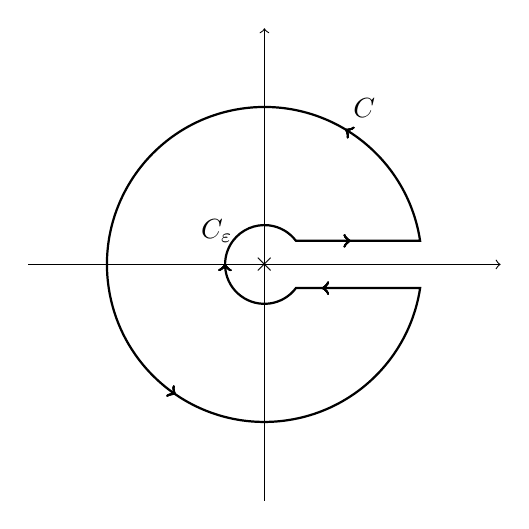
\begin{tikzpicture}
      \draw [->] (-3, 0) -- (3, 0);
      \draw [->] (0, -3) -- (0, 3);

      \draw [black, thick, ->-=0.1, ->-=0.45, ->-=0.75, ->-=0.84, ->-=0.95] (1.977, 0.3) arc(8.63:351.37:2) node [pos=0.15, anchor = south west] {$C$} -- (0.4, -0.3) arc(323.13:36.87:0.5) node [pos=0.7, left] {$C_\varepsilon$} -- cycle;

      \node [circle] at (0, 0) {$\times$};
    \end{tikzpicture}
  \end{center}
Now suppose the surface does intersect the $z$-axis, then the closed loop integral would be
$$\oint_{C'}\mathbf{v}\cdot d\mathbf{r}=\int_0^{2\pi}\mathbf{v}\cdot\frac{d\mathbf{r}}{d\theta} d\theta=\frac{\kappa}{2\pi}\oint\frac{xdy-ydx}{x^2+y^2}=\frac{\kappa}{2\pi}\int_0^{2\pi} d\theta=\kappa$$
Physically, one can imagine the $z$-axis to be a source of strength $\kappa$, i.e. similar to Ampere's Law in magnetostatics.
\end{enumerate}
\end{enumerate}
\end{ans}
\newpage
\begin{qns}[Partial Differential Equation]\leavevmode
\begin{enumerate}[label=(\alph*)]
    \item Consider diffusion inside a circular tube with very small cross-section and circumference $2\pi$. Let $x$ denote the arc-length parameter $-\pi\leq x\leq\pi$, so that the density of the diffusing substance $u$ satisfies (for $t>0$)
$$\frac{\partial u}{\partial t}=\lambda\frac{\partial^2u}{\partial x^2}$$
with specified initial conditions $u(x,0)=f(x)$ for some function $f(x)$. What are the appropriate boundary conditions to impose on $u$ at $x=\pm\pi$ for $t>0?$\hfill \textbf{[3]}
\item Use separation of variables to express $u(x,t)$ in terms of an appropriate infinite series.\hfill \textbf{[7]}
\item Compute explicitly the coefficients of the above series in the case that $f(x)=(\pi-|x|)^2$ and identify the density distribution of the substance $u$ as $t\rightarrow\infty$.\hfill \textbf{[10]}
\end{enumerate}
\end{qns}
\begin{ans}\leavevmode
\begin{enumerate}[label=(\alph*)]
    \item We integrate the PDE over an infinitesimal region of $x$,
$$\lim_{\epsilon\rightarrow0}\lambda\int_{x-\epsilon}^{x+\epsilon}\frac{\partial^2u}{\partial x'^2}dx'=\lim_{\epsilon\rightarrow0}\int_{x-\epsilon}^{x+\epsilon}\frac{\partial u}{\partial t}dx'=0$$
We thus have $\frac{\partial}{\partial x}u$ to be continuous everywhere and hence $u$ have to be continuous everywhere. This includes the endpoints $x=\pm\pi$. This is known as periodic boundary conditions.
\item Using separation of variables, $u(x,t)=X(x)T(t)$, then we have
$$\frac{T'}{T}=\lambda\frac{X''}{X}=-n^2\lambda$$
for $\lambda>0$ and $n^2>0$. Such a choice is necessary to ensure $X(x)$ satisfy the periodic boundary conditions. Hence, $X(x)=c_1\cos(n x)+c_2\sin(n x)$. Hence, $\frac{dT}{T}=-n^2\lambda dt\implies T(t)=ce^{-n^2\lambda t}$. The general solution will thus be
$$u(x,t)=C+\sum_{n=1}^\infty e^{-n^2\lambda t}[A_n\cos(nx)+B_n\sin(nx)]$$
\item We have initial condition $u(x,0)=f(x)=(\pi-|x|)^2$ (which is even). To find the Fourier coefficients,
$$B_n=\frac{1}{\pi}\int_{-\pi}^\pi f(x)\sin(nx)dx=0\text{ since even}$$
$$C=\frac{1}{2\pi}\int_{-\pi}^\pi f(x)dx=\frac{1}{2\pi}2\int_0^\pi(\pi-x)^2dx=\frac{\pi^2}{3}$$
$$A_n=\frac{1}{\pi}\int_{-\pi}^\pi f(x)\cos(nx)dx=\frac{1}{\pi}2\int_0^\pi(\pi-x)^2\cos(nx)dx=\frac{4}{n\pi}\bigg(\frac{\pi}{n}-\frac{1}{n^2}[\sin(nx)]^\pi_0\bigg)=\frac{4}{n^2}$$
Hence, in large times $t>>1$:
$$\lim_{t\rightarrow\infty}u(x,t)=\frac{\pi^2}{3}+\lim_{t\rightarrow\infty}\sum_{n=1}^\infty\frac{4}{n^2}\cos(nx)e^{-\lambda n^2t}=\frac{\pi^2}{3}$$
\end{enumerate}
\end{ans}
\newpage
\begin{qns}[Green's Functions]\leavevmode
\begin{enumerate}[label=(\alph*)]
    \item Consider a linear differential operator $\mathcal{L}$ defined by
$$\mathcal{L}y=-\frac{1}{x^2}\frac{d}{dx}\bigg(x^2\frac{dy}{dx}\bigg)+y$$
for $0<x<+\infty$. By writing $y=z/x$ or otherwise, find those solutions of $\mathcal{L}y=0$ which are either (i) bounded as $x\rightarrow0$, or (ii) bounded as $x\rightarrow+\infty$.\hfill \textbf{[5]}
\item Find the Green's function $G(x,\xi)$ satisfying
$$\mathcal{L}G(x,\xi)=\delta(x-\xi)$$
such that $G$ is bounded as $x\rightarrow0$ and $G$ is bounded as $x\rightarrow+\infty$.\hfill \textbf{[8]}
\item  Use $G(x,\xi)$ to solve
$$\mathcal{L}y=
\left\{
        \begin{array}{ll}
      1 & 0\leq x\leq R \\
      0 & x>R
        \end{array}
    \right.$$
with $y$ bounded as $x\rightarrow0$ and $x\rightarrow+\infty$.\\[5pt]
[It is convenient to consider the solution for $x>R$ and $x<R$ separately.]\hfill \textbf{[7]}
\end{enumerate}
\end{qns}
\begin{ans}\leavevmode
\begin{enumerate}[label=(\alph*)]
\item Upon using this substitution, we have
$$\mathcal{L}(z/x)=-\frac{1}{x}\frac{d^2z}{dx^2}+\frac{z}{x}$$
The corresponding solution will be
$$y=\frac{1}{x}(c_1e^x+c_2e^{-x})$$
For (i), $c_1=-c_2$; for (ii), $c_1=0$.
\item The corresponding Green's function satisfy $\mathcal{L}G(x,\xi)=\delta(x-\xi)$ and the b.c.s. ($G$ is bounded as $x\rightarrow 0$ and $x\rightarrow+\infty$). The equation is homogeneous when $x\neq\xi$. Using the homogeneous solution in part (a),
$$G(x,\xi)=
\left\{
        \begin{array}{ll}
      A(\xi)\frac{\sinh(x)}{x} & 0\leq x<\xi<\infty\\
      B(\xi)\frac{e^{-x}}{x} & 0\leq\xi<x<\infty
        \end{array}
    \right.$$
We can integrate $\mathcal{L}G(x,\xi)$ over an infinitesimal region about $x=\xi$, to obtain the jump condition $[\frac{\partial G}{\partial x}]_-^+=-1$ at $x=\xi$. Also, $G$ has to be continuous everywhere, including $x=\xi$ (otherwise $G''\propto\delta'(x-\xi)$ which leads to a contradiction). At $x=\xi$, we have the jump and continuity conditions to be respectively
$$-A(\xi)\frac{\cosh(\xi)}{\xi}+\frac{A(\xi)}{\xi^2}\sinh(\xi)-B(\xi)\frac{e^{-\xi}}{\xi}-\frac{B(\xi)}{\xi^2}e^{-\xi}=-1$$
$$\frac{\sinh(\xi)}{\xi}A(\xi)=B(\xi)\frac{e^{-\xi}}{\xi}$$
With both conditions, we have $A=\xi e^{-\xi}$ and $B=\xi\sinh\xi$. Hence, $G(x,\xi)=\xi e^{-\xi}\sinh(x)/x$ for $0\leq x\leq\xi$ and $G(x,\xi)=\xi\sinh\xi e^{-x}/x$ for $0\leq\xi\leq x$. \item The solution is
$$y=\int_0^\infty G(x,\xi)f(\xi)d\xi=\frac{e^{-x}}{x}\int_0^x\xi\sinh\xi f(\xi) d\xi+\frac{\sinh(x)}{x}\int_x^\infty\xi e^{-\xi}f(\xi)d\xi$$
We first consider the case $x<R$,
$$y=\frac{e^{-x}}{x}\int_0^x\xi\sinh\xi d\xi+\frac{\sinh(x)}{x}\int_x^R\xi e^{-\xi}d\xi=\frac{\sinh(x)}{x}[(2+x)e^{-x}-(1+R)e^R]$$
and then $x>R$,
$$y=\frac{e^{-x}}{x}\int_0^R\xi\sinh\xi d\xi=\frac{e^{-x}}{x}[1-(1+R)e^{-R}]$$
\end{enumerate}
\end{ans}
\newpage
\begin{qns}[Fourier Transform]\leavevmode
\begin{enumerate}[label=(\alph*)]
    \item Calculate the Fourier transform of the function
$$g(x)=e^{-\lambda|x|}$$
where $\lambda$ is a positive constant, and hence or otherwise calculate the Fourier transform of the function
$$h(x)=\frac{1}{x^2+\mu^2}$$
where $\mu$ is a positive constant.\hfill \textbf{[8]}
\item Consider Laplace's Equation for $\psi(x,y)$ in the half-plane with prescribed boundary conditions at $y=0$, i.e.
$$\frac{\partial^2\psi}{\partial x^2}+\frac{\partial^2\psi}{\partial y^2}=0;\quad -\infty<x<\infty,~y\geq0$$
where $\psi(x,0)=f(x)$ is a known function with a well-defined Fourier transform, and where $\psi\rightarrow0$ as $y\rightarrow\infty$, and $f(x)\rightarrow0$ as $|x|\rightarrow\infty$.\\[5pt]
By taking the Fourier transform with respect to $x$, and applying the convolution theorem (which may be quoted without proof), show that\hfill \textbf{[8]}
$$\psi(x,y)=\frac{y}{\pi}\int_{-\infty}^\infty\frac{f(u)}{(x-u)^2+y^2}du$$
\item Find (in closed form) the solution when \hfill \textbf{[4]}
$$f(x)=
\left\{
        \begin{array}{ll}
      c=\text{constant} & |x|<a \\
      0 & \text{otherwise}
        \end{array}
    \right.$$
\end{enumerate}
\end{qns}
\begin{ans}\leavevmode
\begin{enumerate}[label=(\alph*)]
\item Evaluate the Fourier transform of $g$, $\tilde{g}$:
$$\frac{1}{\sqrt{2\pi}}\int_{-\infty}^\infty e^{-\lambda|x|}e^{-ikx}dx=\frac{1}{\sqrt{2\pi}}\bigg(\int_{-\infty}^0e^{x(\lambda-ik)}dx+\int_0^\infty e^{-x(\lambda+ik)}dx\bigg)=\frac{1}{\sqrt{2\pi}}\bigg(\frac{1}{\lambda-ik}+\frac{1}{\lambda+ik}\bigg)$$
which is $\frac{1}{\sqrt{2\pi}}\frac{2\lambda}{\lambda^2+k^2}$, so by Fourier inversion theorem,
$$\mathcal{F}\bigg[\frac{1}{x^2+\mu^2}\bigg]=\mathcal{F}[\tilde{g}(x)]\frac{\sqrt{2\pi}}{2\mu}=e^{-\mu|k|}\frac{1}{\mu}\sqrt{\frac{\pi}{2}}$$
\item  Take the Fourier transform of the Laplace's equation w.r.t $x$,
$$0=\int_{-\infty}^\infty\bigg(\frac{\partial^2\psi}{\partial x^2}+\frac{\partial^2\psi}{\partial y^2}\bigg)e^{-ikx}dx=\bigg[\frac{\partial\psi}{\partial x}e^{-ikx}\bigg]^\infty_{-\infty}+ik\int_{-\infty}^\infty\frac{\partial\psi}{\partial x}e^{-ikx}dx+\frac{\partial^2\tilde{\psi}}{\partial y^2}=[ik\psi e^{-ikx}]^\infty_{-\infty}-k^2\tilde{\psi}+\frac{\partial^2\tilde{\psi}}{\partial y^2}$$
where we note that $\psi\rightarrow 0$ as $y\rightarrow\infty$. We thus have $\tilde{\psi}(k,y)=A(k)e^{-ky}+B(k)e^{ky}$. Naturally, $\tilde{\psi}$ vanish as $y\rightarrow\infty$ so $\tilde{\psi}(k,y)=D(k)e^{-y|k|}$. Using the convolution theorem,  $$\tilde{v}=\tilde{a}\tilde{b}\implies v=\frac{1}{\sqrt{2\pi}}a*b$$ and the fact that $D(k)$ obtained from the Fourier Transform of $\psi(x,0)$, 
$$\psi(x,y)=\frac{1}{\sqrt{2\pi}}\int_{-\infty}^\infty\psi(x,0)\frac{1}{\sqrt{2\pi}}\frac{2y}{y^2+(x-u)^2}du=\frac{y}{\pi}\int_{-\infty}^\infty\frac{f(x)}{y^2+(x-u)^2}du$$
where $f(x)=\psi(x,0)$.
\item Using substitution, $x-u=y\tan\theta$, we have $\psi(x,y)$ to be
$$\frac{y}{\pi}\int_{\tan^{-1}((-a-x)/y)}^{\tan^{-1}((a-x)/y)}\frac{c}{y^2(1+\tan^2\theta)}y\sec^2\theta d\theta=\frac{c}{\pi}\bigg[\tan^{-1}\bigg(\frac{a-x}{y}\bigg)-\tan^{-1}\bigg(\frac{-a-x}{y}\bigg)\bigg]$$
such that $\tan^{-1}$ is consistent with $y\geq0$.
\end{enumerate}
\end{ans}
\newpage
\begin{qns}[Linear Algebra]\leavevmode
\begin{enumerate}[label=(\alph*)]
    \item What is (i) an eigenvalue, and (ii) an eigenvector, of a complex $n\times n$ matrix $A$? Show that $A$ has at least one eigenvector.\hfill \textbf{[3]}
    \item Give an example of a non-diagonalizable $n\times n$ matrix for some $n$.\hfill \textbf{[2]}
    \item What is a Hermitian matrix? Explain briefly why a Hermitian matrix can always be diagonalized.\hfill \textbf{[3]}
    \item In the remainder of this question, $A$ is a Hermitian matrix. Now assume that $\mathbf{e_i}$ for $i=1,...,n$ is a complete set of eigenvectors for $A$, with corresponding eigenvalues $\lambda_i$. Prove that the eigenvalues $\lambda_i$ are real.\hfill \textbf{[1]}
    \item Assume from now on that all the eigenvalues are negative, i.e. $\lambda_i<0$. Obtain complete sets of eigenvectors and eigenvalues for $A^{-1}$ and $A^n$ $\forall n\in\mathbb{Z}^+$.\hfill \textbf{[4]}
    \item Prove that\hfill \textbf{[7]}
$$A^{-1}=\int_0^\infty e^{tA}dt$$
\end{enumerate}
\begin{mdframed}
\textcolor{darkblue}{You may use without proof that any complex polynomial has a complex zero. If $B$ is a matrix, then $e^B=\sum_{n=0}^\infty\frac{B^n}{n!}$. If $B(t)$ is a matrix depending on $t$ with entries $B_{ij}(t)$, then $\int_0^\infty B(t)dt$ means the matrix with entries $\int_0^\infty B_{ij}(t)dt$, when these integrals exist.}
\end{mdframed}
\end{qns}
\begin{ans}\leavevmode
\begin{enumerate}[label=(\alph*)]
\item If $\lambda$ is an eigenvalue of the matrix $A$, then $\exists v\neq 0$ such that $Av=\lambda v$. The characteristic polynomial of $A$ is $\chi_A(\lambda)=\det(A-\lambda I)$ which is complex since $A$ is complex. By the fundamental theorem of algebra, $\chi_A(\lambda)$ has at least one root. There is thus at least one eigenvalue and therefore at least one eigenvector, which is the corresponding eigenvector to this eigenvalue.
\item Consider the matrix
$$A=\begin{pmatrix}1&1\\0&1\\\end{pmatrix}$$
Then its characteristic equation is given by
$$\det\begin{pmatrix}1-\lambda&1\\0&1-\lambda\\\end{pmatrix}=0\implies(1-\lambda)^2=0\implies\lambda=1$$
so if it were to be diagonalizable, then $\exists$ an invertible matrix $R$ such that $R^{-1}AR=\diag(1,1)\implies A=I$ which contradicts. Hence, $A$ is not diagonalizable.
\item The matrix $A$ is Hermitian if $A^\dag=A$. Since $A$ is Hermitian, then the eigenvectors corresponding to distinct eigenvalues must be pairwise orthogonal. If $A$ has $n$ distinct eigenvalues, we will have $n$ linearly independent eigenvectors and has $n$ linearly independent eigenvectors, which can be normalized to obtain an orthonormal basis. If not, there will be say $r<n$ distinct eigenvalues, then we can extend the basis of $r$ eigenvectors to $\mathbb{C}^n$ and use Gram-Schmidt procedure to obtain an orthonormal basis of $n$ vectors. Regardless, we can always construct a unitary matrix $R$ whose columns are the orthonormal vectors such that $R^TAR$ will be a diagonal matrix.
\item Let the corresponding eigenvalue for the eigenvector $\mathbf{e_i}$ be $\lambda_i$ such that $A\mathbf{e_i}=\lambda_i\mathbf{e_i}$. Multiplying $\mathbf{e_i}^\dag$ from the left on both sides, we have
$$\lambda_i\mathbf{e_i}^\dag\mathbf{e_i}=\mathbf{e_i}^\dag A\mathbf{e_i}=(A\mathbf{e_i})^\dag\mathbf{e_i}=\lambda_i^*\mathbf{e_i}^\dag\mathbf{e_i}$$
This means $(\lambda_i^*-\lambda_i)\mathbf{e_i}^\dag\mathbf{e_i}=0$. Since $\mathbf{e_i}\neq\boldsymbol{0}$, then $\mathbf{e_i}^\dag\mathbf{e_i}\neq0$, we must have $\lambda_i=\lambda_i^*\in\mathbb{R}$ $\forall i$.
\item We have 
$$A^n\mathbf{e_i}=A^{n-1}\lambda_i\mathbf{e_i}=\dots=(\lambda_i)^n\mathbf{e_i}$$
as long as the eigenvalue is not zero. This also works for $n=-1$, i.e.
$$A^{-1}\mathbf{e_i}=\frac{1}{\lambda_i}\mathbf{e_i}$$
And so the eigenvectors of $A$ are also the eigenvectors of $A^n$ with eigenvalues $\lambda_i^n$.
\item Consider any vector $\mathbf{v}$. Since the eigenvectors of $A$ form a complete set, then they form an eigenbasis. we may decompose $\mathbf{v}$ in terms of this eigenbasis, i.e. $\mathbf{v}=\sum_{p=1}^n\alpha_p\mathbf{e_p}$. We thus have $\int_0^\infty e^{tA}\mathbf{v}dt$ to be
\begin{align}
\int_0^\infty\bigg(\sum_{q=0}^\infty\frac{t^qA^q}{q!}\bigg)\bigg(\sum_{p=1}^n\alpha_p\mathbf{e_p}\bigg)dt&=\sum_{p=1}^n\alpha_p\int_0^\infty\sum_{q=0}^\infty\frac{t^q\lambda_p^q}{q!}\mathbf{e_p}dt\nonumber\\&=\sum_{p=1}^n\alpha_p\mathbf{e_p}\int_0^\infty e^{t\lambda_p}dt\nonumber\\&=-\sum_{p=1}^n\alpha_p\mathbf{e_p}\lambda_p^{-1}\nonumber
\end{align}
where we handwavingly swap the infinite sum with the integral. 
Since all the eigenvalues are negative, the upper limit vanishes. Moreover, we have from part e, $$A^{-1}\mathbf{v}=A^{-1}\sum_{p=1}^n\alpha_p\mathbf{e_p}=\sum_{p=1}^n\frac{\alpha_p}{\lambda_p}\mathbf{e_p}$$
so $A^{-1}=-\int_0^\infty e^{tA}dt$ as requested.
\end{enumerate}
\end{ans}
\begin{qns}[Linear Algebra]\leavevmode
\begin{enumerate}[label=(\alph*)]
    \item Give a real linear transformation $\mathbf{x}=L\mathbf{y}$ which converts the quadratic form $Q_1(\mathbf{x})=x_1^2+4x_1x_2+5x_2^2+6x_3^2$ into $\tilde{Q}_1(\mathbf{y})=y_1^2+y_2^2+y_3^2$. What is the corresponding result for the quadratic form $Q_2(\mathbf{x})=x_1^2+4x_1x_2+5x_2^2-6x_3^2$?\hfill \textbf{[5]}
    \item Define the trace $\Tr(A)$ of a square matrix $A$, and prove that $\Tr(AB)=\Tr(BA)$. For which complex numbers $c$ do there exist $n\times n$ matrices $A$, $B$ such that
$$AB-BA=cI$$
where $I$ is the identity matrix? For each complex number $c$ either give an example or prove the non-existence of such matrices.\hfill \textbf{[6]}
\item Let $A(\epsilon)$ be a symmetric $n\times n$ matrix for each real $\epsilon$. The smallest eigenvalue of $A(\epsilon)$ is $\lambda(\epsilon)$, with corresponding real eigenvector $\mathbf{x}=\mathbf{x}(\epsilon)$ normalized so that $\mathbf{x}^T\mathbf{x}=1$ $\forall\epsilon$, where $^T$ denotes transpose. Assuming that $A(\epsilon)$, $\lambda(\epsilon)$, $\mathbf{x}(\epsilon)$ vary smoothly with $\epsilon$, show that\hfill \textbf{[9]}
$$\frac{d\lambda}{d\epsilon}\bigg|_{\epsilon=0}=\mathbf{x^T}\frac{dA}{d\epsilon}\mathbf{x}\bigg|_{\epsilon=0}$$
where $^T$ denotes transpose.
\end{enumerate}
\end{qns}
\newpage
\begin{ans}\leavevmode
\begin{enumerate}[label=(\alph*)]
\item We write $Q_1$ as a quadratic form
$$Q_1(\mathbf{x})=\begin{pmatrix}x_1\\x_2\\x_3\\\end{pmatrix}^T\begin{pmatrix}1&2&0\\2&5&0\\0&0&6\\\end{pmatrix}\begin{pmatrix}x_1\\x_2\\x_3\\\end{pmatrix}=x^TMx$$
$$\det(M-\lambda I)=\det\begin{pmatrix}1-\lambda&2&0\\2&5-\lambda&0\\0&0&6-\lambda\\\end{pmatrix}=0\implies(6-\lambda)(\lambda-3-2\sqrt{2})(\lambda-3+2\sqrt{2})=0$$
By inspection, the eigenvector for $\lambda=6$ is $(0,0,1)^T$. For $\lambda=3\pm 2\sqrt{2}$, we have
$$\begin{pmatrix}-2\mp2\sqrt{2}&2&0\\2&2\mp\sqrt{2}&0\\0&0&3\pm2\sqrt{2}\\\end{pmatrix}\begin{pmatrix}x_1\\x_2\\x_3\\\end{pmatrix}=0$$
which gives $\frac{1}{\sqrt{3}}(1,1\pm\sqrt{2},0)^T$. We can construct an orthogonal matrix $R$ by having the normalized eigenvectors as its rows such that $M'=RMR^T$ is a diagonal matrix with diagonal entries as the corresponding eigenvalues. Further, we can write $M'=PIP$ so that we associate $\mathbf{y}=PR\mathbf{x}$, thus
$$Q_1=\mathbf{x}^TR^TPIPR\mathbf{x}=\mathbf{y}^TI\mathbf{y}=y_1^2+y_2^2+y_3^2$$
The requested linear transformation is $L=PR$:
$$L=\begin{pmatrix}\sqrt{6}&0&0\\0&\sqrt{3+2\sqrt{2}}&0\\0&0&\sqrt{3-2\sqrt{2}}\\\end{pmatrix}\begin{pmatrix}0&1/\sqrt{3}&1/\sqrt{3}\\0&\frac{1}{\sqrt{3}}(1+\sqrt{2})&\frac{1}{\sqrt{3}}(1-\sqrt{2})\\1&0&0\\\end{pmatrix}$$
For $Q_2$, we have $-y_1^2+y_2^2+y_3^2$ due to the eigenvalue of the $x_3$ direction now being $-6$ instead of $+6$.
\item The trace is $\sum_{i=1}^na_{ii}$ and so 
$$\Tr(AB)=\sum_{i=1}^n(AB)_{ii}=\sum_{i=1}^n\sum_{j=1}^na_{ij}b_{ji}=\sum_{j=1}^n(BA)_{jj}=\Tr(BA)$$
Taking the trace of the given expression, we have $\Tr(AB-BA)=\Tr(cI)=cn$. Hence, $c=0$. One example would be $A=I$, $B=\sigma_z$ (Pauli spin matrix).
\item Consider the Rayleigh quotient $\Lambda=\frac{\mathbf{x}^TA\mathbf{x}}{\mathbf{x}^T\mathbf{x}}$. If $\mathbf{x}$ is an eigenvector, then this quotient is simply the eigenvalue $\lambda$, i.e. $Ax=\lambda x$. Differentiating both sides with respect to $\epsilon$, we have
\begin{align}
\frac{d\lambda}{d\epsilon}&=\frac{1}{\mathbf{x}^T\mathbf{x}}\bigg(\frac{d\mathbf{x}^T}{d\epsilon}A\mathbf{x}+\mathbf{x}^T\frac{dA}{d\epsilon}\mathbf{x}+\mathbf{x}^TA\frac{d\mathbf{x}}{d\epsilon}\bigg)-\frac{\mathbf{x}^TA\mathbf{x}}{(\mathbf{x}^T\mathbf{x})^2}\bigg(\frac{d\mathbf{x}^T}{d\epsilon}\mathbf{x}+\mathbf{x}^T\frac{d\mathbf{x}}{d\epsilon}\bigg)\nonumber\\&=\frac{1}{\mathbf{x}^T\mathbf{x}}\bigg(\frac{d\mathbf{x}^T}{d\epsilon}\lambda\mathbf{x}+\mathbf{x}^T\frac{dA}{d\epsilon}\mathbf{x}+\lambda\mathbf{x}^T\frac{d\mathbf{x}}{d\epsilon}\bigg)-\frac{\lambda}{\mathbf{x}^T\mathbf{x}}\bigg(\frac{d\mathbf{x}^T}{d\epsilon}\mathbf{x}+\mathbf{x}^T\frac{d\mathbf{x}}{d\epsilon}\bigg)\nonumber\\&=\mathbf{x}^T\frac{dA}{d\epsilon}\mathbf{x}\nonumber
\end{align}
where $\mathbf{x}^T\mathbf{x}=1$, $A\mathbf{x}=\lambda\mathbf{x}$, $\mathbf{x}^TA=(A\mathbf{x})^T=\lambda\mathbf{x}^T$ since $A$ is symmetric. Hence, we obtained our desired result (true $\forall\epsilon$, especially $\epsilon=0$).
\end{enumerate}
\end{ans}
\newpage
\begin{qns}[Cauchy-Riemann]\leavevmode
\begin{enumerate}[label=(\alph*)]
    \item Obtain the Cauchy-Riemann equations for the analytic function \hfill \textbf{[2]}$$f(z)=u(x,y)+iv(x,y)$$
    \item Show that:
    \begin{enumerate}[label=(\roman*)]
        \item $u$ and $v$ satisfy the Laplace's equation, $\nabla^2u=\nabla^2v=0$; \hfill \textbf{[2]}
        \item the level sets constant $u$ and constant $v$ are orthogonal, i.e. $\boldsymbol{\nabla}u\cdot\boldsymbol{\nabla}v=0$; \hfill \textbf{[2]}
        \item every stationary point of $u$ is a stationary point of $v$ and conversely; \hfill \textbf{[2]}
        \item stationary points for which
        $\begin{vmatrix}\partial_{xx}u&\partial_{xy}u\\\partial_{yx}u&\partial_{yy}u\\\end{vmatrix}\neq0$ must be saddle points;\hfill \textbf{[4]}
    \item If $f(z)=u(x,y)+iv(x,y)$ and $g(z)=s(x,y)+it(x,y)$ are analytic functions, then so is $g(f(z))$, and hence deduce that $s(u(x,y),v(x,y))$ satisfies Laplace's equation.\hfill \textbf{[8]}
    \end{enumerate}
\end{enumerate}
\end{qns}
\begin{ans}\leavevmode
\begin{enumerate}[label=(\alph*)]
\item The Cauchy-Riemann equations are obtained by requiring the existence of $$f'(z)=\lim_{\delta z\rightarrow0}\frac{f(z+\delta z)-f(z)}{\delta z}$$ This value should be independent of the direction of approach for $\delta z\rightarrow 0$. We can take any two linearly independent directions, say $\delta z=\delta x$ and $\delta z=i\delta y$. 
$$\lim_{\delta x\rightarrow0}\frac{u(x+\delta x,y)+iv(x+\delta x,y)}{\delta x}=\lim_{\delta y\rightarrow0}\frac{u(x,y+\delta y)+iv(x,y+\delta y)}{i\delta y}\implies\frac{\partial u}{\partial x}+i\frac{\partial v}{\partial x}=-i\frac{\partial u}{\partial y}+\frac{\partial v}{\partial y}$$
This gives us the Cauchy-Riemann equations, namely $\frac{\partial u}{\partial x}=\frac{\partial v}{\partial y}$ and $\frac{\partial u}{\partial y}=-\frac{\partial v}{\partial x}$.
\item
\begin{enumerate}[label=(\roman*)]
\item We have the Laplacian of $u$ to be
$$\nabla^2u=\frac{\partial^2u}{\partial x^2}+\frac{\partial^2u}{\partial y^2}=\frac{\partial}{\partial x}\frac{\partial v}{\partial y}+\frac{\partial}{\partial y}\bigg(-\frac{\partial v}{\partial x}\bigg)=0$$
Similar for $v$, hence $u$ and $v$ satisfy the Laplace's equation.
\item Evaluating $\boldsymbol{\nabla}u\cdot\boldsymbol{\nabla}v$ with the Cauchy-Riemann equations
$$\boldsymbol{\nabla}u\cdot\boldsymbol{\nabla}v=\frac{\partial u}{\partial x}\frac{\partial v}{\partial x}+\frac{\partial u}{\partial y}\frac{\partial v}{\partial y}=\frac{\partial v}{\partial y}\frac{\partial v}{\partial x}-\frac{\partial v}{\partial x}\frac{\partial v}{\partial y}=0$$
\item If we have a stationary point of $u$, then $\frac{\partial u}{\partial x}=\frac{\partial u}{\partial y}=0$. By Cauchy-Riemann, then $\frac{\partial v}{\partial x}=\frac{\partial v}{\partial y}=0$, and hence a stationary point of $v$.
\item Evaluating the Hessian, we have
$$\frac{\partial}{\partial x}\frac{\partial u}{\partial x}\times\frac{\partial}{\partial y}\frac{\partial u}{\partial y}-\bigg(\frac{\partial^2u}{\partial x\partial y}\bigg)^2=-\bigg(\frac{\partial^2v}{\partial x\partial y}\bigg)^2-\bigg(\frac{\partial^2u}{\partial x\partial y}\bigg)^2<0$$
For a function of 2 variables $u(x,y)$, if the determinant of the Hessian is negative at this point, this point is a saddle point.
\item We have $f(x+iy)=u(x,y)+iv(x,y)$ to be analytic, then $f$ satisfies the Cauchy-Riemann equations, i.e. $(\frac{\partial u}{\partial x})_y=(\frac{\partial v}{\partial y})_x$ and $(\frac{\partial u}{\partial y})_x=-(\frac{\partial v}{\partial x})_y$. Similarly, $g(u+iv)=s(u,v)+it(u,v)$ is analytic, this gives $(\frac{\partial s}{\partial v})_u=(\frac{\partial t}{\partial v})_u$ and $(\frac{\partial s}{\partial v})_u=-(\frac{\partial t}{\partial u})_v$. Consider the composite function
$$g(f(z))=s(u(x,y),v(x,y))+it(u(x,y),v(x,y))$$
then we have by chain rule,
$$\bigg(\frac{\partial s}{\partial x}\bigg)_y=\bigg(\frac{\partial u}{\partial x}\bigg)_y\bigg(\frac{\partial s}{\partial u}\bigg)_v+\bigg(\frac{\partial v}{\partial x}\bigg)_y\bigg(\frac{\partial s}{\partial v}\bigg)_u=\bigg(\frac{\partial v}{\partial y}\bigg)_x\bigg(\frac{\partial t}{\partial v}\bigg)_u+\bigg(\frac{\partial t}{\partial u}\bigg)_v\bigg(\frac{\partial u}{\partial y}\bigg)_x=\bigg(\frac{\partial t}{\partial y}\bigg)_x$$
$$\bigg(\frac{\partial s}{\partial y}\bigg)_x=\bigg(\frac{\partial u}{\partial y}\bigg)_x\bigg(\frac{\partial s}{\partial u}\bigg)_v+\bigg(\frac{\partial v}{\partial y}\bigg)_x\bigg(\frac{\partial s}{\partial v}\bigg)_u=-\bigg(\frac{\partial v}{\partial x}\bigg)_y\bigg(\frac{\partial t}{\partial v}\bigg)_u-\bigg(\frac{\partial t}{\partial u}\bigg)_v\bigg(\frac{\partial u}{\partial x}\bigg)_y=\bigg(\frac{\partial t}{\partial x}\bigg)_y$$
Hence composite functions obey the Cauchy-Riemann equations. By part (a), we can thus conclude $s(u,v)$ satisfy the Laplace's equation.
\end{enumerate}
\end{enumerate}
\end{ans}
\newpage
\begin{qns}[Series Solution to ODE]\leavevmode
\begin{enumerate}[label=(\alph*)]
    \item Show that the origin is an ordinary point, and that $x=1$ and $x=-1$ are regular singular points of the equation
\begin{equation}
(1-x^2)\frac{d^2y}{dx^2}-x\frac{dy}{dx}+p^2y=0\tag{*}
\end{equation}
where $p$ is a real constant.\hfill \textbf{[4]}
\item You may assume that there are two linearly independent series solutions of the form $$y_q=x^q\sum_{n=0}^\infty a_nx^n, \quad q=0,1$$
Find the recurrence relations for $a_n$ for the two cases, and show that the series converges for $|x|<1$.\hfill \textbf{[6]}
\item Show that polynomial solutions $T_m(x)$ exist for $p=m$, where $m$ is a non-negative integer. With the condition $T_m(1)=1$, calculate all the coefficients for the cases $m=0,1,2,3$.\hfill \textbf{[6]}
\item For $-1\leq x\leq 1$, make the substitution $x=\cos\theta$ with $0\leq\theta\leq\pi$, in the above differential equation (*). Hence, or otherwise, show that $T_m(x)=\cos(m\cos^{-1}(x))$ for any non-negative integer $m$. \hfill \textbf{[4]}
\end{enumerate}
\end{qns}
\begin{ans}\leavevmode
\begin{enumerate}[label=(\alph*)]
\item Write the ordinary differential equation as  
$\frac{d^2y}{dx^2}-\frac{x}{1-x^2}\frac{dy}{dx}+\frac{p^2}{1-x^2}y=0$. We see that $-\frac{x}{1-x^2}$ and $\frac{p^2}{1-x^2}$ are analytic at $x=0$, but not analytic at $x=\pm 1$. But, $-\frac{(x\mp 1)x}{1-x^2}=-\frac{x}{1\pm x}$ and $-\frac{p^2(x\mp1)^2}{1-x^2}=\frac{x(1\mp x)}{1\pm x}$ are analytic at $x=\pm 1$. So $x=0$ is an ordinary point while $x=\pm 1$ are regular singular points.
\item Use a Frobenius series solution  $y_q=\sum_{n=0}^\infty a_nx^{n+q}$, and so
$$\sum_{n=0}^\infty a_n(n+q)(n+q-1)x^{n+q-2}-\sum_{n=0}^\infty a_n(n+q)(n+q-1)x^{n+q}-\sum_{n=0}^\infty a_n(n+q)x^{n+q}+p^2\sum_{n=0}^\infty a_nx^{n+q}=0$$
Comparing coefficients for $x^{q-2}$, we have the indicial equation $a_0q(q-1)=0$. Since we are given $q=0,1$, we must have $a_0\neq 0$. Comparing coefficients for $x^{q-1}$, we have $a_1q(1+q)=0$. For $q=0$, free to choose $a_1=0$. For $q=1$, we have $q(1+q)\neq 0$ and thus $a_1=0$ must be true. Comparing coefficients for $x^{n+q}$ where $n\geq0$, then we obtain the recurrence relation
$$a_{n+2}(n+q+2)(n+q+1)-a_n(n+q)(n+q-1+1-p^2)=0\implies\frac{a_{n+2}}{a_n}=\frac{(n+q)^2-p^2}{(n+q+2)(n+q+1)}$$
for $q=0,1$. For the series to converge $\forall|x|<1$, we require $\lim_{n\rightarrow\infty}|\frac{a_{n+2}}{a_n}||x^2|<1$. We have 
$$|x|^2<\lim_{n\rightarrow\infty}\bigg|\frac{(n+q+2)(n+q+1)}{(n+q)^2-p^2}\bigg|<1$$
\item We will obtain polynomial solutions if the recurrence relation terminates for some $i$, where $i\in\mathbb{Z}^+\cup\{0\}$. This requires $(i+q)^2=p^2\implies i+q=p$.
\begin{itemize}
    \item $m=p=0$: $i+q=0\implies q=\implies T_0=a_0x^0$. Normalization: $T_0(1)=a_0=1$ $\forall x$;
    \item $m=p=1$: $i+q=1$. $q=0$ give no valid solution while $q=1$ give $i=0$ and so $T_1(x)=a_0x$. Normalization: $T_1(1)=a_0=1$ $\forall x$, so $T_1(x)=x$;
    \item $m=p=2$: $i+q=2$. $q=0$ gives $\frac{a_2}{a_0}=\frac{-2^2}{2}=-2$. Series terminates at $n=2$. Normalization: $T_2(1)=1\implies a_0=-1$ $\forall x$, so $T_2(x)=2x^2-1$;
    \item $m=p=3$: $i+q=3$. If $q=0$, $a_1=0$, $\frac{a_2}{a_3}=\frac{3^2-3^2}{(3+0+2)(3+0+1)}=0$, so no valid solution. If $q=1$ and $i=2$, $\frac{a_2}{a_0}=\frac{1-3^2}{(1+2)(1+1)}=\frac{-4}{3}$. Normalization: $T_3(1)=1\implies a_0=-3$ $\forall x$, so $T_3(x)=-3x+4x^3$.
\end{itemize}
\item We have $x=\cos\theta$, and so $\frac{d}{dx}=-\frac{1}{\sin\theta}\frac{d}{d\theta}$ and $\frac{d^2}{dx^2}=-\frac{1}{\sin\theta}\frac{d}{d\theta}(-\frac{1}{\sin\theta}\frac{d}{d\theta})$. Hence,
$$\sin^2\theta\bigg(\frac{1}{\sin^2\theta}\frac{d^2}{d\theta^2}-\frac{\cos\theta}{\sin^3\theta}\frac{d}{d\theta}\bigg)y+\frac{\cos\theta}{\sin\theta}\frac{d}{d\theta}+p^2y=0\implies\frac{d^2y}{d\theta^2}+p^2y=0$$
This is solved by $y_p(\theta)=A\cos(p\theta)+B\sin(p\theta)$. Imposing normalization $1=y_p(\cos^{-1}(1))=A$. As for $\sin(p\cos^{-1}(x))=\text{Im}[(x\pm i\sqrt{1-x^2})^p]$ where $p$ is a real constant. The real part of this will always contain an even power of $\pm\sqrt{1-x^2}$ and thus polynomial. But, the imaginary part will always contain an odd power of $\sqrt{1-x^2}$ and thus non-polynomial. Hence, $B=0$. Finally, $y_p(\theta)=\cos(m\cos^{-1}(x))$ for $p=m\in\mathbb{Z}^+\cup\{0\}$.
\end{enumerate}
\end{ans}
\begin{qns}[Variational Principle]\leavevmode
\begin{enumerate}[label=(\alph*)]
    \item State the Euler equation obtained by making stationary 
$$F[y]=\int_a^bf(x,y,y')dx$$
with fixed values of $y(a)$ and $y(b)$, and show that if $f=f(y,y')$ is not an explicit function of $x$, then\hfill \textbf{[6]} $$y'\frac{\partial f}{\partial y'}-f=A$$
\item In an optical medium occupying the region $0<y<h$, the speed of light is
$$c(y)=\frac{c_0}{\sqrt{1-ky}},\quad (0<k<1/h)$$
Show that the paths of light rays in the medium are parabolic.\hfill \textbf{[8]}
\item Show also that, if a ray enters the medium at $(-x_0,0)$ and leaves it at $(x_0,0)$, then
$$(kx_0)^2=4ky_0(1-ky_0)$$
where $y_0<h$ is the greatest value of $y$ attained on the ray path. \hfill \textbf{[6]}
\end{enumerate}
\end{qns}
\begin{ans}\leavevmode
\begin{enumerate}[label=(\alph*)]
\item The functional is stationary if the integrand satisfies the Euler equation, which is $\frac{d}{dx}\frac{\partial f}{\partial y'}-\frac{\partial f}{\partial y}=0$. If  $f=f(y,y')$, then $\frac{\partial f}{\partial x}=0$, and hence using chain rule,
$$\frac{df}{dx}=\frac{\partial f}{\partial x}+\frac{\partial f}{\partial y}y'+\frac{\partial f}{\partial y'}y''=\frac{\partial f}{\partial x}+y'\frac{d}{dx}\frac{\partial f}{\partial y'}+\frac{\partial f}{\partial y'}y''=0+y'\frac{d}{dx}\frac{\partial f}{\partial y'}+\frac{\partial f}{\partial y'}y''$$
$$\implies 0=\frac{d}{dx}\bigg(f-y'\frac{\partial f}{\partial y'}\bigg)\implies y'\frac{\partial f}{\partial y'}-f=A=\text{constant}$$
\item Fermat's Principle states that the path a light ray travels in, minimizes the time it takes, $T$.
$$T=\int\frac{dt}{dl}dl=\int\frac{1}{c(y)}\sqrt{dx^2+dy^2+dz^2}=\frac{1}{c_0}\int\sqrt{1-ky}\sqrt{1+y'^2}dx$$
where we choose $dz=0$ since the system is symmetric about the $z$-axis. Let the integrand be $f(y,y')$. Since it is not an explicit function of $x$, then by part (a), we have
$$\frac{y'^2\sqrt{1-ky}}{\sqrt{1+y'^2}}-\sqrt{1-ky}\sqrt{1+y'^2}=A\implies dx=\frac{Ady}{\sqrt{1-A^2-ky}}$$
Then we have $\frac{k^2}{4A^2}(x-B)^2=1-A^2-ky$, i.e. parabolic paths.
\item Imposing boundary conditions $(-x_0,0)$ and $(x_0,0)$ then $B=0$. Since it is a symmetric parabola, the greatest height $y_0$ occurs at $x=0$, i.e. $0=1-A^2+ky_0$. Then, at $x=\pm x_0$, $y=0$:
$$k^2x_0^2=4(1-ky_0)k(y_0-y)=4(k-ky_0)ky_0$$
\end{enumerate}
\end{ans}
\newpage
\begin{qns}[Rayleigh-Ritz Method]
Consider a Sturm-Liouville problem
$$-\frac{d}{dx}\bigg(p(x)\frac{dy}{dx}\bigg)+q(x)y-\lambda w(x)y=0$$
defined for $a\leq x\leq b$, with $p>0$ and $w>0$ on this interval, and with boundary conditions $y(a)=y(b)=0$. You may assume that this problem has a complete infinite set of orthonormal eigenfunctions $y_i$ for $i=0,1,2...$ with associated ordered eigenvalues $\lambda_0<\lambda_1<\lambda_2<...$
\begin{enumerate}[label=(\alph*)]
    \item Define a class of trial functions $y_{trial}(x)$ such that
\begin{equation}
y_{trial}(x)=A\bigg(y_0(x)+\sum_{i=1}^\infty c_iy_i\bigg)\tag{\dag}
\end{equation}
for some non-zero constant $A$. Define
$$\Lambda[y]=\frac{\int_a^b(py'^2+qy^2)dx}{\int_a^by^2wdx}=\frac{F[y]}{G[y]}$$
Show that\hfill \textbf{[4]}
\begin{equation}
\lambda_{trial}:=\Lambda[y_{trial}]=\frac{\lambda_0+\sum_{i=1}^\infty c_i^2\lambda_i}{1+\sum_{i=1}^\infty c_i^2}\tag{*}
\end{equation}
\item By taking variations of $\Lambda$, $F$ and $G$ explicitly, for general $y$ satisfying boundary conditions of the above form, show that the stationary values of $\Lambda[y]$ are the eigenvalues $\lambda_i$, and hence deduce that $\Lambda[y]$ is bounded below by $\lambda_0$.\\[5pt](Euler's equation may be quoted without proof.)\hfill\textbf{[6]}
\item Consider the specific problem
$$\frac{d^2y}{dx^2}+\lambda y=0,\quad 0\leq x\leq 1,~y(0)=y(1)=0$$ Generate an estimate $\lambda_{trial}$ for the smallest eigenvalue $\lambda_0$ by using the trial function $y_{trial}(x)=x(1-x)$.\hfill \textbf{[4]}
\item Represent $y_{trial}=x(1-x)$ an infinite series of the form given in ($\dag$) for this particular problem, and thus derive an expression for the ratio \hfill \textbf{[6]}
$$\frac{c_1^2(\lambda_1-\lambda_0)}{\lambda_{trial}-\lambda_0}$$
\end{enumerate}
\end{qns}
\newpage
\begin{ans}\leavevmode
\begin{enumerate}[label=(\alph*)]
\item The functional $F$ can be cast into Sturm-Liouville (SL) form 
$$F[y]=\int_a^b(py'^2+qy^2)dx=[ypy']_a^b+\int_a^b-y\frac{d}{dx}(py')+yqydx=[ypy']_a^b+\int_a^b y\mathcal{L}ydx$$
where $\mathcal{L}=-\frac{d}{dx}(p\frac{d}{dx})+q$ and $[ypy']_a^b=0$ due to given boundary conditions $y(a)=y(b)=0$ and assuming $p$ is finite at end points. With the given (\dag), the functionals become
$$F[y_{trial}]=A\langle y_0|\mathcal{L}y_0\rangle+A\sum_{i=1}^\infty\sum_{j=1}
^\infty c_i\langle y_j|\mathcal{L}y_i\rangle=A^2\sum_{i=0}^\infty\sum_{j=0}^\infty\lambda_jc_ic_j\langle y_i|y_j\rangle_w=A^2\sum_{i=0}^\infty c_i^2\lambda_i$$
$$G[y_{trial}]=A^2\sum_{i=0}^\infty\sum_{j=0}^\infty c_ic_j\langle y_i|y_j\rangle_w=A^2\sum_{i=0}^\infty c_i^2$$
where $c_0=1$, and given that $y_i$ form an orthonormal set. Hence,
$$\Lambda[y_{trial}]=\frac{F[y_{trial}]}{G[y_{trial}]}=\frac{\lambda_0+\sum_{i=1}^\infty c_i^2\lambda_i}{1+\sum_{i=1}^\infty c_i^2}$$
\item Taking first order variations,
$$\Lambda[y+\delta y]=\frac{F[y+\delta y]}{G[y+\delta y]}-\frac{F[y]}{G[y]}\implies \delta\lambda=\frac{\delta F}{G}-\frac{F}{G^2}\delta G
=\frac{1}{G}(\delta F-\Lambda\delta G)$$
So extremizing $\Lambda$, i.e. $\delta\Lambda=0$, is equivalent to extremizing $F-\lambda G:=F-\Lambda G$ with fixed $y(a)$ and $y(b)$.
$$F-\lambda G=\int_a^bpy'^2+qy^2-\lambda wy^2dx$$
The integrand does not explicitly depend on $x$, so we use the first integral to Euler equation:
$$p'y'+py''=qy-\lambda wy\implies \lambda wy=-(py')'+qy$$
where we recover the original SL equation $\mathcal{L}y=\lambda wy$. Since the lowest possible value of $\Lambda$ (where integrand of $F$ is positive-definite) is its global minimum, and all of its stationary values are eigenvalues of $\mathcal{L}$, then $\Lambda$ is bounded below by $\lambda_0$.
\item For the specific problem, we identify $w=1$, $a=0$, $b=1$, $p=1$ and $q=0$, then
$$G[y_{trial}]=\int_0^1x^2(1-x)^2dx=\int_0^1x^2-2x^3+x^4dx=\frac{1}{3}-\frac{1}{2}+\frac{1}{5}=\frac{1}{30}$$
$$F[y_{trial}]=\int_0^1(1-2x)62dx=\frac{1}{3}$$
Hence, $\Lambda[y_{trial}]=\frac{F[y_{trial}]}{G[y_{trial}]}=\frac{1/3}{1/30}=10$. The actual eigenfunction is $y=\sin\pi x$, and so $\lambda_0=\pi^2$. $\lambda_{trial}$ is an overestimate of the true $\lambda_0=\pi^2$.
\item Since the eigenfunctions form a complete basis, write $y_{trial}$ as a linear combination of them:
$$x(1-x)=A\sum_{i=1}^\infty c_i\sin(i\pi x)\implies c_n=\frac{1}{2(1)}\int_0^1x(1-x)\sin n\pi xdx=\left\{
        \begin{array}{ll}
      \frac{2}{n^3\pi^3} & \text{ odd }n \\
      0 & \text{ even } n
        \end{array}
    \right.$$
$$\implies\frac{\lambda_1-\lambda_0}{\lambda_{trial}-\lambda_0}c_1^2=\frac{4}{\pi^6}\frac{4\pi^2-\pi^2}{10-\pi^2}=\frac{12}{\pi^4}\frac{1}{10-\pi^2}$$
\end{enumerate}
\end{ans}
\newpage
\subsection{Paper 2}
\begin{qns}[Sturm-Liouville]
Solutions of the equation
\begin{equation}
    \bigg(1-\frac{1}{x}\bigg)\frac{d^2y}{dx^2}+\bigg(\frac{2}{x}-\frac{1}{x^2}\bigg)\frac{dy}{dx}-\frac{l(l+1)}{x^2}y=-\lambda y\tag{*}
\end{equation}
with $l = 1, 2, . . .$ behave for small but positive $(x − 1)$ like
$$c_1 + c_2\ln(x − 1)$$
where $c_1$ and $c_2$ are constants. An eigenvalue problem is defined by the condition that real valued solutions on the interval $1\leq x\leq R$ are subject to the boundary conditions that $y(R) = 0$ and $y(x)$ and $dy/dx$ are bounded as x tends to 1 from above.
\begin{enumerate}[label=(\roman*)]
    \item Show that the equation (*) may be cast into self-adjoint form.\hfill\textbf{[6]}
    \item Give the self-adjoint operator and verify, subject to the boundary conditions, that it is indeed self-adjoint.\hfill\textbf{[4]}
    \item Show that the eigenvalues $\lambda$ must be real and greater than zero.\hfill\textbf{[5]}
    \item Show explicitly, using the boundary conditions, that eigenfunctions $y_i$ and $y_j$ with different eigenvalues $\lambda_i\neq\lambda_j$ are orthogonal with respect to a suitably weighted inner product.\hfill\textbf{[5]}
\end{enumerate}
\end{qns}
\begin{ans}\leavevmode
\begin{enumerate}[label=(\roman*)]
\item To cast into self-adjoint form, multiply by an integration factor
$$\mathcal{L}'y=\mu\mathcal{L}y=\mu(x)\bigg(1-\frac{1}{x}\bigg)\frac{d^2y}{dx^2}+\mu(x)\bigg(\frac{2}{x}-\frac{1}{x^2}\bigg)\frac{dy}{dx}-\mu(x)\frac{l(l+1)}{x^2}y$$
If $\mathcal{L}'$ is self-adjoint, then $\mathcal{L}'=p(x)\frac{d^2}{dx^2}+p'(x)\frac{d}{dx}+q(x)$. Comparing coefficients give
$$\frac{1}{p(x)}\frac{dp(x)}{dx}=\frac{2x-1}{x^2-x}\implies p(x)\propto x^2-x\implies\mu(x)=\frac{p(x)}{1-x^{-1}}\propto x^2$$
Then, $\mathcal{L}'y=\frac{d}{dx}((x^2-x)\frac{d}{dx})y-l(l+1)y=-\lambda x^2y$, with $x^2$ being the weight function.
\item Let $y=u$ and $y=v$ be two arbitrary functions subjected to the boundary conditions $y(R)=0$ and that $y$ and $\frac{dy}{dx}$ are bounded from above as $x\rightarrow 1$ on the interval $1\leq x\leq R$. Then,
\begin{eqnarray}
\langle u|\mathcal{L}'v\rangle&=&\int_1^Ru^*\frac{d}{dx}\bigg[(x^2-x)\frac{dv}{dx}\bigg]-u^*l(l+1)vdx\nonumber\\&=&\bigg[u^*(x^2-x)\frac{dv}{dx}\bigg]_1^R+\int_1^R\frac{du^*}{dx}(x^2-x)\frac{dv}{dx}-u^*l(l+1)vdx\nonumber\\&=&\bigg[u^*(x^2-x)\frac{dv}{dx}-\frac{du^*}{dx}(x^2-x)v\bigg]^R_1+\int_1^Rv\frac{d}{dx}\bigg((x^2-x)\frac{du^*}{dx}\bigg)-u^*l(l+1)vdx\nonumber
\end{eqnarray}
For $\langle u|\mathcal{L}'v\rangle=\langle\mathcal{L}'u|v\rangle$, the boundary terms $[u^*(x^2-x)\frac{dv}{dx}-\frac{du^*}{dx}(x^2-x)v]_1^R$ must be zero.
\item We have $\mathcal{L}'y=-\lambda x^2y$, so $\Lambda=\frac{\langle y|\mathcal{L'}y\rangle}{\langle y|y\rangle_w}=\frac{\langle y|-\lambda x^2y\rangle}{\langle y|y\rangle_w}=-\lambda$, i.e.
\begin{eqnarray}
\lambda&=&-\frac{1}{\langle y|y\rangle_w}\int_1^Ry^*\frac{d}{dx}\bigg[(x^2-x)\frac{dy}{dx}\bigg]-y^*l(l+1)ydx\nonumber\\&=&-\frac{1}{\langle y|y\rangle_w}\bigg(\bigg[y^*(x^2-x)\frac{dy}{dx}\bigg]_1^R+\int_1^R-\frac{dy^*}{dx}(x^2-x)\frac{dy}{dx}-y^*l(l+1)ydx\bigg)\nonumber\\&=&\frac{\int_1^R|\frac{dy}{dx}|^2(x^2-x)+|y|^2l(l+1)dx}{\int_1^R|y|^2x^2dx}\nonumber
\end{eqnarray}
Both the numerator and denominator are real. Clearly, since the integrand of the integral in denominator is non-negative, the denominator is positive in the range $0\leq x\leq R$. Moreover, since $x^2\geq x$, the numerator is non-negative. Thus, $\lambda$ is positive and real.
\item Suppose $y_i$ and $y_j$ are eigenfunctions with different eigenvalues $\lambda_i$ and $\lambda_j$, then 
\begin{eqnarray}
\langle y_i|\mathcal{L}'y_j\rangle&=&\int_1^Ry_i^*\frac{d}{dx}\bigg[(x^2-x)\frac{dy_j}{dx}\bigg]-y_i^*l(l+1)y_jdx\nonumber\\&=&\bigg[y_i^*(x^2-x)\frac{dy_j}{dx}-\frac{dy_i^*}{dx}(x^2-x)y_j\bigg]_1^R\langle\mathcal{L}'y_i|y_j\rangle\nonumber
\end{eqnarray}
But from part (ii), the boundary terms must be zero. The LHS gives $\lambda_j\langle y_i|y_j\rangle_w$ but the RHS gives $\lambda_i\langle y_i|y_j\rangle_w$. Note that $\lambda$ is real from part (iii). Bringing to one side,
$$(\lambda_i-\lambda_j)\int_1^Ry_i^*y_jx^2dx=0$$
Since $\lambda_i\neq\lambda_j$, then $\langle y_i|y_j\rangle_w=0$, i.e. the eigenfunctions $y_i$ and $y_j$ are orthogonal with respect to a suitably weighted inner product.
\end{enumerate}
\end{ans}
\begin{qns}[Laplace's Equation]\leavevmode
\begin{enumerate}[label=(\roman*)]
    \item Show that Laplace’s equation in plane polar coordinates $r$, $\theta$,
$$\nabla^2\Phi=\frac{1}{r}\frac{\partial}{\partial r}\bigg(r\frac{\partial\Phi}{\partial r}\bigg)+\frac{1}{r^2}\frac{\partial^2\Phi}{\partial\theta^2}=0$$
admits solutions of the form\hfill\textbf{[4]}
$$\Phi=a_0+b_0\ln(r)+\sum_{n=1}^\infty\bigg(a_nr^n+\frac{b_n}{r^n}\bigg)\bigg(A_n\cos(n\theta)+B_n\sin(n\theta)\bigg)$$
\item Find a solution $\Phi(r, \theta)$ which is bounded inside the disc $r\leq R$ and such that 
$$\Phi(R,\theta)=
\left\{
        \begin{array}{ll}
      0 & \frac{\pi}{2}\leq\theta\leq\pi \\
      C & -\frac{\pi}{2}<\theta<\frac{\pi}{2}\\
      0 & -\pi\leq\theta\leq-\frac{\pi}{2}
        \end{array}
    \right.$$
where $C$ is a constant.\hfill\textbf{[6]}
\item Show that your solution is unique subject to the stated boundary conditions by supposing to the contrary the existence of another solution $\tilde{\Phi}$ satisfying the same boundary conditions, and applying the divergence theorem to
$$\int_D(\tilde{\Phi}-\Phi)\nabla^2(\tilde{\Phi}-\Phi)dxdy$$
where the domain $D$ is the disc $r\leq R$.\hfill\textbf{[4]}
\item Construct a solution bounded outside the disc, i.e. for $r \geq R$, with the same boundary data on the circle $r = R$ and which tends to a constant at infinity.\hfill\textbf{[2]}
\item Show that the constant is not freely specifiable but must take a certain value which should be specified.\hfill\textbf{[2]}
\item Show further, using the divergence theorem, that there is no other bounded solution taking that value.\hfill\textbf{[2]}
\end{enumerate}
\end{qns}
\newpage
\begin{ans}\leavevmode
\begin{enumerate}[label=(\roman*)]
\item Use separation of variables $\Phi(r,\theta)=R(r)\Theta(\theta)$:
$$\frac{1}{rR}\frac{d}{dr}\bigg(r\frac{dR}{dr}\bigg)=-\frac{1}{r^2\Theta}\frac{d^2\Theta}{d\theta^2}=\frac{\lambda}{r^2}$$
where $\lambda$ is some constant. Then, the angular part gives $\Theta(\theta)=c_1\cos\sqrt{\lambda}\theta+c_2\sin\sqrt{\lambda}\theta$ for $\lambda\neq 0$ and $\Theta(\theta)=c_3\theta+c_4$ for $\lambda=0$. $\Theta(\theta)$ is single-valued, hence $c_3=c_4=0$. Moreover, $\Theta$ is periodic, i.e. $\Theta(\theta+2\pi)=\Theta(\theta)$ and this requires $\sqrt{\lambda}\pi=n\pi$ for $n\in\mathbb{Z}^+$. Thus, $\Theta(\theta)=c_1\cos n\theta+c_2\sin n\theta$ for $n\in\mathbb{R}^+$.\\[5pt]
The radial part gives $rR'+r^2R''=\lambda R$. For $\lambda=0$, $R(r)=c_7\ln r+c_8$ but for $\lambda\neq 0$, try $R=r^k$ to get $k=\pm n$ and hence $R(r)=c_5r^n+c_6r^{-n}$. Then,
$$\Phi(r,\theta)=c_7\ln r+c_8+\sum_{n=1}^\infty(c_5r^n+c_6r^{-n})(c_1\cos n\theta+c_2\sin n\theta)$$
Then we have $a_n=c_5$, $b_n=c_6$, $A_n=c_1$, $B_n=c_2$,  $a_0=c_8$ and $b_0=c_7$.
\item Since $\Phi(r,\theta)$ bounded in $r\leq R$, then $\Phi(r,\theta)$ is finite at $r=0$ and thus $b_n=0$ $\forall n\in[0,\infty)$.
$$\psi(R,\theta)=f(\theta)=a_0+\sum_{n=1}^\infty R^n(A_n\cos(n\theta)+B_n\sin(n\theta))$$
Since $f(-\theta)=f(\theta)$, i.e. even symmetry, then $B_n=0$ $\forall n$. Using Fourier series:
$$R^nA_n=\frac{1}{\pi}\int_{-\pi}^\pi f(\theta)\cos n\theta d\theta=\frac{2C}{\pi}\int_0^{\pi/2}\cos n\theta d\theta=\frac{2C}{n\pi}\sin\frac{n\pi}{2}$$
where $\sin\frac{n\pi}{2}=(-1)^{(n-1)/2}$ for odd $n$ and zero otherwise.
$$a_0=\frac{1}{2\pi}\int_{-\pi}^\pi f(\theta) d\theta=\frac{2C}{\pi}\int_0^{\pi/2}d\theta=\frac{C}{2}$$
Then relabelling the index (to factor in odd index only), the general solution is
$$\Phi(r,\theta)=\frac{C}{2}+\frac{2C}{\pi}\sum_{n=1}^\infty\frac{r^{2n-1}(-1)^{n+1}}{(2n-1)R^{2n-1}}\cos((2n-1)\theta)$$
\item Let $\Psi:=\tilde{\Phi}-\Phi$. Since both $\Phi$ and $\tilde{\Phi}$ satisfy the same boundary conditions at $r=R$, then $\Psi(R,\theta)=f(\theta)-f(\theta)=0$ $\forall R$. With the given hint, consider
$$\int_D\Psi\nabla^2\Psi dA=\int_D\boldsymbol{\nabla}\cdot(\Psi\boldsymbol{\nabla}\Psi)-|\boldsymbol{\nabla}\Psi|^2dA=\int_{\partial D}\Psi\boldsymbol{\nabla}\Psi dl-\int_D|\boldsymbol{\nabla}\Psi|^2dA$$
Since $\Psi=0$ along $\partial D$, $\int_{\partial D}\Psi\boldsymbol{\nabla}\Psi dl=0$. But $\nabla^2\Psi=\nabla^2\tilde{\Phi}-\nabla^2\Phi=0$, so $\int_D\Psi\nabla^2\Psi dA=0\implies\boldsymbol{\nabla}\Psi=\boldsymbol{0}$ $\forall D$. But yet $\Psi=0$ on $r=R$, then $\Phi=\tilde{\Phi}$ and the solution is unique.
\item
Now we have $\lim_{r\rightarrow\infty}\Phi(r,\theta)$ to be finite, and thus $b_0=0$ and $a_n=0$ $\forall n\geq1$. Since the symmetry of $f(\theta)$ is unchanged, the general solution differs slightly from that in part (ii):
$$\Phi(r,\theta)=\frac{C}{2}+\frac{2C}{\pi}\sum_{n=1}^\infty\frac{R^{2n-1}(-1)^{n+1}}{(2n-1)r^{2n-1}}\cos((2n-1)\theta)$$
\item The constant is $\lim_{r\rightarrow\infty}\Phi(r,\theta)=\frac{C}{2}$ and it depends on $f(\theta)$, hence not freely specifiable.
\item Repeat procedure in part (iii) but the boundary is now made of 2 disjoint regions - the circle at $r=R$ and the circle at $r=\infty$. Since the function is bounded, $\Psi$ remains zero on the boundary, and the same conclusion - solution is unique, follows.
\end{enumerate}
\end{ans}
\newpage
\begin{qns}[Green's Functions]\leavevmode
\begin{enumerate}[label=(\roman*)]
    \item If
$$G_F(\mathbf{x},\mathbf{y})=\frac{1}{4\pi|\mathbf{x}-\mathbf{y}|}e^{i\omega|\mathbf{x}-\mathbf{y}|}$$
and if $\Psi(\mathbf{x})$ satisfies the equation
\begin{equation}
  \frac{\partial^2\Psi}{\partial x_1^2}+\frac{\partial^2\Psi}{\partial x_2^2}+\frac{\partial^2\Psi}{\partial x_3^2}=-\omega^2\Psi\tag{*}  
\end{equation}
in a volume $V$ , by applying Green’s identity show that
\begin{equation}
    \int_{\partial V}\bigg(\boldsymbol{\nabla}G_F(\mathbf{x},\mathbf{y})\Psi(\mathbf{y})-G_F(\mathbf{x},\mathbf{y})\boldsymbol{\nabla}\Psi(\mathbf{y})\bigg)\cdot d\mathbf{S}(\mathbf{y})=
\left\{
        \begin{array}{ll}
      -\Psi(\mathbf{x}) & \mathbf{x}\in V \\
      0 & \mathbf{x}\notin V
        \end{array}
    \right.\tag{**}
\end{equation}
where $\partial V$ is a closed surface with \textbf{outward} unit normal $\mathbf{n}$ which encloses the volume $V$ . For surfaces we write the surface area element $d\mathbf{S} = \mathbf{n}dS$, and in (**), the gradient
operator $\boldsymbol{\nabla}=\mathbf{i}\frac{\partial}{\partial y_1}+\mathbf{j}\frac{\partial}{\partial y_2}+\mathbf{k}\frac{\partial}{\partial y_3}$\hfill\textbf{[4]}
\item Now assume that $\Psi$ satisfies (*) in the half-space {$x_3 > 0$}. By applying Green’s identity, and taking into account the integral over a large hemisphere in the half-space \{$x_3 > 0$\}, show that if
\begin{align}
    \lim_{|\mathbf{y}|\rightarrow\infty}|\mathbf{y}\Psi(\mathbf{y})|&\leq\infty\nonumber\\
    \lim_{|\mathbf{y}|\rightarrow\infty}(\mathbf{y}\cdot\boldsymbol{\nabla}-i\omega|\mathbf{y}|)\Psi(\mathbf{y})&=0\nonumber
    \tag{\dag}
\end{align}
then\hfill\textbf{[6]}
$$\int_{y_3=0}\bigg(\Psi(\mathbf{y})\boldsymbol{\nabla}G_F(\mathbf{x},\mathbf{y})-G_F(\mathbf{x},\mathbf{y})\boldsymbol{\nabla}\Psi(\mathbf{y})\bigg)\cdot d\mathbf{S}(\mathbf{y})=
\left\{
        \begin{array}{ll}
      -\Psi(\mathbf{x}) & \text{ for }\mathbf{x}\text{ such that }x_3>0 \\
      0 & \text{ for }\mathbf{x}\text{ such that }x_3<0
        \end{array}
    \right.$$
\item Hence show that for $x_3 > 0$ ,
$$\Psi(\mathbf{x})=-\frac{1}{2\pi}\int_{-\infty}^\infty\int_{-\infty}^\infty\frac{\partial\Psi}{\partial y_3}(y_1,y_2,0)\frac{e^{i\omega R}}{R}dy_1dy_2$$
where $R=\sqrt{(x_1-y_1)^2+(x_2-y_2)^2+x_3^2}$. [You may find it useful to consider also the function $G_F ((x_1, x_2,−x_3), \mathbf{y})$.]\hfill\textbf{[6]}
\item Hence show that if $\Psi(\mathbf{x})$ satisfies the boundary conditions (\dag) together with
$$\frac{\partial\Psi}{\partial x_3}(x_1,x_2,0)=0$$
then $\Psi(\mathbf{x}) = 0$ for all $x_3 > 0$.\hfill\textbf{[4]}
\end{enumerate}
\end{qns}
\newpage
\begin{ans}\leavevmode
\begin{enumerate}[label=(\roman*)]
\item Apply Green's identity:
$$\int_Vu\nabla^2v-v\nabla^2udV=\oint_{\partial V}(u\boldsymbol{\nabla}v-v\boldsymbol{\nabla}u)\cdot d\mathbf{S}$$
The corresponding Green's function $G_F$ of (*) satisfies
$$(\nabla^2+\omega^2)G_F(\mathbf{x},\mathbf{y})=-\delta(\mathbf{x}-\mathbf{y})$$
Replace $u$ with $\Psi$ and $v$ with $G_F$, and add $0=\omega^2\Psi G_F-\omega^2F_G\Psi$:
\begin{align}
\oint_{\partial V}(\Psi\boldsymbol{\nabla}G_F-G_F\boldsymbol{\nabla}\Psi)\cdot d\mathbf{S}&=\int_V\psi\nabla^2G_F-G_F\nabla^2\Psi+\omega^2\Psi G_F-\omega^2\Psi G_FdV\nonumber\\&=\int_V\Psi(\nabla^2+\omega^2)G_F-G_F(\nabla^2+\omega^2)\Psi dV\nonumber
\end{align}
But $(\nabla^2+\omega^2)\Psi=0$ from (*), and 
\begin{equation}
    \int_V\Psi(\mathbf{y})(\nabla^2+\omega^2)G_F(\mathbf{x},\mathbf{y})dV=-\int_V\delta(\mathbf{x}-\mathbf{y})\Psi(\mathbf{y})dV=
\left\{
        \begin{array}{ll}
      -\Psi(\mathbf{x}) & \mathbf{x}\in V \\
      0 & \mathbf{x}\notin V
        \end{array}
    \right.\nonumber
\end{equation}
hence obtaining (**).
\item The closed surface $\partial V$ in (**) is the boundary of the half-space $y_3>0$, consisting of the plane $y_3=0$ and the hemisphere is at $|\mathbf{y}|\rightarrow\infty$. Far away from $\mathbf{x}$, $dS(\mathbf{y})\rightarrow\mathbf{\hat{y}}y^2d\theta d\phi$. Since $$G_F(\mathbf{x},\mathbf{y})=\frac{e^{i\omega|\mathbf{x}-\mathbf{y}|}}{4\pi|\mathbf{x}-\mathbf{y}|}\implies\boldsymbol{\nabla}G_F(\mathbf{x},\mathbf{y})=\frac{1}{4\pi}\bigg(\frac{i\omega}{|\mathbf{x}-\mathbf{y}|}-\frac{1}{|\mathbf{x}-\mathbf{y}|^2}\bigg)e^{i\omega(\mathbf{x}-\mathbf{y})}(\mathbf{\hat{x}}-\mathbf{\hat{y}})$$
To evaluate the surface integral over the hemisphere, we take the limit of $|\mathbf{y}|\rightarrow\infty$ and after casually dropping off the exponential term: 
$$(\Psi(\mathbf{y})\boldsymbol{\nabla}G_F(\mathbf{x},\mathbf{y})-G_F\boldsymbol{\nabla}\Psi(\mathbf{y}))\cdot\mathbf{\hat{y}}y^2\sim-\frac{1}{4\pi}(i\omega y-y)\Psi(\mathbf{y})+\frac{1}{4\pi}\mathbf{y}\cdot\boldsymbol{\nabla}\Psi(\mathbf{y})$$
which vanish as $|\mathbf{y}|\rightarrow\infty$ as given. We are thus left with the surface integral over the $y_3=0$ plane. The RHS result is obtained from (**).
\item The given hint suggests we need to use an image at $(x_1,x_2,-x_3)$ of equal magnitude, so after setting $r^2=(x_1-y_)^2+(x_2-y_2)^2$, the combined Green's function is
$$G_F=\frac{1}{4\pi}\bigg(\frac{e^{i\omega\sqrt{r^2+(x_3-y_3)^2}}}{\sqrt{r^2+(x_3-y_3)^2}}+\frac{e^{i\omega\sqrt{r^2+(-x_3-y_3)^2}}}{\sqrt{r^2+(-x_3-y_3)^2}}\bigg)$$
Set $y_3=0$ then $R=\sqrt{r^2+x_3^2}$, and so 
\begin{align}
-\Psi(\mathbf{x})&=\frac{1}{4\pi}\int_{y_1=-\infty}^\infty\int_{y_2=-\infty}^\infty -\frac{2e^{i\omega R}}{R}\boldsymbol{\nabla}\Psi\cdot (0,0,-1)dy_2dy_1\nonumber\\&=\frac{1}{2\pi}\int_{y_1=-\infty}^\infty\int_{y_2=-\infty}^\infty\frac{e^{i\omega R}}{R}\frac{\partial\Psi}{\partial y_3}(y_1,y_2,0)dy_1dy_2\nonumber
\end{align}
\item In this case, the integrand is zero (the given $\mathbf{x}$ can be treated as a dummy variable) and $\Psi(\mathbf{x})=0$ $\forall x_3>0$.
\end{enumerate}
\end{ans}
\newpage
\begin{qns}[Contour Integration]\leavevmode
\begin{enumerate}[label=(\roman*)]
    \item If $a$, $b$, $c$ are real positive constants such that $a^2 > b^2 + c^2 > 0$ , find the poles, $z_1$, $z_2$ of the analytic function\hfill\textbf{[4]}
$$f(z)=\frac{1}{az+0.5b(z^2+1)-0.5ic(z^2-1)}$$
\item Show that $$|z_1z_2|=1$$
and hence that one pole lies inside and one outside the unit circle.\hfill\textbf{[3]}
\item Are the poles simple?\hfill\textbf{[3]}
\item Hence show, using the contour $|z| = 1$ and Cauchy’s Theorem, how one may evaluate the integral\hfill\textbf{[5]}
$$I=\int_{-\pi}^\pi\frac{d\theta}{a+b\cos\theta+c\sin\theta}$$
\item Give the value of $I$.\hfill\textbf{[5]}
\end{enumerate}
\end{qns}
\begin{ans}\leavevmode
\begin{enumerate}[label=(\roman*)]
\item The poles occur when 
$$0=z^2\bigg(\frac{c}{2i}+\frac{b}{2}\bigg)+az+\frac{1}{2}(b+ic)\implies z_{1/2}=\frac{(-a\pm\sqrt{a^2-(b^2+c^2)})(b+ic)}{b^2+c^2}$$
Since $a^2>b^2+c^2$, the discriminant $\alpha$ is real and positive. Then, $z_{1/2}=\frac{(-a\pm\alpha)(b+ic)}{b^2+c^2}$.
\item Evaluate
$$|z_1z_2|^2=\frac{a^2-\alpha^2}{b^2+c^2}=\frac{a^2-(a^2-(b^2+c^2))}{b^2+c^2}=1$$
For the statement to be false, we require $|z_1|=1$ and $|z_2|=1$. Evaluate
$$|z_2|=\bigg|\frac{-a-\alpha}{b^2+c^2}\bigg|\sqrt{b^2+c^2}=\frac{a}{\sqrt{b^2+c^2}}+\sqrt{\frac{a^2}{b^2+c^2}+1}>1$$
So, $z_2$ lies outside the unit circle and $z_1$ lies inside.
\item For poles to be simple, we require the following limits to be finite.
$$\lim_{z\rightarrow z_{1,2}}(z-z_{1,2})\frac{1}{0.5(b-ic)(z-z_1)(z-z_2)}=
\left\{
        \begin{array}{ll}
      \frac{2}{b-ic}\frac{b-ic}{2\alpha}=\frac{1}{\sqrt{a^2-(b^2+c^2)}}& z\rightarrow z_1 \\
      \frac{2}{b-ic}\frac{-b-ic}{2\alpha}=-\frac{1}{\sqrt{a^2-(b^2+c^2)}} & z\rightarrow z_2
        \end{array}
    \right.$$
\item Using the contour $|z|=1$, we have the pole $z_1$ to be in the circle and $z_2$ outside. Parametrize the contour $\gamma$: $z=e^{i\theta}$.
 \begin{center}
    \begin{tikzpicture}
      \draw [->] (-3, 0) -- (3, 0);
      \draw [->] (0, -2) -- (0, 3);
      \draw [black, thick, ->-=0.2,->-=0.7] circle [radius=1.8];
      \node [right] at (1.2726, 1.2726) {$\gamma$};

      \node (z-) at (2, 2) {$\times$};
      \node [below] at (z-) {$z_2$};

      \node (z+) at (1, 1) {$\times$};
      \node [below] at (z+) {$z_1$};
    \end{tikzpicture}
  \end{center}

\begin{align}
    I&=\int_{-\pi}^\pi\frac{d\theta}{a+b\cos\theta+c\sin\theta}\nonumber\\&=\oint_{\gamma}\frac{1}{a+\frac{b}{2}(z+z^{-1})+\frac{c}{2i}(z-z^{-1})}\frac{dz}{iz}\nonumber\\&=\frac{1}{i}\oint_\gamma f(z)dz\nonumber
\end{align}
Now, invoke Cauchy's theorem, i.e. $\oint_{\gamma}f(z)dz=2\pi i\sum_i\res_{z=z_i}f(z)$ where a finite number of singularities $z_i$ are enclosed in the contour $\gamma$.
\item The residue of $z_1$ is
$$\res_{z=z_1}f(z)=\frac{1}{\sqrt{a^2-(b^2+c^2)}}\implies I=\frac{2\pi}{\sqrt{a^2-(b^2+c^2)}}$$
\end{enumerate}
\end{ans}
\begin{qns}[Transform Methods]\leavevmode
\begin{enumerate}[label=(\roman*)]
    \item Find an ordinary differential equation satisfied by the Fourier transform
$$\tilde{\theta}(k,t)=\int_{-\infty}^\infty e^{-ikx}\theta(x,t)dx$$
of a solution $\theta(x,t)$ of the heat equation
$$\frac{\partial\theta}{\partial t}=\frac{\partial^2\theta}{\partial x^2}$$
on the interval $-\infty < x <\infty$ for $t\geq0$.\hfill\textbf{[2]}
\item Give an expression for the solution $\theta(x, t)$ in terms of the Fourier transform of the initial distribution of temperature $\tilde{\theta}(k,0)$.\hfill\textbf{[2]}
\item Use the convolution theorem to express $\theta(x, t)$ as a convolution
$$\theta(x,t)=\int_{-\infty}^\infty\theta(y,0)G(x-y,t)dy$$
giving an explicit form for $G(x − y, t)$.\hfill\textbf{[5]}
\item Suppose that the initial distribution is of Gaussian form:
\begin{equation}
    \theta(x,0)=A_0e^{-a_0(x-x_0)^2}\tag{*}
\end{equation}
where $x_0$, $A_0$ and $a_0 > 0$ are constants. Show that $\theta(x, t)$ is of Gaussian form and give an explicit formula for it.\hfill\textbf{[6]}
\item Find an expression for $\theta(x, t)$ in terms of the error function $\erf(x)$ defined by
$$\erf(x)=\frac{2}{\sqrt{\pi}}\int_0^xe^{-u^2}du$$
in the case that\hfill\textbf{[5]}
\begin{equation}
  \theta(x,0)=
\left\{
        \begin{array}{ll}
      0 & x<a \\
      B & a<x<b\\
      0& x>b
        \end{array}
    \right.\tag{\dag}  
\end{equation}
\item Hence show that at late times, in the interval $a<x<b$,
$$\theta(x,t)\approx\frac{B(b-a)}{\sqrt{4\pi t}}$$
Show in both cases (*) and (\dag) and that at late times the heat has spread out over a distance which is $O(\sqrt{t})$.\hfill\textbf{[2]}
\end{enumerate}
\begin{mdframed}
\textcolor{darkblue}{You may assume that
$$\int_{-\infty}^\infty e^{-(x+iy)^2}dx=\sqrt{\pi}$$
for $x$ and $y$ real.}
\end{mdframed}
\end{qns}
\begin{ans}\leavevmode
\begin{enumerate}[label=(\roman*)]
\item Assume $\theta$ and $\frac{\partial\theta}{\partial x}$ vanish at $x=\pm\infty$, perform Fourier transform on the heat equation,
$$\int_{-\infty}^\infty e^{-ikx}\frac{\partial\theta}{\partial t}dx=\int_{-\infty}
^\infty\frac{\partial^2\theta}{\partial x^2}e^{-ikx}dx\implies\frac{\partial\tilde{\theta}}{\partial t}=-k^2\tilde{\theta}$$
\item The solution of the differential equation is $\tilde{\theta}(k,t)=\tilde{\theta}(k,0)e^{-k^2t}$ and so perform inverse Fourier transform,
$$\theta(x,t)=\frac{1}{2\pi}\int_{-\infty}^\infty e^{ikx}\tilde{\theta}(k,0)e^{-k^2t}dx$$
\item By convolution theorem, $\mathcal{F}^{-1}[\tilde{f}\tilde{g}]=f*g$. Then
$$\theta(x,t)=\theta(x,0)*\mathcal{F}^{-1}[e^{-k^2t}]$$
where the inverse Fourier transform gives
\begin{align}
    \mathcal{F}^{-1}[e^{-k^2t}]&=\frac{1}{2\pi}\int_{-\infty}^\infty e^{-k^2t}e^{ikx}dx\nonumber\\&=\frac{1}{2\pi}\int_{-\infty}^\infty e^{-t((k-\frac{ix}{2t})+\frac{x^2}{4t^2})}dk\nonumber\\&=\frac{e^{-x^2/4t}}{2\pi}\int_{-\infty}
^\infty e^{-t(k-\frac{ix}{2t})^2}dk\nonumber\\&=\frac{1}{\sqrt{4\pi t}}e^{-x^2/4t}\nonumber
\end{align}
where we used the hint. Hence,
$$\theta(x,t)=\int_{-\infty}^\infty\theta(y,0)\frac{1}{\sqrt{4\pi t}}e^{-(x-y)^2/4t}dy\implies G(x-y,t)=\frac{1}{\sqrt{4\pi t}}e^{-(x-y)^2/4t}$$
This is also called the fundamental solution of the heat equation.
\item Given $\theta(x,0)$ in (*),
\begin{align}
\theta(x,t)&=\int_{-\infty}^\infty\frac{A_0}{\sqrt{4\pi t}}e^{-a_0(y-x_0)^2}e^{-(x-y)^2/4t}dy\nonumber\\&=\frac{A_0}{\sqrt{4\pi t}}\int_{-\infty}
^\infty e^{-a_0(y-\Delta x)^2}e^{-y^2/4t}dt\nonumber\\&=\frac{A_0}{\sqrt{4\pi t}}\int_{-\infty}^\infty e^{-y^2(a_0/4t)+2a_0y\Delta x-a_0\Delta x^2}dy\nonumber\\&=\frac{A_0}{\sqrt{4\pi t}}e^{-a_0\Delta x^2}\int_{-\infty}^\infty \exp\bigg(-(a_0+(1/4t))\bigg(y^2-\frac{2a_0\Delta x}{a_0+(1/4t)}y\bigg)\bigg)dy\nonumber\\&=\frac{A_0}{\sqrt{4\pi t}}e^{-a_0\Delta x^2}\int_{-\infty}^\infty\exp\bigg[-\bigg(a_0+\frac{1}{4t}\bigg)\bigg(y^2-\frac{a_0\Delta x}{a_0+(1/4t)}\bigg)^2-\bigg(\frac{a_0\Delta x}{a_0+(1/4t)}\bigg)^2\bigg]dy\nonumber\\&=\frac{A_0}{\sqrt{4\pi t}}e^{-a_0\Delta x^2}e^{\frac{a_0^2\Delta x^2}{a_0+(1/4t)}}\int_{-\infty}^\infty e^{-(a_0+(1/4t))y'}dy'\nonumber\\&=\frac{A_0}{\sqrt{4\pi t}}\exp\bigg[-\frac{a_0\Delta x^2}{a_0+(1/4t)}(a_0+(1/4t)-a_0)\bigg]\sqrt{\frac{\pi}{a_0+(1/4t)}}\nonumber\\&=\frac{A_0}{\sqrt{1+4a_0t}}e^{-\frac{\Delta x^2}{4t+(1/a_0)}}\nonumber
\end{align}
where $\Delta x=x-x_0$ and we used the substitution $y\rightarrow y+x$. The final result is also Gaussian.
\item Use result from (iii),
\begin{align}
\theta(x,t)&=\int_a^b\frac{B}{\sqrt{4\pi t}}e^{-(x-y)^2/4t}dt\nonumber\\&=\frac{B}{\sqrt{4\pi t}}\int_{\frac{a-x}{2\sqrt{t}}}^{\frac{b-x}{2\sqrt{t}}}e^{-u^2/4t}2\sqrt{t}du\nonumber\\&=\frac{B}{\sqrt{\pi}}\bigg[\erf\bigg(\frac{b-x}{2\sqrt{t}}\bigg)-\erf\bigg(\frac{a-x}{2\sqrt{t}}\bigg)\bigg]\nonumber
\end{align}
\item 
Given $\erf(x)=\frac{2}{\sqrt{\pi}}\int_0^xe^{-u^2}du$, then
$$\erf(x)\approx\erf(0)+xe^x+O(x^2)=\erf(0)+x+O(x^2)$$
which is a valid approximation as $t\rightarrow\infty$. Hence, $$\theta(x,t)\approx\frac{B}{\sqrt{4\pi t}}(b-a)$$
For the cases:
\begin{itemize}
    \item (*): the variance is $\frac{1}{2}(4t+(1/a_0))$ and the standard deviation is
    $$\sqrt{2t}\sqrt{1+\frac{1}{4a_0t}}\approx\sqrt{2t}$$
    as $t\rightarrow\infty$. This is of order $O(\sqrt{t})$.
    \item (\dag): $\theta(x,t)\sim O(1/\sqrt{t})$ and hence the heat spread out over $\sqrt{t}$.
\end{itemize}
\end{enumerate}
\end{ans}
\newpage
\begin{qns}[Tensors]\leavevmode
\begin{enumerate}[label=(\roman*)]
    \item Define the terms tensor and isotropic tensor. Show that $\epsilon_{ijk}$, the completely anti-symmetric tensor with $\epsilon_{123}=1$, is isotropic. Let $A$ be a rank two tensor with matrix entries $A_{ij}$. Using the formula
$$\det(A)\epsilon_{ijk}=\epsilon_{lmn}A_{il}A_{jm}A_{kn}$$
deduce that
$$\det(A)=\frac{1}{6}\epsilon_{ijk}\epsilon_{lmn}A_{il}A_{jm}A_{kn}$$
and hence show that the determinant is a scalar. Show also that the inverse matrix $A^{-1}$ has entries given by the formula\hfill\textbf{[6]}
$$A^{-1}_{ba}=\frac{1}{2\det(A)}\epsilon_{ajk}\epsilon_{bmn}A_{jm}A_{kn}$$
\item Prove that the partial derivative $\frac{\partial\det(A)}{\partial A_{ab}}$ is given by
$$\frac{\partial\det(A)}{\partial A_{ab}}=\det(A)(A^{-1})^T_{ab}$$
where $^T$ denotes matrix transpose.\hfill\textbf{[8]}
\item Consider the case that $A_{ij}(t, \mathbf{x})$ arises as the Jacobian matrix of a smooth time-dependent transformation $x_i\rightarrow y_i=\Phi_i(t,\mathbf{x})$, i.e.
$$A_{ij}(t,\mathbf{x})=\frac{\partial y_j}{\partial x_i}=\frac{\partial\Phi_j}{\partial x_i}(t,\mathbf{x})$$
and assume that $\Phi_i(t, \mathbf{x}) = x_i + tu_i(\mathbf{x}) + O(t^2)$ for small $t$. By considering $\frac{d}{dt}\det(A)(t,\mathbf{x})$, show that $\det(A)(t,\mathbf{x})=1+O(t^2)$ for small $t$ if $\boldsymbol{\nabla}\cdot\mathbf{u}=0$.\hfill\textbf{[6]}
\end{enumerate}
\begin{mdframed}
\textcolor{darkblue}{The summation convention is assumed throughout this question.}
\end{mdframed}
\end{qns}
\begin{ans}\leavevmode
\begin{enumerate}[label=(\roman*)]
\item A tensor $T$ is an object that is the same in all frames related by an orthogonal transformation. The tensor's components $T_{ijk...}$ with respect to two such frames related by such an orthogonal transformation (given by matrix $L$) must change as 
$$T_{ijk}'=(\det L)^pL_{i\alpha}L_{j\beta}L_{k\gamma}...T_{\alpha\beta\gamma...}$$
where $p=1$ for pseudotensors and $p=0$ otherwise.\\[5pt]
An isotropic tensor has its components to be the same in all frames, i.e. $T_{ijk...}'=T_{\alpha\beta\gamma...}$.\\[5pt]
$\epsilon_{ijk}$ is a pseudotensor and transforms as
$$\epsilon_{ijk}'=\det L L_{i\alpha}L_{j\beta}L_{k\gamma}\epsilon_{\alpha\beta\gamma}=(\det L)^2\epsilon_{ijk}$$
Since $L$ is orthogonal, $\det L=\pm1\implies(\det L)^2=1$. Hence, $\epsilon_{ijk}'=\epsilon_{ijk}$, i.e. is isotropic.\\[5pt]
Evaluate $\epsilon_{ijk}\epsilon_{ijk}$:
$$\epsilon_{ijk}\epsilon_{ijk}=\delta_{jj}\delta_{kk}-\delta_{jk}\delta_{kj}=3\times 3-\delta_{jj}=9-3=6$$
so with the given formula:
$$\epsilon_{ijk}\epsilon_{lmn}A_{il}A_{jm}A_{kn}=\epsilon_{ijk}\epsilon_{ijk}\det(A)=6\det (A)$$
Next, we show that $\det A$ indeed transforms as a scalar:
\begin{eqnarray}
(\det A)'&=&\frac{1}{6}\epsilon_{ijk}\epsilon_{lmn}A_{il}'A_{jm}'A_{kn}'\nonumber\\&=&\frac{1}{6}\epsilon_{ijk}\epsilon_{lmn}L_{i\alpha}L_{lp}A_{\alpha p}L_{j\beta}L_{mq}A_{\beta q}L_{k\gamma}L_{nr}A_{\gamma r}\nonumber\\&=&\frac{1}{6}\epsilon_{ijk}L_{i\alpha}L_{j\beta}L_{k\gamma}\epsilon_{lmn}L_{lp}L_{mq}L_{nr}A_{\alpha p}A_{\beta q}A_{\gamma r}\nonumber\\&=&\frac{1}{6}\det L\epsilon_{\alpha\beta\gamma}\epsilon_{pqr}\det LA_{\alpha p}A_{\beta q}A_{\gamma r}\nonumber\\&=&\frac{1}{6}\det(L)\det(L)\epsilon_{\alpha\beta\gamma}\epsilon_{pqr}A_{\alpha p}A_{\beta q}A_{\gamma r}\nonumber\\&=&\det A \nonumber
\end{eqnarray}
where we first invoked transformation law, rearranged the terms, used the given formula for $\det A\epsilon_{ijk}$, and finally invoke the result for $\det A$. Hence, $\det A$ transforms like a scalar. Consider the tensor $Q_{ba}:=\frac{1}{2\det A}\epsilon_{ajk}\epsilon_{bmn}A_{jm}A_{kn}$:
\begin{eqnarray}
Q_{ba}A_{ac}&=&\frac{1}{2\det A}\epsilon_{ajk}\epsilon_{bmn}A_{jm}A_{kn}A_{ac}\nonumber\\&=&\frac{1}{2\det A}\epsilon_{cmn}\det A\epsilon_{bmn}\nonumber\\&=&\frac{1}{2}\epsilon_{mnc}\epsilon_{mnb}\nonumber\\&=&\frac{1}{2}(\delta_{cb}\delta_{nn}-\delta_{cn}\delta_{nb})\nonumber\\&=&\frac{1}{2}(3-1)\delta_{cb}\nonumber\\&=&\delta_{cb}\nonumber
\end{eqnarray}
Hence, $Q_{ba}=A_{ba}^{-1}$ is the inverse of $A$.
\item We used the result $\frac{\partial A_{il}}{\partial A_{ab}}=\delta_{ia}\delta_{lb}$ and differentiate the $\det A$ result from part (i):
\begin{eqnarray}
\frac{\partial\det A}{\partial A_{ab}}&=&\frac{1}{6}\epsilon_{ijk}\epsilon_{lmn}\bigg(\frac{\partial A_{il}}{\partial A_{ab}}A_{jm}A_{kn}+A_{il}\frac{\partial A_{jm}}{\partial A_{ab}}A_{kn}+A_{il}A_{jm}\frac{\partial A_{kn}}{\partial A_{ab}}\bigg)\nonumber\\&=&\frac{1}{6}\epsilon_{ijk}\epsilon_{lmn}(\delta_{ia}\delta_{lb}A_{jm}A_{kn}+A_{il}\delta_{ja}\delta_{mb}A_{kn}+A_{il}A_{jm}\delta_{ka}\delta_{nb})\nonumber\\&=&\frac{1}{6}(\epsilon_{ajk}\epsilon_{bmn}A_{jm}A_{kn}+\epsilon_{ajk}\epsilon_{lbn}A_{il}A_{kn}+\epsilon_{ija}\epsilon_{lmb}A_{il}A_{jm})\nonumber\\&=&\frac{1}{6}(2\det A (A^{-1})_{ab}^T))+\frac{1}{6}(2\det A (A^{-1})_{ab}^T))+\frac{1}{6}(2\det A (A^{-1})_{ab}^T))\nonumber\\&=&\det A (A^{-1})^T_{ab}\nonumber
\end{eqnarray}
where we used the result for $A^{-1}_{ba}$ in part (i).
\item We are given $A_{ij}(t,\mathbf{x})=\frac{\partial\Phi_j}{\partial x_i}(t,\mathbf{x})=\delta_{ij}+t\frac{\partial u_j}{\partial x_i}+O(t^2)$:
\begin{eqnarray}
\det A&=&\frac{1}{6}\epsilon_{ijk}\epsilon_{lmn}[(\delta_{il}+t\frac{\partial u_i}{\partial x_l}+O(t^2))(\delta_{jm}+t\frac{\partial u_j}{\partial x_m}+O(t^2))(\delta_{kn}+t\frac{\partial u_k}{\partial x_n}+O(t^2))]\nonumber\\&=&\frac{1}{6}\epsilon_{ijk}\epsilon_{lmn}\bigg[\delta_{il}\delta_{jm}\delta_{kn}+t\bigg(\delta_{il}\delta_{jm}\frac{\partial u_k}{\partial x_n}+\delta_{jm}\delta_{kn}\frac{\partial u_i}{\partial x_l}+\delta_{kn}\delta_{il}\frac{\partial u_j}{\partial x_m}\bigg)\bigg]+O(t^2)\nonumber\\&=&\frac{1}{6}\epsilon_{ijk}\epsilon_{ijk}+\frac{1}{6}t\bigg(\epsilon_{ijk}\epsilon_{ijn}\frac{\partial u_k}{\partial x_n}+\epsilon_{ijk}\epsilon_{ljk}\frac{\partial u_i}{\partial x_l}+\epsilon_{ijk}\epsilon_{imk}\frac{\partial u_j}{\partial x_m}\bigg)+O(t^2)\nonumber\\&=&\frac{6}{6}+\frac{t}{6}\bigg(\delta_{nk}\frac{\partial u_k}{\partial x_n}+\delta_{il}\frac{\partial u_i}{\partial x_l}+\delta_{jm}\frac{\partial x_j}{\partial x_m}\bigg)+O(t^2)\nonumber\\&=&1+t\boldsymbol{\nabla}\cdot\mathbf{u}+O(t^2)\nonumber
\end{eqnarray}
Thus, $\frac{d}{dt}\det A=\boldsymbol{\nabla}\cdot\mathbf{u}+O(t)$. If $\boldsymbol{\nabla}\cdot\mathbf{u}=0$, then $\frac{d}{dt}\det A=O(t)$, hence $\det A=\det A(t=0)+O(t^2)=1+O(t^2)$, where $A(t=0)$ is the identity matrix.
\end{enumerate}
\end{ans}
\newpage
\begin{qns}[Normal Modes]\leavevmode
\begin{enumerate}[label=(\roman*)]
    \item  A mechanical system with $N$ degrees of freedom $(q_1, . . . q_N)$ described by a Lagrangian of the form
$$\mathcal{L}=\frac{1}{2}\sum_{ij}T_{ij}\dot{q}_i\dot{q}_j-V(q_1,...,q_N)$$
where $T_{ij}$ is a constant symmetric positive definite matrix, is subject to small oscillations about an equilibrium point. Define the normal modes and normal frequencies. State and derive the orthogonality relation for the normal modes.\hfill\textbf{[3]}
\item Consider three point masses of equal mass $m$, situated at points $\mathbf{x_1}=(X_1,Y_1)$,  $\mathbf{x_2}=(X_2,Y_2)$ and  $\mathbf{x_3}=(X_3,Y_3)$ in the plane, and connected by springs of equal unstretched length $l=\sqrt{3}$ and spring constant $k$. Write down the potential and kinetic energies and show that they are unchanged by an overall translation and by an overall rigid rotation of the system. Show that configurations in which the three masses lie at the vertices of equilateral triangles whose sides have length $l=\sqrt{3}$ are equilibrium points for the system.\hfill\textbf{[1]}
\item Write down the potential energy $V$ for the system when the masses are located at $(X_1,Y_1)=(q_1,1+q_2)$, $(X_2,Y_2)=(\frac{\sqrt{3}}{2}+q_3,-\frac{1}{2}+q_4)$ and $(X_3,Y_3)=(-\frac{\sqrt{3}}{2}+q_5,-\frac{1}{2}+q_6)$. Show that for small $(q_1, . . . q_6)$ the potential energy $V$ can be expanded to quadratic order as\hfill\textbf{[3]}
$$V=\frac{1}{2}k(q_5-q_3)^2+\frac{k}{2}[\frac{1}{2}(q_1-q_5)+\frac{\sqrt{3}}{2}(q_2-q_6)]^2+\frac{k}{2}[-\frac{1}{2}(q_1-q_3)+\frac{\sqrt{3}}{2}(q_2-q_4)]^2+...$$
\item Set up the problem for small oscillations around the configuration in which the masses are at the vertices of an equilateral triangle centred at the origin, with the first mass situated at $(0, 1)$ and the remaining two at $(\pm\frac{\sqrt{3}}{2},-\frac{1}{2})$. Show that the Lagrangian for this system takes the form\hfill\textbf{[6]}
$$\mathcal{L}=\frac{m}{2}\sum_j\dot{q}_j^2-\frac{1}{2}\sum_{ij}V_{ij}q_iq_j$$
where
$$V_{ij}=\frac{k}{4}\begin{pmatrix}2&0&-1&\sqrt{3}&-1&-\sqrt{3}\\0&6&\sqrt{3}&-3&-\sqrt{3}&-3\\-1&\sqrt{3}&5&-\sqrt{3}&-4&0\\\sqrt{3}&-3&-\sqrt{3}&3&0&0\\-1&-\sqrt{3}&-4&0&5&\sqrt{3}\\-\sqrt{3}&-3&0&0&\sqrt{3}&3\\\end{pmatrix}$$
\item Use the translations and rigid rotations that you wrote down above to show that there are three normal modes of zero frequency, giving them explicitly.\hfill\textbf{[4]}
\item Prove that there is a normal mode in which all of the masses move radially and find its frequency.\hfill\textbf{[3]}
\end{enumerate}
\end{qns}
\begin{ans}\leavevmode
\begin{enumerate}[label=(\roman*)]
\item A normal mode of an oscillating system is a pattern of motion in which all parts of the system move sinusoidally with the same frequency (termed as the normal frequency) and with a fixed phase relation. The free motion of the mechanical system described by the normal modes takes place at the normal frequencies which are fixed frequencies (can compute from the Lagrangian of the system).\\[5pt]
The orthogonality relation of two normal modes $\mathbf{Q^{(i)}}$ and $\mathbf{Q^{(j)}}$ is 
$$(\mathbf{Q^{(i)}})^T\mathcal{T}\mathbf{Q^{(j)}}=\delta_{ij}$$
where the orthogonal relation is with respect to the matrix with entries $(\mathcal{T})_{ij}=T_{ij}$. This can be computed from the Lagrangian.\\[5pt]
By the least action principle, the action is stationary when the Lagrangian of the mechanical system satisfies the Euler-Lagrange equations
$$\frac{d}{dt}\frac{\partial\mathcal{L}}{\partial\dot{q}_i}-\frac{\partial\mathcal{L}}{\partial q_i}=0,\quad i=1,\dots,N$$
which gives the equations of motion ($N$ coupled second-order linear equations)
$$T_{ij}\ddot{q}_{j}+V_{ij}q_j=0,\quad j=1,\dots,N$$
Look for normal mode solutions of the form $q_i(t)=Q_ie^{i\omega(t-t_0)}$, where $\mathbf{Q}$ is independent of $t$. Plug this into the equation of motion, we get
$$-\omega^2T_{ij}Q_j+V_{ij}Q_i=0\implies\det(-\omega^2\mathcal{T}+\mathcal{V})=0$$
Looking for the non-trivial solutions $\mathbf{Q}$ is equivalent to finding the eigenfrequencies $\omega$ by solving $\det(-\omega^2\mathcal{T}+\mathcal{V})=0$. Suppose there are two generalized eigenvectors of distinct normal frequencies, namely $\mathbf{Q^{(i)}}$ and $\mathbf{Q^{(j)}}$ with $\omega_i\neq\omega_j$. Then, they separately satisfy
$$(-\omega_i^2\mathcal{T}+\mathcal{V})\mathbf{Q^{(i)}}=\boldsymbol{0},\quad(-\omega_j^2\mathcal{T}+\mathcal{V})\mathbf{Q^{(j)}}=\boldsymbol{0}$$
This gives $(\omega_i^2-\omega_j^2)(\mathbf{Q^{(i}})^T\mathcal{T}\mathbf{Q^{(j)}}=0$. Since $\omega_i^2-\omega_j^2\neq 0$, we must have $(\mathbf{Q^{(i}})^T\mathcal{T}\mathbf{Q^{(j)}}=0$, i.e. the normal modes are orthogonal with respect to $\mathcal{T}$.
\item The kinetic energy is
$$T=\frac{1}{2}m\bigg(\dot{X}_1^2+\dot{Y}_1^2+\dot{X}_2^2+\dot{Y}_2^2+\dot{X}_3^2+\dot{Y}_3^2\bigg)$$
and the potential energy is
$$V=\frac{1}{2}k[(\ell_A-\ell_0)^2+(\ell_B-\ell_0)^2+(\ell_C-\ell_0)^2]$$
where $\ell_0=\sqrt{3}$, $\ell_A=\sqrt{(X_1-X_2)^2+(Y_1-Y_2)^2}$, $\ell_B=\sqrt{(X_2-X_3)^2+(Y_2-Y_3)^2}$ and $\ell_C=\sqrt{(X_1-X_3)^2+(Y_1-Y_3)^2}$.\\[5pt]
Suppose we do an overall translation, say $X_i\mapsto X_i+\varepsilon$ and $Y_i\mapsto Y_i+\eta$, then we merely have $\dot{X}_i$ invariant and thus the kinetic energy $T$ is invariant. The extent of stretching is also unchanged, hence the potential energy $V$ is invariant. Now suppose we do a rigid rotation, then the position of the centre of mass is unchanged and the extensions of the springs are unchanged. Hence, the kinetic energy $T$ and potential energy $V$ are invariant.\\[5pt]
Equilibrium: When the strings have length $\sqrt{3}$ each, they are unstretched, and the masses are stationary, hence no kinetic energy and potential energy. With zero energy, the system is trivially at equilibrium.
\item Let $(X_i,Y_i)$ be the vector $\mathbf{X_i}$. The quadratic approximation to the potential energy for each string (of original length $\ell_0$) is
$$\frac{1}{2}k\bigg(|\mathbf{X_i}-\mathbf{X_j}|-\ell_0\bigg)^2\approx\frac{k}{2}\bigg(\frac{\mathbf{a}\cdot\mathbf{v}}{\ell_0}\bigg)^2$$
where we write $\mathbf{X_i}-\mathbf{X_j}$ as $\mathbf{v}+\mathbf{a}$ where $|\mathbf{a}|=\ell_0>>|\mathbf{v}|$ and thus, 
$$|\mathbf{a}+\mathbf{v}|=(\mathbf{a}\cdot\mathbf{a}+2\mathbf{a}\cdot\mathbf{v}+\mathbf{v}\cdot\mathbf{v})^{1/2}=\ell_0\bigg(1+\frac{\mathbf{a}\cdot\mathbf{v}}{\ell_0^2}+\dots\bigg)$$
The potential energies in each spring are
$$\mathbf{x_1}-\mathbf{x_2}=\begin{pmatrix}q_1-q_3\\q_2-q_4\\\end{pmatrix}+\begin{pmatrix}-\sqrt{3}/2\\3/2\\\end{pmatrix}\implies V_{1,2}=\frac{1}{2}k\bigg[\frac{-(\sqrt{3}/2)(q_1-q_3)+(3/2)(q_2-q_4)}{\sqrt{3}}\bigg]^2$$
$$\mathbf{x_2}-\mathbf{x_3}=\begin{pmatrix}q_3-q_5\\q_4-q_6\\\end{pmatrix}+\begin{pmatrix}\sqrt{3}\\0\\\end{pmatrix}\implies V_{3,2}=\frac{1}{2}k\bigg[\frac{\sqrt{3}(q_3-q_5)}{\sqrt{3}}\bigg]^2$$
$$\mathbf{x_1}-\mathbf{x_3}=\begin{pmatrix}q_1-q_5\\q_2-q_6\\\end{pmatrix}+\begin{pmatrix}\sqrt{3}/2\\3/2\\\end{pmatrix}\implies V_{1,3}=\frac{1}{2}k\bigg[\frac{(\sqrt{3}/2)(q_1-q_5)+(3/2)(q_2-q_6)}{\sqrt{3}}\bigg]^2$$
The potential energy, expanded to quadratic order, will be a sum of these 3 terms.
\item Expand the potential energy expression in part (iii):
\begin{align}
    V&=\frac{1}{2}k\bigg(\frac{q_1^2}{4}+\frac{q_1^2}{4}+\frac{3q_2^2}{4}+\frac{3q_2^2}{4}+q_3^2+\frac{q_3^2}{4}+\frac{3q_4^2}{4}+\frac{q_5^2}{4}+q_5^2+\frac{3q_6^2}{4}\bigg)\nonumber\\&+\frac{1}{2}k\bigg(-\frac{1}{2}q_1q_3+\frac{\sqrt{3}}{2}q_1q_4-\frac{1}{2}q_1q_5-\frac{\sqrt{3}}{2}q_1q_6+\frac{\sqrt{3}}{2}q_2q_3-\frac{3}{2}q_2q_4-\frac{\sqrt{3}}{2}q_2q_5-\frac{3}{2}q_2q_6\nonumber\\&-\frac{\sqrt{3}}{2}q_3q_4-2q_5q_3+\frac{\sqrt{3}}{2}q_5q_6\bigg)\nonumber
\end{align}
Write the potential energy as $V=\frac{1}{2}V_{ij}q_iq_j$. We do this by noting:
\begin{itemize}
    \item For the cross-terms of the form $\frac{1}{2}k\frac{a}{2}q_iq_j$ for some coefficient $a$, take $a$ for its $V_{ij}$;
    \item For the quadratic terms of the form $\frac{1}{2}k\frac{b}{4}q_iq_j$ for some coefficient $b$, take $b$ for its $V_{ii}$.
\end{itemize}
 Hence, we obtain the desired $V_{ij}$ matrix. For the kinetic energy, we have
 $$T=\frac{1}{2}m\bigg(\sum_{i=1}^3|\mathbf{\dot{X}_i}|^2\bigg)=\frac{1}{2}m\bigg(\sum_{i=1}^6\dot{q}_i^2\bigg)$$
 \item Let the translations be $\mathbf{Q_x}=(1,0,1,0,1,0)^T$ and $\mathbf{Q_y}=(0,1,0,1,0,1)^T$ and the rotation be $\mathbf{Q_R}=(1,0,-\cos60\degree,-\sin60\degree,-\cos60\degree,\sin60\degree)^T=(1,0,-0.5,-\sqrt{3}/2,-1/2,\sqrt{3}/2)^T$, then
 $$\mathcal{V}\mathbf{Q_R}=\frac{k}{4}\begin{pmatrix}2-(-0.5)-\sqrt{3}\sqrt{3}/2-(-0.5)-\sqrt{3}\sqrt{3}/2\\-\sqrt{3}/2+3\sqrt{3}/2+\sqrt{3}/2-3\sqrt{3}/2\\-1-5/2+3/2+2\\\sqrt{3}+\sqrt{3}/2-3\sqrt{3}/2\\-1+2+3/2-5/2\\-\sqrt{3}-\sqrt{3}/2+3\sqrt{3}/2\\\end{pmatrix}=\boldsymbol{0}$$
 $$\mathcal{V}\mathbf{Q_x}=\frac{k}{4}\begin{pmatrix}2-1-1\\\sqrt{3}-\sqrt{3}\\-1+5-4\\\sqrt{3}-\sqrt{3}\\-1-4+5\\-\sqrt{3}+\sqrt{3}\\\end{pmatrix}=\boldsymbol{0},\quad V\mathbf{Q_y}=\frac{k}{4}\begin{pmatrix}\sqrt{3}-\sqrt{3}\\6-3-3\\-1+5-4\\\sqrt{3}-\sqrt{3}\\-3+3\\-\sqrt{3}+\sqrt{3}\\\end{pmatrix}=\boldsymbol{0}$$
 Since $\mathcal{V}\mathbf{Q}=\omega^2T\mathbf{Q}$, then $\omega$ for $\mathbf{Q_R},\mathbf{Q_x},\mathbf{Q_y}$ is zero.
 \item The (radially expanding) mode is $$\mathbf{Q_E}=(0,1,\sin60\degree,-\cos60\degree,-\sin60\degree,-\cos60\degree)^T=(0,1,\sqrt{3}/2,-1/2,-\sqrt{3}/2,-1/2)^T$$ The frequency is
 $$\omega^2\mathcal{T}\mathbf{Q_E}=\mathcal{V}\mathbf{Q_E}=\frac{k}{4}\begin{pmatrix}-\sqrt{3}/2-\sqrt{3}/2+\sqrt{3}/2+\sqrt{3}/2\\6+\sqrt{3}\sqrt{3}/2-(1/2)(-3)-\sqrt{3}(-\sqrt{3}/2)-3(-1/2)\\\sqrt{3}+5\sqrt{3}/2+\sqrt{3}/2+4\sqrt{3}/2\\-3-\sqrt{3}\sqrt{3}/2-3/2\\-\sqrt{3}-4(\sqrt{3}/2)+5(-\sqrt{3}/2)-\sqrt{3}/2\\-3-\sqrt{3}\sqrt{3}/2-3/2\\\end{pmatrix}=\frac{12k}{4}\begin{pmatrix}0\\1\\\sqrt{3}/2\\-1/2\\-\sqrt{3}/2\\-1/2\\\end{pmatrix}$$
 where $\mathcal{T}=mI_{6\times 6}$,  so the eigenfrequency is $\sqrt{3k/m}$.
\end{enumerate}
\end{ans}
\newpage
\begin{qns}[Group Theory]\leavevmode
\begin{enumerate}[label=(\roman*)]
    \item Define the order of a finite group $G$ and state Lagrange’s theorem on the order of a subgroup $K$ of $G$.\hfill\textbf{[2]}
    \item Prove that every order four group is either the cyclic group $C_4$ or is the Vierergruppe $V$ , i.e. the order four abelian group $\{I, a, b, c\}$ in which $a^2 = b^2 = c^2 = I$ and $ab = c$.\hfill\textbf{[5]}
    \item Define a homomorphism $\Phi:G\rightarrow H$ between finite groups $G$ and $H$.\hfill\textbf{[1]}
    \item Prove that $K$, the kernel of a homomorphism $\Phi:G\rightarrow H$, is a normal subgroup of $G$. Assuming that the image of $\Phi$ contains all of $H$, prove that the quotient group $G/K$ is isomorphic to $H$.\hfill\textbf{[4]}\\[5pt]
    Consider the multiplicative group $Q$ which has elements $\pm1$, $\pm i$, $\pm j$, $\pm k$, where 1 is the identity, $(−1)^2 = 1$ and $i$, $j$, $k$ satisfy
$$i^2 = j^2 = k^2 = −1$$
and
$$ij = k, jk = i, ki = j$$
\item Show that these relations imply that $(−1)$ commutes with $i$, $j$, $k$ and deduce that $N = \{\pm 1\}$ is a normal subgroup of Q.\hfill\textbf{[4]}
    \item Obtain a homomorphism $\Phi:Q\rightarrow V$ (where $V$ is as defined above) whose kernel is
$N$, and give a quotient group of $Q$ which is isomorphic to $V$.\hfill\textbf{[4]}
\end{enumerate}
\end{qns}
\begin{ans}\leavevmode
\begin{enumerate}[label=(\roman*)]
\item The order of a group is the number of elements of $G$. This is written as $|G|$.\\[5pt]
Lagrange's Theorem states that if $G$ is a finite group and $K\leq G$ is a subgroup, then $|G|=|K||G/K|$, i.e. $|K|$ divides $|G|$.
\item The order of a group element of $g\in G$, denoted as $\ord(g)$, then $\ord(g)$ is the smallest $k\in\mathbb{N}$ s.t. $g^k=e$. Such $k$ will exist for a finite $G$, otherwise the closure axiom will not be satisfied. $g$ will generate a finite cyclic subset, called the generator.
$$\langle g\rangle:=\{g,g^2,g^3,\dots,g^{k-1},e\}$$
The generator is a subgroup, i.e. $\langle g\rangle\leq G$, since it 
\begin{itemize}
    \item is closed, i.e. $g^ag^b=g^{(a+b)\modu p}$;
    \item inherits associativity from the parent group $G$;
    \item contains the identity $e$;
    \item contains the inverse, i.e. $g^{k-a}$ is the inverse of $g^a$ $\forall a\in\{1,k\}$.
\end{itemize}
These are the axioms for a group. Lagrange's theorem suggests that since $\langle g\rangle\leq G$, $|\langle g\rangle|$ divides $G$, i.e. the $\ord(g)$ is a factor of $|G|$. Given $|G|=4$, $\ord(g)=1,2,4$. Trivially, if $\ord(g)=1$, $g=e$. For $g\neq e$, we can only have
\begin{itemize}
    \item either $\ord(g)=4$, then $G=\langle g\rangle$ is cyclic, and hence $G\isomo C_4$;
    \item or $\ord(g)=2$, then from the form of the given group $V$, $G\isomo V_4$.
\end{itemize}
\item If $H$ and $G$ are groups then a function $\phi: G\rightarrow H$ is called a group homomorphism, if $\forall a,b\in G$, we have $$\phi(a\cdot_G b)=\phi(a)\cdot_H\phi(b)$$
where $\phi(a),\phi(b)\in H$, and $\cdot_H,\cdot_G$ are the binary operations in the groups $H$ and $G$ respectively. In another words, homomorphism preserves group structure.
\item We first check the kernel $K=\Ker\Phi$ is a subgroup of $G$. For $\Ker(\Phi)$, we have $\Phi^{-1}(e_H)=e_G\in\Ker(\Phi)$, so this set is non-empty. If $a,b\in\Ker(\Phi)$, then
$$\Phi(a\cdot_Gb^{-1})=\Phi(a)\cdot_H\Phi(b^{-1})=\Phi(a)\cdot_H\Phi(b)^{-1}=e_H\cdot_He_H^{-1}=e_H$$
so $a\cdot_Gb^{-1}\in\Ker(\Phi)$, hence $\Ker\Phi\leq G$.\\[5pt]
Then check $\Ker\Phi$ is normal in $G$. Let $k\in\Ker\Phi$ s.t. $\Phi(k)=e$. If $g\in G$,
$$\Phi(gkg^{-1})=\Phi(g)\Phi(k)\Phi(g^{-1})=\Phi(g)\Phi(g^{-1})=\Phi(e)=e$$
hence, $gkg^{-1}\in\Ker\Phi\implies g\Ker\Phi g^{-1}=\Ker\Phi\implies\Ker\Phi\normal G$.\\[5pt]
Next, assume $\im\Phi=H$. We first check $G/\Ker\Phi$ is a group. We need to show
$$(g_1\Ker\Phi)\cdot(g_2\Ker\Phi):=g_1g_2\Ker\Phi$$
is a well-defined operation. Let $g_1\Ker\Phi=g_1'\Ker\Phi$, $g_2\Ker\Phi=g_2'\Ker\Phi$, then $g_1'=g_1h_1$ and $g_2'=g_2h_2$ for some $h_1,h_2\in\Ker\Phi$, thus
$$g_1'g_2'\Ker\Phi=g_1h_1g_2h_2\Ker\Phi=g_1h_1g_2\Ker\Phi=g_1g_2(g_2^{-1}h_1g_2)\Ker\Phi$$
which is equal to $g_1g_2\Ker\Phi$ since $g_2^{-1}h_1g_2\in \Ker\Phi$, i.e. $\Ker\Phi\normal G$. Next, check the group axioms. 
\begin{itemize}
\item Closure: Since operation is well-defined, then $g_1g_2\Ker\Phi\in G/\Ker\Phi$
\item Associativity: $$(g_1\Ker\Phi\cdot g_2\Ker\Phi)\cdot g_3\Ker\Phi=(g_1g_2\Ker\Phi)\cdot g_3\Ker\Phi=((g_1g_2)g_3)\Ker\Phi=(g_1(g_2g_3))\Ker\Phi$$
which is equal to $g_1\Ker\Phi\cdot(g_2\Ker\Phi\cdot g_3\Ker\Phi)$. 
\item Identity ($e\Ker\Phi$): $$g\Ker\Phi\cdot e\Ker\Phi=(g\cdot e)\Ker\Phi=g\Ker\Phi$$
\item Inverse ($g^{-1}\Ker\Phi$ is inverse for $g\Ker\Phi$): $$g\Ker\Phi\cdot g^{-1}\Ker\Phi=(g\cdot g^{-1})\Ker\Phi=e\Ker\Phi$$
\end{itemize}
To show isomorphism, we need to construct a bijective homomorphism between the quotient group $G/\Ker\Phi$ and $\im\Phi$.
\begin{eqnarray}
\overline{\phi}:G/\Ker(\phi)&\rightarrow&\im(\phi)\nonumber\\g\Ker(\phi)&\mapsto&\phi(g)\nonumber
\end{eqnarray}
Check well-defined: if $g\Ker(\phi)=g'\Ker(\phi)$, then $g'=gh$ for some $h\in\Ker(\phi)$, thus
$$\phi(g')=\phi(g)\phi(h)=\phi(g)$$
since $h\in\Ker(\phi)$, hence $\overline{\phi}(g\Ker(\phi))=\phi(g)=\phi(g')=\overline{\phi}(g'\Ker(\phi))$. Thus, $\overline{\phi}$ is well-defined. Check homomorphism:
$$\overline{\phi}(a\Ker(\phi)b\Ker(\phi))=\overline{\phi}(ab\Ker(\phi))=\phi(ab)=\phi(a)\phi(b)=\overline{\phi}(a\Ker(\phi))\overline{\phi}(b\Ker(\phi))$$
where $\phi$ is a homomorphism $\implies$ $\overline{\phi}$ is a homomorphism.\\[5pt]
$\overline{\phi}$ is surjective, so $\im(\phi)$ consists elements of the form $\phi(g)$. If $\overline{\phi}(a\Ker(\phi))=e\implies\phi(a)=e\implies a\in\Ker(\phi)$. But $a\Ker(\phi)=e\Ker(\phi)$, so $\Ker(\overline{\phi})=\{a\Ker(\phi)\}$, so $\overline{\phi}$ is injective. Thus, $\overline{\phi}$ is a bijection, and hence a group isomorphism.
\item This is the Quarternion group.
$$[-1,i]=(-1)i-i(-1)=jji-ijj=jk-kj=0$$
where $k=j^{-1}i=ji$. Similarly, $[-1,j]=0$ and $[-1,k]=0$. Since both $1$ and $-1$ commute with $g$ $\forall g\in Q$, then
$$gNg^{-1}=gg^{-1}N=N\implies N\normal Q$$
\item Since $\Ker\Phi=N$, then $\Phi(1)=I$, $\Phi(-1)=I$. We can thus map
$$\Phi(i)=a=\Phi(-i),\quad \Phi(j)=b=\Phi(-j),\quad\Phi(k)=c=\Phi(-k)$$
From part (iv), $Q/\Ker\Phi\isomo\im\Phi$. Since $\im\Phi=V$ (we have just checked $\Phi$ is surjective), then $Q/K\isomo V$. The quotient group $Q/K$ consists of 
$$\{1,-1\},\quad\{i,-i\},\quad\{j,-j\},\quad\{k,-k\}$$
which individually map to $I$, $a$, $b$ and $c$ respectively.
\end{enumerate}
\end{ans}
\begin{qns}[Group Theory]\leavevmode
\begin{enumerate}[label=(\roman*)]
    \item If $G$ is an arbitrary finite group, define the conjugacy classes of $G$ and show that each element lies in a unique conjugacy class.\hfill\textbf{[4]}
    \item Show that if $G$ is Abelian then each element lies in a conjugacy class consisting only of itself, i.e. each element forms its own conjugacy class.\hfill\textbf{[2]}
    \item If $G$ is an arbitrary, not necessarily Abelian, finite group, its centre $Z$ is defined to be the set of elements which each form their own conjugacy class. Prove that $Z$ is an Abelian subgroup of $G$.\hfill\textbf{[4]}
    \item Describe the group $D_4$ of symmetry operations of the square, including a geometrical description of the action of each element and a $2\times 2$ matrix form for each such action. Give an example, with justification, of a pair of elements which are not conjugate to each other.\hfill\textbf{[6]}
    \item Find the centre of $D_4$.\hfill\textbf{[4]}
\end{enumerate}
\end{qns}
\begin{ans}\leavevmode
\begin{enumerate}[label=(\roman*)]
\item The conjugacy class of $h\in G$ is written as $\ccl(h)$ and is
$$\ccl(h):=\{k\in G\text{ s.t. }k=g\cdot h\cdot g^{-1}\text{ for some }g\in G\}$$
Let's suppose the contrary. Let $g_1=gg_2g^{-1}$ for some $g\in G$, then $g_2\in\ccl(g_1)$. Also, suppose $g_2=g'g_3g'^{-1}$ for some $g'\in G$, then $g_2\in\ccl(g_3)$. But $g_1=(gg')g_3(gg')^{-1}\implies g_1\in\ccl(g_3)$. Then, $g_2\in\ccl(g_1)\in\ccl(g_3)$. Essentially, each element lies in a unique conjugacy class.
\item If $G$ is abelian, then $g_ig_j=g_jg_i$ $\forall g_i,g_j\in G$. Then, $g_j=g_i^{-1}g_jg_i$ $\forall g_j$, i.e. each element forms its own conjugacy class. The converse is true.
\item The centre of $G$, written as $Z(G)$, is
$$Z(G):=\{g\in G\text{ s.t. }g\cdot h\cdot g^{-1}=h\quad \forall h\in G\}$$
From part (ii), since $Z$ is the set of elements which each form their own conjugacy class, then $Z$ is abelian. Check group axioms:
\begin{itemize}
\item Closure: $\forall g_1,g_2\in G$,
$$g_1g_2=gg_1g^{-1}gg_2g^{-1}=g(g_1g_2)g^{-1}$$
\item Associativity is inherited from $G$. \item Identity $e\in Z$ since $geg^{-1}=e\in Z$. Likewise, the inverse of $g_j$ is
$$g_j^{-1}=(gg_jg^{-1})^{-1}=gg_j^{-1}g^{-1}\in Z$$
\end{itemize}
\item The elements of $D_4$ are $r$ (clockwise rotation by $\frac{2\pi}{4}=\frac{\pi}{2}$ about the centre of mass) and $s$ (reflection passing through the centre and parallel to any of the four faces). Their matrix representations are
$$s=\begin{pmatrix}1&0\\0&-1\\\end{pmatrix},\quad r=\begin{pmatrix}0&1\\-1&0\\\end{pmatrix}$$
There are 8 distinct elements in $D_4$:
$$\Id,\quad r,\quad r^2=-\Id,\quad r^3=-r,\quad sr=\begin{pmatrix}0&1\\1&0\\\end{pmatrix},\quad sr^2=-s,\quad sr^3=-sr$$
$\Id$ and $r^2$ are separately self-conjugate and they are in a conjugation class each of its own. $\{Id,r\}$ is an example of a pair of elements that are not conjugate.
\item The conjugacy classes of $D_4$ are
$$\{\Id\},\quad \{r^2\},\quad \{r,r^3\},\quad\{s,sr^2\},\quad\{sr,sr^3\}$$
The centre of $D_4$ is $\{\Id,r^2\}$ since $s$ does not commute with all elements, but only with $r^2$.
\end{enumerate}
\end{ans}
\begin{qns}[Representation Theory]\leavevmode
\begin{enumerate}[label=(\roman*)]
    \item Define the terms representation, invariant subspace, irreducible representation and faithful representation. Define the character of a representation, and state the orthogonality relation for characters.\hfill\textbf{[5]}
    \item Consider the group $\Sigma_3$ of all possible permutations of three objects with the group operation defined by composition of the permutations. Display the group multiplication table and identify the conjugacy classes.\hfill\textbf{[3]}\\[5pt]
Define a faithful three-dimensional representation of $\Sigma_3$ in which each element is represented by one of the following matrices:
$$I=\begin{pmatrix}1&0&0\\0&1&0\\0&0&1\\\end{pmatrix},\quad A=\begin{pmatrix}0&0&1\\1&0&0\\0&1&0\\\end{pmatrix},\quad  B=\begin{pmatrix}0&1&0\\0&0&1\\1&0&0\\\end{pmatrix}$$
$$C=\begin{pmatrix}0&0&1\\0&1&0\\1&0&0\\\end{pmatrix},\quad D=\begin{pmatrix}0&1&0\\1&0&0\\0&0&1\\\end{pmatrix},\quad  E=\begin{pmatrix}1&0&0\\0&0&1\\0&1&0\\\end{pmatrix}$$
\item Show that the one-dimensional subspace $V_0$ of vectors of the form $(c, c, c)$, for arbitrary real $c$, is an invariant subspace of the representation. Show that the subspace $V^\perp_0$ consisting of real vectors $(v_1, v_2, v_3)$ with $v_1 + v_2 + v_3 = 0$ is the space of real vectors orthogonal to $V_0$, and prove that $V_0^\perp$ is also an invariant subspace of the representation. Find the eigenvectors of $A$ and show that $A$ has no (real) eigenvectors in $V^\perp_0$. Hence show that $V^\perp_0$ determines a two-dimensional irreducible representation of $\Sigma_3$. Hence decompose the above three-dimensional faithful representation into irreducible representations.\hfill\textbf{[8]}
\item Prove that $\Sigma_3$ has two one-dimensional irreducible representations, and one two-dimensional irreducible representation.\hfill\textbf{[2]}
\end{enumerate}
\begin{mdframed}
\textcolor{darkblue}{You may use without proof that if $n_\alpha$ is the dimension of the $\alpha$th irreducible representation of a finite group $G$, then the order of $G$ is given by $|G|=\sum_\alpha n_\alpha^2$.}
\end{mdframed}
\end{qns}
\begin{ans}\leavevmode
\begin{enumerate}[label=(\roman*)]
\item The definitions are
\begin{itemize}
    \item A representation of a group is a homomorphism from the group to a set of invertible matrices.
    \item An invariant subspace is a space spanned by column vectors such that any matrix in the representation acting on a vector in that subspace does not return a vector outisde of that subspace.
    \item An irreducible representation has no non-trivial invariant subspaces (the two trivial invariant subspaces for a representation are the null vector and the entire space).
    \item A faithful representation of a group is an isomorphism from the  group to a set of invertible matrices.
    \item The character of a representation is the vector of the traces of the matrices representing each group elements.
\end{itemize}
The characters of different irreducible representations are orthogonal.
\item Express the permutations in terms of disjoint cycles. The group multiplication table of $\Sigma_3$ is
$$\vbox{\tabskip0.5em\offinterlineskip
    \halign{\strut$#$\hfil\ \tabskip1em\vrule&&$#$\hfil\cr
        & \Id   & (123) & (132) & (13)(2) & (12)(3) &(1)(23)     \cr
    \noalign{\hrule}\vrule height 12pt width 0pt
    \Id & \Id  & (123) & (132) & (13)(2) & (12)(3) &(1)(23)     \cr
    (123) & (123) & (132) & \Id &(12)(3)& (1)(23) & (1)(23) \cr
    (132) & (132) & \Id & (123) & (1)(23) & (13)(2) & (12)(3) \cr
    (13)(2) & (13)(2) & (1)(23) &(12)(3) & \Id &(132) & (123) \cr
    (12)(3) & (12)(3)& (13)(2)&(1)(23) &(123) &\Id & (132) \cr
    (1)(23) & (1)(23) &(12)(3) & (13)(2) & (132) &(123) &\Id \cr
}}$$
Writing it this way, then evidently the conjugacy classes of $\Sigma_3$ are
$$\{\Id\},\quad\{(123),(132)\},\quad\{(13)(2),(12)(3),(1)(23)\}$$
\item The 6 matrices are row/column permutations of the identity matrix. Any of the 6 matrices merely shuffles the elements of the vector upon which it acts. By inspection, $(c,c,c)^T$ is a vector that is invariant after acting any of the matrices upon it. This form a one-dimensional invariant subspace of the representation.\\[5pt]
After acting any of the 6 matrices, $(v_1,v_2,v_3)^T$ merely gets its components shuffled and that the property $v_1+v_2+v_3=0$ is preserved. We see that any vector in the plane perpendicular to $(c,c,c)^T$ must stay in that plane. This forms a two-dimensional invariant subspace orthogonal to $V_0$. Call this $V_0^\perp$.
$$0=\det(A-\lambda I)=\det\begin{pmatrix}-\lambda&0&1\\1&-\lambda&0\\0&1&-\lambda\\\end{pmatrix}=-\lambda^3+1\implies\lambda=1,e^{\pm 2i\pi/3}$$
The eigenvectors will be
$$\mathbf{e_{\lambda=1}}=\frac{1}{\sqrt{3}}\begin{pmatrix}1\\1\\1\\\end{pmatrix},\quad\boldsymbol{e_{\lambda=e^{\pm2i\pi/3}}}=\begin{pmatrix}1\\e^{\pm i2\pi/3}\\e^{\mp i2\pi/3}\\\end{pmatrix}$$
We see that $\mathbf{e_{\lambda=1}}$ is the only real eigenvector, and it is in $V_0$ but not in $V_0^\perp$. The other two eigenvectors merely rotate by $2\pi/3$. There are no further invariant subspaces, so $V_)^\perp$ determines a two-dimensional irreducible representation of $\Sigma_3$.
\item Using the bases of the invariant subspaces, we construct the transformation matrix to block diagonalize the 6 matrix representations.
$$R=\frac{1}{\sqrt{3}}\begin{pmatrix}1&1&1\\1&e^{i2\pi/3}&e^{-i2\pi/3}\\1&e^{-i2\pi/3}&e^{i2\pi/3}\\\end{pmatrix}$$
For each $M$ of the 6 matrices, we take $M'=R^\dag MR$, then
$$I'=\begin{pmatrix}1&0&0\\0&1&0\\0&0&1\\\end{pmatrix},\quad A'=\begin{pmatrix}1&0&0\\0&e^{i2\pi/3}&0\\0&0&e^{-i2\pi/3}\\\end{pmatrix},\quad  B'=\begin{pmatrix}1&0&0\\0&e^{-i2\pi/3}&0\\0&0&e^{i2\pi/3}\\\end{pmatrix}$$
$$C'=\begin{pmatrix}1&0&0\\0&0&e^{i2\pi/3}\\0&e^{-i2\pi/3}&0\\\end{pmatrix},\quad D'=\begin{pmatrix}1&0&0\\0&0&e^{-i2\pi/3}\\0&e^{i2\pi/3}&0\\\end{pmatrix},\quad  E'=\begin{pmatrix}1&0&0\\0&0&1\\0&1&0\\\end{pmatrix}$$
\item We have found 1 one-dimensional irreducible representation and 1 two-dimensional irreducible representation. The order of $\Sigma_3$ is $3!=6$, and so $6-1^2-2^2=1$. Hence, there is one more one-dimensional irreducible representation left.
\end{enumerate}
\end{ans}
\newpage
\section{2011}
\subsection{Paper 1}
\begin{qns}[Vector Calculus]\leavevmode
\begin{enumerate}[label=(\alph*)]
    \item Define the curl $\boldsymbol{\nabla}\times\mathbf{v}$ and the divergence $\boldsymbol{\nabla}\cdot\mathbf{v}$ of a vector field $\mathbf{v}$ in Cartesian coordinates. Show that \hfill \textbf{[6]}
$$\boldsymbol{\nabla}\times(\mathbf{v}\times(\boldsymbol{\nabla}\times\mathbf{v}))=((\boldsymbol{\nabla}\times\mathbf{v})\cdot\boldsymbol{\nabla})\mathbf{v}-(\mathbf{v}\cdot\boldsymbol{\nabla})(\boldsymbol{\nabla}\times\mathbf{v})-(\boldsymbol{\nabla}\times\mathbf{v})(\boldsymbol{\nabla}\cdot\mathbf{v})$$
\item Define the scale factors $h_i$, $i=1,2,3$ for a general right-handed orthogonal curvilinear coordinate system $(q_1,q_2,q_3)$. Calculate the scale factors for the cylindrical polar coordinate system $(\rho,\phi,z)$. Calculate and sketch the unit vectors $\boldsymbol{e_\rho},\boldsymbol{e_\phi},\boldsymbol{e_z}$ relative to Cartesian axes $(x,y,z)$ defined about the same origin as the cylindrical polar coordinate system.\hfill \textbf{[8]}\\[5pt]
The curl $\boldsymbol{\nabla}\times\mathbf{v}$ and the divergence $\boldsymbol{\nabla}\cdot\mathbf{v}$ in a general right-handed orthogonal curvilinear coordinate system $(q_1,q_2,q_3)$ are given by
$$\boldsymbol{\nabla}\times\mathbf{v}=\frac{1}{h_1h_2h_3}\begin{vmatrix}h_1\mathbf{e_1}&h_2\mathbf{e_2}&h_3\mathbf{e_3}\\\frac{\partial}{\partial q_1}&\frac{\partial}{\partial q_2}&\frac{\partial}{\partial q_3}\\h_1v_1&h_2v_2&h_3v_3\\\end{vmatrix}$$
$$\boldsymbol{\nabla}\cdot\mathbf{v}=\frac{1}{h_1h_2h_3}\bigg[\frac{\partial}{\partial q_1}(h_2h_3v_1)+\frac{\partial}{\partial q_2}(h_3h_1v_2)+\frac{\partial}{\partial q_3}(h_1h_2v_3)\bigg]$$
\item Consider the specific example $\mathbf{u}=u_0(1-\rho^2)\mathbf{e_z}$ in the cylindrical polar coordinates, where $u_0$ is a positive constant, defined in the cylindrical region $\rho\leq 1$. Using the above formulae, compute $\boldsymbol{\nabla}\times\mathbf{u}$, $\mathbf{u}\times(\boldsymbol{\nabla}\times\mathbf{u})$ and $\boldsymbol{\nabla}\times(\mathbf{u}\times(\boldsymbol{\nabla}\times\mathbf{u}))$, and hence deduce that \hfill \textbf{[6]}
$$((\boldsymbol{\nabla}\times\mathbf{u})\cdot\boldsymbol{\nabla})\mathbf{u}=(\mathbf{u}\cdot\boldsymbol{\nabla})(\boldsymbol{\nabla}\times\mathbf{u})$$
\end{enumerate}
\end{qns}
\begin{ans}\leavevmode
\begin{enumerate}[label=(\alph*)]
    \item In Cartesian coordinates, the curl is $\epsilon_{ijk}\partial_i v_j\mathbf{\hat{k}}$, the divergence is $\partial_iv_i$. Let $\mathbf{w}=\boldsymbol{\nabla}\times\mathbf{v}$, then using suffix notation, the $k$-th component of $\boldsymbol{\nabla}\times(\mathbf{v}\times\mathbf{w})$ is
$$\partial_iv_kw_i-\partial_iv_iw_k=v_k\partial_iw_i+w_i\partial_iv_k-w_k\partial_iv_i-v_i\partial_iw_k$$
but the divergence of a curl is zero and so the result follows.
\item For $\mathbf{r}(q_1,q_2,q_3)$, the scale factors are defined to be $h_i=|\partial_{q_i}\mathbf{r}|$ for $i=1,2,3$. For cylindrical polars, $\mathbf{r}=(\rho\cos\phi,\rho\sin\phi,z)^T$. We have $\mathbf{h_\rho}=(\cos\phi,\sin\phi,0)^T\implies|\mathbf{h_\rho}|=1$, $\mathbf{h_\phi}=(-\rho\sin\phi,\rho\cos\phi,0)^T\implies|\mathbf{h_{\phi}}|=\rho$ and $\mathbf{h_z}=(0,0,1)^T\implies|\mathbf{h_z}|=1$.
\begin{figure}[H]
\centering
\tdplotsetmaincoords{70}{120}
\begin{tikzpicture}[tdplot_main_coords][scale=0.75]
\tikzstyle{every node}=[font=\small]
\draw[thick,-latex] (0,0,0) -- (6,0,0) node[anchor=north east]{$x$};
\draw[thick,-latex] (0,0,0) -- (0,6,0) node[anchor=north west]{$y$};
\draw[thick,-latex] (0,0,0) -- (0,0,6) node[anchor=south]{$z$};
\draw [thick](0,0,0) circle (3);
\draw [thick](0,0,4) circle (3);
\draw [thick](1.9,-2.35,0) -- (1.9,-2.35,4);
\draw [thick](-1.9,2.35,0) -- (-1.9,2.35,4);
\node at (1.8,1,4)  { $P(r,\phi,z)$};
\draw[ultra thick,-latex](2,2.25,4) -- (3,3.45,4) node[anchor=north] {$\mathbf{e}_\rho$};
\draw[ultra thick,-latex](2,2.25,4) -- (1,2.5,4) node[anchor=north west] {$\mathbf{e}_\phi$};
\draw[ultra thick,-latex](2,2.25,4) -- (2,2.25,4.75) node[anchor=north west] {$\mathbf{e}_z$};
\draw [thick,->](4,0,0) arc (0:45:4 and 4.5);
\draw (3.6,2,0) node[anchor=north] {$\phi$};
\draw[ultra thick,-latex](0,0,0) -- (2,2.35,0);
\draw (1,1,0) node[anchor=north] {$r$};
\draw [ultra thick] (2,2.25,4)--(1.95,2.25,0);
\draw[ultra thick](0.1,0,4) -- (-0.1,0,4) node[anchor=south west] {$z$};
\end{tikzpicture}
\end{figure}
\item We have $\boldsymbol{\nabla}\cdot\mathbf{u}=\frac{1}{\rho}\frac{\partial}{\partial z}u_0(1-\rho^2)=0$, and
$$\boldsymbol{\nabla}\times\mathbf{u}=\frac{1}{\rho}\begin{vmatrix}\boldsymbol{e_\rho}&\boldsymbol{e_\phi}\rho&\boldsymbol{e_z}\\\partial_\rho&\partial_\phi&\partial_z\\0&0&u_0(1-\rho^2)\\\end{vmatrix}=2\rho u_0\boldsymbol{e_\phi}$$
$$\mathbf{u}\times\boldsymbol{\nabla}\times\mathbf{u}=\frac{1}{\rho}\begin{vmatrix}\boldsymbol{e_\rho}&\boldsymbol{e_\phi}\rho&\boldsymbol{e_z}\\0&0&u_0(1-\rho^2)\\0&2 \rho u_0&0\\\end{vmatrix}=-u_0^22(1-\rho^2)\boldsymbol{e_\rho}$$
$$\boldsymbol{\nabla}\times(\mathbf{u}\times\boldsymbol{\nabla}\times\mathbf{u})=\frac{1}{\rho}\begin{vmatrix}\boldsymbol{e_\rho}&\boldsymbol{e_\phi}\rho&\boldsymbol{e_z}\\\partial_\rho&\partial_\phi&\partial_z\\-u_0^22(1-\rho^2)&0&0\\\end{vmatrix}=\boldsymbol{0}$$
Using the result from part (a),
$$\boldsymbol{0}=\boldsymbol{\nabla}\times(\mathbf{u}\times(\boldsymbol{\nabla}\times\mathbf{u}))=((\boldsymbol{\nabla}\times\mathbf{u})\cdot\boldsymbol{\nabla})\mathbf{u}-(\mathbf{u}\cdot\boldsymbol{\nabla})(\boldsymbol{\nabla}\times\mathbf{u})-(\boldsymbol{\nabla}\times\mathbf{u})0$$
and the desired result follows.
\end{enumerate}
\end{ans}
\newpage
\begin{qns}[Partial Differential Equations]\leavevmode
\begin{enumerate}[label=(\alph*)]
    \item Consider the problem for $u(x,t)$ defined on $[0,\pi]$ for $t\geq0$.
$$\frac{\partial^2u}{\partial x^2}=\frac{\partial u}{\partial t}+\beta(u-u_0);\quad u(x,0)=f(x),\quad u(0,t)=u_1,\quad u(\pi,t)=u_2$$
where $\beta>0$, $u_0$, $u_1$ and $u_2$ are constants. By means of the substitution $u(x,t)=u_0+v(x,t)e^{-\beta t}$, show that $v(x,t)$ satisfies the diffusion equation on $[0,\pi]$ for $t\geq0$:
$$\frac{\partial^2v}{\partial x^2}=\frac{\partial v}{\partial t}$$
with boundary conditions and initial conditions given by \hfill \textbf{[6]}
$$v(0,t)=e^{\beta t}(u_1-u_0),\quad v(\pi,t)=e^{\beta t}(u_2-u_0),\quad v(x,0)=f(x)-u_0$$
\item Now consider the specific situation where $u_0=u_1=u_2\neq2$ and $f(x)=x(\pi-x)$. Use the method of separation of variables to construct the solution for $v(x,t)$.\hfill \textbf{[10]}
\item Hence show that as $t\rightarrow\infty$, $u(x,t)$ may be approximated as \hfill \textbf{[4]}
$$u(x,t)\approx u_0-\frac{4}{\pi}[u_0-2]e^{-(\beta+1)t}\sin x$$
\end{enumerate}
\end{qns}
\begin{ans}\leavevmode
\begin{enumerate}[label=(\alph*)]
    \item Try the given substitution $u(x,t)=u_0+v(x,t)e^{-\beta t}$. The LHS of the PDE gives $\frac{\partial^2u}{\partial x^2}=\frac{\partial^2v}{\partial x^2}$ while RHS gives $\frac{\partial v}{\partial t}e^{-\beta t}-\beta ve^{-\beta t}+\beta ve^{-\beta t}=\frac{\partial v}{\partial t}$. We have $v(x,t)=e^{\beta t}(u-u_0)$ and so the corresponding boundary and initial conditions are $v(x,0)=f(x)-u_0$, $v(0,t)=e^{\beta t}(u_1-u_0)$ and $v(\pi,t)=e^{\beta t}(u_2-u_0)$ as desired.
    \item  After considering $u_1=u_2=u_0\neq 2$, our boundary conditions for $v(x,t)$ become homogeneous. We can now use separation of variables, $v(x,t)=X(x)T(t)$,
$$\frac{X''}{X}=\frac{T'}{T}=-na^2$$
This gives $X(x)=C\sin(nx)$, where $n\in\mathbb{Z}^+$ and $T(t)=De^{-n^2t}$ for some constants $C,D$. Our initial condition is now $v(x,0)=x(\pi-x)-u_0$. Hence,
$$x(\pi-x)-u_0=\sum_{n=1}^\infty C_n\sin(nx)\implies C_n=\frac{2}{\pi}\int_{0}^\pi x(\pi-x)\sin(nx)dx-\frac{2u_0}{\pi}\int_{0}^{\pi}\sin(nx)dx$$
\begin{eqnarray}
 C_n&=&2\int_0^\pi x\sin(nx)dx-\frac{2}{\pi}\int_0^\pi x^2\sin(nx)dx+\frac{2u_0}{n\pi}[\cos(nx)]_{0}^\pi\nonumber\\&=&2\bigg[-\frac{x\cos(nx)}{n}\bigg]_{0}^\pi+\frac{2}{n^2}[\sin(nx)]_{0}^\pi-\frac{2}{\pi}\bigg[-x^2\frac{\cos(nx)}{n}\bigg]_{0}^\pi-\frac{4}{n\pi }\int_{0}^\pi x\cos(nx)dx+\frac{2u_0}{\pi n}[1-(-1)^n]\nonumber\\&=&-\frac{8}{\pi(2r-1)^3}+\frac{4u_0}{\pi(2r-1)}\nonumber
\end{eqnarray}
where relabel $n=2r-1$ since only odd $n$ values give $C_n\neq 0$. Thus, 
$$v(x,t)=\sum_{r=1}^\infty\bigg(\bigg(\frac{4u_0}{(2r-1)\pi}-\frac{8}{\pi(2r-1)^3}\bigg)\sin(r x)\bigg)e^{-r^2t}$$
\item Given $u(x,t)=u_0+v(x,t)e^{-\beta t}$ and taking the slowest decaying exponential, i.e. $r=1$,
$$\lim_{t\rightarrow\infty}u(x,t)=u_0+e^{-(1+\beta)t}\bigg(\frac{4u_0}{\pi}-\frac{8}{\pi}\bigg)\sin(x)$$
as desired.
\end{enumerate}
\end{ans}
\begin{qns}[Green's Functions]\leavevmode
\begin{enumerate}[label=(\alph*)]
\item Find the general solution $y(x)$ to the homogeneous second order linear differential equation.

\hfill \textbf{[4]}
$$y''+4x^{-1}y'-4x^{-2}y=0$$
\item Using a Green's function, find an integral representation for the solution of the following inhomogeneous problem: \hfill \textbf{[10]}
$$u''+4x^{-1}u'-4x^{-2}u=f(x),\quad 0<x<1,\quad u(0)=u(1)=0$$
\item Using this representation to find an explicit solution in the case that \hfill \textbf{[6]}
$$f(x)=
\left\{
        \begin{array}{ll}
      x & 0<x<0.5 \\
      0 & 0.5<x<1
        \end{array}
    \right.$$
\end{enumerate}
[Hints: It may be useful to consider solutions of the form $y=x^n$, and to evaluate $u(x)$ for $x<0.5$ and $x>0.5$ separately.]
\end{qns}
\begin{ans}\leavevmode
\begin{enumerate}[label=(\alph*)]
\item The general solution is $y=c_1x+c_2x^{-4}$, which is obtained by guessing a solution of the form $y=x^r$ for $r\in\mathbb{R}$, where we eventually get a quadratic equation of $r$, i.e. $r^2+3r-4=0$.
\item The corresponding Green's function satisfies
$$\frac{\partial^2G}{\partial x^2}+\frac{4}{x}\frac{\partial G}{\partial x}-\frac{4}{x^2}G=\delta(x-\xi),\quad G(0)=G(1)=0$$
From the homogeneous solution in part (a), our guess for $G(x,\xi)$ is 
$$G(x,\xi)=
\left\{
        \begin{array}{ll}
      A(\xi)x+B(\xi)x^{-4} & 0\leq x<\xi<1 \\
      C(\xi)x+D(\xi)x^{-4} & 0\leq\xi<x<1
        \end{array}
    \right.$$
We thus have $B(\xi)=0$ (otherwise singular) and $C(\xi)=-D(\xi)$. Now, if we were to integrate the differential equation in the infinitesimal range $[\xi,\xi+\epsilon]$ for $\epsilon\rightarrow 0$, we see that $G$ must be continuous everywhere otherwise $G''\propto\delta'(x-\xi)$ which is a contradiction. $G'$ is also continuous everywhere but at $x=\xi$, we have the jump condition $[\frac{\partial G}{\partial x}]_-^+=1$ at $x=\xi$. Imposing the continuity of $G$ and discontinuity of $G'$ at $x=\xi$ give respectively
$$A(\xi)\xi=C(\xi)(\xi-\xi^{-4})$$
$$C(\xi)(1+4\xi^5)-A(\xi)=1$$
We thus have $C(\xi)=\frac{1}{5}\xi^5$ and $A(\xi)=\frac{1}{5}(\xi^5-1)$. We have 
$$G(x,\xi)=
\left\{
        \begin{array}{ll}
      \frac{1}{5}(\xi^5-1)x & 0\leq x<\xi<1 \\
      \frac{1}{5}\xi^5(x-x^{-4}) & 0\leq\xi<x<1
        \end{array}
    \right.$$
Hence,
$$u=\frac{x}{5}\int_x^1(\xi^5-1)f(\xi)d\xi+\frac{1}{5}(x-x^{-4})\int_0^x\xi^5f(\xi)d\xi$$
\item We have $f(\xi)=\xi$ and hence
$$u=\frac{x}{5}\int_x^1(\xi^6-\xi)d\xi+\frac{1}{5}(x-x^{-4})\int_0^x\xi^6d\xi=\frac{1}{14}x^3-\frac{111}{4480}x$$
\end{enumerate}
\end{ans}
\newpage
\begin{qns}[Fourier Transform]
The Fourier transform $\tilde{f}(k)$ of a function $f(x)$ is defined by
$$\tilde{f}(k)=\int_{-\infty}^\infty e^{-ikx} f(x)dx$$
\begin{enumerate}[label=(\alph*)]
\item For an appropriately well-behaved function $f(x)$ such that all the relevant integrals exist, define the inverse Fourier transform and the autocorrelation $h(x)=f\otimes f$.\hfill \textbf{[4]}
\item Using the definition of $h(x)$, prove Parseval's theorem for Fourier transforms: \hfill \textbf{[6]}
$$\int_{-\infty}^\infty|f(x)|^2dx=\frac{1}{2\pi}\int_{-\infty}^\infty|\tilde{f}(k)|^2dk$$
\item Now consider the specific function 
$$f(x)=
\left\{
        \begin{array}{ll}
      \cos(x) & |x|\leq\pi/2 \\
      0 & \text{otherwise}
        \end{array}
    \right.$$
Show that  $$\tilde{f}(k)=\frac{2\cos(0.5k\pi)}{1-k^2}$$
and hence evaluate the integral \hfill \textbf{[10]}
$$\int_0^\infty\frac{\cos^2t}{(0.25\pi^2-t^2)^2}dt$$
\end{enumerate}
\end{qns}
\begin{ans}\leavevmode
\begin{enumerate}[label=(\alph*)]
\item The inverse Fourier transform is $$f(x)=\frac{1}{2\pi}\int_{-\infty}^\infty e^{ikx}\tilde{f}(k)dk$$ and the autocorrelation is $$h(x)=\int_{-\infty}^\infty f(y)f^*(y-x)dy$$
\item Using the definition of $h$, the Fourier transformation will be
$$\tilde{h}(k)=\int_{-\infty}^\infty\int_{-\infty}^\infty f(y)f^*(x-y)e^{-ikx}dydx$$
First, we substitute $x-y=\epsilon$,
$$\tilde{h}(k)=\int_{-\infty}^\infty\int_{-\infty}^\infty f(y)f^*(\epsilon)e^{-iky}e^{-ik\epsilon}dyd\epsilon=\int_{-\infty}^\infty f(y)e^{-iky}dy\int_{-\infty}^\infty f^*(\epsilon)e^{-ik\epsilon}d\epsilon=\tilde{f}(k)\tilde{f}^*(k)=|\tilde{f}(k)|^2$$
Next, we invert it
$$h(x)=\frac{1}{2\pi}\int_{-\infty}^\infty\tilde{h}(k)e^{ikx}dk\implies\int_{-\infty}^\infty f(y)f^*(y)dy=\frac{1}{2\pi}\int_{-\infty}^\infty|\tilde{f}(k)|^2dk$$
where we set $x=0$.
\item Take the Fourier Transform of $f(x)$,
$$\tilde{f}(k)=\int_{-0.5\pi}^{0.5\pi}\cos(x)e^{-ikx}dx=\frac{1}{2}\bigg[\frac{e^{ix(1-k)}}{i(1-k)}-\frac{e^{-ix(1+k)}}{i(1+k)}\bigg]_{-0.5\pi}^{0.5\pi}=\frac{2\cos(0.5k\pi)}{1-k^2}$$
Taking Parseval's Theorem, we have
$$\frac{1}{2\pi}\int_{-\infty}^\infty\frac{4\cos^2(0.5k\pi)}{(1-k^2)^2}dk=\int_{-\pi/2}^{\pi/2}\cos^2(x)dx$$
Make the substitution $t=0.5k\pi$ on the left and note that the integrands are even on both sides, so we just take half the integral.
$$\frac{1}{2\pi}2\int_0^\infty\frac{4\cos^2t}{(1-(4/\pi^2)t^2)}\frac{2}{\pi}dt=2\int_0^{0.5\pi}\frac{1}{2}(1+\cos(2x))dx\implies\frac{\pi^2}{2}\int_0^\infty\frac{\cos^2t}{(0.25\pi^2-t^2)^2}=\frac{\pi}{2}$$
and the result follows.
\end{enumerate}
\end{ans}
\newpage
\begin{qns}[Linear Algebra]\leavevmode
\begin{enumerate}[label=(\alph*)]
\item State the condition(s) for a square $n\times n$ matrix to be invertible.\hfill \textbf{[1]}
\item Let $A$ be a square $n\times n$ complex matrix such that $A_{ij}=0$ if $i<j$, i.e. a lower triangular matrix. Prove by induction or otherwise, that the determinant fo the matrix is \hfill \textbf{[8]} 
$$\det A=A_{11}A_{22}...A_{nn}$$
\item Let $B$ be an $n\times n$ dimensional invertible complex diagonal matrix with diagonal elements $\{b,b^2,...,b^n\}$ where $b$ is a complex number. Find the condition on $b$ such that the determinant of $B$ is pure imaginary.\hfill \textbf{[5]}
\item Let $C$ and $D$ be two anti-Hermitian matrices, i.e. $C^\dag=-C$ and $D^\dag=-D$. Show that $CD$ is anti-Hermitian iff $CD+DC=0$. Find a number $\alpha$ (real or complex) such that $CD+\alpha DC$ is anti-Hermitian.\hfill \textbf{[6]}
\end{enumerate}
\end{qns}
\begin{ans}\leavevmode
\begin{enumerate}[label=(\alph*)]
\item To be an invertible $n\times n$ matrix, we must have $n$ linearly independent columns or rows.
\item We denote an $n\times n$ matrix by $A^{(n)}$. The base case $n=1$ is trivial, i.e. determinant is itself. Assume that the statement is true for $n=k$, then we consider a $(k+1)\times(k+1)$ matrix
$$A^{(k+1)}=\begin{pmatrix}A_{11}&...\\0&A^{(k)}\\\end{pmatrix}$$
Expanding the determinant down the first column, we have $\det(A^{k+1})=A_{11}\det(A^{(k)})$. Hence, by induction, the statement is true.
\item We have 
$$\det(B)=b\times b^2\times...\times b^n=b^{0.5n(n+1)}=(|b|e^{i\arg(b)})^{0.5n(n+1)}$$
And so to be purely imaginary, we require $i\arg(b)\frac{1}{2}n(n+1)=i\frac{\pi}{2}+ip\pi$ for some $p\in\mathbb{Z}$, so $\arg(b)=\frac{\pi}{n}\frac{1+2p}{n+1}$.
\item Assume that $CD$ is anti-Hermitian, i.e. $(CD)^\dag=-CD$. We have 
$$-CD=D^\dag C^\dag=(-D)(-C)=DC\implies DC+CD=0$$
Conversely, assume $CD+DC=0$, then
$$-CD=DC=(-D)(-C)=D^\dag C^\dag=(CD)^\dag$$
and so $CD$ is indeed anti-Hermitian. If we require $CD+\alpha DC$ to be anti-Hermitian, then
$$(CD+\alpha DC)^\dag=-CD-\alpha DC\implies DC+\alpha^\dag CD=-CD-\alpha DC$$
so $\alpha=-1$.
\end{enumerate}
\end{ans}
\newpage
\begin{qns}[Linear Algebra]\leavevmode
\begin{enumerate}[label=(\alph*)]
\item  What is the condition on a square matrix $A$ for it to be diagonalizable?\hfill \textbf{[2]}
\item Given the following real $2\times 2$ matrix
$$A=\begin{pmatrix}4&5\\1&0\\\end{pmatrix}$$
find its eigenvalues $\lambda_1,\lambda_2$, and their corresponding eigenvectors $\mathbf{V_1}$, $\mathbf{V_2}$, and then construct the matrix $P$ that diagonalizes $A$.\hfill \textbf{[6]}
\item Show that \hfill \textbf{[4]}
\begin{equation}
  P^{-1}A^nP=\begin{pmatrix}\lambda_1^n&0\\0&\lambda_2^n\\\end{pmatrix}\tag{*}
\end{equation}
\item By assuming that  $A^n=\alpha_nA+\beta_nI$ for some scalars $\alpha_n$ and $\beta_n$, or otherwise, use (*) to prove that \hfill \textbf{[8]}
$$A^n=\bigg(\frac{5^n+(-1)^{n+1}}{6}\bigg)A+\bigg(\frac{5^n+5(-1)^n}{6}\bigg)I$$
\end{enumerate}
\end{qns}
\begin{ans}\leavevmode
\begin{enumerate}[label=(\alph*)]
\item For an $n\times n$ matrix $A$ to be diagonalizable, it must have $n$ linearly independent eigenvectors.
\item The characteristic equation is 
$$0=\det\begin{pmatrix}4&5\\1&0\\\end{pmatrix}=\lambda^2-4\lambda-5\implies\lambda=5,-1$$
The corresponding eigenvectors are $(5,1)^T$ and $(-1,1)^T$. The appropriate matrix $P$ is $\begin{pmatrix}5&-1\\1&1\\\end{pmatrix}$ such that
$$P^{-1}AP=\frac{1}{6}\begin{pmatrix}1&1\\-1&5\\\end{pmatrix}\begin{pmatrix}4&5\\1&0\\\end{pmatrix}\begin{pmatrix}5&-1\\1&1\\\end{pmatrix}=\begin{pmatrix}5&0\\0&-1\\\end{pmatrix}$$
\item Given $P^{-1}AP=\diag(\lambda_1,\lambda_2)$. Raising both sides to the power $n$ gives
$$(P^{-1}AP)^n=P^{-1}APP^{-1}AP\dots P^{-1}AP=P^{-1}A^nP=\begin{pmatrix}\lambda_1^n&0\\0&\lambda_2^n\\\end{pmatrix}$$
\item We have $A^n=\alpha_nA+\beta_nI$ and also
$$A^n=P\begin{pmatrix}5^n&0\\0&(-1)^n\\\end{pmatrix}P^{-1}=\frac{1}{6}\begin{pmatrix}5^{n+1}+(-1)^n&5^{n+1}+5(-1)^{n+1}\\5^n+(-1)^{n+1}&5^n+5(-1)^n\\\end{pmatrix}$$
Since the element in the lower left-hand corner of $A$ is 1 and the lower right-hand corner is 0, we can see that $\alpha_n$ is the entry in the lower left-hand corner of $A^n$, and $\beta_n$ is the entry in the lower right-hand corner, i.e.
$$\alpha_n=\frac{1}{6}(5^n+(-1)^{n+1}),\quad \beta_n=\frac{1}{6}(5^n+5(-1)^n)$$
\end{enumerate}
\end{ans}
\newpage
\begin{qns}[Cauchy-Riemann]\leavevmode
\begin{enumerate}[label=(\alph*)]
\item State the Cauchy-Riemann equations of an analytic function $$f(z)=u(x,y)+iv(x,y)$$ where $z=x+iy$ and $x,y$ are real numbers. Show that $u(x,y)$ and $v(x,y)$ satisfy Laplace's equation. \hfill \textbf{[4]}
\item What is an entire function? Prove that $f(z)=\sinh(z)$ is an entire function. By induction, prove that $f(z)=z^n$, where $n$ is a positive integer, is also an entire function. \hfill \textbf{[10]}
\item What are the conditions on the function $f(z)$ to have a pole of order $n$ at $z_0$? What does it mean for the function $f(z)$ to have an essential singularity at $z_0$? Show that $f(z)=e^{1/z}$ has an essential singularity at $z=0$. For the function $$f_N(z)=z^Ne^{1/z}$$ where $N$ is a positive integer, calcualte the Laurent series about the point at infinity. Deduce that $f_N(z)$ has a pole at $z=\infty$, and identify its order. \hfill \textbf{[6]}
\end{enumerate}
\end{qns}
\begin{ans}\leavevmode
\begin{enumerate}[label=(\alph*)]
\item For a function $f(z)=u(x,y)+iv(x,y)$ to be analytic, it must satisfy the Cauchy-Riemann equations, i.e. $\frac{\partial u}{\partial x}=\frac{\partial v}{\partial y}$ and $\frac{\partial u}{\partial y}=-\frac{\partial v}{\partial x}$. We evaluate $\nabla^2u$:
$$\nabla^2u=\frac{\partial^2u}{\partial x^2}+\frac{\partial^2u}{\partial y^2}=\frac{\partial}{\partial x}\frac{\partial v}{\partial y}+\frac{\partial}{\partial y}\bigg(-\frac{\partial v}{\partial x}\bigg)=0$$
which means $u$ satisfy the Laplace's equation. Similar for $v$.
\item An entire function is analytic for the whole complex plane (except $z=\infty$). We have
$$f=\sinh(z)=\sinh(x)\cosh(iy)+\cosh(x)\sinh(iy)=\sinh(x)\cos(y)+i\sin(y)\cosh(x)$$
Check: $\frac{\partial u}{\partial x}-\frac{\partial v}{\partial y}=\cosh(x)\cos(y)-\cos(y)\cosh(x)=0$ and $\frac{\partial v}{\partial x}+\frac{\partial u}{\partial y}=\sin(y)\sinh(x)-\sinh(x)\sin(y)=0$, so $f$ satisfy Cauchy-Riemann equations at all points on the complex plane and is thus entire.\\[5pt]
We prove by induction that $f(z)=z^n$ is entire. The base case $n=1$ $z=x+iy$ is trivially true. Assume $f(z)=z^n:=u+iv$ is entire, i.e. $\frac{\partial u}{\partial x}=\frac{\partial v}{\partial y}$ and $\frac{\partial u}{\partial y}=-\frac{\partial v}{\partial x}$ are both true.\\[5pt]
We want to show $g(z)=z^{n+1}=zf(z)$ is entire. We have $g(z)=(x+iy)(u+iv)=(xu-yv)+i(xv+yu)$. We have
$$\frac{\partial}{\partial x}\bigg|_y(xu-yv)-\frac{\partial}{\partial y}\bigg|_x(xv+yu)=x\bigg(\frac{\partial u}{\partial x}-\frac{\partial v}{\partial y}\bigg)-y\bigg(\frac{\partial v}{\partial x}+\frac{\partial u}{\partial y}\bigg)$$
$$\frac{\partial}{\partial x}\bigg|_y(xu+yu)+\frac{\partial}{\partial y}\bigg|_x(xu-yv)=x\bigg(\frac{\partial u}{\partial y}+\frac{\partial v}{\partial x}\bigg)-y\bigg(\frac{\partial u}{\partial x}-\frac{\partial v}{\partial y}\bigg)$$
So if $f(z)$ is entire, $zf(z)$ is entire by induction.
\item If $f(z)$ has a pole of order $n$ at $z=z_0$, then $\lim_{z\rightarrow z_0}(z-z_0)^nf(z)$ is not zero or infinity. If no such finite $n$ can be found, then the pole is an essential singularity.\\[5pt]
For $f(z)=e^{1/z}=\sum_{p=0}^\infty\frac{1}{p!}z^{-p}$, where $\lim_{z\rightarrow0}z^nf(z)$ does not exist for any finite $n$ and so $f(z)$ has an essential singularity at the origin.\\[5pt]
For $f_N(z)=z^Ne^{1/z}$. Let $w=1/z$, then
$$f_N(w=1/z)=\frac{1}{w^N}\sum_{p=0}^\infty\frac{w^p}{p!}$$
We have $\lim_{w\rightarrow0}w^Nf_N(w)$ to be finite and so $f_N(z)$ has an $N$th order pole at $z=\infty$.
\end{enumerate}
\end{ans}
\newpage
\begin{qns}[Series Solution to ODE]\leavevmode
\begin{enumerate}[label=(\alph*)]
\item Define ordinary point, a regular singular point and an irregular singular point of a second order linear ordinary differential equation.\hfill \textbf{[3]}
\item Laguerre's equation for $y(x)$ is defined as
$$x\frac{d^2y}{dx^2}+(1-x)\frac{dy}{dx}+\nu y=0$$
where $\nu$ is a real constant. Show that $x=0$ is a regular singular point, and $x=\infty$ is an irregular singular point.\hfill \textbf{[4]}
\item Search for solutions of the form $$y(x)=\sum_{k=0}^\infty a_kx^{k+\sigma}$$
where $\sigma$ is a (not necessarily integer) constant to be determined, and $a_0\neq 0$. Show that the indicial equation has a double root $\sigma^2=0$, and hence derive the recursion relation for the coefficients of the power series solution to Laguerre's equation. Briefly comment on the convergence properties of the series.\hfill \textbf{[6]}
\item Assume that $a_0=1$, and that $\nu=n\in\mathbb{Z}^+$. Show that the recursion relation terminates, thus defining the $n$th Laguerre polynomial $L_n(x)$. Compute $L_0(x)$, $L_1(x)$, $L_2(x)$ and $L_3(x)$.

\hfill \textbf{[7]}
\end{enumerate}
\end{qns}
\begin{ans}\leavevmode
\begin{enumerate}[label=(\alph*)]
\item For $\frac{d^2y}{dx^2}+p(x)\frac{dy}{dx}+q(x)y=0$, the point $x=x_0$ is
\begin{itemize}
    \item an ordinary point if neither $p(x_0)$ nor $q(x_0)$ are singular;
    \item a singular point if either $p(x_0)$ or $q(x_0)$ are singular;
    \item a regular singular point: a singular point where  $(x-x_0)p(x_0)$ and $(x-x_0)^2q(x_0)$ are not singular as well;
    \item an irregular singular point: a singular point where $(x-x_0)p(x_0)$ and $(x-x_0)^2q(x_0)$ are singular;
\end{itemize}
\item We have $\frac{1-x}{x}$ and $\frac{\nu}{x}$ to be both singular at $x=0$ but $1-x$ and $\nu x$ are not singular at $x=0$, so $x=0$ is a regular singular point. To check the behaviour at $x=\infty$, define $w=\frac{1}{x}$ then
$$\frac{dw}{dx}=\frac{-1}{x^2}\implies\frac{dy}{dx}=-w^2\frac{dy}{dw},~\frac{d^2y}{dx^2}=2w^3\frac{dy}{dw}+w^4\frac{d^2y}{dw^2}\implies~\frac{d^2y}{dw^2}+\frac{w+1}{w^2}\frac{dy}{dw}+\frac{\nu}{w^3}y=0$$
$\frac{w+1}{w^2}$ and $\frac{\nu}{w^3}$ are both singular at $x=\infty$, i.e. $w=0$. Similarly, $\frac{w+1}{w}$ and $\frac{\nu}{w}$ are both singular at this point, hence $x=\infty$ is an irregular singular point.
\item Trying solutions of the suggested form, we have
$$\sum_{k=0}^\infty a_k(k+\sigma)(k+\sigma-1)x^{k+\sigma-2}+\sum_{k=0}^\infty a_k(k+\sigma)x^{k+\sigma-2}-\sum_{k=0}^\infty a_k(k+\sigma)x^{k+\sigma-1}+\nu\sum_{k=0}^\infty a_kx^{k+\sigma-1}=0$$
Compare coefficients for $x^{\sigma-2}$: We obtain the indicial equation $a_0\sigma^2=0$. But $a_0\neq0$ and so $\sigma=0$. Compare coefficients for  $x^{k+0-1}$ where $\sigma=0$ and $k\geq1$: We have the recurrence relation
    $$a_{k+1}(k+1+\sigma)^2+a_k(\nu-k-\sigma)\implies a_{k+1}=\frac{k-\nu}{(k+1)^2}a_k$$
For series to converge $\forall|x|<1$, we require $\lim_{n\rightarrow\infty}|\frac{a_{n+1}}{a_n}||x|<1\implies|x|<\lim_{n\rightarrow\infty}|\frac{a_n}{a_{n+1}}|=R<1$. The radius of convergence $R$ is $R=\lim_{k\rightarrow\infty}|\frac{a_k}{a_{k+1}}|=\lim_{k\rightarrow\infty}|k|=\infty$, which is no smaller than the distance to the next nearest singular point of the equation, which we found to be $x=\infty$.
\item Assume $a_0=1$ and $\nu=n$. To obtain a polynomial solution, the recurrence relation must terminate, i.e. $a_{k+1}=0$ for $k\geq1$. This gives $k=\nu\in\mathbb{Z}^+$. If
\begin{itemize}
    \item $\nu=0$: $L_0(x)=a_0=1$;
    \item $\nu=1$: $a_1=a_0(-1/1^2)=-a_0=-1$ and so $L_1(x)=1-x$;
    \item $\nu=2$: $a_1=a_0(-2/1^2)=-2a_0=-2$ and $a_2=a_1((1-2)/(1+1)^2)=-a_1/4=0.5$, and hence $L_2(x)=1-2x+0.5x^2$;
    \item $\nu=3$: $a_1=a_0(-3/1^2)=-3$, $a_2=-a_1((1-3)/(1+1)^2)=-a_1/2=1.5$ and $a_3=-a_2\frac{2-3}{(2+1)^2}=-\frac{a_2}{9}=-\frac{1}{6}$ and hence $L_3(x)=1-3x+1.5x^2-\frac{x^3}{6}$.
\end{itemize}
\end{enumerate}
\end{ans}
\begin{qns}[Variational Principle]\leavevmode
\begin{enumerate}[label=(\alph*)]
\item  State Euler's equation for determining stationary values of functionals $I[y]$ of the form
$$I[y]=\int_{x_s}^{x_e}F(x,y,y')dx$$
along paths $y(x)$ between fixed points $(x_s,y_s)$ and $(x_e,y_e)$ and hence show that if $F(y,y')$ does not depend explicitly on $x$, then the Euler's equation reduces to $F-y'\frac{\partial F}{\partial y'}=A$, where $A$ is a constant, and a prime denotes differentiation with respect to $x$.\hfill \textbf{[4]}
\item One particular form of Fermat’s principle states that the path taken by a ray of light between two points in a medium is the path which makes the elapsed time stationary. Consider a medium where the speed of light $c(y)$ is a function of $y$ alone. By taking a first integral of the Euler equation or otherwise, show that the rays of light follow paths defined implicitly by the equation
$$\int^y\frac{Ac(\hat{y})d\hat{y}}{(1-A^2[c(\hat{y})]^2)^{1/2}}=\pm(x+B)$$
where $A$ and $B$ are constants to be determined by requiring the path to pass through the start and end points.\hfill \textbf{[8]}
\item Now consider a specific medium filling the upper half-plane $y > 0$ where $c(y) = 1/y$ and the start and end points of interest are $(−1, \cosh[1])$ and $(1, \cosh[1])$ respectively. Calculate the path followed by a ray of light travelling between the start and end points, the minimal value of $y$ along this path, and the time taken to travel between the start and end points. \hfill \textbf{[8]}
\end{enumerate}
[Hint: It may be convenient to use the addition formulae for hyperbolic functions.]
\end{qns}
\begin{ans}\leavevmode
\begin{enumerate}[label=(\alph*)]
\item For the functional $I$ to be the stationary, the integrand $F$ must satisfy the Euler's equation which is $\frac{d}{dx}\frac{\partial F}{\partial y'}-\frac{\partial F}{\partial y}=0$. Since $F=F(y,y')$ does not depend explicitly on $x$, then $\frac{\partial F}{\partial x}=0$. Then by the chain rule,
$$\frac{dF}{dx}=\frac{\partial F}{\partial x}+\frac{\partial F}{\partial y}y'+\frac{\partial F}{\partial y'}y''=0+\frac{d}{dx}y'\frac{\partial F}{\partial y'}\implies F-\frac{\partial F}{\partial y}y'=\text{constant}$$
\item The functional for the time taken is $I[y]=\int\frac{dt}{dl}dl=\int\frac{1}{c(y)}\sqrt{1+y'^2}dx$. Since the integrand does not explicitly depend on $x$, then by part (a),
$$A=\frac{1}{c(y)}\sqrt{1+y'^2}-y'\frac{y'}{c(y)\sqrt{1+y'^2}}=\frac{1}{c(y)\sqrt{1+y'^2}}[1+y'^2-y'^2]\implies\frac{dy}{dx}=\pm\sqrt{\frac{1-A^2c^2(y)}{A^2c^2(y)}}$$
\item The integral is $\int^y\frac{A(1/y)dy}{\sqrt{1-(A/y)^2}}=\pm(x+B)$.  Substitute $y=A\cosh u$, then $y=A\cosh(x+B)$. The boundary conditions are $x=\pm1$, $y=\cosh(1)$, and so $B=0$ and $A=1$. Using the suggested hint, the functional $I$ will be
$$I[y]=\int_{-1}^1\cosh^2xdx=\frac{1}{2}\int_{-1}^1(1+\cosh 2x)dx=1+0.5\sinh(2)$$
\end{enumerate}
\end{ans}
\newpage
\begin{qns}[Rayleigh-Ritz Method]
Consider the self-adjoint problem for $y(x)$:
\begin{equation}
   \frac{d^2y}{dx^2}+(\lambda_\epsilon-\epsilon x)y=0,~0<x<\pi,~y(0)=y(\pi)=0\tag{*}
\end{equation}
where $\epsilon\geq0$ and $\lambda_\epsilon$ is a real constant.
\begin{enumerate}[label=(\alph*)]
\item Consider the functional
\begin{equation}F[u]=\int_0^\pi[(u')^2+\epsilon xu^2]dx\tag{\dag}
\end{equation}
where $u(x)$ are members of the class of functions such that $u(0)=u(\pi)=0$ and
$$G[u]=\int_0^\pi u^2dx=1$$
while a prime denotes differentiation with respect to $x$. Show that stationary values of $F$ correspond to eigenvalues $\lambda_\epsilon$ of the ODE, and the functions which make $F$ stationary correspond to the associated eigenfunctions of the eigenvalues $\lambda_\epsilon$.\hfill \textbf{[8]}
\item When $\epsilon=0$, show that the smallest eigenvalue for the problem is $\lambda_0=1$ with associated normalized eigenfunction \hfill \textbf{[4]} $$Y_1(x)=\sqrt{2/\pi}\sin(x)$$
\item Using $Y_1(x)$ as a trial function for $u(x)$ in ($\dag$), calculate an upper bound for the smallest eigenvalue $\lambda_\epsilon$ of the full problem (*) for non-zero $\epsilon$. \hfill \textbf{[8]}
\end{enumerate}
[Hints: The Euler equation can be used without proof, and it may be convenient to express $\sin^2 x$ using a double angle formula.]
\end{qns}
\begin{ans}\leavevmode
\begin{enumerate}[label=(\alph*)]
\item Extremizing $F$ subjected to the constraint $G$ is akin to extremizing $F-\lambda(G-1)$.
$$\phi[u]=F-\lambda(G-1)=\int_0^\pi(u'^2+\epsilon xu^2-\lambda u^2)dx+\lambda$$
In order to make the integrand $f(u,u';x)$ stationary, it must satisfy the Euler equation.
$$0=\frac{\partial f}{\partial u}-\frac{d}{dx}\frac{\partial f}{\partial u'}=-2(\lambda-\epsilon x)u-\frac{d}{dx}(2u')=-2u(\lambda-\epsilon x)-2u''$$
We then have $-u''+\epsilon xu=\lambda u$, hence recover the SL problem with $\mathcal{L}=-\frac{d^2}{dx^2}+\epsilon x$, and $\lambda$ is the eigenvalue of the associated eigenfunction $u$.
\item When $\epsilon=0$, the ODE becomes $y''=-\lambda y\implies y=A\sin\sqrt{\lambda }x+B\cos\sqrt{\lambda} x$. Then $y(0)=0\implies B=0$ and $y(\pi)=0\implies\lambda=n^2$, with $n\in\mathbb{Z}^+\cup\{0\}$. $A$ ensures normalization.
$$1=\int_0^\pi|A|^2\sin^2nxdx\implies A=\sqrt{\frac{2}{\pi}}$$
For the smallest $\lambda_0$, we must have $n=1$ and so $Y_1(x)=\sqrt{2/\pi}\sin(x)$. 
\item With $Y_1(x)$ as the trial function,
$$F[Y_1]=\int_0^\pi\frac{2}{\pi}\cos^2x+\epsilon x\frac{2}{\pi}\sin^2xdx=\frac{1}{\pi}\int_0^\pi 1+\cos 2xdx+\frac{\epsilon}{\pi}\int_0^\pi x-x\cos 2xdx=1+\epsilon 0.5\pi^2$$
Trivially, $G[Y_1]=1$ (also because $Y_1$ is normalized). Then let
$$\Lambda[Y_1]=\frac{F[Y_1]}{G[Y_1]}\implies\delta\Lambda=\frac{\delta F}{G}-\frac{F}{G^2}\delta G=\frac{1}{G}[\delta F-\Lambda\delta G]$$
Extremizing $\Lambda$ is equivalent to extremizing $F-\Lambda G$. The stationary value of $\Lambda$ is also the smallest eigenvalue of the problem. 
$$\lambda_{min}\leq\frac{F[Y_1]}{G[Y_1]}=1+\frac{\epsilon\pi^2}{2}$$
This is the upper bound for the smallest eigenvalue of the problem.
\end{enumerate}
\end{ans}
\newpage
\subsection{Paper 2}
\begin{qns}[Sturm-Liouville]
Consider the eigenvalue problem
\begin{equation}
    \frac{d}{dx}\bigg(p(x)\frac{dy}{dx}\bigg)+q(x)y+\lambda r(x)y=0,\quad 0\leq x\leq\infty\tag{*}
\end{equation}
where $p(x)\rightarrow0$ as $x\rightarrow0$ and as $x\rightarrow\infty$, and $r(x) > 0$ such that $r(x)\rightarrow0$ as $x\rightarrow\infty$.
\begin{enumerate}[label=(\roman*)]
\item Show that eigenfunctions $y_m$ and $y_n$, associated respectively with distinct eigenvalues $\lambda_m$ and $\lambda_n$, satisfy the orthogonality property
\begin{equation}
    \int_0^\infty r(x)y_my_ndx=0\tag{\dag}
\end{equation}
making it clear where you have to make assumptions about the behaviour of $y_m$ and $y_n$ as $x\rightarrow0$ and $x\rightarrow\infty$.\hfill\textbf{[6]}
\item Show that the equation
\begin{equation}
    x\frac{d^2y}{dx^2}+(1-x)\frac{dy}{dx}+\lambda y=0\tag{\ddag}
\end{equation}
may be written in the form (*) and find the corresponding functions $p(x)$ and $r(x)$. Write down the orthogonality property satisfied by $y_m$ and $y_n$ in this case.\hfill\textbf{[6]}\\[5pt]
You are given that (\ddag) has eigenvalues $\lambda_0$, $\lambda_1$, $\lambda_2$, ... , where $\lambda_n=n$, and corresponding eigenfunctions $y_0$, $y_1$, $y_2$, ... where each $y_n$ is a polynomial of degree $n$.
\item Find the functions $y_1$ and $y_2$, respectively linear and quadratic polynomials, and show explicitly that they satisfy the orthogonality property (\dag).\hfill\textbf{[8]}
\end{enumerate}
\end{qns}
\begin{ans}\leavevmode
\begin{enumerate}[label=(\roman*)]
\item Let $\mathcal{L}:=\frac{d}{dx}(p(x)\frac{d}{dx})+q(x)$ such that $\mathcal{L}y_n=-\lambda_nr(x)y_n$, then
\begin{eqnarray}
\langle y_n|\mathcal{L}y_m\rangle&=&\int_0^\infty y_n\frac{d}{dx}\bigg(p(x)\frac{dy_m}{dx}\bigg)+y_nq(x)y_mdx\nonumber\\&=&\bigg[y_np(x)\frac{dy_m}{dx}\bigg]_0^\infty-\int_0^\infty y_n'py_m'dx+\int_0^\infty y_nqy_mdx\nonumber\\&=&\bigg[y_np(x)\frac{dy_m}{dx}-y_m\frac{dy_n}{dx}p(x)\bigg]_0^\infty+\int_0^\infty y_m\frac{d}{dx}\bigg(p(x)\frac{dy_n}{dx}\bigg)+y_nq(x)y_mdx\nonumber
\end{eqnarray}
Assuming $y$ and $\frac{dy}{dx}$ do not diverge as $x\rightarrow 0$ and $x\rightarrow\infty$, the boundary terms vanish. We thus have $\langle y_n|\mathcal{L}y_m\rangle=\langle\mathcal{L}y_n|y_m\rangle$. LHS gives $-\lambda_n\langle y_n|y_m\rangle$ while RHS gives $-\lambda_m\langle y_n|y_m\rangle_r=\int_0^\infty y_nr(x)y_mdx$, where $\langle y_n|y_m\rangle_r$ is the weighted inner product  (recover (\dag)). Then
$$\lambda_m\neq\lambda_n,\quad \langle y_n|y_m\rangle_r(\lambda_m-\lambda_n)=0\implies\langle y_n|y_m\rangle_r=0$$
\item Multiply (\ddag) by an integration factor $\mu(x)$ such that we can recover (*).
$$\frac{dp(x)}{dx}\frac{1}{p(x)}=\frac{1-x}{x}\implies p(x)\propto xe^{-x}\implies \mu(x)\propto e^{-x}$$
$$(\ddag)\implies\frac{d}{dx}\bigg(xe^{-x}\frac{dy}{dx}\bigg)=-\lambda e^{-x}y,\quad (\dag)\implies\int_0^\infty y_me^{-x}y_ndx\propto\delta_{n,m}$$
where $p(x)=xe^{-x}$, $q(x)=0$ and $r(x)=e^{-x}$.
\item Since $y_1$ is a polynomial of degree 1, it must have the form $y_1=c_1x+c_2$, so
$$\frac{d}{dx}(xe^{-x}c_1)=-e^{-x}(c_1x+c_2)\implies c_2=-c_1$$
Since $y_2$ is a polynomial of degree 2, it must have the form $y_2=c_3x^2+c_4x+c_5$, so
$$\frac{d}{dx}(xe^{-x}(2c_3x+c_4))=-2e^{-x}(c_3x^2+c_4x+c_5)\implies c_4=-2c_5,\quad 4c_3=-c_4$$
Then, $y_1(x)=c_1(x-1)$ and $y_2(x)=c_3(x^2-4x+2)$. Check (\dag):
$$\int_0^\infty c_1c_3(x^2-4x+2)(x-1)e^{-x}dx=c_1c_3\int_0^\infty (x^3-5x^2+6x-2)e^{-x}dx=3!-5(2!)+6-2=6-10+6-2=0$$
\end{enumerate}
\end{ans}
\newpage
\begin{qns}[Laplace's Equation]\leavevmode
\begin{enumerate}[label=(\roman*)]
\item The temperature $T(x)$ in a volume $\mathcal{V}$ of a solid satisfies the steady-state diffusion equation
\begin{equation}
    \nabla^2T=0\tag{*}
\end{equation}
in $\mathcal{V}$. $T$ is specified to be a given function $T_b(x)$ on the boundary of $\mathcal{V}$, the surface $\mathcal{S}$. Show that the solution of (*) with the boundary condition $T=T_b(\mathbf{x})$ on $\mathcal{S}$ is unique.\hfill\textbf{[7]}\\[5pt]
A solid body consists of one substance in the volume $\mathcal{V}_1$ entirely enclosed within a second substance occupying the volume $\mathcal{V}_2$. The outer surface of $\mathcal{V}_2$ is $\mathcal{S}_2$. The outer
surface of $\mathcal{V}_1$ and also the inner surface of $\mathcal{V}_2$ is $\mathcal{S}_1$. In this case the temperature $T$ satisfies the equations
$$\nabla^2T=0\text{ in }\mathcal{V}_1$$
$$\nabla^2T=0\text{ in }\mathcal{V}_2$$
with $T$ a given function $T_b(\mathbf{x})$ on $\mathcal{S}_2$, $T$ continuous across $\mathcal{S}_1$ and $\alpha\boldsymbol{\nabla}T\cdot\mathbf{n}|_{\mathcal{S}_1^+}=\beta\boldsymbol{\nabla}T\cdot\mathbf{n}|_{\mathcal{S}_1^-}$, where the unit vector $\mathbf{n}$ is the outward normal to $\mathcal{S}_1$, $|_{\mathcal{S}_1^+}$ denotes the limit as $\mathcal{S}_1$ is approached from $\mathcal{V}_2$ and $|_{\mathcal{S}^−_1}$ denotes the limit as $\mathcal{S}_1$ is approached from $\mathcal{V}_1$. $\alpha$ and $\beta$ are positive constants.
\item Show that the above equations and boundary conditions have a unique solution in $\mathcal{V}_1$ and $\mathcal{V}_2$.\hfill\textbf{[13]}
\end{enumerate}
\begin{mdframed}
\textcolor{darkblue}{Hint: Start by applying the approach you used in the first part of the question to $\mathcal{V}_1$ and $\mathcal{V}_2$ separately.}
\end{mdframed}
\end{qns}
\begin{ans}\leavevmode
\begin{enumerate}[label=(\roman*)]
\item Assume $T_1$ and $T_2$ are solutions that satisfy (*) and the boundary conditions. Let $T:=T_1-T_2$, then $\nabla^2T=\nabla^2T_1-\nabla^2T_2=0$, which implies $T$ is also a solution that satisfy the same boundary condition. Consider the Green's identity
$$\int_{\partial V}u\boldsymbol{\nabla}v\cdot d \mathbf{S}=\int_V\boldsymbol{\nabla}\cdot(u\boldsymbol{\nabla}v)dV=\int_Vu\nabla^2v+\boldsymbol{\nabla}u\cdot\boldsymbol{\nabla}vdV$$
Let $u=v=T$, and since $T=T_b-T_b=0$ on $\mathcal{S}$ and $\nabla^2T=0$ in $\mathcal{V}$, then
$$\int_{\mathcal{S}}T\boldsymbol{\nabla}T\cdot d\mathbf{S}=\int_{\mathcal{V}}T\nabla^2T+\boldsymbol{\nabla}T\cdot\boldsymbol{\nabla}TdV\implies 0=0+\int_{\mathcal{V}}|\boldsymbol{\nabla}T|^2dV$$
hence, $|\boldsymbol{\nabla}T|=0$ on $\mathcal{V}\cup\mathcal{S}$. And since $T=0$ on the domain. we must have $T_1=T_2$ everywhere, and thus the solutions of (*) with the given boundary conditions are unique.
\item Let $T'$ and $T''$ be solutions, then define $T:=T'-T''$ such that $\nabla^2T=0$ in $\mathcal{V}_1\cup\mathcal{V}_2$. The boundary condition for $T$ is $T=T'-T''=T_b(\mathbf{x})-T_b(\mathbf{x})=0$ for $\mathbf{x}$ on $\mathcal{S}_2$. Let $T_{i,j}(\mathbf{x})$ be the $T_i$ solution ($i=a,b$) in region $\mathcal{V}_j$. Invoke the continuity conditions:
\begin{itemize}
    \item Continuity of $T$ across $\mathcal{S}_1$:
    $$T_1'=T_2';\quad T_1''=T_2''$$
    \item Discontinuity of $\boldsymbol{\nabla}T\cdot\mathbf{n}$ across $\mathcal{S}_1$:
    $$\boldsymbol{\nabla}T_1'\cdot\mathbf{n}=\frac{\alpha}{\beta}\boldsymbol{\nabla}T_2'\cdot\mathbf{n};\quad \boldsymbol{\nabla}T_1''\cdot\mathbf{n}=\frac{\alpha}{\beta}\boldsymbol{\nabla}T_2''\cdot\mathbf{n}$$
\end{itemize}
Consider from earlier using Divergence Theorem:
$$\int_V|\boldsymbol{\nabla}T|^2dV=\int_V\boldsymbol{\nabla}\cdot (T\boldsymbol{\nabla}T)-T\nabla^2TdV=\int_{\partial V}T\boldsymbol{\nabla}T\cdot d\mathbf{S}-\int_VT\nabla^2TdV$$
for an arbitrary volume $V$. But $\nabla^2T=0$ for $\mathcal{V}_1$ and $\mathcal{V}_2$, so
$$\int_{\mathcal{V}_2}|\boldsymbol{\nabla}T|^2dV=\int_{\mathcal{S}_2}T\boldsymbol{\nabla}T\cdot d\mathbf{S}-\int_{\mathcal{S}_1}T\boldsymbol{\nabla}T\cdot d\mathbf{S}-\int_{\mathcal{V}_2}T\nabla^2TdV=0-\int_{\mathcal{S}_2}(T_2'-T_2'')\boldsymbol{\nabla}(T_2'-T_2'')\cdot d\mathbf{S}+0$$
where $\partial\mathcal{V}_2=\mathcal{S}_2-\mathcal{S}_1$. Separately, 
\begin{align}
\int_{\mathcal{V}_1}|\boldsymbol{\nabla}T|^2dV&=\int_{\mathcal{S}_1}T\boldsymbol{\nabla}T\cdot d\mathbf{S}-\int_{\mathcal{V}_1}T\nabla^2TdV\nonumber\\&=0-\int_{\mathcal{S}_1}(T_1'-T_1'')\boldsymbol{\nabla}(T_1'-T_1'')\cdot d\mathbf{S}+0\nonumber\\&=\frac{\alpha}{\beta}\int_{\mathcal{S}_1}(T_2'-T_2'')\boldsymbol{\nabla}(T_2'-T_2'')\cdot d\mathbf{S}\nonumber
\end{align}
where we used the discontinuity condition for $\nabla^2T$ across $\mathcal{S}_1$. The conclusion is 
$$\int_{\mathcal{V}_2}|\boldsymbol{\nabla}T|^2dV=-\frac{\beta}{\alpha}\int_{\mathcal{V}_1}|\boldsymbol{\nabla}T|^2dV$$
A positive semi-definite integrand is equal to a negative semi-definite integrand, would mean both of them are actually zero in both regions. So, $|\boldsymbol{\nabla}T|=0$ everywhere. But $T=0$ for $\mathbf{x}$ on $\mathcal{S}_2$, so $T$ must be zero everywhere. Hence, the solution is unique.
\end{enumerate}
\end{ans}
\begin{qns}[Green's Functions]\leavevmode
\begin{enumerate}[label=(\alph*)]
\item Derive the fundamental solution
$$G(\mathbf{x},\mathbf{y})=-\frac{1}{2\pi}\log|\mathbf{x}-\mathbf{y}|$$
to the Poisson equation
$$-\nabla^2G=\delta(\mathbf{x}-\mathbf{y})$$
in two-dimensional space.\hfill\textbf{[4]}
\item 
A point charge $q$ is placed at the origin in the presence of a boundary along the line $x = b$, with $b > 0$. The electrostatic potential $V(\mathbf{x})$ satisfies
$$\nabla^2V=q\delta(\mathbf{x})$$
Using the method of images, construct an expression for $V(\mathbf{x})$ in $x < b$ for the cases:
\begin{enumerate}[label=(\roman*)]
    \item where the boundary is an earthed conductor, i.e. $V = 0$ on the boundary;
    \item where the boundary is an insulator, i.e. $\mathbf{n}\cdot\boldsymbol{\nabla}V=\frac{\partial V}{\partial x}=0$ on the boundary. ($\mathbf{n}$ is the unit normal to the boundary.)
\end{enumerate}
In each case show explicitly that your solution satisfies the required boundary conditions.\hfill\textbf{[8]}
\item Now consider the case where there are two insulating boundaries at $x = b$  and at $x = −b$. Construct the corresponding image system which gives an appropriate solution for $V$ in $−b < x < b$. Write down expressions for $V$ and for $\frac{\partial V}{\partial y}$ as series.\hfill\textbf{[6]}
\item Deduce that for $y > 0$,\hfill\textbf{[2]}
$$\int_{-b}^b\frac{\partial V}{\partial y}dx=\frac{q}{2\pi}\sum_{n=-\infty}^{\infty}\bigg\{\tan^{-1}\bigg[\frac{(2n+1)b}{y}\bigg]-\tan^{-1}\bigg[\frac{(2n-1)b}{y}\bigg]\bigg\}=\frac{q}{2}$$
\end{enumerate}
\end{qns}
\newpage
\begin{ans}\leavevmode
\begin{enumerate}[label=(\alph*)]
\item Set $\mathbf{r}=\mathbf{x}-\mathbf{y}$, and integrate over a circle D centred at the origin of radius $R$:
$$1=\int_D\delta(r)dA=-\int_D\nabla^2GdA=-\int_{\partial D}\frac{\partial G}{\partial r}dl=-\int_0^{2\pi}\frac{\partial G}{\partial r}Rd\theta$$
where we used 2D Divergence theorem. The system is circularly symmetric about $r=0$, then $G=G(r)$:
$$-\frac{dG}{dr}\bigg|_{r=R}\int_0^{2\pi}Rd\theta=1\implies G=-\frac{1}{2\pi}\ln R+B=-\frac{1}{2\pi}\ln|\mathbf{x}-\mathbf{y}|+B$$
where $B$ is some constant, that depends on the problem.
\item 
\begin{enumerate}[label=(\roman*)]
\item Add an image $-q$ at $(2b,0)$, then 
$$V(x<b,y)=\frac{q}{2\pi}(\ln\sqrt{(x-2b)^2+y^2}-\ln\sqrt{x^2+y^2})=\frac{q}{4\pi}\ln\frac{(x-2b)^2+y^2}{x^2+y^2}$$
where the potential is zero on the boundary, i.e. 
$V(b,y)=\frac{q}{4\pi}\ln\frac{b^2+y^2}{b^2+y^2}=0$.
\item Add an image $+q$ at $(2b,0)$, then
$$V(x<b,y)=-\frac{q}{2\pi}(\ln\sqrt{(x-2b)^2+y^2}+\ln\sqrt{x^2+y^2})$$
where the electric field (gradient of potential) is zero on the boundary, i.e.
$$\frac{\partial V}{\partial x}(b,y)=-\frac{q}{4\pi}\bigg(\frac{2(b-2b)}{(b-2b)^2+y^2}+\frac{2b}{b^2+y^2}\bigg)=0$$
\end{enumerate}
\item We now need an infinite number of image charges, all with charge $+q$ at positions $(2nb,0)$ for $n\in\mathbb{Z}\backslash\{0\}$.
$$V(x,y)=\sum_{n=-\infty}^\infty\frac{-q}{4\pi}\ln|(x-2nb)^2+y^2|\implies\frac{\partial V}{\partial y}=\frac{-q}{4\pi}\sum_{n=-\infty}^\infty\frac{2y}{(x-2nb)^2+y^2}$$
\item Substitute $x=2nb+y\tan\theta$ in evaluating $\int_{-b}^b\frac{\partial V}{\partial y}dx$
$$-\frac{q2y}{4\pi}\int_{n=-\infty}^\infty\int_{-\tan^{-1}(b(1+2n)/y)}^{\tan^{-1}(b(1-2n)/y)}\frac{y\sec^2\theta d\theta}{y^2+y^2\tan^2\theta}=-\frac{q}{2\pi}\sum_{n=-\infty}^{\infty}\bigg\{\tan^{-1}\bigg[\frac{(2n+1)b}{y}\bigg]-\tan^{-1}\bigg[\frac{(2n-1)b}{y}\bigg]\bigg\}$$
To get the second equality, we construct a closed loop consisting of the lines $x=\pm b$, $y=0$ and $y=\infty$. Since this closed loop encloses an area $A$ which only has half of the actual charge, at the origin, hence $\int_A\nabla^2VdA=-\frac{q}{2}$. Invoke the 2-dimensional Divergence Theorem:
$$\frac{-q}{2}=\int_A\nabla^2VdA=\oint_{\partial A}\boldsymbol{\nabla}V\cdot d\mathbf{l}$$
But from part (b) (ii), $\frac{\partial V}{\partial x}(\pm b,y)=0$, and that $\frac{\partial V}{\partial y}$ (from part (c)) scales like $y^{-1}$ as $y\rightarrow \infty$. Hence, the only contribution is on the line $y=0$. Thus,
$$-\frac{q}{2}=\oint_{\partial A}\boldsymbol{\nabla}V\cdot d\mathbf{l}=\int_{-b}^b-\frac{\partial V}{\partial y}(x,0)dx$$
\end{enumerate}
\end{ans}
\newpage
\begin{qns}[Contour Integration]\leavevmode
\begin{enumerate}[label=(\roman*)]
\item State the residue theorem for the integral
$$\oint_{\mathcal{C}}f(z)dz$$
where $\mathcal{C}$ is a closed contour and $f(z)$ is analytic within $\mathcal{C}$ except for a finite number of poles at $z_1$, $z_2$, ..., $z_N$.\hfill\textbf{[4]}
\item Consider the function $f(z)=\frac{\log(z)}{1+z^\beta}$ where $\beta>1$. Show that a branch cut can be chosen so that, apart from isolated poles, $f(z)$ is analytic in the region $|z| > 0$, $0\leq\arg(z)<\pi$. Identify all poles of $f(z)$ in this region and calculate the corresponding residues.\hfill\textbf{[8]}
\item Now, by considering the integral of $f(z)$ around a suitable closed contour which includes the real axis from $z=\epsilon$ ($\epsilon<<1$) to $z=R$ ($R>>1$) and which encloses a single pole of $f(z)$, show that\hfill\textbf{[8]}
$$\int_0^\infty\frac{\log(x)}{1+x^\beta}dx=-\frac{\pi^2}{\beta^2}\frac{\cos(\pi/\beta)}{\sin^2(\pi/\beta)}$$
and
$$\int_0^\infty\frac{1}{1+x^\beta}dx=\frac{\pi}{\beta\sin(\pi/\beta)}$$
\end{enumerate}
\end{qns}
\begin{ans}\leavevmode
\begin{enumerate}[label=(\roman*)]
\item 
Suppose $f$ is analytic in a simply-connected domain except at a finite number of isolated singularities $\{z_1,\dots,z_N\}$. Suppose a simple closed contour $\mathcal{C}$ encircles the origin anticlockwise, then the residue theorem states
$$\oint_{\mathcal{C}} f(z)dz=2\pi i\sum_{k=1}^N\res_{z=z_k}f(z)$$
\item We have essential branch singularities at $z=0$ and $z=\infty$ (due to $\log z$). The first order poles are at $z^\beta=-1\implies z=e^{i\pi(1+2m)/\beta}$ for $m\in\mathbb{Z}^+$. To prevent encircling either branch points, we choose a branch cut from 0 to $\infty$. Since $\beta>1$, the first order poles are dense on the unit circle. This choice of branch cut resolves this problem. Hence, the only isolated singularities that contributes to the residue theorem are the first order poles $z_j=e^{(2j+1)i\pi/\beta}$ for $i=1,\dots,q$ where $q$ is the largest integer such that $\frac{(2q+1)}{\beta}<2$. The corresponding residue will be
\begin{align}
\res_{z=z_j}f(z)&=\lim_{z\rightarrow z_j}(z-z_j)f(z)\nonumber\\&=\lim_{z\rightarrow z_j}\frac{\log z}{\beta z^{\beta-1}}\nonumber\\&=\frac{\ln e^{(2s+1)i\pi/\beta}}{\beta e^{(2s+1)i\pi\frac{\beta-1}{\beta}}}\nonumber\\&=i\frac{\pi(2s+1)}{\beta^2}e^{-(2s+1)i\pi}e^{(2s+1)i\pi/\beta}\nonumber\\&=-i\pi\frac{2s+1}{\beta^2}e^{(2s+1)i\pi/\beta}\nonumber
\end{align}
\item Choose the contour $\gamma=\gamma_1\cup\gamma_2\cup\gamma_3\cup\gamma_4$ to be a sector of a circle such that only one of the isolated pole, say $z_1$ without loss of generality, is enclosed. The parametrization of the sub-contours will be
$$\gamma_1:~z=r,\quad\gamma_2:~z=Re^{i\theta},\quad \gamma_3:~z=re^{i\phi},\quad\gamma_4:~z=\varepsilon e^{i\theta}$$
We define the integrals 
$$I:=\lim_{\varepsilon\rightarrow 0,~R\rightarrow\infty}\int_{\varepsilon}^R\frac{\ln x}{1+x^\beta}dx,\quad J:=\lim_{\varepsilon\rightarrow 0,~R\rightarrow\infty}\int_{\varepsilon}^R\frac{dx}{1+x^\beta}$$
The contour integrals are
$$\int_{\gamma_1}f(z)dz=\lim_{\varepsilon\rightarrow 0,~R\rightarrow\infty}\int_{\varepsilon}^R\frac{\ln r}{1+r^\beta}dr=I$$
$$\int_{\gamma_2}f(z)dz=\lim_{R\rightarrow\infty}\int_0^\phi\frac{\ln R+i\theta}{1+R^\beta e^{i\theta\beta}}iRe^{i\theta}d\theta=\lim_{R\rightarrow\infty}O(R^{1-\beta}\ln R)=0$$
\begin{align}
\int_{\gamma_3}f(z)dz&=\lim_{R\rightarrow\infty,~\varepsilon\rightarrow 0}\int_R^\varepsilon\frac{\ln r+i\phi}{1+r^\beta e^{i\phi\beta}}e^{i\phi}dr\nonumber\\&=-\lim_{\varepsilon\rightarrow 0,~R\rightarrow\infty}\int_{\varepsilon}^R\frac{\ln r+i(2\pi/\beta)}{1+r^\beta e^{i(2\pi/\beta)}}dr\nonumber\\&=-e^{+i2\pi/\beta}I-i\frac{2\pi}{\beta}e^{i2\pi/\beta}J\nonumber
\end{align}
$$\int_{\gamma_4}f(z)dz=\lim_{\varepsilon\rightarrow 0}\int_\phi^0\frac{\ln\varepsilon+i\phi}{1+\varepsilon^\beta e^{i\theta\beta}}i\varepsilon e^{i\theta}d\theta=\lim_{\varepsilon\rightarrow 0}O(\varepsilon\ln\varepsilon)=0$$
Hence, invoke residue theorem from part (i):
$$2\pi i\res_{z=e^{i\pi\beta}}f(z)=\oint_\gamma f(z)dz=I(1-e^{i2\pi/\beta})-i\frac{2\pi}{\beta}e^{i2\pi/\beta}J$$
LHS is $-i\pi\frac{1}{\beta^2}e^{i\pi/\beta}$ from part (ii). So,
$$\frac{2\pi^2}{\beta^2}=-2i\sin\frac{\pi}{\beta}I-i\frac{2\pi}{\beta}(\cos\frac{\pi}{\beta}+i\sin\frac{\pi}{\beta})J$$
Comparing the real and imaginary parts,
$$\frac{2\pi^2}{\beta^2}=\frac{2\pi}{\beta}\sin\frac{\pi}{\beta}J\implies J=\frac{\pi}{\beta\sin\frac{\pi}{\beta}}$$
$$-2I\sin\frac{\pi}{\beta}-\frac{2\pi}{\beta}\cos\frac{\pi}{\beta}J=0\implies I=-\frac{\pi^2}{\beta^2}\frac{\cos(\pi/\beta)}{\sin^2(\pi/\beta)}$$
\end{enumerate}
\end{ans}
\newpage
\begin{qns}[Transform Method]
The Fourier transform $\tilde{f}(k)$ of a function $f(t)$ and the corresponding inverse transform are defined by
$$\tilde{f}(k)=\int_{-\infty}^\infty e^{-ikt}f(t)dt,\quad f(t)=\frac{1}{2\pi}\int_{-\infty}^\infty e^{ikt}\tilde{f}(k)dk$$
\begin{enumerate}[label=(\roman*)]
\item Show that if
$$h(t)=\int_{-\infty}^\infty f(s)g(t-s)ds$$
then $\tilde{h}(k)=\tilde{f}(k)\tilde{g}(k)$.\hfill\textbf{[6]}\\[5pt]
Consider the differential equation
$$\frac{d^2y}{dt^2}+(a+b)\frac{dy}{dt}+aby=f(t)$$
with the constants $a$ and $b$ such that $a > b > 0$. The solution $y(t)$ and its derivatives may be assumed to tend to zero as $t\rightarrow\pm\infty$.
\item Derive an equation relating $\tilde{y}$ to $\tilde{f}$, carefully justifying all steps in your calculation. Deduce that
$$y(t)=\int_{-\infty}^\infty f(s)G(t-s)ds$$
and find the function $G(t)$ by inverting $\tilde{G}(k)$.\hfill\textbf{[7]}
\item In the case $f(t) = e^{−|t|}$ evaluate $\tilde{f}(k)$. Assuming that $a\neq1$ and $b\neq1$, deduce an expression for $\tilde{y}(k)$ and invert to deduce $y(t)$.\hfill\textbf{[7]}
\end{enumerate}
\end{qns}
\begin{ans}\leavevmode
\begin{enumerate}[label=(\roman*)]
\item Compute the Fourier transform of $h(t)$:
\begin{align}
    \tilde{h}(k)&=\int_{-\infty}^\infty e^{-ikt}\int_{-\infty}^\infty f(s)g(t-s)dsdt\nonumber\\&=\int_{-\infty}^\infty\int_{-\infty}^\infty e^{-ikt}f(s)g(t-s)dsdt\nonumber\\&=\int_{-\infty}^\infty f(s)\bigg[\int_{-\infty}^\infty e^{-ikt}g(t-s)dt\bigg]ds\nonumber\\&=\int_{-\infty}^\infty f(s)\bigg[\int_{-\infty}^\infty e^{ik(s+q)}g(q)dq\bigg]ds\nonumber\\&=\int_{-\infty}^\infty e^{-iks}f(s)ds\int_{-\infty}^\infty e^{-ikq}g(q)dg\nonumber\\&=\tilde{f}(k)\tilde{g}(k)\nonumber
\end{align}
where we substituted $q=t-s$. This proves convolution theorem.
\item Assume $y(t)$ and $\frac{dy}{dt}$ both approach 0 as $t\rightarrow\pm\infty$, then
$$\mathcal{F}[y']=[ye^{-ikt}]_{-\infty}^\infty +ik\tilde{y}=0+ik\tilde{y}$$
$$\mathcal{F}[y'']=[y'e^{-ikt}]_{-\infty}^\infty +ik\tilde{y'}=0+ik\tilde{y'}=-k^2\tilde{y}$$
Perform Fourier transform on the given ODE, then
$$-k^2\tilde{y}+(a+b)ik\tilde{y}+ab\tilde{y}=\tilde{f}(k)\implies\tilde{y}=\frac{-\tilde{f}}{(k-ia)(k-ib)}$$
By convolution theorem in part (i), $y=f*G$ where $\tilde{G}=\frac{1}{(k-ia)(k-ib)}$ and hence using inverse Fourier transform,
$$G(t)=\frac{1}{2\pi}\int_{-\infty}^\infty\frac{-e^{ikt}}{(k-ia)(k-ib)}dk$$
The integrand has first order poles at $k=ia$ and $k=ib$. An essential singularity on the upper half-plane at $k=\infty$ for $t<0$ and on the lower half-plane at $k=-\infty$ for $t>0$. Jordan's Lemma allows us to close the upper half-plane for $t>0$ and add zero from the arc at $\infty$. The total integral, by the residue theorem, is $2\pi i$ times the sum of residues from the isolated singularities. For $t<0$, we close the lower half-plane, which does not enclose any poles, and thus the integral is 0. This is consistent with causality. For $t>0$, we close the upper half-plane which encloses the poles $k=ia$ and $k=ib$. The residues will be
$$\res_{k=ia}\frac{-e^{ikt}}{(k-ia)(k-ib)}=\lim_{k\rightarrow ia}\frac{-e^{ikt}}{2\pi(k-ib)}=\frac{-e^{-at}}{2\pi(ia-ib)}$$
$$\res_{k=ib}\frac{-e^{ikt}}{(k-ia)(k-ib)}=\lim_{k\rightarrow ib}\frac{-e^{ikt}}{2\pi(k-ia)}=\frac{-e^{-bt}}{2\pi(ib-ia)}$$
So the Green's function $G(t)$ is
$$G(t)=
\left\{
        \begin{array}{ll}
      0& t<0 \\
      \frac{e^{-at}-e^{-bt}}{b-a} & t>0
      \end{array}
    \right.$$
\item Now $f(t)=e^{-|t|}$. Perform Fourier transform,
\begin{align}
    \tilde{f}(k)&=\int_{-\infty}^\infty e^{-|t|}e^{-ikt}dt\nonumber\\&=\int_{-\infty}^0 e^{t-ikt}dt+\int_0^\infty e^{-t-ikt}dt\nonumber\\&=\frac{1}{1-ik}+\frac{1}{1+ik}\nonumber\\&=\frac{2}{1+k^2}\nonumber
\end{align}
Hence, we have
$$y(t)=-\frac{1}{2\pi}\int_{-\infty}^\infty\frac{2e^{ikt}}{(k-ia)(k-ib)(k-i)(k+i)}dk$$
For $a\neq 1$, $b\neq 1$, the integrand (let this be $J(k)$) has four first-order poles: 3 in the upper half-plane and 1 in the lower half-plane. The corresponding residues are
$$\res_{k=ia}J(k)=\lim_{k\rightarrow ia}\frac{1}{2\pi}\frac{2e^{ikt}}{(k-ib)(k-i)(k+i)}=\frac{e^{-at}}{i\pi(a-b)(a^2-1)}$$
$$\res_{k=ib}J(k)=\lim_{k\rightarrow ib}\frac{1}{2\pi}\frac{2e^{ikt}}{(k-ia)(k-i)(k+i)}=\frac{e^{-bt}}{i\pi(b-a)(b^2-1)}$$
$$\res_{k=i}J(k)=\lim_{k\rightarrow i}\frac{1}{2\pi}\frac{2e^{ikt}}{(k-ia)(k-ib)(k+i)}=\frac{e^{-t}}{2i\pi(1-a)(1-b)}$$
$$\res_{k=-i}J(k)=\lim_{k\rightarrow -i}\frac{1}{2\pi}\frac{2e^{ikt}}{(k-ia)(k-ib)(k-i)}=\frac{-e^{t}}{2i\pi(1+a)(1+b)}$$
For $t>0$, close the upper half-plane and invoke residue theorem to yield
$$y(t)=2\pi i\bigg[\frac{e^{-at}}{i\pi(a-b)(a^2-1)}+\frac{e^{-bt}}{i\pi(b-a)(b^2-1)}+\frac{e^{-t}}{2i\pi(1-a)(1-b)}\bigg]$$
For $t<0$, close the lower half-plane and invoke residue theorem (now the contour traverse clockwise) to yield
$$y(t)=-2\pi i\bigg[\frac{-e^t}{2i\pi(1+a)(1+b)}\bigg]=\frac{e^t}{(1+a)(1+b)}$$
The solution is
$$y(t)=
\left\{
        \begin{array}{ll}
      \frac{e^t}{(1+a)(1+b)}& t<0 \\
      \frac{2}{a-b}\bigg[\frac{e^{-at}}{a^2-1}-\frac{e^{-bt}}{b^2-1}\bigg]+\frac{e^{-t}}{(1-a)(1-b)}& t>0
        \end{array}
    \right.$$
\end{enumerate}
\end{ans}
\newpage
\begin{qns}[Tensors]
[In this question you should assume three dimensions.]
\begin{enumerate}[label=(\roman*)]
\item Write down the transformation law for the components $t_{ij}$ of a tensor of rank 2 and the components $u_{ijkl}$ of a tensor of rank 4 under rotation of the coordinate axes.\hfill\textbf{[2]}
\item What is an isotropic tensor? Show that $a\delta_{ij}$ and $b\delta_{ij}\delta_{kl}+c\delta_{ik}\delta_{jl}+d\delta_{il}\delta_{jk}$, with $a$, $b$, $c$ and $d$ constants and $\delta_{ij}$ the Kronecker delta, are isotropic tensors.\hfill\textbf{[4]}
\item By considering rotations by $\pi/2$ about two different coordinate axes show that $a\delta_{ij}$ is the most general form of an isotropic tensor of rank 2.\hfill\textbf{[4]}\\[5pt]
(You may henceforth assume that $b\delta_{ij}\delta_{kl}+c\delta_{ik}\delta_{jl}+d\delta_{il}\delta_{jk}$ is the most general form for an isotropic tensor of rank 4.)
\item Consider the tensors
$$A_{ij}=\int_{\mathcal{V}_R}x_ix_j|\mathbf{x}|^2dV$$
and
$$B_{ijkl}=\int_{\mathcal{V}_R}x_ix_jx_kx_ldV$$
where the volume $\mathcal{V}_R$ is a sphere of radius $R$ centred on the origin. Show that $A_{ij}$ and $B_{ijkl}$ are isotropic tensors and determine their components.\hfill\textbf{[6]}
\item Consider the tensor
$$C_{ij}=\int_{\mathcal{V}_R}\{x_ix_j|\mathbf{x}|^2+x_ix_j(\mathbf{x}\cdot\mathbf{n})^2\}dV$$
where $\mathbf{n}$ is a fixed unit vector. What are the eigenvectors and corresponding eigenvalues of this tensor?\hfill\textbf{[4]}
\end{enumerate}
\end{qns}
\newpage
\begin{ans}\leavevmode
\begin{enumerate}[label=(\roman*)]
\item The transformation laws are
$$t_{ij}=L_{i\alpha}L_{j\beta}t_{\alpha\beta}, \quad u'_{ijkl}=L_{i\alpha}L_{j\beta}L_{k\gamma}L_{l\eta}u_{\alpha\beta\gamma\eta}$$ where $L_{ij}$ are elements of orthogonal matrix representing the rotation of coordinate system.
\item Isotropic tensor has the property $s_{ijkl...}'=s_{ijkl...}$. Using $LL^T=I$,
$$(a\delta_{ij})'=aL_{i\alpha}L_{j\beta}\delta_{\alpha\beta}=aL_{i\alpha}L^T_{\alpha j}=a\delta_{ij}$$
\begin{eqnarray}
(b\delta_{ij}\delta_{kl}+c\delta_{ik}\delta_{jl}+d\delta_{il}\delta_{jk})'&=&bL_{i\alpha}L_{j\beta}L_{k\gamma}L_{l\eta}\delta_{\alpha\beta}\delta_{\gamma\eta}+cL_{i\alpha}L_{j\beta}L_{k\gamma}L_{l\eta}\delta_{\alpha\gamma}\delta_{\beta\eta}+dL_{i\alpha}L_{j\beta}L_{k\gamma}L_{l\eta}\delta_{\alpha\eta}\delta_{\beta\gamma}\nonumber\\&=&bL_{i\beta}L_{j\beta}+L_{k\eta}L_{l\eta}+cL_{i\gamma}L_{k\gamma}L_{j\eta}L_{l\eta}+dL_{i\eta}L_{j\gamma}L_{k\gamma}L_{l\eta}\nonumber\\&=&b\delta_{ij}\delta_{kl}+c\delta_{ik}\delta_{jl}+d\delta_{il}\delta_{jk}\nonumber
\end{eqnarray}
Hence, both $a\delta_{ij}$ and $b\delta_{ij}\delta_{kl}+c\delta_{ik}\delta_{jl}+d\delta_{il}\delta_{jk}$ are isotropic tensors.
\item If $T_{ij}$ is isotropic then $T_{ij}=R_{ip}R_{jq}T_{pq}$ for any $R$. We will use rotations by $\frac{\pi}{2}$ about each axis. First, we take about $x_3$-axis
    $$(R_{ij})=\begin{bmatrix}0&1&0\\-1&0&0\\0&0&1\\\end{bmatrix}$$
    Then 
    $$T_{13}=R_{1p}R_{3q}T_{pq}=R_{12}R_{33}T_{23}=T_{23}$$
    $$T_{23}=R_{2p}R_{3q}T_{pq}=R_{21}R_{33}T_{13}=-T_{13}$$
    so $T_{13}=T_{23}=0$. We also have
    $$T_{11}=R_{1p}R_{1q}T_{pq}=R_{12}R_{12}T_{22}=T_{22}$$
    Next we rotate by $\pi/2$ about $x_1$-axis
    $$(R_{ij})=\begin{bmatrix}1&0&0\\0&0&1\\0&-1&0\\\end{bmatrix}$$
    Then
    $$T_{32}=R_{3p}R_{2q}T_{pq}=R_{32}R_{23}T_{23}=-T_{23}=0$$
    $$T_{12}=R_{1p}R_{2q}T_{pq}=R_{11}R_{23}T_{13}=-T_{13}=0$$
    $$T_{31}=R_{3p}R_{1q}T_{pq}=R_{32}R_{11}T_{21}=-T_{21}$$
    $$T_{21}=R_{2p}R_{1q}T_{pq}=R_{23}R_{11}T_{31}=T_{31}$$
    so $T_{31}=T_{21}=0$. We also have
    $$T_{22}=R_{2p}R_{2q}T_{pq}=R_{23}R_{23}T_{33}=T_{33}$$
    Combining the result from the two rotations, we conclude that all the off-diagonal elements of $T$ are zero, i.e. $T_{ij}=0$ if $i\neq j$ and all diagonal elements are equal, i.e. $T_{11}=T_{22}=T_{33}$. Hence $T_{ij}=\alpha\delta_{ij}$ for scalar $\alpha$.
\item First evaluate the transformation law for $A_{ij}$:
\begin{eqnarray}
A_{ij}'&=&\int_{\mathcal{V}_R}x_i'x_j'|\mathbf{x'}|^2dx'dy'dz'\nonumber\\&=&\int_{\mathcal{V}_R}L_{i\alpha}x_\alpha L_{j\beta}x_\beta|\mathbf{x}|^2dxdydz\nonumber\\&=&L_{i\alpha}L_{j\beta}A_{\alpha\beta}\nonumber
\end{eqnarray}
where $|\mathbf{x}|^2$ is a scalar and $dV'=dV$. But $A_{ij}'$ is actually $A_{ij}$ by just relabelling. Hence, $A_{ij}'=A_{ij}$ and thus isotropic. From part (iii), $A_{ij}=a\delta_{ij}\implies A_{ii}=3a$. Hence
$$a=\frac{1}{3}\int_{\mathcal{V}_R}|\mathbf{x}|^4dV=\frac{1}{3}\int_{\mathcal{V}_R}r^4r^2\sin\theta d\theta d\phi=\frac{4\pi}{21}R^7\implies A_{ij}=\frac{4}{21}\pi R^7\delta_{ij}$$
Next, evaluate the transformation law for $B_{ijkl}$:
\begin{eqnarray}
B_{ijkl}'&=&\int_{\mathcal{V}_R}x_i'x_j'x_k'x_l'dx'dy'dz'\nonumber\\&=&\int_{\mathcal{V}_R}L_{i\alpha}x_\alpha L_{j\beta}x_\beta L_{k\gamma}x_\gamma L_{l\eta}x_\eta dxdydz\nonumber\\&=&L_{i\alpha}L_{j\beta}L_{k\gamma}L_{l\eta}B_{\alpha\beta\gamma\eta}\nonumber
\end{eqnarray}
Using a similar labelling argument, we conclude $B_{ijkl}'=B_{ijkl}$. Now, we relate $B$ with the previous result for $A$ by tracing out any two pair indices: $$B_{ijkk}=A_{ij},\quad B_{ijki}=A_{jk},\quad B_{jjkl}=A_{kl}$$
Then, we get $\frac{4}{21}\pi R^7=3b+c+d=3d+c+b=3c+b+d$ and thus $b=c=d=\frac{4}{21}\frac{1}{5}\pi R^7$. Hence,
$$B_{ijkl}=\frac{4}{105}\pi R^7(\delta_{ij}\delta_{kl}+\delta_{ik}\delta_{jl}+\delta_{il}\delta_{jk})$$
\item From the definition of $C_{ij}$, observe that
$$(C_{ij}-A_{ij})n_j=\int_{\mathcal{V}_R}x_i(\mathbf{x}\cdot\mathbf{n})^3dV$$
Without loss of generality, choose $\mathbf{n}=\mathbf{\hat{z}}$, then it becomes $\int_{\mathcal{V}_R}x_iz^3dV$. The integrand is odd for $x_i=x,y$, hence
$$(C_{3j}-A_{3j})n_j=\int_{\mathcal{V}_R}z^4dV=\int_0^{2\pi}d\phi\int_0^R\int_0^\pi r^4\cos^4\theta r^2\sin\theta d\theta dr=\frac{4\pi}{35}R^7$$
Now for any $\mathbf{b}\perp\mathbf{n}$,
$$(C_{ij}-A_{ij})b_j=\int_{\mathcal{V}_R}x_i(\mathbf{x}\cdot\mathbf{n})^2\mathbf{b}\cdot\mathbf{x}dV=\int_{\mathcal{V}_R}x_iz^2xdV$$
Again, choosing $\mathbf{n}\parallel\mathbf{\hat{z}}$, then $\mathbf{b}$ can either be parallel to $\mathbf{\hat{x}}$ or $\mathbf{\hat{y}}$, say choose the former:
$$(C_{1j}-A_{1j})b_j=\int_{\mathcal{V}_R}x^2z^2dV=\int_0^{2\pi}\int_0^R\int_0^\pi r^2\sin^2\theta\cos^2\phi r^2\cos^2\theta r^2\sin\theta d\theta dr d\phi=\frac{4\pi R^7}{105}$$
For the last integral, just replace $\cos^2\phi$ with $\sin^2\phi$, and we will get a similar result. Hence, the eigenvalues of $C$ are one copy of $$\bigg(\frac{4}{21}+\frac{4}{35}\bigg)\pi R^7=\frac{32}{105}\pi R^7$$
and two copies of $$\bigg(\frac{4}{21}+\frac{4}{105}\bigg)\pi R^7=\frac{8}{35}\pi R^7$$
\end{enumerate}
\end{ans}
\newpage
\begin{qns}[Normal Modes]
A mechanical system has three degrees of freedom and is described by coordinates $q_1$, $q_2$ and $q_3$, where $q_1 = q_2 = q_3 = 0$ corresponds to a position of equilibrium of the system. The kinetic energy $\mathcal{T}=\frac{1}{2}\sum_{i=1}^3\sum_{j=1}^3T_{ij}(\mathbf{q})\dot{q}_i\dot{q}_j=\frac{1}{2}\mathbf{\dot{q}}^T\mathbf{T}\mathbf{\dot{q}}$, defining a matrix $\mathbf{T}$. The potential energy is given by the function $\mathcal{V}(\mathbf{q})$.
\begin{enumerate}[label=(\roman*)]
\item Define the Lagrangian $\mathcal{L}$ of the system and write down the corresponding Euler-Lagrange equations. What conditions must apply at the equilibrium position $q_1=q_2=q_3=0$? Calculate the leading-order non-constant terms in a Taylor expansion of $\mathcal{V}(\mathbf{q})$ about this position, and hence show that these leading-order non-constant terms can be written as $\frac{1}{2}\mathbf{q}^T\mathbf{V}\mathbf{q}$ for some constant matrix $\mathbf{V}$. Deduce the form of the Lagrangian and the corresponding Euler-Lagrange equations for small disturbances from equilibrium. With reference to this set of equations define the terms normal frequencies and normal modes.\hfill\textbf{[5]}
\begin{figure}[H]
    \centering
    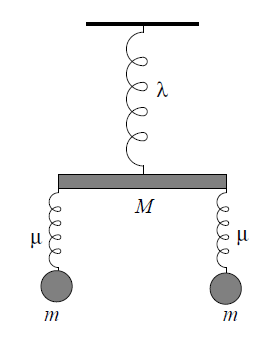
\includegraphics[scale=0.8]{2011P2Q7.PNG}
\end{figure}
\item Consider a system consisting of a heavy horizontal bar of mass $M$, from the ends of which two masses m hang on identical vertical springs, each with spring constant $\mu$ and equilibrium length $l$. The bar itself is suspended from a fixed point by a spring with spring constant $\lambda$ and equilibrium length $L$. (The bar is constrained to remain horizontal.) Define $q_1$, $q_2$ and $q_3$ to be the vertical displacements of, respectively, the bar and the two masses away from their equilibrium positions. Show that the relevant matrices $\mathbf{T}$ and $\mathbf{V}$ (as defined above) take the form
$$\mathbf{T}=\begin{pmatrix}M&0&0\\0&m&0\\0&0&m\\\end{pmatrix}, \quad\mathbf{V}=\begin{pmatrix}\frac{\lambda}{L}+\frac{2\mu}{l}&-\frac{\mu}{l}&-\frac{\mu}{l}\\-\frac{\mu}{l}&\frac{\mu}{l}&0\\-\frac{-\mu}{l}&0&\frac{\mu}{l}\\\end{pmatrix}$$
and hence construct the Lagrangian for this system.\hfill\textbf{[6]}
\item Hence for the case $M = 2$, $m = 1$, $\lambda= 4$, $\mu=1$, $L = 1$ and $l = 1$, derive the corresponding normal frequencies and normal modes.\hfill\textbf{[6]}
\item Give a brief geometrical description of each normal mode.\hfill\textbf{[3]}
\end{enumerate}
\end{qns}
\newpage
\begin{ans}\leavevmode
\begin{enumerate}[label=(\roman*)]
\item The Lagrangian of the system is the difference between the kinetic energy and the potential energy, i.e. $\mathcal{L}=\mathcal{T}-\mathcal{V}=\frac{1}{2}\mathbf{\dot{q}}^T\mathbf{T}\mathbf{\dot{q}}-\mathcal{V}(\mathbf{q})$. To extremize the Lagrangian, it has to satisfy the Euler-Lagrange equation
$$\frac{d}{dt}\frac{\partial\mathcal{L}}{\partial\mathbf{\dot{q}}}=\frac{\partial\mathcal{L}}{\partial\mathbf{q}}$$
At equilibrium, $\frac{\partial\mathcal{L}}{\partial\mathbf{q}}=\frac{\partial\mathcal{T}}{\partial\mathbf{q}}-\frac{\partial\mathcal{V}}{\partial\mathbf{q}}=0-0=0$. When we have a deviation $\Delta\mathbf{q}=(q_1,q_2,q_3)$ from $\mathbf{q_0}=\boldsymbol{0}$, then the Taylor expansion of $\mathcal{V}$ is
$$\mathcal{V}(\Delta\mathbf{q})=\mathcal{V}(\boldsymbol{0})+0+\frac{1}{2}(\Delta\mathbf{q}\cdot\boldsymbol{\nabla})^2\mathcal{V}+O(\Delta\mathbf{q})^3=\mathcal{V}(\boldsymbol{0})+\frac{1}{2}\begin{pmatrix}q_1&q_2&q_3\\\end{pmatrix}\begin{pmatrix}\frac{\partial^2\mathcal{V}}{\partial q_1^2}&\frac{\partial^2\mathcal{V}}{\partial q_1q_2}&\frac{\partial^2\mathcal{V}}{\partial q_1q_3}\\\frac{\partial^2\mathcal{V}}{\partial q_1q_2}&\frac{\partial^2\mathcal{V}}{\partial q_2^2}&\frac{\partial^2\mathcal{V}}{\partial q_2q_3}\\\frac{\partial^2\mathcal{V}}{\partial q_1q_3}&\frac{\partial^2\mathcal{V}}{\partial q_2q_3}&\frac{\partial^2\mathcal{V}}{\partial q_3^2}\\\end{pmatrix}\begin{pmatrix}q_1\\q_2\\q_3\\\end{pmatrix}+O(\Delta\mathbf{q}^2)$$
Then for small disturbances, we have $\mathcal{L}=\frac{1}{2}\mathbf{\dot{q}}^T\mathbf{T}\mathbf{\dot{q}}-\frac{1}{2}\mathbf{q}^T\mathbf{V}\mathbf{q}$, and so by the Euler-Lagrange equation, we have $\frac{d}{dt}(\mathbf{T\dot{q}})=-\mathbf{Vq}$. Let's assume $\mathbf{T}$ is independent of time. We look for solutions of the form $\mathbf{q}=\mathbf{a_n}e^{i\omega_nt}$ where $\mathbf{a_n}$ are the normal modes and $\omega_n$ are the normal frequencies, then we find the normal frequencies
$$-\omega^2\mathbf{Ta_n}=-\mathbf{Va_n}\implies\det|\mathbf{V}-\omega^2\mathbf{T}|=0$$
the normal modes are thus the corresponding eigenvectors for each normal frequency.
\item Define the $q_i$ coordinates relative to the equilibrium, then the kinetic energy is
$$\mathcal{T}=\frac{1}{2}M|\mathbf{\dot{q}_1}|^2+\frac{1}{2}m(|\mathbf{\dot{q}_2}|^2+|\mathbf{\dot{q}_3}|^2)=\frac{1}{2}\begin{pmatrix}\dot{q}_1&\dot{q}_2&\dot{q}_3\\\end{pmatrix}\begin{pmatrix}M&0&0\\0&m&0\\0&0&m\\\end{pmatrix}\begin{pmatrix}\dot{q}_1\\\dot{q}_2\\\dot{q}_3\\\end{pmatrix}$$
The potential energy is
$$\mathcal{V}=\frac{1}{2}\lambda q_1^2+\frac{1}{2}\mu(q_1-q_2)^2+\frac{1}{2}\mu(q_1-q_3)^2=\frac{1}{2}\begin{pmatrix}q_1&q_2&q_3\\\end{pmatrix}\begin{pmatrix}\lambda+2\mu&-\mu&-\mu\\-\mu&\mu&0\\-\mu&0&\mu\\\end{pmatrix}\begin{pmatrix}q_1\\q_2\\q_3\\\end{pmatrix}$$
We neglect gravity contributions to $\mathcal{V}$ since it merely redefines the equilibrium positions. The Lagrangian is thus
$$\mathcal{L}=\frac{1}{2}\begin{pmatrix}\dot{q}_1&\dot{q}_2&\dot{q}_3\\\end{pmatrix}\begin{pmatrix}M&0&0\\0&m&0\\0&0&m\\\end{pmatrix}\begin{pmatrix}\dot{q}_1\\\dot{q}_2\\\dot{q}_3\\\end{pmatrix}-\frac{1}{2}\begin{pmatrix}q_1&q_2&q_3\\\end{pmatrix}\begin{pmatrix}\lambda+2\mu&-\mu&-\mu\\-\mu&\mu&0\\-\mu&0&\mu\\\end{pmatrix}\begin{pmatrix}q_1\\q_2\\q_3\\\end{pmatrix}$$
\item With $M=2$, $m=1$, $\lambda=4$, $\mu=1$, $L=1$, $l=1$, solve for
$$0=\det|V-\omega^2T|=\det\begin{pmatrix}6-2\omega^2&-1&-1\\-1&1-\omega^2&0\\-1&0&1-\omega^2\\\end{pmatrix}=(1-\omega^2)((6-2\omega^2)(1-\omega^2)-2)=2(1-\omega^2)(\omega^4-4\omega^2+2)$$
with solutions $\omega^2=1$, $\omega^2=2\pm\sqrt{2}$, with respective normalized eigenvectors $\frac{1}{\sqrt{2}}(0,1,-1)^T$ and $\frac{1}{\sqrt{5\pm2\sqrt{2}}}(\mp\sqrt{2}-1,1,1)^T$.
\item 
\begin{itemize}
    \item $\omega^2=1$: the bar is stationary and the two masses are oscillating in anti-phase with equal amplitudes;
    \item $\omega^2=2+\sqrt{2}$: the two masses oscillate in phase, but the bar oscillate in anti-phase with relative amplitude $-\sqrt{2}-1$;
    \item $\omega^2=2-\sqrt{2}$: the two masses and the bar all oscillate in phase with relative amplitude $\sqrt{2}-1$;
\end{itemize}
\end{enumerate}
\end{ans}
\newpage
\begin{qns}[Group Theory]\leavevmode
\begin{enumerate}[label=(\roman*)]
\item Define the order $|G|$ of a finite group $G$ and the order of an element $g\in G$.\hfill\textbf{[2]}\\[5pt]
Consider the Cartesian product of two groups $G_1$ and $G_2$. This is the set $G_1\times G_2$ of all pairs ($g_1$, $g_2$) with the composition law
$$(g_1, g_2)(g'_1 , g′_2) ≡ (g_1g′_1, g_2g′_2 )$$
\item Show that $G_1\times G_2$ is a group. What is the order of the group?\hfill\textbf{[6]}
\item Consider the order 2 group $Z_2=\{e,w\}$.  Construct the multiplication table for the order 4 group $Z_2\times Z_2$.\hfill\textbf{[4]}
\item Now consider the order 4 cyclic group $Z_4 =\{e, a, a^2, a^3\}$. Show that the order 2 cyclic group $Z_2=\{e,a^2\}$ is a proper subgroup for $Z_4$. Prove there are no other proper subgroups for $Z_4$. Hence, show that $Z_2\times Z_2$ is not isomorphic to $Z_4$.\hfill\textbf{[8]}
\end{enumerate}
\end{qns}
\begin{ans}\leavevmode
\begin{enumerate}[label=(\roman*)]
\item The order of a group $G$ is the number of elements of $G$. If $G$ is a group and $g\in G$, the order of $g$ (denoted as $\ord(g)$) is the smallest $k\in\mathbb{N}$ s.t. $g^k=e$ where $e$ is the identity of $G$.
\item 
\begin{itemize}
    \item Closure: For $g_1,g_1'\in G_1$, $g_2,g_2'\in G_2$, $\implies$ $(g_1,g_2),(g_1',g_2)\in G_1\times G_2$. Since $G_1$ and $G_2$ are groups, $g_1,g_1'\in G_1\implies gg_1'\in G_1$, $g_2g_2'\in G_2\implies g_2g_2'\in G_2$, then we must have $(g_1g_1,g_2g_2')\in G_1\times G_2$.
    \item Identity: Let $e_1\in G_1$, $e_2\in G_2$ be identities, then 
    $$(e_1,e_2)(g_1,g_2)=(e_1g_1,e_2g_2)=(g_1,g_2)\in G_1\times G_2\implies (e_1,e_2)\in G_1\times G_2$$
    \item Associative: For $g_1,g_1',g_1''\in G_1$, $g_2,g_2',g_2''\in G_2$, then consider
    \begin{align}
    [(g_1,g_2)(g_1',g_2')](g_1'',g_2'')&=(g_1g_1',g_2g_2')(g_1'',g_2'')\nonumber\\&=(g_1g_1'g_1'',g_2g_2'g_2'')\nonumber\\&=(g_1,g_2)(g_1'g_1'',g_2',g_2'')\nonumber\\&=(g_1,g_2)[(g_1',g_2')(g_1'',g_2'')\nonumber
    \end{align}
    \item Inverse: Since $G_1$ and $G_2$ are groups, $g_1\in G_1\implies g_1^{-1}\in G_1$, $g_2\in G_2\implies g_2^{-1}\in G_2$, so 
    $$(g_1^{-1},g_2^{-1})(g_1,g_2)=(g_1^{-1}g_1,g_2^{-1}g_2)=(e_1,e_2)\in G_1\times G_2\implies(g_1^{-1},g_2^{-1})\in G_1\times G_2$$
    which is inverse for some $(g_1,g_2)\in G_1\times G_2$.
\end{itemize}
All the group axioms are satisfied. The order of $G_1\times G_2$ is $|G_1|\times|G_2|$.
\item Since the group $Z_2$ is order 2, then $w^2=e$. The group table of $Z_2\times Z_2$ is
$$\vbox{\tabskip0.5em\offinterlineskip
    \halign{\strut$#$\hfil\ \tabskip1em\vrule&&$#$\hfil\cr
      & (e,e)   & (e,w)  & (w,e) & (w,w)     \cr
    \noalign{\hrule}\vrule height 12pt width 0pt
    (e,e)   & (e,e)   & (e,w)  & (w,e) & (w,w)      \cr
    (e,w)   & (e,w)   & (e,e) & (w,w) & (w,e)      \cr
    (w,e) & (w,e) & (w,w) & (e,e) & (e,w)     \cr
    (w,w)  & (w,w)  &(w,e) & (e,w) & (e,e)     \cr
}}$$
\item The generators are $\langle e\rangle=\{e\}\implies\ord(e)=1$, $\langle a\rangle=\{a,a^2,a^3,e\}\implies\ord(a)=4$, $\langle a^2\rangle=\{a^2,e\}\implies\ord(a^2)=2$, $\langle a^3\rangle=\{a^3,a^2,a,e\}\implies\ord(a^3)=4$. The only order 2 group is the group $\langle a^2\rangle$. This is the cylic group $Z_2=\{e,a^2\}$ with group table
$$\vbox{\tabskip0.5em\offinterlineskip
    \halign{\strut$#$\hfil\ \tabskip1em\vrule&&$#$\hfil\cr
      & e&a^2     \cr
    \noalign{\hrule}\vrule height 12pt width 0pt
    e   & e&a^2      \cr
    a^2   & a^2&e      \cr
}}$$
\end{enumerate}
The group table illustrates closure. $Z_2$ inherits associativity from the parent group $Z_4$ and share the same identity $e$. For any $g\in Z_2$, the inverse is $g$ itself. $Z_2$ thus satisfies the axioms of a subgroup. Since $|Z_2|<|Z_4|$, $Z_2$ is a proper subgroup. But $\ord(a),\ord(a^3)=|Z_4|$ so $\langle a\rangle$, $\langle a^3\rangle$ are not proper subgroups. $\langle e\rangle$ is a trivial subgroup and by definition is not a proper subgroup.\\[5pt]
$Z_2\times Z_2$ has three order-two subgroups, namely 
$$\langle(w,w)\rangle,\quad\langle(e,w)\rangle,\quad\langle(w,e)\rangle$$
Hence the group $Z_2\times Z_2$ is not isomorphic to $Z_4$. For any isomorphism $\Phi:~G\rightarrow H$, elements must map to elements of the same order as if $g\mapsto h$, then 
$$h^{\ord(g)}=\Phi(g^{\ord(g)})=\Phi(e)=e$$
where we used the fact that $\Phi$ is a homomorphism. $\ord(h)$ must thus be a factor of $\ord(g)$. But $\Phi$ is also an isomorphism and hence invertible. By symmetry, $\ord(g)$ must also be a factor of $\ord(h)$. Thus, $\ord(g)=\ord(h)$. But, $\forall g\in Z_4$, the list of possible orders are $\{1,4,2,4\}$, whereas $\forall h\in Z_2\times Z_2$, the list of possible orders are $\{1,2,2,2\}$. The two groups are thus not isomorphic.
\end{ans}
\begin{qns}[Group Theory]\leavevmode
\begin{enumerate}[label=(\roman*)]
\item If $H$ and $K$ are subgroups of $G$, show that the intersection $H\cup K$ is also a group.\hfill\textbf{[6]}
\item Consider $D_3$, the group of symmetries of the equilateral triangle. $D_3$ has six elements: the identity ($I$); two rotations ($A$,$B$); and three reflections ($C$,$D$,$E$). Explain their geometrical action on the equilateral triangle. Construct the multiplication table for $D_3$. Is this group abelian?\hfill\textbf{[9]}
\item How many order 2 subgroups are there in $D_3$? List them. Are they normal subgroups of $D_3$? Justify your conclusion. Finally, show by explicit construction that the union of two order 2 subgroups of $D_3$ does not form a group.\hfill\textbf{[5]}
\end{enumerate}
\end{qns}
\begin{ans}\leavevmode
\begin{enumerate}[label=(\roman*)]
\item Check axioms of a group:
\begin{itemize}
    \item Closure: If $g_1,g_2\in H\cap K$, $g_1g_2\in H\cap K$.
    \item Identity: $H,K\leq G$ $\implies$ $e\in H$, $e\in K$ $\implies$ $e\in H\cap K$.
    \item Associativity: $H\cap K$ inherits associativity from $H,K$.
    \item Inverse: $H,K\leq G$, $g_2,g_1\in H\cap K$ $\implies$ $g_1^{-1},g_2^{-1}\in H\cap K$.
\end{itemize}
\item Let the 3 vertices of a triangle be $(a,b,c)$, then the mappings are:
$$I:~(a,b,c)\mapsto(a,b,c),\quad A:~(a,b,c)\mapsto(b,c,a),\quad B:~(a,b,c)\mapsto(c,a,b)$$
$$C:~(a,b,c)\mapsto(a,c,b),\quad D:~(a,b,c)\mapsto(c,b,a),\quad E:~(a,b,c)\mapsto(b,a,c)$$
Since $A$, $B$ are rotations, $A^3=B^3=I$. Also, $A$ and $B$ are rotations in the opposite directions and so $A^{-1}=B$ and $B^{-1}=A$. Since $C$, $D$ and $E$ are reflections, then $C^2=D^2=E^2=I$. We can thus work out $AC=D$, $AD=E$, $AE=C$ and similar relations. The group table of $D_3$ is thus
$$\vbox{\tabskip0.5em\offinterlineskip
    \halign{\strut$#$\hfil\ \tabskip1em\vrule&&$#$\hfil\cr
      & I   & A  & B & C & D &E     \cr
    \noalign{\hrule}\vrule height 12pt width 0pt
    I   & I   & A  & B & C & D &E   \cr
    A   & A & B &I &D &E &C  \cr
    B & B & I & A & E &C &D \cr
    C & C &E & D& I & B &A     \cr
    D& D &C&E&A&I&B\cr
    E& E &D &C &B &A&I\cr
}}$$
The group table is not symmetric on the main diagonal, hence $D_3$ is not abelian (it is also the smallest non-abelian subgroup).
\item Since the reflections have order 2, the order 2 subgroups in $D_3$ are 
$$\{I,C\},\quad\{I,D\},\quad\{I,E\}$$
All 3 subgroups are not normal in $D_3$ as $\{C,D,E\}$ form a conjugacy class. None of the above are constructed from the union of entire conjugacy classes. $\{I,C\}\cup\{I,D\}=\{I,C,D\}$ is not a group as it is not closed. For instance, $CD=B\notin\{I,C,D\}$.
\end{enumerate}
\end{ans}
\newpage
\begin{qns}[Representation Theory]\leavevmode
[In this question, you may state without proof any theorems you use.]
\begin{enumerate}[label=(\roman*)]
\item Suppose $G_1$ and $G_2$ are groups, and $D$ is a mapping $D : G_1\rightarrow G_2$. Give the definition for the map D to be a homomorphism. What is the kernel of $D$, $\ker(D)$?\hfill\textbf{[2]}\\[5pt]
Let $S_3 = \{e, x, y, y^2, xy, xy^2\}$ be the $n = 3$ symmetric group with
$$x^2=y^3=e,\quad yx=xy^2,\quad y^2x=xy$$
\item Verify by explicit calculation that, with $z=e^{2\pi i/3}$,
\begin{align}
    &R(x)=\begin{pmatrix}0&1\\1&0\\\end{pmatrix},\quad R(y)=\begin{pmatrix}z&0\\0&z^2\\\end{pmatrix},\quad R(y^2)=\begin{pmatrix}z^2&0\\0&z\\\end{pmatrix}\nonumber\\&R(xy)=\begin{pmatrix}0&z^2\\z&0\\\end{pmatrix},\quad R(xy^2)=\begin{pmatrix}0&z\\z^2&0\\\end{pmatrix}\tag{*}
\end{align}
is a two-dimensional complex representation of $S_3$. You can assume without proof that (*) is an irreducible representation.\hfill\textbf{[7]}
\item Given that the trivial representation of $S_3$ is the one-dimensional complex representation $T(s) = 1$ where $s\in S_3$, find the non-trivial one-dimensional complex representation $U:S_3\rightarrow\mathbb{C}^1$. What is $\Ker(U)$? Is $U$ a faithful representation?\hfill\textbf{[8]}
\item Finally, given these results, deduce the number of conjugacy classes in $S_3$.\hfill\textbf{[3]}
\end{enumerate}
\end{qns}
\begin{ans}\leavevmode
\begin{enumerate}[label=(\roman*)]
\item If $G_1$ and $G_2$ are groups then a function $D:~ G_1\rightarrow G_2$ is called a group homomorphism, if $\forall a,b\in G_1$, we have $D(a\cdot_{G_1} b)=D(a)\cdot_{G_2}D(b)$. For the group homomorphism $D:~G_1\rightarrow G_2$, the kernel of $D$ is $\Ker(D):=\{h\in G_1|D(h)=e_{G_2}\text{  for some } h\in G_1\}$.
\item Since $z=e^{2\pi i/3}$, then $z^3=1$. Define $R(e):=\begin{pmatrix}1&0\\0&1\\\end{pmatrix}$. Then, since $R$ is a representation, $R$ is a homomorphism. Verify the group table of $S_3$.
$$R(x^2)=R(x)R(x)=\begin{pmatrix}0&1\\1&0\\\end{pmatrix}\begin{pmatrix}0&1\\1&0\\\end{pmatrix}=\begin{pmatrix}1&0\\0&1\\\end{pmatrix}=R(e)\implies x^2=e$$
$$R(y^3)=R(y)R(y)R(y)=\begin{pmatrix}z&0\\0&z^2\\\end{pmatrix}\begin{pmatrix}z&0\\0&z^2\\\end{pmatrix}\begin{pmatrix}z&0\\0&z^2\\\end{pmatrix}=\begin{pmatrix}z^2&0\\0&z^4\\\end{pmatrix}\begin{pmatrix}z&0\\0&z^2\\\end{pmatrix}=R(e)\implies y^3=e$$
$$R(yx)=R(y)R(x)=\begin{pmatrix}z&0\\0&z^2\\\end{pmatrix}\begin{pmatrix}0&1\\1&0\\\end{pmatrix}=\begin{pmatrix}0&z\\z^2&0\\\end{pmatrix}=\begin{pmatrix}0&1\\1&0\\\end{pmatrix}\begin{pmatrix}z^2&0\\0&z^4\\\end{pmatrix}=R(x)R(y^2)=R(xy^2)$$
$$R(y^2x)=R(y^2)R(x)=\begin{pmatrix}z^2&0\\0&z^4\\\end{pmatrix}\begin{pmatrix}0&1\\1&0\\\end{pmatrix}=\begin{pmatrix}0&z^2\\z&0\\\end{pmatrix}=\begin{pmatrix}0&1\\1&0\\\end{pmatrix}\begin{pmatrix}z&0\\0&z^2\\\end{pmatrix}=R(x)R(y)=R(xy)$$
The last two implies $yx=xy^2$ and $y^2x=xy$ respectively.
\item Let $x=a\in\mathbb{C}^1$, $y=b\in\mathbb{C}^1$, then the group table of $S^3$ gives $a=-1$, $b=1$. So the character of $U$ is the list of trace of $U(s)$ for $s\in S_3$. Since $\mathbb{C}^1$ is a number, its trace is itself, so
$$\chi(U)=\{e=1,x=-1,y=1,y^2=1,xy=-1,xy^2=-1\}$$
which is orthogonal to $\chi(T)=\{1,1,1,1,1,1\}$ (trivial rep) and 
$$\chi(D)=\{\Tr(R(e)),\Tr(R(x)),\Tr(R(y)),\Tr(R(y^2)),\Tr(R(xy)),\Tr(R(xy^2))\}=\{2,0,-1,-1,0,0\}$$
where we used the roots identity $1+z+z^2=0$, for $z=e^{i2\pi/3}$. From part (i), $\Ker(U)=\{s\in S_3|U(s)=1\}=\{e,y,y^2\}\neq\{0\}$, which is non-trivial, hence not a  faithful representation
\item Since the number of irreducible representations is the number of conjugacy classes and the sum of squares of irreducible representations is the order of the group, we have
$$|S_3|=3!=6=1^2+1^2+2^2$$
where we have two one-dimensional representations $T,U$ and one two-dimensional representation $D$. Hence, there is exactly 3 conjugacy classes.


\end{enumerate}

\end{ans}
\newpage
\section{2012}
\subsection{Paper 1}
\begin{qns}[Vector Calculus]\leavevmode
\begin{enumerate}[label=(\alph*)]
    \item Let $\mathbf{F}$ be a vector field and $\mathbf{a}$ be an arbitrary constant vector. Show that \hfill \textbf{[4]}
$$\boldsymbol{\nabla}\times(\mathbf{a}\times\mathbf{F})=\mathbf{a}(\boldsymbol{\nabla}\cdot\mathbf{F})-(\mathbf{a}\cdot\boldsymbol{\nabla})\mathbf{F}$$
\item State Stokes' Theorem.\hfill \textbf{[2]}
\item By applying it to the above identity, show that 
$$\int_C d\mathbf{l}\times\mathbf{F}=\int_S(d\mathbf{S}\times\boldsymbol{\nabla})\times\mathbf{F}$$
for any closed curve $C$ that bounds a surface $S$.\hfill \textbf{[8]}
\item Verify this identity for the case where $C$ is a square path starting at (0,0,0), then progressing in a straight line to (0,1,0), then to (1,1,0), then to (1,0,0) and finally back to the origin with $\mathbf{F}=\mathbf{r}$, where $\mathbf{r}=(x,y,z)$.\hfill \textbf{[6]}
\end{enumerate}
\end{qns}
\begin{ans}\leavevmode
\begin{enumerate}[label=(\alph*)]
    \item Use suffix notation. LHS is $\epsilon_{kij}\epsilon_{pqj}\partial_ia_pF_q=\partial_ia_kF_i-\partial_ia_iF_k=a_k(\boldsymbol{\nabla}\cdot\mathbf{F})-(\mathbf{a}\cdot\boldsymbol{\nabla})F_k$, as desired.
    \item Let $\mathbf{F}=\mathbf{F}(\mathbf{x})$ be a continuously differentiable vector field, and let surface $S$ be orientable, piecewise regular with piecewise smooth boundary $\partial S$, then Stokes' theorem states that
$$\int_S(\boldsymbol{\nabla}\times\mathbf{F})\cdot d\mathbf{S}=\oint_{\partial S}\mathbf{F}\cdot d\mathbf{x}$$
    \item Apply Stokes' theorem to part (a)'s result:
$$\oint_C(\mathbf{a}\times\mathbf{F})\cdot d\mathbf{l}=\int_S\bigg(\boldsymbol{\nabla}\times(\mathbf{a}\times\mathbf{F})\bigg)\cdot d\mathbf{S}=\int_S(d\mathbf{S}\times\boldsymbol{\nabla})\cdot(\mathbf{a}\times\mathbf{F})=-\int_S((d\mathbf{S}\times\boldsymbol{\nabla})\times\mathbf{F})\cdot \mathbf{a}$$
where we used $\epsilon_{ijk}\partial_i(\epsilon_{pqj}a_pF_q)dS_k=(\epsilon_{kij}dS_k\partial_i)\epsilon_{pqj}a_pF_q= -\epsilon_{jqp}(\epsilon_{kij}dS_k\partial_i)F_qa_p$, but the LHS is also $-\oint_C( d\mathbf{l}\times\mathbf{F})\cdot\mathbf{a}$. Putting everything to one side
$$\mathbf{a}\cdot\bigg(\oint_C(d\mathbf{l}\times\mathbf{F})-\int_S(d\mathbf{S}\times\boldsymbol{\nabla})\times\mathbf{F}\bigg)=0$$
where $\mathbf{a}$ is a constant vector and can be pulled out of the integral. $\mathbf{a}$ is also arbitrary, so whatever is dotted with $\mathbf{a}$ must be a zero vector. The result follows.
\item Let $d\mathbf{S}=(0,0,-dxdy)$, then $d\mathbf{S}\times\boldsymbol{\nabla}=(-\partial_y,\partial x,0)dxdy$ and so $\int_S(d\mathbf{S}\times\boldsymbol{\nabla})\times\mathbf{F}=(0,0,2)$. For $C$, we segment into four segments: 
\begin{itemize}
    \item $C_1$ where $d\mathbf{l}=(0,dt,0)$ with $y=t$, $0\leq t\leq 1$;
    \item $C_2$ where $d\mathbf{l}=(dt,0,0)$ with $x=t$, $0\leq t\leq 1$ and $y=1$;
    \item $C_3$ where $d\mathbf{l}=(0,-dt,0)$ with $x=1$, $y=1-t$, $0\leq t\leq 1$;
    \item $C_4$ where $d\mathbf{l}=(-dt,0,0)$ with $x=1-t$.
\end{itemize}
The line integral gives the same result, with only the term from $C_2$ and $C_3$ contributes.
$$\int_Cd\mathbf{l}\times\mathbf{F}=\bigg(\int_0^1dt+\int_0^1dt\bigg)\mathbf{\hat{z}}=2\mathbf{\hat{z}}$$
$$\int_S(d\mathbf{S}\times\boldsymbol{\nabla})\times\mathbf{F}=\int_0^1\int_0^12\mathbf{\hat{z}}dxdy=2\mathbf{\hat{z}}$$
\end{enumerate}
\end{ans}
\newpage
\begin{qns}[Laplace's Equation]
The number density of neutrons $n(\mathbf{r},t)$ in a lump of Uranium is determined by the PDE
$$\nabla^2n=\frac{\partial n}{\partial t}-\lambda n$$
where $\nabla^2$ is the Laplacian operator, $\mathbf{r}$ is the position vector, $t$ is the time and $\lambda$ is a constant.
\begin{enumerate}[label=(\alph*)]
\item Suppose the lump of Uranium is a sphere of radius $a$, and the density of the neutrons is spherically symmetric. Furthermore, suppose this equation can be solved by the method of separation of variables so that
$$n=R(r)T(t)$$
where $r$ is the distance from the centre of the sphere. Find two ordinary differential equations for $R(r)$ and $T(t)$.\hfill \textbf{[4]}
\item Suppose that the density of neutrons is never zero, except at the surface of the sphere, and finite everywhere inside. Find $n(\mathbf{r},t)$.\hfill \textbf{[8]}
\item Show that the concentration of neutrons will grow as a function of time provided that\hfill \textbf{[8]} $$\lambda>\pi^2/a^2$$
\end{enumerate}
[Hint: To find $R(r)$, substitute $R(r)=r^pf(r)$ for some $p$.]
\end{qns}
\begin{ans}\leavevmode
\begin{enumerate}[label=(\alph*)]
    \item Use separation of variables $n(r,t)=R(r)T(t)$, then
$$\frac{1}{r^2R}\frac{d}{dr}r^2\frac{dR}{dr}=\frac{1}{T}\frac{dT}{dt}-\lambda=-b$$
which gives two ODE
\begin{equation}
\frac{dT}{dt}=(\lambda-b)T\tag{time}
\end{equation} 
\begin{equation}
\frac{d}{dr}r^2\frac{dR}{dr}=-br^2R\tag{radial}
\end{equation}
\item Guessing the form $R(r)=r^pf(r)$, we have
$$r^{p+2}f''(r)+(r^{p+1}+(p+2)r^{p+1})f'(r)+p(p+1)r^p-br^{2+p}f(r)=0$$
Choosing $p=-1$, we have $f''(r)r=-brf(r)$ and so
$$R(r)=\frac{1}{r}(Ae^{\sqrt{-b}r}+Be^{-\sqrt{-b}r})$$
For $R$ to be finite everywhere inside, we require $A=-B$. $r=a$ is also the first zero where $R(r=a)=0$. This requires $e^{2\sqrt{-b}a}=1$ and so 
$$R(r)=\frac{A\sin(\pi r/a)}{r}$$
for $n=1$ to be the first zero and that $n=\frac{\pi}{a}$. Similarly, $T(t)=e^{(\lambda-\pi^2/a^2)t}$. Finally,
$$n(r,t)=\frac{A}{r}\sin\frac{\pi r}{a}e^{(\lambda-\frac{\pi^2}{a^2})t}$$
\item $T(t)=e^{(\lambda-\pi^2/a^2)t}$ diverges if $\lambda>\pi^2/a^2$
\end{enumerate}
\end{ans}
\newpage
\begin{qns}[Green's Functions]\leavevmode
\begin{enumerate}[label=(\alph*)]
\item Find the general solution $y(x)$ to the homogeneous second-order linear differential equation 

\hfill \textbf{[6]}
$$\frac{d^2y}{dx^2}+\frac{3}{x}\frac{dy}{dx}+\frac{y}{x^2}=0$$
\item Construct the Green's function for this equation in the region $0\leq x<\infty$, which satisfies
$$\frac{d^2}{dx^2}G(x,\xi)+\frac{3}{x}\frac{d}{dx}G(x,\xi)+\frac{1}{x^2}G(x,\xi)=\delta(x-\xi)$$
subject to the boundary conditions $G(0,\xi)=\frac{d}{dx}G(0,\xi)=0$, where $\delta(x-\xi)$ is the Dirac delta function. \hfill \textbf{[8]}
\item Use your Green's function to solve the differential equation
$$\frac{d^2y}{dx^2}+\frac{3}{x}\frac{dy}{dx}+\frac{y}{x^2}=x$$
for $x\geq0$, subject to the boundary conditions $y(0)=y'(0)=0$.\hfill \textbf{[6]}
\end{enumerate}
\end{qns}
\begin{ans}\leavevmode
\begin{enumerate}[label=(\alph*)]
\item The general solution to the homogeneous equation is $y=c_1x^{-1}+c_2x^{-1}\ln(x)$, where we substitute $y=x^r$ for $r\in\mathbb{R}$ to obtain quadratic equation, i.e. $r^2+2r+1=0$.
\item The corresponding Green's function must satisfy the given DE and the b.c.s $G(0,\xi)=G'(0,\xi)=0$. Using the homogeneous solutions in part (a), we guess the Green's function $G(x,\xi)$ to be
$$G(x,\xi)=
\left\{
        \begin{array}{ll}
      (A(\xi)+B(\xi)\ln(x))x^{-1}& 0\leq x<\xi<\infty \\
      (C(\xi)+D(\xi)\ln(x))x^{-1} & 0\leq\xi<x<\infty
        \end{array}
    \right.$$
Since $G(0,\xi)=\frac{\partial G}{\partial x}(0,\xi)=0$, we must have $A=B=0$. Integrating the DE over a small infinitesimal region at $x=\xi$, one obtains the jump condition $[\frac{\partial G}{\partial x}]_-^+=1$. $G$ must be continuous everywhere, including $x=\xi$. Otherwise, $G''\propto\delta'(x-\xi)$ which is a contradiction. Imposing the jump and continuity condition respectively gives
$$\frac{\partial G}{\partial x}=-x^{-2}(C(\xi)+D(\xi)\ln(x))+D(\xi)x^{-2}\implies D-C-D\ln\xi=\xi$$
$$C(\xi)+D(\xi)\ln(\xi)=0$$
Both requires $D=\xi^2$ and $C=-\xi^2\ln\xi$. Hence, $$G(x,\xi)=
\left\{
        \begin{array}{ll}
      0& 0\leq x<\xi<\infty \\
      -\frac{\xi^2}{x}\ln(\xi/x) & 0\leq\xi<x<\infty
        \end{array}
    \right.$$
\item The solution for the differential equation will be
$$y=\int_0^\xi G(x,\xi)f(\xi)d\xi=-\int_0^\xi\frac{\xi^2}{x}\ln(\xi/x)\xi d\xi=-x^3\int_0^1u^3\ln(u)du=\frac{1}{16}x^3$$
where we used the substitution $u=\xi/x$ and integrated by parts. By construction, $y$ obeys the desired boundary conditions.
\end{enumerate}
\end{ans}
\newpage
\begin{qns}[Fourier Transform]\leavevmode
\begin{enumerate}[label=(\alph*)]
\item Calculate the Fourier transform of the function
$$f(x)=e^{-\lambda x^2}$$
where $\lambda$ is a positive constant.\hfill \textbf{[5]}
\item Consider the partial differential equation for $\psi(x,t)$
$$\frac{\partial^2\psi}{\partial x^2}=\frac{\partial\psi}{\partial t}$$
Find the ordinary differential equation that
$$\tilde{\psi}(k,t)=\int_{-\infty}^\infty\psi(x,t)e^{-ikx}dx$$
obeys. \hfill \textbf{[5]}
\item Find $\tilde{\psi}(k,t)$ given $\psi(x,0)=e^{-\lambda x^2}$.\hfill \textbf{[5]}
\item Hence find $\psi(x,t)$ for $t>0$.\hfill \textbf{[5]}
\begin{mdframed}
\textcolor{darkblue}{Hint: You may find the following relation 
$$\int_{-\infty}^\infty e^{-\lambda(x+i\alpha)^2}dx=\sqrt{\frac{\pi}{\lambda}}$$
for $\alpha$ and $\lambda$ real constants and $\lambda<0$.}
\end{mdframed}
\end{enumerate}
\end{qns}
\begin{ans}\begin{enumerate}[label=(\alph*)]
\item Evaluate the Fourier Transform
$$\tilde{f}(k)=\int_{-\infty}^\infty e^{-\lambda x^2}e^{-ikx}dx=\int_{-\infty}^\infty e^{-\lambda(x^2+(ikx/\lambda))}dx=\int_{-\infty}^\infty e^{-\lambda(x+\frac{ik}{2\lambda})^2}e^{-\lambda\frac{k^2}{4\lambda^2}}dx=e^{-\frac{k^2}{4\lambda}}\sqrt{\frac{\pi}{\lambda}}$$
\item Taking the Fourier Transform for the PDE w.r.t $x$,
$$\int_{-\infty}^\infty\frac{\partial^2\psi}{\partial x^2}e^{-ikx}dx=\frac{\partial}{\partial t}\int_{-\infty}^\infty\psi e^{-ikx}dx$$
Integrating the LHS twice such that $[\frac{\partial\psi}{\partial x}e^{-ikx}]_{-\infty}^\infty$, $[ik\psi e^{-ikx}]_{-\infty}^\infty$ to be both zero, we have $\frac{\partial\tilde{\psi}}{\partial t}=-k^2\tilde{\psi}$.
\item $\tilde{\psi}(k,t)=\tilde{\psi}(k,0)e^{-k^2t}$ will be the solution. We have
$$\tilde{\psi}(k,t)=\tilde{\psi}(k,0)e^{-k^2t}=\mathcal{F}[\psi(x,0)]e^{-k^2t}=\sqrt{\frac{\pi}{\lambda}}e^{-k^2/4\lambda}e^{-k^2t}$$
\item Invert the answer from part (c),
$$\psi(x,t)=\frac{1}{2\pi}\int_{-\infty}^\infty\tilde{\psi}(k,t)e^{ikx}dk=\frac{1}{2\pi}\int_{-\infty}^\infty\sqrt{\frac{\pi}{\lambda}}e^{-k^2/4\lambda}e^{-k^2t}e^{ikx}dk$$
We substitute $\beta=t+\frac{1}{4\lambda}$ such that we can complete the square.
$$\psi(x,t)=\frac{1}{2\sqrt{\pi\lambda}}\int_{-\infty}^{\infty}\exp\bigg(-\beta\bigg[\bigg(k-\frac{ix}{2\beta}\bigg)^2+\frac{x^2}{4\beta^2}\bigg]\bigg)dk=\frac{1}{2\sqrt{\pi\lambda}}e^{-x^2/4\beta}\sqrt{\frac{\pi}{\beta}}=\frac{1}{2\sqrt{\lambda t+0.25}}e^{-x^2/(4t+\lambda^{-1})}$$
\end{enumerate}
\end{ans}
\newpage
\begin{qns}[Linear Algebra]\leavevmode
\begin{enumerate}[label=(\roman*)]
\item Show that an $n\times n$ matrix $A$ is diagonalisable if it has $n$ linearly independent eigenvectors. Show that if $A$ is diagonalisable, then so is $B = P^{−1}AP$, where $P$ is an $n\times n$ matrix and $P^{−1}$ is its inverse.\hfill \textbf{[6]}
\item Let $\lambda_i$ (with $i=1,2,...,n$) be the eigenvalues of an $n\times n$ Hermitian matrix $A$.
\begin{enumerate}[label=(\alph*)]
\item Show that\hfill \textbf{[6]}
$$\Tr(A^k)=\sum_{i=1}^n\lambda_i^k\text{ and } \det(A^k)=\prod_{i=1}^n\lambda_i^k$$
for all positive integers $k$.
\item Show that \hfill \textbf{[4]}
$$\det(\exp(A))=\exp(\Tr(A))$$
\item If $A^2=A$, prove that either (i) $\det(A)=1$ and $\Tr(A)=n$ or (ii) $\det(A)=0$ and $\Tr(A)=m<n$, where $m$ is an integer. \hfill \textbf{[4]}
\end{enumerate}
\end{enumerate}
\end{qns}
\begin{ans}\leavevmode
\begin{enumerate}[label=(\roman*)]
\item Let the normalized eigenvectors of $A$ be $\{\mathbf{e_i}\}$, then $R=(\mathbf{e_1},\mathbf{e_2},...)$ such that $R^{-1}=(\mathbf{b_1}^T,\mathbf{b_2}^T,...)^T$ where $\mathbf{b_i}\cdot\mathbf{e_j}=\delta_{ij}$, then
$$R^{-1}AR=(\mathbf{b_1}^T,\mathbf{b_2}^T,\dots)^T(\lambda_1\mathbf{e_1},\lambda_2\mathbf{e_2},\dots)^T=\diag(\lambda_1,\lambda_2,...,\lambda_n)$$
Indeed, $R$ diagonalizes $A$. Now if $A$ is diagonalizable, then to diagonalize $B=P^{-1}AP$, we require the matrix $Q=P^{-1}R$:
$$Q^{-1}BQ=(P^{-1}R)^{-1}(P^{-1}AP)(P^{-1}R)=R^{-1}PP^{-1}APP^{-1}R=R^{-1}AR=\diag(\lambda_1,...,\lambda_n)$$
so $Q$ diagonalizes $B$.
\item 
\begin{enumerate}[label=(\alph*)]
\item To show $\Tr(A^k)=\sum_{i=1}^n\lambda_i^k$, we require $\Tr(A^k)=\Tr((\diag(\lambda_1,...,\lambda_n))^k)$. From part (i), in order to diagonalize $A$, it must have $n$ linearly independent eigenvectors. This is true since the eigenvectors of a Hermitian matrix are orthogonal, i.e. consider $A\mathbf{e_i}=\lambda_i\mathbf{e_i}$, then
$$\lambda_i\mathbf{e_j}^\dag\mathbf{e_i}=\mathbf{e_j}^\dag A\mathbf{e_i}=(A^\dag\mathbf{e_j})^\dag\mathbf{e_i}=(A\mathbf{e_j})^\dag\mathbf{e_i}=(\lambda_j\mathbf{e_j})^\dag\mathbf{e_i}=\lambda_j^*\mathbf{e_j}^\dag\mathbf{e_i}$$
For $\lambda_j^*\neq\lambda_i$, then $\mathbf{e_j}^\dag\mathbf{e_i}=0$ and hence eigenvectors of different eigenvalues are pairwise orthogonal.\\[5pt] 
We can thus find a unitary matrix $R$ that diagonalizes $A$, i.e. $\Lambda:=\diag(\lambda_1,...,\lambda_n)=R^\dag AR$. Then,
$$\Tr(A^k)=\Tr((R\Lambda R^\dag)^k)=\Tr(R\Lambda^kR^\dag)=\Tr(\Lambda^kRR^\dag)=\Tr(\Lambda^k)=\sum_{i=1}^n\lambda_i^k$$
$$\det(A^k)=\det((R\Lambda R^\dag)^k)=\det(R\Lambda^kR^\dag)=\det(\Lambda^k)\det(RR^\dag)=\det(\diag(\lambda_1^k,...,\lambda_n^k))=\prod_{i=1}^n\lambda_i^k$$
\item By definition of exponential of a matrix, we have $\exp^B=\sum_{n=0}^\infty\frac{1}{n!}B^n$. Then, $\det(\exp(A))$ is
$$\det\bigg(\sum_{n=0}^\infty\frac{1}{n!}(R^\dag\Lambda R)^n\bigg)=\det\bigg(R^\dag\sum_{n=0}^\infty\frac{1}{n!}\Lambda^nR\bigg)=\det\bigg(\sum_{n=0}^\infty\frac{1}{N!}\Lambda^n\bigg)=\prod_{i=1}^ne^{\lambda_i}=e^{\sum_{i=1}^n\lambda_i}=e^{\Tr(A)}$$
\item If $A^2=A$, each eigenvalue must be a square of itself, and hence can only be zero or 1. Also, $A^2=A\implies\det(A)=\det(A^2)=\det(A)\det(A)\implies\det(A)(\det(A)-1)=0$. If $\det(A)=1$, then $\Tr(A)=n$. Similarly, if $\det(A)=0$, then $\Tr(A)<n$.
\end{enumerate}
\end{enumerate}
\end{ans}
\newpage
\begin{qns}[Linear Algebra]\leavevmode
\begin{enumerate}[label=(\roman*)]
\item Let $A$ be a complex $n\times n$ matrix, and define
$$H=\frac{1}{2}(A+A^\dag)\text{ and }S=\frac{1}{2i}(A-A^\dag)$$
Let $\lambda$ be an eigenvalue of $A$, and $x$ be the corresponding unit-normalized eigenvector.
\begin{enumerate}[label=(\alph*)]
\item Show that $\lambda=x^\dag Hx+ix^\dag Sx$.\hfill \textbf{[4]}
\item Show that the real part of $\lambda$ is given by $\text{Re}(\lambda)=x^\dag Hx$ and the imaginary part is given by $\text{Im}(\lambda)=x^\dag Sx$.\hfill \textbf{[4]}
\end{enumerate}
\item Let $B$ be a Hermitian $n\times n$ matrix with $n$ distinct (real) eigenvalues $\lambda_i$.
\begin{enumerate}[label=(\alph*)]
\item Show that the corresponding normalised eigenvectors $x_i$ satisfy
$$x_i^\dag x_j=\delta_{ij}$$
and therefore form an orthonormal basis, $\{x_i:i=1,2,...,n\}$.\hfill \textbf{[6]}
\item Now, consider
$$\beta=(Bv-av)^\dag(Bv-bv)$$
where $v$ is an arbitrary vector, while $a$ and $b$ are real constants with $a < b$. By expanding $v$ in terms of the eigenvectors $x_i$, show that $\beta>0$ if no eigenvalue lies in the interval $[a, b]$.\hfill \textbf{[6]}
\end{enumerate}
\end{enumerate}
\end{qns}
\begin{ans}\leavevmode
\begin{enumerate}[label=(\roman*)]
\item 
\begin{enumerate}[label=(\alph*)]
\item We have $Ax=\lambda x$ and $x^\dag x=1$, so
$$x^\dag Hx+ix^\dag Sx=\frac{1}{2}[x^\dag Ax+x^\dag A^\dag x]+\frac{1}{2}[x^\dag Ax-x^\dag A^\dag x]=x^\dag Ax=\lambda$$
\item Take the conjugate transpose,
$$\lambda^*=(x^\dag Hx+ix^\dag Sx)^\dag=x^\dag Hx-ix^\dag Sx$$ Add and subtract gives 
$$2x^\dag Hx=\lambda+\lambda^*=2\text{Re}[\lambda],\quad 2ix^\dag Sx=\lambda-\lambda^*=2i\text{Im}[\lambda]\implies \text{Re}[\lambda]=x^\dag Hx,~\text{Im}[\lambda]=x^\dag Sx$$
\end{enumerate}
\item
\begin{enumerate}[label=(\alph*)]
\item Consider
$$\lambda_jx_i^\dag x_j=x_i^\dag Bx_j=(Bx_i)^\dag x_j=\lambda_i^* x_i^\dag x_j$$
where $B$ is Hermitian. If $i\neq j$, then we are given $\lambda_i\neq\lambda_j=\lambda_j^*$, and hence $x_i^\dag x_j=0$. Further, given $x_i^\dag x_i=1$ $\forall i$, then $x_i^\dag x_j=\delta_{ij}$.
\item Write $v=\sum_i\alpha_ix_i$, then 
\begin{align}
\beta=(Bv-av)^\dag(Bv-bv)&=\sum_i(\lambda_i-a)^\dag(\alpha_ix_i)^\dag\sum_j(\lambda_j-b)\alpha_jx_j\nonumber\\&=\sum_i\sum_j\alpha_i^*\alpha_j(\lambda_i-a)(\lambda_j-b)\delta_{ij}\nonumber\\&=\sum_i|\alpha_i|^2(\lambda_i-a)(\lambda_i-b)\nonumber
\end{align}
If $\lambda_i\in[a,b]$, then $(\lambda_i-a)>0$ and $(\lambda_i-b)<0$ and so $\beta<0$. For $\beta>0$ to be true, $\lambda_i\notin[a,b]$.
\end{enumerate}
\end{enumerate}
\end{ans}
\newpage
\begin{qns}[Cauchy-Riemann]\leavevmode
\begin{enumerate}[label=(\roman*)]
\item Two-dimensional fluid flow can be described by a complex potential
$$f(z)=u(x,y)+iv(x,y)$$
where $z=x+iy$. Let the fluid velocity be $\mathbf{V}=\boldsymbol{\nabla}u$. If $f(z)$ is analytic, show that
\begin{enumerate}[label=(\alph*)]
\item  $\boldsymbol{\nabla}\cdot\mathbf{V}=0$,\hfill \textbf{[4]}
\item $\frac{df}{dz}=V_x-iV_y$.\hfill \textbf{[4]}
\end{enumerate}
[You may assume the Cauchy-Riemann equations without proof.]
\item Consider the Gamma function
$$\Gamma(z)=\int_0^\infty t^{z-1}e^{-t}dt, \text{ for }\text{Re}(z)>0$$
\begin{enumerate}[label=(\alph*)]
\item Using integration by parts, derive the recursion relation 
\begin{equation}
    \Gamma(z+1)=z\Gamma(z)\tag{*}
\end{equation}
Also show that $\Gamma(1)=1$.\hfill \textbf{[4]}
\item Assuming that $(*)$ holds $\forall z\in\mathbb{C}$, show that $\Gamma(z)$ has simple poles at all non-positive integers. Compute their residues.\hfill \textbf{[8]}
\end{enumerate}
\end{enumerate}
\end{qns}
\begin{ans}\leavevmode
\begin{enumerate}[label=(\roman*)]
\item 
\begin{enumerate}[label=(\alph*)]
\item If $f(z)$ is analytic, then $f(z)$ satisfies the Cauchy-Riemann equations $\frac{\partial u}{\partial x}=\frac{\partial v}{\partial y}$ and $\frac{\partial u}{\partial y}=-\frac{\partial v}{\partial x}$. Let $\mathbf{V}=\boldsymbol{\nabla}u$, then 
$$\boldsymbol{\nabla}\cdot\mathbf{V}=\frac{\partial}{\partial x}\frac{\partial u}{\partial x}+\frac{\partial}{\partial y}\frac{\partial u}{\partial y}=\frac{\partial}{\partial x}\frac{\partial v}{\partial y}-\frac{\partial}{\partial y}\frac{\partial v}{\partial x}=0$$
\item We define $\frac{df}{dz}:=\lim_{\Delta z\rightarrow 0}\frac{f(z+\Delta z)-f(z)}{\Delta z}$. Since $f$ is analytic, we can take $\Delta z$ to be any two linearly independent directions, say $\Delta z=\Delta x$ and $\Delta z=i\Delta y$. We will just evaluate the case for $\Delta z=\Delta x$, then after using the Cauchy-Riemann equations,
$$\frac{df}{dz}=\frac{\partial u}{\partial x}+i\frac{\partial v}{\partial x}=\frac{\partial u}{\partial x}-i\frac{\partial u}{\partial y}=V_x-iV_y$$
\end{enumerate}
\item 
\begin{enumerate}[label=(\alph*)]
\item Evaluate $\Gamma(z+1)$,
$$\Gamma(z+1)=\int_0^\infty t^ze^{-t}dt=[-t^ze^{-t}]_0^\infty +z\int_0^\infty t^{z-1}e^tdt=z\Gamma(z)$$
We have $\Gamma(1)=\int_0^\infty e^{-t}dt=[-e^{-t}]_0^\infty=1$.
\item Rewrite $\Gamma(z+1)=z\Gamma(z)$ as $\Gamma(z)=\frac{\Gamma(1+z)}{z}$, then consider the case where $z=0$: $\lim_{z\rightarrow0}(z-0)\Gamma(z)=1$, then we have a first order pole at $z=0$. Then the residue is 
$$\lim_{z\rightarrow 0}(z-0)\Gamma(z)=\lim_{z\rightarrow 0}\Gamma(z+1)=\Gamma(1)=1$$
Next, we consider the case $z=-p$, where $p\in\mathbb{Z}^+$, then  
$\lim_{z\rightarrow -p}(z-(-p))\Gamma(z)$ is
$$\lim_{z\rightarrow -p}\frac{z+p}{\prod_{i=1}^p(z+i)}\Gamma(z+p+1)=\lim_{z\rightarrow -p}\frac{\Gamma(z+p+1)}{\prod_{i=0}^{p-1}(z+i)}=\frac{\Gamma(1)}{-p(-p+1)...(-2)(-1)}=\frac{(-1)^p}{p!}$$
Hence, this is a first-order pole and the value is the residue.
\end{enumerate}
\end{enumerate}
\end{ans}
\newpage
\begin{qns}[Series Solution to ODE]
Legendre's equation
$$(1-x^2)y''-2xy'+l(l+1)y=0$$
admits series solutions of the form $y=\sum_{n=0}^\infty a_nx^n$.
\begin{enumerate}[label=(\alph*)]
\item Derive the recurrence relation for $a_n$.\hfill \textbf{[4]}
\item Show that for integer $l$, one of the solutions, $P_l$, is  a polynomial of order $l$; while the other solution is an infinite series $Q_l$.\hfill \textbf{[2]}
\item Find the first four polynomials $P_l(x)$, i.e. $l=0,1,2,3$, given the normalization $P_l(1)=1$.\hfill \textbf{[4]}
\item Show that the Wronskian of $P_l$ and $Q_l$ is given by
$$P_lQ_l'-P_l'Q_l=\frac{A_l}{1-x^2}$$
for $A_l$ independent of $x$.\hfill \textbf{[6]}
\item Derive $Q_0(x)$ in closed form, assuming $Q_0(0)=0$.\hfill \textbf{[4]}
\end{enumerate}
\end{qns}
\begin{ans}\leavevmode
\begin{enumerate}[label=(\alph*)]
\item Admitting the given series solution, we obtain the recurrence relation
$$\sum_{n=0}^\infty a_nn(n-1)x^{n-2}+\sum_{n=0}^\infty (l(l+1)-n(n-1)-2n)a_nx^n=0\implies a_{n+2}=\frac{n(n+1)-l(l+1)}{(n+2)(n+1)}a_n$$
\item Since the recurrence is a double jump, we have two independent sets of coefficients anchored on $a_0$ (even) and $a_l$ (odd), hence two linearly independent series for each possible solution.\\[5pt]
For the series to terminate, $n(n+1)-l(l+1)=0\implies n=-\frac{1}{2}\pm\frac{\sqrt{4l^2+4l+1}}{2}=-l-1,~l$.\\[5pt]
For $n=l$, we have $P_l=\sum_{n=0}^\infty a_nx^n$ with $a_i=0$ $\forall i>l$, i.e. polynomial of degree $l$.\\[5pt]
For $n=-l-1$, we have $a_{-l+1}=0$ but $a_{-l+2}=a_l\frac{-l(-l+1)-l(l+1)}{(-l+2)(-l+1)}=-\frac{2l}{(l-2)(l-1)}a_l$. So $a_i=0$ for $i\leq -l+1$. This series is an infinite series, $Q_l=\sum_{n=-l-1}^\infty a_nx^n$. 
\item For $P_0$ and $P_2$, the terms are multiples of $a_0$. For $P_1$ and $P_3$, the terms are multiples of $a_1$. Imposing the normalization condition:
\begin{itemize}
    \item $P_0(x)=a_0\implies P_0(1)=1\implies P_0(x)=1$;
    \item $P_1(x)=a_1x\implies P_1(1)=1\implies P_1(x)=x$;
    \item $P_2(x)=a_0+a_2x^2$ but we have $a_2=-\frac{2}{2}(2+1)a_0=-3a_0$, and so $P_2(1)=1\implies a_0=-\frac{1}{2}\implies P_2(x)=\frac{1}{2}(3x^2-1)$;
    \item  $P_3(x)=a_1x+a_3x^3$ with $a_3=-a_1\frac{3(3+1)-1(1+1)}{(1+1)(1+2)}=-\frac{10}{6}a_1=-\frac{5}{3}a_1\implies P_3(x)=a_1x-\frac{5}{3}a_1x^3$. Hence, $P_3(1)=1\implies a_1=-\frac{3}{2}\implies P_3(x)=-\frac{3}{2}x+\frac{5}{2}x^3$.
\end{itemize}
\item The Wronskian is defined as $W_l(x):=P_l(x)Q_l'(x)-P_l'(x)Q_l(x)$, then its derivative is
\begin{align}
\frac{dW_l}{dx}&=P_lQ_l''+P_l'Q_l'-P_l'Q_l'-P_l''Q_l=P_lQ_l''-P_l''Q_l\nonumber\\&=P_l[-l(l+1)Q_l+2xQ_l']\frac{1}{1-x^2}-Q_l[-l(l+1)P_l+2xP_l']\frac{1}{1-x^2}\nonumber
\end{align}
where we recall $P_l$ and $Q_l$ being solution to the Legendre's equation. Integrating $\frac{dW_l}{dx}=\frac{2x}{1-x^2}W_l$, we have $W_l=\frac{A_l}{1-x^2}$ for $A_l$ being independent of $x$, as desired.
\item Dividing the Wronskian by $P_l^2$, observe that $\frac{W_l}{P_l^2}=\frac{d}{dx}\frac{Q_l}{P_l}$, then 
$$Q_0(x)=P_0(x)\int^x\frac{A_0}{1-t^2}\frac{1}{P_0(t)^2}dt=\frac{A_0}{2}\ln\bigg|\frac{1+x}{1-x}\bigg|+C$$
but $Q_0(0)=0\implies C=0$. Hence, $Q_0(x)=\frac{A_0}{2}\ln|\frac{1+x}{1-x}|$.
\end{enumerate}
\end{ans}
\newpage
\begin{qns}[Variational Principle]\leavevmode
\begin{enumerate}[label=(\roman*)]
\item 
\begin{enumerate}[label=(\alph*)]
\item State the Euler-Lagrange equation corresponding to stationary values of the functional
$$I[y(x)]=\int_a^bf(x,y(x),y'(x))dx$$
for fixed $y(a)$ and $y(b)$.\hfill \textbf{[2]}
\item Derive the first integral of the Euler-Lagrange equation for the case where $f$ is independent of $y(x)$.\hfill \textbf{[3]}
\end{enumerate}
\item Driving on a hot asphalt road, you may see the road in the distance appear to be covered by what looks like water. This mirage effect arises because the refractive index of air depends on temperature and is smaller near the surface of the hot road.
\begin{enumerate}[label=(\alph*)]
\item Let $x$ be the height above the road and $y$ be a coordinate along the road. The travel time of light is the following functional of the path taken
$$\int n(x)\sqrt{1+(y')^2}dx$$
where $n(x)$ is the refractive index. Show that the path of least time satisfies
\begin{equation}
y'=\frac{dy}{dx}=\frac{c}{\sqrt{n(x)^2-c^2}}\tag{*}
\end{equation}
where $c$ is a real constant.\hfill \textbf{[4]}
\item Now let $n(x) = 1 +\beta x$, where $\beta> 0$ is a real constant. By integrating (*), show that 
$$x=-\frac{1}{\beta}+\frac{c}{\beta}\cosh(\beta(y-y_0)/c)$$
where the integration constant is defined such that $y_0=y(x_0)$ at $x_0=(-1+c)/\beta$.\hfill \textbf{[8]}
\item For $c>1$, sketch the path of the light $x(y)$.\hfill \textbf{[3]}
\end{enumerate}
\end{enumerate}
\end{qns}
\begin{ans}\leavevmode
\begin{enumerate}[label=(\roman*)]
\item 
\begin{enumerate}[label=(\alph*)]
\item For the functional $I$ to be stationary, the integrand $f$ must satisfy the Euler-Lagrange's equation $\frac{\partial f}{\partial y}-\frac{d}{dx}\frac{\partial f}{\partial y'}=0$.
\item Suppose $f$ is independent of $y(x)$, then $\frac{\partial f}{\partial y}=0$. By part (i)(a), we have $\frac{d}{dx}\frac{\partial f}{\partial y'}=0$, and so $\frac{\partial f}{\partial y'}$ is a constant.
\end{enumerate}
\item
\begin{enumerate}[label=(\alph*)]
\item We see that the integrand is independent of $y(x)$, then by part (i)(b), we have $\frac{\partial f}{\partial y'}=\frac{ny'}{\sqrt{1+y'^2}}=c$, where $c$ is some real constant. then, $\frac{dy}{dx}=\frac{c}{\sqrt{n^2-c^2}}$.
\item Let $n=1+\beta x$ and substitute $1+\beta x=c\cosh t$.
$$y-y_0=\int_{x_0}^x\frac{cdx}{\sqrt{(1+\beta x)^2-c^2}}=\int_0^t\frac{c}{\sqrt{c^2\cosh^2t-c^2}}\frac{c}{\beta}\cosh tdt=\frac{c}{\beta}\cosh^{-1}\frac{1+\beta x}{c}$$
\item Sketch $x=\frac{c}{\beta}\cosh\frac{\beta(y-y_0)}{c}-\frac{1}{\beta}$.
\end{enumerate}
\end{enumerate}
\begin{center}
\begin{tikzpicture}
      \draw[->] (0,0) -- (6,0) node[right] {$y$};
      \draw[->] (0,0) -- (0,5) node[left] {$x=\frac{c}{\beta}\cosh\frac{\beta}{c}(y-y_0)-\frac{1}{\beta}$};
      \draw[domain=0:6,smooth,variable=\x,black] plot ({\x},{(2/0.3)*cosh((\x-2)*(0.3/2))-(1/0.3)});
      \draw (2.5,3.3) node[below]{$x(y_0)=x_0=\frac{c-1}{\beta}$};
      \draw (0,0) node[below]{0};
    \end{tikzpicture}
\end{center}
%\begin{figure}[H]
%    \centering
%    \includegraphics[scale=0.5]{2012P1Q9.png}
%\end{figure}
\end{ans}
\begin{qns}[Rayleigh-Ritz Method]\leavevmode
\begin{enumerate}[label=(\roman*)]
\item Consider the Sturm-Liouville Equation
$$-\frac{d}{dx}\bigg(p(x)\frac{d\psi}{dx}\bigg)+q(x)\psi=\lambda w(x)\psi$$
where $p(x)>0$ and $w(x)>0$ for $\alpha<x<\beta$.
\begin{enumerate}[label=(\alph*)]
\item Show that finding the eigenvalues $\lambda$ is equivalent to finding the stationary values of the functional
$$\Lambda[\psi(x)]=\int_\alpha^\beta(p\psi'^2+q\psi^2)dx$$
subject to the constraint
$$\int_\alpha^\beta w\psi^2dx=1$$
You may assume that $\psi(x)$ satisfies suitable boundary conditions at $x=\alpha$ and $x=\beta$ (which should be stated).\hfill \textbf{[6]}
\item Explain briefly the Rayleigh-Ritz method for estimating the lowest eigenvalue $\lambda_0$.\hfill \textbf{[4]}
\end{enumerate}

\item The wavefunction $\psi(x)$ for a quantum harmonic oscillator satisfies
\begin{equation}
\bigg(-\frac{d^2}{dx^2}+x^2\bigg)\psi=\lambda\psi\tag{*}
\end{equation}
\begin{enumerate}[label=(\alph*)]
\item Use the trial function
$$\psi(x)=
\left\{
        \begin{array}{ll}
      \sqrt{\frac{15}{16a^5}}(a^2-x^2) & |x|\leq a\\
      0 & |x|>a
        \end{array}
    \right.$$
to estimate the lowest eigenvalue $\lambda_0$.\hfill \textbf{[8]}
\item The exact ground state wavefunction is 
$$\psi_0(x)=\frac{1}{\sqrt{2\pi}}e^{-0.5x^2}$$
Find the corresponding eigenvalue and compare it to the previous estimate.\hfill \textbf{[2]}
\end{enumerate}
\end{enumerate}
\end{qns}
\newpage
\begin{ans}\leavevmode
\begin{enumerate}[label=(\roman*)]
\item 
\begin{enumerate}[label=(\alph*)]
\item Let the functional be 
$$\phi[\psi]=\int_\alpha^\beta(p\psi'^2+q\psi^2-w\lambda\psi^2)dx-\lambda$$
Let the integrand be $f$. To make $\phi$ stationary, $f$ must satisfy the Euler-Lagrange equation. The first order variation of $F$ is zero if stationary.
$$f[\psi+\epsilon y]=\int_\alpha^\beta f+\epsilon y\frac{\partial f}{\partial\psi}+\epsilon y'\frac{\partial f}{\partial\psi'}dx\implies\delta F=\epsilon\bigg[y\frac{\partial f}{\partial\psi}\bigg]_\alpha^\beta+\int_\alpha^\beta\epsilon\bigg(\frac{\partial f}{\partial\psi}-\frac{d}{dx}\bigg(\frac{\partial f}{\partial\psi'}\bigg)\bigg)dx$$
\begin{itemize}
    \item We need $y(\alpha)=y(\beta)=0$, i.e. boundary terms is zero,
    \item and integrand on the right be zero to recover Euler-Lagrange equations.
\end{itemize}
The Euler-Lagrange equations will give
$$0=\frac{\partial f}{\partial\psi}-\frac{d}{dx}\bigg(\frac{\partial f}{\partial\psi'}\bigg)=2q\psi-2w\lambda\psi-2(p\psi')'\implies -(p\psi')'+q\psi=w\lambda\psi$$
We thus recover the Sturm-Liouville problem. We see that the functional $\Lambda[\psi]$ is
$$\Lambda[\psi(x)]=\int_\alpha^\beta(p\psi'^2+q\psi^2)dx=[p\psi'\psi]_\alpha^\beta+\int_\alpha^\beta-(p\psi')'+q\psi\psi dx$$
Since $\psi(\alpha)=\psi(\beta)=0$, the boundary terms is zero. Then, $$\Lambda[\psi]=\int_\alpha^\beta\lambda w\psi^2dx=\lambda G=\lambda$$
\item The Rayleigh-Ritz method uses a trial function constructed from a linearly independent set of basis functions such that they all satisfy the boundary conditions, i.e. $y_{trial}=\sum_ic_iy_i$ such that $y_i$ satisfy the boundary conditions. $\frac{\Lambda}{G}[\psi]$ is minimized with respect to $c_i$ and the minimum value is an overestimate for the lowest true eigenvalue $\lambda_0$.
$$\delta(\Lambda/G)=\frac{\delta\Lambda}{G}-\frac{\delta G}{G^2}F=\frac{1}{G}\bigg(\delta F-\frac{\Lambda}{G}\delta G\bigg)$$
From part (i)(a), since the stationary value of $\Lambda$ is $\lambda$, then if $F-\lambda G$ is stationary, $\Lambda$ is stationary.
\end{enumerate}
\item
\begin{enumerate}[label=(\alph*)]
\item For the quantum harmonic oscillator, we identify $p(x)=1$, $q(x)=x^2$, $w(x)=1$ and $\psi_{trial}'=-2\sqrt{15/16a^5}x$. Then, $\Lambda[\psi_{trial}(x)]$ is
$$\int_{-a}^a\frac{4\times 15}{16a^5}x^2+x^2\frac{15}{16a^5}(a^2-x^2)^2dx=\frac{15}{4a^5}\int_{-a}^ax^2dx+\frac{15}{16a}\int_{-a}^ax^2dx-\frac{15}{8a^3}\int_{-a}^ax^4dx+\frac{15}{16a^5}\int_{-a}^ax^6dx$$
which is $\frac{1}{56}(140 a^{-2}+8a^2)$. Extremize $\Lambda$ with respect to $a$ gives $a^4=35/2$. Then the lowest eigenvalue $\lambda_0$ is
$$\lambda_0=\Lambda[\psi_{trial}]=\frac{1}{56}(140\sqrt{2/35}+8\sqrt{35/2})\approx 1.195$$
\item Take $\psi_0$:
$$\bigg(-\frac{d^2}{dx^2}+x^2\bigg)\psi_0=\psi_0$$
and so $\lambda=1<\lambda_0$, as expected since the minimum eigenvalue $\lambda$ obtained from the trial function is always an overestimate for the lowest true eigenvalue $\lambda_0$.
\end{enumerate}
\end{enumerate}
\end{ans}
\newpage
\subsection{Paper 2}
\begin{qns}[Sturm-Liouville]\leavevmode
\begin{enumerate}[label=(\roman*)]
\item Define a scalar product between two scalar functions $y_1(x)$ and $y_2(x)$ with weight
function $w(x)$.\hfill\textbf{[2]}
\item Express the following equation for the function $y(x)$ in Sturm-Liouville form
$$y''+\bigg(\frac{1}{x}-1\bigg)y'+\frac{n}{x}y=0$$
where $n > 0$ is an integer. Find the required boundary conditions for the linear operator on $y(x)$ to be self-adjoint over the interval $[0,\infty]$. Show that as long as the eigenfunctions of the operator are polynomials, the boundary conditions are always satisfied. What is
the orthogonality condition for this linear operator?\hfill\textbf{[6]}
\item Show that
$$u(x) = −x + 1\quad\text{and}\quad v(x) =\frac{1}{6}(-x^3+9x^2-18x+6)$$
are eigenfunctions of the linear operator, and find the corresponding eigenvalues. By assuming that the eigenfunction $h(x)$ associated with $n = 2$ is a polynomial of order 2, find $h(x)$ given $h(1) = 1$.\hfill\textbf{[6]}
\item Find two solutions for the case $n = 0$, given the boundary condition $y(x_0) = 1$ for $0 < x_0 <\infty$. You may leave the solutions in integral form. Show that one of the solution diverges at $x = \infty$.

\hfill\textbf{[6]}
\end{enumerate}
\end{qns}
\begin{ans}\leavevmode
\begin{enumerate}[label=(\roman*)]
\item $\int y_1^*(x)w(x)y_2(x)dx$
\item Multiply $\mathcal{L}:=\frac{d^2}{dx^2}+(x^{-1}-1)\frac{d}{dx}+\frac{n}{x}$ by integration factor $\mu(x)$ to cast into Sturm-Liouville form $$\mathcal{L}'=\mu\mathcal{L}=\frac{d}{dx}\bigg(p(x)\frac{d}{dx}\bigg),\quad\frac{1}{p(x)}\frac{dp(x)}{dx}=\frac{1}{x}-1\implies p(x)\propto xe^{-x}\implies \mu(x)=p(x)$$
So, $\mathcal{L}'y=-\frac{d}{dx}(xe^{-x}\frac{dy}{dx})=ne^{-x}y$. For it to be self-adjoint:
\begin{eqnarray}
\langle y_n|\mathcal{L}'y_m\rangle&=&-\int_0^\infty y_n^*\frac{d}{dx}\bigg(xe^{-x}\frac{dy_m}{dx}\bigg)dx\nonumber\\&=&\bigg[-y_n^*xe^{-x}\frac{dy_m}{dx}\bigg]_0^1-\int_0^\infty \frac{dy_n^*}{dx}xe^{-x}\frac{dy_m}{dx}dx\nonumber\\&=&\bigg[y_n^*xe^{-x}\frac{dy_m}{dx}-y_m\frac{dy_n^*}{dx}xe^{-x}\bigg]_0^\infty+\int_0^\infty y_m\frac{d}{dx}\bigg(xe^{-x}\frac{dy_n^*}{dx}\bigg)dx\nonumber
\end{eqnarray}
For $\langle y_n|\mathcal{L}'y_m\rangle=\langle\mathcal{L}'y_n|y_m\rangle$, we require the boundary term to be zero. Surely it must be satisfied if $y_1$ and $y_2$ are polynomial. The orthogonality condition is $\int_0^1y_1^*e^{-x}y_2dx=0$ where $y_1$ and $y_2$ have distinct eigenvalues.
\item Check $u(x)$ and $v(x)$ respectively:
$$-\frac{d}{dx}\bigg(xe^{-x}\frac{du}{dx}\bigg)=\frac{d}{dx}xe^{-x}=(-x+1)e^{-x}$$
$$-\frac{d}{dx}\bigg(xe^{-x}\frac{dv}{dx}\bigg)=\frac{d}{dx}(xe^{-x}(-x^2+6x-6))\frac{1}{2}=3e^{-x}\frac{1}{6}(-x^3+9x^2-18x+6)$$
$u$ and $v$ have eigenvalue 1 and 3 respectively. Since $h(x)$ is of order 2, it has the form $h(x)=c_1x^2+c_2x+c_3$:
$$-\frac{d}{dx}\bigg(xe^{-x}\frac{dh(x)}{dx}\bigg)=-\frac{d}{dx}(xe^{-x}(2c_1x+c_2))=2e^{-x}(c_1x^2+\frac{1}{2}(c_2-4c_1)x-\frac{1}{2}c_2)$$
Comparing coefficients we have $c_2-4c_1=2c_2$ and $c_3=-0.5c_2=2c_1$. Hence, $h(x)=c_1(x^2-4x-2)$. For $h(1)=1$, we must have $c_1=-1$. Hence, $h(x)=-x^2+4x-2$.
\item For $n=0$,
$$\frac{dy'}{dx}=\bigg(1-\frac{1}{x}\bigg)y'\implies y'\propto \frac{e^x}{x}\implies y=A\int_{x_0}^x\frac{e^t}{t}dt+B$$
But $y(x_0)1=1\implies B=1$. Hence, $y(x)=A\int_{x_0}^x\frac{e^t}{t}dt+1$. Only two solutions generated for two different values of $x_0\in[0,\infty]$. For $A\neq 0$, it diverges for $x\rightarrow\infty$.
\end{enumerate}
\end{ans}
\begin{qns}[Partial Differential Equations]\leavevmode
Consider the diffusion equation
$$\frac{\partial u}{\partial t}=\frac{\partial^2u}{\partial x^2}$$
with $t\geq0$ on the interval $x\in[0,1]$ with boundary conditions
$$\frac{\partial u}{\partial x}(0,t)=-u(0,t),\quad \frac{\partial u}{\partial x}(1,t)=-u(1,t)$$
\begin{enumerate}[label=(\roman*)]
\item Using the method of separation of variables $u(x, t) = W(x)T(t)$, with the separation constant $k$, show that $k = 0$ yields the trivial solution $u(x, t) = 0$.\hfill\textbf{[4]}
\item By separately considering solutions for $k > 0$ and $k < 0$, show that the general solution to the diffusion equation with the given boundary conditions can be written as
$$u(x,t)=c_0e^{-x}e^t+\sum_{n=1}^\infty c_ne^{-n^2\pi^2t}W_n(x)$$
where 
$$W_n(x) = n\pi \cos(n\pi x) − \sin(n\pi x)$$
and $c_0$ and $c_n$ are constants of integration.\hfill\textbf{[10]}
\item Given the initial condition $u(x, 0) = f(x)$ where $f(x)$ is an arbitrary function, find the coefficients $c_0$ and $c_n$ as integrals involving $f(x)$. You may assume without proof that the functions $W_n$ are orthogonal to each other and to $e^{-x}$ in the interval $x\in[0,1]$\hfill\textbf{[6]}.
\end{enumerate}
\end{qns}
\begin{ans}\leavevmode
\begin{enumerate}[label=(\roman*)]
\item Use separation of variables $u(x,t)=W(x)T(t)$, then
$$\frac{\dot{T}(t)}{T(t)}=\frac{W''(x)}{W(x)}=k$$
for some given separation constant $k$. The b.c.s have separable form $W'(0)=-W(x)$, $W'(1)=-W(x)$. When $k=0$, we must have $W(x)=ax+b$. The b.c.s. give $a=-b$ and $a=-a-b$, hence $a=b=0$. This gives the trivial solution $u(x,t)=0$.
\item When $k\neq 0$, then $W_k(x)=A_ke^{\sqrt{k}x}+B_ke^{-\sqrt{k}x}$. The b.c.s. give $\sqrt{k}(A_k-B_k)=-(A_k+B_k)$ and $\sqrt{k}(A_ke^{\sqrt{k}}-B_ke^{-\sqrt{k}})=-(A_ke^{\sqrt{k}}+B_ke^{-\sqrt{k}})$. Both give
$$A_k=B_k\frac{\sqrt{k}-1}{\sqrt{k}+1},\quad B_k=e^{2\sqrt{k}}\frac{\sqrt{k}+1}{\sqrt{k}-1}A_k$$
Either $k=1$ or $e^{2\sqrt{k}}=1$. Former gives $A_k=0$, $W(x)=B_ke^{-x}$, $T(t)\propto e^{t}$ and hence $u\propto e^{-x+t}$. Latter gives $k=-\pi^2n^2$ where $n\in\mathbb{Z}^+$, and so $T_k(t)\propto e^{-n^2\pi^2t}$ and $W_k(x)$ to be
$$A_k\bigg(e^{in\pi x}+\frac{in\pi+1}{in\pi-1}e^{-in\pi x}\bigg)=\frac{A_k}{in\pi -1}[(in\pi -1)e^{in\pi x}+(in\pi +1)e^{-in\pi x}]:=c_n(n\pi\cos(n\pi x)-\sin(n\pi x))$$
The general solution is a superposition of the $k=1$ solution ($e^{-x+t}$) and $k=-\pi^2n^2$ solutions ($e^{-n^2\pi^2t}W_n(x)$).
\newpage
\item Using the initial condition, we have
$$u(x,0)=f(x)=c_0e^{-x}+\sum_{n=1}^\infty c_n(n\pi\cos(n\pi x)-\sin(n\pi x))$$
Using Fourier series and exploit orthogonality,
$$\int_0^1f(x)e^{-x}dx=c_0\int_0^1e^{-2x}dx+\sum_{n=1}^\infty 0=c_0\frac{1}{2}(1-e^{-2})$$
$$\int_0^1f(x)W_n(x)dx=0+c_n\int_0^1(n\pi\cos (n\pi x)-\sin(n\pi x))^2dx=c_n\frac{n^2\pi^2-1}{2}$$
Then we have $c_0=\frac{2}{1-e^{-2}}\int_0^1f(x)e^{-x}dx$ and $c_n=\frac{2}{n^2\pi^2-1}\int_0^1f(x)W_n(x)dx$.
\end{enumerate}
\end{ans}
\begin{qns}[Green's Functions]\leavevmode
\begin{enumerate}[label=(\roman*)]
\item Let $u(\mathbf{r})$ and $v(\mathbf{r})$ be scalar fields that tend to zero as $|\mathbf{r}|\rightarrow\infty$, with the coordinates $\mathbf{r} = (x, y, z)$. Use the divergence theorem to show that
$$\int_{-\infty}^\infty \int_{-\infty}^\infty\int_{-\infty}^\infty (u\mathcal{L}_Hv-v\mathcal{L}_Hu)dxdydz=0$$
where $\mathcal{L}_H=\nabla^2+k_0^2$ is the Helmholtz operator and $k_0>0$ is a real constant.\hfill\textbf{[4]}
\item The eigenfunctions for the following equation
$$\nabla^2\psi_\mathbf{k}(\mathbf{r})=-k^2\psi_\mathbf{k}(\mathbf{r})$$
are given by
\begin{equation}
  \psi_\mathbf{k}(\mathbf{r})=\frac{1}{(2\pi)^{3/2}}e^{i\mathbf{k}\cdot\mathbf{r}}\tag{*}  
\end{equation}
with eigenvalues $−k^2$ where $k=|\mathbf{k}|$. Show that these eigenfunctions satisfy the orthogonality condition\hfill\textbf{[2]}
$$\int_{-\infty}^\infty\int_{-\infty}^\infty\int_{-\infty}^\infty \psi^*_{\mathbf{k_1}}(\mathbf{r})\psi_{\mathbf{k_2}}(\mathbf{r})dxdydz=\delta^3(\mathbf{k_1}-\mathbf{k_2})$$
\item Consider the Helmholtz equation with a source
$$(\nabla^2+k_0^2)\Phi(\mathbf{r})=V(\mathbf{r})$$
By expanding the solution $\Phi(\mathbf{r})$ using the eigenfunctions (*),
$$\Phi(\mathbf{r})=\int_{-\infty}^\infty\int_{-\infty}^\infty\int_{-\infty}^\infty A_\mathbf{k}\psi_\mathbf{k}(\mathbf{r})dk_xdk_ydk_z$$
where $A_\mathbf{k}$ are complex coefficients and $(k_x, k_y, k_z)$ are components of $\mathbf{k}$, show that\hfill\textbf{[8]}
$$\Phi(\mathbf{r})=\frac{1}{(2\pi)^3}\int_{-\infty}^\infty\int_{-\infty}^\infty\int_{-\infty}^\infty\int_{-\infty}^\infty\int_{-\infty}^\infty\int_{-\infty}^\infty\frac{e^{i\mathbf{k}\cdot(\mathbf{r}-\mathbf{r'})}}{k_0^2-k^2}V(\mathbf{r'})dk_xdk_ydk_zdx'dy'dz'$$
\item Hence show that the Green’s Function for the Helmholtz operator $\mathcal{L}_H$ is
$$G(\mathbf{r},\mathbf{r'})=\frac{1}{2\pi^2l}\int_0^\infty\frac{\sin(kl)}{k^2-k_0^2}kdk$$
where $l=|\mathbf{r}-\mathbf{r'}|$.\hfill\textbf{[6]}
\end{enumerate}
\end{qns}
\newpage
\begin{ans}\leavevmode
\begin{enumerate}[label=(\roman*)]
\item Invoke Divergence Theorem to $u\boldsymbol{\nabla}v$ and $v\boldsymbol{\nabla}u$ separately:
$$\int_{\partial V}u\boldsymbol{\nabla}v\cdot d\mathbf{S}=\int_V\boldsymbol{\nabla}\cdot(u\boldsymbol{\nabla}v)dV=\int_Vu\nabla^2v+\boldsymbol{\nabla}u\cdot\boldsymbol{\nabla}vdV$$
$$\int_{\partial V}v\boldsymbol{\nabla}u\cdot d\mathbf{S}=\int_V\boldsymbol{\nabla}\cdot(v\boldsymbol{\nabla}u)dV=\int_Vv\nabla^2u+\boldsymbol{\nabla}v\cdot\boldsymbol{\nabla}udV$$
Take the difference and add $k_0^2vu-vuk_0^2$:
$$\int_Vu(\nabla^2v+k_0^2)v-v(\nabla^2v+k_0^2)udV=\int_{\partial V}(u\boldsymbol{\nabla}v-v\boldsymbol{\nabla}u)\cdot d\mathbf{S}$$
The RHS is zero from the boundary conditions $u(\mathbf{r}),v(\mathbf{r})\rightarrow 0$ as $|\mathbf{r}|\rightarrow\infty$. The integrand in the LHS is basically $u\mathcal{L}_Hv-v\mathcal{L}_u$.
\item We see that
\begin{align}
\int_V\psi_{\mathbf{k_1}}^*(\mathbf{r})\psi_{\mathbf{k_2}}(\mathbf{r})dV&=\frac{1}{(2\pi)^3}\int_{-\infty}^\infty e^{ix(k_{2x}-k_{1x})}dx\int_{-\infty}^\infty e^{ix(k_{2y}-k_{1y})}dy\int_{-\infty}^\infty e^{ix(k_{2z}-k_{1z})}dz\nonumber\\&=\frac{(2\pi)^3}{(2\pi)^3}\delta^{(3)}(\mathbf{k}_1-\mathbf{k_2})\nonumber
\end{align}
where $\int e^{ikx(k_{2x}-k_{1x})}dx=2\pi\delta(k_{2x}-k_{1x})$.
\item Exploit orthogonality
\begin{align}
\int_V\psi^*_{\mathbf{k}}(\mathbf{r})V(\mathbf{r})dV&=\int_V\psi_{\mathbf{k}}^*(\mathbf{r})\mathcal{L}_H\Phi(\mathbf{r})dV\nonumber\\&=\int_V\Phi(\mathbf{r})\mathcal{L}_H\psi_{\mathbf{k}}^*(\mathbf{r})dV\nonumber\\&=\int_V\Phi(\mathbf{r})(k_0^2-k^2)\psi_{\mathbf{k}}^*(\mathbf{r})dV\nonumber\\&=(k_0^2-k^2)A_{\mathbf{k}}\nonumber
\end{align}
Plugging it back into the eigenfunction expansion,
\begin{align}
\Phi(\mathbf{r})&=\int_{\mathbf{k}\in\mathbb{R}^3}\psi_{\mathbf{k}}(\mathbf{r})\int_{\mathbf{r'}\in\mathbb{R}^3}\frac{V(\mathbf{r'})\psi_k^*(\mathbf{r'})}{k_0^2-k^2}d^3\mathbf{r'}d^3\mathbf{k}\nonumber\\&=\frac{1}{(2\pi)^3}\int_{\mathbf{k}\in\mathbb{R}^3}\int_{\mathbf{r'}\in\mathbb{R}^3}\frac{V(\mathbf{r'})e^{i\mathbf{k}\cdot(\mathbf{r}-\mathbf{r'})}}{k_0^2-k^2}d^3\mathbf{r'}d^3\mathbf{k}\nonumber
\end{align}
\item Switch the order of integration and integrate over the $\mathbf{k}$-sphere for $\Phi(\mathbf{r})$
\begin{align}
\Phi(\mathbf{r})&=\int_{\mathbf{r'}\in\mathbb{R}^3}V(\mathbf{r'})\bigg[\int_0^\infty\int_0^{2\pi}\int_0^{\pi}\frac{1}{(2\pi)^3}\frac{e^{ik\cos\theta|\mathbf{r}-\mathbf{r'}|}}{k_0^2-k^2}k^2\sin\theta d\theta d\phi dk\bigg]d^3\mathbf{r'}\nonumber\\&=\int_{\mathbf{r'}\in\mathbb{R}^3}V(\mathbf{r'})\int_0^\infty\frac{1}{(2\pi)^2|\mathbf{r}-\mathbf{r'}|}\frac{k\sin(k|\mathbf{r}-\mathbf{r'}|)}{k^2-k_0^2}dkd^3\mathbf{r}\nonumber
\end{align}
We identify the Green's function by letting $\Phi(\mathbf{r})=\int_{\mathbf{r'\in\mathbb{R}^3}}V(\mathbf{r'})G(\mathbf{r},\mathbf{r'})d^3\mathbf{r'}$.
\end{enumerate}
\end{ans}
\newpage
\begin{qns}[Contour Integration]\leavevmode
\begin{enumerate}[label=(\roman*)]
\item 
\begin{enumerate}[label=(\alph*)]
\item State the Cauchy integral formula for a function $f(z)$ which is analytic on a closed contour $C$ and within the interior region bounded by $C$.\hfill\textbf{[2]}
\item Use the Cauchy integral formula to calculate
$$\oint_C\frac{dz}{z^2-1}$$
where $C$ is the circle $|z| = 2$.\hfill\textbf{[4]}
\end{enumerate}
\item 
\begin{enumerate}
\item The Laurent expansion of a complex function $f(z)$ about a point $z_0$ is given by
$$f(z)=\sum_{n=-\infty}^\infty a_n(z-z_0)^n$$
Write the expression for the cofficients an as a contour integral, with the contour $C$ within the annular region $r < |z−z_0| < R$ encircling $z_0$ once in a counterclockwise sense, assuming that such an annular region of convergence of $f(z)$ exists.\hfill\textbf{[2]}
\item For the complex function
$$f(z)=\frac{1}{z(z-1)}$$
show that the Laurent expansion about $z_0 = 0$ is given by\hfill\textbf{[12]}
$$f(z)=-\sum_{n=-1}^\infty z^n$$
\end{enumerate}
\end{enumerate}
\end{qns}
\begin{ans}\leavevmode
\begin{enumerate}[label=(\roman*)]
\item 
\begin{enumerate}[label=(\alph*)]
\item 
Suppose $f(z)$ is analytic in a simply-connected domain $D$ and $z\in D$, then for any simple closed contour $C$ in $D$ encircling $z$ anti-clockwise, then Cauchy integral formula:
$$f(z)=\frac{1}{2\pi i}\oint_C\frac{f(w)}{w-z}dw$$
\item We identify $C$ as $\{z:~|z|=2\}$, and the enclosed $z$ values are $\pm 1$.
$$\oint_C\frac{dz}{z^2-1}=\frac{1}{2}\oint_C\bigg[\frac{1}{z-1}-\frac{1}{z+1}\bigg]dz$$
where we used part (a)(i), $\oint_C\frac{\pm1/2}{z\mp1}dz=\pm2\pi i0.5=\pm\pi i$. Hence, $\oint_C\frac{dz}{z^2-1}=\pi i-\pi i=0$.
\end{enumerate}
\item 
\begin{enumerate}[label=(\alph*)]
\item We have $C=\{z|~r<|z-z_0|<R\}$ and perform contour integral,
$$\oint_Cf(z)(z-z_0)^pdz=\sum_{n=-\infty}^\infty a_n\oint_C(z-z_0)^{n+p}dz=2\pi i a_{-(p+1)}\implies a_p=\frac{1}{2\pi i}\oint_Cf(z)(z-z_0)^{-q-1}dz$$
\item $f(z)$ has poles at $z=0,1$. Choose $C=\{z|~|z|=\varepsilon,~0<\varepsilon<1\}$. From part (ii)(a),
$$a_n=\frac{1}{2\pi i}\oint_C\frac{z^{-1-n}}{z(z-1)}dz=\frac{1}{2\pi i}\oint_C\frac{1}{z^{n+2}(z-1)}dz$$
If $n+2\leq 0$, the function is analytic at the origin, so $a_n=0$ $\forall n<-1$. Integrate by parts,
\begin{align}
    a_n&=0-\frac{1}{2\pi i}\oint_C\frac{-1}{n+1}\frac{1}{z^{n+1}}\frac{-1}{(z-1)^2}dz=\dots\nonumber\\&=\frac{1}{2\pi i}\oint_C\frac{(-1)^{n+1}}{(n+1)!}\frac{1}{z}\frac{(n+1)!}{(z-1)^{n+2}}dz\nonumber
\end{align}
Use part(a)(i) with $f(z)=\frac{1}{(z-1)^{n+2}}$, then $a_n=(-1)^{n+1}\frac{1}{(0-1)^{n+2}}=-1$. Then the Laurent series is $$f(z)=\sum_{n=-\infty}^\infty a_n(z-z_0)^n=\sum_{n=-1}^\infty(-1)(z-0)^n$$
\end{enumerate}
\end{enumerate}
\end{ans}
\newpage
\begin{qns}[Transform Methods]
The Fourier transform $\tilde{f}(k)$ of a function $f(x)$ is defined by
$$\tilde{f}(k)=\int_{-\infty}^\infty e^{-ikx}f(x)dx$$
\begin{enumerate}[label=(\roman*)]
\item Prove the convolution theorem; namely that if\hfill\textbf{[6]}
$$\tilde{h}(k)=\tilde{f}(k)\tilde{g}(k)$$
then
$$h(x)=\int_{-\infty}^\infty f(y)g(x-y)dy$$
\item Suppose that $f(x) = e^{−|x|}$. Show that the convolution of $f(x)$ with itself is given by \hfill\textbf{[10]}
$$h(x)=
\left\{
        \begin{array}{ll}
      (1-x)e^x & x<0 \\
      (1+x)e^{-x} & x>0
        \end{array}
    \right.$$
\item Hence, use the convolution theorem to show that\hfill\textbf{[4]}
$$h(x)=\frac{2}{\pi}\int_{-\infty}^\infty\frac{e^{ikx}}{(1+k^2)^2}dk$$
\end{enumerate}
\end{qns}
\begin{ans}\leavevmode
\begin{enumerate}[label=(\roman*)]
\item Prove convolution theorem:
\begin{align}
    h(x)&=\frac{1}{2\pi}\int_{-\infty}^\infty\tilde{f}(k)\tilde{g}(k)e^{ikx}dk\nonumber\\&=\frac{1}{2\pi}\int_{-\infty}^\infty\int_{-\infty}^\infty f(\varepsilon)e^{-ik\varepsilon}d\varepsilon\int_{-\infty}^\infty g(\varepsilon)e^{-ik\varepsilon}d\varepsilon e^{ikx}dk\nonumber\\&=\int_{-\infty}^\infty\int_{-\infty}^\infty f(\varepsilon)g(\xi)\int_{-\infty}^\infty\frac{e^{ik(x-(\varepsilon+\xi))}}{2\pi}dkd\xi d\varepsilon\nonumber\\&=\int_{-\infty}^\infty \int_{-\infty}^\infty f(\varepsilon)g(\xi)\delta(x-\varepsilon-\xi)d\xi d\varepsilon\nonumber\\&=\int_{-\infty}^\infty f(\varepsilon)g(x-\varepsilon)d\varepsilon\nonumber\\&=f*g\nonumber
\end{align}
\item The autoconvolution of $f$ gives
\begin{align}
    h(x)&=\int_{-\infty}^\infty e^{-|y|}e^{-|x-y|}dy\nonumber\\&=\left\{
        \begin{array}{ll}
      \int_{-\infty}^x e^ye^{y-x}dy+\int_x^0e^ye^{x-y}dy+\int_0^\infty e^{-y}e^{-y+x}dy& x<0 \\
      \int_{-\infty}^0e^ye^{y-x}dy+\int_0^x e^{-y}e^{y-x}dy+\int_x^\infty e^{-y}e^{-y+x}& x>0
        \end{array}
    \right.\nonumber\\&=\left\{
        \begin{array}{ll}
      e^x(1-x)& x<0 \\
      e^{-x}(1+x)& x>0
        \end{array}
    \right.\nonumber
\end{align}
\item The Fourier transform of $f$ is
\begin{align}
    \tilde{f}(k)&=\int_{-\infty}^\infty e^{-|x|}e^{-ikx}dx\nonumber\\&=\int_{-\infty}^0e^{x(1-ik)}dk+\int_0^\infty e^{x(-1-ik)}dk\nonumber\\&=\frac{1}{1-ik}+\frac{1}{1+ik}\nonumber\\&=\frac{2}{1+k^2}\nonumber
\end{align}
but by part (i),
$$h(x)=\mathcal{F}^{-1}\bigg[\frac{4}{(1+k^2)^2}\bigg]=\frac{1}{2\pi}\int_{-\infty}^\infty\frac{4}{(1+k^2)^2}e^{ikx}dk$$


\end{enumerate}
\end{ans}
\newpage
\begin{qns}[Tensors]\leavevmode
\begin{enumerate}[label=(\roman*)]
\item Define the terms tensor and isotropic tensor.\\[5pt]
Show that the Kronecker delta $\delta_{ij}$ is an isotropic tensor.\hfill\textbf{[2]}\\[5pt]
Let $A$ and $B$ be a pair of rank two tensors. The determinant of a rank two tensor whose components are $A_{ij}$ is given by
$$\det A =\frac{1}{6}\epsilon_{ijk}\epsilon_{lmn}A_{il}A_{jm}A_{kn}$$
\item Show that\hfill\textbf{[10]}
$$\det(AB) = \det A \det B$$
\item Suppose that $A$ depends on a parameter $t$ and is invertible. Show that\hfill\textbf{[8]}
$$\frac{d}{dt}\det(A)=\bigg(\Tr \bigg[A^{-1}\frac{dA}{dt}\bigg]\bigg)\det A$$
\end{enumerate}
\end{qns}
\begin{ans}\leavevmode
\begin{enumerate}[label=(\roman*)]
\item A tensor $T$ is an object that is the same in all frames related by an orthogonal transformation. The tensor's components $T_{ijk...}$ with respect to two such frames related by such an orthogonal transformation (given by matrix $L$) must change as 
$$T_{ijk...}'=(\det L)^pL_{i\alpha}L_{j\beta}L_{k\gamma}~...T_{\alpha\beta\gamma...}$$
where $p=1$ for pseudotensors and $p=0$ otherwise.\\[5pt]
An isotropic tensor has its components to be the same in all frames, i.e. $T_{ijk...}'=T_{\alpha\beta\gamma...}$.\\[5pt]
Kronecker delta transforms like
$$\delta_{pq}'=L_{ip}L_{jq}\delta_{ij}=L_{ip}L_{iq}=\delta_{pq}$$
where $L$ is orthogonal, $LL^T=I$, hence isotropic.
\item 
Evaluate $\epsilon_{ijk}\epsilon_{ijk}$:
$$\epsilon_{ijk}\epsilon_{ijk}=\delta_{jj}\delta_{kk}-\delta_{jk}\delta_{kj}=3\times 3-\delta_{jj}=9-3=6$$
so with the given formula:
\begin{eqnarray}
\det(AB)&=&\frac{1}{6}\epsilon_{\alpha\beta\gamma}\epsilon_{ijk}(AB)_{i\alpha}(AB)_{j\beta}(AB)_{k\gamma}\nonumber\\&=&\frac{1}{6}\epsilon_{\alpha\beta\gamma}\epsilon_{ijk}A_{il}B_{l\alpha}A_{jm}B_{m\beta}A_{kn}B_{n\gamma}\nonumber\\&=&\frac{1}{6}\epsilon_{ijk}A_{il}A_{jm}A_{kn}\epsilon_{\alpha\beta\gamma}B_{l\alpha}B_{m\beta}B_{n\gamma}\nonumber\\&=&\frac{1}{6}\epsilon_{lmn}\det A\epsilon_{lmn}\det(B^T)\nonumber\\&=&\frac{6}{6}\det(A)\det(B)\nonumber
\end{eqnarray}
where we used $\epsilon_{lmn}\det A=\epsilon_{ijk}A_{il}A_{jm}A_{kn}$, which is the generalized expansion for determinant. For $(\alpha,\beta,\gamma)=(1,2,3)$, we recover the Laplace expansion for determinant: $\det A=\epsilon_{ijk}A_{i1}A_{j2}A_{k3}$. If any pair of the three indices are identical, both sides vanish. If we swap any pair of the three indices, then both sides change sign.
\item Starting from first principles, we have
\begin{eqnarray}
\frac{d}{dt}\det[A(t)]&=&\lim_{\Delta t\rightarrow 0}\frac{1}{\Delta t}\bigg\{\det[A(t+\Delta t)-A(t)]-\det[A(t)]\bigg\}\nonumber\\&=&\lim_{\Delta t\rightarrow 0}\frac{1}{\Delta t}(\det[A(t)+\Delta tA'(t)+O(\Delta t^2)]-\det[A(t)])\nonumber\\&=&\det[A(t)]\lim_{\Delta t\rightarrow 0}\frac{1}{\Delta t}(\det[I+\Delta tA^{-1}(t)A'(t)]-1)\nonumber
\end{eqnarray}
Set $B(t):=A^{-1}(t)A'(t)$, then using the given formula again and expand up to the first order of $\Delta t$,
\begin{eqnarray}
\det(I+\Delta tB)&=&\frac{1}{6}\epsilon_{ijk}\epsilon_{ilm}(\delta_{il}+B_{il}\Delta t)(\delta_{jm}+B_{jm}\Delta t)(\delta_{kn}+B_{kn}\Delta t)\nonumber\\&=&\frac{1}{6}\epsilon_{ijk}\epsilon_{lmn}(\delta_{il}\delta_{jm}\delta_{kn}+\Delta t(\delta_{jm}\delta_{kn}B_{il}+\delta_{il}\delta_{kn}B_{jm}+\delta_{il}\delta_{jm}B_{kn})+O(\Delta t^2))\nonumber\\&=&\frac{1}{6}(\epsilon_{ijk}\epsilon_{ijk}+\Delta t(\epsilon_{ijk}\epsilon_{ljk}B_{il}+\epsilon_{ijk}\epsilon_{imk}B_{jm}+\epsilon_{ijk}\epsilon_{ijn}B_{kn})]\nonumber\\&=&\frac{1}{6}(6+\Delta t(2\delta_{il} B_{il}+2\delta_{jm}B_{jm}+2\delta_{kn}B_{kn})]\nonumber\\&=&1+\Delta t\Tr(B)\nonumber
\end{eqnarray}
Hence,
$$\frac{d}{dt}\det[A(t)]=\det[A(t)]\lim_{\Delta t\rightarrow 0}\frac{1}{\Delta t}(\Tr A^{-1}(t)A'(t)\Delta t)=\det(A)\Tr(A^{-1}A')$$
\end{enumerate}
\end{ans}
\begin{qns}[Normal Modes]
A model of the carbon dioxide molecule is sketched below
\begin{figure}[H]
    \centering
    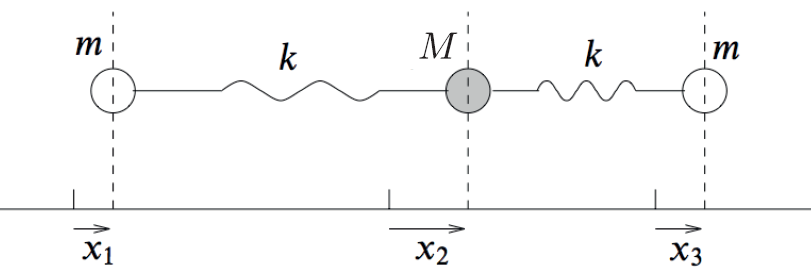
\includegraphics[scale=0.7]{2012P2Q7.PNG}
\end{figure}
where the central atom is carbon which has mass $M$ and the two oxygen atoms have mass $m$. The vibrational motion in the $x$-direction can be modelled by springs joining the carbon atom with the oxygen atoms. Let the springs have spring constant $k$. 
\begin{enumerate}[label=(\roman*)]
\item For vibrations in the $x$-direction, find the normal modes and their eigenfrequencies.\hfill\textbf{[6]}
\item Give a brief explanation for the occurrence of any zero modes.\hfill\textbf{[4]}
\item Suppose that initially the molecule is in equilibrium and the left-hand oxygen atom starts to move with speed $u$ in the positive $x$-direction whilst the other two atoms are stationary. Describe the subsequent motion in terms of the normal modes you have found.\hfill\textbf{[10]}
\end{enumerate}
\end{qns}
\newpage
\begin{ans}\leavevmode
\begin{enumerate}[label=(\roman*)]
\item The potential energy and the kinetic energy are respectively
$$\mathcal{V}=\frac{1}{2}k(x_1-x_2)^2+\frac{1}{2}k(x_2-x_3)^2=\frac{1}{2}\begin{pmatrix}x_1&x_2&x_3\\\end{pmatrix}\begin{pmatrix}k&-k&0\\-k&2k&-k\\0&-k&k\\\end{pmatrix}\begin{pmatrix}x_1\\x_2\\x_3\\\end{pmatrix}:=\frac{1}{2}\mathbf{x}^T\mathbf{V}\mathbf{x}$$
$$\mathcal{T}=\frac{1}{2}m\dot{x}_1^2+\frac{1}{2}M\dot{x}_2^2+\frac{1}{2}m\dot{x}_3^2=\frac{1}{2}\begin{pmatrix}\dot{x}_1&\dot{x}_2&\dot{x}_3\\\end{pmatrix}\begin{pmatrix}m&0&0\\0&M&0\\0&0&m\\\end{pmatrix}\begin{pmatrix}\dot{x}_1\\\dot{x}_2\\\dot{x}_3\\\end{pmatrix}=\frac{1}{2}\mathbf{\dot{x}^TT\dot{x}}$$
Extremize the Lagrangian functional $\mathcal{L}[\mathbf{x},\mathbf{\dot{x}},t]=\mathcal{T}-\mathcal{V}$ and it thus must satisfy the Euler-Lagrange equation $\frac{d}{dt}(\mathbf{T\dot{x}})=-\mathbf{Vx}$. Since $\mathbf{T}$ is not time-dependent, we look for solutions of the form $\mathbf{x}=\mathbf{x_0}e^{i\omega t}$. Solve for $\boldsymbol{0}=(\mathbf{V}-\omega^2\mathbf{T})\mathbf{x_0}$ would be equivalent to solving $$0=\det(\mathbf{V}-\omega^2\mathbf{T})=\det\begin{pmatrix}k-\omega^m&-k&0\\-k&2k-\omega^M&-k\\0&-k&k-\omega^m\\\end{pmatrix}=(k-\omega^2m)(-2km-kM+\omega^2M^2)\omega^2$$
which has solutions $\omega^2=0$, $\omega^2=\frac{k}{m}$ and $\omega^2=\frac{k}{mM}(2m+M)$. Their corresponding eigenvectors are $(1,1,1)^T$, $(1,0,-1)^T$ and $(1,-2\frac{m}{M},1)^T$.
\item By symmetry, the carbon dioxide molecule may translate along the $x$-direction. This translation of its centre of mass corresponds to the zero mode.
\item The general displacement is thus 
$$\mathbf{x}=(c_1+c_2t)\begin{pmatrix}1\\1\\1\\\end{pmatrix}+\text{Re}\bigg[c_3e^{i\sqrt{k/m}t}\bigg]\begin{pmatrix}1\\0\\-1\\\end{pmatrix}+\text{Re}\bigg[c_4e^{i\sqrt{k/Mm}\sqrt{2m+M}t}\bigg]\begin{pmatrix}1\\-2m/M\\1\\\end{pmatrix}$$
where $c_1,c_2\in\mathbb{R}$ and $c_3,c_4\in\mathbb{C}$. The initial conditions are
$$\begin{pmatrix}0\\0\\0\\\end{pmatrix}=\mathbf{x}(t=0)=c_1\begin{pmatrix}1\\1\\1\\\end{pmatrix}+\text{Re}[c_3]\begin{pmatrix}1\\0\\-1\\\end{pmatrix}+\text{Re}[c_4]\begin{pmatrix}1\\-2m/M\\1\\\end{pmatrix}$$
$$\begin{pmatrix}u\\0\\0\\\end{pmatrix}=\mathbf{\dot{x}}(t=0)=c_2\begin{pmatrix}1\\1\\1\\\end{pmatrix}+\text{Re}\bigg[i\sqrt{\frac{k}{m}}c_3\bigg]\begin{pmatrix}1\\0\\-1\\\end{pmatrix}+\text{Re}\bigg[i\sqrt{\frac{k}{Mm}(2m+M)}c_4\bigg]\begin{pmatrix}1\\-2m/M\\1\\\end{pmatrix}$$
Now notice that the eigenvectors are mutually orthogonal with respect to $\mathbf{T}$, i.e.
$$\begin{pmatrix}1&1&1\\\end{pmatrix}\begin{pmatrix}m&0&0\\0&M&0\\0&0&m\\\end{pmatrix}\begin{pmatrix}1\\0\\-1\\\end{pmatrix}=m-m=0$$ $$\begin{pmatrix}1&1&1\\\end{pmatrix}\begin{pmatrix}m&0&0\\0&M&0\\0&0&m\\\end{pmatrix}\begin{pmatrix}1\\-2m/M\\1\\\end{pmatrix}=2m-\frac{2m}{M}M=0$$
$$\begin{pmatrix}1&0&-1\\\end{pmatrix}\begin{pmatrix}m&0&0\\0&M&0\\0&0&m\\\end{pmatrix}\begin{pmatrix}1\\-2m/M\\1\\\end{pmatrix}=m-m=0$$
We exploit this orthogonality to find $c_1,c_2,c_3,c_4$. Denote the inner product with respect to $\mathbf{T}$ to be $\langle.|.\rangle_T$.
$$c_1\langle (1,1,1)^T|(1,1,1)^T\rangle_T=\langle(0,0,0)^T|(1,1,1)^T\rangle_T\implies c_1=0$$
Similarly, $\text{Re}[c_3]=\text{Re}[c_4]=0$. Finally,
$$c_2\langle (1,1,1)^T|(1,1,1)^T\rangle_T=\langle(u,0,0)^T|(1,1,1)^T\rangle_T\implies c_2(2m+M)=mu\implies c_2=\frac{mu}{2m+M}$$
$$-\text{Im}\bigg[\sqrt{\frac{k}{m}}c_3\bigg]\langle (1,0,-1)^T|(1,0,-1)^T\rangle_T=\langle(u,0,0)^T|(1,0,-1)^T\rangle_T\implies -\text{Im}[c_3]2m\sqrt{\frac{k}{m}}=mu$$
$$-\text{Im}\bigg[\sqrt{\frac{k(2m+M)}{mM}}c_4\bigg]\langle (1,-2m/M,1)^T|(1,-2m/M,1)^T\rangle_T=\langle(u,0,0)^T|(1,-2m/M,1)^T\rangle_T$$
which gives $\text{Im}[c_3]=-\frac{u}{2}\sqrt{\frac{k}{m}}$ and $-\sqrt{\frac{k(2m+M)}{mM}}\text{Im}[c_4](2m+\frac{4m^2}{M})=mu\implies \text{Im}[c_4]=\frac{-u}{2+4(m/M)}\sqrt{\frac{mM}{k(2m+M)}}$. Thus, the solution will be
$$\mathbf{x}=\frac{mut}{2m+M}\begin{pmatrix}1\\1\\1\\\end{pmatrix}+\frac{u}{2}\sqrt{\frac{k}{m}}\sin\sqrt{\frac{k}{m}}t\begin{pmatrix}1\\0\\-1\\\end{pmatrix}+\frac{u}{2+4(m/M)}\sqrt{\frac{mM}{k(2m+M)}}\sin\sqrt{\frac{k(2m+M)}{mM}}t\begin{pmatrix}1\\-2m/M\\1\\\end{pmatrix}$$
\end{enumerate}
\end{ans}
\begin{qns}[Group Theory]\leavevmode
\begin{enumerate}[label=(\roman*)]
\item Define the order of a finite group $G$. What is meant by a normal subgroup $H$ of $G$?\hfill\textbf{[2]}
\item Consider $D_4$, the symmetry group of a square. Identify the elements of this group, and explain their geometrical action on the square. List all 8 proper subgroups. Hence identify the order 2 normal subgroup of $D_4$.\hfill\textbf{[8]}
\item Consider now the $D_n$ group, the symmetry group of an $n$-gon for $n > 3$. Prove that when $n$ is even, there exists only one order 2 normal subgroup while when $n$ is odd, there  exists no order 2 normal subgroup.\hfill\textbf{[10]}
\end{enumerate}
\end{qns}
\begin{ans}\leavevmode
\begin{enumerate}[label=(\roman*)]
\item The order of a group $G$ is the number of elements in $G$. A subgroup $H\leq G$ is normal if for every $h\in H$ and $g\in G$, we have $ghg^{-1}\in H$.
\item The symmetry group contains $r$ (rotation by $\pi/2$) and reflection $s$ (about $x$-axis). The commutation relation is $$sr=r^{-1}s\implies r^n=sr^{-n}s\implies sr^p=r^{n-p}s$$
where $n=4$. The group thus contains 
$$\{\Id,r,r^2,r^3,s,sr,sr^2,sr^3\}$$
The proper subgroups are (don't count the group itself and the trivial subgroup): $$\{\Id,r,r^2,r^3\},\quad\{\Id,r^2\},\quad\{\Id,s\},\quad\{\Id,sr\}$$
$$\{\Id,sr^2\},\quad\{\Id,sr^3\},\quad\{\Id,r^2,s,sr^2\},\quad\{\Id,r^2,sr,sr^3\}$$
To have an order 2 normal subgroup, it must contain the identity and one element that squares to the identity. This other element needs to be in a conjugacy class of its own (the identity is also in a conjugacy class of its own). We only have $\{\Id,r^2\}$.
\item The only rotation that commutes with all mirrors is the one for which $p=n-p\implies p=n/2$. When $n$ is even, we only have one order 2 normal subgroup $\{\Id,r^{n/2}\}$, but there is no solution for $n$ odd.. This also follows from Lagrange's theorem, which suggests that $G$ has no order 2 subgroups when $|G|$ is odd.
\end{enumerate}
\end{ans}
\newpage
\begin{qns}[Group Theory]\leavevmode
\begin{enumerate}[label=(\roman*)]
\item Define a homomorphism and an isomorphism between two groups $G_1$ and $G_2$.\hfill\textbf{[2]}\\[5pt]
Let $M(n)$ be the set of all real $n\times n$ matrices.
\item Show that the subset of $M$,
$$GL(n) = \{A \in M \text{  such that }\det(A)\neq 0\}$$
forms a group under the usual law of matrix multiplication.\hfill\textbf{[2]}
\item Show that the following two subsets of $GL(n)$
$$SO(n) = \{A \in M\text{  such that }\det(A) = 1 and AA^T = \text{Id}\}$$
and
$$GL^+(n) = \{A \in M such that \det(A) > 0\}$$
are subgroups of $GL(n)$.\hfill\textbf{[4]}
\item Now consider $SO(2)$, the set of all real $2\times 2$ matrices
$$M=\begin{pmatrix}a&b\\c&d\\\end{pmatrix}$$
such that $MM^T = \Id$ and $\det M = 1$. By finding a suitable parametrization for ($a$, $b$, $c$, $d$), prove that $SO(2)$ is isomorphic to $U(1)$, the group of all complex numbers of modulus one under the usual multiplication of complex numbers.\hfill\textbf{[12]}
\end{enumerate}
\end{qns}
\begin{ans}\leavevmode
\begin{enumerate}[label=(\roman*)]
\item If $G_1$ and $G_2$ are groups, then a function $\phi:~G_1\rightarrow G_2$ is a group homomorphism if $a,b\in G_1$, then
$$\phi(a\cdot_{G_1}b)=\phi(a)\cdot_{G_2}\phi(b)$$
If this homomorphism $\phi$ is invertible, then it is a group isomorphism.
\item Check $\text{GL}(n)$ satsify the group axioms:
\begin{itemize}
\item Closure: Consider $M_1,M_2\in\text{GL}(n)$, then $\det M_1\neq0$, $\det M_2\neq 0$. We must have
$$\det M_1M_2=\det M_1\det M_2\neq 0\implies M_1M_2\in\text{GL}(n)$$
\item Associative: matrix multiplication is associative.
\item Identity: $I_n\in\text{GL}(n)$ since $\det I_n=1\neq 0$.
\item Inverse: $\forall M\in\text{GL}(n)$, then $\det M\neq 0$ and so $M$ is invertible.
\end{itemize}
\item Check the subgroup axioms: for $\text{SO}(n)$,
\begin{itemize}
\item Closure: Consider $A,B\in\text{SO}(n)$, then $\det AB=\det A\det B=1\implies AB\in\text{SO}(n)$.
\item Associative: Inherit from parent group.
\item Identity: $I_n\in\text{SO}(n)$ since $\det I_n=1$.
\item Inverse: $\forall A\in\text{SO}(n)$, $\exists A^{-1}\in\text{SO}(n)$ since $\det A^{-1}=\frac{1}{\det A}=1$.
\end{itemize}
for $\text{GL}^+(n)$:
\begin{itemize}
\item Closure: Consider $A,B\in\text{GL}^+(n)$, then $\det AB=\det A\det B>0\implies AB\in\text{GL}^+(n)$.
\item Associative: Inherit from parent group.
\item Identity: $I_n\in\text{GL}^+(n)$ since $\det I_n=1>0$.
\item Inverse: $\forall A\in\text{GL}^+(n)$, $\exists A^{-1}\in\text{GL}^+(n)$ since $\det A^{-1}=\frac{1}{\det A}>0$.
\end{itemize}
\item We need to construct an isomorphism between $g_p:=e^{i\theta_p}\in\text{U}(1)$ (which is also $\in\mathbb{C}$ with modulus 1) and the matrix
$$A:=\begin{pmatrix}\cos\theta_p&\sin\theta_p\\-\sin\theta_p&\cos\theta_p\\\end{pmatrix}\in\text{SO}(2)$$
since $\det A=\cos^2\theta_p+\sin^2\theta_p=1$. Let this map be $\Phi$. This is a homomorphism.
\begin{align}
    \Phi(g_p)\Phi(g_q)&=\begin{pmatrix}\cos\theta_p&\sin\theta_p\\-\sin\theta_p&\cos\theta_p\\\end{pmatrix}\begin{pmatrix}\cos\theta_q&\sin\theta_q\\-\sin\theta_q&\cos\theta_q\\\end{pmatrix}\nonumber\\&=\begin{pmatrix}\cos\theta_p\cos\theta_q-\sin\theta_p\sin\theta_q&\cos\theta_p\sin\theta_q+\cos\theta_q\sin\theta_p\\-\sin\theta_p\cos\theta_q-\cos\theta_p\sin\theta_q&\cos\theta_p\cos\theta_q-\sin\theta_p\sin\theta_q\\\end{pmatrix}\nonumber\\&=\begin{pmatrix}\cos(\theta_p+\theta_q)&\sin(\theta_p+\theta_q)\\-\sin(\theta_p+\theta_q)&\cos(\theta_p+\theta_q)\\\end{pmatrix}\nonumber\\&=\Phi(g_pg_q)\nonumber
\end{align}
The inverse mapping exists, defined by
$$\Phi^{-1}\bigg(\begin{pmatrix}\cos\theta_p&\sin\theta_p\\-\sin\theta_p&\cos\theta_p\\\end{pmatrix}\bigg)=e^{i\theta_p}$$
and it too is a homomorphism.
\begin{align}
    \Phi^{-1}\bigg(\begin{pmatrix}\cos\theta_p&\sin\theta_p\\-\sin\theta_p&\cos\theta_p\\\end{pmatrix}\bigg)\Phi^{-1}\bigg(\begin{pmatrix}\cos\theta_q&\sin\theta_q\\-\sin\theta_q&\cos\theta_q\\\end{pmatrix}\bigg)&=e^{i(\theta_p+\theta_q)}\nonumber\\&=\Phi^{-1}\bigg(\begin{pmatrix}\cos(\theta_p+\theta_q)&\sin(\theta_p+\theta_q)\\-\sin(\theta_p+\theta_q)&\cos(\theta_p+\theta_q)\\\end{pmatrix}\bigg)\nonumber
\end{align}
Since $\Phi$ is a homomorphism and is bijective, then it is an isomorphism. Hence, $\text{SO}(2)\simeq\text{U}(1)$.
\end{enumerate}
\end{ans}
\newpage
\begin{qns}[Representation Theory]
Any theorems you use should be stated, but need not be proven in this question.
\begin{enumerate}[label=(\roman*)]
\item 
\begin{enumerate}[label=(\alph*)]
\item State the definition of a conjugacy class of a group. State the definition of an
irreducible representation.\hfill\textbf{[1]}\\[5pt]
Consider the quaternion group $\mathcal{Q} = \{\pm 1,\pm i,\pm j,\pm k\}$ with the defining relations
$$−1 = i^2 = j^2 = k^2 = ijk$$
\item Find all conjugacy classes of $\mathcal{Q}$. Hence deduce the number of irreducible representations of $\mathcal{Q}$ and state their dimensions.\hfill\textbf{[8]}
\end{enumerate}
\item 
\begin{enumerate}[label=(\alph*)]
\item Consider the 3-dimensional real matrix representation $T$ of the order 4 cyclic
group $Z_4 = \{I, a, a^2, a^3\}$ given by
$$T(a)=\begin{pmatrix}1&0&0\\0&0&b\\0&c&0\\\end{pmatrix}$$
What are the conditions on the real constants $b$ and $c$ such that $T$ is (i) a faithful representation, and (ii) an unfaithful representation?\hfill\textbf{[7]}
\item
Finally, construct a 2-dimensional representation of $Z_4$ with kernel $\{I, a^2\}$.\hfill\textbf{[3]}
\end{enumerate}
\end{enumerate}
\end{qns}
\begin{ans}\leavevmode
\begin{enumerate}[label=(\roman*)]
\item
\begin{enumerate}[label=(\alph*)]
\item The conjugacy class of $h\in G$ is the set of possible outputs to the process $gg_ig^{-1}$ by systematically conjugating $h$ with each element of $G$ in turn (written as $\ccl(h)$), and is
$$\ccl(h):=\{k\in G\text{ s.t. }k=g\cdot h\cdot g^{-1}\text{ for some }g\in G\}$$
A representation $D$ of a group $G$ is a homomorphic mapping from the group elements to the set of invertible matrices, i.e. $D(g_i)$ is an invertible matrix for $g_i\in G$. A representation is said to be reducible if $\exists$ an invertible matrix $S$ s.t. $SD(g_i)S^{-1}$ has the same block-diagonal form (the entire space being the invariant subspace does not count) $\forall M(g_i)$. If no such matrix can be found, then the representation is said to be irreducible.
\item $\pm1$ are respectively in their conjugate classes of their own. Other conjugacy classes are
$$\{i,-i\},\quad\{j,-j\},\quad\{k,-k\}$$
Since the number of irreducible representations is the number of conjugacy classes, there are thus 5 irreducible representations. Furthermore, since the sum of the squares of the dimensions of the matrices of the distinct irreducible representations is the order of the group, we require 5 positive integers whose squares sum to 8. They must be
$$\{2,1,1,1,1\}$$
\end{enumerate}
\item 
\begin{enumerate}[label=(\alph*)]
\item Since $T$ is a representation, it must be a homomorphic mapping. We have
$$T(a)=\begin{pmatrix}1&0&0\\0&0&b\\0&c&0\\\end{pmatrix},~ T(a)^2=\begin{pmatrix}1&0&0\\0&bc&0\\0&0&bc\\\end{pmatrix},~ T(a)^3=\begin{pmatrix}1&0&0\\0&0&b^2c\\0&bc^2&0\\\end{pmatrix},~ T(a)^4=\begin{pmatrix}1&0&0\\0&b^2c^2&0\\0&0&b^2c^2\\\end{pmatrix}$$
We require $T(I)=T(a^4)=T(a)^4$, so $b^2c^2=1$. We either have $bc=-1$ (then $T(a)$, $T(a)^2=T(a^2)$, $T(a)^3=T(a^3)$ and $T(a)^4=T(a^4)$ are distinct matrices, hence faithful representation) or $bc=+1$ (unfaithful representation with kernel $\{I,a^2\}$ since $T(a^2)=T(a)^2=I$).
\item The two-dimensional representation with kernel $\{I,a^2\}$ is the two-dimensional sub-block in the unfaithful representation $T$. Since $bc=1$, we choose $b=c=1$ for convenience. Then, let this representation be $U$
$$U(a)=\begin{pmatrix}0&1\\1&0\\\end{pmatrix}=U(a^3),\quad U(a^2)=\begin{pmatrix}1&0\\0&1\\\end{pmatrix}=U(a^4)$$
\end{enumerate}
\end{enumerate}
\end{ans}
\newpage
\section{2013}
\subsection{Paper 1}
\begin{qns}[Vector Calculus]\leavevmode
\begin{enumerate}[label=(\roman*)]
    \item Using Cartesian coordinates, show that for arbitrary vector fields $\mathbf{A}(x,y,z)$ and $\mathbf{B}(x,y,z)$\hfill \textbf{[6]}
$$\boldsymbol{\nabla}\cdot(\mathbf{A}\times\mathbf{B})=\mathbf{B}\cdot(\boldsymbol{\nabla}\times\mathbf{A})-\mathbf{A}\cdot(\boldsymbol{\nabla}\times\mathbf{B})$$
\item State the divergence theorem, and use it to show that for a scalar field $a(x,y,z)$ and a vector field $\mathbf{B}(x,y,z)$,
\begin{equation}
  \int_V\boldsymbol{\nabla}a\cdot(\boldsymbol{\nabla}\times\mathbf{B})dV=-\int_S(\boldsymbol{\nabla}a\times\mathbf{B})\cdot\mathbf{\hat{n}}dS\tag{*}  
\end{equation}
where $V$ is a given volume, and $\mathbf{\hat{n}}$ is the unit vector outward normal to its surface $S$.\hfill \textbf{[6]}
\item  Consider the particular case $a=xy+z^2$ and $\mathbf{B}=(y,-yz,x)$.\\[5pt]
Verify both sides of (*), where $V$ is a circular cylinder of height $h$ and radius 1 with base $x^2+y^2=1$ at $z=0$.\hfill \textbf{[8]}
\end{enumerate}
\end{qns}
\begin{ans}\leavevmode
\begin{enumerate}[label=(\roman*)]
    \item Using suffix notation in Cartesian coordinates, then evaluating the LHS:
$$\frac{\partial}{\partial x_k}\epsilon_{ijk}A_iB_j=\epsilon_{ijk}B_j\frac{\partial}{\partial x_k}A_i+\epsilon_{ijk}A_i\frac{\partial B_j}{\partial x_k}=B_j\epsilon_{kij}\frac{\partial A_i}{\partial x_k}-A_i\epsilon_{kji}\frac{\partial B_j}{\partial x_k}$$
 where $\epsilon_{jki}=-\epsilon_{kji}$.
\item If $\mathbf{F}=\mathbf{F}(\mathbf{x})$ be a continuously differentiable vector field and $D\subset\mathbb{R}^2$ a region with piecewise smooth boundary $\partial D$, then the divergence theorem states
$$ \int_D\boldsymbol{\nabla}\cdot\mathbf{F}dA=\oint_{\partial D}\mathbf{F}\cdot d\mathbf{n}ds$$
where the normal to $\partial V$ points outwards from $V$. Invoke divergence theorem to part (i)'s result, and let $\mathbf{A}=\boldsymbol{\nabla}a$, $V=D$, $\partial V=S$,
$$\int_S(\boldsymbol{\nabla}a\times\mathbf{B})\cdot\mathbf{\hat{n}}dS=\int_V\boldsymbol{\nabla}\cdot(\boldsymbol{\nabla}a\times\mathbf{B})dV=\int_V\mathbf{B}\cdot(\boldsymbol{\nabla}\times\boldsymbol{\nabla}a)-\boldsymbol{\nabla}a\cdot(\boldsymbol{\nabla}\times\mathbf{B})dV$$
Since the curl of a gradient is zero, the result trivially follows.
\item We have $\boldsymbol{\nabla}a=(y,x,2z)^T$ and $\boldsymbol{\nabla}\times\mathbf{B}=(y,-1,-1)^T$. So, $\boldsymbol{\nabla}a\cdot(\boldsymbol{\nabla}\times\mathbf{B})=y^2-x-2z$ and $\boldsymbol{\nabla}a\times\mathbf{B}=(x^2+2yz^2,2zy-xy,-y^2z-xy)^T$. We parametrize $S=S_1\cup S_2\cup S_3$ with $S_1:$ $z=0$ and $\mathbf{\hat{n}}=-\mathbf{\hat{z}}$; $S_2:$ $z=h$ and $\mathbf{\hat{n}}=\mathbf{\hat{z}}$; $S_3:$ $\mathbf{\hat{n}}=\mathbf{\hat{r}}$. We note for all 3 surfaces, $x^2+y^2=1$. Then, the surface integral gives
\begin{eqnarray}
&&\int_{S_1}xydxdy+\int_{S_2}-y^2h-xydxdy+\int_0^h\int_0^{2\pi}\begin{pmatrix}\cos^2\theta+2\sin\theta z^2\\2z\sin\theta-\sin\theta\cos\theta\\-\sin^2\theta z-\cos\theta\sin\theta\\\end{pmatrix}\cdot\begin{pmatrix}\cos\theta\\\sin\theta\\0\\\end{pmatrix}d\theta dz\nonumber\\&=&-\frac{h}{4}\int_0^{2\pi}\sin^2\theta d\theta+\int_0^{2\pi}h\cos^3\theta+\frac{2}{3}h^3\sin\theta\cos\theta+h^2\sin^2\theta-h\sin^2\theta\cos\theta d\theta\nonumber\\&=&-\frac{h}{4}\int_0^{2\pi}\sin^2\theta d\theta+\int_0^{2\pi}h\cos\theta\cos2\theta d\theta+h^2\int_0^{2\pi}\frac{2}{3}h\sin\theta\cos\theta+\sin^2\theta d\theta\nonumber\\&=& \bigg(h^2-\frac{h}{4}\bigg)\pi\nonumber
\end{eqnarray}
where we cancel the first term with part of the second term, since the two regions have the same integration limits for $x,y$. We also used $\int_0^{2\pi}\sin\theta\cos\theta d\theta=0$, $\int_0^{2\pi}\cos2\theta\cos\theta d\theta=0$ and $\int_0^{2\pi}\sin^2\theta d\theta=\pi$. This is indeed the negative of the volume integral:
$$\int_0^h\int_0^1\int_0^{2\pi}r^3\sin^2\theta-r^2\cos\theta-2rzd\theta drdz=\frac{1}{4}\pi h-\pi h^2$$
Hence, the identity in part (ii) was verified.
\end{enumerate}
\end{ans}
\newpage
\begin{qns}[Partial Differential Equation]
A damped wave on a string can be described by the equation
$$\frac{\partial^2u}{\partial t^2}=c^2\frac{\partial^2u}{\partial x^2}-\alpha\frac{\partial u}{\partial t}$$
where subscripts denote partial derivatives and $\alpha$ and $c$ are constants.
\begin{enumerate}[label=(\roman*)]
    \item Use the method of separation of variables to find two ordinary differential equations.\hfill \textbf{[4]}
    \item Consider a string between $-L\leq x\leq L$ with fixed endpoints $u(x=-L)=u(x=L)=0$. If the string is plucked in the centre, we might expect the solutions to be symmetric about $x=0$. Show that the general solution for symmetric disturbances to be written in the following form
\begin{equation}
u(x,t)=\sum_{n=1}^\infty e^{-\alpha t/2}\cos\bigg(\frac{n\pi x}{2L}\bigg)\text{Re}[A_ne^{i\omega_nt}+B_ne^{-i\omega_nt}]\tag{*}
\end{equation}
where $n$ is an odd integer and $\text{Re}$ denotes real part.\hfill \textbf{[6]}
\item Give an expression for $\omega_n$ as a function of $\alpha$, $n$, $L$ and $c$. How small must the damping coefficient, $\alpha$, be for oscillatory solutions to exist? Describe what happens if $\alpha<0$.\hfill \textbf{[3]}
\item If the string is plucked so that at $t=0$,
$$\frac{\partial u}{\partial t}=0,\quad u(x,t=0)=e^{-|x|/l}$$
find the coefficients $A_n$ and $B_n$ in (*). How do the coefficients simplify in the limit when $l<<L$, as required to impose $u(x=-L)=u(x=L)=0$. \hfill \textbf{[7]}
\end{enumerate}
\end{qns}
\begin{ans}\leavevmode
\begin{enumerate}[label=(\roman*)]
    \item Use separation of variables $u(x,t)=X(x)T(t)$ such that
$$\frac{T''(t)}{T(t)}=c^2\frac{X''(x)}{X(x)}-\alpha\frac{T'(t)}{T(t)}=-\lambda^2$$
to obtain two ordinary differential equations
\begin{equation}
\frac{d^2T(t)}{dt^2}+\alpha \frac{dT(t)}{dt}+\lambda^2T(t)=0\tag{time}
\end{equation}
\begin{equation}
    \frac{d^2X(x)}{dx^2}=-\frac{\lambda^2}{c^2}X(x)\tag{position}
\end{equation}
\item The corresponding solutions are
$$X(x)=c_1\sin\frac{\lambda}{c}x+c_2\cos\frac{\lambda}{c}x$$
$$T(t)=e^{-\alpha t/2}(c_3e^{0.5\sqrt{\alpha^2-4\lambda^2}t}+c_4e^{-0.5\sqrt{\alpha^2-4\lambda^2}t})$$
Since $u(x=-L)=u(x=L)=0$, only the term $\cos\frac{n\pi x}{2L}$ for odd $n$ matters (since symmetric about $x=0$) for $X(x)$. We have $\lambda=\frac{nc\pi}{2L}$ and $\omega_n=0.5\sqrt{4\lambda^2-\alpha^2}=\sqrt{\frac{c^2n^2\pi^2}{4L^2}-\frac{\alpha^2}{4}}$. Hence, we obtain the desired form for $u(x,t)$.
$$u(x,t)=\sum_{n=1}^\infty X_n(x)T_n(t)=\sum_{n=1}^\infty e^{-\alpha t/2}\cos\bigg(\frac{n\pi x}{2L}\bigg)\text{Re}[A_ne^{i\omega_nt}+B_ne^{-i\omega_nt}]$$
\item Since $n$ can be arbitrarily high, oscillatory solutions will always exist. For $\alpha<0$, the system is unstable.
\item The time derivative at for $u$ at $t=0$ is
$$0=\frac{\partial u(x,t)}{\partial t}\bigg|_{t=0}=\sum_{n=1}^\infty\cos\frac{n\pi x}{2L}\bigg(\omega_n\text{Im}[B_n-A_n]-\frac{\alpha}{2}\text{Re}[A_n+B_n]\bigg)\implies\text{Im}[B_n-A_n]=\frac{\alpha}{2\omega_n}\text{Re}[A_n+B_n]$$
We have $e^{-|x|/l}=u(x,0)=\sum_{n=1}^\infty\cos(\frac{n\pi x}{2L})\text{Re}[A_n+B_n]$ and so
\begin{eqnarray}
\int_{-L}^Le^{-|x|/l}\text{Re}[e^{im\pi x/2L}]dx&=&\sum_{n=1}^\infty\text{Re}[A_n+B_n]\int_{-L}^L\cos\frac{m\pi x}{2L}\cos\frac{n\pi x}{2L}dx\nonumber\\2\int_{0}^Le^{-l^{-1}(1-\frac{im\pi l}{2L}x)dx}&=&\sum_{n=1}^\infty\text{Re}[A_n+B_n]\delta_{nm}L\nonumber\\2\text{Re}\bigg[\frac{-l}{1-\frac{im\pi l}{2L}}\bigg(e^{-Ll^{-1}(1-\frac{im\pi l}{2L})}-1\bigg)\bigg]&=&L\text{Re}[A_m+B_m]\nonumber
\end{eqnarray}
To write $u(x,t)$ in terms of $\cos(\omega_nt)$ and $\sin(\omega_nt)$, we require $A_n=B_n^*$. This means $$B_n=\frac{1}{L}\text{Re}\bigg[\frac{-l}{1-\frac{in\pi l}{2L}}\bigg(e^{-Ll^{-1}(1-\frac{in\pi l}{2L})}-1\bigg)\bigg]\bigg(1+i\frac{\alpha}{2\omega_n}\bigg)$$
$$A_n=\frac{1}{L}\text{Re}\bigg[\frac{-l}{1-\frac{in\pi l}{2L}}\bigg(e^{-Ll^{-1}(1-\frac{in\pi l}{2L})}-1\bigg)\bigg]\bigg(1-i\frac{\alpha}{2\omega_n}\bigg)$$
Further, we note that due to symmetry we have to take odd $n$ only such that $e^{in\pi/2}=i(-1)^n$. In the limit $l<<L$, we have
$$A_n\approx\frac{l}{L}\text{Re}\bigg[l\bigg(1+\frac{in\pi l}{2L}\bigg)\bigg]\bigg(1-i\frac{\alpha}{2\omega_n}\bigg)=\frac{l}{L}\bigg(1-i\frac{\alpha}{2\omega_n}\bigg)$$
$$B_n\approx\frac{1}{L}\text{Re}\bigg[l\bigg(1+\frac{in\pi l}{2L}\bigg)\bigg]\bigg(1+i\frac{\alpha}{2\omega_n}\bigg)=\frac{l}{L}\bigg(1+i\frac{\alpha}{2\omega_n}\bigg)$$
\end{enumerate}
\end{ans}
\newpage
\begin{qns}[Green's Functions]\leavevmode
\begin{enumerate}[label=(\roman*)]
\item Find the general solution $y(x)$ to the homogeneous second-order linear differential equation

\hfill \textbf{[6]}
$$\frac{d^2y}{dx^2}-\frac{1+x}{x}\frac{dy}{dx}+\frac{y}{x}=0$$
[Hint: Look for a particular solution of the form $y_p(x)=g(x)e^x$.]
\item Find the Green's function for this equation in the region $-1\leq x\leq 1$, subject to the homogeneous boundary conditions $y(-1)=0$ and $y(1)=0$.\hfill \textbf{[8]}
\item Use the Green's function found above to solve the inhomogeneous differential equation
$$\frac{d^2y}{dx^2}-\frac{1+x}{x}\frac{dy}{dx}+\frac{y}{x}=x$$
subject to the same boundary conditions. \hfill \textbf{[6]}
\end{enumerate}
\end{qns}
\begin{ans}\leavevmode
\begin{enumerate}[label=(\roman*)]
\item We try their suggested form of $y_p$. We then have
$$\bigg(g''+2g'+g-\frac{1}{x}g'-\frac{1}{x}g-g'-g+\frac{1}{x}g\bigg)e^x=0\implies g''=g'\frac{1-x}{x}$$
This means the solution is $\frac{dg}{dx}=e^{\ln(x)-x+C}=Axe^{-x}\implies g(x)=-Ae^{-x}(1+x)+B\implies y(x)=-A(1+x)+Be^x$.
\item The corresponding Green's function satisfy 
$$\frac{\partial^2G(x,\xi)}{\partial x^2}-\frac{1+x}{x}\frac{\partial G(x,\xi)}{\partial x}+\frac{G(x,\xi)}{x}=\delta(x-\xi),\quad -1\leq x\leq 1,\quad G(-1,\xi)=0=G(1,\xi)$$
Integrate this over an infinitesimal region about $x=\xi$, we deduce that $G'$ satisfy the jump condition $[G']_{\xi^-}^{\xi^+}=1$ at $x=\xi$ and $G$ to be continuous everywhere (otherwise $G''\propto\delta'(x-\xi)$ which is a contradiction), including $x=\xi$. Using the homogeneous solution in part (i), our Green's function will have the form
$$G(x,\xi)=
\left\{
        \begin{array}{ll}
      A(\xi)(1+x)& -1\leq x<\xi\leq1 \\
      C(\xi)[(1+x)-2e^{x-1}]& -1\leq\xi<x\leq 1
        \end{array}
    \right.$$
We have $\frac{\partial G}{\partial x}=A$ for $-1\leq x<\xi<1$ and $C(\xi)[1-2e^{x-1}]$ for $-1\leq\xi<x\leq1$. Jump condition and continuity condition respectively give $$C(\xi)[1-2e^{x-1}]-A(\xi)=1$$ $$A(\xi)(1+\xi)=C(\xi)((1+\xi)-2e^{\xi-1})$$
We thus have $C(\xi)=-(\frac{1+\xi}{2\xi})e^{1-\xi}$ and $A(\xi)=-\frac{1}{2\xi}[(1+\xi)e^{1-\xi}-2]$. The Green's function is
$$G(x,\xi)=
\left\{
        \begin{array}{ll}
      \frac{1}{2\xi}(1+x)[2-(1+\xi)e^{1-\xi}]& -1\leq x<\xi\leq1 \\
      \frac{1}{2\xi}(1+\xi)e^{-\xi}[2e^x-(1+x)e] & -1\leq\xi<x\leq 1
        \end{array}
    \right.$$
\item The solution is $y=\int_{-1}^1G(x,\xi)f(\xi)d\xi$, where $f(x)=x$.
$$y=[2e^x-(1+x)e]\int_{-1}^x\frac{1}{2\xi}(1+\xi)e^{-\xi}\xi d\xi+(1+x)\int_x^1\frac{1}{2\xi}[2-(1+\xi)e^{1-\xi}]\xi d\xi$$
Since $\int(1+\xi)e^{-\xi}d\xi=-(2+\xi)e^{-\xi}$, we have
$$y(x)=\frac{1}{2}[2e^{x+1}-2x^2+(1+e^2)(x+1)]$$
\end{enumerate}
\end{ans}
\newpage
\begin{qns}[Fourier Transform]
The Fourier transform $\tilde{f}(k)$ of a function $f(x)$ is defined by
$$\tilde{f}(k)=\int_{-\infty}^\infty e^{-ikx}f(x)dx$$
and the correlation $h(x)$ between two functions $f(x)$ and $g(x)$ is defined by
$$h(x)=\int_{-\infty}^\infty(f(y))^*g(x+y)dy$$
where $*$ denotes a complex conjugate.
\begin{enumerate}[label=(\roman*)]
\item Prove that \hfill \textbf{[6]} $$\tilde{h}(k)=(\tilde{f}(k))^*\tilde{g}(k)$$
\item Use this result to prove Parseval's Theorem \hfill \textbf{[6]}
$$\int_{-\infty}^\infty|f(x)|^2dx=\frac{1}{2\pi}\int_{-\infty}^\infty|\tilde{f}(k)|^2dk$$
\item Verify Parseval's theorem for the following function\hfill \textbf{[8]}
$$f(x)=
\left\{
        \begin{array}{ll}
      1 & |x|\leq 1 \\
      0 & |x|>1
        \end{array}
    \right.$$
\end{enumerate}
\begin{mdframed}
\textcolor{darkblue}{Hint: $\int_0^\infty x^{-1}\sin(x)\cos(x)dx=\frac{\pi}{4}$}
\end{mdframed}
\end{qns}
\begin{ans}\leavevmode
\begin{enumerate}[label=(\roman*)]
\item The standard proof for convolution theorem: set $x=u-y$ and separate the integrals.
$$\tilde{h}(k)=\int_{-\infty}^\infty\int_{-\infty}^\infty f^*(y)g(x+y)dye^{-ikx}dx=\int_{-\infty}^\infty f^*(y)e^{iky}dy\int_{-\infty}^\infty g(u)e^{-iku}du=(\tilde{f}(k))^*\tilde{g}(k)$$
\item Another standard proof. From the previous result, set $f=g$, and integrate over $k$
$$\int_{-\infty}^\infty\tilde{h}(k)dk=\int_{-\infty}^\infty\int_{-\infty}^\infty\int_{-\infty}^\infty f^*(y)f(x+y)e^{-ikx}dydxdk$$
Rearranging, we have
\begin{eqnarray}
\int_{-\infty}^\infty|\tilde{f}(k)|^2dk&=&\int_{-\infty}^\infty f^*(y)\int_{-\infty}^\infty f(x+y)\int_{-\infty}^\infty e^{-ikx}dkdxdy\nonumber\\&=&\int_{-\infty}^\infty f^*(y)\int_{-\infty}^\infty f(x+y)2\pi\delta(x)dxdy\nonumber\\&=&2\pi\int_{-\infty}^\infty|f(y)|^2dy\nonumber
\end{eqnarray}
\item The norm is trivially $\int_{-\infty}^\infty|f(x)|^2dx=\int_{-1}^1dx=2$. Also, the Fourier transform is $\tilde{f}(k)=\int_{-1}^1e^{-ikx}dx=\frac{2\sin(k)}{k}$. We then have
$$\frac{1}{2\pi}\int_{-\infty}^\infty|\tilde{f}(k)|^2dk=\frac{4}{2\pi}2\int_0^\infty\frac{\sin^2k}{k^2}dk=\frac{4}{\pi}\bigg([-k^{-1}\sin^2k]^\infty_0+\int_0^\infty\frac{2\sin(k)\cos(k)}{k}dk\bigg)=\frac{4}{\pi}2\frac{\pi}{4}=2$$
which is consistent with Parseval's theorem.
\end{enumerate}
\end{ans}
\newpage
\begin{qns}[Linear Algebra]\leavevmode
\begin{enumerate}[label=(\roman*)]
\item If $M$ is an invertible complex matrix with Hermitian conjugate $M^\dag$ and inverse $M^{−1}$, show that \hfill \textbf{[2]}
$$(M^\dag)^{−1} = (M^{−1})^\dag$$
\item If $A$ is an anti-Hermitian matrix, i.e. one such that $A^\dag=-A$, show, by diagonalizing $iA$, that
$$|\det(1 + A)|^2\geq1$$
and hence that $1 + A$ is always invertible.\hfill \textbf{[6]}
\item If $A$ is an anti-Hermitian matrix, show that
\begin{equation}
    U = (1 − A)(1 + A)^{-1}\tag{*}
\end{equation}
is a unitary matrix, that is $U^\dag = U^{−1}$.\hfill \textbf{[6]}
\item If $U$ is a unitary matrix such that $1 + U$ is invertible, show that there is a unique matrix $A$ satisfying (*). Show that the matrix $A$ is indeed anti-Hermitian. Give an example of a unitary matrix for which $1 + U$ is not invertible. \hfill \textbf{[6]}
\end{enumerate}
\end{qns}
\begin{ans}\leavevmode
\begin{enumerate}[label=(\roman*)]
\item Take conjugate transpose of $MM^{-1}=I$ gives $(M^{-1})^\dag M^\dag=I\implies (M^{-1})^\dag=(M^\dag)^{-1}$.
\item If $A$ is anti-Hermitian, then $iA$ is Hermitian, i.e. $A^\dag=-A\implies(iA)^\dag=-iA^\dag=iA$. To show $iA$ is diagonalizable, it must have $n$ linearly independent eigenvectors. Being Hermitian, its eigenvalues are real and the eigenvectors corresponding to different eigenvalues are orthogonal: 
$$(iA)x_q=\lambda_qx_q\implies x_p^\dag(iA)x_q=\lambda_qx_p^\dag x_q\implies(\lambda_p x_p)^\dag x_q=\lambda_qx_p^\dag x_q\implies(\lambda_p^*-\lambda_q)x_p^\dag x_q=0$$
$x_p^\dag x_q=1$ iff $p=q$, then $\lambda_p^*=\lambda_p\in\mathbb{R}$ $\forall p$. $x_p^\dag x_q=0$ iff $\lambda_p^*-\lambda_q\neq0$. If $iA$ has $n$ distinct eigenvalues, we get a basis of $n$ pairwise orthogonal vectors. Otherwise, say we have $r<n$ distinct eigenvalues, then by Gram-Schmidt, we can extend the $r$ orthogonal eigenvectors into a basis for $\mathbb{C}^n$. Thus, $iA$ is guaranteed to have $n$ linearly independent eigenvectors.\\[5pt]
Having established that $iA$ is diagonalizable, one can construct a matrix $R$ whose columns are the normalized eigenvectors of $iA$ such that $R^\dag iAR$ is diagonal with real eigenvalues. Then,
$$\det(I+A)=\det((RR^\dag)(I+A))=\det(R^\dag(I+A)R)=\det(I+\Lambda)=\prod_{i=1}^n(1+\lambda_i)$$
where $\Lambda=\diag(\lambda_1,...,\lambda_n)$ and $\lambda_i$ is imaginary, since $A$ is anti-Hermitian. Hence
$$|\det(1+A)|^2=\prod_{i=1}^n(1+\lambda_i)(1+\lambda_i^*)=1+|\lambda_i|^2\geq1$$
Since the $\det\neq0$, $1+A$ is always invertible.
\item We have $A^\dag=-A$ and from part (ii), $1+A$ is invertible so by part (i), $((1+A)^{-1})^\dag=((1+A)^\dag)^{-1}=(1-A)^{-1}$.
$$U^\dag=[(1-A)(1+A)^{-1}]^\dag=[(1+A)^{-1}]^\dag(1-A)^\dag=(1-A)^{-1}(1+A)$$
To show $U$ is unitary, we need to further show that $1+A$ and $1-A$ commute, i.e.
$$[1+A,1-A]=(1+A)(1-A)-(1-A)(1+A)=1-A+A-A^2-1-A+A-A^2=0$$
$$\implies U^\dag U=(1-A)^{-1}(1+A)(1-A)(1+A)^{-1}=(1-A)^{-1}(1-A)(1+A)(1+A)^{-1}=I$$
so $U$ is unitary, i.e. $U^\dag=U^{-1}$.
\item Since $U=(1-A)(1+A)^{-1}$, we naturally have $U(1+A)=1-A$. Taking conjugate transpose on both sides, $(1+A)^\dag U^\dag=(1-A)^\dag=(1-A^\dag)$ and hence
$$(1-A^\dag)(1-A)=(1+A^\dag)U^\dag U(1+A)=(1+A^\dag)(1+A)\implies A^\dag=-A$$
where we used the fact that $U$ is unitary to show $A$ is anti-Hermitian.\\[5pt]
One example of $1+U$ being non-invertible is $U=-I$.
\end{enumerate}
\end{ans}
\newpage
\begin{qns}[Linear Algebra]\leavevmode
\begin{enumerate}[label=(\roman*)]
\item If $M$ is an anti-symmetric $n\times n$ matrix show that
$$\det(M) = (−1)^{n}\det(M)$$
and hence if $n$ is odd, $\det(M)$ must vanish. \hfill \textbf{[2]}
\item If $M$ is a real anti-symmetric $n\times n$ matrix show that $M^2$ is a real symmetric non-positive matrix, i.e. $$x^TM^2x\leq0$$
for all vectors x, where $^T$ denotes transpose. Hence show that if $n$ is odd then $M^2$ must have at least one vanishing eigenvalue.\hfill \textbf{[3]}
\item If $e_1$ is an eigenvector of $M^2$ with non-vanishing eigenvalue $\lambda_1=-\mu_1^2$, with $\mu_1>0$,
show that $e_2 = Me_1$ is also an eigenvector of $M^2$, orthogonal to $e_1$ with the same eigenvalue.\hfill \textbf{[5]}
\item By considering the remaining eigenvectors, $\{e_3,...,e_n\}$, conclude that the non-vanishing eigenvalues of $M^2$ occur in, not necessarily distinct, pairs.\hfill \textbf{[4]}
\item Hence show, using the basis of eigenvectors of $M^2$ , that the original matrix $M$ may be cast in block diagonal form with each block being either $2\times 2$ anti-symmetric with entries $\pm\mu_1$, $\pm\mu_2$, $\dots$ or a block with zero entries.\hfill \textbf{[6]}
\end{enumerate}
\end{qns}
\begin{ans}\leavevmode
\begin{enumerate}[label=(\roman*)]
\item If $M$ is anti-symmetric, $M^T=-M$, then $\det M=\det(M^T)=\det(-M)=(-1)^n\det(M)$. For odd $n$, $\det(M)=-\det(M)\implies\det(M)=0$.
\item Consider $y=Mx$. We have $|y|^2\geq0$ $\forall x$. So
$$0\leq|y|^2=(Mx)^TMx=x^TM^TMx=-x^TMMx\implies x^TM^2x\leq0$$
If $n$ is odd, $\det M=0$ from earlier, then at least one of the eigenvalues of $M$ is 0, since $\det M=\prod_{i=1}^n\lambda_i=0$. Then, $0x=Mx=M^2x$, $M^2$ has at least one vanishing eigenvalue.
\item Given $M^2e_1=-\mu_1^2e_1$, $M^2e_2=M^2Me_1=MM^2e_1=-\mu_1^2Me_1=-\mu_1^2e_2$, and so $e_2$ is an eigenvector of $M^2$ with eigenvalue $-\mu_1^2$ as well.\\[5pt]
Consider $e_1\cdot e_2=(e_1\cdot e_2)^T$, which is a scalar.
$$0=e_1\cdot e_2-(e_1\cdot e_2)^T=e_1^TMe_1-e_2^Te_1=e_1^TMe_1-e_1^TM^Te_1=e_1^TMe_1+e_1^TMe_1$$
where $M$ is anti-symmetric. So, $0=e_1^TMe_1=e_1\cdot e_2$, i.e. $e_1$ and $e_2$ are orthogonal.
\item From part (iii), each eigenvector corresponding to a non-zero eigenvalue will generate a 2D subspace under the action of arbitrary powers of $M$, each vector within each subspace having the same eigenvalue.\\[5pt]
Eigenvalues may be repeated within different subspaces. 2D subspaces with different eigenvalues are disjoint, whilst those subspaces with repeated eigenvalues can be chosen to be disjoint.
\item Assume $\hat{e}_1$ is an eigenvector of $M^2$ with eigenvalue of $\lambda=-\mu_1^2$, then $e_2=M\hat{e}_1$ will not, in general, be properly normalized.
$$e_2\cdot e_2=(M\hat{e}_1)^TM\hat{e_1}=-\hat{e}_1^TM^2\hat{e}_1=\mu_1^2$$
since $M$ is anti-symmetric. So, we can construct the normalized version $\hat{e}_2=\frac{1}{\mu_1}M\hat{e}_1$. Then, $\hat{e}_1^TM\hat{e}_2=\hat{e}_1^T\frac{1}{\mu_1}M^2\hat{e}_1=\mu_1$. Consider orthogonal matrix $R$, whose columns are the normalized eigenvectors of $M^2$, then $R^TMR$ has diagonal entries to be zero. In particular, the absolute values of (1,2) and (2,1) entries are $\mu_1$ and $-\mu_1$ respectively such that $M$ is anti-symmetric..
\end{enumerate}
\end{ans}
\newpage
\begin{qns}[Cauchy-Riemann]\leavevmode
\begin{enumerate}[label=(\roman*)]
\item Write down the Cauchy Riemann equations for the real and imaginary parts, $u$, $v$ of the analytic function $f(z) = u(x, y)+iv(x, y)$, where $z = x+iy$ and hence show that the level sets, $u =$ constant and $v =$ constant, are orthogonal, and that $|\nabla u| = |\nabla v|$.\hfill \textbf{[3]}
\item Show that $u$ satisfies Laplace’s equation $\nabla^2 u=(\partial_x^2+\partial_y^2)u$, where $\partial_x=\frac{\partial}{\partial x}$, $\partial_y=\frac{\partial}{\partial y}$.\hfill \textbf{[2]}
\item Using the analytic function $f(z) = \cosh^{−1} z$, show that the level sets $u =$ constant and $v =$ constant form an orthogonal system of ellipses and hyperbolae.\hfill \textbf{[5]}
\item Hence show that $\phi=u-\cosh^{-1}(\sqrt{2})$ is a solution of Laplace’s equation which vanishes on the ellipse
$$\frac{1}{2}x^2+y^2=1$$
How does $\phi$ behave as $x,y\rightarrow\infty$?\hfill \textbf{[5]}
\item If $$F(z,\overline{z})=\overline{z}H(z)+G(z)=U(x,y)+iV(x,y)$$
where $H(z)$ and $G(z)$ are analytic functions of $z$ and $\overline{z}=x-iy$, show that $U$ and $V$ satisfy the fourth order partial differential equations \hfill \textbf{[5]}
$$\nabla^4U=(\partial_x^2+\partial_y^2)(\partial_x^2+\partial_y^2)U=0$$
$$\nabla^4V=(\partial_x^2+\partial_y^2)(\partial_x^2+\partial_y^2)V=0$$
\end{enumerate}
\end{qns}
\begin{ans}\leavevmode
\begin{enumerate}[label=(\roman*)]
\item For $f(z)=u(x,y)+iv(x,y)$ to be analytic, $f(z)$ must satisfy the Cauchy-Riemann equations $\frac{\partial u}{\partial x}=\frac{\partial v}{\partial y}$ and $\frac{\partial u}{\partial y}=-\frac{\partial v}{\partial x}$. Then, we use them to evaluate
$$\boldsymbol{\nabla}u\cdot\boldsymbol{\nabla}v=\frac{\partial u}{\partial x}\frac{\partial v}{\partial x}+\frac{\partial u}{\partial y}\frac{\partial v}{\partial y}=\frac{\partial v}{\partial x}\frac{\partial v}{\partial y}-\frac{\partial v}{\partial x}\frac{\partial v}{\partial y},\quad |\boldsymbol{\nabla}u|-|\boldsymbol{\nabla}v|=\sqrt{\bigg(\frac{\partial u}{\partial x}\bigg)^2+\bigg(\frac{\partial u}{\partial y}\bigg)^2}-\sqrt{\bigg(\frac{\partial v}{\partial x}\bigg)^2+\bigg(\frac{\partial v}{\partial y}\bigg)^2}$$
Both evaluate to 0. Hence, $\boldsymbol{\nabla}u\perp\boldsymbol{\nabla}v$, showing that contours of constant $u$ and $v$ are orthogonal. 
\item Use Cauchy Riemann equations to show $u$ satisfy Laplace's equation.
$$\nabla^2u=\frac{\partial^2u}{\partial x^2}+\frac{\partial^2u}{\partial y^2}=\frac{\partial}{\partial x}\frac{\partial v}{\partial y}+\frac{\partial}{\partial y}\bigg(-\frac{\partial v}{\partial x}\bigg)=0$$
\item We have $f(z)=\cosh^{-1}(z):=u+iv$ given that it is analytic. So, 
$$x+iy=\cosh(u+iv)=\cosh(u)\cosh(iv)+\sinh(u)\sinh(iv)=\cosh(u)\cos(v)+i\sinh(u)\sin(v)$$
We conclude $x=\cosh(u)\cos(v)$ and $y=\sinh(u)\sin(v)$. Recalling the key identities
$$\bigg(\frac{x}{\cosh(u)}\bigg)^2+\bigg(\frac{y}{\sinh(u)}\bigg)^2=1,\quad\bigg(\frac{x}{\cos(v)}\bigg)^2-\bigg(\frac{y}{\sin(v)}\bigg)^2=1$$
Surfaces of constant $u$ and constant $v$ are thus ellipses and hyperbolaes respectively.
\item Take $\cosh(u)=\sqrt{2}$, then $\sinh(u)=1$, the ellipse becomes $\frac{1}{2}x^2+y^2=1$. So $\phi=u-\cosh^{-1}(\sqrt{2})=0$ everywhere on the ellipse. Since $u$ satisfies Laplace's equation, $\phi=u-\cosh^{-1}(\sqrt{2})$ must also satisfy Laplace's equation. We have $\lim_{x,y\rightarrow\infty}\phi=\lim_{x,y\rightarrow\infty}u=\infty$.
\item Using change of variables. $z=x+iy$ and $\overline{z}=x-iy$, then by chain rule,
$$\frac{\partial}{\partial z}=\frac{\partial}{\partial x}\frac{\partial x}{\partial z}+\frac{\partial}{\partial y}\frac{\partial y}{\partial z}=\frac{\partial}{\partial x}-i\frac{\partial}{\partial y},\quad \frac{\partial}{\partial\overline{z}}=\frac{\partial}{\partial x}\frac{\partial x}{\partial \overline{z}}+\frac{\partial}{\partial y}\frac{\partial y}{\partial\overline{z}}=\frac{\partial}{\partial x}+i\frac{\partial}{\partial y}$$
And so $\frac{\partial}{\partial z}\frac{\partial}{\partial\overline{z}}=(\frac{\partial}{\partial x}-i\frac{\partial}{\partial y})(\frac{\partial}{\partial x}+i\frac{\partial}{\partial y})=\frac{\partial^2}{\partial x^2}+\frac{\partial^2}{\partial y^2}=\nabla^2$.  We take 
$$\bigg(\frac{\partial}{\partial z}\frac{\partial}{\partial\overline{z}}\bigg)^2F(z,\overline{z})=\frac{\partial}{\partial z}\frac{\partial}{\partial\overline{z}}\frac{\partial}{\partial z}\frac{\partial}{\partial\overline{z}}\overline{z}H(z)=\frac{\partial}{\partial z}\frac{\partial H(z)}{\partial\overline{z}}=0\implies0=\nabla^4F=\nabla^4(U+iV)$$
Hence, $\nabla^4U=0$ and $\nabla^4V=0$.
\end{enumerate}
\end{ans}
\newpage
\begin{qns}[Series Solution to ODE]\leavevmode
\begin{enumerate}[label=(\roman*)]
\item Find a series solution of the differential equation
$$(1-x^3)y''-6x^2y'-6xy=0$$
subject to the boundary conditions $y(0) = 1$ , $y'(0)=0$.\hfill \textbf{[5]}
\item Sum the series and verify that the sum satisfies the differential equation.\hfill \textbf{[5]}
\item If $P_n(x)$ is a Legendre Polynomial, that is a polynomial of degree n satisfying Legendre’s equation
$$\frac{d}{dx}\bigg((1-x^2)\frac{dy}{dx}\bigg)+n(n+1)y=0$$
find the equation satisfied by $v(x)$ if $y = v(x)P_n(x)$ is a solution of Legendre’s equation.\hfill \textbf{[3]}
\item Give the general solution of your equation in terms of an explicit integral.\hfill \textbf{[2]}
\item Hence show that any solution of Legendre’s equation which is linearly independent of $P_n(x)$ must behave like a logarithm of $1\pm x$ near $x=\mp1$.\hfill \textbf{[3]}
\item How do those solutions of Legendre’s equation which are bounded as $|x|\rightarrow\infty$ behave
as $|x|\rightarrow\infty$?\hfill \textbf{[2]}
\end{enumerate}
\end{qns}
\begin{ans}\leavevmode
\begin{enumerate}[label=(\roman*)]
\item $-\frac{6x^2}{1-x^3}$ and $\frac{-6x}{1-x^3}$ are analytic at $x=0$ and so $x=0$ is an ordinary point, so try series solution of the form $y=\sum_{n=0}^\infty a_nx^n$ about $x=0$.
$$\sum_{n=0}^\infty a_nn(n-1)x^{n-2}-\sum_{n=0}^\infty a_nn(n-1)x^{n+1}-6\sum_{n=0}^\infty a_n nx^{n+1}-6\sum_{n=0}^\infty a_nx^{n+1}=0\implies a_{n+3}=a_n$$
Then $y=a_0(1+x^3+x^6+\dots)+a_1(x+x^4+x^7+\dots)$. Since $y(0)=1$ and $y'(0)=0$, we have $a_0=1$ and $a_1=0$. We have $$y=a_0+a_3x^3+a_6x^6+a_9x^9+...=a_0(1+x^3+x^6+x^9+...)=\frac{a_0}{1-x^3}$$
\item  We can then explicitly demonstrate it is a solution:
$$(1-x^3)\frac{6a_0x(1-x^3)+18a_0x^4}{(1-x^3)^3}-6x^2\frac{3a_0x^2}{(1-x^3)^2}-6x\frac{a_0}{a-x^3}=0$$
\item Since $y=v(x)P_n(x)$ is a solution of Legendre's equation,
$$0=\frac{d}{dx}\bigg((1-x^2)\frac{d}{dx}v(x)P_n(x)\bigg)+n(n+1)v(x)P_n(x)=-2xv'P_n+(1-x^2)v''P_n+2(1-x^2)v'P_n'-2xvP_n'$$
\item But $P_n$ is a solution, i.e. $0=\frac{d}{dx}((1-x^2)P_n')+n(n+1)P_n=-2xP_n'+(1-x^2)P_n''+n(n+1)P_n$. We thus have
$$\frac{v''}{v'}=\frac{2x}{1-x^2}-\frac{2P_n'}{P_n}\implies v(x)=A\int^x\frac{1}{(1-t^2)P_n^2(t)}dt\implies y(x)=AP_n(x)\int^x\frac{1}{(1-t^2)P_n^2(t)}dt$$
\item Assume $P_n(x)$'s have no zeroes at $x=\pm1$, the integrand can be expanded as partial fractions, two of whom will be of the form $\frac{1}{1\pm x}$, which will integrate to $\ln(1\pm x)$.
\item These solutions tend to zero as $|x|\rightarrow\infty$.
\end{enumerate}
\end{ans}
\newpage
\begin{qns}[Variational Principle]\leavevmode
\begin{enumerate}[label=(\roman*)]
\item Write down the Euler-Lagrange equations governing the stationary values of the functional
$$I[y(x)]=\int_a^bF(y,y',x)dx$$
among functions whose endpoint values where $y(a)$ and $y(b)$ are fixed.\hfill \textbf{[2]}
\item Derive first integrals of the Euler-Lagrange equations in the cases
\begin{enumerate}[label=(\alph*)]
\item the integrand $F$ has no explicit dependence on $y$, $F = F(y', x)$,\hfill \textbf{[1]}
\item the integrand $F$ has no explicit dependence on $x$, $F = F(y, y')$.\hfill \textbf{[3]}
\end{enumerate}
\item Suppose
$$F=y\sqrt{1+(y')^2}-\lambda y$$
obtain a first integral.\hfill \textbf{[2]}
\item If $y'=\tan\psi$, and assuming that a solution exists for $y > 0$ with a maximum at which $\psi=0$, $y=y_0$ and $y_0>0$, find an expression for $\lambda$ in terms of $\psi$, $y$, $y_0$ with $y_0 > y$.\hfill \textbf{[4]}\\[5pt]
Hence show that for solutions of this type $\lambda>1$.\hfill \textbf{[2]}
\item Show that if  $\psi=\alpha$ at $y = y_1$, where $y_0 > y_1$, then for $y_0 > y > y_1$,\hfill \textbf{[6]}
$$\sin^2(\psi/2)=\frac{y_1}{y}\frac{y_0-y}{y_0-y_1}\sin^2(\alpha/2)$$
\end{enumerate}
\end{qns}
\begin{ans}\leavevmode
\begin{enumerate}[label=(\roman*)]
\item The functional $I$ is stationary if the integrand $f$ satisfies the Euler-Lagrange equations is $\frac{\partial F}{\partial y}-\frac{d}{dx}\frac{\partial F}{\partial y'}=0$.
\item 
\begin{enumerate}[label=(\alph*)]
\item If $F=F(y',x)$, $\frac{\partial F}{\partial y}=0$, then $\frac{d}{dx}\frac{\partial F}{\partial y'}=0$ from Euler-Lagrange, and so $\frac{\partial F}{\partial y'}$ is a constant.
\item If $F=F(y,y')$, then $\frac{\partial F}{\partial x}=0$. By chain rule, 
$$\frac{dF}{dx}=\frac{\partial F}{\partial x}+\frac{\partial F}{\partial y}y'+\frac{\partial F}{\partial y'}y''=0+\frac{d}{dx}\frac{\partial F}{\partial y'}y'\implies\frac{d}{dx}\bigg(F-\frac{\partial F}{\partial y'}y'=0$$
Hence, $F-\frac{\partial F}{\partial y'}y'$ is a constant.
\end{enumerate}
\item $F$ has no explicit dependence on $x$, so by part (ii)(b), for some constant $A$, we have
$$A=\frac{yy'^2}{\sqrt{1+y'^2}}+y\sqrt{1+y'^2}-\lambda y=\frac{y}{\sqrt{1+y'^2}}-\lambda y$$
\item If $y'=\tan\psi$, then $y(\cos\psi-\lambda)=A$. But $y(\psi=0)=y_0$, and so $A=y_0(1-\lambda)$, then 
$$\lambda=1+\frac{y(1-\cos\psi)}{y_0-y}>1$$
where $y_0-y>0$ and $y>0$ given, and that $\cos\psi\leq 1$.
\item $\psi(y=y_1)=\alpha$. We have
$$\lambda=1+\frac{y(1-\cos\psi)}{y_0-y}=1+\frac{y_1(1-\cos\alpha)}{y_0-y_1}\implies \frac{y_1}{y}\frac{y_0-y}{y_0-y_1}(1-\cos\alpha)=1-\cos\psi=\sin^2(\psi/2)$$
Then use half-angle trick to get desired result.
\end{enumerate}
\end{ans}
\newpage
\begin{qns}[Rayleigh-Ritz Method]
The vertical displacement of the skin of a drum with circular cross section and radius $a$ satisfies
$$\nabla^2u-\frac{1}{c^2}\frac{\partial^2u}{\partial t^2}=0$$
\begin{enumerate}[label=(\roman*)]
\item If $u=e^{i\omega t}R(r)$, where $r,\theta$ are plane polar coordinates, find an ordinary differential equation satisfied by $R(r)$ and show that it is in self-adjoint form with a certain weight function which should be specified. You may assume that in plane polar coordinates \hfill \textbf{[4]}
$$\nabla^2u=\frac{1}{r}\frac{\partial}{\partial r}\bigg(r\frac{\partial u}{\partial r}\bigg)+\frac{1}{r^2}\frac{\partial^2u}{\partial\theta^2}$$
\item Show that the boundary condition $u = 0$ at $r = a$ defines an eigenfunction problem, with real and positive eigenvalues $\lambda$ such that the frequencies $\nu=\frac{\omega}{2\pi}$ are real. \hfill \textbf{[4]}
\item Show that the eigenfunctions with distinct eigenvalues are orthogonal with respect to a suitable inner product which should be specified.\hfill \textbf{[4]}
\item Obtain an upper bound for the lowest non-vanishing frequency $\nu$, using the trial function $f(r)=(1-(r/a)^p)$ and picking the constant $p$ so as to give the best possible bound. \hfill \textbf{[8]}
\end{enumerate}
\end{qns}
\begin{ans}\leavevmode
\begin{enumerate}[label=(\roman*)]
\item Use the suggested substitution to get the ODE $-(rR')'=\frac{\omega^2}{c^2}rR$. This is of Sturm-Liouville (SL) equation form with weight function $r$. 
$$-\frac{d}{dr}\bigg(r\frac{dR}{dr}\bigg)+0=\frac{\omega^2}{c^2}rR$$
To show self-adjoint for some eigenfunctions $u$ and $v$ that remain finite $\forall r\in[0,a]$:
$$\langle u|\mathcal{L}v\rangle=\int_0^a-u^*\frac{d}{dr}\bigg(r\frac{dv}{dr}\bigg)dr=\bigg[-u^*r\frac{dv}{dr}\bigg]_0^a+\int_0^a\frac{du^*}{dr}r\frac{dv}{dr}dr=\bigg[r\bigg(\frac{du^*}{dr}v-\frac{dv}{dr}u^*\bigg)\bigg]_0^a+\int_0^a\frac{d}{dr}\bigg(r\frac{du^*}{dr}\bigg)vdr$$
Since the boundary condition is $v,u=0$ at $r=a$, the boundary term is zero. Hence, $\langle u|\mathcal{L}v\rangle=\langle\mathcal{L}u|v\rangle$.
\item The LHS gives $\lambda_v\langle u|v\rangle_r$ (where this is an inner product with respect to the weight function $r$) while the RHS gives $\lambda_u^*\langle u|v\rangle_r$. The eigenvalue, as found in part (i) is $\frac{\omega^2}{c^2}=\frac{4\pi^2\nu^2}{c^2}$. Then,
$$\frac{4\pi^2}{c^2}((\nu_u^*)^2-(\nu_v)^2)\int_0^ay_n^*ry_mdr=0$$
For $n=m$, $\langle y_n|y_n\rangle_r\neq 0$, hence $\nu_n=\nu_n^*$, i.e. the frequencies are real. 
\item But for $n\neq m$, $\nu_n\neq\nu_m$, and so $\langle y_n|y_m\rangle_r=0$, thus orthogonal (with respect to the weight function $r$) functions have distinct eigenvalues.
\item The eigenfunctions of $\mathcal{L}$ are complete, so we can write $y(x)=\sum_{n=0}^\infty c_ny_(x)$. The Rayleigh quotient will be
$$\Lambda[y(x)]=\frac{\langle y|\mathcal{L}y\rangle}{\langle y|y\rangle_w}=\frac{\sum_{n=0}^\infty|c_n|^2\lambda_n}{\sum_{n=0}^\infty |c_n|^2}$$
For $\Lambda$ to be stationary, we require $\frac{\partial\Lambda}{\partial c_p}=0$ $\forall p$. Then the minimum value is the lowest eigenvalue. With the trial function $f$:
$$\langle f|\mathcal{L}f\rangle=\int_0^a\bigg(1-\bigg(\frac{r}{a}\bigg)^p\bigg)\bigg(-\frac{d}{dr}r\frac{d}{dr}\bigg(1-\frac{r^p}{a^p}\bigg)\bigg)dr=\frac{p^2}{a^p}\int_0^ar^{p-1}\bigg(1-\frac{r^p}{a^p}\bigg)dr=\frac{p}{2}$$
$$\langle f|f\rangle_r=\int_0^ar\bigg(1-\bigg(\frac{r}{a}\bigg)^p\bigg)^2dr=\int_0^ardr-\frac{2}{a^p}\int_0^ar^{p+1}dr+\frac{1}{a^2p}\int_0^ar^{2p+1}dr=\frac{p^2a^2}{2(p+2)(p+1)}$$
hence, $\Lambda[y_{trial}]=\frac{(p+2)(p+1)2p}{2p^2a^2}>0$ $\forall p$. Extremizing gives $\frac{\partial\Lambda}{\partial p}=0\implies p=\sqrt{2}$.
$$\Lambda[y_{trial}(p=\sqrt{2})]=\frac{1}{a^2}\bigg(1+\frac{2}{\sqrt{2}}\bigg)\bigg(1+\frac{1}{\sqrt{2}}\bigg)\implies\nu=\frac{c}{a}\frac{1}{2\pi}\sqrt{2+\frac{3}{\sqrt{2}}}$$
Any possible value of $\Lambda$ is an overestimate of the minimum value.
\end{enumerate}
\end{ans}
\newpage
\subsection{Paper 2}
\begin{qns}[Sturm-Liouville]
Consider the equation
\begin{equation}
    (1-x^2)\frac{d^2y}{dx^2}-x\frac{dy}{dx}+n^2y=0\tag{*}
\end{equation}
on the domain $-1\leq x\leq 1$ with $n$ an integer. We require $y$ and its derivative to be bounded at $x=\pm 1$.
\begin{enumerate}[label=(\roman*)]
\item Put this equation into Sturm-Liouville form and identify the weight function.\hfill\textbf{[3]}\\[5pt]
Let $y_n$ and $y_m$ be two eigenfunctions of (*) with associated eigenvalues $n^2$ and $m^2$.
\item
\begin{enumerate}[label=(\alph*)]
\item State and prove the orthogonality property for these eigenfunctions, assuming $n\neq m$.

\hfill\textbf{[4]}
\item Go on to prove that \hfill\textbf{[3]}
$$\int_{-1}^1\frac{dy_n}{dx}\frac{dy_m}{dx}\sqrt{1-x^2}dx=0$$
\end{enumerate}
\item
\begin{enumerate}[label=(\alph*)]
\item Demonstrate that $y_n=\cos[n\cos^{-1}x]$ is an eigenfunction of the DE.\hfill\textbf{[3]}
\item Show, using de Moivre’s theorem or otherwise, that $y_n$ is a polynomial in $x$ of degree $n$.\hfill\textbf{[4]}
\item Compute the first three polynomials, $y_0$, $y_1$, and $y_2$, and verify that they are orthogonal.

\hfill\textbf{[3]}
\end{enumerate}
\end{enumerate}
\end{qns}
\begin{ans}\leavevmode
\begin{enumerate}[label=(\roman*)]
\item Multiply (*) by an integration factor $\mu(x)$ to cast to Sturm-Liouville form
$$\mathcal{L}'=\frac{d}{dx}\bigg(p(x)\frac{d}{dx}\bigg),\quad\frac{1}{p(x)}\frac{dp(x)}{dx}=\frac{-x}{1-x^2}\implies p(x)\propto (1-x^2)^{1/2}\implies \mu(x)=\frac{1}{\sqrt{1-x^2}}$$
This is also the weight function. Hence, $-\frac{d}{dx}(\sqrt{1-x^2}\frac{dy}{dx})=\frac{1}{\sqrt{1-x^2}}n^2y$.
\end{enumerate}
\item
\begin{enumerate}[label=(\alph*)]
\item The orthogonality property should be $\langle y_n|y_m\rangle_w=0$ for $n\neq m$ and the weight function $w(x)$ found in part (i). Given that $y$ and $y'$ are bounded at $x=\pm 1$, the boundary terms vanish:
\begin{eqnarray}
\langle y_n|\mathcal{L}'y_m\rangle&=&-\int_{-1}^1 y_n^*\frac{d}{dx}\bigg(\sqrt{1-x^2}\frac{dy_m}{dx}\bigg)\nonumber\\&=&\bigg[-y_n^*\sqrt{1-x^2}\frac{dy_m}{dx}\bigg]_{-1}^1+\int_{-1}^1 \frac{dy_n^*}{dx}\sqrt{1-x^2}\frac{dy_m}{dx}dx\nonumber\\&=&\bigg[y_n^*\sqrt{1-x^2}\frac{dy_m}{dx}-y_m\frac{dy_n^*}{dx}\sqrt{1-x^2}\bigg]_{-1}^1-\int_{-1}^1 y_m\frac{d}{dx}\bigg(\sqrt{1-x^2}\frac{dy_n^*}{dx}\bigg)dx\nonumber
\end{eqnarray}
So, $\langle y_n|\mathcal{L}'|y_m\rangle=\langle\mathcal{L}'y_n|y_m\rangle$. LHS and RHS respectively give $m^2\langle y_n|y_m\rangle_w$, $n^2\langle y_n|y_m\rangle_w$, so $(m^2-n^2)\langle y_n|y_m\rangle_w=0$. So for $m\neq n$, $y_m$, $y_n$ are orthogonal w.r.t. the inner product.
\item Using integration by parts for $\langle\mathcal{L}'y_n|y_m\rangle$ and use the boundary condition.
$$0=n^2\langle y_n|y_m\rangle=\langle\mathcal{L}'y_n|y_m\rangle=\bigg[y_m\frac{dy_n}{dx}\sqrt{1-x^2}\bigg]_{-1}^1-\int_{-1}^1\sqrt{1-x^2}\frac{dy_n}{dx}\frac{dy_m}{dx}dx$$
\item 
\begin{enumerate}[label=(\alph*)]
\item 
To show $(1-x^2)\frac{d^2y_n}{dx^2}-x\frac{dy_n}{dx}=-n^2y_n$, where
$$\frac{dy_n}{dx}=-\sin(n\cos^{-1}x)\frac{n}{\sqrt{1-x^2}},\quad\frac{d^2y_n}{dx^2}=-\frac{n^2}{1-x^2}\cos(n\cos^{-1}(x))-\frac{nx}{(1-x^2)^{3/2}}\sin(n\cos^{-1}(x))$$
\item By de Moivre's theorem, we have $y_n=\cos(n\cos^{-1}(x))=\text{Re}[e^{in\cos^{-1}(x)}]=\text{Re}[(x\pm i\sqrt{1-x^2})^n]$. Evaluate this by binomial expansion. Since we are only taking the real part, $\sqrt{1-x^2}$ must be raised to an even power, hence we will only get positive integer power, and hence $y_n$ is indeed a polynomial of degree $n$.
\item $y_0=1$, $y_1=x$, $y_2=\cos(2\cos^{-1}x)=\text{Re}[x^2\pm 2i\sqrt{1-x^2}-1+x^2]=2x^2-1$. 
$$\langle y_0|y_1\rangle_w=\int_{-1}^1xdx=0,\quad\langle y_1|y_2\rangle_w=\int_{-1}^1\frac{x(2x^2-1)}{\sqrt{1-x^2}}dx=0$$
since for both of them, the integrands are odd, and the integration limits is symmetric. 
$$\langle y_0|y_2\rangle_w=\int_{-1}^1\frac{2x^2-1}{\sqrt{1-x^2}}dx=\int_0^\pi\frac{2\cos^2\theta-1}{\sin\theta}(-\sin\theta)d\theta=\int_0^\pi\cos2\theta d\theta=0$$
where we used the substitution $x=\cos\theta$. Hence, $\{y_0,y_1,y_2\}$ are orthogonal.
\end{enumerate}
\end{enumerate}
\end{ans}
\begin{qns}[Laplace's Equations]
The free decay of the Earth’s axisymmetric magnetic field can be modelled by the equations
$$\nabla^2B+sB=0\text{ when }r<R$$
$$\nabla^2B=0\text{   when }r>R$$
Here $R$ is the radius of the Earth’s spherical core and $s$ is the decay rate. We require that $B\rightarrow0$ as $r\rightarrow\infty$, and that $B$ and $\frac{\partial B}{\partial r}$ are continuous at $r = R$.

\begin{mdframed}
\textcolor{darkblue}{Hint: The axisymmetric spherical Laplacian is
$$\nabla^2B=\frac{1}{r^2}\frac{\partial}{\partial r}\bigg(r^2\frac{\partial B}{\partial r}\bigg)+\frac{1}{r^2\sin\theta}\frac{\partial}{\partial\theta}\bigg(\sin\theta\frac{\partial B}{\partial\theta}\bigg)$$}
\end{mdframed}
\begin{enumerate}[label=(\roman*)]
\item Using separation of variables, find an expression for $B$ as an expansion in Legendre polynomials $P_l(\cos\theta)$ when $r > R$.\hfill\textbf{[6]}
\begin{mdframed}
\textcolor{darkblue}{Hint: Recall that
$$\frac{d}{d\mu}\bigg[(1-\mu^2)\frac{dy}{d\mu}\bigg]+\lambda y=0$$
only admits regular solutions at $\mu=\pm1$ when $\lambda=l(l+1)$ and these are the $P_l(\mu)$.}
\end{mdframed}
\item Show that when $r < R$, $B$ can be expressed as
$$B(r,\theta)=\sum_{l=0}^\infty B_lf_l(s^{1/2}r)P_l(\cos\theta)$$
where $B_l$ is a constant and $f_l(s^{1/2} r)$ satisfies the equation\hfill\textbf{[6]}
$$r^2\frac{d^2f_l}{dr^2}+2r\frac{df_l}{dr}+(sr^2-l(l+1))f_l=0$$

\begin{mdframed}
\textcolor{darkblue}{Hint: Note that the second solution to this equation is singular at $r = 0$ but $f_l$ is bounded at $r = 0$.}
\end{mdframed}
\item Impose the two boundary conditions at $r = R$ to obtain the following eigenvalue equation
$$f_l(s^{1/2} R) = 0$$
using the identity $xf'_{\nu+1}(x)+(\nu+2)f_{\nu+1}(x)=xf_\nu(x)$.\hfill\textbf{[6]}
\item The smallest zero of $f_l(x)$ is $\pi$. Hence write down an expression for the smallest value of $s$ in terms of $R$.\hfill\textbf{[2]}
\end{enumerate}
\end{qns}
\begin{ans}\leavevmode
\begin{enumerate}[label=(\roman*)]
\item Use separation of variables: $B(r>R,\theta)=R(r>R)\Theta(\theta)$:
$$\frac{1}{R}\frac{1}{r^2}\frac{d}{dr}\bigg(r^2\frac{dR}{dr}\bigg)=-\frac{1}{r^2\sin\theta}\frac{1}{\Theta}\frac{d}{d\theta}\sin\theta\frac{d\Theta}{d\theta}=\frac{\lambda}{r^2}$$
for some constant $\lambda$. The angular part gives
$$\lambda\Theta=-\frac{1}{\sin\theta}\frac{d\Theta}{d\theta}=-\frac{1}{\sqrt{1-x^2}}(-\sqrt{1-x^2})\frac{d}{dx}\bigg(-(\sqrt{1-x^2})^2\frac{d\Theta}{dx}\bigg)$$
where we substitute $x=\cos\theta$. This result is identical to the hint with $x=\mu$ and $y=\Theta$. So at $x=\pm1\implies\theta=0,\pi$, $\Theta(x)=P_l(x)$ with $\lambda=l(l+1)$. The radial part gives
$$\lambda R=\frac{d}{dr}\bigg(r^2\frac{dR}{dr}\bigg)=2rR'+r^2R''$$
Try $R=r^k$, then $k(k+1)=\lambda=l(l+1)\implies k=l,-(l+1)$. Hence, $R(r)=d_lr^l+c_lr^{-(l+1)}$. Fitting them together
$$B(r,\theta)=\sum_{l=0}^\infty(c_lr^{-(l+1)}+d_lr^l)P_l(\cos\theta)$$
But $\lim_{r\rightarrow\infty}B(r,\theta)=0\implies d_l=0$ $\forall l$. Hence, $B(r>R,\theta)=\sum_{l=0}^\infty\frac{c_l}{r^{-(l+1)}}P_l(\cos\theta)$.
\item With the given solution $B(r<R,\theta)=\sum_{l=0}^\infty B_lf_l(s^{1/2}r)P_l(\cos\theta)\implies\frac{dB(r<R,\theta}{dr}=\sum_{l=0}^\infty B_lP_l(\cos\theta)\frac{df_l}{dr}$, then we proceed to verify that it is indeed a solution:
\begin{eqnarray}
0&=&\nabla^2B+sB\nonumber\\&=&\frac{1}{r^2}\frac{\partial}{\partial r}\bigg(r^2\frac{\partial B}{\partial r}\bigg)+\frac{1}{r^2\sin\theta}\frac{\partial}{\partial\theta}\bigg(\sin\theta\frac{\partial B}{\partial\theta}\bigg)+sB\nonumber\\&=&\sum_{l=0}^\infty\frac{B_l}{r^2}P_l(\cos\theta)\bigg[2r\frac{df_l}{dr}+r^2\frac{df_l}{dr}+-\lambda f_l+r^2sf_l\bigg]\nonumber
\end{eqnarray}
where we used again the hint in part (i). Hence this requires $f_l(s^{1/2}r)$ to satisfy the given equation.
\item The piecewise solutions are
$$B(r<R,\theta)=\sum_{l=0}^\infty B_lf_l(s^{1/2}r)P_l\cos\theta\implies\frac{dB}{dr}(r<R,\theta)=\sum_{l=0}^\infty B_ls^{1/2}f'_l(s^{1/2}r)P_l(\cos\theta)$$
$$B(r>R,\theta)=\sum_{l=0}^\infty\frac{c_l}{r^{l+1}}P_l(\cos\theta)\implies\frac{dB}{dr}(r>R,\theta)=-\sum_{l=0}^\infty\frac{c_l(l+1)}{r^{l+2}}P_l(\cos\theta)$$
where $f_l'=\frac{df_l}{d(s^{1/2}r)}$. The boundary conditions are
\begin{itemize}
    \item $B$ continuous at $r=R$: $c_l=B_lR^{l+2}f_l$ $\forall l$
    \item $\frac{\partial B}{\partial r}$ continuous at $r=R$: $c_l(l+1)=-B_lR^{l+2}s^{1/2}f_l'$. 
\end{itemize}
Together they give $B_lR^{l+2}(l+1)f_l=-B_lR^{l+2}s^{1/2}f_l'$ $\forall l$. For the given identity, substitute $x=s^{1/2}R$ and $l=\nu+1$, then we have
$$s^{1/2}Rf_l'(x)+(l+1)f_l(x)=s^{1/2}Rf_{l-1}(x)\implies s^{1/2}Rf_{l-1}(s^{1/2}R)=0$$
\item We must have $s^{1/2}R=\pi\implies s=\frac{\pi^2}{R^2}$.
\end{enumerate}
\end{ans}
\newpage
\begin{qns}[Green's Functions]
\leavevmode
\begin{enumerate}[label=(\roman*)]
\item 
\begin{enumerate}[label=(\alph*)]
\item Verify that
$$H(\mathbf{r},\mathbf{r'})=-\frac{1}{4\pi|\mathbf{r}-\mathbf{r'}|}$$
is a solution to the equation
$$\nabla^2H=\delta(\mathbf{r}-\mathbf{r'})$$
in three-dimensions.\hfill\textbf{[7]}
\item Hence write down the general solution for the gravitational potential $\Phi$ satisfying Poisson’s equation
$$\nabla^2\Phi=4\pi G\rho$$
where $G$ is the gravitational constant and $\rho=\rho(\mathbf{r})$ is a general mass distribution. What is the potential $\Phi$ associated with the point mass $\rho=M\delta(\mathbf{r})$?\hfill\textbf{[3]}
\end{enumerate}
\item Consider the gravitational potential associated with a spherical planet of radius $R$ and constant mass density $\rho$.
\begin{enumerate}[label=(\alph*)]
\item Show that the Green’s function of the Laplacian may be written as
$$H(\mathbf{r},\mathbf{r'})=-\frac{1}{4\pi\sqrt{r'^2-2r'r\cos\theta'+r^2}}$$
where $\theta'$ is the angle between $\mathbf{r}$ and $\mathbf{r'}$, $r = |\mathbf{r}|$; $r' = |\mathbf{r'}|$.\hfill\textbf{[3]}
\item Insert this expression in the Green’s function solution for $\Phi$ to obtain\hfill\textbf{[4]}
$$\Phi=-2\pi G\rho\int_0^R\frac{r'}{r}(r'+r-|r'-r|)dr'$$
\begin{mdframed}
\textcolor{darkblue}{Hint: Use spherical coordinates where the $z'$ axis points in the same direction as $\mathbf{r}$.}
\end{mdframed}
\item Perform the final $r'$ integration to obtain the gravitational potential for $r < R$.\hfill\textbf{[3]}
\end{enumerate}
\end{enumerate}
\end{qns}
\begin{ans}\leavevmode
\begin{enumerate}[label=(\roman*)]
\item
\begin{enumerate}[label=(\alph*)]
\item Let $\mathbf{l}=\mathbf{r}-\mathbf{r'}$, then $H=H(l)$ is spherically symmetric in 3D. Integrate over a sphere of radius $l$ centred on $\mathbf{r}$, i.e. $S=\{|\mathbf{r}|\leq l\}$, and use Divergence Theorem: 
$$1=\int_S\delta(\mathbf{l})dV=\int_S\nabla^2HdV=\int_{\partial S}\boldsymbol{\nabla}H\cdot d\mathbf{S}=\int_0^{2\pi}d\phi\int_0^\pi\frac{dH}{dl}\sin\theta l^2d\theta=4\pi l^2\frac{dH}{dl}$$
This gives $H(l)=-\frac{1}{4\pi l}+C$, where $C$ is a constant of integration, which we will set to zero.
\item $\frac{\Phi}{4\pi GM}=-\frac{1}{4\pi|\mathbf{r}-\mathbf{R'}|}\implies\Phi(\mathbf{r}-\mathbf{r'})=-\frac{GM}{|\mathbf{r}-\mathbf{r'}|}$.
\end{enumerate}
\item 
\begin{enumerate}[label=(\alph*)]
\item $l=\sqrt{(\mathbf{r}-\mathbf{r'})\cdot (\mathbf{r}-\mathbf{r'})}=\sqrt{r^2+r'^2-2rr'\cos\theta}$.
\item The potential $\Phi$ is 
$$-G\rho\int_0^{2\pi}d\phi\int_0^{\pi/2}\int_0^R\frac{r^2dr\sin\theta d\theta}{\sqrt{r^2+r'^2-2rr'\cos\theta'}}=-2\pi G\rho\int_0^R[r^{-1}r'^{-1}\sqrt{r^2+r'^2-2rr'\cos\theta'}]_0^\pi r'^2dr'$$
where the integrand becomes $\frac{r'}{r}[\sqrt{r^2+r'^2+2rr'}-\sqrt{r^2+r'^2-2rr'}]dr'$. In the brackets, the first term is trivially $r+r'$ but the second is $|r-r'|$.
\item We have to split the integration into two regimes:
$$\frac{\Phi}{-2\pi G\rho}=\int_{r'=0}^r\frac{r'}{r}(r+r'-|r-r'|)dr'+\int_{r'=r}^R\frac{r'}{r}(r+r'-|r-r'|)dr'=\int_{r_0}^r\frac{2r'^2}{r}dr'+\int_r^R2r'dr'=\frac{3R^2-r^2}{3}$$
\end{enumerate}
\end{enumerate}
\end{ans}
\newpage
\begin{qns}[Contour Integration]\leavevmode
\begin{enumerate}[label=(\roman*)]
\item Use Cauchy’s residue theorem to evaluate the complex integral
$$\int_C\frac{f(z)}{z-z_0}dz$$
where $C$ is a closed contour in the complex plane, the point $z_0$ lies within the region enclosed by $C$, and $f$ is analytic in this region.\hfill\textbf{[2]}\\[5pt]
\item
\begin{enumerate}[label=(\alph*)]
\item Consider the contour integral
\begin{equation}
    \int_C\frac{e^{iz}}{a^2+z^2}dz\tag{*}
\end{equation}
where $a > 0$ and $C$ is the closed contour consisting of the real axis between $−R$ and $R$ and a semicircle in the upper half plane of radius $R$ connecting the two points $(−R, 0)$ and $(R, 0)$. The sense of the integration path is counterclockwise and $R > a$.\\[5pt]
Locate the integrand’s singularities and then evaluate the integral with the residue theorem.\hfill\textbf{[5]}
\item By considering the real part of (*) deduce that\hfill\textbf{[3]}
$$\int_{-\infty}^\infty\frac{\cos x}{a^2+x^2}dx=\frac{\pi}{a}e^{-a}$$
\end{enumerate}
\item Consider the real integral 
\begin{equation}
  \int_0^{2\pi}\frac{1}{1+\epsilon\cos\theta}d\theta\tag{**}  
\end{equation}
for $−1 <\epsilon < 1$.
\begin{enumerate}[label=(\alph*)]
\item Turn this integral into a closed contour integral and specify the integration path.\hfill\textbf{[2]}
\item Show that the integrand possesses two simple poles in the complex $z$ plane
$$z_\pm=\frac{-1\pm\sqrt{1-\epsilon^2}}{\epsilon}$$
and that one is enclosed by the integration path.\hfill\textbf{[5]}
\item Use the residue theorem to calculate (**).\hfill\textbf{[3]}
\end{enumerate}
\end{enumerate}
\end{qns}
\begin{ans}\leavevmode
\begin{enumerate}[label=(\roman*)]
\item The residue of a function at a point $z=z_0$ is the coefficient of $\frac{1}{z-z_0}$ in the Laurent expansion about $z=z_0$, then by Cauchy's residue theorem, we have
$$\int_C\frac{f(z)}{z-z_0}dz=2\pi i\res_{z=z_0}f(z)$$
\item 
\begin{enumerate}[label=(\alph*)]
\item The integrand has first order poles at $z=\pm ia$ and an essential pole at $z=-\infty$. Only the pole $z=+ia$ is enclosed, so by part (i), 
$$\int_C\frac{e^{iz}}{a^2+z^2}dz=2\pi i\res_{z=ia}\frac{e^{iz}}{z^2+a^2}=2\pi i\frac{e^{-a}}{2ia}=\frac{\pi}{a}e^{-a}$$
\begin{center}
    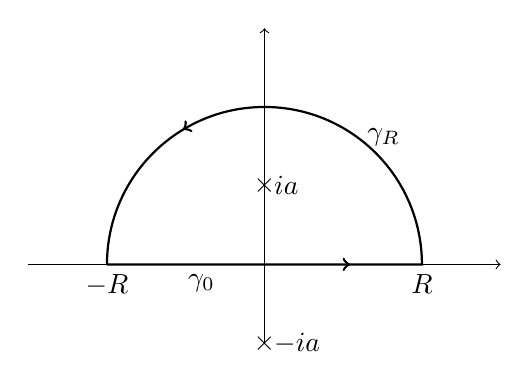
\begin{tikzpicture}
      \draw [->] (-3, 0) -- (3, 0);
      \draw [->] (0, -1) -- (0, 3);

      \draw [black, thick, ->-=0.3, ->-=0.8] (-2, 0) -- (2, 0) node [pos=0.3, below] {$\gamma_0$} arc(0:180:2) node [pos=0.3, right] {$\gamma_R$};

      \node [below] at (-2, 0) {$-R$};
      \node [below] at (2, 0) {$R$};

      \node at (0, 1) {$\times$};
      \node at (0, -1) {$\times$};
      \node [right] at (0, 1) {$ia$};
      \node [right] at (0, -1) {$-ia$};
    \end{tikzpicture}
  \end{center}
\item 
  We have 
  $$\int_{\gamma_R}\frac{e^{iz}}{a^2+z^2}dz=\int_0^\pi\frac{e^{iR\cos\theta-R\sin\theta}}{a^2+R^2e^{2i\theta}}iRe^{i\theta}d\theta$$
  which $\rightarrow 0$ as $R\rightarrow\infty$. Hence, $\int_C\frac{e^{iz}}{a^2+z^2}dz\rightarrow\int_{-\infty}^\infty\frac{e^{ix}}{a^2+x^2}dx$. Hence, looking at the real part,
  $$\int_{-\infty}^\infty\frac{\cos x}{a^2+x^2}dx=\frac{\pi}{a}e^{-a}$$
\end{enumerate}
\item
\begin{enumerate}[label=(\alph*)]
\item Write (**) as
$$\int_C\frac{1}{1+\epsilon(0.5)(z+z^{-1})}\frac{dz}{iz}=\int_C\frac{-2idz}{\epsilon z^2+2z+\epsilon}$$
where $C$ is a unit circle in the complex plane, traversing in the clockwise sense. 
\item 
The poles of the integrand are
$$\epsilon z^2+2z+\epsilon=0\implies z_{\pm}=\frac{-1\pm\sqrt{1-\epsilon^2}}{\epsilon^2}$$
These are first order zeros for the denominator, hence first order poles of the integrand. We have $\epsilon^2<1$, so $\sqrt{1-\epsilon^2}\in\mathbb{R}$ and hence
$z_-<-1$ and $z_+<0$. $z_+$ is enclosed in the unit circle even as $\epsilon\rightarrow 0$.
 \begin{center}
    \begin{tikzpicture}
      \draw [->] (-3, 0) -- (3, 0);
      \draw [->] (0, -3) -- (0, 3);
      \draw [black, thick, ->-=0.2,->-=0.7] circle [radius=1.8];
      \node [right] at (1.2726, 1.2726) {$\gamma$};

      \node (z-) at (-2.5, 0) {$\times$};
      \node [below] at (z-) {$z_-$};

      \node (z+) at (-1.2, 0) {$\times$};
      \node [below] at (z+) {$z_+$};
    \end{tikzpicture}
  \end{center}
\item The residue of $z_+$ is
$$\res_{z=z_+}\frac{-2i}{\epsilon(z-z_+)(z-z_-)}=\lim_{z\rightarrow z_+}\frac{-2i}{\epsilon(z-z_-)}=\frac{-2i}{\epsilon(z_+-z_-)}$$
By residue theorem,
$$\int_0^{2\pi}\frac{1}{1+\epsilon\cos\theta}d\theta=2\pi i\frac{-2i}{\epsilon(z_+-z_-)}=\frac{2\pi}{\sqrt{1-\epsilon^2}}$$
\end{enumerate}
\end{enumerate}
\end{ans}
\newpage
\begin{qns}[Transform Methods]\leavevmode
\begin{enumerate}[label=(\roman*)]
\item Calculate the Fourier transform of the triangle function\hfill\textbf{[5]}
\begin{equation}
   f(x)=
\left\{
        \begin{array}{ll}
      1-|x| & |x|<1 \\
      0 & \text{ otherwise}
        \end{array}
    \right.\tag{*} 
\end{equation}
The Fourier transform with respect to $x$ of a function $u(x, t)$ is given by
$$\tilde{u}(k,t)=\int_{-\infty}^\infty u(x,t)e^{-ikx}dx$$
\item Using the formal limit definition of a derivative, derive expressions for the Fourier transforms with respect to $x$ of $\frac{\partial u}{\partial t}$ and $\frac{\partial u}{\partial x}$. [Hint: You may assume that $u\rightarrow 0$ as $|x|\rightarrow\infty$.]\hfill\textbf{[5]}
\item If $u(x, t)$ satisfies
$$\frac{\partial^2u}{\partial t^2}=c^2\frac{\partial^2u}{\partial x^2}$$
write down the ordinary differential equation obeyed by the Fourier transform $\tilde{u}(k,t)$ of $u(x, t)$.\hfill\textbf{[4]}
\item Find $u(x, t)$ subject to the following initial conditions at $t = 0$
$$u=f(x),\quad \frac{\partial u}{\partial t}=0$$
where $f(x)$ is the triangle function. Assume again that $u\rightarrow 0$ as $|x|\rightarrow\infty$.\hfill\textbf{[6]}
\end{enumerate}
\end{qns}
\begin{ans}\leavevmode
\begin{enumerate}[label=(\roman*)]
\item The Fourier transform of (*) is
$$\tilde{f}=\int_{-1}^1(1-|x|)e^{-ikx}dx=2\int_0^1(1-x)\cos kx dx=\sinc^2(k/2)$$
\item Using limits,
$$\mathcal{F}\bigg[\frac{\partial u}{\partial t}\bigg]=\int_{-\infty}^\infty\lim_{\Delta t\rightarrow 0}\frac{u(x,t+\Delta t)-u(x,t)}{\Delta t}e^{-ikx}dx=\lim_{\Delta t\rightarrow 0}\frac{\tilde{u}(k,t+\Delta t)-\tilde{u}(k,t)}{\Delta t}=\frac{\partial\tilde{u}}{\partial t}$$
$$\mathcal{F}\bigg[\frac{\partial u}{\partial x}\bigg]=\int_{-\infty}^\infty\lim_{\Delta x\rightarrow 0}\frac{u(x+\Delta x,t)-u(x,t)}{\Delta x}e^{-ikx}dx=[ue^{-ikx}]_{-\infty}^\infty+ik\int_{-\infty}^\infty ue^{-ikx}dx$$
which is $ik\tilde{u}$ if we assume $u\rightarrow 0$ as $|x|\rightarrow\infty$.
\item The ODE is $\frac{\partial^2\tilde{u}}{\partial t^2}=-k^2c^2\tilde{u}$ for constant $u$.
\item The solution is $\tilde{u}(k,t)=A(k)e^{ikct}+B(k)e^{-ikct}$. From $\frac{\partial\tilde{u}}{\partial t}=0\implies A(k)=B(k)$ and $\tilde{u}=\tilde{f}(x)=A+B=2A\implies\mathcal{F}^{-1}[A]=\frac{1}{2}f(x)$. Writing the solution $u$ using inverse Fourier transform,
$$u(x,t)=\int_{-\infty}^\infty A(k)e^{i(ct+x)k}+B(k)e^{i(-ct+x)k}dk=\mathcal{F}^{-1}[A]+\mathcal{F}^{-1}[B]=\frac{1}{2}f(x+ct)+\frac{1}{2}f(x-ct)$$
From part (i), $f(x)$ is a triangle function, so the solution $u(x,t)$ consist of two triangular functions with half the height, one displaced to the left by a distance $ct$ and the another to the right by $ct$.
\end{enumerate}
\end{ans}
\newpage
\begin{qns}[Tensors]\leavevmode
\begin{enumerate}[label=(\roman*)]
\item State the transformation rules for tensors of rank one and two.\hfill\textbf{[2]}
\item If $u_i$ and $v_j$ are rank one tensors (i.e. vectors), show that $u_iv_j$ is a rank two tensor.\hfill\textbf{[2]}
\item Consider a rank two tensor $B_{ij}$. Let $S_{ij}$ and $A_{ij}$ be symmetric and anti-symmetric rank two tensors where $B_{ij} = S_{ij}+A_{ij}$. Write $S_{ij}$ and $A_{ij}$ in terms of the components of $B_{ij}$.\hfill\textbf{[2]}
\item Show that if $R_{ij}$ is a symmetric rank two tensor, then 
$$R_{ij}B_{ij}=R_{ij}S_{ij}$$
where $S_{ij}$ is the symmetric part of $B_{ij}$ defined above.\hfill\textbf{[2]}
\item Show that the tensor product of a rank two tensor with a vector is a rank three
tensor.\hfill\textbf{[2]}
\item Let $S_{ijk}$ be a rank three tensor. A contraction of $S_{ijk}$ is defined as
$$C_k=\sum_i S_{iik}$$
Show that $C_k$ is a vector.\hfill\textbf{[4]}
\item Using suffix notation and the Levi-Civita pseudo-tensor, $\epsilon_{ijk}$, prove the following vector identity\hfill\textbf{[6]}
$$\boldsymbol{\nabla}\times(\mathbf{A}\times\mathbf{B})=\mathbf{A}\boldsymbol{\nabla}\cdot\mathbf{B}+(\mathbf{B}\cdot\boldsymbol{\nabla})\mathbf{A}-\mathbf{B}\boldsymbol{\nabla}\cdot\mathbf{A}-(\mathbf{A}\cdot\boldsymbol{\nabla})\mathbf{B}$$
\end{enumerate}
\end{qns}
\begin{ans}\leavevmode
\begin{enumerate}[label=(\roman*)]
\item Transformation rule for tensor of rank one: $u_i'=L_{ij}u_j$ where $L_{ij}$ is an element of an orthogonal transformation ($LL^T=I$), relating two bases systems.\\[5pt]
Transformation rule for tensor of rank two: $B_{ij}'=L_{ia}L_{jb}B_{ab}$.
\item $(u_iv_j)'=L_{i\alpha}u_\alpha L_{j\beta}v_\beta=L_{i\alpha}L_{j\beta}(u_\alpha v_\beta)$, so it is rank-two tensor.
\item $S_{ij}=\frac{1}{2}(B_{ij}+B_{ji})$ and $A_{ij}=\frac{1}{2}(B_{ij}-B_{ji})$.
\item We note the contraction of a symmetric and anti-symmetric tensor gives:
$$R_{ij}A_{ij}=-R_{ij}A_{ji}=-R_{ij}A_{ij}\implies R_{ij}A_{ij}=0$$
where we used the definition of anti-symmetric tensor, followed by relabellign the dummy index.
\item $(A_{ij}v_k)'=L_{i\alpha}L_{j\beta}A_{\alpha\beta}L_{k\gamma}v_\gamma$, so it is rank-three tensor.
\item $C_k'=S_{iik}=L_{ia}L_{ib}L_{kc}S_{abc}=\delta_{ab}L_{kc}S_{abc}=L_{kc}S_{aac}$, where $L$ is orthogonal, i.e. $LL^T=I$, hence rank-one tensor, i.e. vector.
\item It is obvious both sides is a rank-one tensor.
$$\boldsymbol{\nabla}\times(\mathbf{A}\times\mathbf{B})=\epsilon_{ijk}\frac{\partial}{\partial x_i}\epsilon_{pqj}A_pB_q\mathbf{\hat{k}}=(\delta_{kp}\delta_{iq}-\delta_{kq}\delta_{ip})\frac{\partial}{\partial x_i}(A_pB_q)\mathbf{\hat{k}}$$
Expand the derivative by chain rule and expand everything. Finally, realize that $\boldsymbol{\nabla}\cdot\mathbf{V}=\frac{\partial V_i}{\partial x_i}$ and $\mathbf{V}\cdot\boldsymbol{\nabla}=V_i\frac{\partial}{\partial x_i}$ for an arbtirary vector field $\mathbf{V}(\mathbf{x})$.
\end{enumerate}
\end{ans}
\newpage
\begin{qns}[Normal Modes]
Two objects with masses $m_1$ and $m_2$ are connected to two rigid walls by three springs with identical spring constants $k$, as sketched below. Let $x_1$ and $x_2$ be the displacements of $m_1$ and $m_2$ from their equilibrium positions, respectively. The motion of the objects is confined to the horizontal ($x$) direction. 
\begin{figure}[H]
    \centering
    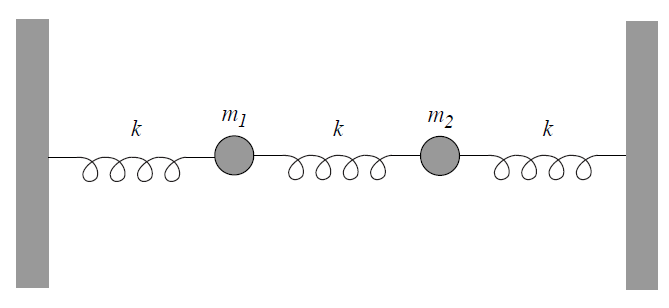
\includegraphics[scale=0.5]{2013P2Q7.PNG}
\end{figure}
\begin{enumerate}[label=(\roman*)]
\item Find the normal modes of oscillation and their associated frequencies.\hfill\textbf{[10]}
\item At $t = 0$, the masses are each displaced from their equilibrium position by a distance $x_0$ and away from each other, then released from a state of rest. Solve for $x_1$ and $x_2$ and express them as linear combinations of the normal modes.\hfill\textbf{[5]}
\item If the masses are initially at the equilibrium position, but $m_2$ is given an initial velocity $u_0$, while $m_1$ is initially at rest, solve for $x_1$ and $x_2$. Describe this motion in terms of the normal modes.\hfill\textbf{[5]}
\end{enumerate}
\end{qns}
\begin{ans}\leavevmode
\begin{enumerate}[label=(\roman*)]
\item The kinetic energy is
$$T=\frac{1}{2}m_1\dot{x}_1^2+\frac{1}{2}m_2\dot{x}_2^2=\frac{1}{2}\begin{pmatrix}\dot{x}_1&\dot{x}_2\\\end{pmatrix}\begin{pmatrix}m_1&0\\0&m_2\\\end{pmatrix}\begin{pmatrix}\dot{x}_1\\\dot{x}_2\\\end{pmatrix}:=\frac{1}{2}\mathbf{\dot{x}}^T\mathcal{T}\mathbf{\dot{x}}$$
and the potential energy is
$$V=\frac{1}{2}kx_1^2+\frac{1}{2}k(x_1-x_2)^2+\frac{1}{2}kx_2^2=\frac{1}{2}\begin{pmatrix}x_1&x_2\\\end{pmatrix}\begin{pmatrix}2k&-k\\-k&2k\\\end{pmatrix}\begin{pmatrix}x_1\\x_2\\\end{pmatrix}:=\frac{1}{2}\mathbf{x}^T\mathcal{V}\mathbf{x}$$
The Lagrangian is $\mathcal{L}=T-V=\frac{1}{2}\mathbf{\dot{x}}^T\mathcal{T}\mathbf{\dot{x}}-\frac{1}{2}\mathbf{x}^T\mathcal{V}\mathbf{x}$ and thus the Euler-Lagrange equation extremizes the Lagrangian to give $0=\frac{d}{dt}\frac{\partial\mathcal{L}}{\partial\mathbf{\dot{x}}}-\frac{\partial\mathcal{L}}{\partial\mathbf{x}}=\frac{d}{dt}(\mathcal{T}\mathbf{\dot{x}})+\mathcal{V}\mathbf{x}$. Since $T$ is time-independent, we can look for solutions of the form $\mathbf{x}(t)=\mathbf{A}e^{i\omega t}$:
$$0=\det(\mathcal{V}-\omega^2\mathcal{T})=\det\begin{pmatrix}2k-\omega^2m_1&-k\\-k&2k-\omega^2m_2\\\end{pmatrix}=3k^2-2k\omega^2(m_2+m_1)+\omega^4m_1m_2$$
Rearranging gives
$$\omega_\pm^2=k\frac{m_1+m_2}{m_1m_2}\pm\frac{k}{m_1m_2}\sqrt{m_1^2+m_2^2-m_1m_2}$$
Let the ratio of masses be $\alpha=\frac{m_1}{m_2}$, then
$$\frac{m_1}{k}\omega^2=(\alpha+1)\pm\sqrt{\alpha^2-\alpha+1}, \quad \frac{m_2}{k}\omega^2=1+\alpha^{-1}\pm\sqrt{\alpha^{-2}-\alpha^{-1}+1}$$
Let the eigenvector be $(a,b)^T$, then the first line of $(\mathcal{V}-\omega^2\mathcal{T})$ gives $$(2k-m_1\omega_+^2)a-kb=0\implies b=a(1-\alpha\pm\sqrt{\alpha^2-\alpha+1})$$ The normal modes are the unnormalized eigenvectors are $\mathbf{A_\pm}=(1,1-\alpha\pm\sqrt{\alpha^2-\alpha+1})^T$. Verify that these eigenvectors are orthogonal with respect to $\mathcal{T}$:
\begin{align}
\langle\mathbf{A_-}|\mathbf{A_+}\rangle_{\mathcal{T}}&=\begin{pmatrix}1&1-\alpha-\sqrt{\alpha^2-\alpha+1}\\\end{pmatrix}\begin{pmatrix}\alpha&0\\0&1\\\end{pmatrix}\begin{pmatrix}1\\1-\alpha+\sqrt{\alpha^2-\alpha+1}\\\end{pmatrix}\nonumber\\&=\alpha+(1-\alpha)^2-(\alpha^2-\alpha+1)\nonumber\\&=0\nonumber
\end{align}
\item The general solution is
$$\mathbf{x}(t)=\text{Re}[c_+e^{i\omega_+t}]\begin{pmatrix}1\\1-\alpha-\sqrt{\alpha^2-\alpha+1}\\\end{pmatrix}+\text{Re}[c_-e^{i\omega_-t}]\begin{pmatrix}1\\1-\alpha+\sqrt{\alpha^2-\alpha+1}\\\end{pmatrix}$$
The initial conditions are $\mathbf{x}(t=0)=(x_0,-x_0)^T$ and $\mathbf{\dot{x}}(t=0)=(0,0)^T$. We exploit orthogonality:
\begin{equation}
  \text{Re}[c_\pm]=\frac{\langle\mathbf{x}(0)|\mathbf{A_\pm}\rangle_{\mathcal{T}}}{\langle\mathbf{A_\pm}|\mathbf{A_\pm}\rangle_{\mathcal{T}}},\quad \text{Im}[-\omega_\pm c_\pm]=\frac{\langle\mathbf{\dot{x}}(0)|\mathbf{A_\pm}\rangle_{\mathcal{T}}}{\langle\mathbf{A_\pm}|\mathbf{A_\pm}\rangle_\mathcal{T}}\nonumber
\end{equation}
We have $\langle\mathbf{A}_\pm|\mathbf{A}_\pm\rangle_{\mathcal{T}}=2m_2(1-\alpha+\alpha^2\pm(1-\alpha)\sqrt{1-\alpha+\alpha^2})$. From $\mathbf{\dot{x}}(t=0)=(0,0)^T$, it is obvious that $c_\pm\in\mathbb{R}$,and so
$$c_\pm=\frac{x_0(-1+2\alpha\mp\sqrt{\alpha^2-\alpha+1})}{2(1-\alpha+\alpha^2\pm(1-\alpha)\sqrt{1-\alpha+\alpha^2})}$$
Hence, the solution is 
$$\mathbf{x}(t)=c_+\cos(\omega_+t)\begin{pmatrix}1\\1-\alpha-\sqrt{\alpha^2-\alpha+1}\\\end{pmatrix}+c_-\cos(\omega_-t)\begin{pmatrix}1\\1-\alpha+\sqrt{\alpha^2-\alpha+1}\\\end{pmatrix}$$
\item Now, the initial conditions are $\mathbf{x}(t=0)=(0,0)^T$ and $\mathbf{\dot{x}}(0)=(0,u_0)^T$. This time, $c_\pm$ is purely imaginary.
$$c_\pm=\frac{-1}{\omega_\pm}\frac{u_0(1-\alpha\pm\sqrt{\alpha^2-\alpha+1})}{2(1-\alpha+\alpha^2\pm(1-\alpha)\sqrt{1-\alpha+\alpha^2})}$$
Hence the solution is $$\mathbf{x}(t)=-c_+\sin(\omega_+t)\begin{pmatrix}1\\1-\alpha-\sqrt{\alpha^2-\alpha+1}\\\end{pmatrix}-c_-\sin(\omega_-t)\begin{pmatrix}1\\1-\alpha+\sqrt{\alpha^2-\alpha+1}\\\end{pmatrix}$$
\end{enumerate}
\end{ans}
\begin{qns}[Group Theory]\leavevmode
\begin{enumerate}[label=(\roman*)]
\item Consider the set of functions of $x$
$$\mathcal{F}=\bigg\{x,-x,\frac{1}{x},-\frac{1}{x}\bigg\}$$
endowed with the operation of functional composition, i.e. if $f,g\in\mathcal{F}$ then $f *g = f(g(x))$.
\begin{enumerate}[label=(\alph*)]
\item Prove that $\mathcal{F}$ is a group. Construct a ‘multiplication’ table as part of your answer.\hfill\textbf{[6]}
\item What are the subgroups of $\mathcal{F}$?\hfill\textbf{[2]}
\item Prove that $\mathcal{F}$ is isomorphic to the dihedral group $D_2$.\hfill\textbf{[2]}
\end{enumerate}
\item State Lagrange’s theorem. Subsequently show that if the order of a group is prime then that group has no proper subgroups.\hfill\textbf{[3]}
\item Define the order of a group element. Prove that the order of any group element is a factor of the group’s order.\hfill\textbf{[3]}
\item Show that if the order of a group is prime then that group is cyclic.\hfill\textbf{[2]}
\item Suppose $\mathcal{G}$ is a cyclic group but not of prime order. Demonstrate that $\mathcal{G}$ contains a
proper cyclic subgroup.\hfill\textbf{[2]}
\end{enumerate}
\end{qns}
\newpage
\begin{ans}\leavevmode
\begin{enumerate}[label=(\roman*)]
\item 
\begin{enumerate}[label=(\alph*)]
\item The multiplication table of $\mathcal{F}$ is
$$\vbox{\tabskip0.5em\offinterlineskip
    \halign{\strut$#$\hfil\ \tabskip1em\vrule&&$#$\hfil\cr
    ~   & x & -x &1/x&-1/x \cr
    \noalign{\hrule}\vrule height 12pt width 0pt
    x & x & -x &1/x&-1/x \cr
    -x & -x & x &-1/x & 1/x \cr
    1/x & 1/x & -1/x & x &-x \cr
    -1/x & -1/x &1/x & -x & x\cr
}}$$
Check the group axioms:
\begin{itemize}
    \item Closure: yes, see the group table.
    \item Associativity: functional composition is associative
    $$(f*g)*h=(f*g)(h(x))=f(g)(h(x))=f((g*h))(x)=f*(g*h)$$
    \item Identity: $x$ is the identity;
    \item Inverse: each element in $\mathcal{F}$ is its own inverse.
\end{itemize}
\item The trivial subgroup and $\mathcal{F}$ itself are subgroups of $\mathcal{F}$. The remaining subgroups are proper: $\{x,-x\}$, $\{x,1/x\}$.
\item The dihedral group of a rectangle contains $r$ (rotations by $\pi$) and $s$ (reflection) where $r^2=\Id=s^2$. It also contains $rs$ where $rsrs=rssr^{-1}=\Id$. The map $\Phi:~\mathcal{F}\rightarrow D_2$ thus
$$x\mapsto\Id,\quad -x\mapsto r,\quad 1/x\mapsto s,\quad -1/x\mapsto rs$$
This map is bijective (easy to check). It is also a homomorphism, for instance $\Phi(-1/x)=\Phi(-x)\Phi(1/x)=rs$. Thus, it is an isomorphism.
\end{enumerate}
\item Lagrange's theorem states that the order of $H\leq G$ is such that $\frac{|G|}{|H|}\in\mathbb{N}$. Since the only divisors of a prime number are itself and one, and the subgroups of these orders are the entire group and the trivial subgroup (contains just the identity). hence, the group has no proper subgroup.
\item The order of a group element $g\in G$ is the smallest $k\in\mathbb{N}$ such that $g^k=e$. Write as $\ord(g)=k$. The resultant group generated is $\langle g\rangle=\{g,g^2,\dots,g^{k-1},e\}$. $\langle g\rangle\leq G$ because
\begin{itemize}
    \item Closure: $g^sg^r=g^{p}$ where $p=(s+r)\text{ mod}k$.
    \item Associativity: inherited;
    \item Identity: the same as that of $G$;
    \item Inverse: $g^{k-r}$ is the inverse of $g^r$.
\end{itemize}
By Lagrange's theorem, $\ord(g)$ divides $|G|$.
\item $|G|=p$ prime. Take $g\in G$ but $g\neq e$, so $\ord(g)=p$. Hence, $\langle g\rangle=G$, i.e. cyclic.
\item If $\mathcal{G}$ is cyclic s.t. $|\mathcal{G}|=nm$ with $n,m\in\mathbb{Z}$ but $n,m\neq 1$. Take $g\in\mathcal{G}$ s.t. $|g|=nm$, then $\exists h\in\mathcal{G}$ s.t. $g^n=h$ where $|h|=m$ which generates a cyclic subgroup of order $m<p$, i.e. a proper cyclic subgroup.
\end{enumerate}
\end{ans}
\newpage
\begin{qns}[Group Theory]\leavevmode
\begin{enumerate}[label=(\roman*)]
\item What is meant by the terms normal subgroup and group homomorphism?\hfill\textbf{[2]}
\item Consider the group homomorphism $\phi:\mathcal{G}_1\rightarrow\mathcal{G}_2$.
\begin{enumerate}[label=(\alph*)]
\item Prove that the image of $\phi$ is a subgroup of $\mathcal{G}_2$.\hfill\textbf{[2]}
\item Prove that the kernel $K$ of $\phi$ is a normal subgroup of $\mathcal{G}_1$.\hfill\textbf{[3]}
\item Demonstrate that if $K$ consists only of the identity element then $\phi$ is injective (i.e. one-to-one).\hfill\textbf{[3]}
\end{enumerate}
\item
\begin{enumerate}[label=(\alph*)]
\item If $D_3$ is the symmetry group of the equilateral triangle, describe the geometrical action of the six members of $D_3$ and give the minimal generating set of the group. Express the members of $D_3$ in terms of the generators.\hfill\textbf{[6]}
\item Identify the members of $D_3$ with the permutation group $\Sigma_3$. Hence show that the two groups are isomorphic.\hfill\textbf{[4]}
\end{enumerate}
\end{enumerate}
\end{qns}
\begin{ans}\leavevmode
\begin{enumerate}[label=(\roman*)]
\item $H\leq G$ is a normal subgroup if for every $h\in H$ and $g\in G$, we have $ghg^{-1}\in H$.\\[5pt]
$\phi$ is a group homomorphism if $\forall a,b\in H$, then
$$\phi(a\cdot_H b)=\phi(a)\cdot_G\phi(b)$$
\item 
\begin{enumerate}[label=(\alph*)]
\item Check subgroup axioms:
\begin{itemize}
    \item Closure: $\forall g_1,g_2\in \mathcal{G}_1\implies g_1g_2\in\mathcal{G}_1$ (since $\mathcal{G}_1$ is a group), then $$\phi(g_1)\phi(g_2)=\phi(g_1g_2)\in \mathcal{G}_2$$
    \item Associativity: inherits from $\mathcal{G}_2$;
    \item Identity: same as that of $\mathcal{G}_2$;
    \item Inverse: $\forall g\in\mathcal{G}_1$, $\exists g^{-1}\in\mathcal{G}_1$ such that
    $$\phi(e)=\phi(g^{-1}g)=\phi(g^{-1})\phi(g)\implies(\phi(g))^{-1}=\phi(g^{-1})\in\mathcal{G}_2$$
\end{itemize}
\item First check subgroup axioms for $K$:
\begin{itemize}
    \item Closure: $\forall g_1,g_2\in K$, $e=\phi(g_1)\phi(g_2)=\phi(g_1g_2)\implies g_1g_2\in K$;
    \item Associativity: inherited from $\mathcal{G}_1$;
    \item Identity: Same identity as that of $\mathcal{G}_1$ $$\phi(e_{\mathcal{G}_1}\in\mathcal{G}_1)=e_{\mathcal{G}_2}\implies e_{\mathcal{G}_1}\in K$$
    \item Inverse: For $g\in K$,
    $$e=\phi(e)=\phi(g^{-1}g)=\phi(g^{-1})\phi(g)=e\phi(g^{-1})\implies\phi(g^{-1})=e\implies g^{-1}\in K$$
\end{itemize}
Let $k\in K$, then $\phi(k)=e$. If $g\in\mathcal{G}_1$,
$$\phi(gkg^{-1})=\phi(g)\phi(k)\phi(g^{-1})=\phi(e)=e\implies gkg^{-1}\in K\implies K\lhd\mathcal{G}_1$$
\item Suppose the contrary. If $g\neq e_{\mathcal{G}_1}$ and $g\in K$, then $\phi(g)=e_{\mathcal{G}_2}$, so both $e_{\mathcal{G}_1}$ and $g$ map to $e_{\mathcal{G}_2}$, i.e. not one-to-one.
\end{enumerate}
\item 
\begin{enumerate}[label=(\alph*)]
\item $D_3$ contains $r$ (rotation by $2\pi/3$) and $s$ (reflection about a line passing through one vertex and the centre), then 
$$D_3=\{\Id,r,r^2,s,sr,sr^2\},\quad sr=r^2s$$
The generators are $\langle r\rangle=\{r,r^2,\Id\}=\langle r^2\rangle\implies\ord(r)=\ord(r^2)=3$, $\langle s\rangle=\{s,\Id\}$, $\langle sr\rangle=\{sr,srsr=srr^2s=\Id\}$ and $\langle sr^2\rangle=\{sr^2,sr^2sr^2=sr^2rs=\Id\}$. Hence, $\ord(s)=\ord(sr)=\ord(sr^2)=2$. Trivially, $\langle\Id\rangle=\{\Id\}$ so $\ord(\Id)=1$.
\item We can construct the mapping $\Phi$ such that
$$\Id\mapsto(1)(2)(3),~ r\mapsto(123),~r^2\mapsto(321),~s\mapsto(12),sr\mapsto(13),~sr^2\mapsto(23)$$
We can easily check that it is a homomorphism. Also check commutation: $srs=(12)(123)(12)=(12)(13)=(321)=r^2$, i.e. preserved. $\Phi$ is one-to-one and onto. Thus, $\Phi$ is an isomorphism, i.e. $D_3\simeq\Sigma_3$.
\end{enumerate}
\end{enumerate}
\end{ans}
\newpage
\begin{qns}[Representation Theory]\leavevmode
\begin{enumerate}[label=(\roman*)]
\item Define faithful representation, equivalent representations, irreducible representation, and the character of a representation.\hfill\textbf{[4]}
\item Let $\mathcal{G}$ be the following set of real $4\times 4$ matrices
$$\begin{pmatrix}1&0&0&0\\0&1&0&0\\0&0&1&0\\0&0&0&1\\\end{pmatrix},\quad\begin{pmatrix}0&1&0&0\\1&0&0&0\\0&0&0&1\\0&0&1&0\\\end{pmatrix},\quad\begin{pmatrix}0&0&1&0\\0&0&0&1\\1&0&0&0\\0&1&0&0\\\end{pmatrix},\quad\begin{pmatrix}0&0&0&1\\0&0&1&0\\0&1&0&0\\1&0&0&0\\\end{pmatrix}$$
\begin{enumerate}[label=(\alph*)]
\item Show that $\mathcal{G}$ is a group under the operation of matrix multiplication. Go on to show that it is a faithful representation of the dihedral group $D_2$.\hfill\textbf{[5]}\item By finding an invariant subspace of the representation, prove that $\mathcal{G}$ is reducible.\hfill\textbf{[3]}
\end{enumerate}
\item 
\begin{enumerate}[label=(\alph*)]
\item What are the conjugacy classes of $Z_n$, the cyclic group of order $n$? What can you say about the number and dimensions of its irreducible representations? \hfill\textbf{[4]}
\begin{mdframed}
\textcolor{darkblue}{Hint: You may need the result $|\mathcal{G}|=\sum_{k=1}^{n_p}d_k^2$, where $n_p$ is the number of irreducible representations of any group $\mathcal{G}$ and $d_k$ is the dimension of the $k$’th representation.}
\end{mdframed}
\item Give the irreducible representations of $Z_n$. Write down the associated character table for the special case $n = 3$.\hfill\textbf{[4]}
\end{enumerate}
\end{enumerate}
\end{qns}
\begin{ans}\leavevmode
\begin{enumerate}[label=(\roman*)]
\item The definitions:
\begin{itemize}
    \item A faithful representation is one where each element in the representation only has one pre-image.
    \item Two representations $D_1(G)$ and $D_2(G)$ are equivalent if $\exists$ some matrix $S$ s.t. $SD_1(g_i)S^{-1}=D_2(g_i)$ $\forall g_i\in G$.
    \item An irreducible representation is one where a single similarity transformation $S$ cannot be found such that $SD(g_i)S^{-1}$ is a diagonal matrix $\forall g_i\in G$ simultaneously.
    \item The character of a representation is the vector of the traces of the matrices representing the individual elements.
\end{itemize}
\item 
\begin{enumerate}[label=(\alph*)]
\item Check group axioms:
\begin{itemize}
    \item Closure: 
    $$\begin{pmatrix}0&1&0&0\\1&0&0&0\\0&0&0&1\\0&0&1&0\\\end{pmatrix}\begin{pmatrix}0&0&1&0\\0&0&0&1\\1&0&0&0\\0&1&0&0\\\end{pmatrix}=\begin{pmatrix}0&0&0&1\\0&0&1&0\\0&1&0&0\\1&0&0&0\\\end{pmatrix}$$
    $$\begin{pmatrix}0&1&0&0\\1&0&0&0\\0&0&0&1\\0&0&1&0\\\end{pmatrix}\begin{pmatrix}0&0&0&1\\0&0&1&0\\0&1&0&0\\1&0&0&0\\\end{pmatrix}=\begin{pmatrix}0&0&1&0\\0&0&0&1\\1&0&0&0\\0&1&0&0\\\end{pmatrix}$$
    $$\begin{pmatrix}0&0&0&1\\0&0&1&0\\0&1&0&0\\1&0&0&0\\\end{pmatrix}\begin{pmatrix}0&0&1&0\\0&0&0&1\\1&0&0&0\\0&1&0&0\\\end{pmatrix}=\begin{pmatrix}0&1&0&0\\1&0&0&0\\0&0&0&1\\0&0&1&0\\\end{pmatrix}$$
    \item Associativity: matrix multiplication is associative;
    \item Identity: $I_{4\times 4}$;
    \item Inverse: Each matrix is its own inverse.
\end{itemize}
The faithful representation of $D_2$ is $\{\Id,r,s,rs\}$ since each of the 3 non-identity matrix can be mapped bijectively to $r$, $s$ and $rs$.
\item By inspection, the invariant subspace is $(1,1,1,1)^T$ since the matrix are formed by permutating the rows/columns of the identity. Hence, $\exists$ a similarity transformation which will put all four matrix into the form $1\oplus A_{3\times 3}$.
\end{enumerate}
\item 
\begin{enumerate}[label=(\alph*)]
\item 
For an element $g_i\in Z_n$ to be conjugate to another element $g_j$, then $\exists z\in Z_n$ s.t. $zg_jz^{-1}=g_i$, but all elements of a cyclic group can be expressed as a single generator $f\in Z_n$ to some power $p\leq n$, i.e. $z=f^r$, $z^{-1}=f^q$, then
$$zg_iz^{-1}=f^rf^if^q=f^{r+q}f^i=f^i~\forall i$$
Each element is thus a conjugate class of its own.\\[5pt]
Since we are given that the number of distinct irreducible representations is equal to the number of conjugate classes, then there are a total of $n$ one-dimensional irreducible representations of $Z_n$ since each of the $n$ elements form a distinct conjugate class of its own.
\item 
The irreducible representations of $Z_n$ are generated by $e^{i2\pi n/p}\in\mathbb{C}$ (one-dimensional) where $p\in\{1,\dots,n\}$. For $n=3$ and recalling for one-dimensional representations, the trace is just itself, then the associated character table is
\begin{center}
\begin{tabular}{ |c|c|c|c| } 
\hline
   Rep 1 & 1 &1 &1\\
   \hline
   Rep 2 & 1 &$e^{2\pi i/3}$ & $e^{4\pi i/3}$\\
   \hline
   Rep 3 & 1 & $e^{4\pi i/3}$ & $e^{2\pi i/3}$\\
 \hline
\end{tabular}
\end{center}
which does satisfy the character orthogonality theorem, by noting $1+e^{2\pi i/3}+e^{4\pi i/3}=0$ since they are roots of a quadratic equation $x^2+x+1=0$.
\end{enumerate}
\end{enumerate}
\end{ans}
\newpage
\section{2014}
\subsection{Paper 1}
\begin{qns}[Vector Calculus]\leavevmode
\begin{enumerate}[label=(\roman*)]
    \item  Using Cartesian coordinates show that
$$\boldsymbol{\nabla}\times(\boldsymbol{\nabla}\times\mathbf{u})=\boldsymbol{\nabla}(\boldsymbol{\nabla}\cdot\mathbf{u})-\nabla^2\mathbf{u}$$
and that
$$\boldsymbol{\nabla}\times(\mathbf{u}\times\mathbf{v})=\mathbf{u}(\boldsymbol{\nabla}\cdot\mathbf{v})-\mathbf{v}(\boldsymbol{\nabla}\cdot\mathbf{u})+(\mathbf{v}\cdot\boldsymbol{\nabla})\mathbf{u}-(\mathbf{u}\cdot\boldsymbol{\nabla})\mathbf{v}$$
where $\mathbf{u}$ and $\mathbf{v}$ are three-dimensional vector fields.\hfill \textbf{[6]}
\item State the divergence theorem and use it to show that
$$\int_V[\mathbf{G}\cdot(\boldsymbol{\nabla}\times\mathbf{F})-\mathbf{F}\cdot(\boldsymbol{\nabla}\times\mathbf{G})]dV=\int_S(\mathbf{F}\times\mathbf{G})\cdot\mathbf{\hat{n}}dS$$
where $\mathbf{F}$ and $\mathbf{G}$ are three-dimensional vector fields, $V$ is a given volume with surface $S$, and $\mathbf{\hat{n}}$ is the outward unit vector normal to $S$.\hfill \textbf{[6]}
\item Let $V$ be the volume bounded by the plane $z = 0$ and the paraboloid $z = 4−x^2−y^2$ with surface $S$ and outward unit normal vector $\mathbf{\hat{n}}$. If
$$\mathbf{F}=\begin{pmatrix}xz\sin(yz)+x^3\\\cos(yz)\\3zy^2-e^{x^2+y^2}\\\end{pmatrix}$$
find $\int_S\mathbf{F}\cdot\mathbf{\hat{n}}dS$.\hfill \textbf{[8]}
\end{enumerate}
\end{qns}
\begin{ans}\leavevmode
\begin{enumerate}[label=(\roman*)]
    \item Use suffix notation in Cartesian coordinates for LHS of both identities:
$$\epsilon_{ijk}\frac{\partial}{\partial x_i}(\boldsymbol{\nabla}\times\mathbf{u})_j=\epsilon_{kij}\epsilon_{pqj}\frac{\partial}{\partial x_i}\frac{\partial}{\partial x_p}u_q=\frac{\partial^2u_i}{\partial x_k\partial x_i}-\frac{\partial^2u_k}{\partial x_i\partial x_i}$$
$$\epsilon_{ijk}\frac{\partial}{\partial x_i}(\mathbf{u}\times\mathbf{v})_j=\epsilon_{kij}\epsilon_{pqj}\frac{\partial}{\partial x_i}u_pv_q=\frac{\partial}{\partial x_i}(u_kv_i)-\frac{\partial}{\partial x_i}(u_iv_k)=u_k\frac{\partial v_i}{\partial x_i}+v_i\frac{\partial u_k}{\partial x_i}-v_k\frac{\partial u_i}{\partial x_i}-u_i\frac{\partial v_k}{\partial x_i}$$
\item If $\mathbf{F}=\mathbf{F}(\mathbf{x})$ be a continuously differentiable vector field and $V$ is a volume with a piecewise regular boundary $\partial V$, then the divergence theorem states
$$\int_V\boldsymbol{\nabla}\cdot\mathbf{F}dV=\int_{\partial V}\mathbf{F}\cdot d\mathbf{S}$$
where the normal to $\partial V$ points outwards from $V$. RHS of our desired result is $\int_V\boldsymbol{\nabla}\cdot(\mathbf{F}\times\mathbf{G})dV$ after invoking divergence theorem. Then, using suffix notation again. The result follows after a volume integral.
$$\frac{\partial}{\partial x_k}\epsilon_{ijk}F_iG_j=-\epsilon_{kji}\frac{\partial G_j}{\partial x_k}F_i+\epsilon_{kij}\frac{\partial F_i}{\partial x_k}G_j\implies\boldsymbol{\nabla}\cdot(\mathbf{F}\times\mathbf{G})=-(\boldsymbol{\nabla}\times\mathbf{G})\cdot\mathbf{F}+(\boldsymbol{\nabla}\times\mathbf{F})\cdot\mathbf{G}$$ 
\item We invoke Divergence Theorem again and evaluate $\boldsymbol{\nabla}\cdot\mathbf{F}=3(x^2+y^2)$. We change to cylindrical coordinates, $z\in[0,4-r^2]$ and $r\in[0,2]$ such that
$$\int_S\mathbf{F}\cdot\mathbf{n}dS=\int_{S\cup C}\mathbf{F}\cdot\mathbf{n}dS-\int_C\mathbf{F}\cdot\mathbf{n}dS=\int_V(\boldsymbol{\nabla}\cdot\mathbf{F})dV-\int_C\mathbf{F}\cdot\mathbf{n}dS$$
where $C$ is a circular disc at $z=0$ plane, oriented such that $\mathbf{n}=(0,0,-1)^T$. In that case, $\int_C\mathbf{F}\cdot\mathbf{n}dS=\int_0^{2\pi}\int_0^2 r(e^{r^2}-3zr^2\sin^2\theta)drd\theta=\pi(e^4-1)$. We thus have
$$\int_S\mathbf{F}\cdot\mathbf{n}dS=32\pi-\pi(e^4-1)=(33-e^4)\pi$$
\end{enumerate}
\end{ans}
\newpage
\begin{qns}[Partial Differential Equation]
The velocity, $u(x, t)$, of a viscous fluid satisfies
\begin{equation}
\frac{\partial u}{\partial t}=\nu\frac{\partial^2u}{\partial x^2}\tag{*}
\end{equation}
where $\nu$ is a positive constant.
\begin{enumerate}[label=(\roman*)]
    \item Consider the flow of a semi-infinite viscous fluid above a flat oscillating plate with boundary conditions $u(0,t)=U_0\cos(\omega t)$ and $\lim_{x\rightarrow\infty}u(x,t)=0$. Using the method of separation of variables, solve for $u(x, t)$.\hfill \textbf{[10]}\\[5pt]
[Hint: Consider the complex velocity, $v$, such that $u = \Re(v)$ where $\Re$ denotes the real part.]
\item  A viscous fluid satisfying (*) is confined between two stationary parallel plates, separated by a distance $L$. At t = 0, the fluid velocity is
$$u(x,0)=U_0\bigg(\frac{x}{L}-\frac{x^2}{L^2}\bigg)$$
and the fluid remains at rest at each plate with boundary conditions $u(0,t)=0$ and $u(L,t)=0$ for $t\geq0$. Using the method of separation of variables, find a series solution for the velocity $u(x, t)$ for $t\geq0$. Write down an expression for the series coefficients. What is the velocity in the limit as $t\rightarrow\infty$?\hfill \textbf{[10]}
\end{enumerate}
\end{qns}
\begin{ans}\leavevmode
\begin{enumerate}[label=(\roman*)]
    \item We solve by separation of variables, $v(x,t)=X(x)T(t)$ where $u=\Re(v)$. Then $$\frac{T'}{T}=\nu\frac{X''}{X}=\alpha\in\mathbb{C}$$
Given the form of $u(0,t)=U_0\cos(\omega t)$, $T$ has the form $e^{\alpha t}$. This boundary condition suggests $\alpha$ is a purely imaginary term, i.e. $\alpha=\pm ia^2\nu$, such that $\sqrt{\alpha/\nu}=\pm\sqrt{\pm i}a=\pm a\frac{1}{\sqrt{2}}(1\pm i)$. With $\lim_{x\rightarrow\infty}u(x,t)=0$, we can only have the following form for $u(x,t)$:
\begin{eqnarray}
u(x,t)&=&\text{Re}\bigg[\int_0^\infty\bigg(Ae^{-a(1+i)x/\sqrt{2}}+Be^{-a(1-i)x/\sqrt{2}}\bigg)e^{\pm ia^2\nu t}da\bigg]\nonumber\\&=&\int_0^\infty e^{-ax/\sqrt{2}}\bigg[A\cos(a^2\nu t-(ax/\sqrt{2}))+B\sin(a^2\nu t-(ax/\sqrt{2}))\bigg]da\nonumber
\end{eqnarray}
Imposing the boundary condition $U_0\cos(\omega t)=u(0,t)=\int_0^\infty A\cos(a^2\nu t)+B\sin(a^2\nu t)da$, then $a^2\nu=\omega$ and hence the general solution is
$$u(x,t)=U_0e^{-x\sqrt{\omega/2\nu}}\cos(\omega t-x\sqrt{\omega/2\nu})$$
\item  The fluid is constrained between $x=0$ and $x=L$ such that $u(0,t)=u(L,t)=0$, then
$$\frac{X''}{X}\nu=\frac{T'}{T}=-\lambda^2\nu,\lambda\in\mathbb{R}$$
such that $X=c_1\sin(\lambda x)+c_2\cos(\lambda x)$ where $\lambda=\frac{n\pi}{L}$ and $T\sim e^{-\nu n^2\pi^2t/L^2}$. From the boundary conditions, $c_2=0$  The general form of $u(x,t)$ is thus $\sum_{n=1}^\infty A_n\sin(\frac{n\pi x}{L})e^{-\nu n^2\pi^2t/L^2}$. We have
$$A_n=\frac{2}{L}\int_0^LU_0\bigg(\frac{x}{L}-\frac{x^2}{L^2}\bigg)\sin\frac{n\pi x}{L}dx=\frac{2}{L}\bigg[U_0\bigg(\frac{x}{L}-\frac{x^2}{L^2}\bigg)\frac{-L\cos(n\pi x/L)}{n\pi}\bigg]_0^L+\frac{2U_0}{n\pi}\int_0^L\bigg(\frac{1}{L}-\frac{2x}{L^2}\bigg)\cos\frac{n\pi x}{L}dx$$
which further simplifies to $A_n=\frac{4U_0L}{n^3\pi^3}$ for odd $n$ and 0 for even $n$. Hence,
$$u(x,t)=\sum_{p=0}^\infty\frac{4U_0L}{(2p+1)^3\pi^3}\sin\frac{(2p+1)\pi x}{L}e^{-\nu\pi^2t(2p+1)^2/L^2}$$
As $t\rightarrow\infty$, the slowest decaying exponential dominates.
$$u(x,t)\approx\frac{4U_0L}{\pi^3}\sin\frac{\pi x}{L}e^{-\nu\pi^2t/L^2}$$
\end{enumerate}
\end{ans}
\newpage
\begin{qns}[Green's Functions]
A beam lies along the $x$-axis with its ends at $x = 0$ and $x = 1$. The transverse displacement $y(x)$ of the beam when a force per length $f(x)$ is applied satisfies
$$\frac{d^4y}{dx^4}=f(x)$$
The boundary conditions are $y = 0$ and $\frac{dy}{dx}=0$ at both $x = 0$ and $x = 1$. The displacement can be written in terms of a Green’s function $G(x,\xi)$ as
$$y(x)=\int_0^1G(x,\xi)f(\xi)d\xi$$
\begin{enumerate}[label=(\roman*)]
    \item What conditions must the Green’s function satisfy at $x = 0$ and $x = 1$ and at $x=\xi$?\hfill \textbf{[4]}
    \item Construct the Green’s function to show that\hfill \textbf{[12]}
$$G(x,\xi)=
\left\{
        \begin{array}{ll}
      -\frac{1}{6}x^2(\xi-1)^2(x+2x\xi-3\xi) & \text{ for }x<\xi \\
      -\frac{1}{6}\xi^2(x-1)^2(\xi+2x\xi-3x) & \text{ for } x>\xi
        \end{array}
    \right.$$
    \item Consider two points $x_1$ and $x_2$ along the beam. A force $f(x) =\delta (x − x_1)$ causes a
displacement $y_1(x_2)$ at $x_2$. If the force is instead $f(x) = \delta(x−x_2)$, the displacement at $x_1$ is $y_2(x_1)$. Show that $y_1(x_2) = y_2(x_1)$. \hfill \textbf{[4]}
\end{enumerate}
\end{qns}
\begin{ans}\leavevmode
\begin{enumerate}[label=(\roman*)]
    \item The corresponding Green's function satisfy
    $$\frac{\partial^4G(x,\xi)}{\partial x^4}=\delta(x-\xi),\quad G(0,\xi)=G(1,\xi)=0,~G'(0,\xi)=G'(1,\xi)=0$$
    Integrate this over an infinitesimal region around $x=\xi$, then $G,G',G''$ must all be continuous everywhere including $x=\xi$ (otherwise $G'''\propto$ higher derivatives of $\delta(x-\xi)$, which is a contradiction). $G'''$ is continuous everywhere except at $x=\xi$ (unit jump discontinuity).
    \item We propose a polynomial solution (of order 3) for the Green's function
    $$G(x,\xi)=
    \left\{
        \begin{array}{ll}
      c_1x^3+c_2x^2+c_3x+c_4 & 0\leq x<\xi\leq 1 \\
      c_5x^3+c_6x^2+c_7x+c_8 & 0\leq \xi<x\leq 1
        \end{array}
    \right.$$
    $$\implies\frac{\partial G(x,\xi)}{\partial x}=
    \left\{
        \begin{array}{ll}
      3c_1x^2+2c_2x+c_3 & 0\leq x<\xi\leq 1 \\
      3c_5x^2+2c_6x+c_7 & 0\leq \xi<x\leq 1
        \end{array}
    \right.$$
    $$\implies\frac{\partial^2G(x,\xi)}{\partial x^2}=
    \left\{
        \begin{array}{ll}
      6c_1x+2c_2 & 0\leq x<\xi\leq 1 \\
      6c_5x+2c_6 & 0\leq \xi<x\leq 1
        \end{array}
    \right.$$
    $$\implies\frac{\partial^3G(x,\xi)}{\partial x^3}=
    \left\{
        \begin{array}{ll}
      6c_1 & 0\leq x<\xi\leq 1 \\
      6c_5 & 0\leq \xi<x\leq 1
        \end{array}
    \right.$$
    We require 8 equations for 8 unknowns. The first two is obtained from boundary conditions $G=0$ and $\frac{\partial G}{\partial x}=0$ at $x=0$ and $x=1$:
$$c_4=0;\quad  c_5+c_6+c_7+c_8=0$$
$$c_3=0;\quad  3c_5+2c_6+c_7=0$$
The next six is obtained from continuity conditions and discontinuity condition at $x=\xi$:
$$3\xi(c_5-c_1)=c_2-c_6;\quad6(c_5-c_1)=1$$
$$3(c_5-c_1)\xi^2+2(c_6-c_2)\xi+c_7-c_3=0;\quad(c_5-c_1)\xi^3+(c_6-c_2)\xi^2+(c_7-c_3)\xi+(c_8-c_4)=0$$
This gives the matrix equation:
$$\begin{pmatrix}-1&0&1&0&0&0\\0&0&1&1&1&1\\0&0&3&2&1&0\\0&1&0&-1&0&0\\-\xi^3&-\xi^2&\xi^3&\xi^2&\xi&1\\-3\xi^2&-2\xi&3\xi^2&2\xi&1&0\\\end{pmatrix}\begin{pmatrix}c_1\\c_2\\c_5\\c_6\\c_7\\c_8\\\end{pmatrix}=\begin{pmatrix}1/6\\0\\0\\\xi/2\\0\\0\\\end{pmatrix}\implies\begin{pmatrix}c_1\\c_2\\c_5\\c_6\\c_7\\c_8\\\end{pmatrix}=\begin{pmatrix}\frac{1}{6}(-1+3\xi^2-2\xi^3)\\\frac{1}{2}(\xi-2\xi^2+\xi^3)\\\frac{1}{6}(3\xi^2-2\xi^3)\\\frac{1}{2}(-2\xi^2+\xi^3)\\\xi^2/2\\-\xi^3/6\\\end{pmatrix}$$
hence
$$G(x,\xi)=
\left\{
        \begin{array}{ll}
      \frac{1}{6}(-1+3\xi^2-2\xi^3)x^3+\frac{1}{2}(\xi-2\xi^2+\xi^3)x^2 & 0\leq x<\xi\leq 1 \\
      \frac{1}{6}(3\xi^2-2\xi^3)x^3+\frac{1}{2}(-2\xi^2+\xi^3)x^2+\frac{1}{2}\xi^2x-\frac{1}{6}\xi^3& 0\leq \xi<x\leq 1
        \end{array}
    \right.$$
which simplifies to their desired result.
\item To show $y_1(x_2)=y_2(x_1)$, we need to show the associated Green's functions for a self-adjoint operator $\mathcal{L}$ (in this case $\mathcal{L}=y^{(4)}$) are symmetric.
$$G(y,x)=\int_a^bG(y,\xi)\delta(x-\xi)d\xi=\int_a^bG(y,\xi)\mathcal{L}G(x,\xi)d\xi=\int_a^b\delta(y-\xi)G(x,\xi)d\xi=G(x,y)$$
where $\mathcal{L}^\dag=\mathcal{L}$ for a self-adjoint operator, and since $y_1(x_2)=\int_0^1G(x_2,\xi)\delta(\xi-x_1)d\xi=G(x_2,x_1)$ and then $y_2(x_1)=\int_0^1G(x_1,\xi)\delta(\xi-x_2)d\xi=G(x_1,x_2)$ and hence $y_1(x_2)=y_2(x_1)$.
\end{enumerate}
\end{ans}
\newpage
\begin{qns}[Fourier Transform]\leavevmode
\begin{enumerate}[label=(\roman*)]
\item The Fourier transform of a function $f(x)$ is given by
$$\tilde{f}(k)=\int_{-\infty}^\infty f(x)e^{-ikx}dx$$
Write down the corresponding expression for the inverse Fourier transform.\hfill \textbf{[2]}
\item Let $g(x)=x^nf(x)$, where $n$ is a positive integer. Derive an expression for $\tilde{g}(k)$, written in terms of derivatives of $\tilde{f}(k)$ with respect to $k$.\hfill \textbf{[4]}
\item Using the result from part (ii), or otherwise, find the Fourier transform of the following function: \hfill \textbf{[6]}
\begin{equation}
    f(x)=xe^{-x^2}\tag{*}
\end{equation}
[Hint: $\int_{-\infty}^\infty e^{-x^2}dx=\sqrt{\pi}$.]
\item Derive Parseval's Theorem: \hfill \textbf{[4]}
$$\int_{-\infty}^\infty[f(x)]^*g(x)dx=\frac{1}{2\pi}\int_{-\infty}^\infty[\tilde{f}(k)]^*\tilde{g}(k)dk$$
\item The energy, $E$, of a function $f(x)$ is defined as
$$E=\int_{-\infty}^\infty |f(x)|^2dx$$
Find the energy of the function defined in (*) and verify that the result is consistent with the Parseval's Theorem. \hfill \textbf{[4]}
\end{enumerate}
\end{qns}
\begin{ans}\leavevmode
\begin{enumerate}[label=(\roman*)]
\item The inverse is $f(x)=\frac{1}{2\pi}\int_{-\infty}^\infty\tilde{f}(k)e^{ikx}dk$
\item The Fourier transform of $g$ is $\tilde{g}(k)=\int_{-\infty}^\infty x^nf(x)e^{-ikx}dk$, but $\frac{d}{dk}\int_{-\infty}^\infty f(x)e^{-ikx}dx=\int_{-\infty}^\infty(-ix)f(x)e^{-ikx}dx$, and so $$\frac{d^n\tilde{f}}{dk^n}=\int_{-\infty}^\infty(-ix)^nf(x)e^{-ikx}dk=e^{-in\pi/2}\tilde{g}\implies\tilde{g}(k)=e^{i\pi n/2}\tilde{f}^{(n)}(k)$$
\item The Fourier transform of $e^{-x^2}$ is $\int_0^\infty e^{-(x^2+ikx)}dx=\int_0^\infty e^{-((x-i(k/2))^2+(k^2/4)}dx=e^{-k^2/4}\sqrt{\pi}$ and so the Fourier transform of $f(x)$ is $e^{-k^2/4}(ik/2)\sqrt{\pi}$.
\item Using inverse Fourier transform, write $\int_{-\infty}^\infty f^*(x)g(x)dx$ as
$$\frac{1}{(2\pi)^2}\int_{-\infty}^\infty\bigg[\int_{-\infty}^\infty\tilde{f}^*(k)e^{-ikx}dk\int_{q=-\infty}^\infty\tilde{g}(q)e^{iqx}dq\bigg]dx=\frac{1}{(2\pi)^2}\int_{k=-\infty}^\infty\tilde{f}^*(k)\int_{q=-\infty}^\infty\tilde{g}(q)\int_{-\infty}^\infty e^{ix(q-k)}dxdqdk$$
which is $\frac{1}{2\pi}\int_{-\infty}^\infty\tilde{f}^*(k)\tilde{g}(k)dk$ where $\int_{-\infty}^\infty e^{ix(q-k)}=2\pi\delta(k-q)$.
\item By direct computation, $E=\int_{-\infty}^\infty x^2e^{-2x^2}dx=[x(-e^{-x^2}/4)]_{-\infty}^\infty+\frac{1}{4}\int_{-\infty}^\infty e^{-2x^2}dx=\frac{1}{2}\sqrt{\frac{\pi}{2}}$. From previous results and together with Parseval's Theorem,
$$E=\frac{1}{2\pi}\int_{-\infty}^\infty|(ik/2)|e^{-k^2/2}\pi dk=\frac{1}{8}\bigg([-ke^{-k^2/2}]_{-\infty}^\infty+\int_{-\infty}^\infty e^{-k^2/2}dk\bigg)=\frac{1}{2}\sqrt{\frac{\pi}{2}}$$
Hence we have shown that it is consistent with Parseval's Theorem.
\end{enumerate}
\end{ans}
\newpage
\begin{qns}[Linear Algebra]\leavevmode
\begin{enumerate}[label=(\roman*)]
\item Define a Hermitian matrix and show that its eigenvalues are real. Define a unitary matrix and show that its eigenvalues have unit modulus.\hfill \textbf{[7]}
\item Consider two $n\times n$ matrices $U$ and $H$ that are related by
$$U=e^{iH}\equiv\sum_{m=0}^\infty\frac{(iH)^m}{m!}$$
If $H$ is Hermitian, show that $U$ is unitary.\hfill \textbf{[5]}
\item Suppose that a $n\times n$ unitary matrix can be written as $U = M+iN$, where $M$ and $N$ are Hermitian matrices. You may assume that $M$ and $N$ have $n$ distinct eigenvalues.\\[5pt]
Show that $M$ and $N$ have the same eigenvectors and determine the eigenvalues of $M$ and $N$ in terms of the eigenvalues of $U$.\hfill \textbf{[8]}
\end{enumerate}
\end{qns}
\begin{ans}\leavevmode
\begin{enumerate}[label=(\roman*)]
\item A matrix is Hermitian if it is equal to its transposed complex conjugate, i.e. Hermitian conjugate.
$$H=(H^*)^T:=H^\dag$$
A matrix is unitary if it is equal to its Hermitian conjugate.
$$U^\dag=U^{-1}$$
For a Hermitian matrix with eigenvectors $x$ and $y$ with corresponding eigenvalues $\lambda$ and $\mu$, then $Hx=\lambda x$, $Hy=\mu y$. We have
$$0=y^\dag Hx-y^\dag x\lambda=(H^\dag y)^\dag x-y^\dag x\lambda=(\mu y)^\dag x-y^\dag x\lambda=(\mu^*-\lambda)y^\dag x$$
For $x-y\neq 0$, then $y^\dag x>0$ and so $\lambda^*=\lambda$ hence $\lambda\in\mathbb{R}$. For unitary matrix,
$$x^\dag x=x^\dag U^\dag Ux=(Ux)^\dag Ux=(\nu x)^\dag \nu x=|\nu|^2x^\dag x\implies(|\nu|^2-1)x^\dag x=0$$
For $x\neq0$, $x^\dag x>0$, and so $|\nu|=1$.
\item $H$ commutes with itself and is Hermitian, so
$$U^\dag U=e^{-iH^\dag}e^{iH}=e^{-iH}e^{iH}=1$$
$U$ is unitary.
\item Let $e_n$ be eigenvector of $U$, then $Ue_n=\nu_ne_n$ and so $U^\dag e_n=\nu_n^{-1}e_n$. We have $U=M+iN$ and $U^\dag=M-iN$, hence
$$Me_n=\frac{1}{2}(\nu_n+\nu_n^{-1})e_n$$
$$Ne_n=\frac{1}{2i}(\nu_n-\nu_n^{-1})e_n$$
$M$ and $N$ have eigenvalues $\frac{1}{2}(\nu_n+\nu_n^{-1})$ and $\frac{1}{2i}(\nu_n-\nu_n^{-1})$ respectively.
\end{enumerate}
\end{ans}
\newpage
\begin{qns}[Linear Algebra]\leavevmode
\begin{enumerate}[label=(\roman*)]
\item Let $M$ be a $n\times n$ real symmetric matrix. Explain how to construct an orthogonal matrix $O$ such that $O^TMO=D$, where $D$ is a real diagonal matrix.\hfill \textbf{[4]}
\item The quadratic form associated with a $3\times3$ real symmetric matrix $M$ is
$$Q(x)=x^TMx=\sum_{i=1}^3\sum_{j=1}^3x_iM_{ij}x_j$$
where $x^T=[x_1,x_2,x_3]$. Let $\Sigma$ be the surface in $\mathbb{R}^3$ defined by 
\begin{equation}Q(x)=k=\text{constant}\tag{*}
\end{equation}
Define the change in coordinates that brings (*) into the form $$\lambda_1x_1'^2+\lambda_2x_2'^2+\lambda_3x_3'^2=k$$ 
For $k>0$, describe $\Sigma$ for the following cases:\hfill \textbf{[4]}
\begin{enumerate}[label=(\alph*)]
    \item $\lambda_1=\lambda_2=\lambda_3>0$;
    \item $\lambda_1=\lambda_2>0$, $\lambda_3<0$;
    \item $\lambda_1=0$, $\lambda_2>0$, $\lambda_3>0$.
\end{enumerate}
\item Consider the quadratic surface $\Sigma$ defined by
$$x^2_1 + x_2^2 + x^2_3 − 2x_1x_2 − 2x_1x_3 − 2x_2x_3 = 3$$
Show that $\Sigma$ has an axis of rotational symmetry and find its direction.\hfill \textbf{[10]}
\end{enumerate}
\end{qns}
\begin{ans}\leavevmode
\begin{enumerate}[label=(\roman*)]
\item Find the eigenvalues and their corresponding eigenvectors of $M$. If there are $n$ distinct real eigenvalues, then the corresponding $n$ eigenvectors can be normalized to form a normalized eigenbasis. Otherwise, if there are only $r<n$ distinct eigenvalues, then we can always extend the normalized basis of $r$ normalized eigenvectors to a basis of $\mathbb{R}^n$. The normalized vectors in the basis form the columns of an orthogonal matrix $O$ such that $O^TMO$ is a diagonal matrix.
\item
\begin{enumerate}[label=(\alph*)]
\item Surface is a sphere centred at the origin and has radius $\sqrt{k/\lambda_1}$.
\item Surface is a hyperboloid of revolution of one sheet, with $y_3$ being its axis, and circle of intersection in the $y_1$-$y_2$ plane with centre at origin and of radius $\sqrt{k/\lambda_1}$.
\item Surface is an elliptical cylinder with $y_1$ being the axis, and with principal axes $\sqrt{k/\lambda_2}$ and $\sqrt{k/\lambda_3}$ in $y_2$ and $y_3$ directions respectively.
\end{enumerate}
\item To show $\Sigma$ has an axis of rotational symmetry, we need to show 2 of its eigenvalues are degenerate and find the eigenvector corresponding to the non-degenerate case. This eigenvector is parallel to the rotational axis.
$$3=x_1^2+x_2^2+x_3^2-2x_1x_2-2x_2x_3-2x_3x_1=\begin{pmatrix}x_1&x_2&x_3\\\end{pmatrix}\begin{pmatrix}1&-1&-1\\-1&1&-1\\-1&-1&1\\\end{pmatrix}\begin{pmatrix}x_1\\x_2\\x_3\\\end{pmatrix}$$
The characteristic equation of this quadratic surface is
$$\det\begin{pmatrix}1-\lambda&-1&-1\\-1&1-\lambda&-1\\-1&-1&1-\lambda\\\end{pmatrix}=(1-\lambda)(1-2\lambda+\lambda^2)+(-1+\lambda-1)-(1+1-\lambda)=(\lambda-2)^2(\lambda+1)$$
The degenerate and non-degenerate eigenvalues are 2 and $-1$ respectively. When $\lambda=-1$, the eigenvector is $(1,1,1)^T$. This surface corresponds to a hyperboloid of revolution of one sheet, with rotational symmetry along $(1,1,1)^T$ direction. In the perpendicular plane, we have a circle of intersection, centred at origin and radius $\sqrt{3/2}$.
\end{enumerate}
\end{ans}
\newpage
\begin{qns}[Cauchy-Riemann]\leavevmode
\begin{enumerate}[label=(\roman*)]
\item Derive the Cauchy–Riemannn conditions satisfied by the real part $u(x, y)$ and the imaginary part $v(x, y)$ of an analytic function $f(z)$ of the complex variable $z = x+iy$, and show that $u$ and $v$ each satisfy Laplace’s equation in two dimensions, i.e., $\nabla^2u = 0$ and $\nabla^2v = 0$.\hfill \textbf{[4]}
\item Show that the equation
$$\bigg|\frac{z-a}{z+a}\bigg|=\lambda$$
defines a family of circles in the complex plane and find their centres and radii in terms of the real and positive parameters $a$ and $\lambda$.\hfill \textbf{[6]}
\item A real function $V (x, y)$ satisfies $\nabla^2V=0$ in two dimensions in the half-plane $x > 0$ outside a circle of radius $R$ centred on $x = d$ and $y = 0$ (with $d > R$). The function
takes values $V = 0$ on $x = 0$ and $V = −V_0$ on the circle. By considering the real part of the complex function
$$f(z)=\ln\bigg(\frac{z-a}{z+a}\bigg)$$
or otherwise, show that
$$V=\frac{V_0}{\cosh^{-1}(d/R)}\ln\bigg|\frac{z-a}{z+a}\bigg|$$
for a suitable constant $a$ that should be determined.\hfill \textbf{[10]}
\end{enumerate}
\end{qns}
\begin{ans}\leavevmode
\begin{enumerate}[label=(\roman*)]
\item $f(z)=u(x,y)+iv(x,y)$ is analytic if its complex derivative
$$\frac{df}{dz}=\lim_{\Delta z\rightarrow0}\frac{f(z+\Delta z)-f(z)}{\Delta z}$$
exists and is independent of the direction of approach $\Delta z\rightarrow 0$ in the complex plane. We choose two linearly independent direction $\Delta z=\Delta x$ and $\Delta z=i\Delta y$, then
\begin{align}
    &\lim_{\Delta x\rightarrow 0}\frac{u(x+\Delta x,y)+iv(x+\Delta x,y)-u(x,y)-iv(x,y)}{\Delta x}\nonumber\\&-\lim_{i\Delta y\rightarrow0}\frac{u(x,y+i\Delta y)+iv(x,y+i\Delta y)-u(x,y)-iv(x,y)}{i\Delta y}\nonumber\\&=\frac{\partial u}{\partial x}-\frac{\partial v}{\partial y}+i\bigg(\frac{\partial v}{\partial x}+\frac{\partial u}{\partial y}\bigg)=0\nonumber
\end{align}
The real and imaginary parts together give the Cauchy-Riemann conditions. Evaluate $\nabla^2u$ gives
$$\nabla^2u=\frac{\partial^2u}{\partial x^2}+\frac{\partial^2u}{\partial y^2}=\frac{\partial}{\partial x}\frac{\partial v}{\partial y}+\frac{\partial}{\partial y}\bigg(-\frac{\partial v}{\partial x}\bigg)=0$$
since the partial derivatives of $v$ are symmetric, hence $u$ satisfies Laplace's equation. By symmetry, $v$ also satisfies Laplace's equation.
\item Given
\begin{eqnarray}
&&\lambda=\bigg|\frac{z-a}{z+a}\bigg|=\sqrt{\frac{(x-a)^2+y^2}{(x+a)^2+y^2}}\nonumber\\&\implies& x^2(\lambda^2-1)+2ax(\lambda^2+1)+(a^2+y^2)(\lambda^2=1)=0\nonumber\\&\implies&\bigg(x-a\frac{1+\lambda^2}{1-\lambda^2}\bigg)^2+y^2=a^2\bigg(\bigg(\frac{1+\lambda^2}{1-\lambda^2}\bigg)^2-1\bigg)=\frac{4a^2\lambda^2}{(1-\lambda^2)^2}\nonumber
\end{eqnarray}
This is the equation of a circle with centre $(a\frac{1+\lambda^2}{1-\lambda^2},0)$ and radius $\frac{2a\lambda}{1-\lambda^2}$.
\item Rewriting $f(z)$,
\begin{align}
f(z)&=\ln\bigg(\frac{z-a}{z+a}\bigg)\nonumber\\&=\ln\bigg(\frac{\sqrt{(x-a)^2+y^2}e^{i\tan^{-1}(y/(x-a))}}{\sqrt{(x+a)^2+y^2}e^{i\tan^{-1}(y/(x+a))}}\bigg)\nonumber\\&=\ln\bigg|\frac{z-a}{z+a}\bigg|+i\bigg(\tan^{-1}\bigg(\frac{y}{x-a}\bigg)-\tan^{-1}\bigg(\frac{y}{x+a}\bigg)\bigg)\nonumber
\end{align}
We have $\text{Re}[f]=\ln|\frac{z-a}{z+a}|$ which satisfies $\nabla^2V=0$ with $V=\alpha\text{Re}[f]$ for some real constant $\alpha$. By the uniqueness theorem, any solution of the Laplace's equation that satisfies the given boundary conditions ($V=0$ at $x=0$ and $V=-V_0$ on circle) is the only solution. From the previous result, the given circle has $$d=a\frac{1+\lambda^2}{1-\lambda^2},\quad R=\frac{2a\lambda}{1-\lambda^2}$$
Thus, eliminating $a$ gives $\frac{d}{R}=\frac{1+\lambda^2}{2\lambda}$ and hence
$$R\lambda^2-2d\lambda+R=0\implies\lambda=\frac{d}{R}\pm\frac{\sqrt{d^2-R^2}}{R}\implies\ln(\lambda)=\pm\ln\bigg(\frac{d}{R}+\sqrt{\bigg(\frac{d}{R}\bigg)^2-1}\bigg)=\pm\cosh^{-1}\bigg(\frac{d}{R}\bigg)$$
Since $\alpha\text{Re}[f]=V\in[-V_0,0]$, then $\ln(\lambda)=\text{Re}[f]<0$ and so $\ln(\lambda)=-\cosh^{-1}(d/R)$ and $\lambda=\frac{d}{R}-\frac{\sqrt{d^2-R^2}}{R}$. On the circle, $V=-V_0$, and so $V_0=\alpha\cosh^{-1}(d/R)$. We have
$$V=\frac{V_0}{\cosh^{-1}(d/R)}\ln\bigg|\frac{z-a}{z+a}\bigg|$$
where $a$ is
$$a=\frac{1-\lambda^2}{2\lambda}R=\frac{R}{2}\bigg(\frac{1}{\lambda}-\lambda\bigg)=R\sqrt{\bigg(\frac{d}{R}\bigg)^2-1}$$
\end{enumerate}
\end{ans}
\newpage
\begin{qns}[Series Solution to ODE]\leavevmode
\begin{enumerate}[label=(\roman*)]
\item Consider the ordinary differential equation
$$x^2\frac{d^2y}{dx^2}+2x\frac{dy}{dx}+[x^2-l(l+1)]y=0$$
where $l$ is a non-negative integer. Find and classify the singular points of the equation.\hfill\textbf{[4]}
\item The differential equation admits two linearly-independent solutions of the form \hfill \textbf{[10]}
$$y(x)=x^\sigma\sum_{n=0}^\infty a_nx^n,\quad (a_0\neq 0)$$
Determine the two possible values of $\sigma$ and the recursion relations satisfied by the an in each case.
\item Using these recursion relations, verify that, for a suitable choice of $a_0$, the solution that is regular at $x = 0$ is
$$y(x)=2^lx^l\sum_{s=0}^\infty\frac{(-1)^s(s+l)!}{s!(2s+2l+1)!}x^{2s}$$
Express this series for $l = 0$ in terms of elementary functions and verify directly that your result satisfies the differential equation.\hfill \textbf{[6]}
\end{enumerate}
\end{qns}
\begin{ans}\leavevmode
\begin{enumerate}[label=(\roman*)]
\item $x=0$ is a singularity since $\frac{2}{x}$ and $1-\frac{l(l+1)}{x^2}$ are not analytic at $x=0$. But $2$ and $x^2-l(l+1)$ are analytic at $x=0$, so $x=0$ is a regular singular point.
\item With the suggested series solution, we have
$$\sum_{n=0}^\infty (n+\sigma)(n+\sigma-1)a_nx^{n+\sigma}+2\sum_{n=0}^\infty a_n(n+\sigma)x^{n+\sigma}-l(l+1)\sum_{n=0}^\infty a_nx^{n+\sigma}+\sum_{n=0}^\infty a_nx^{n+\sigma+2}=0$$
Comparing coefficients for $x^\sigma$, we have the indical equation $a_0[\sigma(\sigma+1)-l(l+1)]=0$. Since $a_0\neq0$ given, then  $\sigma^2+\sigma-l(l+1)=0\implies\sigma=l,~-(l+1)$. Comparing coefficients for $x^{\sigma+1}$, we have
$$a_1[(1+\sigma)\sigma+2(\sigma+1)-l(l+1)]=0$$
which give $a_1=0$ and $\sigma=l,-(l+1)$ consistent with $a_0\neq 0$. e either have $a_1\neq0$ and $a_0=0$, or $a_1=0$ and $a_0\neq0\implies \sigma=l,-(l+1)$. Comparing coefficients for $x^{\sigma+r}$ $\forall r>1$, we obtain the recurrence relation
$$a_{n+2}=-\frac{a_n}{(n+\sigma+2)(n+\sigma+3)-l(l+1)}$$
When $\sigma=l$, we have $a_{n+2}=-\frac{a_n}{(n+2)(n+3+2l)}$ and $a_{n+2}=\frac{-a_n}{(n+2)(n+1-2l)}$.
\item Given the suggested form $y(x)$, we have $\sigma=l$, and since it is a double jump, we can write as
$$a_{2(s+1)}=-\frac{a_{2s}}{(2s+2)(2s+3+2l)}$$
With the suggested series solution, we can verify that the ratio is indeed $$\frac{a_{2(s+1)}}{a_{2s}}=-\frac{s+l+1}{(s+1)(2s+2l+2)(2s+2l+3)}=\frac{-1}{2(s+1)(2s+2l+3)}$$
For $l=0$, 
$$y(x)=\sum_{s=0}^\infty\frac{(-1)^ss!}{(2s+1)!s!}x^{2s}=\frac{\sin(x)}{x}$$
We have $x^2y''+2xy'+x^2y=-2\cos(x)+\frac{2}{x}\sin(x)-\frac{2}{x}\sin(x)+2\cos(x)=0$ as desired.
\end{enumerate}
\end{ans}
\newpage
\begin{qns}[Variational Principle]\leavevmode
\begin{enumerate}[label=(\roman*)]
\item Derive the Euler–Lagrange equation for the function $q(t)$ corresponding to stationary
values of the functional
$$S[q(t)]=\int_{t_0}^{t_1}L(t,q(t),\dot{q}(t))dt,\quad\dot{q}=dq/dt$$
for fixed $q(t_0)$ and $q(t_1)$.\hfill \textbf{[5]}\\[5pt]
What is the first integral of the Euler–Lagrange equation if $L$ is independent of $t$?\hfill \textbf{[5]}
\item A mass $M$ is attached to a massless hoop of radius $R$. The hoop lies in a vertical plane and is free to rotate about its fixed center. A massless, inextensible string connects $M$ to a second mass $m < M$ as shown in the figure (i.e., the string winds part way around the hoop, then rises vertically up and over a massless pulley). Assume that $m$ moves only vertically in a uniform gravitational field (with gravitational acceleration g). You may ignore friction.
\begin{figure}[H]
    \centering
    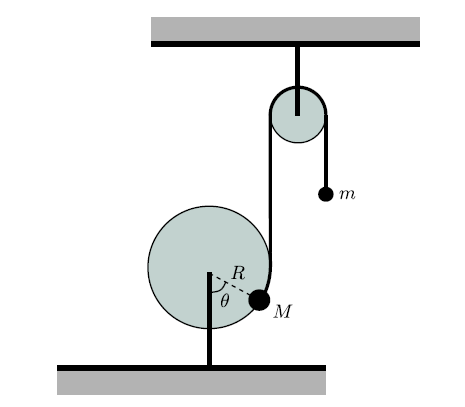
\includegraphics[width=\linewidth]{2014P1Q9.PNG}
\end{figure}
The Lagrangian $\mathcal{L}$ is the difference of the kinetic and potential energies of the system. From the Euler–Lagrange equation find the equation of motion for the angle of rotation of the hoop, $0\leq\theta(t)\leq\pi/2$.\\[5pt]
Derive the equilibrium angle $\theta_0$. Consider small oscillations around $\theta_0$, i.e., let
$\theta(t)=\theta_0+\delta(t)$, where $|\delta|<<\theta_0$. Show that the angular frequency of oscillations is
$$\omega=\bigg(\frac{M-m}{M+m}\bigg)^{1/4}\sqrt{\frac{g}{R}}$$
Comment on the limit $M>> m$.\hfill \textbf{[10]}
\end{enumerate}
\end{qns}
\begin{ans}\leavevmode
\begin{enumerate}[label=(\roman*)]
\item The first order variation of the action $S$ is
$$\delta S=S[q+\delta q]-S[q]=\int_{t_0}^{t_1}\delta q\frac{\partial L}{\partial q}+\frac{\partial L}{\partial\dot{q}}\delta\dot{q}dt=\int_{t_0}^{t_1}\delta q\bigg(\frac{\partial L}{\partial q}-\frac{d}{dt}\frac{\partial L}{\partial\dot{q}}\bigg)dq+\bigg[\frac{\partial L}{\partial\dot{q}}\delta q\bigg]_{t_0}^{t_1}$$
The boundary term is zero since $q$ is fixed at $t_0$ and $t_1$. To find the stationary value of the functional, $\frac{\partial S}{\partial q}=0\implies\frac{\partial L}{\partial q}=\frac{d}{dt}\frac{\partial L}{\partial\dot{q}}$, which is the Euler-Lagrange equation.\\[5pt]
If $L=(q(t),\dot{q}(t))$, then $\frac{\partial L}{\partial t}=0$, and so by the chain rule,
$$\frac{dL}{dt}=\frac{\partial L}{\partial t}+\frac{\partial L}{\partial q}\dot{q}+\frac{\partial L}{\partial \dot{q}}\ddot{q}=0+\frac{d}{dt}\bigg(\frac{\partial L}{\partial\dot{q}}\dot{q}\bigg)$$
which implies $L-\frac{\partial L}{\partial\dot{q}}\dot{q}$ is a constant.
\item The Lagrangian is given to be the difference between kinetic and potential energies
$$\mathcal{L}(\theta,\dot{\theta},t)=\frac{1}{2}(m+M)R^2\dot{\theta}^2-gR[-m\theta+M(1-\cos\theta)]$$
We define the action to be the functional $\mathcal{S}[\theta(t)]=\int\mathcal{L}dt$. We wish to extremize the action, then by the Euler-Lagrange equation in part (i),
$$0=\frac{d}{dt}\frac{\partial\mathcal{L}}{\partial\dot{\theta}}-\frac{\partial\mathcal{L}}{\partial\theta}=\ddot{\theta}(M+m)R^2-gR(-m+M\sin\theta)$$
This gives the equation of motion $$\ddot{\theta}+g\frac{M\sin\theta}{R(m+M)}=\frac{gm}{(M+m)R}$$
Note the first integral of motion (since $\mathcal{L}$ is independent of $t$) gives the conservation of energy.\\[5pt]
At equilibrium, $\ddot{\theta}=0$, and so $\theta_0=\sin^{-1}\frac{m}{M}$. Now perturb $\theta$ about $\theta_0$ with $|\delta(t)|<<\theta_0$, then
$$\ddot{\delta}+\frac{gM}{R(m+M)}\sin(\theta_0+\delta)=\frac{gm}{R(M+m)}=\frac{gM}{R(m+M)}\sin\theta_0$$
Then we have $\ddot{\delta}+\frac{gM\delta}{R(m+M)}\sqrt{1-(m/M)^2}$. This is an equation of simple harmonic motion $\ddot{\delta}=-\omega^2\delta=0$, and hence the angular frequency is 
$$\omega=\sqrt{\frac{gM}{R(M+m)}}\bigg(1-\frac{m^2}{M^2}\bigg)^{1/4}=\sqrt{\frac{g}{R}}\bigg(\frac{M-m}{M+m}\bigg)^{1/4}$$
In the limit $M>>m$, $\omega\approx\sqrt{\frac{g}{R}}$, where $M$ just oscillates about $\theta_0$ without the influence of $m$.
\end{enumerate}
\end{ans}
\newpage
\begin{qns}[Rayleigh-Ritz Method]
The Sturm–Liouville equation is
\begin{equation}
    [-p(x)\psi']'+q(x)\psi=\lambda w(x)\psi\tag{*}
\end{equation}
where $p(x) > 0$ and $w(x) > 0$ for $a\leq x\leq b$, and primes denote differentiation with respect to $x$.
\begin{enumerate}[label=(\roman*)]
\item Show that finding the eigenvalues $\lambda$ is equivalent to finding the stationary values of the functional
$$\Lambda[\psi(x)]=\frac{\int_a^b(p\psi'^2+q\psi^2)dx}{\int_a^b w\psi^2dx}$$
if suitable boundary conditions are satisfied at $x= a$ and $x = b$ (which should be stated).\hfill \textbf{[6]}
\item Let $\lambda_0$ be the lowest eigenvalue and  $\psi_0$ be the associated eigenfunction. A general function $\tilde{\psi}$ can be written as
$$\tilde{\psi}(x)=c_0\psi_0(x)+\sum_{i=1}^\infty c_i\psi_i(x)$$
where $c_0$ and $c_i$ are constants, and  $\psi_i$ ($i$ = 0, 1, 2,...) are orthonormal eigenfunctions of (*) with eigenvalues $\lambda_i\geq\lambda_0$. Show that
$$\tilde{\lambda}=\Lambda[\tilde{\lambda}(x)]=\frac{\lambda_0+\sum_{i=1}^\infty|a_i|^2\lambda_i}{1+\sum_{i=1}^\infty|a_i|^2}$$
where $a_i=\frac{c_i}{c_0}$. Explain how this result allows you to estimate the lowest eigenvalue $\lambda_0$.\hfill \textbf{[6]}
\item Consider the Schrodinger equation
$$-\psi''+x^2\psi=\lambda\psi$$
for $0\leq x<\infty$ and with the boundary conditions $\psi(0) = 0$, $\lim_{x\rightarrow\infty}\psi(x)=0$. Using the trial function $\tilde{\psi}=xe^{-\alpha x}$ with $\alpha$ a real positive constant, estimate the lowest eigenvalue $\lambda_0$.

\hfill \textbf{[8]}
\end{enumerate}
\end{qns}
\newpage
\begin{ans}\leavevmode
\begin{enumerate}[label=(\roman*)]
\item We define the functionals $F[\psi]:=\int_a^bp\psi'^2+q\psi^2dx$ and $G[\psi]:=\int_a^bw\psi^2dx$ such that $\Lambda=\frac{F}{G}$. Its first order variation is 
$$\delta\Lambda=\frac{\delta F+F}{\delta G+G}-\frac{F}{G}=\frac{1}{G}\bigg(\delta F-\frac{F}{G}\delta G\bigg)$$
Then, $0=\frac{\delta\Lambda}{\delta\psi}=\frac{1}{G}[\frac{\delta F}{\delta\psi}-\Lambda\frac{\delta G}{\delta\psi}]$. The value of $\Lambda$ at the stationary point is $\lambda$, and hence to extremize $\Lambda$, it is equivalent to extremizing $F-\lambda G=\int_a^bp\psi'^2+q\psi^2-\lambda w\psi^2dx$. Euler-Lagrange gives us 
$$(2p\psi')'-2q\psi+2\lambda w\psi=0$$
which is the SL equation (*) multiplied by 2. The stationary values of the functional
$$\Lambda=\frac{[p\psi\psi']_a^b+\int_a^b-\psi(p\psi')'+\psi q\psi dx}{\int_a^b\psi w\psi dx}=\frac{[p\psi\psi']_a^b+\langle\psi|\mathcal{L}\psi\rangle}{\langle\psi|\psi\rangle_w}=\lambda$$
if $[p\psi\psi']_a^b=0$ (boundary terms). For this to be true, we choose $\psi(a)=\psi(b)=0$.\item Firstly, we need to show the eigenfunctions $\psi_i$ and $\psi_j$ are orthogonal. $\psi_i$ and $\psi_j$ satisfy $\mathcal{L}\psi_i=\lambda_iw\psi_i$ and $\mathcal{L}\psi_j=\lambda_jw\psi_j$ as long as certain boundary conditions are satisfied. In part (i), we have established $\langle\psi_i|\mathcal{L}\psi_j\rangle=\langle\mathcal{L}\psi_i|\psi_j\rangle$, then the LHS gives $\lambda_j\langle\psi_i|\psi_j\rangle_w$ while the RHS gives $\lambda_i^*\langle\psi_i|\psi_j\rangle_w$. Bringing to one side, we have
$$(\lambda_i^*-\lambda_j)\langle\psi_i|\psi_j\rangle_w=0$$
If $i=j$, since $\langle\psi_i|\psi_i\rangle_w>0$ then $\lambda_i^*=\lambda_i\in\mathbb{R}$, i.e. the eigenvalues are real. If $i\neq j$, $\lambda_i^*=\lambda_i\neq\lambda_j$, then we have $\langle\psi_i|\psi_j\rangle_w=0$, i.e. eigenfunctions corresponding to distinct eigenvalues are orthogonal with respect to the inner product with weight $w$. The eigenfunctions of a SL operator are complete. Assuming the eigenfunctions are also properly normalized, then we can expand a general function $\tilde{\psi}$ in terms of the orthonormal eigenfunctions, i.e. $\tilde{\psi}(x)=\sum_{n=0}^\infty c_n\psi_n$.
$$F[\tilde{\psi}]=\bigg\langle\sum_{p=0}^\infty c_p\psi_p|\mathcal{L}\sum_{n=0}^\infty c_n\psi_n\bigg\rangle=\sum_{p=0}^\infty\sum_{n=0}^\infty c_p^*\lambda_nc_n\langle\psi_p|\psi_n\rangle=\sum_{n=0}^\infty\lambda_n|c_n|^2$$
where $\langle\psi_p|\psi_n\rangle=\delta_{p,n}$. And
$$G{\tilde{\psi}}=\sum_{n=0}^\infty|c_n|^2$$
Hence,
$$\Lambda[\tilde{\psi}]=\frac{\sum_{n=0}^\infty\lambda_n|c_n|^2}{\sum_{n=0}^\infty|c_n|^2}=\frac{\lambda_0+\sum_{n=1}^\infty\lambda_n\frac{|c_n|^2}{|c_0|^2}}{1+\sum_{n=1}^\infty\frac{|c_n|^2}{|c_0|^2}}$$
We thus obtained our desired result with $|a_n|^2=\frac{|c_n|^2}{|c_0|^2}$. One can use this obtained result to estimate the lowest eigenvalue by guessing a trial function that obeys the boundary conditions. Afterwhich, we extremize $\Lambda$ with respect to all the parameters it contains.
\item For the Schrodinger equation, we identify $p(x)=1$, $q(x)=x^2$ and $w(x)=1$. The trial function is $\tilde{\psi}=xe^{-\alpha x}\implies\tilde{\psi}'=e^{-\alpha x}(1-\alpha x)$. The following identity will be helpful: $$I_n(a)=\int_0^\infty x^ne^{-ax}dx=\frac{n!}{a^{n+1}}$$
$$F[\tilde{\psi}]=\int_0^\infty e^{-2\alpha x}(1-2\alpha x+\alpha^2x^2)+x^4e^{-2\alpha x}dx=\frac{1}{2\alpha}-2\alpha\frac{1}{(2\alpha)^2}+\alpha^2\frac{2!}{(2\alpha)^3}+\frac{4!}{(2\alpha)^5}=\frac{1}{4\alpha}+\frac{3}{4\alpha^5}$$
$$G[\tilde{\psi}]=\int_0^\infty x^2e^{-2\alpha x}dx=\frac{2!}{(2\alpha)^3}=\frac{1}{4\alpha^3}$$
$$\Lambda[\tilde{\psi}]=\frac{F[\tilde{\psi}]}{G[\tilde{\psi}}]=4\alpha^3\bigg(\frac{1}{4\alpha}+\frac{3}{4\alpha^5}\bigg)=\alpha^2+\frac{3}{\alpha^2}$$
Then, $0=\frac{\partial\Lambda}{\partial\alpha}=2\alpha-6\alpha^{-3}\implies\alpha=3^{1/4}$. Thus, the lowest eigenvalue is $\lambda_0=\sqrt{3}+\frac{3}{\sqrt{3}}=2\sqrt{3}$.
\end{enumerate}
\end{ans}
\newpage
\subsection{Paper 2}
\begin{qns}[Sturm-Liouville]\leavevmode
\begin{enumerate}[label=(\roman*)]
\item The inner product of two functions $f(x)$ and $g(x)$, defined on the closed interval $[a, b]$, is
$$\langle f|g\rangle=\int_a^bf^*gwdx$$
where $w(x) > 0$. Consider the operator
$$\mathcal{L}=-\frac{1}{w(x)}\bigg[\frac{d}{dx}\bigg(p(x)\frac{d}{dx}\bigg)-q(x)\bigg],\quad a\leq x\leq b$$
where $p(x) > 0$.
\begin{enumerate}[label=(\alph*)]
\item Derive the boundary conditions under which $\mathcal{L}$ is self-adjoint over the range $[a, b]$, with respect to the inner product defined above.\hfill\textbf{[3]}
\item Show that any two eigenfunctions of $\mathcal{L}$ with distinct eigenvalues are orthogonal.\hfill\textbf{[3]}\end{enumerate}
\item Consider the eigenvalue problem
\begin{equation}
    \mathcal{L}y=-x^2y''-xy'-y=\lambda y\tag{*}
\end{equation}
with boundary conditions $y(1) = y(e) = 0$.
\begin{enumerate}[label=(\alph*)]
\item Show that (*) can be written in Sturm–Liouville form and identify the functions $p(x)$, $q(x)$ and $w(x)$.\hfill\textbf{[2]}
\item Find the eigenvalues and orthonormal eigenfunctions of $\mathcal{L}$.\hfill\textbf{[6]}
\item Derive the solution to the inhomogeneous equation $\mathcal{L}y=1$ as an eigenfunction expansion.\hfill\textbf{[6]}
\end{enumerate}
\end{enumerate}
\end{qns}
\begin{ans}\leavevmode
\begin{enumerate}[label=(\roman*)]
\item \begin{enumerate}[label=(\alph*)]
\item For $\mathcal{L}$ to be self-adjoint, we require $\langle y_m|\mathcal{L}y_n\rangle=\langle\mathcal{L}y_m|y_n\rangle$.
\begin{eqnarray}
\langle y_n|\mathcal{L}y_m\rangle&=&-\bigg[\int_a^b y_n^*\frac{d}{dx}\bigg(p(x)\frac{dy_m}{dx}\bigg)-y_n^*q(x)y_m\bigg]dx\nonumber\\&=&-\bigg[-y_n^*p(x)\frac{dy_m}{dx}\bigg]_a^b+\int_a^b \frac{dy_n^*}{dx}p(x)\frac{dy_m}{dx}dx+\int_a^by_n^*q(x)y_mdx\nonumber\\&=&\bigg[y_n^*p(x)\frac{dy_m}{dx}-y_m\frac{dy_n^*}{dx}p(x)\bigg]_a^b-\int_a^b y_m\frac{d}{dx}\bigg(p(x)\frac{dy_n^*}{dx}\bigg)+y_n^*y_mq(x)dx\nonumber
\end{eqnarray}
We require $p>0$ at the boundaries $x=a$, $x=b$, as well as, some combination of Neumann, Dirichlet or Cauchy boundary condition to set the boundary terms zero. 
\item LHS gives $\langle y_j|\lambda_iy_i\rangle$ and RHS gives $\langle\lambda_j^*y_j|y_i\rangle$, then $(\lambda_j^*-\lambda_i)\langle y_j|y_i\rangle=0$. If $i\neq j$ (distinct eigenvalues), then $\lambda_j\neq\lambda_i\implies\langle y_j|y_i\rangle=0$, i.e. orthogonal w.r.t inner product.
\end{enumerate}
\item
\begin{enumerate}[label=(\alph*)]
\item Multiply (*) with an integration factor $\mu$ to cast to Sturm-Liouville form
$$\mathcal{L}y=-\frac{1}{\mu(x)}(\mu(x) x^2y''+\mu(x) xy'+\mu(x)y)=-\frac{1}{\mu}((\mu(x)x^2y')'+\mu(x)y)$$
where we require $\mu'x^2=-\mu x\implies\mu(x)\propto\frac{1}{x}$. Then, we have $\mathcal{L}y=-x((xy')^2+\frac{y}{x})$, such that $w(x)=\frac{1}{x}$, $p(x)=x$ and $q(x)=\frac{1}{x}$.
\item This is an equidimensional differential equation. We substitute $x=e^t$, such that $\frac{d}{dx}\frac{d}{dx}=e^{-2t}(-\frac{d}{dt}+\frac{d^2}{dt^2})$ and $\frac{d}{dx}=e^{-t}\frac{d}{dt}$, thus we get $\mathcal{L}y=-\frac{d^2y}{dt^2}-y$, hence 
$$\frac{d^2y}{dt^2}=-(\lambda+1)y\implies y(x)=A\sin(\sqrt{\lambda+1}\ln x)+B\cos(\sqrt{\lambda+1}\ln x)$$
With the boundary conditions $y(1)=0\implies B=0$ and $y(e)=0\implies\lambda=n^2\pi^2-1$ for $n\in\mathbb{Z}^+$, i.e. discrete eigenvalues. Hence, to find $A$, we need to ensure normalization:
$$1=\langle y|y\rangle_w=\int_1^e|y|^2\frac{1}{x}dx=|A|^2\int_0^1\sin^2(n\pi t)dt=\frac{1}{2}|A|^2\implies y_n(x)=\sqrt{2}\sin(n\pi \ln x)$$
\item Since the eigenfunctions of the Sturm-Liouville operator are complete, write $y=\sum_{n=0}^\infty a_ny_n$ such that $1=\mathcal{L}y=\sum_{n=0}^\infty a_n\lambda_ny_n$. Then,
$$\int_1^ew(x)y_pdx=\sum_{n=0}^\infty a_n\lambda_n\int_1^ey_p^*y_nw(x)dx\implies\int_0^1\sqrt{2}\sin(p\pi t)dt=a_p(p^2\pi^2-1)$$
This gives $a_p=0$ for $p$ even, and $\frac{2\sqrt{2}}{(-1+p^2\pi^2)^{p\pi}}$ for $p$ odd. Hence,
$$y(x)=\frac{4}{\pi}\sum_{n=1}^\infty\frac{1}{(2n-1)((2n-1)^2\pi^2-1}\sin((2n-1)\ln x)$$
\end{enumerate}
\end{enumerate}
\end{ans}
\begin{qns}[Laplace's Equation]\leavevmode
\begin{enumerate}[label=(\roman*)]
\item Let $\Psi(r,\theta)$ be an axisymmetric solution of Laplace’s equation in spherical polar coordinates,
$$\frac{1}{r^2}\frac{\partial}{\partial r}\bigg(r^2\frac{\partial\Psi}{\partial r}\bigg)+\frac{1}{r^2\sin\theta}\frac{\partial}{\partial\theta}\bigg(\sin\theta\frac{\partial\Psi}{\partial\theta}\bigg)=0$$
By the method of separation of variables, derive the general solution
$$\Psi(r,\theta)=\sum_{l=0}^\infty\bigg(a_lr^l+\frac{b_l}{r^{l+1}}\bigg)P_l(\cos\theta)$$
Here, $P_l(\cos\theta)$ is the $l$th Legendre polynomial, i.e., the solution of the differential equation
$$\frac{d}{dx}\bigg((1-x^2)\frac{dP_l}{dx}\bigg)+l(l+1)P_l=0$$
with $x=\cos\theta$, which is regular at $x =\pm 1$.\hfill\textbf{[8]}
\item A surface charge density $\sigma(\theta)=A\sin^2\theta$ lies on the surface of a sphere of radius $R$ centred on the origin. The electrostatic potential $\Psi(r,\theta)$ satisfies Laplace’s equation for $r\neq R$, is continuous and regular everywhere, and tends to zero as $r\rightarrow\infty$. The surface charge causes a discontinuity in the radial gradient of $\Psi$ across $r = R$ given by
$$\lim_{\epsilon\rightarrow0}\bigg(\frac{\partial\Psi}{\partial r}\bigg|_{R+\epsilon}-\frac{\partial\Psi}{\partial r}\bigg|_{R-\epsilon}\bigg)=-\sigma$$
Determine $\Psi$ for $r < R$ and $r > R$.\hfill\textbf{[12]}
\end{enumerate}
[Note: $P_0(x) = 1$ and $P_2(x) = (3x^2 − 1)/2$.]
\end{qns}
\newpage
\begin{ans}\leavevmode
\begin{enumerate}[label=(\roman*)]
\item Use separation of variables: $\Psi(r>R,\theta)=R(r>R)\Theta(\theta)$:
$$\frac{1}{R}\frac{1}{r^2}\frac{d}{dr}\bigg(r^2\frac{dR}{dr}\bigg)=-\frac{1}{r^2\sin\theta}\frac{1}{\Theta}\frac{d}{d\theta}\sin\theta\frac{d\Theta}{d\theta}=\frac{\lambda}{r^2}$$
for some constant $\lambda$. The angular part gives
$$\lambda\Theta=-\frac{1}{\sin\theta}\frac{d\Theta}{d\theta}=-\frac{1}{\sqrt{1-x^2}}(-\sqrt{1-x^2})\frac{d}{dx}\bigg(-(\sqrt{1-x^2})^2\frac{d\Theta}{dx}\bigg)$$
where we substitute $x=\cos\theta$. This result is identical to the hint. At $x=\pm1$, $\Theta(x)=P_l(x)$ with $\lambda=l(l+1)$. The radial part gives
$$\lambda R=\frac{d}{dr}\bigg(r^2\frac{dR}{dr}\bigg)=2rR'+r^2R''$$
Try $R=r^k$, then $k(k+1)=\lambda=l(l+1)\implies k=l,-(l+1)$. Hence, $$R(r)=a_lr^l+b_lr^{-(l+1)}$$ Fitting them together gives the desired $\Psi(r,\theta)$.
$$\Psi(r,\theta)=\sum_{l=0}^\infty\bigg(a_lr^l+\frac{b_l}{r^{l+1}}\bigg)P_l(\cos\theta)$$
\item For $r<R$: $b_l=0$ $\forall l$ since $R(r=0)$ finite. For $r>R$: $a_l=0$ $\forall l$ since $\lim_{r\rightarrow\infty}R(r)=0$. Imposing boundary conditions: $\Psi$ continuous at $r=R$ gives $b_l=a_lR^lR^{l+1}$ $\forall l$, while the discontinuity at $r=R$ for $\frac{\partial\Psi}{\partial r}$ gives
$$-\sum_{l=0}^\infty\bigg(\frac{(l+1)b_l}{R^{l+2}}+a_lR^{l-1}\bigg)P_l(\cos\theta)=-\sigma=-A(1-\cos^2\theta)=\frac{-2A}{3}(P_0+P_2)$$
Comparing coefficients give 
$$\frac{2A}{3}=\frac{b_0}{R^2},\quad\frac{2A}{3}\frac{3b_2}{R^4}+\frac{2a_2}{R},\quad(l+1)\frac{b_l}{R^{l+2}}=-la_lR^{l-1}~\forall l\neq 0,2$$
Solving for the coefficients give $b_0=\frac{2}{3}AR^2$, $b_2=\frac{2}{15}AR^4$, $a_0=\frac{2}{3}AR$, $a_2=\frac{2A}{15R}$ and $a_l=b_l=0$ $\forall l\neq 0,2$.
$$\Psi(r<R,\theta)=\frac{2}{3}ARP_0(\cos\theta)+r^2\frac{2A}{15R}P_2(\cos\theta)=2A\bigg(\frac{R}{3}+\frac{r^2}{15R}(3\cos^2\theta-1)\bigg)$$
$$\Psi(r>R,\theta)=\frac{2AR^2}{3r}P_0(\cos\theta)+\frac{2AR^4}{15r^3}P_2(\cos\theta)=2A\bigg(\frac{R^2}{3r}+\frac{R^4}{15r^3}(3\cos^2\theta-1)\bigg)$$
\end{enumerate}
\end{ans}
\newpage
\begin{qns}[Green's Functions]\leavevmode
\begin{enumerate}[label=(\roman*)]
\item Two scalar functions $\phi(\mathbf{r})$ and $\psi(\mathbf{r})$ are defined in a volume $V$ of three-dimensional space with boundary $S$. Show that
$$\int_V[\phi\nabla^2\psi-\psi\nabla^2\phi]dV=\int_S[\phi\mathbf{\hat{n}}\cdot\boldsymbol{\nabla}\psi-\psi\mathbf{\hat{n}}\cdot\boldsymbol{\nabla}\phi]dS$$
where $\mathbf{\hat{n}}$ is the outward-directed unit normal to $S$.\hfill\textbf{[3]}
\item Suppose that $\phi(\mathbf{r})$ satisfies
$$\nabla^2\phi+k^2\phi=0$$
for some real and positive $k$.
\begin{enumerate}[label=(\alph*)]
\item Introducing the Green’s function $G(\mathbf{r}, \mathbf{r'})$ that satisfies
$$\nabla^2G(\mathbf{r},\mathbf{r'})+k^2G(\mathbf{r},\mathbf{r'})=\delta^{(3)}(\mathbf{r}-\mathbf{r'})$$
show that
$$\phi(\mathbf{r'})=\int_S\phi(\mathbf{r})\mathbf{\hat{n}}\cdot\boldsymbol{\nabla}G(\mathbf{r},\mathbf{r'})dS$$
for $\mathbf{r'}$ in $V$ and a suitable boundary condition for $\mathbf{r}$ on $S$ that you should specify. For the case that $V$ is all space, show that a suitable Green’s function is
$$G(\mathbf{r},\mathbf{r'})=A\frac{e^{ik|\mathbf{r}-\mathbf{r'}|}}{|\mathbf{r}-\mathbf{r'}|}$$
where the constant $A$ should be determined.\hfill\textbf{[10]}
\item Determine the Green’s function for the case that $V$ is the half-space $z\geq0$.\\[5pt]
Assuming that $\phi$ falls to zero sufficiently rapidly as $|\mathbf{r}|\rightarrow\infty$, show that
$$\phi(\mathbf{r'})=-\frac{ik}{2\pi}\int_{z=0}\frac{e^{ikR}}{R}\bigg(1+\frac{i}{kR}\bigg)\cos\theta\phi(\mathbf{r})dS$$
where $R$ is the magnitude of $\mathbf{R}=\mathbf{r'}-\mathbf{r}$, which makes an angle $\theta$ with the positive $z$-direction, and the integral is over the plane $z=0$.\hfill\textbf{[7]}
\end{enumerate}
\end{enumerate}
\end{qns}
\newpage
\begin{ans}\leavevmode
\begin{enumerate}[label=(\roman*)]
\item Invoke Divergence Theorem to $\phi\boldsymbol{\nabla}\psi$ and $\psi\boldsymbol{\nabla}\phi$ separately:
$$\int_{\partial V}\phi\boldsymbol{\nabla}\psi\cdot d\mathbf{S}=\int_V\boldsymbol{\nabla}\cdot(\phi\boldsymbol{\nabla}\psi)dV=\int_V\phi\nabla^2\psi+\boldsymbol{\nabla}\phi\cdot\boldsymbol{\nabla}\psi dV$$
$$\int_{\partial V}\psi\boldsymbol{\nabla}\phi\cdot d\mathbf{S}=\int_V\boldsymbol{\nabla}\cdot(\psi\boldsymbol{\nabla}\phi)dV=\int_V\psi\nabla^2\phi+\boldsymbol{\nabla}\psi\cdot\boldsymbol{\nabla}\phi dV$$
Take the difference :
$$\int_V\phi\nabla^2\psi-\psi\nabla^2\phi dV=\int_{\partial V}(\phi\boldsymbol{\nabla}\psi-\psi\boldsymbol{\nabla}\phi)\cdot d\mathbf{S}$$
\item 
\begin{enumerate}[label=(\alph*)]
\item We set
and $G\rightarrow 0$ on $S$ as $|\mathbf{r}|\rightarrow\infty$. From the result in part (i), let $\psi=G$, then adding $k^2G\psi-k^2\psi G$:
$$\int_V\phi(\nabla^2+k^2)G-G(\nabla^2+k^2)\phi dV=\int_{\partial V}(\phi\boldsymbol{\nabla}G-\psi\boldsymbol{\nabla}G)\cdot d\mathbf{S}$$
where LHS is $\int_V\phi(\mathbf{r})\delta^{(3)}(\mathbf{r}-\mathbf{r'})-0dV$ and RHS is $\int_V(\phi(\mathbf{r})\boldsymbol{\nabla}G-\boldsymbol{0})\cdot d\mathbf{S}$
$$\phi(\mathbf{r'})=\int_S\phi(\mathbf{r})\boldsymbol{\nabla}G(\mathbf{r},\mathbf{r'})\cdot d\mathbf{S}$$
Since the problem has spherical symmetry ($V$ is all space), then $G(\mathbf{r},\mathbf{r'})=G(|\mathbf{r}-\mathbf{r'}|)=G(r)$. We check the suggested solution is indeed a solution:
$$\nabla_{\mathbf{r}}^2G=\frac{1}{r^2}\frac{d}{dr}\bigg(r^2\frac{dG}{dr}\bigg)=\frac{A}{r^2}e^{ikr}\frac{d}{dr}(-1+ikr)=-k^2G$$
To find $A$, we use Divergence Theorem for a sphere of radius $\epsilon$ centred on the origin, $V=\{|\mathbf{r}|=\epsilon\}$.
$$\int_V\nabla^2GdV+k^2\int_VGdV=\int_V\delta(r)dV\implies\lim_{\epsilon\rightarrow0}\frac{dG}{dr}\bigg|_{r=\epsilon}4\pi\epsilon^2=1\implies 1=-\lim_{\epsilon\rightarrow0}Ae^{-k\epsilon}(\epsilon^{-1}+k)4\pi\epsilon$$
Then after taking $\epsilon\rightarrow 0$, we have $A=-\frac{1}{4\pi}$.
\item For $V$ being the half-space, we have a further condition $G(z=0)=0$ and $G\rightarrow 0$ as $|\mathbf{r}|\rightarrow\infty$. By Uniqueness Theorem, we use the method of images. We replace the original problem with one involving images. This is valid as long as the boundary condition is still satisfied and (*) is still satisfied everywhere on $V$ (i.e. add images outside of $V$). Since the solution is unique, this must be the solution to the original problem.\\[5pt]
To preserve the mirror symmetry of the problem (about $z=0$ plane), we place an image of opposing strength at $\mathbf{r'}$ where $\mathbf{r'}$ and $\mathbf{r}$ are related to each other with the $z$-component flipped. Then, the corresponding $G$ of this modified problem satisfies
$$(\nabla^2-k^2)G=\delta^{(3)}(\mathbf{r}-\mathbf{r_0})-\delta^{(3)}(\mathbf{r}-\mathbf{r'})$$
Since the PDE is linear, the solution will be a linear combination of that found earlier:
$$G=\frac{1}{4\pi}\bigg(\frac{e^{ik|\mathbf{r}-\mathbf{r_0}|}}{|\mathbf{r}-\mathbf{r_0}|}-\frac{e^{ik|\mathbf{r}-\mathbf{r'}|}}{|\mathbf{r}-\mathbf{r'}|}\bigg)$$
Then we have
$$\frac{\partial G}{\partial z}\bigg|_{z=0}=\frac{1}{4\pi}\bigg[\bigg(\frac{ike^{ikR}}{R}-\frac{e^{ikR}}{R^2}\bigg)(-\cos\theta)-\bigg(\frac{ike^{ikR}}{R}-\frac{e^{ikR}}{R^2}\bigg)\cos\theta\bigg]=-\frac{e^{ikR\cos\theta}}{2\pi}\bigg(\frac{ik}{R}-\frac{1}{R^2}\bigg)$$
where $R=\sqrt{(x-x')^2+(y-y')^2+z'^2}$. Plugging it back to a previous result, we get our desired result.
$$\phi(\mathbf{r'})=-\int_S\phi(\mathbf{r})\frac{e^{ikR\cos\theta}}{2\pi}\bigg(\frac{ik}{R}-\frac{1}{R^2}\bigg)dS=\frac{-ik}{2\pi}\int_S\phi(\mathbf{r})e^{ikR\cos\theta}\bigg(\frac{1}{R}+\frac{i}{kR^2}\bigg)dS$$
\end{enumerate}
\end{enumerate}
\end{ans}
\newpage
\begin{qns}[Contour Integration]\leavevmode
\begin{enumerate}[label=(\roman*)]
\item 
\begin{enumerate}[label=(\alph*)]
\item For real $a$ and $b$, with $a > b > 0$, show that
$$z^2 + 2i(a/b)z − 1 = 0$$
has a single solution within the unit circle $|z| = 1$ in the complex plane.\hfill\textbf{[4]}
\item By evaluating a suitable contour integral, show that
$$\int_0^{2\pi}\frac{d\theta}{a+b\sin\theta}=\frac{2\pi}{\sqrt{a^2-b^2}}$$
for real $a$ and $b$, with $a > b > 0$.\hfill\textbf{[6]}
\end{enumerate}
\item By integrating the complex function
$$f(z)=\frac{\ln(z+i)}{z^2+1}$$
along the real axis, evaluate the real integral\hfill\textbf{[10]}
$$\int_0^\infty\frac{\ln(x^2+1)}{x^2+1}dx$$
\end{enumerate}
\end{qns}
\begin{ans}\leavevmode
\begin{enumerate}[label=(\roman*)]
\item
\begin{enumerate}[label=(\alph*)]
\item  The solution to the quadratic equation is
$$z_{\pm}=\frac{-2ia/b\pm\sqrt{-4(a^2/b^2)+4}}{2}=-i\frac{a}{b}\pm\sqrt{1-\frac{a^2}{b^2}}=-i\frac{a}{b}\bigg[-1\pm\sqrt{1-(b/a)^2}\bigg]$$
Since $a>b>0$, we must have $|z_+|<1$ and $|z_-|>1$, hence $z_+$ lies inside the unit circle $|z|=1$.
\item Parametrize the contour $\gamma=\{z:~|z|=1\}$ (chosen to be a unit circle) as $z=e^{i\theta}$, then the integral becomes
$$\int_0^{2\pi}\frac{d\theta}{a+b\sin\theta}=\oint_{\gamma}\frac{1}{a+\frac{b}{2i}(z-z^{-1})}\frac{dz}{iz}=\frac{2}{b}\oint_\gamma\frac{1}{-2i\frac{a}{b}z+z^2-1}dz$$
Use residue theorem to evaluate the contour integral:
$$\frac{2}{b}2\pi i\res_{z=z_+}\frac{1}{(z-z_+)(z-z_-)}=\frac{4\pi i}{b(z_+-z_-)}=\frac{2\pi}{\sqrt{a^2-b^2}}$$
\end{enumerate}
\item $f(z)$ has simple pole at $z=i$ and essential branch singularity at $z=-i$. Take the branch cut from $z=-i$ to $-\infty$ along the imaginary axis. Then, close the upper-half plane. 
\begin{center}
    \begin{tikzpicture}
      \draw [->] (-3, 0) -- (3, 0);
      \draw [->] (0, -1) -- (0, 3);

      \draw [black, thick, ->-=0.3, ->-=0.8] (-2, 0) -- (2, 0) node [pos=0.3, below] {$\gamma_0$} arc(0:180:2) node [pos=0.3, right] {$\gamma_R$};

      \node [below] at (-2, 0) {$-R$};
      \node [below] at (2, 0) {$R$};

      \node at (0, 1) {$\times$};
      \node [right] at (0, 1) {$i$};
      \node at (0, -1) {$\times$};
      \node [right] at (0, -1) {$-i$};
      \draw [thick,decorate, decoration=zigzag] (0, -1) -- (0, -3);
    \end{tikzpicture}
  \end{center}
The contour $\gamma=\gamma_R\cup\gamma_0$ encloses the simple pole. Parametrize the contours as $\gamma_0:~z=x$ and $\gamma_R:~z=Re^{i\theta}$. The contour integrals are
$$\int_{\gamma_0}f(z)dz=\int_{-\infty}^\infty\frac{1}{2}\frac{\ln[(x^2+1)e^{i\tan^{-1}(1/x)}]}{2(x^2+1)}dx=\int_0^\infty\frac{\ln(x^2+1)}{x^2+1}dx+\int_{-\infty}^\infty\frac{i\tan^{-1}(1/x)}{2(1+x^2)}dx$$
\begin{align}
\int_{\gamma_R}f(z)dz&=\int_0^\pi\frac{\ln(Re^{i\theta}+i)}{R^2e^{2i\theta}+1}iRe^{i\theta}d\theta\nonumber\\&=\int_0^\pi\ln\bigg[Re^{i\theta}\bigg(1+\frac{ie^{-i\theta}}{R}\bigg)\bigg]\frac{i}{Re^{i\theta}}\bigg(1+R^{-1}e^{-i\theta}\bigg)^{-1}d\theta\nonumber\\&=\int_0^\pi\bigg[\ln(Re^{i\theta})+\frac{ie^{-i\theta}}{R}+O(R^{-2})\bigg]\bigg[\frac{i}{Re^{i\theta}}+O(R^{-2})\bigg]d\theta\nonumber\\&=O(\ln(R)/R)\rightarrow0\nonumber
\end{align}
as $R\rightarrow\infty$. The residue of the enclosed pole is
$$\res_{z=i}f(z)=\lim_{z\rightarrow i}\frac{\ln(z+i)}{z^2+1}(z-i)=\frac{\ln2+i(\pi/2)}{2i}=\frac{\ln 2}{2i}+\frac{\pi}{4}$$
Hence, by residue theorem,
$$2\pi i\res_{z=i}f(z)=\int_{\gamma_0\cup\gamma_R}f(z)dz=\int_{\gamma_0}f(z)dz$$
LHS is $\pi \ln 2+\frac{\pi^2}{2}i$ and RHS is $\int_0^\infty\frac{\ln(x^2+1)dx}{x^2+1}+\int_{-\infty}^\infty\frac{i\tan^{-1}(1/x)}{2(1+x^2)}dx$. Comparing the real parts, we get
$$\int_0^\infty\frac{\ln(x^2+1)dx}{x^2+1}=\pi \ln 2$$
\end{enumerate}
\end{ans}
\begin{qns}[Fourier Transform]
The Fourier transform in $x$ of a function $u(x, t)$ is given by
\begin{equation}
    \tilde{u}(k,t)=\int_{-\infty}^\infty u(x,t)e^{-ikx}dx\tag{*}
\end{equation}
\begin{enumerate}[label=(\roman*)]
\item Consider the following partial differential equation for $u(x, t)$:
\begin{equation}
    \frac{\partial^2u}{\partial t^2}+2\gamma\frac{\partial u}{\partial t}+\gamma^2u=c^2\frac{\partial^2u}{\partial x^2}\tag{**}
\end{equation}
where $\gamma$ and $c$ are real constants. Write down the corresponding ordinary differential equation for $\tilde{u}(k,t)$ defined in (*). You may assume that $u$ and its derivatives vanish
as $|x|\rightarrow\infty$.\hfill\textbf{[2]}
\item Seeking solutions of the form $e^{rt}$ for constant $r$, find the general solution to the Fourier transform of (**) for $\tilde{u}(k, t)$, and hence find the general solution for $u(x, t)$.\hfill\textbf{[8]}
\item Solve (**) for $u(x, t)$ subject to the following initial conditions at $t = 0$:\hfill\textbf{[10]}
$$u=e^{-|x|}\text{ and }\frac{\partial u}{\partial t}=0$$
\end{enumerate}
\end{qns}
\newpage
\begin{ans}\leavevmode
\begin{enumerate}[label=(\roman*)]
\item Assume $u$, $\frac{\partial u}{\partial x}$ and $\frac{\partial u}{\partial t}$ all vanish as $|x|\rightarrow\infty$, then $\mathcal{F}[\frac{\partial^2u}{\partial t^2}]=\frac{\partial^2\tilde{u}}{\partial t^2}$, $\mathcal{F}[\frac{\partial^2u}{\partial x^2}]=-k^2\tilde{u}$ and $\mathcal{F}[\frac{\partial u}{\partial t}]=\frac{\partial\tilde{u}}{\partial t}$. Hence, perform Fourier transform on (**) gives
$$\frac{d^2\tilde{u}}{dt^2}+2\gamma\frac{d\tilde{u}}{dt}+(\gamma^2+(ck)^2)\tilde{u}=0$$
\item Try $\tilde{u}=e^{rt}$, then we have $r=-\gamma\pm ick$. The solution to the Fourier transform of (**) is
$$\tilde{u}(k,t)=A(k)e^{(-\gamma-ick)t}+B(k)e^{(-\gamma+ick)t}$$
Perform inverse Fourier transform,
$$u(x,t)=\frac{e^{-\gamma t}}{2\pi}\int_{-\infty}^\infty[A(k)e^{ik(x-ct)}+B(k)e^{ik(x+ct)}]dk$$
\item Fourier transform the initial conditions
\begin{align}
\tilde{u}(k,0)&=\int_{-\infty}^\infty e^{-|x|}e^{-ikx}dx\nonumber\\&=\int_{-\infty}^0e^{-x(ik-1)}dx+\int_0^\infty e^{-x(ik+1)}dx\nonumber\\&=\frac{1}{1+ik}+\frac{1}{1-ik}\nonumber\\&=\frac{2}{1+k^2}\nonumber
\end{align}
So, $\tilde{u}(k,0)=A(k)+B(k)=\frac{2}{1+k^2}$. Similarly, 
$$A(k)(-\gamma-ick)+(-\gamma+ick)B(k)=\frac{\partial\tilde{u}(k,0)}{\partial t}=0$$
We must have 
$$A(k)=\frac{1}{1+k^2}\bigg(1-\frac{\gamma}{ick}\bigg),\quad B(k)=\frac{1}{1+k^2}\bigg(1+\frac{\gamma}{ick}\bigg)$$
Let $u(x,0)=f(x)=e^{-|x|}$, then the general solution would then be
\begin{align}
u(x,t)&=\frac{e^{-\gamma t}}{2\pi}\int_{-\infty}^\infty\frac{1}{2}\mathcal{F}[f(x)](e^{ik(x-ct)}+e^{ik(x+ct)})+\frac{\gamma}{c}\frac{\mathcal{F}[f(x)]}{2ik}(e^{ik(x+ct)}-e^{ik(x-ct)})dk\nonumber\\&=e^{-\gamma t}\bigg[\frac{1}{2}f(x-ct)+\frac{1}{2}f(x+ct)+\frac{\gamma}{2c}(F(x+ct)-F(x-ct))\bigg]\nonumber
\end{align}
where $\frac{\mathcal{F}[f(x)]}{ik}=\mathcal{F}[F]$ such that $F'=f$, and using inverse Fourier transform:
$$\frac{1}{2\pi}\int_{-\infty}^\infty\mathcal{F}[f(x)]e^{ik(x\pm ct)}dk=f(x\pm ct)=e^{-|x\pm ct|}$$
$$\frac{1}{2\pi}\int_{-\infty}^\infty\frac{\mathcal{F}[f(x)]}{ik}e^{ik(x\pm ct)}dk=F(x\pm ct)$$
The integral of $f(x)=e^{-|x|}$ is
$$F(x)=\frac{|x|}{x}(1-e^{-|x|})$$
One can check by differentiating back, taking note of the two regimes $x>0$ and $x<0$. Also, check 
$$\mathcal{F}[F]=\mathcal{F}[|x|/x]-\mathcal{F}[|x|e^{-|x|}/x]=\frac{2}{ik}-\frac{2ik}{1+k^2}=\frac{2}{ik(1+k^2)}=\frac{1}{ik}\mathcal{F}[f]$$
hence, the general solution is
$$u(x,t)=\frac{e^{-\gamma t}}{2}\bigg[e^{-|x-ct|}+e^{-|x+ct|}+\frac{\gamma}{c}\bigg(\frac{|x+ct|}{x+ct}(1-e^{-|x+ct|})-\frac{|x-ct|}{x-ct}(1-e^{-|x-ct|})\bigg)\bigg]$$
\end{enumerate}
\end{ans}
\newpage
\begin{qns}[Tensors]\leavevmode
\begin{enumerate}[label=(\roman*)]
\item Write down the transformation law for a tensor of order $n$. Use this to define an isotropic tensor.\hfill\textbf{[2]}
\item Consider a three-dimensional vector field with Cartesian components $u_i$. Show that $\frac{\partial u_i}{\partial x_j}$ is an order 2 tensor.\hfill\textbf{[4]}
\item  Write down the transformation law for an axial vector. Under what conditions does an axial vector obey the same transformation law as a vector? Show that the curl of $u_i$ is an axial vector field.\hfill\textbf{[6]}
\item Show that $\frac{\partial u_i}{\partial x_j}$ can be decomposed into the following terms
\begin{equation}
    \frac{\partial u_i}{\partial x_j}=p\delta_{ij}+s_{ij}+\epsilon_{ijk}\omega_k\tag{*}
\end{equation}
where $s_{ij}$ is a symmetric, traceless tensor, $\omega_k$ is an axial vector field, $\epsilon_{ijk}$ is the Levi–Civita symbol, and $\delta_{ij}$ is the Kronecker delta. Find $p$, $s_{ij}$ , and $\omega_k$, expressed in terms of $u_i$.\hfill\textbf{[4]}
\item Consider the three-dimensional vector field
$$u_i=(ax_2,bx_1,0)$$
where $a$ and $b$ are constants. Find $\omega_k$ and the principal values and principal axes of $s_{ij}$ , where $\omega_k$ and $s_{ij}$ are defined in (*).\hfill\textbf{[4]}
\end{enumerate}
\end{qns}
\begin{ans}\leavevmode
\begin{enumerate}[label=(\roman*)]
\item The transformation law for a tensor of order $n$:
$$T'_{i_1i_2...i_n}=(\det L)^pL_{i_1j_1}L_{i_2j_2}...L_{i_nj_n}T_{j_1j_2...j_n}$$
where $p=1$ for pseudotensors and $p=0$ otherwise.\\[5pt]
An isotropic tensor has its components to be the same in all frames, i.e. $T'_{i_1i_2...i_n}=T_{i_1i_2...i_n}$.
\item $\frac{\partial u_i}{\partial x_j}$ transform like $$\bigg(\frac{\partial u_i}{\partial x_j}\bigg)'=\frac{\partial L_{i\alpha}u_\alpha}{\partial x_\beta}L_{j\beta}$$
hence a rank-two tensor.
\item The transformation law for an axial vector is $u_i'=\det L L_{i\alpha}u_\alpha$. When the transformation involves an even number of reflections (recall any rotation can be constructed out of an even number of reflections), then $\det L=1$, so $u_i'=L_{i\alpha}u_\alpha$ and thus transforms like a normal vector.\\[5pt]
The curl of $u_i$ transforms like
$$[\boldsymbol{\nabla}\times\mathbf{u}]_i'=\epsilon_{ijk}\nabla_j'u_k'=\epsilon_{ijk}'L_{j\alpha}L_{k\beta}\nabla_\alpha u_\beta$$
Now how does the Levi-Civita tensor transforms? $\epsilon_{ijk}$ is a pseudotensor and transforms like
$$\epsilon_{ijk}'=\det L\epsilon_{\alpha\beta\gamma}L_{i\alpha}L_{j\beta}L_{k\gamma}$$
Then by the general definition of determinant:
$$\epsilon_{\alpha\beta\gamma}\det L=\epsilon_{ijk}L_{i\alpha}L_{j\beta}L_{k\gamma}$$
Hence,
$$\epsilon_{ijk}'=\det(L)\epsilon_{\alpha\beta\gamma}L_{i\alpha}L_{j\beta}L_{k\gamma}=(\det L)^2\epsilon_{ijk}$$
Since $L$ is orthgoonal, $\det L=\pm1\implies\det(L)^2=1\implies\epsilon_{ijk}'=\epsilon_{ijk}$. Now, we have
$$\epsilon_{\alpha\beta\gamma}\det L L_{i\gamma}=\epsilon_{jks}L_{j\alpha}L_{k\beta}L_{s\gamma}L_{i\gamma}=\epsilon_{jki}L_{j\alpha}L_{k\beta}=\epsilon_{ijk}'L_{j\alpha}L_{k\beta}\implies[\boldsymbol{\nabla}\times\mathbf{u}]_i'=L_{i\gamma}\det L\epsilon_{\alpha\beta\gamma}\nabla_\alpha u_\beta$$
Hence, $\boldsymbol{\nabla}\times\mathbf{u}$ transforms like an axial-vector.
\item We decompose a general rank-two matrix $T$:
$$T_{ij}=S_{ij}-\frac{\Tr(S)}{\Tr(I)}\delta_{ij}+\frac{\Tr(S)}{\Tr(I)}\delta_{ij}+A_{ij}$$
where $S=\frac{1}{2}(T+T^T)$ is a symmetric tensor (further decomposed to extract a traceless tensor and an isotropic tensor) and $A=\frac{1}{2}(T-T^T)$ is an anti-symmetric tensor. But an anti-symmetric rank-two tensor is also equivalent ot an axial-vector, i.e. $A_{ij}=\epsilon_{ijk}\omega_k.$ Then
$$\epsilon_{ijl}A_{ij}=\epsilon_{ijl}\epsilon_{ijk}\omega_k=(\delta_{jj}\delta_{lk}-\delta_{jk}\delta_{lj})\omega_k=(3\delta_{lk}-\delta_{kl})\omega_k=2\delta_{lk}\omega_k\implies\omega_k=\frac{1}{2}\epsilon_{ijk}A_{ij}$$
By inspection, we see that $$s_{ij}=\frac{1}{2}\bigg(\frac{\partial u_i}{\partial x_j}-\frac{\Tr(\boldsymbol{\nabla}\mathbf{u})}{\Tr(I_{2\times 2})}\delta_{ij}\bigg),\quad p=\frac{\Tr(\boldsymbol{\nabla}\mathbf{u})}{\Tr(I_{2\times 2})},\quad \omega_k=\frac{1}{2}\epsilon_{ijk}\frac{1}{2}\bigg(\frac{\partial u_i}{\partial x_j}-\frac{\partial u_j}{\partial x_i}\bigg)$$
\item We have
$$\boldsymbol{\nabla}\mathbf{u}=\begin{pmatrix}0&a&0\\b&0&0\\0&0&0\\\end{pmatrix}\implies\Tr[\boldsymbol{\nabla}\mathbf{u}]=0\implies p=0$$
$$s=\frac{a+b}{2}\begin{pmatrix}0&1&0\\1&0&0\\0&0&0\\\end{pmatrix}$$
$$\boldsymbol{\omega}=\frac{a-b}{2}\begin{pmatrix}0\\0\\1\\\end{pmatrix}$$
The principal values and axes of $s_{ij}$ are the eigenvalues and the eigenvectors respectively.
$$0=\det[s_{ij}-\lambda I]=\det\begin{pmatrix}-\lambda&(a+b)0.5&0\\0.5(a+b)&-\lambda&0\\0&0&-\lambda\\\end{pmatrix}\implies\lambda=0,\pm\frac{1}{2}(a+b)$$
By inspection, the eigenvectors are respectively $(0,0,1)^T$ and $(\pm1,1,0)^T$. Observe that one of the eigenvector is parallel to $\boldsymbol{\omega}$.
\end{enumerate}
\end{ans}
\newpage
\begin{qns}[Normal Modes]
A loaded string, sketched below, consists of a string stretched tightly between two vertical walls with three beads of equal mass $m$, numbered 1, 2, and 3 as shown, attached at regular intervals with spacing $l$. Assume the beads are constrained to move vertically and that the tension in the string, $\tau$ , is positive and constant. Let $z_i$ be the upward displacement of the $i$th bead 
\begin{figure}[H]
    \centering
    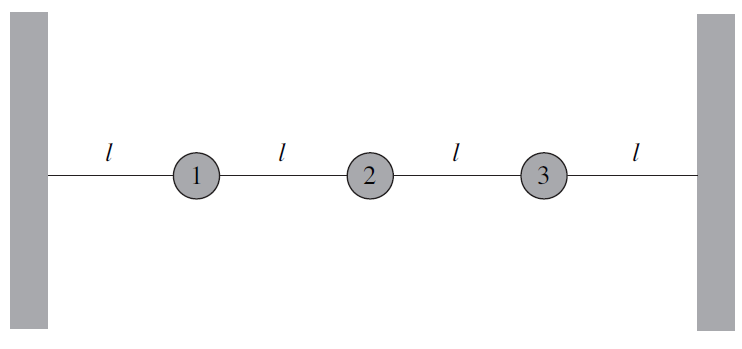
\includegraphics[scale=0.35]{2014P2Q7.PNG}
\end{figure}
\begin{enumerate}[label=(\roman*)]
\item For small displacements, $|z_i|<< l$, the potential energy, $V$ , stored in the string is
$$V=\frac{\tau}{2l}(z_1^2+(z_1-z_2)^2+(z_2-z_3)^2+z_3^2)$$
Find the normal modes of oscillation and their associated frequencies. Sketch the displacements associated with each normal mode.\hfill\textbf{[12]}
\item At time $t = 0$, bead 2 is displaced upwards by a distance $a$, so that $z_2 = a$, while the other beads are at their equilibrium positions ($z_1 = z_3 = 0$), and all beads are initially at rest. Find the subsequent time evolution of the displacement of each bead, and describe the motion in terms of the normal modes.\hfill\textbf{[8]}
\end{enumerate}
\end{qns}
\begin{ans}\leavevmode
\begin{enumerate}[label=(\roman*)]
\item Expressing the potential and kinetic energies in quadratic form:
$$V=\frac{\tau}{2l}\begin{pmatrix}z_1&z_2&z_3\\\end{pmatrix}\begin{pmatrix}2&-1&0\\-1&2&-1\\0&-1&2\\\end{pmatrix}\begin{pmatrix}z_1\\z_2\\z_3\\\end{pmatrix}:=\frac{\tau}{2l}\mathbf{z}^T\mathcal{V}\mathbf{z}$$
$$T=\frac{m}{2}\begin{pmatrix}\dot{z}_1&\dot{z}_2&\dot{z}_3\\\end{pmatrix}\begin{pmatrix}1&0&0\\0&1&0\\0&0&1\\\end{pmatrix}\begin{pmatrix}\dot{z}_1\\\dot{z}_2\\\dot{z}_3\\\end{pmatrix}:=\frac{1}{2}m\mathbf{\dot{z}}\mathcal{T}\mathbf{\dot{z}}$$
The Lagrangian is $\mathcal{L}=T-V$ and is extremized by the Euler-Lagrange equation $\frac{d}{dt}\frac{\partial\mathcal{L}}{\partial\mathbf{\dot{z}}}=\frac{\partial\mathcal{L}}{\partial\mathbf{z}}$, then the equation of motion is $\mathcal{T}\mathbf{\ddot{z}}=-\mathcal{V}\mathbf{z}$, where $T$ is time-independent. We look for solutions of the form $\mathbf{z}(t)=\mathbf{e}e^{i\omega t}$:
\begin{align}
0&=\det(\mathcal{V}-\omega^2\mathcal{T})\nonumber\\&=\det\begin{pmatrix}2(\tau/l)-\omega^2m&-(\tau/l)&0\\-(\tau/l)&2(\tau/l)-\omega^2m&-(\tau/l)\\0&-(\tau/l)&2(\tau/l)-\omega^2m\\\end{pmatrix}\nonumber\\&=(2(\tau/l)u-\omega^2m)(2(\tau/l)^2-4(\tau/l)\omega^2m+m^2\omega^4)\nonumber
\end{align}
The solutions are $\omega_0^2=\frac{2\tau}{ml}$, $\omega_\pm^2=\frac{\tau}{ml}(2\pm\sqrt{2})$ with their corresponding normalized eigenvectors $\mathbf{e_0}=\frac{1}{\sqrt{2m}}(1,0,-1)^T$ and $\mathbf{e_\pm}=\frac{1}{2\sqrt{m}}(1,\mp\sqrt{2},1)^T$. For the mode with frequency $\omega_0$, the centre mass is stationary and the outer masses are in anti-phase (one up, one down). For the mode with frequency $\omega_\pm$, the outer masses are in phase, with the centre mass either in-phase or anti-phase, with a relative amplitude of $\sqrt{2}$.
\item The general solution is
$$\mathbf{z}(t)=\text{Re}[c_0\mathbf{e_0}e^{i\omega_0t}+c_+\mathbf{e_+}e^{i\omega_+t}+c_+\mathbf{e_-}e^{i\omega_-t}]$$
The initial conditions are $\mathbf{z}(0)=(0,a,0)^T$ and $\mathbf{\dot{z}}(0)=\boldsymbol{0}\implies c_0,c_\pm\in\mathbb{R}$. We exploit orthogonality:
$$c_0=\mathbf{e_0}\cdot\mathbf{z}(t=0)=0,\quad c_\pm=\mathbf{e_\pm}\cdot\mathbf{z}(t=0)=\pm a\sqrt{\frac{m}{2}}$$
Hence,
$$\mathbf{z}(t)=\frac{a}{\sqrt{2}}\cos\frac{\tau}{ml}(2-\sqrt{2})t\begin{pmatrix}1\\\sqrt{2}\\1\\\end{pmatrix}-\frac{a}{\sqrt{2}}\cos\frac{\tau}{ml}(2+\sqrt{2})t\begin{pmatrix}1\\-\sqrt{2}\\1\\\end{pmatrix}$$
\end{enumerate}
\end{ans}
\begin{qns}[Group Theory]\leavevmode
\begin{enumerate}[label=(\roman*)]
\item Let $G$ be a finite group. The centre $Z(G)$ of $G$ is the set of elements $z\in G$ that commute with every element $g\in G$, i.e.,
$$Z(G) = \{z \in G| gz = zg, \forall g \in G\}$$
Prove that $Z(G)$ is a subgroup of $G$.\hfill\textbf{[8]}
\item Let $C_n$ be the order $n$ cyclic group.
\begin{enumerate}[label=(\alph*)]
\item Determine whether the product group $C_2 \times C_3$ is isomorphic to the group $C_6$. Do the same for $C_2 \times C_4$ and $C_8$.\hfill\textbf{[8]}
\item What condition do the integers $n$ and $m$ have to satisfy in order for $C_n\times C_m$ to be isomorphic to $C_{n\times m}$?\hfill\textbf{[4]}
\end{enumerate}
\end{enumerate}
\end{qns}
\begin{ans}\leavevmode
\begin{enumerate}[label=(\roman*)]
\item Check subgroup axioms:
\begin{itemize}
    \item Closure: For any $z_1,z_2\in Z$, then $gz_1z_2g^{-1}=gz_1g^{-1}gz_2g^{-1}=z_1z_2\implies z_1z_2\in Z$.
    \item Associativity: Inherited from $G$.
    \item Identity: For $e\in G$, $geg^{-1}=gg^{-1}=e\implies e\in Z$.
    \item Inverse: For any $z\in Z$, $gz^{-1}g^{-1}=(gzg^{-1})^{-1}=z^{-1}\implies z^{-1}\in Z$.
\end{itemize}
\item 
\begin{enumerate}[label=(\alph*)]
\item Let $C_2=\{e,a\}$, $C_3=\{e,b,b^2\}$, then
$$C_2\times C_3=\{(e,e),(e,b),(e,b^2),(a,e),(a,b),(a,b^2)\}$$
where $(e,e)$ is the identity. The generator of $(a,b)$ is
$$\langle(a,b)\rangle=\{(a,b),(e,b^2),(a,e),(e,b),(a,b^2),(a^2,e)\}$$
so $\ord((a,b))=6$ and hence $C_2\times C_3\simeq C_6$. Closure is satisfied. The inverse of $(e,b)$, $(a,e)$ and $(a,b)$ respectively are $(e,b^2)$, $(a,e)$ and $(a,b^2)$. Associativity is inherited from $C_2$ and $C_3$.\\[5pt]
Again, let $C_4=\{e,c,c^2,c^3\}$ and so
$$C_2\times C_4=\{(e,e),(e,c),(e,c^2),(e,c^3),(a,e),(a,c),(a,c^2),(a,c^3)\}$$
Then, $\langle (a,c)\rangle=\{(a,c),(e,c^2),(a,c^3),(e,e)\}$ and so $\ord((a,c))=4$, which happens to be $\lcm(2,4)$. Thus, $C_2\times C_4$ is not isomorphic to $C_8$.
\item For $(a^p,b^q)\in C_n\times C_m$, say $\ord((a^p,b^q))=r$, then 
$$(e,e)=(a^p,b^q)^r=(a^{pr},b^{qr})$$
we require $pr=0$ and $qr=0$ mod $n$ and $m$ respectively. Thus, $r=\lcm(n,m)$.
\end{enumerate}
\end{enumerate}
\end{ans}
\newpage
\begin{qns}[Group Theory]\leavevmode
\begin{enumerate}[label=(\roman*)]
\item State Lagrange’s theorem relating the order of a group to the orders of its subgroups.\hfill\textbf{[2]}
\item The symmetry group $D_N$ of a regular $N$-sided polygon is generated by elements $R$ and $m$, with $R^N= I$, $m^2 = I$ and $Rm = mR^{−1}$.
\begin{enumerate}[label=(\alph*)]
\item List the distinct group elements of $D_5$ and indicate the geometric action of all order 2 elements on a sketch.\hfill\textbf{[5]}
\item Find all proper subgroups of $D_5$.\hfill\textbf{[4]}
\item Explain the notion of a conjugacy class of a finite group and determine the conjugacy classes of $D_5$. Determine which of the proper subgroups of $D_5$ are normal.\hfill\textbf{[9]}
\end{enumerate}
\end{enumerate}
\end{qns}
\begin{ans}\leavevmode
\begin{enumerate}[label=(\roman*)]
\item Lagrange's theorem states that for $H\leq G$, $\frac{|G|}{|H|}\in\mathbb{N}$.
\begin{enumerate}[label=(\alph*)]
\item The group $D_5$ is
$$D_5=\{I,R,R^2,R^3,R^4,m,mR,mR^2,mR^3,mR^4\}$$
The order 2 groups are $\{I,m\}$, $\{I,mR\}$, $\{I,mR^2\}$, $\{I,mR^3\}$ and $\{I,mR^4\}$ since $(mR^n)^2=\Id$ $\forall n\in\mathbb{N}$. The generator $\langle m\rangle$ flips the pentagon about an axis passing through the centre, while the generators $\langle mR^n\rangle$ flips the pentagon followed by a rotation of $\frac{n2\pi}{5}$ radians about the centre, in the plane of the pentagon.
\item The proper subgroups of $D_5$ are
$$\{I,m\},\quad\{I,mR\},\quad\{I,mR^2\},\quad\{I,mR^3\},\quad\{I,mR^4\}$$
\item The conjugacy class of $h\in G$ (written as $\ccl(h)$) is
$$\ccl(h):=\{k\in G\text{ such that }k=ghg^{-1}\text{ for some }g\in G\}$$
$g*h=ghg^{-1}$ is said to be the conjugate action. If $g_i$ is conjugate to $g_j$, write $g_i\sim g_j$, where $hg_ih^{-1}=g_j$ for some $h\in G$. This action is transitive, i.e. $g_1\sim g_2,g_2\sim g_3\implies g_1\sim g_3$:
$$h_1g_1h_1^{-1}=g_2=h_2g_3h_2^{-1}=(h_2^{-1}h_1)g_1(h_2^{-1}h_1)^{-1}=g_3\implies g_1\sim g_3$$
Furthermore, if two elements are conjugate to each other, they must be of the same order. Let $|g_1|=p$, $|g_2|=q$, then
$$e=g_2^q=(h_1g_1h_1^{-1})^q=h_1g_1^qh_1^{-1}\implies h_1^{-1}eh_1=g_1^q\implies e=g_1^q$$
Hence, $q=np$ for $n\in\mathbb{Z}^+$. Similarly, $p=mq$ for $m\in\mathbb{Z}^+$. Hence, $p=q$.\\[5pt]
Lastly, any element that commutes with all other elements is in a conjugacy class of its own.
$$g_ihg_i^{-1}=hg_ig_i^{-1}=he=h~\forall i$$
The conjugacy classes of $D_5$ are
$$\{I\},\quad\{R,R^4\},\quad\{R^2,R^3\},\{m,mR,mR^2,mR^3,mR^4\}$$
A normal subgroup $H$ has the property that it's left and right cosets are the same, i.e. $g_iH=Hg_i$ $\forall g_i$, so $g_iHg_i^{-1}=H$, which means that $H$ is built out of the union of complete conjugacy classes. In general, it can be shown that if $H\leq G$ such that $|H|=\frac{1}{2}|G|$, then $H\lhd G$, so
$$\{I,R,R^2,R^3,R^4\}$$
is a normal subgroup of $D_5$. This is the only proper normal subgroup.
\end{enumerate}
\end{enumerate}
\end{ans}
\newpage
\begin{qns}[Representation Theory]\leavevmode
\begin{enumerate}[label=(\roman*)]
\item Explain what is meant by a representation $D$ of a group $G$. Define the terms faithful representation, equivalent representation, and the character of a representation.\hfill\textbf{[4]}
\item Construct the group table for the order 4 cyclic group $C_4=\{I,a,a^2,a^3\}$.\hfill\textbf{[4]}
\item Consider the following faithful representations of $C_4$:
$$D_1=\begin{pmatrix}1&0\\0&1\\\end{pmatrix},\quad D_2=\begin{pmatrix}0&1\\-1&0\\\end{pmatrix},\quad D_3=\begin{pmatrix}-1&0\\0&-1\\\end{pmatrix},\quad D_4=\begin{pmatrix}0&-1\\1&0\\\end{pmatrix}$$
and
$$E_1 =\begin{pmatrix}1&0\\0&1\\\end{pmatrix},\quad E_2 =\begin{pmatrix}i&0\\0&i\\\end{pmatrix},\quad E_3 =\begin{pmatrix}-1&0\\0&-1\\\end{pmatrix},\quad E_4 =\begin{pmatrix}-i&0\\0&-i\\\end{pmatrix}$$
Determine whether the representations $D$ and $E$ are equivalent or inequivalent, clearly justifying your answer. Find the characters of each representation.\hfill\textbf{[4]}
\item Consider a three-dimensional representation, $T$, of $C_4$ for which the element $a$ is represented by
$$T(a)=\begin{pmatrix}1&0&0\\0&0&b\\0&c&0\\\end{pmatrix}$$
What are the conditions on the real constants $b$ and $c$ such that $T$ is: (1) a faithful representation; and (2) an unfaithful representation of $C_4$?\hfill\textbf{[8]}
\end{enumerate}
\end{qns}
\begin{ans}\leavevmode
\begin{enumerate}[label=(\roman*)]
\item A representation $D$ of a group $G$ is a homomorphism between elements of the group and a set of invertible matrices. The definitions are:
\begin{itemize}
\item A faithful representation is an injective homomorphism, i.e. the identity matrix only has one pre-image (trivial kernel). 
\item Two representations $D$ and $D'$ are equivalent if $\exists$ a similarity transformation $S$ such that $D'(g_i)=SD(g_i)S^{-1}$ $\forall i$.
\item The character of a representation is the vector of the traces of the matrices used to represent the elements.
\end{itemize}
\item The group table of $C_4$ is
$$\vbox{\tabskip0.5em\offinterlineskip
    \halign{\strut$#$\hfil\ \tabskip1em\vrule&&$#$\hfil\cr
       & I & a &a^2&a^3 \cr
    \noalign{\hrule}\vrule height 12pt width 0pt
    I & I & a &a^2&a^3 \cr
    a & a & a^2 & a^3 & I \cr
    a^2 & a^2 &a^3 & I &a \cr
    a^3 & a^3 & I & a& a^2\cr
}}$$
\item Equivalent representations must have the same characters as the trace is invariant under cyclic permutations: $\forall g_i$, we have
$$\Tr(D'(g_i))=\Tr(SD(g_i)S^{-1})=\Tr(S^{-1}SD(g_i))=\Tr(D(g_i))$$
Since $\Tr(E_2),\Tr(E_4)\in\mathbb{C}$, while $\Tr(D_i)\in\mathbb{R}$ $\forall i$, then no similarity transformation can be found. The characters are $\chi_D=\{2,0,-2,0\}$ and $\chi_E=\{2,-2,2i,-2i\}$.
\item Since $T$ is a representation, it must be a homomorphic mapping. We have
$$T(a)=\begin{pmatrix}1&0&0\\0&0&b\\0&c&0\\\end{pmatrix},~ T(a)^2=\begin{pmatrix}1&0&0\\0&bc&0\\0&0&bc\\\end{pmatrix},~ T(a)^3=\begin{pmatrix}1&0&0\\0&0&b^2c\\0&bc^2&0\\\end{pmatrix},~ T(a)^4=\begin{pmatrix}1&0&0\\0&b^2c^2&0\\0&0&b^2c^2\\\end{pmatrix}$$
We require $T(I)=T(a^4)=T(a)^4$, so $b^2c^2=1$. We either have $bc=-1$ (then $T(a)$, $T(a)^2=T(a^2)$, $T(a)^3=T(a^3)$ and $T(a)^4=T(a^4)$ are distinct matrices, hence faithful representation) or $bc=+1$ (unfaithful representation with kernel $\{I,a^2\}$ since $T(a^2)=T(a)^2=I$).
\end{enumerate}
\end{ans}
\newpage
\section{2015}
\subsection{Paper 1}
\begin{qns}[Vector Calculus]
Consider a toroidal body defined parametrically in the Cartesian coordinate system $x = (x, y, z)$ as the region satisfying
\begin{eqnarray}
x &=& (1 + r\sin\alpha) \cos\beta\nonumber\\
y&=&(1 + r\sin \alpha) \sin\beta ,\nonumber\\
z&=&r\cos\alpha\nonumber
\end{eqnarray}
with $0\leq r\leq R$, $−\pi\leq\alpha<\pi$ and $0\leq\beta<2\pi$ for constant $0 < R < 1$.
\begin{enumerate}[label=(\alph*)]
    \item For a toroidal coordinate system $(r, \alpha, \beta)$, determine the Cartesian components of the vectors $\mathbf{h_r}$, $\mathbf{h_\alpha}$, $\mathbf{h_\beta}$ such that the Cartesian differential $d\mathbf{x}$ is given by
$$d\mathbf{x} = \mathbf{h_r}dr +\mathbf{h_\alpha}d\alpha + \mathbf{h_\beta}d\beta,$$
and hence establish whether or not the toroidal coordinate system is orthogonal. Determine the Jacobian for the coordinate transformation.\hfill \textbf{[8]}
\item Suppose the toroidal body is immersed in a vector field $\mathbf{F}(\mathbf{x})=\boldsymbol{\nabla}\Omega+\boldsymbol{\nabla}\times\mathbf{U}$, where $\Omega$ is a scalar field and $\mathbf{U}$ is a vector field. Consider the integral
$$I=\int_S\mathbf{F}\cdot d\mathbf{S},$$
where $S$ is the surface of the body and $d\mathbf{S}$ is an element of vector area. Why does $I$ not depend on $\mathbf{U}$?\hfill \textbf{[3]}
\item Determine $I$ for the case $\Omega=z^4-xyz+e^{-3y}\cos(3x)+e^{2x}\sin(2y)$.\hfill \textbf{[9]}
\end{enumerate}
\end{qns}
\begin{ans}\leavevmode
\begin{enumerate}[label=(\alph*)]
    \item We have
$$\mathbf{h_r}=\begin{pmatrix}\sin\alpha\cos\beta\\\sin\alpha\sin\beta\\\cos\alpha\\\end{pmatrix};\quad\boldsymbol{h_\alpha}=\begin{pmatrix}r\cos\alpha\cos\beta\\r\cos\alpha\sin\beta\\-r\sin\alpha\\\end{pmatrix};\quad\boldsymbol{h_\beta}=\begin{pmatrix}-(1+r\sin\alpha)\sin\beta\\(1+r\sin\alpha)\cos\beta\\0\\\end{pmatrix}$$
One can show that they are mutually orthogonal, i.e. $\boldsymbol{h_r}\cdot\boldsymbol{h_\alpha}=\boldsymbol{h_\beta}\cdot\boldsymbol{h_\alpha}=\boldsymbol{h_r}\cdot\boldsymbol{h_\beta}=0$, hence the toroidal coordinate system is orthogonal. The Jacobian will simply be
$$J=\begin{vmatrix}\sin\alpha\cos\beta&r\cos\alpha\cos\beta&-(1+r\sin\alpha)\sin\beta\\\sin\alpha\sin\beta&r\cos\alpha\sin\beta&(1+r\sin\alpha)\cos\beta\\\cos\alpha&-r\sin\alpha&0\\\end{vmatrix}=r(1+r\sin\alpha)$$
which is zero only for $r=0$ as $0\leq r\leq R<1$.
\item The toroidal body has a closed surface (no boundary), so the closed loop integral is zero, so the integral is 
$$I=\int_S(\boldsymbol{\nabla}\Omega+\boldsymbol{\nabla}\times\mathbf{U})\cdot d\mathbf{S}=\int_S\boldsymbol{\nabla}\Omega\cdot d\mathbf{S}+\int_{\partial S}\mathbf{U}\cdot d\mathbf{l}=\int_S\boldsymbol{\nabla}\Omega\cdot d\mathbf{S}$$
\item We evaluate $I$ by using divergence theorem.
$$I=\int_S\boldsymbol{\nabla}\Omega\cdot d\mathbf{S}=\int_V\boldsymbol{\nabla}\cdot\boldsymbol{\nabla}\Omega dV=\int_V\begin{pmatrix}\partial_x\\\partial_y\\\partial_z\\\end{pmatrix}\cdot\begin{pmatrix}-yz-3e^{-3y}\sin(3x)+2e^{2x}\sin(2y)\\-xz-3e^{-3y}\cos(3x)+2e^{2x}\cos(2y)\\4z^3-xy\\\end{pmatrix}dV$$
$$=\int_0^R\int_{-\pi}^\pi \int_0^{2\pi}12r^2\cos^2\alpha r(1+r\sin\alpha)d\beta d\alpha dr=6\pi^2R^4$$
where $\int_{-\pi}^\pi\cos^2\alpha\sin\alpha d\alpha=0$ and $\int_{-\pi}^\pi\cos^2\alpha d\alpha=\pi$.
\end{enumerate}
\end{ans}
\newpage
\begin{qns}[Partial Differential Equation]
In two spatial dimensions the time evolution of a scalar field $u(x, y, t)$ is given by
\begin{equation}
\frac{\partial u}{\partial t}=\nabla^2u+\beta\frac{\partial u}{\partial x}\tag{*}
\end{equation}
for constant $\beta$.
\begin{enumerate}[label=(\alph*)]
    \item Consider the domain $0\leq x\leq 1$, $0\leq y\leq 1$ with boundary conditions $\frac{\partial u}{\partial y}=0$ on $y = 0$ and $u = 0$ on the other three boundaries. Use separation of variables to determine the general solution of (*) satisfying the boundary conditions and show that at $t = 0$ this reduces to
$$u(x,y,0)=\sum_{m=1}^\infty\sum_{n=1}^\infty A_{mn}e^{-\frac{\beta}{2}x}
\sin(m\pi x)\cos\bigg(\frac{2n-1}{2}\pi y\bigg),$$ 
for some set of constants $A_{mn}$.\hfill \textbf{[14]}
\item Determine the constants $A_{mn}$ required for $u$ to satisfy the initial condition\hfill \textbf{[6]}
$$u(x,y,0)=x(1-x)e^{-\frac{\beta}{2}x}\cos\frac{3}{2}\pi y$$
\end{enumerate}
\end{qns}
\begin{ans}\leavevmode
\begin{enumerate}[label=(\alph*)]
    \item Since the boundary conditions are homogeneous, we use separation of variables, $u(x,y,t)=X(x)T(t)Y(y)$. Then,
$$\frac{T'}{T}=\frac{X''}{X}+\beta\frac{X'}{X}+\frac{Y''}{Y}$$
the boundary conditions suggest the form $Y\sim\cos y$. So, let
$$\frac{T'}{T}=-\mu;\quad \frac{X''}{X}+\beta\frac{X'}{X}=-\lambda;\quad \frac{Y''}{Y}=-\mu+\lambda$$
We thus obtain a 2nd order differential equation for $X$, i.e. $X''+\beta X'+\lambda X=0$ such that we get
$$X(x)=Pe^{-\beta/2x}\sin(\sqrt{4\lambda-\beta^2}x)$$
where $\beta^2-4\lambda<0$. Similarly, we have $Y=Q\cos(\sqrt{\mu-\lambda}y)$ and $T=Re^{-\mu t}$, where $P$, $Q$ and $R$ are constants. The general solution is thus
$$u(x,y,t)=Ce^{-\beta x/2}\sin(\sqrt{4\lambda-\beta^2}x)\cos(\sqrt{\mu-\lambda}y)e^{-\mu t}$$
We thus impose the boundary conditions. $u(0,y,t)=0\implies\sqrt{4\lambda-\beta^2}=m\pi$ where $m\in\mathbb{Z}$; $u(x,1,t)=0\implies\sqrt{\mu-\lambda}=\frac{2n-1}{2}\pi$ for $n\in\mathbb{Z}$. Hence, $$\mu=\lambda+\frac{(2n-1)^2}{2^2}\pi^2=\frac{m^2\pi^2+\beta^2}{4}+\frac{(2n-1))^2}{2^2}\pi^2$$ By relabelling the constant as $A_{mn}$ and trivially set $t=0\implies e^{-\mu t}=1$, we get the desired form for $u(x,y,t)$.
\item Let $f(x)=x(1-x)$, then using Fourier series,
\begin{eqnarray}
f(x)e^{-\beta x/2}\cos(1.5\pi y)&=&\sum_{n=1}^\infty\sum_{m=1}^\infty A_{mn}\cos\bigg(\frac{2n-1}{2}\pi y\bigg)\sin(m\pi x)e^{-\beta x/2}\nonumber\\
f(x)\int_0^1\cos(1.5\pi q-y)\cos\bigg(\frac{2p-1}{2}\pi y\bigg)dy&=&\int_0^1\sum_{n=1}^\infty\sum_{m=1}^\infty A_{mn}\cos\bigg(\frac{2n-1}{2}\pi y\bigg)\cos\bigg(\frac{2p-1}{2}\pi y\bigg)dy\sin(m\pi x)\nonumber\\
\int_0^1x(1-x)\frac{1}{2}\delta_{2,p}\sin(\gamma\pi x)dx&=&\frac{1}{2}\int_0^1\sum_{m=1}^\infty A_{m2}\sin(\gamma \pi x)\sin(m\pi x)dx\nonumber\\\implies A_{k,2}&=&\frac{8}{(2k+1)^3\pi^2}\nonumber
\end{eqnarray}
where $2k+1=\gamma$.
\end{enumerate}
\end{ans}
\newpage
\begin{qns}[Green's Functions]\leavevmode
\begin{enumerate}[label=(\alph*)]
    \item Use the method of Green’s functions to solve
$$\frac{d^2y}{dx^2}-y=f(x)$$
for $0\leq x\leq 1$, with the boundary conditions $y(0) = y(1) = 0$.\hfill \textbf{[9]}\\[5pt]
[You may use the identity $\sinh a \cosh b − \cosh a \sinh b = \sinh(a − b)$.]
\item A forced damped harmonic oscillator satisfies the equation
$$\frac{d^2x}{dt^2}+2\frac{dx}{dt}+(1+\mu^2)x=g(t),$$
where $\mu$ is a positive constant.
\begin{enumerate}[label=(\roman*)]
    \item Solve this equation for $t\geq0$ with initial conditions $x=\frac{dx}{dt}=0$ at $t=0$.\hfill \textbf{[7]}
    \item Assume that $|g(t)|<Ce^{-at}$ where $C$ and $a$ are constants with $a > 0$. Prove that $x(t)\rightarrow0$ as $t\rightarrow\infty$. \hfill \textbf{[4]}
\end{enumerate}
\end{enumerate}
\end{qns}
\begin{ans}\leavevmode
\begin{enumerate}[label=(\alph*)]
    \item The homogeneous ODE has the solution $y_a=\cosh(x)$ and $y_b=\sinh(x)$. The corresponding Green's function satisfy $$\frac{\partial^2G}{\partial x^2}-G=\delta(x-\xi),\quad G(0,\xi)=G(1,\xi)=0$$
    Integrate around an infinitesimal region around $x=\xi$, we obtain the jump condition $[G']_{\xi^-}^{\xi^+}=1$. $G$ is continuous everywhere including $x=\xi$ (otherwise, $G''\propto\delta'(x-\xi)$, which is a contradiction). Using the homogeneous solutions and the boundary conditions, 
    $$G(x,\xi)=
\left\{
        \begin{array}{ll}
      A\sinh(x) & 0\leq x<\xi\leq 1\\
      C\sinh(x-1) &0\leq\xi< x\leq 1
        \end{array}
    \right.$$
At $x=\xi$, the continuity condition and jump condition give respectively 
$$A\sinh\xi=C\sinh(\xi-1)$$
$$-A\cosh\xi+C\cosh(\xi-1)=1$$ 
$$\begin{pmatrix}C\\A\\\end{pmatrix}=\frac{1}{\cosh(\xi-1)\sinh\xi+\cosh\xi\sinh(\xi-1)}\begin{pmatrix}\sinh\xi&\cosh\xi\\\sinh(\xi-1)&\cosh(\xi-1)\\\end{pmatrix}\begin{pmatrix}1\\0\\\end{pmatrix}=\frac{1}{\sinh(1)}\begin{pmatrix}\sinh(\xi)\\\sinh(\xi-1)\\\end{pmatrix}$$
    $$\implies G(x,\xi)=
\left\{
        \begin{array}{ll}
      \sinh(x)\frac{\sinh(\xi-1)}{\sinh(1)} & 0\leq x<\xi\leq 1\\
      \frac{\sinh\xi}{\sinh(1)}\sinh(x-1) &0\leq\xi< x\leq 1
        \end{array}
    \right.$$
The general solution will thus be $$y(x)=\int_0^1G(x,\xi)f(\xi)d\xi=\frac{\sinh(x)}{\sinh(1)}\int_x^1f(\xi)\sinh(\xi-1)d\xi+\frac{\sinh(x-1)}{\sinh(1)}\int_0^xf(\xi)\sinh(\xi)d\xi$$
\item \begin{enumerate}[label=(\roman*)]
    \item For the homogeneous second order ODE, we try the ansatz $x=e^{\lambda t}$, then we obtain the characteristic equation $\lambda^2+2\lambda+(1+\mu^2)=0$ which has solutions $\lambda=-1\pm i\mu$, hence the homogeneous solutions are $x=e^{-t}e^{\pm i\mu t}$. Then, our corresponding Green's function will be
        $$ G(t,\tau)=
\left\{
        \begin{array}{ll}
      Ae^{-t}\sin(\mu t+\phi) & 0\leq t<\tau<\infty\\
      Be^{-t}\sin(\mu t+\theta) &0\leq\tau< t<\infty
        \end{array}
    \right.$$
    where $\theta$, $\phi$, $A$ and $B$ are constants to be found. This Green's function satisfy
    $$\frac{\partial^2G(t,\tau)}{\partial t^2}+2\frac{\partial G(t,\tau)}{\partial t}+(1+\mu^2)G(t,\tau)=\delta(t-\tau),\quad G(0,\tau)=G'(0,\tau)=0$$
    Integrate this around an infinitesimal region around $t=\tau$ again, we obtain the jump condition at $t=\tau$ to be $[G']_{\tau^-}^{\tau^+}=1$. Similarly, $G$ is continuous $\forall t$. At $t=\tau$, the continuity and jump condition give respectively $$0=Be^{-\tau}\sin(\mu\tau+\theta)\implies\mu\tau=-\theta$$
    $$B e^{-\tau} e^{-(\tau-\tau)}(\mu\cos(\mu(\tau-\tau))-\sin(\mu(\tau-\tau)))=1\implies Be^{-\tau}\mu=1$$
    Hence, 
     $$ G(t,\tau)=
\left\{
        \begin{array}{ll}
      0 & 0\leq t<\tau<\infty\\
      \frac{1}{\mu}e^{-(t-\tau)}\sin(\mu(t-\tau)) &0\leq\tau< t<\infty
        \end{array}
    \right.$$
    The general solution is thus
$$x(t)=\int_0^t\frac{1}{\mu}e^{-(t-\tau)}\sin(\mu(t-\tau))g(\tau)d\tau$$
\item We have $|g(t)|<Ce^{-at}$, and so 
\begin{eqnarray}
|x(t)|&\leq&\int_0^t\frac{C}{\mu}e^{-(t-\tau)}\sin(\mu(t-\tau))e^{-a\tau}d\tau\nonumber\\&\leq&\frac{C}{\mu}e^{-t}\text{Im}\bigg[\int_0^te^{\tau(1-a)+i\mu(t-\tau)}d\tau\bigg]\nonumber\\&=&\frac{C}{\mu}e^{-t}\text{Im}\bigg[e^{i\mu\tau}\bigg[\frac{e^{\tau(1-a-i\mu)}}{1-a+i\mu}\bigg]_0^t\bigg]\nonumber
\end{eqnarray}
which approaches zero as $t\rightarrow\infty$.
\end{enumerate}
\end{enumerate}
\end{ans}
\newpage
\begin{qns}[Fourier Transform]
A radio station wishes to analyse its broadcast of the signal $a(t)$ using Fourier analysis. As a test signal, the radio station chooses a single pulse given by
$$a(t)=
\left\{
        \begin{array}{ll}
      1 & |t|<1 \\
      0 & \text{otherwise}
        \end{array}
    \right.$$
\begin{enumerate}[label=(\alph*)]
\item Determine $\tilde{a}(\omega)$, the Fourier transform of $a(t)$.\hfill \textbf{[3]}
\item Due to bandwidth limitations, the radio station decides to filter the signal so that it broadcasts
$$b(t)=\int_{-\infty}^\infty a(s)f(t-s)ds,$$
where the filter $f(t)$ is defined as
$$f(t)=
\left\{
        \begin{array}{ll}
      1-|t| & |t|<1 \\
      0 & \text{ otherwise}
        \end{array}
    \right.$$
Determine $\tilde{f}(\omega)$, the Fourier transform of $f(t)$, and hence use the convolution theorem to derive an expression for $\tilde{b}(\omega)$, the Fourier transform of $b(t)$.\hfill \textbf{[7]}
\item Due to reflections from a mountain range, the signal received by the listeners can be modelled by
$$r(t)=b(t)+\alpha b(t-\tau),$$
where $\alpha$ is the relative strength of the reflected signal and $\tau$ is the delay in receiving the reflection. Determine $\tilde{r}(\omega)$, the Fourier transform of $r(t)$.\hfill \textbf{[4]}
\item Measurements of the received signal suggest it is well approximated by $s(t)$ with Fourier transform
$$\tilde{s}(\omega)=2(1+\epsilon\omega^2)e^{-\omega^2/4}$$
for some constant $\epsilon$. Determine $s(t)$.\hfill \textbf{[6]}
\end{enumerate}
[You may assume $\int_{-\infty}^\infty e^{-(z-ia)^2}dz=\sqrt{\pi}$ for real $a$.]
\end{qns}
\begin{ans}\leavevmode
\begin{enumerate}[label=(\alph*)]
\item The Fourier transform of $a(t)$ is
$$\tilde{a}(\omega)=\frac{1}{\sqrt{2\pi}}\int_{-1}^1e^{-i\omega t}dt=\sqrt{\frac{2}{\pi}}\sinc(\omega)$$
\item The Fourier transform of $f(t)$ is
$$\tilde{f}(\omega)=\frac{1}{\sqrt{2\pi}}\int_{-1}^1(1-|t|)e^{-i\omega t}dt=\frac{1}{\sqrt{2\pi}}\int_{-1}^1(1-|t|)\cos(\omega t)dt=\frac{2}{\sqrt{2\pi}}\int_0^1(1-t)\cos\omega tdt=\sqrt{\frac{2}{\pi}}\frac{2\sin^2(\omega/2)}{\omega^2}$$
By the Convolution Theorem, if $b(t)=a(t)*f(t)$, then $$\tilde{b}(\omega)=\tilde{a}(\omega)\tilde{f}(\omega)\sqrt{2\pi}=\sqrt{\frac{2}{\pi}}\frac{4}{\omega^3}\sin(\omega)\sin^2(\omega/2)$$
\item The Fourier transform of $r(t)$ is
$$\tilde{r}(\omega)=\tilde{b}(\omega)+\alpha\int_{-\infty}^\infty b(t-\tau)e^{-i\omega t}d\omega\frac{1}{\sqrt{2\pi}}=\tilde{b}(\omega)+\alpha\int_{-\infty}^\infty b(s)e^{-i\omega (s+\tau)}ds\frac{1}{\sqrt{2\pi}}=\tilde{b}+\alpha\tilde{b}e^{-i\omega\tau}$$
\item The inverse Fourier transform of $s$ is
$$s(t)=\frac{1}{\sqrt{2\pi}}\int_{-\infty}^\infty\tilde{s}(\omega)e^{i\omega t}d\omega=\frac{1}{\sqrt{2\pi}}\int_{-\infty}^\infty 2(1+\epsilon\omega^2)e^{-\omega^2/4}e^{i\omega t}d\omega=\sqrt{\frac{2}{\pi}}\int_{-\infty}^\infty(1+\epsilon\omega^2)e^{-(\omega-2it)^2/4}e^{-t^2}d\omega$$
$$\implies=\sqrt{\frac{2}{\pi}}e^{-t^2}\bigg[(1-4\epsilon t^2)\int_{-\infty}^\infty e^{-\omega'^2/4}d\omega'+\epsilon\int_{-\infty}^\infty\omega'^2e^{-\omega'^2/4}d\omega'\bigg]=2\sqrt{2}e^{-t^2}[(1-4\epsilon t^2)+2\epsilon]$$
where we labelled $\omega'=\omega-2i\omega t$ and used $-(\omega-2it)^2/4=-(\omega^2/4)+i\omega t+t^2$.
\end{enumerate}
\end{ans}
\newpage
\begin{qns}[Linear Algebra]\leavevmode
\begin{enumerate}[label=(\alph*)]
\item Let $A$ and $B$ be $n\times n$ Hermitian matrices that commute, i.e., $AB = BA$. Assuming that the eigenvalues of $A$ and $B$ are non-degenerate, show that the eigenvectors of $A$ and $B$ are the same so that $A$ and $B$ may be written as $A = U\Lambda_AU^\dag$ and $B = U\Lambda_BU^\dag$, where $\Lambda_A$ and $\Lambda_B$ are diagonal matrices and $U$ is unitary.\hfill \textbf{[4]}
\item For such matrices $A$ and $B$, using this result, or otherwise, show that
$$\exp(A) \exp(B) = \exp(A + B)$$
where the exponential of a square matrix $A$ is defined by the series
$$\exp(A)=I+A+\frac{1}{2!}A^2+\frac{1}{3!}A^3+...$$
with $I$ the identity matrix.\hfill \textbf{[4]}
\item For general $n\times n$ matrices $X$ and $Y$, verify that
$$\exp(\epsilon X)\exp(\epsilon Y)=\exp(\epsilon X+\epsilon Y+\frac{1}{2}\epsilon^2[X,Y])+O(\epsilon^3)$$
where $\epsilon$ is an arbitrary parameter and \hfill \textbf{[5]}
$$[X,Y]= XY − YX$$
\item For the matrix
$$M=\begin{pmatrix}0&a&0&0\\a&0&0&0\\0&0&0&b\\0&0&-b&0\\\end{pmatrix}$$
where $a$ and $b$ are real, show that \hfill \textbf{[7]}
$$\exp(M)=\begin{pmatrix}\cosh(a)&\sinh(a)&0&0\\\sinh(a)&\cosh(a)&0&0\\0&0&\cos(b)&\sin(b)\\0&0&-\sin(b)&\cos(b)\\\end{pmatrix}$$
\end{enumerate}
\end{qns}
\begin{ans}\leavevmode
\begin{enumerate}[label=(\alph*)]
\item Let the set of eigenvectors of $A$ be $\{e_i\}$, then $Ae_i=\lambda_ie_i$.
$$0=BAe_i-B\lambda_ie_i=ABe_i-\lambda_iBe_i$$
so $Be_i$ is an eigenvector of $A$ with eigenvalue $\lambda_i$. But the eigenvalues of $A$ are non-degenerate, so $Be_i$ can only be a rescaling of $e_i$, i.e. $Be_i=\mu e_i$, with $\mu\neq 1$. Hence, the eigenvectors of $A$ and $B$ are the same, unique up to a scaling factor.\\[5pt]
The eigenvectors corresponding to distinct eigenvalues of a Hermitian matrix are orthogonal. From the Hermiticity property,
$$0=\langle e_i|Ae_j\rangle-\langle A^\dag e_i|e_j\rangle=(\lambda_j-\lambda_i^*)\langle e_i|e_j\rangle$$
If $i=j$, the norm $\langle e_i|e_i\rangle>0$ as long as $\mathbf{e_i}\neq\boldsymbol{0}$, and so their eigenvalues are real, i.e. $\lambda_i=\lambda_i^*\in\mathbb{R}$. Now if $i\neq j$, $\lambda_i\neq\lambda_j$ (given to be distinct), so their eigenvectors must be orthogonal, i.e. $\langle e_i|e_j\rangle=0$. We may therefore construct a unitary matrix $U$ whose columns are the normalized vectors of either $A$ or $B$, so that
$$(U^\dag AU)_{jk}=(U^\dag)_{jk}(AU)_{pk}=(e_j)_p(Ae_k)_p=\lambda_k(e_j)_p(e_k)_p=\lambda_ke_j^\dag e_k=\lambda_k\delta_{jk}$$
where the rows of $U^\dag$ is $e_j$ and columns of $AU$ is $Ae_k$. Hence, $U^\dag AU$ is a diagonal matrix with entries being the eigenvalues of $A$. We denote this as $\Lambda_A$. A similar result for $B$, i.e. $B=U\Lambda_BU^\dag$.
\item We have
$$e^Ae^B=\sum_{n=0}^\infty\frac{A^n}{n!}\sum_{p=0}^\infty\frac{B^p}{p!}=\sum_{n=0}^\infty\frac{(U\Lambda_AU^\dag)^n}{n!}\sum_{p=0}^\infty\frac{(U\Lambda_BU^\dag)^p}{p!}=\sum_{n=0}^\infty\sum_{p=0}^\infty\frac{U\Lambda_A^n\Lambda_B^pU^\dag}{n!p!}=U\sum_{r=0}^\infty\sum_{s=0}^r\frac{\Lambda_A^r\Lambda_B^{r-s}}{(r-s)!s!}U^\dag$$
where we used the variables $n+p=r$ and $s=p$. Now using $(U\Lambda_AU^\dag)^r(U\Lambda_BU^\dag)^{r-s}=U\Lambda_A^r\Lambda_B^{r-s}U^\dag$
$$e^Ae^B=\sum_{r=0}^\infty\frac{1}{r!}\sum_{s=0}^r\frac{r!}{(r-s)!s!}(U\Lambda_AU^\dag)^r(U\Lambda_BU^\dag)^{r-s}=\sum_{r=0}^\infty\frac{(A+B)^r}{r!}=e^{A+B}$$
where $\frac{r!}{(r-s)!s!}$ is actually $^r$C$_s$.
\item We have
$$e^{\epsilon X}e^{\epsilon Y}=(I+\epsilon X+\frac{1}{2}\epsilon^2X^2+O(\epsilon^3))(I+Y+\frac{1}{2}\epsilon^2Y^2+O(\epsilon^3))=I+\epsilon(X+Y)+\epsilon^2(XY+\frac{1}{2}X^2+\frac{1}{2}Y^2)+O(\epsilon^3)$$
as well as
\begin{eqnarray}
e^{\epsilon X+\epsilon Y+\frac{1}{2}\epsilon^2[X,Y]+O(\epsilon^3)}&=&I+\epsilon X+\epsilon Y+\frac{1}{2}\epsilon^2(XY-YX)+O(\epsilon^3)+\frac{1}{2}(\epsilon X+\epsilon Y+O(\epsilon^3))^2+O(\epsilon^3)\nonumber\\&=&I+\epsilon(X+Y)+\frac{1}{2}(\epsilon^2(XY-YX)+\frac{1}{2}\epsilon^2(X^2+Y^2+XY+YX)+O(\epsilon^3)\nonumber\\&=&I+\epsilon(X+Y)+\epsilon^2(XY+\frac{1}{2}X^2+\frac{1}{2}Y^2)+O(\epsilon^3)\nonumber
\end{eqnarray}
\item Observe that $M$ can be written as a direct sum, i.e. $M=aA\oplus bB$, with
$$A=\begin{pmatrix}0&1\\1&0\\\end{pmatrix},\quad B=\begin{pmatrix}0&1\\-1&0\\\end{pmatrix}$$
such that $A^2=I$ and $B^4=I$. Taking the matrix exponential,
\begin{eqnarray}
e^M&=&\sum_{n=0}^\infty\frac{1}{n!}(aA\oplus bB)^n\nonumber\\&=&\sum_{n=0}^\infty\frac{a^nA^n}{n!}\oplus\sum_{p=0}^\infty\frac{b^pB^p}{p!}\nonumber\\&=& (I+aA+\frac{a^2A^2}{2!}+\frac{a^3A^3}{3!}+\frac{a^4A^4}{4!}+...)\oplus(I+bB+\frac{b^2B^2}{2!}+\frac{b^3B^3}{3!}+\frac{b^4B^4}{4!}+...)\nonumber\\&=&(I+aA+\frac{a^2I}{2!}+\frac{a^3A}{3!}+\frac{a^4I}{4!})\oplus(I+bB-\frac{b^2I}{2!}-\frac{b^3B}{3!}+\frac{b^4I}{4!}+...)\nonumber\\&=&(I\cosh a+ A\sinh a)\oplus(I\cos b+B\sinh B)\nonumber
\end{eqnarray}
where matrices act in disjoint subspaces. We have also used the Taylor series of $\sinh$ and $\cosh$. The result is our desired matrix.
\end{enumerate}
\end{ans}
\newpage
\begin{qns}[Linear Algebra]\leavevmode
\begin{enumerate}[label=(\alph*)]
\item Explain how to diagonalize a real symmetric matrix $A$. \hfill \textbf{[4]}
\item Describe the quadratic surface $\Sigma$ in $\mathbb{R}^3$ defined by
$$5x_1^2-8x_1x_2+5x_2^2+9x_3^2=9$$
specifying the principal axes and, where appropriate, the semi-axis lengths. \hfill \textbf{[6]}\\[5pt]
Show that $\Sigma$ intersects the surface defined by
$$x_1^2+x_2^2+x_3^2=4$$
in a pair of circles, and find their orientations, radii, and centres. \hfill \textbf{[5]}
\item On a general quadratic surface defined by $x^TAx = 1$, with $A$ a real symmetric matrix, show that the squared distance from the origin, $x^Tx$, is extremised for $x$ an eigenvector of $A$.\hfill \textbf{[5]}
\end{enumerate}
\end{qns}
\begin{ans}\leavevmode
\begin{enumerate}[label=(\alph*)]
\item We first show the eigenvectors $e_i$ of a real symmetric matrix, corresponding to distinct eigenvalues, are orthogonal.
$$0=\langle e_i|Ae_j\rangle-\langle Ae_i|e_j\rangle=(\lambda_j-\lambda_i)\langle e_i|e_j\rangle$$
where $A=A^T$. If the eigenvalues are distinct, $i\neq j$, $\lambda_i\neq\lambda_j$, then we have $\langle e_i|e_j\rangle=0$.\\[5pt]
Let $A$ be $n\times N$. If $A$ has $n$ distinct eigenvalues, then we automatically have $n$ pairwise orthogonal eigenvectors, which are linearly independent and form a basis. But suppose there are only $r<n$ distinct eigenvalues. There will always be at least one eigenvector $e_1$ corresponding to one of the repeated eigenvalues, say $\lambda$. Consider a change of basis to $\{e_1\}\cup\{e_2,e_3,...\}$ such that $\langle e_i|e_1\rangle=0$ $\forall i>1$. Then, in this basis, $A$ has the form
$$A=\begin{pmatrix}\lambda&0&0&\dots\\0&\langle e_2|Ae_2\rangle&\langle e_2|Ae_3\rangle&\dots\\0&\langle e_2|Ae_2\rangle&\langle e_2|Ae_3\rangle&\dots\\\vdots&\vdots&\vdots&\ddots\\\end{pmatrix}$$
which is the direct sum of the space $e_1$ and its orthogonal complement. This reduced $(n-1)\times(n-1)$ matrix will have one fewer copy of the degenerate eigenvalue as the roots of its characteristic polynomial. Keep repeating the procedure until we obtain a basis set of orthogonal eigenvectors.\\[5pt]
So it is always possible to find an orthogonal basis (and hence orthonormal basis) for $A$. If we place the orthonormal eigenvectors, which we now denote $\{f_i\}$, and place them in the columns of a matrix $U$, then that matrix will be unitary and
$$(U^\dag AU)_{jk}=(U^\dag)_{jp}(AU)_{pk}=(f_j)_p(\lambda_jf_j)_p=\lambda_j\delta_{jk}$$
hence $U^\dag AU$ is a diagonal matrix, i.e. $\diag(\lambda_1,\lambda_2,...)$.
\item Write the quadratic form as 
$$x^\dag Ax=9\implies A=\begin{pmatrix}5&-8/2&0\\-8/2&5&0\\0&0&9\\\end{pmatrix}$$
Thus, $9=x^\dag UU^\dag AUU^\dag x=(U^\dag x)^\dag\Lambda_AU^\dag x$, where $U^\dag x=\alpha$ such that $\alpha=(\alpha_1,\alpha_2,\alpha_3)^T$ are the coordinates of the eigenbasis of $A$, and $\Lambda_A$ is a diagonal matrix containing the eigenvalues of $A$, i.e. $\Lambda_A=\diag(\lambda_1,\lambda_2,\lambda_3)$. By inspection, $\lambda=9$ is an eigenvalue with corresponding eigenvector $\mathbf{e_{\lambda=9}}=(0,0,1)^T$. To find the remaining eigenvalues, we find the determinant of the reduced 2 by 2 subspace
$$0=\det\begin{pmatrix}5-\lambda&-4\\-4&5-\lambda\\\end{pmatrix}=(5-\lambda)^2-16\implies\lambda=9,1$$
For $\lambda=1$, we have $\mathbf{e_{\lambda=1}}=(1,1,0)^T\frac{1}{\sqrt{2}}$. For $\lambda=9$ (again), we have $\mathbf{e_{\lambda=9}'}=\frac{1}{\sqrt{2}}(1,-1,0)^T$. There is two linearly independent eigenvectors for the eigenvalue $\lambda=9$, i.e. degeneracy. The matrix $U$ is thus
$$U=\frac{1}{\sqrt{2}}\begin{pmatrix}1&1&0\\1&-1&0\\0&0&\sqrt{2}\\\end{pmatrix}$$
The quadratic surface is thus $$\Sigma:~\alpha_1^2+9\alpha_2^2+9\alpha_3^2=9$$
This is an ellipsoid of revolution with rotational axis $e_{\lambda=1}=\frac{1}{\sqrt{2}}(1,1,0)^T$, semi-major axis length 3 and semi-minor axis length 1. This rotational symmetry is the reason for the degeneracy.\\[5pt]0
The sphere $x_1^2+x_2^2+x_3^2=4$ with respect to the new coordinates is $\alpha_1^2+\alpha_2^2+\alpha_3^2=4$. Then, we have
$$\alpha_1^2+(1-(\alpha_1/3)^2)=4\implies\alpha_1=\pm\frac{3\sqrt{3}}{2\sqrt{2}},\quad\alpha_2^2+\alpha_3^2=4-\frac{27}{8}=\frac{5}{8}$$
The centres are at $\pm\frac{3\sqrt{3}}{2\sqrt{2}}\frac{1}{\sqrt{2}}(1,1,0)^T$, in a plane perpendicular to $\frac{1}{\sqrt{2}}(1,1,0)^T$ with radius $r=\sqrt{\frac{5}{8}}$.
\item Use the method of Lagrange multipliers, i.e. extremize $|x|=x^Tx$ with the constraint $x^TAx=1$:
$$\mathcal{L}=x^Tx-\mu(x^TAx-1)\implies\frac{\partial\mathcal{L}}{\partial x_q}=2\frac{\partial x_i}{\partial x_q}x_i-2\mu\frac{\partial x_i}{\partial x_q}A_{ij}x_j\implies x_q=\mu A_{qi}x_i$$
where $A$ is symmetric. The result suggests that $x$ is indeed an eigenvector of $A$.
\end{enumerate}
\end{ans}
\newpage
\begin{qns}[Cauchy-Riemann]
\leavevmode
\begin{enumerate}[label=(\alph*)]
\item Derive the Cauchy–Riemann equations for the analytic function
$$f(z)=u(x,y)+iv(x,y),$$
where $z = x + iy$.\hfill \textbf{[2]}
\item Determine the analytic function $f(z)$ if $u(x, y) = x\cos x \cosh y + y \sin x \sinh y$.\hfill \textbf{[7]}
\item Assume that $g(z)$ is analytic and $|g(z)|$ is constant. Prove that $g(z)$ is constant.\hfill \textbf{[6]}
\item Calculate the Taylor series of the function
$$h(z)=\frac{2z}{z^2+1}$$
about $z = 1$ and state its radius of convergence.\hfill \textbf{[5]}
\end{enumerate}
[Hint: use partial fractions.]
\end{qns}
\begin{ans}\leavevmode
\begin{enumerate}[label=(\alph*)]
\item A function is analytic if its complex derivative
$$\frac{df}{dz}:=\lim_{\Delta z\rightarrow0}\frac{f(z+\Delta z)-f(z)}{\Delta z}$$
exists and is independent of the direction of approach of $\Delta z\rightarrow0$ in the complex plane. So, take any two orthogonal directions $\Delta x$ and $i\Delta y$.
$$\lim_{\Delta x\rightarrow0}\frac{f(x+\Delta x+iy)-f(x+iy)}{\Delta x}=\lim_{\Delta y\rightarrow0}\frac{f(x+i(y+\Delta y))-f(x+iy)}{i\Delta y}\implies\frac{\partial u}{\partial x}+i\frac{\partial v}{\partial x}=-i\frac{\partial u}{\partial y}+\frac{\partial v}{\partial y}$$
This is the Cauchy-Riemann equations.
\item $\frac{\partial u}{\partial x}=\cos(x)\cosh(y)-x\sin(x)\cosh(y)+y\cos(x)\sinh(y)$, $\frac{\partial u}{\partial y}=x\cos(x)\sinh(y)+\sin(x)\sinh(y)+y\sin(x)\cosh(y)$. Using Cauchy-Riemann relations, we must have $v=y\sin(x)\sinh(y)+c$, where $c$ is an integration constant. Hence, $f(x,y)=z\cos(z)+ic$.
\item Since $g$ is analytic, $g$ satisfies Cuchy-Riemann Equations. If $|g(z)|$ is constant,
$$0=\frac{\partial}{\partial x}|g|^2=2u\frac{\partial u}{\partial x}+2v\frac{\partial v}{\partial x}$$
where we recovers one of the Cauchy Riemann equations. Doing this for $y$ yields the other. Hence, either $u=v=0$ (which also naturally satisfies $g$ being a constant) or
$$u\frac{\partial u}{\partial x}=v\bigg(-\frac{v}{u}\bigg)\frac{\partial u}{\partial x}\implies\frac{\partial u}{\partial x}\frac{u^2+v^2}{u}=0$$
which gives $\frac{\partial u}{\partial x}=\frac{\partial v}{\partial y}=0$ and $\frac{\partial u}{\partial y}=\frac{\partial v}{\partial x}=0$. Hence, $u$ and $v$ are constants and thus $g(z)=u+iv$ is a constant.
\item We have $h(z)=\frac{2z}{(z+i)(z-i)}$. The poles are at $z=\pm i$. Using partial fractions, we have
$h(z)=\frac{(z-i)}{z^2+1}+\frac{(z+i)}{z^2+1}$.
Expand about $z=1$,
$$f_{\pm}(z)=\frac{1}{z\pm i},\quad f_\pm'(z)=-\frac{1}{(z\pm i)^2}\implies f_\pm(1)=(1\pm i)^{-1}=\frac{1}{\sqrt{2}}e^{\mp i\pi/4},\quad  f_\pm'(1)=-\frac{1}{2}e^{\mp i\pi/2}$$
We have $f_\pm^{(n)}=(-1)^nn!2^{-n/2}e^{\mp in\pi/4}$, and so
$$h(w=z-1)=\sum_{n=0}^\infty\bigg(-\frac{1}{\sqrt{2}}\bigg)^n(we^{-i\pi/4})^n+\sum_{n=0}^\infty\bigg(\frac{1}{\sqrt{2}}\bigg)^n(we^{+i\pi/4})^n=\sum_{n=0}^\infty\bigg(-\frac{1}{\sqrt{2}}\bigg)^n2\cos\frac{n\pi}{4}w^n$$
We perform the ratio test for $u_n(w)=2^{-n/2}\cos(n\pi/4)w^n$. The radius of convergence $R$ is also the distance from the expansion point $z=1$ to the nearest pole $z=\pm i$, which is $\sqrt{1^2+1^2}=\sqrt{2}$.
$$1=\lim_{n\rightarrow\infty}\bigg|\frac{u_{n+1}(R)}{u_n(R)}\bigg|=\lim_{n\rightarrow\infty}\bigg|\frac{2^{-(n+1)/2}\cos((n+1)\pi/4))R^{n+1}}{2^{-n/2}\cos(n\pi/4)R^n}\bigg|=\frac{R}{\sqrt{2}}$$
\end{enumerate}
\end{ans}
\newpage
\begin{qns}[Series Solution to ODE]
Consider the equation
\begin{equation}
    (1-x^2)\frac{d^2y}{dx^2}-x\frac{dy}{dx}+n^2y=0\tag{*}
\end{equation}
\begin{enumerate}[label=(\alph*)]
\item Show that $x = 0$ is an ordinary point, and determine the nature of the points $x=\pm1$ and $x=\infty$.\hfill \textbf{[6]}
\item Explain how to construct two independent solutions of (*) as power series about $x = 0$. What is the recurrence relation for the coefficients of these series?\hfill \textbf{[6]}
\item Use the ratio test to determine the radius of convergence of each series. How are these related to the location of the singular points of (*)?\hfill \textbf{[3]}
\item Show that polynomial solutions of (*) exist when $n$ is an integer. With the condition $y(1) = 1$, determine these solutions for the cases $n =$ 0, 1, 2, and 3.\hfill \textbf{[5]}
\end{enumerate}
\end{qns}
\begin{ans}\leavevmode
\begin{enumerate}[label=(\alph*)]
\item $-\frac{x}{1-x^2}$ and $\frac{n^2}{1-x^2}$ are analytic at $x=0$ and so $x=0$ is an ordinary point. Also, $-\frac{x}{1-x^2}$ and  $\frac{n^2}{1-x^2}$ are not analytic at $x=\pm 1$, but $-\frac{-x}{1\pm x}$ and $\frac{-xp^2(1\mp x)}{1\pm x}$ are analytic at $x=\pm1$. Hence, $x=\pm 1$ is a regular singular point. To determine the behaviour at $x=\infty$, we substitute $w=\frac{1}{x}$,
$$(1-w^{-2})w^2\bigg(2w\frac{dy}{dw}+w^2\frac{d^2y}{dw^2}\bigg)-w^2\frac{dy}{dw}+n^2y=0$$
So, $\frac{2w^2-2-w}{w(w^2-1)}$ and $\frac{n^2}{w^2(w^2-1)}$ diverge as $w\rightarrow 0$. But, $\frac{ww(2w^2-2-w)}{w^2(w^2-1)}$ and $\frac{n^2w^2}{w^2(w^2-1)}$ are analytic at $w=0$. Hence, $x=\infty$ is a regular singular point.
\item Since $x=0$ is an ordinary point, we try a power series solution $y=\sum_{n=0}^\infty a_nx^n$, and so the recurrence relation is
$$\sum_{n=0}^\infty n(n-1)a_nx^{n-2}-n(n-1)a_nx^n-na_nx^n+p^2a_nx^n=0\implies (n+2)(n+1)a_{n+2}=(n^2-p^2)a_n$$
We have two linearly independent solutions each anchored on $a_0$ and $a_1$ respectively.
\item Use ratio test:
$$1>\lim_{p\rightarrow\infty}\bigg|\frac{a_{p+2}x^{p+2}}{a_px^p}\bigg|=|x|^2\lim_{p\rightarrow\infty}\bigg|\frac{(p+1)(p+2)}{n^2-p^2}\bigg|\implies|x|<1$$
which is the distance to the nearest singular point at $x=\pm 1$.
\item For $n\in\mathbb{Z}$, the series terminates as the numerator vanishes for each of the series individually. 
\begin{itemize}
    \item $n=0\implies y=1$, trivially normalized;
    \item $n=1\implies y=x$, trivially normalized;
    \item $n=2\implies a_2=-a_0\frac{2^2}{1\times 2}=-2a_0\implies y=a_0(1-2x^2)$. But since $y(1)=1=-a_0$, then $y=2x^2-1$;
    \item $n=3\implies a_3=\frac{1-9}{(1+1)(1+2)}a_0=-\frac{4}{3}a_0$. But since $y(1)=1=a_1(1-(4/3))\implies y=4x^3-3x$.
\end{itemize}
\end{enumerate}
\end{ans}
\newpage
\begin{qns}[Variational Principle]\leavevmode
\begin{enumerate}[label=(\alph*)]
\item
\begin{enumerate}[label=(\roman*)]
\item State the Euler–Lagrange equation that determines the extrema of the functional $F[z]$ of the function $z(x)$, where
$$F[z]=\int_\alpha^\beta f(z,z';x)dx$$
with primes denoting differentiation with respect to x.\hfill \textbf{[2]}
\item If $f$ does not depend explicitly on $x$, show that
$$f-z'\frac{\partial f}{\partial z'}=\text{constant}$$
when $z(x)$ extremises $F[z]$.\hfill \textbf{[4]}
\item Explain how to determine the extrema of $F$ subject to the constraint that a further functional $G[z]$ is constant.\hfill \textbf{[2]}
\end{enumerate}
\item
\begin{enumerate}[label=(\roman*)]
\item  An inextensible string of total length $\pi a/2$ hangs under its own weight in the $x$–$z$ plane, with its endpoints fixed at $z = 0$ and $x = \pm a/\sqrt{2}$. The mass per unit length of the string, $\mu$, is uniform. The gravitational potential $\Phi(z)$ varies with $z$, and is defined such that the potential energy of an element of the string of mass $\delta m$ is $\delta m\Phi$. Parameterising the path of the string as $z(x)$, show that the total gravitational potential energy is \hfill \textbf{[2]}
$$V[z]=\mu\int_{-a/\sqrt{2}}^{a/\sqrt{2}}\Phi(x)\sqrt{1+z'^2}dx$$
\item The shape adopted by the string is such as to minimise $V$ subject to the constraint of a fixed length. Show that $z(x)$ satisfies
$$\frac{\mu\Phi(z)-\lambda}{\sqrt{1+z'^2}}=\text{constant}$$
where $\lambda$ is a constant.\hfill \textbf{[5]}
\item Determine a suitable $\Phi(z)$ if the string is to hang along an arc of a circle of radius $a$. 

\hfill \textbf{[5]}
\end{enumerate}
\end{enumerate}
\end{qns}
\begin{ans}\leavevmode
\begin{enumerate}[label=(\alph*)]
\item
\begin{enumerate}[label=(\roman*)]
\item  The Euler-Lagrange equation is $\frac{d}{dx}\frac{\partial f}{\partial z'}=\frac{\partial f}{\partial z}$.
\item Given that $f=f(z,z')$, then $\frac{\partial f}{\partial x}=0$. By chain rule,
$$\frac{df}{dx}=\frac{\partial f}{\partial x}+\frac{\partial f}{\partial z}\frac{\partial z}{\partial x}+\frac{\partial f}{\partial z'}\frac{\partial z'}{\partial x}=0+\frac{\partial z}{\partial x}\frac{d}{dx}\frac{\partial f}{\partial z'}+\frac{\partial f}{\partial z'}\frac{\partial z'}{\partial x}=\frac{d}{dx}z'\frac{\partial f}{\partial z'}$$
where we used the Euler-Lagrange equation. Hence, $f-z'\frac{\partial f}{\partial z'}$ is a constant.
\item Extremize $\mathcal{L}=F-\lambda G$ with $\lambda$ being the Lagrange multiplier.
\end{enumerate}
\item
\begin{enumerate}[label=(\roman*)]
\item
The potential energy is $V=\int\Phi dm=\int\Phi\frac{dm}{dl}dl$, then the functional is 
$V[z]=\mu\int_{-a/\sqrt{2}}^{a/\sqrt{2}}\Phi\sqrt{1+(z')^2}dx$.
\item We extremize $\mathcal{L}=V[z]-\lambda\int dl=\int_{-a/\sqrt{2}}^{a/\sqrt{2}}(\mu\Phi-\lambda)\sqrt{1+z'^2}dx$. 
Since the integrand does not depend on $x$, then by part (a)(ii), for some constant $A$ we have
$$A=(\mu\Phi-\lambda)\sqrt{1+z'^2}-z'(\mu\Phi-\lambda)\frac{z'}{\sqrt{1+z'^2}}=\frac{\mu\Phi-\lambda}{\sqrt{1+z'^2}}$$
\item Given that the ends are along $x=\pm a/\sqrt{2}$ and $z=0$, then by symmetry, the centre of the circle must be at $(0,z_0)$ and the equation of the circle is
$$x^2+(z-z_0)^2=a^2\implies z'=-\frac{x}{z-z_0}=-\frac{x}{\sqrt{a^2-x^2}}$$
Then from part (b)(ii), we have
$$\Phi=\frac{\lambda}{\mu}+\frac{A}{\mu}\frac{a}{\sqrt{a^2-x^2}}$$
\end{enumerate}
\end{enumerate}
\end{ans}
\newpage
\begin{qns}[Rayleigh-Ritz Method]\leavevmode
\begin{enumerate}[label=(\alph*)]
\item Consider the functionals
$$F[y]=\int_\alpha^\beta[p(x)(y')^2+q(x)y^2]dx,\quad G[y]=\int_\alpha^\beta w(x)y^2dx$$
where $p(x) > 0$, $q(x) > 0$, and $w(x) > 0$ for $\alpha < x < \beta$, and primes denote differentiation with respect to $x$. Show that if suitable boundary conditions are imposed at $x=\alpha$ and $x=\beta$, the ratio $F[y]/G[y]$ is extremised when $y$ satisfies the Sturm–Liouville eigenvalue equation
\begin{equation}
    -[p(x)y']'+q(x)y=\lambda w(x)y\tag{*}
\end{equation}
\begin{enumerate}[label=(\roman*)]
\item How do the eigenvalues (*) relate to the extremal values of $F[y]/G[y]$? \hfill \textbf{[4]}
\item Hence explain the Rayleigh–Ritz method for estimating the lowest eigenvalue of (*). \hfill \textbf{[3]}
\end{enumerate}
\item Pressure waves in a spherical cavity of radius $a$ satisfy
\begin{equation}
\nabla^2\psi+k^2\psi=0\tag{\dag} 
\end{equation}
with $k$ a real constant. The function $\psi$ is bounded everywhere and vanishes on $r = a$.
\begin{enumerate}[label=(\roman*)]
\item For spherically-symmetric solutions $\psi(r)$, show that ($\dag$) reduces to an ordinary differential equation that can be written in Sturm–Liouville form with $p(r) = r^2$, $q(r) = 0$, and $w(r) = r^2$.\hfill \textbf{[3]}
\item By considering a trial function  $\psi_{trial}(r) = 1−(r/a)^2$, calculate an approximation to the lowest eigenvalue $k_0^2$.\hfill \textbf{[5]}
\item Using the substitution $\psi(r) = u(r)/r$, determine the spherically-symmetric solutions of ($\dag$) and show that the exact lowest eigenvalue is $k_0^2=\pi^2/a^2$. Comment on the relation of this value with the approximate eigenvalue
determined in (ii). \hfill \textbf{[5]}
\end{enumerate}
\end{enumerate}
\end{qns}
\begin{ans}\leavevmode
\begin{enumerate}[label=(\alph*)]
\item
\begin{enumerate}[label=(\roman*)]
\item Let the Rayleigh quotient be $\Lambda[y]=\frac{F[y]}{G[y]}$, then the first order variation is
$$\delta\Lambda=\frac{\delta F}{G}-\frac{F}{G^2}\delta G=\frac{1}{G}\delta(F-\lambda G)$$
where we replace $\frac{F}{G}$ with the stationary value of $\Lambda$, $\lambda$. The stationary values of $\frac{F}{G}$ thus correspond to the stationary values of $F-\lambda G$. Extremizing it gives
$$0=\frac{\delta}{\delta y}(F-\lambda G)=\frac{\delta}{\delta y}\int_\alpha^\beta py'^2+qy^2-\lambda wy^2dx=2qy-2\lambda wy-(2py')'$$
where we used the Euler-Lagrange equations $\frac{d}{dx}\frac{\partial f}{\partial y'}=\frac{\partial f}{\partial y}$ for the integrand $f(y,y';x)$. The result is the SL equation, with a factor of 2. Hence, the stationary value of $\frac{F}{G}$ is the eigenvalue and the Lagrange multiplier of the problem.
\item If there exists a lowest eigenvalue for the problem, then any trial function that obeys the boundary conditions cannot return an underestimate of the lowest eigenvalue. By superposing a linearly independent set of functions that satisfy the boundary conditions, and minimizing the resulting quotient $\frac{F}{G}$ with respect to these parameters, we will get an upper bound on the lowest eigenvalue.
\end{enumerate}
\item
\begin{enumerate}[label=(\roman*)]
\item For spherical symmetry, $\nabla^2=\frac{1}{r^2}\frac{d}{dr}r^2\frac{d}{dr}$, then we convert (\dag) to SL form:
$$-(r^2\psi')'=r^2k^2\psi$$
where $p=r^2$, $q=0$ and $w=r^2$.
\item With $\psi_{trial}$,
$$\Lambda=\frac{\int_0^a r^2(-2r/a^2)^2dr}{\int_0^ar^2(1-(r/a)^2)^2dr}=\frac{\frac{4}{a^4}\int_0^ar^4dr}{\frac{1}{a^4}\int_0^aa^4r^2-2a^2r^4+r^6dr}=\frac{1}{a^2}\frac{1/5}{(1/3)-(2/5)+(1/7)}=\frac{21}{2a^2}$$
\item With the suggested substitution, $\psi(r)=\frac{u(r)}{r}\implies\nabla^2\psi=\frac{1}{r}\frac{d^2u}{dr^2}$, then we convert (\dag) to $\frac{1}{r}(u''+k^2u)=0\implies u(r)=A\sin(kr)+B\cos(kr)$. Since $\frac{u}{r}$ bounded everywhere, then $B=0$. Also, $u(r=a)=0\implies ka=n\pi$, hence the smallest value is $k_0^2=\frac{\pi^2}{a^2}<\frac{21}{2a^2}$. Hence, this estimate is an overestimate of the true value, as expected.
\end{enumerate}
\end{enumerate}
\end{ans}
\newpage
\subsection{Paper 2}
\begin{qns}[Sturm-Liouville]\leavevmode
\begin{enumerate}[label=(\alph*)]
\item 
\begin{enumerate}[label=(\roman*)]
\item Explain what it means for the differential operator $\mathcal{L}$ to be self-adjoint on the interval
$a\leq x\leq b$.\hfill \textbf{[2]}
\item The eigenfunctions $y_n(x)$ of a self-adjoint operator $\mathcal{L}$ satisfy
$$\mathcal{L}y_n=\lambda_nwy_n$$
for some weight function $w(x) > 0$. Show that for appropriate boundary conditions, eigenfunctions with distinct eigenvalues are orthogonal, i.e.,
$$\int_a^bw(x)y_m^*(x)y_n(x)dx=0$$
for $\lambda_m\neq\lambda_n$.\hfill \textbf{[4]}
\end{enumerate}
\item Consider the eigenvalue problem
\begin{equation}
-(1-x^2)\frac{d^2y_n}{dx^2}+x\frac{dy_n}{dx}=n^2y_n\tag{*}
\end{equation}
on the interval $-1\leq x\leq 1$, with the boundary conditions $y_n(−1) = 0$ and $y_n(1) = 0$.
\begin{enumerate}[label=(\roman*)]
\item  Express (*) in Sturm–Liouville form, and hence determine the weight function $w(x)$. 

\hfill \textbf{[5]}
\item By using the substitution $x=\cos\theta$, solve (*) with the given boundary conditions to show that $n$ must be an integer, and construct the normalised eigenfunctions for $n > 0$. 

\hfill \textbf{[6]}
\item Verify explicitly the orthogonality of your eigenfunctions for $n\neq m$. \hfill \textbf{[3]}
\end{enumerate}
\end{enumerate}
\end{qns}
\begin{ans}\leavevmode
\begin{enumerate}[label=(\alph*)]
\item
\begin{enumerate}[label=(\roman*)]
\item
For $\mathcal{L}$ to be self-adjoint on the interval $[a,b]$, $\mathcal{L}$ must satisfy $\langle u|\mathcal{L}v\rangle=\int_a^bu^*\mathcal{L}vdx=\int_a^b(\mathcal{L}u)^*vdx=\langle\mathcal{L}u|v\rangle$, where $u$ and $v$ are solutions of $\mathcal{L}$ on this interval. Here, $\mathcal{L}^\dag=\mathcal{L}$.
\item
For $\mathcal{L}=\frac{d}{dx}(p(x)\frac{d}{dx}-q(x)$ to be self-adjoint, we require the boundary terms below to be zero.
\begin{eqnarray}
\langle u|\mathcal{L}v\rangle&=&\int_a^bu^*\frac{d}{dx}\bigg[p(x)\frac{dv}{dx}\bigg]-u^*q(x)vdx\nonumber\\&=&\bigg[u^*p(x)\frac{dv}{dx}\bigg]_a^b+\int_a^b\frac{du^*}{dx}p(x)\frac{dv}{dx}-u^*q(x)vdx\nonumber\\&=&\bigg[u^*p(x)\frac{dv}{dx}-\frac{du^*}{dx}p(x)v\bigg]^b_a+\int_a^bv\frac{d}{dx}\bigg(p(x)\frac{du^*}{dx}\bigg)-u^*q(x)vdx\nonumber
\end{eqnarray}
For $u=y_m$, $v=y_n$, we have LHS to give $\lambda_n\langle y_m|y_n\rangle_w$ while the RHS give $\lambda_m^*\langle y_m|y_n\rangle_w$ since $\mathcal{L}y_n=\lambda_nwy_n$. We thus have $(\lambda_n^*-\lambda_m)\langle y_n|y_m\rangle_w=0$. For $y_n=y_m$, $\lambda_n^*=\lambda_n\in\mathbb{R}$. For $y_n\neq y_m$, we have $\lambda_n\neq\lambda_m$, and so $\langle y_n|y_m\rangle_w=0$.
\end{enumerate}
\item
\begin{enumerate}[label=(\roman*)]
\item Multiply $\mathcal{L}=-(1-x^2)\frac{d^2}{dx^2}+x\frac{d}{dx}$ by an integration factor $\mu(x)$ such that $\mu\mathcal{L}$ is of Sturm-Liouville form $\frac{d}{dx}(p\frac{d}{dx}$:
$$\frac{1}{p(x)}\frac{dp(x)}{dx}=\frac{-x}{1-x^2}\implies p(x)\propto\sqrt{1-x^2}\implies\mu(x)\propto\frac{1}{\sqrt{1-x^2}}$$. 
Then the weight function is $\frac{1}{\sqrt{1-x^2}}$ since $\mu\mathcal{L}y_n=\mu n^2y_n$.
\item $x=\cos\theta\implies\frac{d}{dx}=-\sin\theta\frac{d}{d\theta}$ and $\frac{d^2}{dx^2}=-\cot\theta\frac{d}{d\theta}+\frac{d^2}{d\theta^2}$, then (*) becomes $\frac{d^2y_n}{d\theta^2}=n^2y_n\implies y_n=c_1\cos(n\theta)+c_2\sin(n\theta)$. The boundary conditions becomes $y_n(0)=y_n(\pi)=0$, so $n\in\mathbb{Z}$ with $c_1=0$. Thus, $y_n=c_2\sin(n\cos^{-1}(x))$. Since $y_n$ must be normalized,
$$\int_{-1}^1|c_2|^2\sin^2(n\cos^{-1}x)dx=1\implies|c_2|=\sqrt{\frac{2}{\pi}}$$
\item $\int_{-1}^1\sqrt{\frac{2}{\pi}}\sqrt{\frac{2}{\pi}}\sin(m\cos^{-1}x)(\sin(n\cos^{-1}x)dx=0$ for $n\neq m$, due to orthogonality of sines.
\end{enumerate}
\end{enumerate}
\end{ans}
\begin{qns}[Laplace's Equation]
In plane-polar coordinates $(r, \theta)$, Laplace’s equation is
\begin{equation}
\frac{1}{r}\frac{\partial}{\partial r}\bigg(r\frac{\partial\Phi}{\partial r}\bigg)+\frac{1}{r^2}\frac{\partial^2\Phi}{\partial\theta^2}=0\tag{*}
\end{equation}
\begin{enumerate}[label=(\alph*)]
\item Use separation of variables to show that the general solution of (*) that is continuous and single-valued for $r > 0$ can be written as
$$\Phi(r,\theta)=A_0+B_0\ln(r)+\sum_{n=1}^\infty[(A_nr^n+B_nr^{-n})\cos(n\theta)+(C_nr^n+D_nr^{-n})\sin(n\theta)]$$
where $A_n$, $B_n$, $C_n$, and $D_n$ are constants.\hfill\textbf{[10]}
\item The surface of an infinite cylinder is given by $r = R$ in cylindrical polar coordinates $(r,\theta,z)$. The cylinder has a surface charge density $\sigma(\theta)$ so the electrostatic potential $\Phi$ is continuous at $r = R$, but its normal derivative has a discontinuity:
$$\bigg(\frac{\partial\Phi}{\partial r}\bigg)_{r=R^+}-\bigg(\frac{\partial\Phi}{\partial r}\bigg)_{r=R^-}=-\sigma(\theta)$$
where $R^+$ denotes the limit as $r\rightarrow R$ from above and $R^−$ the limit as $r\rightarrow R$ from below. The surface charge density has Fourier series
$$\sigma(\theta)=\sum_{n=1}^\infty(a_n\cos(n\theta)+b_n\sin(n\theta))$$
Assume that $\Phi$ is independent of $z$ and therefore satisfies (*) for $r < R$ and $r > R$. Determine $\Phi$ for all $r$, assuming that $\Phi\rightarrow0$ as $r\rightarrow\infty$ and that $\Phi$ is finite at $r = 0$.\hfill\textbf{[10]}
\end{enumerate}
\end{qns}
\begin{ans}\leavevmode
\begin{enumerate}[label=(\alph*)]
\item Use separation of variables $\Phi(r,\theta)=R(r)\Theta(\theta)$:
$$\frac{1}{rR}\frac{d}{dr}\bigg(r\frac{dR}{dr}\bigg)=-\frac{1}{r^2\Theta}\frac{d^2\Theta}{d\theta^2}=\frac{\lambda}{r^2}$$
where $\lambda$ is some constant. Then, the angular part gives $\Theta(\theta)=c_1\cos\sqrt{\lambda}\theta+c_2\sin\sqrt{\lambda}\theta$ for $\lambda\neq 0$ and $\Theta(\theta)=c_3\theta+c_4$ for $\lambda=0$. $\Theta(\theta)$ is single-valued, hence $c_3=c_4=0$. Moreover, $\Theta$ is periodic, i.e. $\Theta(\theta+2\pi)=\Theta(\theta)$ and this requires $\sqrt{\lambda}\pi=n\pi$ for $n\in\mathbb{Z}^+$. Thus, $$\Theta(\theta)=c_1\cos n\theta+c_2\sin n\theta,\quad n\in\mathbb{R}^+$$
The radial part gives $rR'+r^2R''=\lambda R$. For $\lambda=0$, $R(r)=c_7\ln r+c_8$ but for $\lambda\neq 0$, try $R=r^k$ to get $k=\pm n$ and hence $R(r)=c_5r^n+c_6r^{-n}$. Then,
$$\Phi(r,\theta)=c_7\ln r+c_8+\sum_{n=1}^\infty(c_5r^n+c_6r^{-n})(c_1\cos n\theta+c_2\sin n\theta)$$
Then we have $A_n=c_1c_5$, $B_n=c_1c_6$, $A_0=c_8$ and $B_0=c_7$.
\newpage
\item The boundary conditions on $\Phi(r,\theta)$:
\begin{itemize}
    \item  for $r>R$: $\lim_{r\rightarrow\infty}\Phi=0\implies A_n=C_n=A_0=0$ $\forall n$;
    \item for $r<R$: $R(r=0)$ is finite, so $B_n=D_n=B_0=0$ $\forall n$;
    \item continuity of $\Phi$ for $r=R$ $\forall\theta$: $B_n=A_nR^{2n}$ and $D_n=C_nR^{2n}$;
    \item jump discontinuity of $\frac{\partial\Phi}{\partial r}$ at $r=R$ $\forall\theta$:
    $$-\sum_{n=1}^\infty a_n\cos n\theta+b_n\sin n\theta=-\sum_{n=1}^\infty(A_n\cos n\theta+C_n\sin n\theta)(nR^{-n-1}R^{2n}+nR^{-n-1}R^{2n})$$
\end{itemize}
Comparing coefficients give $A_n=\frac{a_n}{2nR^{n-1}}$, $B_n=\frac{a_nR^{n+1}}{2n}$,  $C_n=\frac{b_n}{2nR^{n-1}}$ and $D_n=\frac{b_nR^{n+1}}{2n}$.
$$\Phi(r,\theta)=
\left\{
        \begin{array}{ll}
      \sum_{n=1}^\infty\frac{R^{n+1}}{2nr^n}(a_n\cos n\theta+b_n\sin n\theta) & r>R \\
      \sum_{n=1}^\infty\frac{r^n}{2nR^{n-1}}(a_n\cos n\theta+b_n\sin n\theta) & r<R
        \end{array}
    \right.$$
\end{enumerate}
\end{ans}
\begin{qns}[Green's Functions]
Let $V$ be a region of three-dimensional space with boundary $S$.
\begin{enumerate}[label=(\alph*)]
\item Prove that
$$\int_V(\phi\nabla^2\psi-\psi\nabla^2\phi)dV=\int_S(\phi\mathbf{n}\cdot\boldsymbol{\nabla}\psi-\psi\mathbf{n}\cdot\boldsymbol{\nabla}\phi)dS$$
where $\phi$ and $\psi$ are scalar fields and $\mathbf{n}$ is the outward-directed unit normal to $S$.\hfill\textbf{[3]}
\item Let $\phi$ satisfy Laplace’s equation $\nabla^2\phi=0$ in $V$ , and let $G(\mathbf{x},\mathbf{x'})$ obey
$$-\nabla^2_{\mathbf{x}}G=\delta^{(3)}(\mathbf{x}-\mathbf{x'})$$
where $\boldsymbol{\nabla}_{\mathbf{x}}$ is the gradient with respect to $\mathbf{x}$. Prove that\hfill\textbf{[2]}
$$\phi(\mathbf{x'})=\int_S[G(\mathbf{x},\mathbf{x'})\mathbf{n}\cdot\boldsymbol{\nabla}_{\mathbf{x}}\phi(\mathbf{x})-\phi(\mathbf{x})\mathbf{n}\cdot\boldsymbol{\nabla}_{\mathbf{x}}G(\mathbf{x},\mathbf{x'})]dS$$
\item State the boundary condition that should be imposed on $G(\mathbf{x}, \mathbf{x'})$ for it to be a Green’s function for Laplace’s equation with Dirichlet boundary conditions (i.e., $\phi(\mathbf{x}) = f(\mathbf{x})$ on $S$).

\hfill\textbf{[2]}
\item Let $V$ be the half-space $z > 0$ and let $\phi$ satisfy Laplace’s equation in $V$ with boundary conditions $\phi(x, y, 0) = f(x, y)$ and $\phi(\mathbf{x})\rightarrow0$ as $|\mathbf{x}|\rightarrow\infty$. Use the method of images to determine $G(\mathbf{x}, \mathbf{x'})$ and hence show that, for $z > 0$,\hfill\textbf{[9]}
$$\phi(x,y,z)=\frac{z}{2\pi}\int_{-\infty}^\infty\int_{-\infty}^\infty\frac{f(\xi,\eta)}{[(x-\xi)^2+(y-\eta)^2+z^2]^{3/2}}d\xi d\eta$$
[You may assume that $H(\mathbf{x}) = \frac{1}{4\pi|\mathbf{x}|}$ satisfies $-\nabla^2H=\delta^{(3)}(\mathbf{x})$.]
\item Determine $\phi(0, 0, z)$ explicitly for the case\hfill\textbf{[4]}
$$f(x,y)=
\left\{
        \begin{array}{ll}
      0 & x^2+y^2>a^2 \\
      1 & x^2+y^2<a^2
        \end{array}
    \right.$$
where $a > 0$.
\end{enumerate}
\end{qns}
\newpage
\begin{ans}\leavevmode
\begin{enumerate}[label=(\alph*)]
\item Take the Divergence Theorem separately to $\phi\boldsymbol{\nabla}\psi$ and $\psi\boldsymbol{\nabla}\phi$:
$$\int_S\phi\boldsymbol{\nabla}\psi\cdot d\mathbf{S}=\int_V\boldsymbol{\nabla}\cdot(\phi\boldsymbol{\nabla}\psi)dV=\int_V\phi\nabla^2\psi+\boldsymbol{\nabla}\phi\cdot\boldsymbol{\nabla}\psi dV$$
$$\int_S\psi\boldsymbol{\nabla}\phi\cdot d\mathbf{S}=\int_V\boldsymbol{\nabla}\cdot(\psi\boldsymbol{\nabla}\phi)dV=\int_V\psi\nabla^2\phi+\boldsymbol{\nabla}\psi\cdot\boldsymbol{\nabla}\phi dV$$
Now take the difference between the two results:
$$\int_S(\phi\boldsymbol{\nabla}\psi-\psi\boldsymbol{\nabla}\phi)\cdot d\mathbf{S}=\int_V(\phi\nabla^2\psi+\boldsymbol{\nabla}\phi\cdot \boldsymbol{\nabla}\psi-\boldsymbol{\nabla}\psi\cdot\boldsymbol{\nabla}\phi-\psi\nabla^2\phi)dV=\int_V(\phi\nabla^2\psi-\psi\nabla^2\phi)dV$$
\item Using $\nabla^2\phi=0$ and the result from part (a):
$$\int_S(\phi\boldsymbol{\nabla} G-G\boldsymbol{\nabla}\phi)\cdot d\mathbf{S}=\int_V\phi\nabla^2G-G\nabla^2\phi dV=\int_V\phi(\mathbf{r})\delta^{(3)}(\mathbf{r}-\mathbf{r'})dV$$
\item We require $G(\mathbf{x},\mathbf{x'})=0$ on $S$, then $\phi(\mathbf{x'})=-\int f(x,y)\boldsymbol{\nabla_x}G\cdot d\mathbf{S}$.
\item Due to Uniqueness Theorem, we can replace the problem with one with images. This is valid as long as the Laplace's equation is still satisfied in $V$ and the boundary conditions are still satisfied. In this case, we can add the image outside of $V$, then the corresponding $G$ will be
$$G(\mathbf{x},\mathbf{x'})=\frac{1}{4\pi}\bigg[\frac{1}{\sqrt{(x-x')^2+(y-y')^2+(z-z')^2}}-\frac{1}{\sqrt{(x-x')^2+(y-y')^2+(z+z')^2}}\bigg]$$
Then, taking gradient gives
$$\boldsymbol{\nabla_x}G(\mathbf{x},\mathbf{x'})=\frac{2}{4\pi}\bigg[\frac{-1}{2}\frac{\mathbf{x}-\mathbf{x'}}{|\mathbf{x}-\mathbf{x'}|^{3/2}}+\frac{1}{2}\frac{\mathbf{x}-\mathbf{x''}}{|\mathbf{x}-\mathbf{x''}|^{3/2}}\bigg]$$
where $\mathbf{x''}=\mathbf{x'}-(0,0,2z)$. At $z=0$:
\begin{eqnarray}
\phi(\mathbf{x'})&=&\int_S\frac{f(x,y)}{4\pi}\bigg[\frac{\mathbf{x}-\mathbf{x'}}{|\mathbf{x}-\mathbf{x'}|^{3/2}}-\frac{\mathbf{x}-\mathbf{x''}}{|\mathbf{x}-\mathbf{x''}|^{3/2}}\bigg]dS\nonumber\\&=&\frac{1}{4\pi}\int_{-\infty}^\infty\int_{-\infty}^\infty\frac{f(x,y)z'}{((x-x')^2+(y-y')^2+z'^2)^{3/2}}-\frac{f(x,y)z'}{((x-x')^2+(y-y')^2+z'^2)^{3/2}}dxdy\nonumber\\&=&\frac{z'}{4\pi}\int_{-\infty}^\infty\int_{-\infty}^\infty\frac{f(x,y)}{((x-x')^2+(y-y')^2+z'^2)^{3/2}}dxdy\nonumber
\end{eqnarray}
Identify $\mathbf{x'}$ with their $\mathbf{x}$, $x$ with their $\xi$, $y$ with their $\eta$.
\item Switch to plane polars:
$$\phi(0,0,z)=\frac{z}{2\pi}\int_0^a\int_0^{2\pi}\frac{rdrd\theta}{(\rho^2+z^2)^{3/2}}=z\bigg[\frac{1}{z}-\frac{1}{\sqrt{a^2+z^2}}\bigg]=1-\frac{z}{\sqrt{a^2+z^2}}$$
\end{enumerate}
\end{ans}
\newpage
\begin{qns}[Contour Integration]\leavevmode
\begin{enumerate}[label=(\alph*)]
\item
\begin{enumerate}[label=(\roman*)]
\item State the residue theorem of complex analysis.\hfill\textbf{[2]}
\item Consider the function
$$f(z)=\frac{z^2}{1+z^4}$$
State the location of any singularities of $f(z)$ and calculate the residues of $f(z)$ at these singularities, simplifying your answers as much as possible.\hfill\textbf{[7]}
\item By considering the integral of $f(z)$ around a large semicircle, evaluate the integral\hfill\textbf{[3]}
$$\int_{-\infty}^\infty\frac{x^2}{1+x^4}dx$$
\end{enumerate}
\item Use contour integration to determine the value of
$$\int_0^\infty\frac{\ln(x)}{x^2+a^2}dx$$
where $a$ is real and positive. State clearly the location of any branch cut required.\hfill\textbf{[8]}
\end{enumerate}
\end{qns}
\begin{ans}\leavevmode
\begin{enumerate}[label=(\alph*)]
\item
\begin{enumerate}[label=(\roman*)]
\item 
Suppose $f$ is analytic in a simply-connected domain except at a finite number of isolated singularities $\{z_1,\dots,z_n\}$. Suppose a simple closed contour $\gamma$ encircles the origin anticlockwise, then the residue theorem states that
$$\oint_\gamma f(z)dz=2\pi i\sum_{k=1}^n\res_{z=z_k}f(z)$$
where the residue of an $N$th order isolated pole is
$$\res_{z=z_0}f(z)=\lim_{z\rightarrow z_0}\frac{1}{(N-1)!}\frac{d^{N-1}}{dz^{N-1}}[(z-z_0)^Nf(z)]$$
\item The integrand has singularities at $z^4=-1\implies z=e^{i(\pi/4+p\pi/2)}$ where $p=-2,-1,0,1$. Using L'Hopital rule, the residue is
$$\res_{z=z_p}f(z)=\lim_{z\rightarrow z_p}(z-z_p)\frac{z^2}{z^4+1}=\lim_{z\rightarrow z_p}\frac{z^2}{4z^3}=\frac{1}{4}z_p^{-1}=\frac{1}{4}e^{-i(\pi/4+p\pi/2)}$$
\item The semicircle $C=C_0\cup C_R$ encloses two poles $z=e^{i\pi/4}$ and $z=e^{i3\pi/4}$ for $R>1$.
\begin{center}
    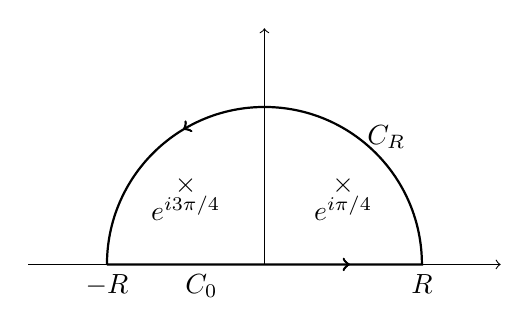
\begin{tikzpicture}
      \draw [->] (-3, 0) -- (3, 0);
      \draw [->] (0, 0) -- (0, 3);

      \draw [black, thick, ->-=0.3, ->-=0.8] (-2, 0) -- (2, 0) node [pos=0.3, below] {$C_0$} arc(0:180:2) node [pos=0.3, right] {$C_R$};

      \node [below] at (-2, 0) {$-R$};
      \node [below] at (2, 0) {$R$};

      \node at (1, 1) {$\times$};
      \node [below] at (1,1) {$e^{i\pi/4}$};
      \node at (-1,1) {$\times$};
      \node [below] at (-1,1) {$e^{i3\pi/4}$};
    \end{tikzpicture}
  \end{center}
The residue theorem gives
$$\oint_C\frac{z^2}{1+z^4}dz=2\pi i(0.25 e^{-i\pi/4}+0.25e^{-i3\pi/4})=\pi\cos\frac{\pi}{4}$$
The integration along $\gamma_R:~z=Re^{i\theta}$ gives
\begin{align}
\int_{\gamma_R}\frac{z^2}{1+z^4}dz&=\int_0^\pi\frac{R^2e^{2i\theta}}{1+R^4e^{i4\theta}}iRe^{i\theta}d\theta\nonumber\\&=\frac{iR^3}{R^4}\int_0^\pi e^{-i\theta}\bigg(1-\frac{1}{R^4}e^{-4i\theta}\bigg)^{-1}d\theta\nonumber\\&=\frac{i}{R}\int_0^\infty 1+O(R^{-4})d\theta\rightarrow 0\text{ as }R\rightarrow\infty\nonumber
\end{align}
The contour integration would then be
$$\oint_C\frac{z^2}{1+z^4}dz\rightarrow\int_{\gamma_0}\frac{z^2}{1+z^4}dz=\int_{-\infty}^\infty\frac{x^2}{1+x^4}dx=\frac{\pi}{\sqrt{2}}$$
\end{enumerate}
\item Consider $\int_C\frac{\ln z}{z^2+a^2}dz$, then the integrand has branch point singularity at 0 and $\infty$, as well as, first order poles at $x=\pm ia$. We need to choose a branch cut - say along the negative imaginary axis. We thus choose $C$ to be an indentation contour.
 \begin{center}
    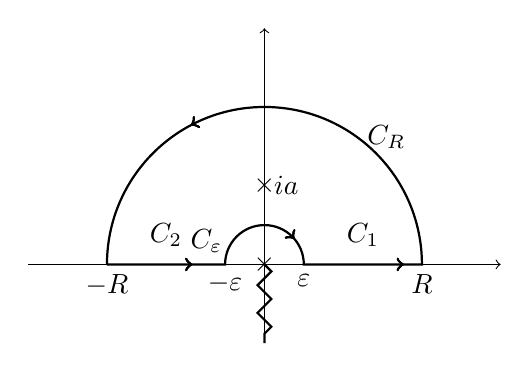
\begin{tikzpicture}
      \draw [->] (-3, 0) -- (3, 0);
      \draw [->] (0, -1) -- (0, 3);
      \draw [black, thick, ->-=0.1, ->-=0.25, ->-=0.4, ->-=0.8] (-2, 0) node [below] {$-R$} -- (-0.5, 0) node [below] {$-\varepsilon$} arc(180:0:0.5) node [pos=0.2, left] {$C_\varepsilon$} node [below] {$\varepsilon$} -- (2, 0) node [below] {$R$} arc(0:180:2) node [pos=0.3, right] {$C_R$};
 \node {$\times$};
      \node at (0,1) {$\times$};
      \node [right] at (0, 1) {$ia$};
      
        \node [circle] at (1,1){};
    \node [above] at (1.25,0.1){$C_1$};
    \node [circle] at (1,-1){};
    \node [above] at (-1.25,0.1){$C_2$};
    \draw [thick,decorate, decoration=zigzag] (0, 0) -- (0, -1);
    \end{tikzpicture}
  \end{center}
\end{enumerate}
The residue at the pole $z=+ia$ (enclosed by $C$) is
$$\res_{z=ia}\frac{\ln z}{z^2+a^2}dz=\lim_{z\rightarrow ia}\frac{\ln z}{z+ia}d\theta =\frac{\ln a+i(\pi/2)}{2ai}$$
The corresponding contributions are:
$$\int_{C_1}\frac{\ln z}{z^2+a^2}dz\rightarrow\int_0^\infty\frac{\ln x}{a^2+x^2}dx,\text{ as }\varepsilon\rightarrow 0,R\rightarrow\infty$$
$$\int_{C_R}\frac{\ln z}{z^2+a^2}dz=\int_0^\pi\frac{\ln R+i\theta}{R^2e^{2i\theta}+a^2}iRe^{i\theta}d\theta=\int_0^\pi O\bigg(\frac{\ln R}{R}\bigg)+O\bigg(\frac{1}{R}\bigg)d\theta\rightarrow 0,\text{ as }R\rightarrow\infty$$
$$\int_{C_2}\frac{\ln z}{z^2+a^2}dz=-\int_R^{\varepsilon}\frac{\ln r+i\pi}{r^2+a^2}dr\rightarrow\int_0^\infty\frac{\ln r}{r^2+a^2}dr+i\pi\int_0^\infty\frac{1}{r^2+a^2}dr,\text{ as} \varepsilon\rightarrow 0,R\rightarrow\infty$$
$$\int_{C_\varepsilon}\frac{\ln z}{z^2+a^2}dz=\int_\pi^0\frac{\ln\varepsilon+i\theta}{\varepsilon^2e^{2i\theta}+a^2}i\varepsilon e^{i\theta}d\theta=O(\varepsilon\ln\varepsilon)+O(\varepsilon)\rightarrow 0,\text{ as }\varepsilon\rightarrow 0$$
We thus have by residue theorem,
$$2\pi i\res_{z=ia}\frac{\ln z}{z^2+a^2}dz=\oint_\gamma\frac{\ln z}{z^2+a^2}dz\rightarrow 2\int_0^\infty\frac{\ln x}{x^2+a^2}dx+i\pi\int_0^\infty\frac{1}{r^2+a^2}dr$$
The real part gives
$$\int_0^\infty\frac{\ln x}{x^2+a^2}dx=\frac{\pi}{2a}\ln a$$
\end{ans}
\newpage
\begin{qns}[Transform Methods]
The response $y(t)$ of a system to a forcing function $f(t)$ is described by the second-order linear equation
\begin{equation}
    \ddot{y}+2\dot{y}+5y=f(t)\tag{*}
\end{equation}
You may assume that $f(t)$ vanishes as $t\rightarrow\pm\infty$.
\begin{enumerate}[label=(\alph*)]
\item By multiplying (*) by $e^{-i\omega t}$ and integrating, or otherwise, show that the solution to (*) can be written as
$$\tilde{y}(\omega)=-\frac{\tilde{f}(\omega)}{\omega^2-2i\omega -5}$$
where $\tilde{y}(\omega)$ and $\tilde{f}(\omega)$ are the Fourier transforms of $y(t)$ and $f(t)$, respectively.\hfill\textbf{[5]}
\item Consider the forcing function described by $\tilde{f}(\omega)=\frac{i}{\omega-2i}$.
\begin{enumerate}[label=(\roman*)]
\item Use contour integration in the complex $\omega$ plane to determine the solution $y(t)$ for both positive and negative $t$.\hfill\textbf{[12]}
\item What does this solution imply about $f(t)$ for $t < 0$? (You need not determine $f(t)$ itself.)

\hfill\textbf{[3]}
\end{enumerate}
\end{enumerate}
\end{qns}
\begin{ans}\leavevmode
\begin{enumerate}[label=(\alph*)]
\item We are essentially Fourier transforming (*) by doing integration by parts, and assert $y,\dot{y}\rightarrow 0$ as $|t|\rightarrow\infty$.
$$\int_{-\infty}^\infty(\ddot{y}+2\dot{y}+5y)e^{-i\omega t}dt=\int_{-\infty}^\infty f(t)e^{-i\omega t}dt\implies-\omega^2\tilde{y}+2i\omega\tilde{y}+5\tilde{y}=\tilde{f}(t)$$
The result follows.
\item 
\begin{enumerate}[label=(\roman*)]
\item Perform inverse Fourier transform to find the solution
$$y(t)=-\frac{1}{2\pi}\int_{-\infty}^\infty\frac{i}{\omega -2i}\frac{1}{\omega^2-2i\omega-5}e^{i\omega t}dt$$
The integrand has poles that satisfy $$\omega^2-2i\omega-5=0\implies\omega=i\pm 2$$
as well as, $\omega=2i$. To perform inverse Fourier transform, close the contour in the upper half-plane for $t>0$ and lower half-plane for $t<0$ (in order to invoke Jordan's Lemma). Close the upper half-plane ($t>0$):
$$\lim_{|\omega|\rightarrow\infty}\frac{i}{(\omega^2-2i\omega-5)(\omega-2i)}=0\implies\int_{\gamma_R}\frac{ie^{i\omega t}}{(\omega-(i+2))(\omega-(i-2))(\omega-2i)}dz\rightarrow 0,\text{ as }R\rightarrow\infty$$
\begin{center}
    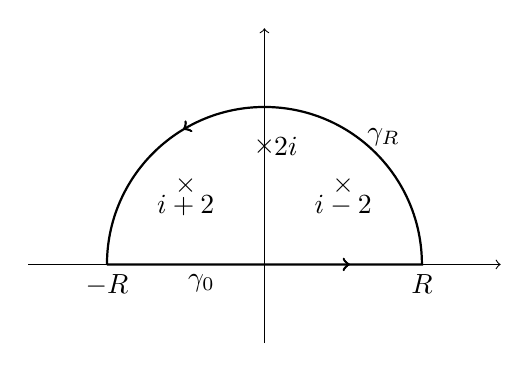
\begin{tikzpicture}
      \draw [->] (-3, 0) -- (3, 0);
      \draw [->] (0, -1) -- (0, 3);

      \draw [black, thick, ->-=0.3, ->-=0.8] (-2, 0) -- (2, 0) node [pos=0.3, below] {$\gamma_0$} arc(0:180:2) node [pos=0.3, right] {$\gamma_R$};

      \node [below] at (-2, 0) {$-R$};
      \node [below] at (2, 0) {$R$};

      \node at (0, 1.5) {$\times$};
      \node [right] at (0, 1.5) {$2i$};
      \node at (-1, 1) {$\times$};
      \node [below] at (-1, 1) {$i+2$};
      \node at (1, 1) {$\times$};
      \node [below] at (1, 1) {$i-2$};
    \end{tikzpicture}
  \end{center}
All 3 poles are enclosed when we close the upper half-plane. The residues are
$$\res_{\omega=2i}\frac{-i}{2\pi}\frac{e^{i\omega t}}{(\omega-(i+2))(\omega-(i-2))(\omega-2i)}=\lim_{\omega=2i}\frac{-i}{2\pi}\frac{e^{i\omega t}}{(\omega-(i+2))(\omega-(i-2))}=\frac{i}{10\pi}e^{-2t}$$
\begin{align}
\res_{\omega=i\pm 2}\frac{-i}{2\pi}\frac{e^{i\omega t}}{(\omega-(i+2))(\omega-(i-2))(\omega-2i)}&=\lim_{\omega=i\pm 2}\frac{-i}{2\pi}\frac{e^{i\omega t}}{(\omega-2i)(\omega-(i\mp2))}\nonumber\\&=\frac{-i}{40\pi}(2\pm i)e^{-t}e^{\pm2it}\nonumber
\end{align}
Hence, by residue theorem,
$$-\frac{1}{2\pi}\oint_C\frac{i}{\omega -2i}\frac{1}{\omega^2-2i\omega-5}e^{i\omega t}dt=2\pi i\bigg(\frac{i}{10\pi}e^{-2t}-\frac{i}{40\pi}(2+i)e^{-t}e^{2it}-\frac{i}{40\pi}(2-i)e^{-t}e^{-2it}\bigg)$$
But as $R\rightarrow\infty$, then LHS $\rightarrow y(t>0)$.\\[5pt]
Next, close the lower half-plane for $t<0$ (in order to invoke Jordan's Lemma again). But since no poles are enclosed, we expect the contour integral to be zero after invoking residue theorem. Hence, the solution is
\begin{align}
y(t)&=\left\{
        \begin{array}{ll}
      -\frac{1}{5}e^{-2t}+\frac{1}{20}e^{-t}[(2+i)e^{2it}+(2-i)e^{-2it}] & t>0 \\
      0 & t<0
        \end{array}
    \right.\nonumber\\&=
    \left\{
        \begin{array}{ll}
      -\frac{1}{5}e^{-2t}+\frac{1}{10}e^{-t}(2\cos 2t+\sin 2t) & t>0 \\
      0 & t<0
        \end{array}
    \right.\nonumber
\end{align}
\item Given that the Green's function is causal and since $y(t)=0$ for $t<0$, we expect $f(t)=0$ for $t<0$.
\end{enumerate}
\end{enumerate}
\end{ans}
\newpage
\begin{qns}[Tensors]
Let $T$ be a second-order tensor with components $T_{ij }$with respect to a Cartesian coordinate system $(x_1, x_2, x_3)$. An alternative Cartesian coordinate system $(x_1',x_2',x_3')$ is defined by $x_i'=M_{ij}x_j$.
\begin{enumerate}[label=(\alph*)]
\item What restriction is placed on the transformation matrix $M_{ij}$? How can one determine whether $(x_1',x_2',x_3')$ is a left- or right-handed coordinate system? Write down expressions for the components of $T$ in the $x_i'$ coordinate system in terms of $T_{ij}$.\hfill\textbf{[3]}
\item Show that the symmetric and antisymmetric parts of $T$ are second-order tensors.\hfill\textbf{[3]}
\item Consider the second-order tensor field $F$, with position-dependent components
$$F_{ij}=\begin{pmatrix}x_1^2&-x_1^2+x_2x_1-x_2^2&x_1-x_2\\x_1^2+x_1x_2+x_2^2&x_2^2&-x_1-x_2\\-x_1+x_2&x_1+x_2&3(x_1^2+x_2^2)\\\end{pmatrix}$$
with respect to the $x_i$ coordinates. Write down the components of the symmetric part of $F$. Determine the principal axes and corresponding principal values of the symmetric part of $F$, and describe the orientation of the principal axes geometrically.\\[5pt]
Write down the transformation matrix $M_{ij}$ that is needed to transform from the original axes to these principal axes.\hfill\textbf{[10]}
\item Decompose the tensor field $F$ introduced above as $F_{ij}=P\delta_{ij}+\hat{S}_{ij}+\hat{A}_{ij}$ , where $P$ is a scalar field, $\hat{S}_{ij}$ is symmetric and trace-free, and $\hat{A}_{ij}$ is antisymmetric. Determine whether the principal axes of $\hat{S}_{ij}$ are the same as those found in (c).\hfill\textbf{[4]}
\end{enumerate}
\end{qns}
\begin{ans}\leavevmode
\begin{enumerate}[label=(\alph*)]
\item $M$ must be orthogonal. With respect to the primed frame, if $(1,0,0)\times(0,1,0)$
\begin{itemize}
    \item $=(0,0,1)$, the system is right-handed;
    \item $=(0,0,-1)$, the system is left-handed.
\end{itemize}
$$T_{ij}'=M_{i\alpha}M_{j\beta}T_{\alpha\beta}$$
\item Any second-order tensor may be decomposed into a symmetric part and an anti-symmetric part:
$$T_{ij}=\frac{1}{2}(T_{ij}+T_{ji})+\frac{1}{2}(T_{ij}-T_{ji})$$
Now each part transforms like a second-order tensor:
$$\frac{1}{2}(T_{ij}\pm T_{ji})'=\frac{1}{2}(M_{i\alpha}M_{j\beta}T_{\alpha\beta}\pm M_{i\alpha}M_{j\beta}T_{\beta\alpha})=M_{i\alpha}M_{j\beta}\frac{1}{2}(T_{\alpha\beta}\pm T_{\beta\alpha})$$
\item The symmetric part of $F$ is 
$$S=\begin{pmatrix}x_1^2&x_1x_2&0\\x_1x_2&x_2^2&0\\0&0&3(x_1^2+x_2^2)\\\end{pmatrix}$$
By inspection, $3(x_1^2+x_2^2)$ is an eigenvalue of $S$ with eigenvector $(0,0,1)^T$. For the remaining:
$$0=\det\begin{pmatrix}x_1^2-\lambda&x_1x_2\\x_1x_2&x_2^2-\lambda\\\end{pmatrix}=(x_1^2-\lambda)(x_2^2-\lambda)-x_1^2x_2^2=-\lambda(x_1^2+x_2^2)+\lambda^2$$
The eigenvalues are thus $x_1^2+x_2^2$ and 0 with respective eigenvectors $(x_1,x_2,0)^T$ and $(x_2,-x_1,0)^T$. The transformation matrix is
$$M=\frac{1}{\sqrt{x_1^2+x_2^2}}\begin{pmatrix}x_1&x_2&0\\x_2&-x_1&0\\0&0&\sqrt{x_1^2+x_2^2}\\\end{pmatrix}$$
\item $P=\frac{\Tr(S)}{3}=\frac{4(x_1^2+x_2^2)}{3}$, and
$$\hat{S}=\begin{pmatrix}-(x_1^2+4x_2^2)/3&x_1x_2&0\\x_1x_2&-(4x_1^2+x_2^2)/3&0\\0&0&-(5x_1^2+5x_2^2)/3\\\end{pmatrix},~\hat{A}=\begin{pmatrix}0&-x_1^2-x_2^2&x_1-x_2\\x_1^2+x_2^2&0&-x_1-x_2\\x_2-x_1&x_1+x_2&0\\\end{pmatrix}$$
Let $\mathbf{e_i}$ be one of the eigenvectors along the principal axes, then
$$\hat{S}\mathbf{e_i}=S\mathbf{e_i}-P\mathbf{e_i}=(\lambda_i-P)\mathbf{e_i}$$
\end{enumerate}
\end{ans}
\begin{qns}[Normal Modes]
Three climbers have fallen from an overhanging cliff and are now suspended by their identical elastic safety ropes. The tension in each rope is given by $T(L) = k(L − L_0)$, for $L > L_0$, where $k$ is a constant and $L_0$ is the unstretched length of each rope. Climber 1 is suspended from the cliff top by rope 1 with stretched length $L_1(t)$. The other two climbers are suspended directly from climber 1. Climber 2 is suspended from climber 1 by rope 2 with stretched length $L_2(t)$, while climber 3 is suspended from climber 1 by rope 3 with stretched length $L_3(t)$. The climbers have masses $m_1$, $m_2$, and $m_3$, respectively. The mass of the ropes is negligible.
\begin{enumerate}[label=(\alph*)]
\item Write down expressions for the potential and kinetic energies of the system and hence determine its Lagrangian. (Take the gravitational acceleration to be $g$ and remember to include the elastic potential energy.)\hfill\textbf{[4]}
\item Use the Euler–Lagrange equations to derive the equations of motion for $L_i$. Show that, at equilibrium, the lengths of the ropes are given by $L_i = \hat{L}_i$ where\hfill\textbf{[5]}
$$\hat{L}_1=L_0+\frac{g}{k}(m_1+m_2+m_3)$$
$$\hat{L}_2=L_0+\frac{g}{k}m_2$$
$$\hat{L}_3=L_0+\frac{g}{k}m_3$$
\item Let $y_i=L_i-\hat{L}_i$ be a small departure from equilibrium. Show that\hfill\textbf{[2]}
$$\begin{pmatrix}m_1+m_2+m_3&m_2&m_3\\m_2&m_2&0\\m_3&0&m_3\\\end{pmatrix}\begin{pmatrix}\ddot{y}_1\\\ddot{y}_2\\\ddot{y}_3\\\end{pmatrix}+\begin{pmatrix}k&0&0\\0&k&0\\0&0&k\\\end{pmatrix}\begin{pmatrix}y_1\\y_2\\y_3\\\end{pmatrix}=\begin{pmatrix}0\\0\\0\\\end{pmatrix}$$
\item Assume, now, that all climbers have equal mass $m$. Show that one normal mode of oscillation has frequency $\omega=\sqrt{k/m}$ and that climber 1 is stationary in this mode. For this case, describe the motion of the other two climbers. Determine also the frequencies of the other two modes of oscillation.\hfill\textbf{[9]}
\end{enumerate}
\end{qns}
\newpage
\begin{ans}\leavevmode
\begin{enumerate}[label=(\alph*)]
\item We define the positions of the 3 climbers relative to the top of the cliff are $z_1=-L_1$, $z_2=-L_2-L_1$, $z_3=-L_1-L_3$. The Lagrangian is $\mathcal{L}=T-V$. The kinetic energy is
$$T=\frac{1}{2}m_1\dot{z}_1^2+\frac{1}{2}m_2\dot{z}_2^2+\frac{1}{2}m_3\dot{z}_3^2$$
The potential energy is
$$V=g(m_1z_1+m_2z_2+m_3z_3)+\frac{k}{2}[(L_1-L_0)^2+(L_2-L_0)^2+(L_3-L_0)^2]$$
Then the Lagrangian is $\mathcal{L}[L_i,\dot{L}_i;t]$:
\begin{eqnarray}
&&\frac{1}{2}(m_1\dot{L}_1^2+m_2(\dot{L}_2+\dot{L}_1)^2+m_r(\dot{L}_3+\dot{L}_1)^2)\nonumber\\&&+g(m_1L_1+m_2(L_2+L_1)+m_3(L_1+L_3))-\frac{1}{2}k((L_1-L_0)^2+(L_2-L_0)^2+(L_3-L_0)^2)\nonumber
\end{eqnarray}
\item To extremize the Lagrangian, it must satisfy the Euler-Lagrange equation $\frac{d}{dt}\frac{\partial\mathcal{L}}{\partial\dot{L}_i}=\frac{\partial\mathcal{L}}{\partial L_i}$ $\forall i=1,2,3$:
$$\frac{d}{dt}(m_1\dot{L}_1+m_2(\dot{L}_1+\dot{L}_2)+m_3(\dot{L}_1+\dot{L}_3))=g(m_1+m_2+m_3)-k(L_1-L_0)$$
$$\frac{d}{dt}(m_2(\dot{L}_2+\dot{L}_1))=gm_2-k(L_2-L_0)$$
$$\frac{d}{dt}(m_3(\dot{L}_3+\dot{L}_1))=gm_3-k(L_3-L_0)$$
In equilibrium, $\frac{d}{dt}\frac{\partial\mathcal{L}}{\partial\dot{L}_i}=0$, so $k(\hat{L}_1-L_0)=g(m_1+m_2+m_3)$, $k(\hat{L}_2-L_0)=gm_2$ and $k(\hat{L}_3-L_0)=gm_3$, which is the desired result.
\item Let $y_i=L_i-\hat{L}_i$ and $\dot{y}_i=\dot{L}_i$ $\forall i$, so rearranging gives
$$\ddot{y}_1(m_1+m_2+m_3)+\ddot{y}_2+\ddot{y}_3m_3=-ky_1$$
$$\ddot{y}_1m_2+\ddot{y}_2m_2=0+ky_2$$
$$\ddot{y}_3m_3+\ddot{y}_3m_3=0+ky_3$$
This is equivalent to the desired matrix.
\item We look for solutions of the form $y_i=\text{Re}[a_ie^{i\omega t}]$, then we need solve the following equation to obtain $\omega^2$:
$$0=\det\begin{pmatrix}3-\frac{k}{m\omega^2}&1&1\\1&1-\frac{k}{m\omega^2}&0\\1&0&1-\frac{k}{m\omega^2}\\\end{pmatrix}=\bigg(1-\frac{k}{m\omega^2}\bigg)\bigg(\frac{k^2}{m^2\omega^4}-4\frac{k}{m\omega^2}+1\bigg)$$
The solutions are $\frac{k}{m\omega^2}=1,2\pm\sqrt{3}$ and hence $\omega_0:=\sqrt{\frac{k}{m}}$ and $\omega_\pm=\sqrt{\frac{k}{m}}\frac{1}{\sqrt{2\pm\sqrt{3}}}$.
For the $\omega_0$ mode, let the eigenvector be $(a,b,c)^T$, then
$$0=\begin{pmatrix}2&1&1\\1&0&0\\1&0&0\\\end{pmatrix}\implies a=0,b=-c$$
The other two climbers oscillate in anti-phase with equal amplitude, while the first climber is stationary.
\end{enumerate}
\end{ans}
\newpage
\begin{qns}[Group Theory]\leavevmode
\begin{enumerate}[label=(\alph*)]
\item Let $H$ be a subgroup of a finite group $G$. Define the left coset $gH$ of $H$ for an element $g\in G$. Prove that the left cosets of $H$ partition $G$.\hfill\textbf{[6]}
\item Show that the set of all real 3 $\times$ 3 matrices with elements
\begin{equation}
    \begin{pmatrix}1&x&y\\0&1&z\\0&0&1\\\end{pmatrix}\tag{*}
\end{equation}
forms a group under matrix multiplication. Show further that the subset of matrices with $x = z = 0$ forms a normal subgroup.\hfill\textbf{[6]}
\item 
\begin{enumerate}[label=(\roman*)]
\item Now suppose that $x$, $y$, and $z$ are integers mod 4 (e.g., 5 mod 4 $=$ 1). Show that the set of matrices of the form in (*) is a finite group $G$ under matrix multiplication with arithmetic modulo 4, and determine the order of $G$.\hfill\textbf{[4]}
\item Show that the subset of such matrices given by $x = z$ defines an Abelian subgroup $H$. Determine the order of $H$. How many distinct left cosets of $H$ are there in $G$?\hfill\textbf{[4]}
\end{enumerate}
\end{enumerate}
\end{qns}
\begin{ans}\leavevmode
\begin{enumerate}[label=(\alph*)]
\item A left coset of $H\leq G$ is 
$$gH:=\{g'\in G|g'=g*h\text{ for some }h\in H\}$$
for some $g\in G$. The set of left cosets is $G/H$. These cosets are either disjoint or identical. Let $g_1H$ and $g_2H$ only share a single element but $g_1\neq g_2$, then $$g_1h_i=g_2h_j\implies g_1=g_2h_jh_i^{-1}=g_2h_k$$
where $h_i,h_j\in H$, $h_k=h_jh_i^{-1}\in H$. So, $g_1H=g_2h_kH=g_2H$. Take each element in $G$ in turn and pre-multiply $H$ by that element, then at least one coset contains each element in $G$. Each element is thus in one coset and this coset is the only one as shown earlier, then the cosets partition the group.
\item We let the set of this matrix is $G$. Check group axioms:
\begin{itemize}
    \item closure: Let $A,A'\in G$,
    $$AA'= \begin{pmatrix}1&x&y\\0&1&z\\0&0&1\\\end{pmatrix} \begin{pmatrix}1&x'&y'\\0&1&z'\\0&0&1\\\end{pmatrix}= \begin{pmatrix}1&x+x'&y'+xz'+y\\0&1&z+z'\\0&0&1\\\end{pmatrix}\in G$$
    \item associativity: matrix multiplication is associative.
    \item identity: $x=0=y=z\in\mathbb{R}$, so $I\in G$.
    \item Inverse: For $A\in G$, we have $x+x'=0$, $z+z'=0$, $x'+y'+xz=0$. So, $$A^{-1}= \begin{pmatrix}1&-x&-y+xz\\0&1&-z\\0&0&1\\\end{pmatrix}\in G$$
\end{itemize}
Let $H$ to be the set of all real $3\times 3$ matrices of the form ($x=z=0$):
$$\begin{pmatrix}1&0&y\\0&1&0\\0&0&1\\\end{pmatrix}$$
For $H$, trivial to show it inherits associativity and identity ($y=0\in\mathbb{R}$) and has an inverse ($y\in\mathbb{R}\implies -y\in\mathbb{R}$). This satisfies subgroup axioms, so $H\leq G$.\\[5pt]
To check this form a normal subgroup in $G$, we need to show each element in $H$ commutes with every element in $G$ (so each element in $H$ is in their conjugacy classes, hence $H$ is built from the entire conjugacy classes, and hence normal in $G$):
$$ \begin{pmatrix}1&0&y'\\0&1&0\\0&0&1\\\end{pmatrix} \begin{pmatrix}1&x&y\\0&1&z\\0&0&1\\\end{pmatrix}= \begin{pmatrix}1&x&y+y'\\0&1&z\\0&0&1\\\end{pmatrix}=\begin{pmatrix}1&x&y\\0&1&z\\0&0&1\\\end{pmatrix}\begin{pmatrix}1&0&y'\\0&1&0\\0&0&1\\\end{pmatrix}$$
\item Let $\mathbb{Z}_4=\{0,1,2,3\}$ be the set of integers modulo 4. The groups $G$ and $H\leq G$ are of the same forms but this time over $\mathbb{Z}_4$ and not $\mathbb{R}$.
\begin{enumerate}[label=(\roman*)]
\item Check the group axioms (all binary operations are defined modulo 4):
\begin{itemize}
    \item closure: closed since $x,x'\in\mathbb{Z}_4\implies x+x'\in\mathbb{Z}_4$; $x,y,y',z,z'\in\mathbb{Z}_4\implies y+xz'+y'\in\mathbb{Z}_4$ and $z+z'\in\mathbb{Z}_4$.
    \item associativity: matrix multiplication is still associative over $\mathbb{Z}_4$.
    \item identity: the same identity exists since $0\in\mathbb{Z}_4$.
    \item inverse: when $x+x'=0$, $y'+xz'+y=0$ and $z+z'=0$, we can find solutions $x',y',z'\in\mathbb{Z}_4$, so we have an inverse.
\end{itemize}
There are 4 possibilities for $x,y,z$ and so $4^3$ distinct matrices. The order of $G$ is $4^3=64$.
\item Again, similar to part (b) and (ci), $H$ will satisfy the subgroup axioms over $\mathbb{Z}_4$. The order is now $4^2=16$. By Lagrange's theorem, the number of distinct cosets of $H$ in $G$ is $\frac{|G|}{|H|}=4$.
\end{enumerate}
\end{enumerate}
\end{ans}
\begin{qns}[Group Theory]
Let $G$ and $G_0$ be finite groups.
\begin{enumerate}[label=(\alph*)]
\item Let $\Phi:G\rightarrow G'$ be a homomorphism. Define the kernel $K$ of $\Phi$. Prove that $K$ is a normal subgroup of $G$.\hfill\textbf{[5]}
\item Define the conjugacy class of $g\in G$. Prove that any normal subgroup of $G$ is a union of conjugacy classes.\hfill\textbf{[3]}
\item What is meant by the cycle structure of a permutation? List the possible cycle structures for elements of $\Sigma_3$ (the permutation group for three objects).\hfill\textbf{[3]}
\item Assume that $\Phi:\Sigma_3\rightarrow G'$ is a homomorphism that is onto, i.e., any element of $G'$ can be written as $\Phi(g)$ for some $g\in\Sigma_3$. Determine the possible forms of $K$ (the kernel of $\Phi$) and hence, or otherwise, prove that $G'$ must be isomorphic to one of $\Sigma_3$, $C_2$ (the cyclic group of order 2), or the trivial group $\{I\}$.\hfill\textbf{[9]}
\end{enumerate}
[You may assume that two elements of $\Sigma_3$ belong to the same conjugacy class if, and only if, they have the same cycle structure.]
\end{qns}
\begin{ans}\leavevmode
\begin{enumerate}[label=(\alph*)]
\item The kernel of a homomorphism $\Phi:~G\rightarrow G'$ is
$$K=\{h\in G|~\Phi(h)=e_{G'}\text{ for some }h\in G\}$$
First check $K\leq G$ (subgroup axioms):
\begin{itemize}
    \item closed: let $k_1,k_2\in K$, then $\Phi(k_1)=e_{G'}=\Phi(k_2)$. We have
    $$e_{G'}=\Phi(k_1)\Phi(k_2)=\Phi(k_1k_2)\implies k_1k_2\in K$$
    \item associativity: inherited from $G$.
    \item identity: $e_G\in K$ since $\Phi(e_G)=e_{G'}$.
    \item inverse: for $k\in K$,
    $$e_{G'}=\Phi(e_G)\Phi(k^{-1}k)=\Phi(k^{-1}k)=\Phi(k^{-1})\Phi(k)=\Phi(k^{-1})e_{G'}\implies k^{-1}\in K$$
\end{itemize}
next, check $K$ is a normal subgroup of $G$, i.e. $K\lhd G$. Let $k\in K$ and if $g\in G$,
$$\Phi(gkg^{-1})=\Phi(g)\Phi(k)\Phi(g^{-1})=\Phi(g)e_{G'}\Phi(g^{-1})=e_{G'}\implies gkg^{-1}\in K$$
\item The conjugacy class of $g\in G$, written as $\ccl(g)$ is
$$\ccl(g)=\{k\in G\text{ such that }k=hgh^{-1}\text{ for some }h\in G\}$$
$H$ is a normal subgroup of $G$ if for every $h\in H$ and $g\in G$, we have $ghg^{-1}\in H$. As a result, $Hg_i=g_iH$ $\forall g_i\in G$, then $g_iHg_i^{-1}=H$. If $h_i\in H$ but does not contain every element to which $h_i$ was conjugate, then the above will not be true. But it is, so $H$ does contain every element to which $h_i$ was conjugate to. Hence, $H$ is a union of conjugacy classes.
\newpage
\item Given a list $a_1,a_2,\dots,a_k\in\{1,2,\dots,n\}$ of distinct elements, then the $k$-cycle $(a_1a_2\dots a_k)\in \Sigma_n$ is the permutation given by
$$(a_1a_2\dots a_k)(i)=
\left\{
        \begin{array}{ll}
      a_{j+1} & i=a_j\text{ for }j<k \\
      a_1 & i=a_k\\
      i & i\neq a_j\text{ for any }j
        \end{array}
    \right.$$
i.e. the $k$-cycle moves every element in the subset $\{a_1,a_2,\dots,a_k\}\subset\{1,2,\dots,n\}$ and fixes every element outside of this subset. Every permutation $\sigma\in\Sigma_n$ can be written as a composition of disjoint cycles. The possible cycle structures of $\Sigma_3$ are $(.)(.)(.)$, $(..)(.)$ and $(...)$.
\item $\Sigma_3$ consists of
$$\Sigma_3=\{\Id=(1)(2)(3),(12)(3),(23)(1),(13)(2),(123),(132)\}$$
$\Id$ has order 1, $(12)(3),(23)(1),(13)(2)$ have order 2 each, $(123),(132)$ have order 3 each. The group table of $\Sigma_3$ is
$$\vbox{\tabskip0.5em\offinterlineskip
    \halign{\strut$#$\hfil\ \tabskip1em\vrule&&$#$\hfil\cr
    & \Id & (12)(3) & (23)(1) & (13)(2) & (123) & (132)     \cr
    \noalign{\hrule}\vrule height 12pt width 0pt
    \Id  & \Id & (12)(3)   & (23)(1)   & (13)(2) & (123) & (132)     \cr
     (12)(3) & (12)(3) & \Id & (123)   & (132)   & (23)(1) & (13)(2)     \cr
    (23)(1) & (23)(1)   & (132)   & \Id  & (123) & (13)(2) & (12)(3)      \cr
    (13)(2) & (13)(2)  & (123)   & (132) & \Id   & (12)(3) & (23)(1)      \cr
    (123) & (123) & (13)(2) & (12)(3) & (23)(1) & (132) & \Id \cr
    (132) & (132)  & (23)(1)   & (13)(2)   & (12)(3)   & \Id & (123)     \cr
}}$$
The subgroups of $\Sigma_3$ are the trivial subgroup, $\Sigma_3$ itself, $\{\Id,(12)(3)\}$, $\{\Id,(23)(1)\}$, $\{\Id,(13)(2)\}$, $\{\Id,(123),(132)\}$. None of the order 2 subgroups are normal in $\Sigma_3$, for instance: $$(132)(12)(3)(132)^{-1}=(13)(2)\neq(12)(3)$$
so order 2 subgroups can't be $\Ker\Phi$. In fact, only elements of the same order may be conjugate to each other (hence same cycle structure), say $g_1$, $g_2$ where $\ord(g_1)=p$ and $\ord(g_2)=q$, then
$$g_1=hg_2h^{-1}\implies e=g_1^p=hg_2^ph^{-1}\implies g_2^p=h^{-1}eh=e$$
so $q$ is a factor of $p$. Similarly, can show $p$ is a factor of $q$. Hence, $p=q$. In conclusion, the only normal subgroups are $\{e\}$, $\Sigma_3$ and $\{\Id,(12),(132)\}$. These are possible forms of $\Ker\Phi$ by part (a).\\[5pt]
Each coset of $K$ in $G$ can be put into one-to-one correspondence to the elements in $G$, which means the number of cosets of $K$ is the number of elements in $G$. We can show this: suppose two cosets map to the same elements in $G'$, then
$$\Phi(g_iK)=\Phi(g_jK)\implies \Phi(g_j^{-1}g_iK)=\Phi(g_j^{-1})\Phi(g_iK)=\Phi(g_j^{-1})\Phi(g_jK)=\Phi(K)=I$$
Hence, $g_j^{-1}g_iK=K\implies g_iK=g_k$, i.e. the two cosets are the same. Hence, the order of the image of an element must be a factor of the order of the pre-image.
\begin{itemize}
\item For the mapping whose kernel is $\Sigma_3$, everything is mapped to the identity so This corresponds to $G'=\{\Id\}$.
\item For the mapping whose kernel is $\{\Id\}$, this is an one-to-one onto mapping, so $G$ and $G'$ are isomorphic, i.e. $G\simeq G'$.
\item For the mapping whose kernel is $\{\Id,(123),(132)\}$. The above shows that there are only two elements in $G'$, hence $G'=C_2$ (cyclic).
\end{itemize}
\end{enumerate}
\end{ans}
\newpage
\begin{qns}[Representation Theory]
Consider the $D_6$ dihedral group
$$G=\{I,R,R^2,R^3,R^4,R^5,m_1,m_2,m_3,m_4,m_5,m_6\}$$
with structure defined by the group table
$$\vbox{\tabskip0.5em\offinterlineskip
    \halign{\strut$#$\hfil\ \tabskip1em\vrule&&$#$\hfil\cr
    ~   & I   & R   & R^2 & R^3 &R^4 & R^5 & m_1& m_2&m_3 & m_4&m_5& m_6    \cr
    \noalign{\hrule}\vrule height 12pt width 0pt
     I & I   & R   & R^2 & R^3 &R^4 & R^5 & m_1& m_2&m_3 & m_4&m_5& m_6    \cr
     R & R  & R^2   & R^3 & R^4 &R^5 & I & m_2& m_3&m_4 & m_5&m_6& m_1    \cr
     R^2 & R^2  & R^3   & R^4 & R^5 &I & R & m_3& m_4&m_5 & m_6&m_1& m_2    \cr
     R^3 & R^3  & R^4   & R^5 & I &R & R^2 & m_4& m_5&m_6 & m_1&m_2& m_3    \cr
     R^4 & R^4  & R^5   & I & R &R^2 & R^3 & m_5& m_6&m_1 & m_2&m_3& m_4    \cr
     R^5 & R^5  & I   & R & R^2 &R^3 & R^4 & m_6& m_1&m_2 & m_3&m_4& m_5    \cr
     m_1 & m_1  & m_6   & m_5 & m_4 & m_3 & m_2 & I& R^5&R^4 & R^3&R^2& R    \cr
     m_2  &m_2 & m_1   & m_6 & m_5 &m_4 & m_3 & R& I&R^5 & R^4 &R^3& R^2    \cr
     m_3  &m_3  & m_2   & m_1 & m_6 &m_5 & m_4 & R^2& R&I & R^5&R^4& R^3    \cr
     m_4  &m_4 & m_3   & m_2 & m_1 &m_6 & m_5 & R^3& R^2&R & I&R^5& R^4    \cr
     m_5  &m_5 & m_4   & m_3 & m_2 &m_1 & m_6 & R^4& R^3&R^2 & R&I& R^5    \cr
     m_6  &m_6  & m_5   & m_4 & m_3 &m_2 & m_1 & R^5& R^4&R^3 & R^2&R& I    \cr
}}$$
\begin{enumerate}[label=(\alph*)]
\item What do the generators $R$ and $m_1$ represent geometrically? Give an expression for each of the group members in terms of the generators $\{R,m_1\}$.\hfill\textbf{[2]}
\item Identify all the subgroups of order 2 and 3. Are any of these subgroups cyclic? \hfill\textbf{[5]}
\item Explain how to construct a faithful representation of G using $2\times 2$ orthogonal matrices. Give matrices corresponding to $R$, $m_1$, and $m_2$ in such a representation.\hfill\textbf{[4]}
\item Write down the regular representation $D(g)$ for $g = m_4$ and hence or otherwise derive an expression for $[D(m_4)]^n$ for any integer $n$.\hfill\textbf{[5]}\\[5pt]
[Reminder: the regular representation is a set of $|G|\times|G|$ permutation matrices each with $|G|$ non-zero elements.]
\item State the characters of the representations used above in (c) and (d). \hfill\textbf{[4]}
\end{enumerate}
\end{qns}
\newpage
\begin{ans}\leavevmode
\begin{enumerate}[label=(\alph*)]
\item $R$ geometrically represents a rotation about the origin in a plane with an angle of $\frac{2\pi}{6}$. $m_1$ geometrically represents a reflection about any line passing through the origin (without loss of generality, can be $x$-axis).
$$I=R^6=m_1^2,\quad R^p=R^p,~p\in[1,5],\quad m_1=m_1,\quad m_i=m_1R^{i-1}=R^{7-i}m_1,~i\in[2,6]$$
\item The subgroups of order 2 are $\{I,m_i\}$ $\forall i$ and $\{I,R^3\}$. The subgroup of order 3 is $\{I,R^2,R^4\}$. Both are cyclic groups.
\item Consider the action of the group elements on a reference vector $e:=(x,y)^T$, then
$$I=\begin{pmatrix}1&0\\0&1\\\end{pmatrix},~R=\begin{pmatrix}\cos\pi/6 &\sin\pi/6\\-\sin\pi/6&\cos\pi/6\\\end{pmatrix},~m_1=\begin{pmatrix}-1&0\\0&1\\\end{pmatrix},~m_2=m_1R=\begin{pmatrix}-\sqrt{3}/2&-1/2\\-1/2&\sqrt{3}/2\\\end{pmatrix}$$
\item In terms of the 12-dimensional basis (where $e$ was the reference vector): 
$$\{e,Re,R^2e,R^3e,R^4e,R^5e,m_1e,m_2e,m_3e,m_4e,m_5e,m_6e\}$$
Each matrix element (row $g$ and column $g'$) is $\langle ge|D|g'e\rangle$.
\setcounter{MaxMatrixCols}{20}
$$D(R)=\begin{pmatrix}
& & & & &1 & & & & & &\\
& & & &1 & & & & & & &\\
& & &1 & & & & & & & &\\
& &1 & & & & & & & & &\\
& 1& & & & & & & & & &\\
1& & & & & & & & & & &\\
& & & & & & &1 & & & &\\
& & & & & & & &1 & & &\\
& & & & & & & & &1 & &\\
& & & & & & & & & &1 &\\
& & & & & & & & & & &1\\
& & & & & &1 & & & & &\\
\end{pmatrix}$$
$$D(m_4)=\begin{pmatrix}
& & & & & & & & &1& &\\
& & & & & & & &1& & &\\
& & & & & & &1& & & &\\
& & & & & &1& & & & &\\
& & & & & & & & & & &1\\
& & &1& & & & & & & &\\
& & & &1& & & & & & &\\
& & & & &1& & & & & &\\
& & & & & & & & & & &\\
1& & & & & & & & & & &\\
&1& & & & & & & & & &\\
& &1& & & & & & & & &\\
\end{pmatrix}
$$
Since the representations are homomorphisms, we expect, $D(m_4)^{n}=D(m_4^n)=D(m_4^{\mod(n,2)})$ where $m_4$ raised to even power is identity (we have $D(I)=I$) and $m_4$ raised to odd power is $m_4$. 
\item The character for two-dimensional irreducible representation (in part (c)) is
$$\bigg\{2,2\cos\frac{\pi}{6},2\cos\frac{\pi}{3},2\cos\frac{\pi}{2},2\cos\frac{2\pi}{3},2\cos\frac{5\pi}{6},0,0,0,0,0,0\bigg\}$$
The six mirrors have zero trace. For regular representation (in part (d)), the character is
$$\{12,0,0,0,0,0,0,0,0,0,0,0\}$$
where only the identity has non-zero trace.


\end{enumerate}
\end{ans}
\newpage
\section{2016}
\subsection{Paper 1}
\begin{qns}[Vector Calculus]\leavevmode
\begin{enumerate}[label=(\alph*)]
    \item State the divergence theorem for a vector field $\mathbf{F}(x, y, z)$.\hfill \textbf{[2]}
    \item Let the surface S be defined as $S=S_1\cup S_2\cup S_3$, where
$$S_1=\{(x,y,z)~:x^2+y^2=2-z,~1\leq z\leq 2\}$$
$$S_2 =\{(x, y, z) :~x^2 + y^2 = 1,~0\leq z\leq  1\},$$
$$S_3 =\{(x, y, z) :~z = 0,~x^2 + y^2\leq 1\}$$
Sketch all four surfaces.\hfill \textbf{[4]}
\item Given that $\mathbf{F}(x, y, z) = (2xy+x^6, −y^2+y^4, z)$, find $\oint_S\mathbf{F}\cdot d\mathbf{S}$, where $d\mathbf{S}$ is an element of vector area pointing in the direction of the outward normal to $S$.\hfill \textbf{[14]}
\end{enumerate}
\end{qns}
\begin{ans}\leavevmode
\begin{enumerate}[label=(\alph*)]
    \item If $\mathbf{F}=\mathbf{F}(\mathbf{x})$ be a continuously differentiable vector field and $V$ is a volume with a piecewise regular boundary $\partial V$, then divergence theorem states
$$\int_V\boldsymbol{\nabla}\cdot\mathbf{F}dV=\int_{\partial V}\mathbf{F}\cdot d\mathbf{S}$$
where the normal to $\partial V$ points outwards from $V$.
\item $S_3$ is the bottom circular base of the cylindrical curved surface $S_2$. $S_1$ is a parabolic cap on top of $S_2$.
\begin{figure}[H]
    \centering
    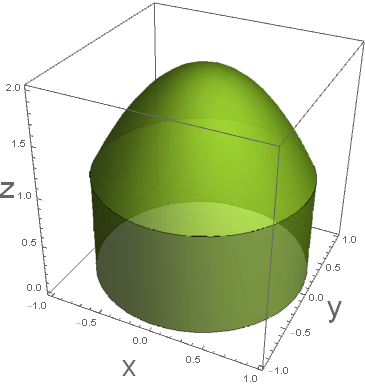
\includegraphics[scale=0.5]{2016P1Q1.png}
    %\caption{}
\end{figure}
\item The divergence of $\mathbf{F}$ is
$$\boldsymbol{\nabla}\cdot\mathbf{F}=2y+6x^5-2y+4y^3+1=6r^5\cos^5\theta+4r^3\sin^3\theta+1$$ We then invoke divergence theorem:
$$\oint_S\mathbf{F}\cdot d\mathbf{S}=\int_V\boldsymbol{\nabla}\cdot\mathbf{F}dV=\int_0^1\int_0^{2-r^2}\int_{-\pi}^\pi 6r^6\cos^5\theta+4r^4\sin^3\theta+r d\theta dzdr=2\pi\int_0^1r(2-r^2)dr=\frac{3}{2}\pi$$
where integrate odd power of trigonometric functions over integer number of cycles gives zero.
\end{enumerate}

\end{ans}
\newpage
\begin{qns}[Partial Differential Equation]
A string of uniform density per unit length $\rho$ is stretched under tension along the $x$-axis and undergoes small transverse oscillations in the $(x, y)$ plane with amplitude $y(x, t)$. The waves in the string travel with velocity $c$ and the equation of motion satisfied by $y(x, t)$ is
$$\frac{1}{c^2}\frac{\partial^2y}{\partial t^2}=\frac{\partial^2y}{\partial x^2}$$
\begin{enumerate}[label=(\alph*)]
\item If the string is fixed at $x = 0$ and $x = L$, derive the general separable solution for the amplitude $y(x, t)$.\hfill\textbf{[9]}
\item For $t < 0$ the string is at rest. At $t = 0$ the string is struck by a hammer in the interval $[\ell-a/2,\ell+a/2]$, the distance being measured from one end. The effect of the hammer is to impart a constant velocity $v$ to the string inside the interval and zero velocity outside the interval. Calculate the proportion of the total energy given to the string in each mode.\\[5pt]
[You may assume the kinetic energy formula $K.E.=\int_0^L\frac{\rho}{2}(\partial y/\partial t)^2dx$.]\hfill\textbf{[9]}
\item If $\ell=L/5$ and $a = L/7$, identify all the modes of the string which are not excited by the hammer.\hfill\textbf{[2]}
\end{enumerate}
\end{qns}
\begin{ans}\leavevmode
\begin{enumerate}[label=(\alph*)]
\item Since the boundary condition is homogeneous, we can use separation of variables $y=X(x)T(t)$.
$$\frac{T''}{T}=c^2\frac{X''}{X}=-\lambda^2$$
where the minus sign was chosen and $\lambda\neq 0$ due to the boundary conditions $y(0,t)=y(L,t)=0$ $\forall t$. We have $X\sim\sin\frac{\lambda}{c}x$ and $T(t)\sim c_3\sin\lambda t+c_4\cos\lambda t$. We require $\lambda=\frac{n\pi c}{L}$ such that $n\in\mathbb{N}$. Then, we have the general solution to be
$$y(x,t)=\sum_{n=1}^\infty\sin\frac{n\pi x}{L}\bigg(A_n\cos\frac{n\pi ct}{L}+B_n\sin\frac{n\pi ct}{L}\bigg)$$
\item For $t<0$, the string is at rest, so $A_n=0$ $\forall n$. The initial velocity $g(x)=v$ for $x\in[\ell-0.5a,\ell+0.5a]$ and zero elsewhere. We have $g(x)=\frac{\partial y}{\partial t}|_{t=0}=\sum_{n=1}^\infty\sin\frac{n\pi x}{L}B_n\frac{n\pi c}{L}$. Then, the Fourier coefficients will be
$$B_n\frac{n\pi c}{L}=\frac{2}{L}\int_0^Lg(x)dx\implies B_n=\frac{L}{n\pi c}\frac{2}{L}\int_{\ell-0.5a}^{\ell+0.5a}v\sin\frac{n\pi x}{L}dx=-\frac{4vL}{n^2\pi^2c}\sin\frac{n\pi a}{2L}\sin\frac{n\pi\ell}{L}$$
The kinetic energy for the $n$th mode is
\begin{eqnarray}
K_n&=&\frac{1}{2}\rho\int_0^Lg(x)^2\sin^2\frac{n\pi ct}{L}dx\nonumber\\&=&\frac{1}{2}\rho\int_0^L\bigg(B_n\frac{n\pi c}{L}\bigg)^2\sin^2\frac{n\pi x}{L}\sin^2\frac{n\pi ct}{L}dx\nonumber\\&=&\frac{4\rho v^2}{n^2\pi^2}\sin^2\frac{n\pi ct}{L}\sin^2\frac{n\pi a}{2L}\sin^2\frac{n\pi \ell}{L}\bigg[x-\frac{L}{2\pi n}\sin^2\frac{n\pi x}{L}\bigg]_0^L\nonumber\\&=&\frac{4\rho Lv^2}{n^2\pi^2}\sin^2\frac{n\pi ct}{L}\sin^2\frac{n\pi a}{2L}\sin^2\frac{n\pi \ell}{L}\nonumber
\end{eqnarray}
The total energy is the maximum of kinetic energy which is $\frac{4\rho Lv^2}{n^2\pi^2}\sin^2\frac{n\pi a}{2L}\sin^2\frac{n\pi l}{L}$. The total energy imparted is $\int_0^L\frac{1}{2}\rho v^2dx=\frac{1}{2}\rho v^2\int_{\ell-a/2}^{\ell+a/2}dx=\frac{1}{2}\rho av^2$. The ratio will be $\frac{8L}{an^2\pi^2}\sin^2\frac{n\pi a}{2L}\sin^2\frac{n\pi\ell}{L}$.
\item If the coefficient $B_n$ is zero, that mode is not excited. For $\ell=\frac{L}{5}$, $a=\frac{L}{7}$, 
$$B_n=-\frac{4vL}{n^2\pi^2c^2}\sin\frac{n\pi}{14}\sin\frac{n\pi}{5}$$
We thus require to be $n=0$ (mod 5) or (mod 14), i.e. a multiple of either 5 or 14.
\end{enumerate}
\end{ans}
\newpage
\begin{qns}[Green's Functions]
Consider the linear differential operator $\mathcal{L}$ defined by
$$\mathcal{L}y=-\frac{d^2y}{dx^2}+y$$
on the interval $0\leq x<\infty$. The boundary conditions are given by $y(0) = 0$ and $\lim_{x\rightarrow\infty}y(x)=0$.
\begin{enumerate}[label=(\alph*)]
\item  Find the Green’s function $G(x,\xi)$ for $\mathcal{L}$ satisfying these boundary conditions. Hence, or otherwise, obtain the solution of
$$\mathcal{L}y=
\left\{
        \begin{array}{ll}
      1 & 0\leq x<\mu \\
      0 & \mu<x<\infty
        \end{array}
    \right.$$
subject to the above boundary conditions, where $\mu$ is a positive constant.\hfill\textbf{[14]}
\item Show that your piecewise solution is continuous at $x=\mu$ and has the value \hfill\textbf{[6]}
$$y(\mu)=\frac{1}{2}(1+e^{-2\mu}-2e^{-\mu})$$
\end{enumerate}
\end{qns}
\begin{ans}\leavevmode
\begin{enumerate}[label=(\alph*)]
    \item The homogeneous solutions are $e^x$ and $e^{-x}$. The corresponding Green's function satisfy 
    $$\mathcal{L}G=-\frac{\partial^2G(x,\xi)}{\partial x^2}+G(x,\xi)=\delta(x-\xi),\quad G(0,\xi)=0,~\lim_{x\rightarrow\infty}G(x,\xi)=0$$
    Integrate around an infinitesimal region about $x=\xi$, we obtain the jump condition $[G']_{\xi^-}^{\xi^+}=1$. $G$ is continuous everywhere, including $x=\xi$ (otherwise, $G''\propto\delta'(x-\xi)$ which is a contradiction). Using the homogeneous solutions and the b.c.s,
    $$G(x,\xi)=
\left\{
        \begin{array}{ll}
      A\sinh x & 0\leq x<\xi<\infty \\
      Be^{-x} & 0\leq\xi<x<\infty
        \end{array}
    \right.$$
At $x=\xi$, the continuity and jump conditions give respectively
$$A\sinh\xi=Be^{-\xi}$$
$$Be^{-\xi}+A\cosh\xi=+1$$
These give $A=e^{-\xi}$ and $B=\sinh\xi$. The solution is thus
$$y(x)=\int_0^\infty G(x,\xi)f(\xi)d\xi=\int_x^\infty e^{-\xi}\sinh(x)f(\xi)d\xi+\int_0^xe^{-x}\sinh\xi f(\xi)d\xi$$
For $x<\mu$, 
$$y(x)=\sinh x\int_x^\mu e^{-\xi}d\xi+\int_0^x\sinh\xi e^{-x}d\xi=e^{2x}-e^x-\frac{1}{2}e^\mu(e^x-e^{-x})$$
For $x>\mu$,
$$y(x)=e^{-x}\int_0^\mu\sinh\xi d\xi=-e^x+\frac{1}{2}e^x(e^\mu+e^{-\mu})$$
\item At $x=\mu$, both sides give $y(\mu)=e^{2\mu}-e^\mu-\frac{1}{2}e^{2\mu}+0.5$ and $y(\mu)=-e^\mu+0.5e^{2\mu}+0.5$, which are equal and hence continuous.
\end{enumerate}
\end{ans}
\newpage
\begin{qns}[Fourier Transform]
The waveform $\phi(t)$ transmitted by an analogue radio is produced by modulating a carrier wave $c(t) = cos(\Omega t)$ of frequency $\Omega$ by the signal $s(t)$ to be broadcast such that
$$\phi(t) = (1 +s(t))c(t)$$
The Fourier transform of $s(t)$ is $\tilde{s}(\omega)$ and the maximum amplitude of $s(t)$ does not exceed unity.
\begin{enumerate}[label=(\alph*)]
\item What is the Fourier transform $\tilde{c}(\omega)$ of the carrier wave? What is $\tilde{\phi}(\omega)$, the Fourier transform of $\phi(t)$, in terms of $\tilde{s}(\omega)$?\hfill\textbf{[4]}
\item For the case
$$s(t)=\frac{1-\cos t}{t^2},$$
compute the Fourier transform to show that
$$\tilde{s}(\omega)=
\left\{
        \begin{array}{ll}
      \pi(1-|\omega|) & |\omega|<1 \\
      0 & |\omega|\geq1
        \end{array}
    \right.$$
Sketch $|\tilde{s}(\omega)|$ and hence $|\tilde{\phi}(\omega)|$ for $\Omega>1$. [Hint: The Fourier transform of $1/t^2$ is $-\pi|\omega|$.]\hfill\textbf{[6]}
\item To reduce the bandwidth requirements for the radio, a ‘single side-band’ design was adopted such that the new transmitted signal $\rho(t)$ has a Fourier transform given by
$$\tilde{\rho}(\omega)=
\left\{
        \begin{array}{ll}
      \tilde{\phi}(\omega) & |\omega|<\Omega \\
      0 & |\omega|\geq\Omega
        \end{array}
    \right.$$
For the case $\Omega=\frac{3}{4}$ and using the form of $\tilde{\phi}(\omega)$ determined in (b), sketch $|\tilde{\phi}(\omega)|$ and $|\tilde{\rho}(\omega)|$. Determine $\rho(t)$.\hfill\textbf{[10]}
\end{enumerate}
\end{qns}
\begin{ans}\leavevmode
\begin{enumerate}[label=(\alph*)]
\item The Fourier transform of the carrier wave is
$$\tilde{c}(\omega)=\frac{1}{\sqrt{2\pi}}\int_{-\infty}^\infty\cos(\Omega t)e^{-i\omega t}dt=\frac{\sqrt{2\pi}}{2}(\delta(\Omega-\omega)+\delta(\Omega+\omega))$$
By convolution theorem, $$\phi(t)=c(t)+s(t)c(t)\implies\tilde{\phi}(\omega)=\tilde{c}(\omega)+\tilde{s}(\omega)*\tilde{c}(\omega)=\sqrt{\frac{\pi}{2}}(\delta(\Omega-\omega)+\delta(\Omega+\omega))+\sqrt{\frac{\pi}{2}}(\tilde{s}(\Omega-\omega)+\tilde{s}(\Omega+\omega))$$
\item The Fourier transform of $s(t)$ is
$$\tilde{s}(\omega)=\frac{1}{\sqrt{2\pi}}\int_{-\infty}^\infty (t^{-2}-t^{-2}\cos t)e^{-i\omega t}dt=\frac{1}{\sqrt{2\pi}}(-\pi|\omega|-\frac{1}{2}(-\pi|\omega-1|)-\frac{1}{2}(-\pi|\omega+1|))$$
where we used $\cos(t)=\frac{1}{2}(e^{it}+e^{-it})$. Turns out $\tilde{s}(\omega)$ is a triangle function, 
$$\tilde{s}(\omega)=
\left\{
        \begin{array}{ll}
      0 & |\omega|>1\\
      \sqrt{\frac{\pi}{2}}(|\omega|-1) & |\omega|<1
        \end{array}
    \right.$$
$\tilde{\phi}(\omega)$ is thus two triangle functions centred at $\omega=\pm\Omega$ such that a delta peak occurs at this value as well, with the base at the tip of the triangle $(|\tilde{\phi}|=\sqrt{\frac{\pi}{2}}$).
\item For $\Omega=\frac{3}{4}$, the two triangles will definitely overlap, resulting in a straight line (add up) from $\omega=-\frac{1}{4}$ to $\omega=+\frac{1}{4}$. In addition, select the part within $[-\Omega,+\Omega]$ and so an inverse Fourier transform is needed to find $\rho(t)$:
\begin{eqnarray}
&&\frac{1}{\sqrt{2\pi}}\sqrt{\frac{\pi}{2}}\bigg[\int_{-3/4}^{-1/4}\bigg(\frac{1}{4}-\omega\bigg)e^{i\omega t}d\omega+\int_{-1/4}^{1/4}\frac{1}{2}e^{i\omega t}d\omega+\int_{1/4}^{3/4}\bigg(\frac{1}{4}+\omega\bigg)e^{i\omega t}d\omega\bigg]\nonumber\\&=&\frac{1}{2}\bigg(\bigg[\bigg(\frac{1}{4}-\omega\bigg)\frac{e^{i\omega t}}{it}\bigg]_{-3/4}^{1/4}+\frac{1}{it}\int_{-3/4}^{-1/4}e^{i\omega t}d\omega\bigg)+\frac{1}{4it}[e^{i\omega t}]_{-1/4}^{1/4}+\frac{1}{2}\bigg(\bigg[\bigg(\frac{1}{4}+\omega\bigg)\frac{e^{i\omega t}}{it}\bigg]_{-3/4}^{1/4}-\frac{1}{it}\int_{1/4}^{3/4}e^{i\omega t}d\omega\bigg)\nonumber\\&=&\frac{\sin0.75t}{t}+\frac{1}{t^2}[-e^{-it/4}+e^{-i3t/4}+e^{i3t/4}-e^{it/4}]\nonumber\\&=&\frac{1}{t}\sin\frac{3t}{4}+\frac{1}{t^2}(2\cos0.75t-2\cos0.25t)\nonumber
\end{eqnarray}
\begin{figure}[H]
    \centering
    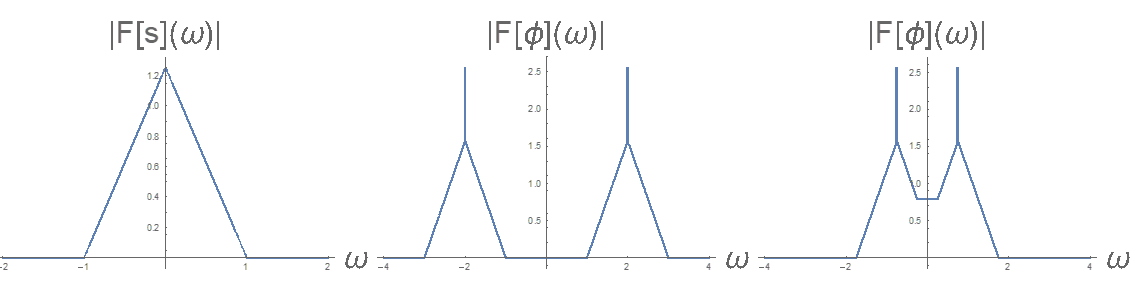
\includegraphics[width=\linewidth]{2016P1Q4.PNG}
    \caption{(Left) $F[s](\omega):=\tilde{s}(\omega)$;  $F[\phi](\omega):=\tilde{s}(\omega)$ for arbitrarily $\Omega=2$ where as long as $\Omega-1>-\Omega+1$ is satisfied (centre) and $\Omega=0.75$ (right).}
\end{figure}
\end{enumerate}
\end{ans}
\begin{qns}[Linear Algebra]\leavevmode
\begin{enumerate}[label=(\alph*)]
\item Given an $n \times n$ matrix $M$ and the identity $I$, show that the matrices $I +M$ and $(I −M)^{−1}$ commute.\hfill\textbf{[4]}
\item Show that the three eigenvalues of a real orthogonal $3\times3$ matrix are $e^{+i\alpha}$, $e^{-i\alpha}$ and $+1$ or $−1$, where $\alpha$ is real.\hfill\textbf{[4]}
\item For a real antisymmetric matrix $A$, the matrix $N$ is defined by
$$N=(I+A)(I-A)^{-1}$$
\begin{enumerate}[label=(\roman*)]
\item Show that $N$ is orthogonal.\hfill\textbf{[3]}
\item Show that eigenvectors of $A$ are also eigenvectors of $N$. What is the relation between the eigenvalues of $A$ and the eigenvalues of $N$?\hfill\textbf{[4]}
\item Show that when $A$ and $N$ are $3\times3$ matrices, $\det N = 1$ and that there exists a direction $x$ in which $Ax = 0$, with $x\neq 0$.\hfill\textbf{[5]}
\end{enumerate}
\end{enumerate}
\end{qns}
\begin{ans}\leavevmode
\begin{enumerate}[label=(\alph*)]
\item Expand and regroup
$$(I+M)(I-M)=I-M+M-M^2=I+M-M-M^2=(I-M)(I+M)$$
Then, multiply $(I-M)^{-1}$ on the left and right for both sides, 
$$(I-M)^{-1}(I+M)(I-M)(I-M)^{-1}=(I-M)^{-1}(I-M)(I+M)(I-M)^{-1}$$
to show $(I-M)^{-1}(I+M)=(I+M)(I-M)^{-1}$.
\item We have $Ae=\lambda e$, then 
$$\lambda|e|^2=e^\dag Ae=(A e)^\dag e=e^\dag A^\dag e=A^{-1}e^\dag e=\lambda^{-1}|e|^2\implies\bigg(\frac{1}{\lambda^*}-\lambda\bigg)|e|^2=0$$
where $A$ is real and orthogonal, so $A^\dag=A^T=A^{-1}$. Since $|e|\neq 0$, we must have $|\lambda|^2=1$.  Then the eigenvalues are either $\pm1$ or come in complex conjugate pairs $e^{\pm i\alpha}$.
\item 
\begin{enumerate}[label=(\roman*)]
\item Before showing $N^TN=I$, we first show $(B^{-1})^T=(B^T)^{-1}$ for any $B$.
$$I=BB^{-1}=(B^{-1})^TB^T\implies (B^T)^{-1}=(B^{-1})^T$$
Then, using $[I+M,(I-M)^{-1}]=0$ from part (a), and that $A^T=-A$:
\begin{align}
    N^TN=[(I+A)(I-A)^{-1}]^T(I+A)(I-A)^{-1}&=[(I-A)^{-1}]^T(I+A)^T(I+A)(I-A)^{-1}\nonumber\\&=[(I-A)^{-1}]^T(I-A)(I+A)(I-A)^{-1}\nonumber\\&=[(I-A)^{-1}]^T(I-A)(I-A)^{-1}(I+A)\nonumber\\&=[(I-A)^{-1}]^T(I+A)\nonumber\\&=(I+A)^{-1}(I+A)=I\nonumber
\end{align}
\item Let $x$ be eigenvectors of $A$ such that $Ax=\lambda x$. Then, $(I-A)^{-1}=(1-\lambda)^{-1}x$, provided $\lambda\neq 1$. This is true since the eigenvalues of an anti-symmetric matrix must be imaginary: We have $Ae=\lambda e$, then 
$$\lambda|e|^2=e^\dag Ae=(A e)^\dag e=e^\dag A^\dag e=e^\dag(-A) e=-\lambda^*|e|^2\implies(\lambda+\lambda^*)|e|^2=0$$
where $A$ is real and anti-symmetric, i.e. $A^\dag=A^T=-A$. So, $\lambda=-\lambda^*$ must be imaginary. Then, 
$$Nx=(I+A)(I-A)^{-1}x=\frac{1+\lambda}{1-\lambda}x$$
$x$ is indeed an eigenvector of $N$ with eigenvalue $\frac{1+\lambda}{1-\lambda}$.
\item Since $A$ is antisymmetric, $A=-A^T$. But 
$$\det A=(-1)^n\det(A^T),\quad\det A=\det A^T$$ 
This means for $n=3$, $\det A=0$. So $\det A=\prod_j\lambda_j=0$, so at least one of the eigenvalues of $A$ must be zero. $\exists$ an eigenvector that $A$ sends to zero. Take $\lambda=0$, then one of the three eigenvalues of $N$ is $+1$. Since $\det N=1$, the other 2 eigenvalues must be complex conjugate pairs.
\end{enumerate}
\end{enumerate}
\end{ans}
\newpage
\begin{qns}[Linear Algebra]\leavevmode
\begin{enumerate}[label=(\alph*)]
\item What does it mean for an $n\times n$ square matrix to be diagonalisable?\hfill\textbf{[2]}
\item Suppose that $A$ is a complex $n\times n$ matrix such that $A^p = 0$ for some positive integer $p$. Show that $A$ has 0 as an eigenvalue. Show that $A$ is not diagonalisable unless $A = 0$.\hfill\textbf{[6]}
\item Let $B$ and $C$ be the matrices
$$B=\begin{pmatrix}4+2\alpha&-2&-2-4\alpha\\3\alpha&-3&9-6\alpha\\2+\alpha&-1&-1-2\alpha\\\end{pmatrix}\text{ and }C=\begin{pmatrix}0&2&6\\3&3&3\\3&1&-3\\\end{pmatrix}$$
By considering the characteristic polynomials of $B$ and $C$, determine whether $B$ and $C$ are diagonalizable.\hfill\textbf{[12]}
\end{enumerate}
\end{qns}
\begin{ans}\leavevmode
\begin{enumerate}[label=(\alph*)]
\item A square matrix $A$ is diagonalizable if there exists a matrix $S$ such that $S^{-1}AS$ is a diagonal matrix. $S$ is constructed from $n$ linearly independent vectors. This is easily found if $A$ possesses $n$ distinct eigenvalues, and thus each eigenvalue will have a separate eigenvector.
\item If $A^p=0$ and $Ae=\lambda e$, then $0=A^pe=\lambda^pe\implies\lambda^p=0\implies\lambda=0$.\\[5pt]
If $A$ were diagonalizable, $\exists S$ such that $S^{-1}AS=\diag(a_1,a_2,...)$. Hence, $(S^{-1}AS)^p=\diag(a_1^p,a_2^p,...)$. But $(S^{-1}AS)^p=S^{-1}A^pS=0$, so $S^{-1}AS=0$ and thus $A=0$.
\item For $B$, we evaluate the determinant along the second row for ease.
\begin{eqnarray}
&&\det(B-\lambda I)\nonumber\\&=&\det\begin{pmatrix}4+2\alpha-\lambda&-2&-2-4\alpha\\3\alpha&-3-\lambda&9-6\alpha\\2+\alpha&-1&-1-2\alpha-\lambda\\\end{pmatrix}\nonumber\\&=&-3\alpha\begin{vmatrix}-2&-2-4\alpha\\-1&-1-2\alpha-\lambda\\\end{vmatrix}+(-3-\lambda)\begin{vmatrix}4+2\alpha-\lambda&-2-4\alpha\\2+\alpha&-1-2\alpha-\lambda\\\end{vmatrix}-(9-6\alpha)\begin{vmatrix}4+2\alpha-\lambda&-2\\2+\alpha&-1\\\end{vmatrix}\nonumber\nonumber\\&=&-3\alpha(2(1+2\alpha+\lambda)-(2+4\alpha))-(3+\lambda)[(2+4\alpha)(2+\alpha)-(4+2\alpha-\lambda)(1+2\alpha+\lambda)]\nonumber\\&&-(9-6\alpha)[2(2+\alpha)-(4+2\alpha-\lambda)]\nonumber\\&=&-\lambda^3\nonumber
\end{eqnarray}
All three eigenvalues are zero. From (b), $B$ is not diagonalizable since it is not the null matrix. For $C$, we evaluate the determinant along the first row.
\begin{eqnarray}
\det(C-\lambda I)&=&\det\begin{pmatrix}-\lambda&2&6\\3&3-\lambda&3\\3&1&-3-\lambda\\\end{pmatrix}\nonumber\\&=&-\lambda\begin{vmatrix}3-\lambda&3\\1&-3-\lambda\\\end{vmatrix}-2\begin{vmatrix}3&3\\3&-3-\lambda\\\end{vmatrix}+6\begin{vmatrix}3&3-\lambda\\3&1\\\end{vmatrix}\nonumber\\&=&-\lambda[-(3-\lambda)^2(3+\lambda)-3]-2[-3(3+\lambda)-9]+6[3-3(3-\lambda)]\nonumber\\&=&36\lambda-\lambda^3\nonumber
\end{eqnarray}
The eigenvalues are $0$ and $\pm 6$. Since there are 3 distinct eigenvalues, from part (a), the matrix is diagonalizable.
\end{enumerate}
\end{ans}
\newpage
\begin{qns}[Cauchy-Riemann]
Consider the mapping $z = f(\zeta)$ such that $G(z) = G(f(\zeta)) =\psi(\zeta)$, where $f$, $G$, $\psi$ are complex functions and $z$, $\zeta$ are complex variables.
\begin{enumerate}[label=(\alph*)]
\item What condition(s) must be satisfied for $\psi(\zeta)$ to be analytic?\hfill\textbf{[3]}
\item Suppose that $\psi(\zeta)=\ln(\zeta+2)$ and $f(\zeta)$ is defined by
\begin{equation}
\frac{df}{d\zeta}=\frac{i}{\sqrt{(\zeta+1)(\zeta-1)}}\tag{*}
\end{equation}
where $\zeta=0$ maps to $z = 0$.
\begin{enumerate}[label=(\roman*)]
\item By integrating, show that the upper half of the $\zeta$ plane maps onto the region $R$ defined by $|\text{Re}(z)|\leq\frac{\pi}{2}$, $\text{Im}(z)\geq 0$. Determine the location of any points in the region $R$ where $G(z)$ is not analytic. How do these relate to points in the $\zeta$ plane? [Hint: $\sin(x + iy) = \sin(x) \cosh(y) + i \cos(x) \sinh(y)$.]\hfill\textbf{[7]}
\item The vector field $\mathbf{u} = (u, v)$ in the $\zeta$ plane is given by $u − iv =\frac{d\psi}{d\zeta}$. How does the magnitude of $\mathbf{u}$ vary across the upper half of the $\zeta$ plane? In what direction is $\mathbf{u}$ oriented?\hfill\textbf{[3]}
\item The vector field $\mathbf{U} = (U, V )$ is defined in the region $R$ of the $z$ plane by $U − iV =\frac{dG}{dz}$. Determine this field and use a sketch to illustrate the orientation of the vector field in this region.\hfill\textbf{[7]}
\end{enumerate}
\end{enumerate}
\end{qns}
\begin{ans}\leavevmode
\begin{enumerate}[label=(\alph*)]
\item A function $\psi=u+iv$ is analytic in $\zeta=a+ib$ if its complex derivative
$$\frac{d\psi}{d\zeta}:=\lim_{\Delta \zeta\rightarrow0}\frac{\psi(\zeta+\Delta\zeta)-\psi(\zeta)}{\Delta\zeta}$$
exists and is independent of the direction of approach of $\Delta\zeta\rightarrow0$ in the complex plane. So, take any two orthogonal directions $\Delta a$ and $i\Delta b$.
$$\lim_{\Delta a\rightarrow0}\frac{\psi(a+\Delta a+ib)-\psi(a+ib)}{\Delta a}=\lim_{\Delta b\rightarrow0}\frac{\psi(a+i(b+\Delta b))-\psi(a+ib)}{i\Delta b}\implies\frac{\partial u}{\partial a}+i\frac{\partial v}{\partial a}=-i\frac{\partial u}{\partial b}+\frac{\partial v}{\partial b}$$
This is the Cauchy-Riemann equations that $\psi(\zeta)$ need to satisfy in order to be analytic.
\item $f$ is a mapping from the $\xi$ plane to the $z$ plane, while $G$ is a mapping  
$$G:~x+iy=z=f(\xi=a+ib)\rightarrow\psi(\xi)$$
\begin{enumerate}[label=(\roman*)]
\item 
We have $df=\frac{d\zeta}{\sqrt{1-\zeta^2}}=\frac{\cos u du}{\sqrt{1-\sin^2u}}\implies f=\sin^{-1}\zeta+C$ where we used $\zeta=\sin u$. As $\sin$ is periodic in its real argument, we must restrict the range of $\sin^{-1}$. Since $\zeta=0\mapsto f(\zeta)=0\implies C=0$. $\zeta$ in terms of $x$ and $y$ is
$$a+ib=\zeta=\sin f(\zeta)=\sin z=\sin x\cosh y+i\cos x\sinh y$$
For Region R, $\frac{\pi}{2}\geq|\text{Re}[z]|=|x|\implies\cos x\geq0$ and together with $\text{Im}[z]=y\geq0\implies\sinh y\geq0$. Hence, $b=\cos x\sinh y\geq0$ which is the upper half-plane of $\xi$.
      \begin{center}
             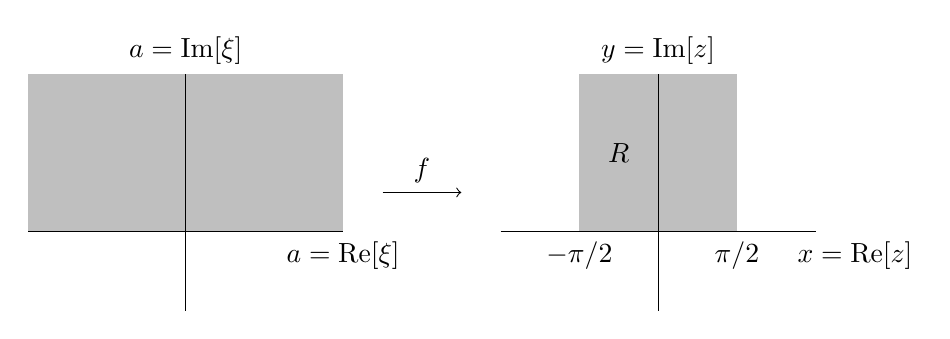
\begin{tikzpicture}
           \fill [black, opacity=0.25] (-2, 2) rectangle (2, 0);
          \draw (-2, 0) -- (2, 0);
          \draw (0,-1) -- (0, 2);
          \node at (2, 0)[below] {$a=\text{Re}[\xi]$};
          \node at (0, 2)[above] {$a=\text{Im}[\xi]$};

          \draw [->] (2.5, 0.5) -- +(1, 0) node [pos=0.5, above] {$f$};
          \begin{scope}[shift={(6, 0)}];
             \fill [black, opacity=0.25] (-1, 2) rectangle (1, 0);
          \draw (-2, 0) -- (2, 0);
          \draw (0, -1) -- (0, 2);
          \node at (-0.5, 1) {$R$};
          \node at (1, 0)[below] {$\pi/2$};
          \node at (-1, 0)[below] {$-\pi/2$};
          \node at (2.5, 0)[below] {$x=\text{Re}[z]$};
          \node at (0, 2)[above] {$y=\text{Im}[z]$};
          \end{scope}
        \end{tikzpicture}
        \end{center}
Now, we want to find the point(s) in R where $G$ is not analytic.
$$G(z)=\psi(\zeta)=\ln(\zeta+2)=\ln(\sin z+2)$$
$G$ is not analytic at either $\sin z=\infty$ or
$$\sin z=\sin x\cosh y+i\cos x\sinh y=-2\implies y=0,~x=\pm\frac{\pi}{2}$$
but $\sin x\cosh0=-2$ has no solution, so only $x=\pm\frac{\pi}{2}$. There is only one solution to $\sin(\pm\frac{\pi}{2})\cosh(y)=-2$, which is $x=-\pi/2$, $y=\cosh^{-1}(2)=\pm\ln(2+\sqrt{2^2-1})=\pm\ln(2+\sqrt{3})$. But $y\geq0$ in region R, so $y=\ln(2+\sqrt{3})$. There is thus only one finite point in region R where $G$ is not analytic: $z=-\frac{\pi}{2}+i\ln(2+\sqrt{3})$.
\item We have
$$u-iv=\frac{d\psi}{d\zeta}=\frac{d}{d\zeta}\ln(\zeta+2)=\frac{1}{\zeta+2}=\frac{a+2-ib}{(a+2)^2+b^2}$$
Hence, $\mathbf{u}=(a+2,b)^T\frac{1}{(a+2)^2+b^2}$ which implies $|\mathbf{u}|=\frac{1}{\sqrt{(a+2)^2+b^2}}$, and $\mathbf{u}$ is directed radially away from the point ($-2$,0) in the $\xi$-plane towards the origin.
\item We have 
$$U-iV=\frac{dG}{dz}=\frac{d}{dz}\ln|2+\sin z|=\frac{\cos z}{2+\sin z}=\frac{\cos x\cosh y-i\sin x\sinh y}{\sin x \cosh y+2+i\cos x\sinh y}$$ This requires
$$U=\text{Re}\bigg[\frac{dG}{dz}\bigg]=\frac{\cos x(2\cosh y+\sin x)}{(2+\sin x\cosh y)^2+\cos^2x\sinh^2y}$$
$$V=\text{Im}\bigg[\frac{dG}{dz}\bigg]=\frac{\sinh y(\cosh y+2\sin x)}{(2+\sin x\cosh y)^2+\cos^2x\sinh^2y}$$
We have $dG=(U-iV)dz=(U+iV)^*(dx+idy)=\mathbf{U}\cdot d\mathbf{l}$. $\mathbf{U}$ is thus orthogonal to the contours of constant $G$, i.e. $G=c\in\mathbb{C}\implies z=\sin^{-1}(e^c-2)$. Plotting $\mathbf{U}$ and $G=c$ in region R ($|\text{Re}[z]|\leq 0.5\pi$, $\text{Im}[z]\geq 0$):
%\begin{center}
%\begin{tikzpicture}
%\begin{axis}[
%xmin = -1.5, xmax = 1.5,
%ymin = 0, ymax = 4,
%zmin = 0, zmax = 1,
%xtick distance = 1,
%ytick distance = 1,
%view = {0}{90},
%xlabel = {$x$},
%ylabel = {$y$},
%colormap/viridis,
%colorbar,
%]
%\addplot3[
%point meta = {sqrt(x^2+y^2)},
%quiver = {
%u = {cos(x)*(2*cosh(y)+sin(x))/((2+sin(x)*cosh(y))^2+(cos(x)*sinh(y))^2)},
%v = {sinh(y)*(cosh(y)+2*sin(x))/((2+sin(x)*cosh(y))^2+(cos(x)*sinh(y))^2)},
%scale arrows = 0.25,
%},
%quiver/colored = {mapped color},
%-stealth,
%domain = -1.5:1.5,
%domain y = 0:4,
%] {0};
%\addplot3[contour gnuplot={number=1,labels=false},thick] 
%				{ln(sin(x+i*y)+2)};
%\end{axis}
%\end{tikzpicture}
%\end{center}
\begin{figure}[H]
    \centering
    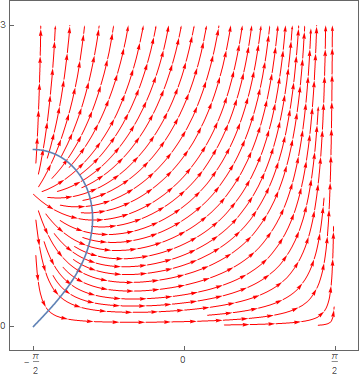
\includegraphics[scale=0.55]{2016P1Q7.png}
    \caption{$\mathbf{U}$ in red and $G=c$ in blue, in region R}
\end{figure}
Important points of the plot: singularity at $(x=-\pi/2,y=\ln(2+\sqrt{3}))$ which has non-zero divergence (This must be true since $\boldsymbol{\nabla}\cdot\mathbf{U}=\frac{\partial U}{\partial x}+\frac{\partial V}{\partial y}=\frac{\partial U}{\partial x}-\frac{\partial U}{\partial x}=0$ everywhere else by Cauchy-Riemann equations since $G$ is analytic $\implies$ $\frac{\partial G}{\partial z}$ is analytic). Near vertical vector field lines at $x=\pm\frac{\pi}{2}$ since $U=0$ for $x=\pm\frac{\pi}{2}$ (numerator has $\cos x$). Near horizontal vector field lines at $y=0$ since $V=0$ for $y=0$ (numerator has $\sinh y$).
\end{enumerate}
\end{enumerate}
\end{ans}
\newpage
\begin{qns}[Series Solution to ODE]\leavevmode
\begin{enumerate}[label=(\alph*)]
\item Define the terms ordinary point and regular singular point for a second order linear differential equation of the form
$$\frac{d^2y}{dx^2}+p(x)\frac{dy}{dx}+q(x)y=0$$
and explain briefly the reason for distinguishing between them.\hfill\textbf{[4]}
\item Let $f(x)$ and $g(x)$ be two differentiable functions on $x\in[a,b]$. Define the Wronskian $W(f, g)(x)$ and show that if $W(f, g)(x_0)\neq 0$ for $x_0\in[a,b]$ then $f$ and $g$ are linearly independent on $[a, b]$.\hfill\textbf{[6]}
\item Find power series solutions of the equation
$$(1-x^2)\frac{d^2y}{dx^2}-x\frac{dy}{dx}+k^2y=0$$
about the point $x = 0$, giving the recurrence relation for the coefficients. Determine the radius of convergence of the solutions about $x = 0$.\hfill\textbf{[10]}
\end{enumerate}
\end{qns}
\begin{ans}\leavevmode
\begin{enumerate}[label=(\alph*)]
\item For the given ordinary differential equation, an ordinary point $x_0$ is where both $p(x)$ and $q(x)$ are analytic at $x=x_0$. A regular singular point $x_1$ is where either $p(x)$ and $q(x)$ are not analytic at $x=x_1$, but both $(x-x_1)p(x)$ and $(x-x_1)^2q(x)$ are analytic at $x=x_1$.\\[5pt]
For a regular singular point, there will always be at least one series expansion of the solution to the differential equation in its neighbourhood. For an ordinary point, there will always exist two linearly independent series solution in its neighbourhood.
\item The Wronksian is defined to be $W(f,g)(x):=fg'-gf'$. For $f$ and $g$ to be linearly dependent in the interval $[a,b]$, there must exist some scalar $\alpha$ such that $f=\alpha g$ everywhere in this interval. Equivalently, $W=0$ everywhere in this interval. Hence, the existence of a single point where $W\neq 0$ is sufficient to guarantee linear independence on every point in the domain within which the functions are differentiable.
\item Since $\frac{-x}{1-x^2}$ and $\frac{k^2}{1-x^2}$ are both analytic at $x=0$, $x=0$ is an ordinary point. We can thus try a series solution of the form $y=\sum_{n=0}^\infty a_nx^n$.
$$\sum_{n=0}^\infty n(n-1)a_nx^{n-2}-\sum_{n=0}^\infty n(n-1)a_nx^n-\sum_{n=0}^\infty na_nx^2+k^2\sum_{n=0}^\infty a_nx^n\implies a_{n+2}=a_n\frac{n^2-k^2}{(n+2)(n+1)}$$
So the series solution is
$$y=\sum_{n=0}^\infty a_nx^n,\quad a_{n+2}=a_n\frac{n^2-k^2}{(n+2)(n=1)}$$
For the series to converge, we require $\lim_{n\rightarrow\infty}|\frac{a_{n+2}}{a_n}||x|^2<1$ $\forall|x|<1$, then the radius of convergence will be
$$R=\lim_{n\rightarrow\infty}\sqrt{\bigg|\frac{a_n}{a_{n+2}}\bigg|}=\lim_{n\rightarrow\infty}\sqrt{\frac{(n+2)(n+1)}{n^2-k^2}}=1$$
\end{enumerate}
\end{ans}
\newpage
\begin{qns}[Variational Principle]\leavevmode
\begin{enumerate}[label=(\alph*)]
\item Suppose that the speed of light $c(y)$ varies continuously through a medium and is a function of the distance from the boundary $y = 0$. Use Fermat’s principle to show that the path $y(x)$ of the light ray is given by the solution of\hfill\textbf{[4]}
$$c(y)y''+c'(y)(1+y'^2)=0$$
\item The curve assumed by a uniform chain, which is suspended between two points $(−a, b)$ and $(a, b)$ minimises the potential energy,
$$\int_{-a}^ay(1+y'^2)^{1/2}dx$$
subject to the constraint that its length remains fixed,
$$\int_{-a}^a(1+y'^2)^{1/2}dx=2L$$
where $L>a$.
\begin{enumerate}[label=(\roman*)]
\item Show that the curve is the catenary
$$y-y_0=k\cosh\frac{x-x_0}{k}$$
where $k$, $x_0$ and $y_0$ are constants.\hfill\textbf{[8]}
\item Find an equation for $k$ and show, using a graphical method, that it has a unique positive solution.\hfill\textbf{[8]}
\end{enumerate}
\end{enumerate}
\end{qns}
\begin{ans}\leavevmode
\begin{enumerate}[label=(\alph*)]
\item Fermat's Principle states that the path adopted by a light ray is one where its time of flight is minimized. The time functional is
$$T[y]=\int\frac{dt}{dl}dl=\int\frac{1}{c(y)}\sqrt{1+y'^2}dx$$
with end points at $x=a,b$. To find stationary $T$, the integral $f$ must satisfy the Euler-Lagrange equation
$$\frac{\partial f}{\partial y}-\frac{d}{dx}\frac{\partial f}{\partial y'}=0$$
where $f(y,y';x)=\frac{1}{c(y)}\sqrt{1+y'^2}$. By Euler-Lagrange,
$$0=-\frac{1}{c^2}c'\sqrt{1+y'^2}-\frac{d}{dx}\frac{1}{c}\frac{y'}{\sqrt{1+y'^2}}\implies c'(1+y'^2)+cy''=0$$
\item
\begin{enumerate}[label=(\roman*)]
\item Extremize
$$F=\int_{-a}^ay(1+y'^2)^{1/2}dx+y_0\bigg(\int_{-a}^a(1+y'^2)^{1/2}dx-2L\bigg)$$
where $y_0$ is the Lagrange multiplier (reason to be made obvious later). But since the integrand $f=(y-y_0)\sqrt{1+y'^2}$ is not explicitly dependent on $x$, then $\frac{\partial f}{\partial x}=0$. By chain rule,
$$\frac{df}{dx}=\frac{\partial f}{\partial x}+\frac{\partial f}{\partial y}y'+\frac{\partial f}{\partial y'}y''=0+y\frac{d}{dx}\frac{\partial f}{\partial y'}+\frac{\partial f}{\partial y'}y''=\frac{d}{dx}y'\frac{\partial f}{\partial y'}$$
where we used the Euler-Lagrange equation. So, $f-y'\frac{\partial f}{\partial y'}$ is a constant, say $k$:
$$k=(y-\lambda)\sqrt{1+y'^2}-\frac{y'(y-y_0)y'}{\sqrt{1+y'^2}}\implies y'=\frac{1}{k}\sqrt{(y-y_0)^2-k^2}$$
We substitute $y-\lambda=k\cosh u$ to get $y-y_0=A\cosh\frac{x-x_0}{k}$.
\item The boundary conditions are $y=b$ for $x=\pm a$, this gives $x_0=0$. Also,
$$2L=\int_{-a}^a\sqrt{1+\sinh^2\frac{x}{k}}dx=2k\sinh\frac{a}{k}$$
We see that graphically, $\sinh(a/k)=L/k$ gives a unique positive solution at $a/k>0$ since $L/a>1$.
\end{enumerate}
\end{enumerate}
\begin{center}
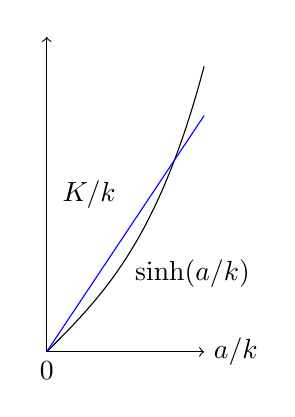
\begin{tikzpicture}
      \draw[->] (0,0) -- (2,0) node[right] {$a/k$};
      \draw[->] (0,0) -- (0,4) node[left] {};
      \draw[domain=0:2,smooth,variable=\x,black] plot ({\x},{sinh(\x)});
      \draw[domain=0:2,smooth,variable=\x,blue] plot ({\x},{1.5*\x});
      \draw (0,0) node[below]{0};
      \draw (1,2) node[left]{$K/k$};
      \draw (1,1) node[right]{$\sinh(a/k)$};
    \end{tikzpicture}
\end{center}
\end{ans}
\begin{qns}[Rayleigh-Ritz Method]\leavevmode
\begin{enumerate}[label=(\alph*)]
\item Let $E_n$ be the eigenvalues of the self-adjoint operator $H$, and $\psi_n$ be the corresponding orthonormal eigenfunctions. Let $F[\phi]$ be the functional
$$F[\phi]=\frac{\int\phi^*H\phi d\tau}{\int \phi^*\phi d\tau}$$
(for finite, non-zero $\int\phi^*\phi d\tau$ ) where $\phi(\tau)$ is a finite arbitrary function and the integration extends from $-\infty$ to $+\infty$.
\begin{enumerate}[label=(\roman*)]
\item If $\psi_n$ is an eigenfunction of $H$, show that\hfill\textbf{[2]}
$$F[\psi_n]=E_n$$
\item Show that if $\phi=\psi_n+\delta\phi$, where $\delta\phi$ is an arbitrary infinitesimal variation, the functional $F[\psi_n]$ is stationary and that
$$(H − F[\psi_n])\phi= 0$$
State any assumptions made.\hfill\textbf{[6]}
\item Show that $F[\phi]$ gives an upper bound to the exact ground state eigenvalue $E_0$ by expanding $\phi$ as
$$\phi=\sum_na_n\psi_n$$
where $\int\phi^*\phi d\tau=\sum_n|a_n|^2$.\hfill\textbf{[2]}
\end{enumerate}
\item Consider a particle of mass $m$ moving in one dimension. For the operator $H =-\frac{\hbar^2}{2m}\frac{d^2}{dx^2}$ for $-a<x<a$, with $H = 0$ elsewhere, the exact ground state eigenvalue $E_0$ is given by
$$E_0=\frac{6\hbar^2}{5ma^2}$$
where $a$ and $\hbar$ are constants. Use the Rayleigh-Ritz method to obtain the lowest upper bound of the value of $E_0$ by choosing a trial function
$$\phi_{trial}(\lambda,x)=
\left\{
        \begin{array}{ll}
      (a^2-x^2)(1+\lambda x^2) & -a\leq x\leq a \\
      0 & |x|>a
        \end{array}
    \right.$$
where $\lambda$ is a real variational parameter.\hfill\textbf{[10]}
\end{enumerate}
[You may assume that the roots to the quadratic equation $13a^4\lambda^2+98a^2\lambda+21$ are approximately $−1/5a^2$ and $−7/a^2$.]
\end{qns}
\newpage
\begin{ans}\leavevmode
\begin{enumerate}[label=(\alph*)]
\item
\begin{enumerate}[label=(\roman*)]
\item Since $H\psi_n=E\psi_n$,
$$F[\psi_n]=\frac{\int_{-\infty}^\infty\psi_n^*H\psi_nd\tau}{\int_{-\infty}^\infty\psi_n^*\psi_n d\tau}=E_n$$
\item With $\phi=\psi_n+\delta\phi$, and discarding higher orders of $\delta\phi$:
\begin{eqnarray}
F[\psi_n+\delta\phi]&=&\frac{\langle\psi_n|H|\psi_n\rangle+\langle\psi_n|H|\delta\phi\rangle+\langle\delta\phi|H|\psi_n\rangle+\langle\delta\phi|H|\delta\phi\rangle}{\langle\psi_n|\psi_n\rangle+\langle\psi_n|\delta\phi\rangle+\langle\delta\phi|\psi_n\rangle+\langle\delta\phi|\delta\phi\rangle}\nonumber\\&=&\frac{E_n+E_n(\langle\psi_n|\delta\phi\rangle+\langle\delta\phi|\psi_n\rangle)+O(\delta\phi^2)}{1+(\langle\psi_n|\delta\phi\rangle+\langle\delta\phi|\psi_n\rangle)+O(\delta\phi^2)}\nonumber\\&=&E_n+O(\delta\phi^2)\nonumber
\end{eqnarray}
We see that there is no first order of $\delta\phi$, hence the functional is stationary, i.e. $\frac{\delta F}{\delta\phi}=0$. Consider the state $$|\Phi\rangle=(H-F[\psi_n])|\phi\rangle=(H-E_n)|\psi_n+\delta\phi\rangle=(E_n-E_n)|\psi_n\rangle+(H-E_n)|\delta\phi\rangle=(H-E_n)|\delta\phi\rangle$$
then the norm of this state is $O(\delta\phi^2)$, which is zero up to the first order. For the norm to be zero, it means the state is zero.
\item The exact ground state is by definition the global minimum eigenvalue. Since the stationary points of $F$ are eigenvalues, $F[\phi]$ must bound $E_0$ from above.
\end{enumerate}
\item With $\phi_{trial}=-\lambda x^4+x^2(-1+a^2\lambda)+a^2\implies\frac{d^2\phi_{trial}}{dx^2}=-12\lambda x^2+2(-1+a^2\lambda)$, then $\int\phi^*\phi dx$ and $\int\phi^*H\phi dx$ respectively gives
$$2\int_0^a\lambda^2x^8+2\lambda x^6(1-a^2\lambda)+x^4(-2\lambda a^2+(-1+a^2\lambda)^2)+2a^2x^2(-1+a^2\lambda)+a^4dx=\frac{16a^5}{315}(\lambda^2a^4+6\lambda a^2+21)$$
\begin{eqnarray}
\int\phi^*H\phi dx&=&-\frac{\hbar^2}{2m}\int\phi^*\frac{d^2}{dx^2}\phi dx\nonumber\\&=&-\frac{\hbar^2}{2m}\int_{-a}^a(-\lambda x^4+x^2(-1+a^2\lambda)+a^2)(-12\lambda x^2+2(-1+a^2\lambda))dx\nonumber\\&=&\frac{\hbar^2}{m}\int_0^a-12\lambda^2x^6+x^4(2\lambda(-1+a^2\lambda)-12\lambda+12a^2\lambda^2)\nonumber\\&&+x^2(12\lambda a^2+2(1-a^2\lambda)(-1+a^2\lambda))-2a^2(-1+a^2\lambda)dx\nonumber\\&=&\frac{4\hbar^2a^3}{105m}(11\lambda^2a^4+14a^2+35)\nonumber
\end{eqnarray}
Then, we must have
$$F[\phi]=\frac{\int\phi^*H\phi dx}{\int\phi^*\phi dx}=\frac{12\hbar^2}{16ma^2}\frac{11\lambda^2a^4+14\lambda a^2+35}{a^4\lambda^2+6\lambda a^2+21}$$
Differentiating with respect to $\lambda$, then
$$0=\frac{\partial F}{\partial\lambda}\implies13\lambda^2a^4+98\lambda a^2+21=0$$
We are given that the roots to this quadratic equation is $-\frac{1}{5a^2}$ and $-\frac{7}{a^2}$, then
$$F[-0.2a^{-2}]=\frac{153}{124}\frac{\hbar^2}{ma^2},\quad F[-7a^{-2}]=\frac{51}{4}\frac{\hbar^2}{ma^2}$$
Our lowest upper bound is the lowest of the two, which is the former. Since $\frac{153\hbar^2}{124ma^2}>E_0=\frac{6\hbar^2}{5ma^2}$, then it is indeed an overestimate of the lowest eigenvalue.
\end{enumerate}
\end{ans}
\newpage
\subsection{Paper 2}
\begin{qns}[Sturm-Liouville]
Consider the Sturm-Liouville system
$$\mathcal{L}y(x)-\lambda\omega(x)y(x)=0,a\leq x\leq b$$
where
$$\mathcal{L}y(x) = −[p(x)y'(x)]' + q(x)y(x)$$
with $\omega(x) > 0$ and $p(x) > 0$ for all $x$ in $[a, b]$. The boundary conditions on y are
$$A_1 y(a) + A_2 y'(a) = 0$$
$$B_1 y(b) + B_2 y'(b) = 0$$
where $A_1$, $A_2$, $B_1$ and $B_2$ are constants and all functions are real.
\begin{enumerate}[label=(\alph*)]
\item Show that with these boundary conditions, $\mathcal{L}$ is self-adjoint.\hfill\textbf{[4]}
\item By considering $y\mathcal{L}y$, or otherwise, show that the eigenvalue $\lambda$ can be written as\hfill\textbf{[4]}
$$\lambda=\frac{\int_a^b[py'^2+qy^2]dx-[pyy']_a^b}{\int_a^b\omega y^2dx}$$
\item Now suppose that $a = 0$ and $b =\ell$, that $p(x) = 1$, $q(x)\geq 0$ and $\omega(x) = 1$ for all x in $[0,\ell]$, and that $A_1 = 1$, $A_2 = 0$, $B_1 = k > 0$ and $B_2 = 1$. Show that the eigenvalues of this Sturm-Liouville system are strictly positive.\hfill\textbf{[4]}
\item Assume further that $q(x) = 0$ and solve the system explicitly. With the aid of a sketch, show that there exist infinitely many eigenvalues $\lambda_1<\lambda_2<...<\lambda_n<...$\hfill\textbf{[6]}
\item Describe the behaviour of $\lambda_n$ as $n\rightarrow\infty$.\hfill\textbf{[2]}
\end{enumerate}
\end{qns}
\begin{ans}\leavevmode
\begin{enumerate}[label=(\alph*)]
\item To be self-adjoint, we require  $\langle u|\mathcal{L}v\rangle=\langle\mathcal{L}u|v\rangle$ for any pair of functions $u$, $v$ that satisfy the given boundary conditions.
$$\langle u|\mathcal{L}v\rangle=\int_a^b-u(pv')'+uqvdx=[-puv']_a^b+\int_a^bu'pv'+uqvdx=[p(u'v-uv')]_a^b+\int_a^b-(pu')'v+uqvdx$$
The boundary condition term is $p(b)(u'(b)v(b)-u(b)v'(b))-p(a)(u'(a)v(a)-u(a)v'(a))$ with each term vanishing on its own, given $A_1u(a)+A_2u'(a)=0\implies A_1u(a)v'(a)+A_2u'(a)v(a)=0$ and $A_1v(a)+A_2v'(a)=0\implies A_1u'(a)v(a)+A_2v'(a)u'(a)$.
\item We have $\langle y|\mathcal{L}y\rangle=\lambda\langle y|y\rangle_\omega$, with the LHS being $$\int_a^b-y(py')'+yqydx=[-pyy']_a^b+\int_a^bpy'^2+qy^2dx\implies\lambda=\frac{\int_a^b[py'^2+qy^2]dx-[pyy']_a^b}{\int_a^b\omega y^2dx}$$
\item The boundary conditions are $y(0)=0$ and $ky(\ell)+y'(\ell)=0$ with $k>0$
$$\lambda=\frac{\int_0^\ell[y'^2+qy^2]dx-[yy']_0^\ell}{\int_0^\ell y^2dx}=\frac{\int_0^\ell[y'^2+qy^2]dx+ky(l)^2}{\int_0^\ell y^2dx}$$
Since the ratio of integrals above is strictly positive, all the eigenvalues will be positive.
\item
With $q(x)=0$, then $\frac{d^2y}{dx^2}=-\lambda y$ with the same boundary conditions. We thus have $y=\sin tx$ such that $\tan(t\ell)=-\frac{t}{k}$. Plot $f(t):=\tan(t\ell)$ and $g(t):=-\frac{t}{k}$, then we can see that there are infinitely many different solutions, each spaced out so that the solutions are never dense on the $t$-axis, and that they increase without limit.
\item As $n\rightarrow\infty$, the intersection point approaches the asymptote at $(2n+1)\frac{\pi}{2}$ and so
$$\lim_{n\rightarrow\infty}\frac{\lambda_n}{(2n+1)0.5\pi}=1$$
\end{enumerate}
\end{ans}
\newpage
\begin{qns}[Laplace's Equation]
Consider the Laplace equation in bipolar coordinates
\begin{equation}
    \frac{\partial^2\Phi}{\partial\sigma^2}+\frac{\partial^2\Phi}{\partial\tau^2}=0\tag{*}
\end{equation}
where $0\leq\sigma < 2\pi$ is a periodic coordinate and $\tau>0$.
\begin{enumerate}[label=(\alph*)]
\item Use separation of variables to show that the general solution of (*), which is continuous and single valued for $\tau>0$, can be written as 
$$\Phi=A_0+B_0\tau+\sum_{n=1}^{+\infty}\bigg\{\bigg[A_n\cosh(n\tau)+B_n\sinh(n\tau)\bigg]\cos(n\sigma)+\bigg[C_n\cosh(n\tau)+D_n\sinh(n\tau)\bigg]\sin(n\sigma)\bigg\}$$
where $A_n$, $B_n$, $C_n$ and $D_n$ are constants.\hfill\textbf{[10]}
\item A line of constant $\tau$ is a circle of radius $1/\sinh\tau$ that can be defined in terms of Cartesian coordinates as
$$y^2+(x-\coth\tau)^2=\frac{1}{\sinh^2\tau}$$
Suppose $\Phi$ satisfies (*) in the region defined by $a<\tau<b$. The inner circle, defined by $\tau= a$, is held at $\Phi=0$ and the outer circle, defined by $\tau=b$, is held at $\Phi=\cos(2\sigma)$. Use separation of variables to find $\Phi$ in the region $a<\tau<b$.\hfill\textbf{[10]}
\end{enumerate}
\end{qns}
\begin{ans}\leavevmode
\begin{enumerate}[label=(\alph*)]
\item Use separation of variables $\Phi(\tau,\sigma)=T(\tau)\Theta(\sigma)$:
$$\frac{1}{\Theta}\frac{d^2\Theta}{d\sigma^2}=-\frac{d^2T}{d\tau^2}=-\lambda^2$$
where $\lambda$ is some constant, then $\Theta(\sigma)=c_1\cos\lambda\sigma+c_2\sin\lambda\sigma$ for $\lambda\neq 0$ and $c_3\sigma+c_4$ for $\lambda=0$. But $\Theta(\sigma+2\pi)=\Theta(\sigma)\implies c_3=c_4=0$ and $\lambda=n\in\mathbb{Z}^+$. Also, $T(\tau)=c_7\tau+c_8$ for $\lambda=0$ and $T(\tau)=c_5\sinh\lambda\tau+c_6\cosh\lambda\tau$ for $\lambda\neq0$. Thus,
$$\Phi(\tau,\sigma)=c_7\tau+c_8+\sum_{n=1}^\infty(c_5\sinh n\tau+c_6\cosh n\tau)(c_1\cos n\sigma+c_2\sin n\sigma)$$
where we identify $c_7=A_0$, $c_8=B_0$, $c_5c_1=B_n$, $c_6c_1=A_n$, $c_2c_6=C_n$, $c_2c_5=D_n$.
\item Plugging into boundary conditions and comparing coefficients for $\Phi(\tau,\sigma)$:
$$0=\Phi(a,\sigma)=A_0+B_0a+\sum_{n=1}^{+\infty}\bigg\{\bigg[A_n\cosh(na)+B_n\sinh(na)\bigg]\cos(n\sigma)+\bigg[C_n\cosh(na)+D_n\sinh(na)\bigg]\sin(n\sigma)\bigg\}$$
which gives $A_0=-B_0a$, $A_n\cosh(na)+B_n\sinh(na)=0$, $C_n\cosh(na)+D_n\sinh(na)=0$ $\forall n\geq1$.
$$\cos2\sigma=\Phi(b,\sigma)=A_0+B_0b+\sum_{n=1}^{+\infty}\bigg\{\bigg[A_n\cosh(nb)+B_n\sinh(nb)\bigg]\cos(n\sigma)+\bigg[C_n\cosh(nb)+D_n\sinh(nb)\bigg]\sin(n\sigma)\bigg\}$$
which gives $A_2\cosh(2b)+B_2\sinh(2b)=1$, $A_0+B_0b=0$, $C_n\cosh(nb)+D_n\sinh(nb)=0$ $\forall n\geq1$ and $A_n\cosh(nb)+B_n\sinh(nb)=0$ $\forall n\geq1$ and $n\neq 2$. This gives $A_n=B_n=0$ $\forall n\neq 2$ and $C_n=D_n=0$ $\forall n$, as well as,
$$\begin{pmatrix}A_2\\B_2\\\end{pmatrix}=\frac{1}{\cosh(2a)\sinh(2b)-\cosh(2b)\sinh(2a)}\begin{pmatrix}\sinh 2b&-\sinh 2a\\-\cosh 2b&\cosh 2a\\\end{pmatrix}\begin{pmatrix}0\\1\\\end{pmatrix}=\frac{1}{\sinh(2(b-a))}\begin{pmatrix}-\sinh(2a)\\\cosh(2a)\\\end{pmatrix}$$
Hence, 
$$\Phi(\tau,\sigma)=\frac{\sinh(2(\tau-a))}{\sinh(2(b-a))}\cos2\sigma$$
\end{enumerate}
\end{ans}
\newpage
\begin{qns}[Green's Functions]
Let $V$ be a region of three-dimensional space with boundary $S$.
\begin{enumerate}[label=(\alph*)]
\item Prove that
$$\int_V(\phi\nabla^2\psi-\psi\nabla^2\phi)dV=\int_S(\phi\mathbf{n}\cdot\boldsymbol{\nabla}\psi-\psi\mathbf{n}\cdot\boldsymbol{\nabla}\phi)dS$$
where $\phi$ and $\psi$  are scalar fields and $\mathbf{n}$ is the outwards directed unit normal to $S$.\hfill\textbf{[3]}
\item Let $\phi$ be a scalar field that tends to zero as $|\mathbf{r}|\rightarrow+\infty$ and satisfies the Poisson equation
$$\nabla^2\phi=-\rho$$
where $\rho(\mathbf{r})$ tends to zero rapidly as $|\mathbf{r}|\rightarrow+\infty$.
\begin{enumerate}[label=(\roman*)]
\item Show that
$$\phi(\mathbf{r})=\int_{\mathbb{R}^3}G(\mathbf{r},\mathbf{\overline{r}})\rho(\mathbf{\overline{r}})d\overline{V}$$
where $G(\mathbf{r},\mathbf{\overline{r}})$ satisfies \hfill\textbf{[3]}
$$\nabla_r^2G(\mathbf{r},\mathbf{\overline{r}})=-\delta^{(3)}(\mathbf{r}-\mathbf{\overline{r}})$$
\item Determine $G(\mathbf{r},\mathbf{\overline{r}})$.\hfill\textbf{[4]}
\item Show that
$$\phi(\mathbf{r})=\frac{e^{-\beta|\mathbf{r}|}-1}{|\mathbf{r}|\beta^2}$$
for the case
$$\rho(\mathbf{r})=-\frac{e^{-\beta|\mathbf{r}|}}{|\mathbf{r}|}$$
where $\beta>0$.\hfill\textbf{[10]}
\end{enumerate}
\end{enumerate}
\end{qns}
\begin{ans}\leavevmode
\begin{enumerate}[label=(\alph*)]
\item Take the Divergence Theorem separately to $\phi\boldsymbol{\nabla}\psi$ and $\psi\boldsymbol{\nabla}\phi$:
$$\int_S\phi\boldsymbol{\nabla}\psi\cdot d\mathbf{S}=\int_V\boldsymbol{\nabla}\cdot(\phi\boldsymbol{\nabla}\psi)dV=\int_V\phi\nabla^2\psi+\boldsymbol{\nabla}\phi\cdot\boldsymbol{\nabla}\psi dV$$
$$\int_S\psi\boldsymbol{\nabla}\phi\cdot d\mathbf{S}=\int_V\boldsymbol{\nabla}\cdot(\psi\boldsymbol{\nabla}\phi)dV=\int_V\psi\nabla^2\phi+\boldsymbol{\nabla}\psi\cdot\boldsymbol{\nabla}\phi dV$$
Now take the difference between the two results:
$$\int_S(\phi\boldsymbol{\nabla}\psi-\psi\boldsymbol{\nabla}\phi)\cdot d\mathbf{S}=\int_V(\phi\nabla^2\psi+\boldsymbol{\nabla}\phi\cdot \boldsymbol{\nabla}\psi-\boldsymbol{\nabla}\psi\cdot\boldsymbol{\nabla}\phi-\psi\nabla^2\phi)dV=\int_V(\phi\nabla^2\psi-\psi\nabla^2\phi)dV$$
\item
\begin{enumerate}[label=(\roman*)]
\item The corresponding $G$ satisfies
$$\nabla_{\mathbf{r}}^2G(\mathbf{r},\mathbf{r'})=-\delta^{(3)}(\mathbf{r}-\mathbf{r'})$$
with $\lim_{|\mathbf{r}|\rightarrow\infty}G(\mathbf{r},\mathbf{r'})=0$. Using result from part (a):
$$\int_S(\phi\boldsymbol{\nabla} G-G\boldsymbol{\nabla}\phi)\cdot d\mathbf{S}=\int_V\phi\nabla^2G-G\nabla^2\phi dV=-\int_V\phi(\mathbf{r})\delta^{(3)}(\mathbf{r}-\mathbf{r'})+G(\mathbf{r},\mathbf{r'})\rho(\mathbf{r})dV$$
where the LHS evaluates to zero due to our boundary conditions. The result follows.
\item Integrate $\nabla_{\mathbf{r}}^2G(\mathbf{r},\mathbf{r'})=-\delta^{(3)}(\mathbf{r}-\mathbf{r'})$ over a sphere of radius $r=|\mathbf{r}-\mathbf{r'}|$ centred on the origin, then
$$\frac{dG}{dr}4\pi r^2=-1\implies G=\frac{1}{4\pi r}+C=\frac{1}{4\pi |\mathbf{r}-\mathbf{r'}|}$$
where $C$ is some constant. But $\lim_{|\mathbf{r}|\rightarrow\infty}G(\mathbf{r},\mathbf{r'})=0$ so $C=0$.
\item From part (b)(i) and (ii), 
\begin{eqnarray}
\phi(\mathbf{r})&=&-\frac{1}{4\pi}\int_{\mathbb{R}^3}\frac{1}{|\mathbf{r}-\mathbf{r'}|}\frac{e^{-\beta|\mathbf{r'}|}}{|\mathbf{r'}|}dV'\nonumber\\&=&\frac{-1}{4\pi}\int_0^{2\pi}d\phi\int_0^\pi\int_0^\infty\frac{r'e^{-\beta r'}}{\sqrt{r^2+r'^2-2rr'\cos\theta}}dr'd\theta'\nonumber\\&=&-\frac{1}{2}\int_0^\infty \frac{e^{-\beta r'}}{r}[\sqrt{r^2+r'^2-2rr'\cos\theta}]_0^\pi dr'\nonumber\\&=&-\frac{1}{2r}\int_0^\infty e^{-\beta r'}(|r+r'|-|r-r'|)dr'\nonumber
\end{eqnarray}
but 
$$|r-r'|=
\left\{
        \begin{array}{ll}
      r-r' & r>r' \\
      -r+r' & r<r'
        \end{array}
    \right.$$
Then, the integral is done piecewise.
\begin{align}
\phi(r)&=-\frac{2}{2r}\bigg(\int_0^rr'e^{-\beta r'}dr'+r\int_r^\infty e^{-\beta r'}dr'\bigg)\nonumber\\&=-\frac{1}{r}\bigg(-\frac{r}{\beta}e^{-\beta r}-\frac{1}{\beta^2}(e^{-\beta r}-1)+\frac{r}{\beta}e^{-\beta r}\bigg)\nonumber\\&=\frac{1}{\beta^2r}(e^{-\beta r}-1)\nonumber
\end{align}
\end{enumerate}
\end{enumerate}
\end{ans}
\begin{qns}[Contour Integration]\leavevmode
\begin{enumerate}[label=(\alph*)]
\item Consider the integral
$$I=\int_C\frac{f(z)}{\sqrt{z}}dz$$
along some contour $C$, where $z=re^{i\theta}$ is complex, $f(z)$ is analytic and nonzero along the real axis, and the branch cut associated with the integrand is taken along the positive real axis.
\begin{enumerate}[label=(\roman*)]
\item Determine the integral $I$ for the contour $C$ given by $r = R$, followed in a clockwise direction from $\theta=\frac{3}{2}\pi$ to $\theta=\frac{1}{2}\pi$, in the limit $R\rightarrow 0$. If f(z) is analytic in the limit $r\rightarrow\infty$, then what constraint needs to be placed on the behaviour of $f(z)$ for the integral to vanish in the limit $R\rightarrow\infty$?\hfill\textbf{[3]}
\item Determine how the value of the integrand just below the branch cut at some $z=x-i\epsilon$ is related to the integrand just above the branch cut at $z = x + i\epsilon$ in the limit $\epsilon\rightarrow0$.\hfill\textbf{[2]}
\end{enumerate}
\item Consider now the function
$$g(z)=\frac{z(z^2+3)}{(z^2+1)(z^2+4)\sqrt{z^2-1}}$$
\begin{enumerate}[label=(\roman*)]
\item Identify the point(s) or region(s) in the complex plane where $g(z)$ is not analytic, stating the nature of the features identified.\hfill\textbf{[3]}
\item Evaluate the integral
$$J=\int_1^\infty g(x)dx$$
using contour integration around a closed contour. Identify contributions from different parts of the contour.\hfill\textbf{[12]}
\end{enumerate}
\end{enumerate}
\end{qns}
\newpage
\begin{ans}\leavevmode
\begin{enumerate}[label=(\alph*)]
\item 
\begin{enumerate}[label=(\roman*)]
\item Parametrize the contour as $z=re^{i\theta}$ with $\theta\in[3\pi/2,\pi/2]$. The integral is:
$$I=\int_C\frac{f(z)}{\sqrt{z}}dz=\int_{3\pi/2}^{\pi/2}\frac{f(Re^{i\theta})}{R^{1/2}e^{i\theta/2}}iRe^{i\theta}d\theta$$
Since $f(z)$ is analytic at $z=0$, $I=O(R^{1/2})\rightarrow 0$ as $R\rightarrow 0$ to vanish as $R\rightarrow\infty$, we require $|f(z)|\rightarrow 0$ faster than $R^{1/2}$.
\item Since $f(z)$ is analytic, only $\sqrt{z}$ changes sign. We have $z^{-1/2}=r^{-1/2}e^{-i\theta/2}$, then $\theta\rightarrow\theta+2\pi$, $z^{-1/2}$ acquires a negative sign ($e^{i\pi}$ phase), i.e. $z^{-1/2}\rightarrow -z^{-1/2}$.
\end{enumerate}
\item 
\begin{enumerate}[label=(\roman*)]
\item $g(z)$ has 
\begin{itemize}
    \item first-order poles at $\pm i$ and $\pm 2i$,
    \item first-order zeros at $0,\pm i\sqrt{3}$,
    \item second-order zero at $\infty$,
    \item branch point singularities at $\pm 1$.
\end{itemize}
We choose branch cuts along $[+1,\infty)$ and $(-\infty,-1]$.
\item We need to choose a contour that avoids the branch point singularities and both branch cuts. A dual keyhole contour of the following form $C=C_1\cup C_2\cup C_3\cup C_4\cup C_5\cup C_6\cup C_7$ would be appropriate:
 \begin{center}
    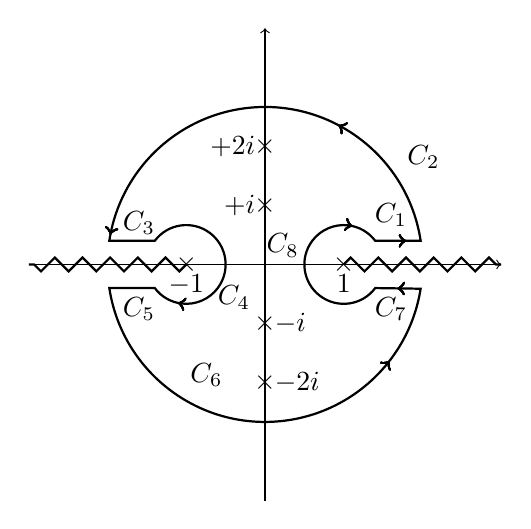
\begin{tikzpicture}
      \draw [->] (-3, 0) -- (3, 0);
      \draw [->] (0, -3) -- (0, 3);
      \draw [thick,decorate, decoration=zigzag] (1, 0) -- (3, 0);
    \draw [thick,decorate, decoration=zigzag] (-1, 0) -- (-3, 0);
      \draw [black, thick, ->-=0.1,->-=0.3, ->-=0.45, ->-=0.75, ->-=0.82, ->-=0.95,->-=0.99] (1.977, 0.3) arc(8.63:171.37:2) node [pos=0.15, anchor = south west] {$C_2$} -- (-1.4, 0.3) arc(143.13:-143.13:0.5)  node [pos=0.7, right] {$C_4$} -- (-1.977, -0.3) arc(188.63:351.13:2)  node [pos=0.3, anchor = south west] {$C_6$}-- (1.4, -0.3) arc(323.13:36.87:0.5) node [pos=0.6, left] {$C_8$}-- cycle;
      \node [circle] at (1,1){};
    \node [below] at (1.6,0.9){$C_1$};
    \node [circle] at (1,-0.5){};
    \node [below] at (1.6,-0.3){$C_7$};
     \node [below] at (-1.6,0.8){$C_3$};
    \node [circle] at (1,-0.5){};
    \node [below] at (-1.6,-0.3){$C_5$};
      \node [circle] at (0, 0) {};
      \node at (-1, 0) {$\times$};
      \node [below] at (-1, 0){$-1$};      
      \node at (1, 0) {$\times$};
      \node [below] at (1, 0){$1$};      
      \node at (0, 0.75) {$\times$};
      \node [left] at (0, 0.75){$+i$};     
      \node at (0, 1.5) {$\times$};
      \node [left] at (0, 1.5){$+2i$};
    \node at (0, -0.75) {$\times$};
      \node [right] at (0, -0.75){$-i$};     
      \node at (0, -1.5) {$\times$};
      \node [right] at (0, -1.5){$-2i$};

    \end{tikzpicture}
  \end{center}
Since $g(z)=O(R^{-2})\rightarrow 0$ as $R\rightarrow\infty$, then the contributions along $\gamma_2$ and $\gamma_2$ vanish. But $g(z)(z\mp1)^{1/2}$ is analytic at $z=\mp 1$ so the contributions from $C_4$ and $C_8$ vanish as well. Thus, we see that
$$\oint_Cg(z)dz\rightarrow \int_{-\infty}^\infty g(x)dx=4J,\text{ as }R\rightarrow\infty$$
The poles enclosed are $\pm i$ and $\pm 2i$ with residues
$$\res_{z=\pm i}g(z)=\lim_{z\rightarrow\pm i}\frac{(z\mp i)z(z^2+3)}{(z^2+1)(z^2+4)\sqrt{z^2-1}}=\frac{\pm i(-1+3)}{\pm 2i(-1+4)\sqrt{-2}}=\frac{1}{3\sqrt{2}i}$$
$$\res_{z=\pm2i}g(z)=\lim_{z\rightarrow\pm i}\frac{(z\mp 2i)z(z^2+3)}{(z^2+1)(z^2+4)\sqrt{z^2-1}}=\frac{\pm 2i(-4+3)}{\pm 4i(-4+1)\sqrt{-4-1}}=\frac{1}{6\sqrt{5}i}$$
By residue theorem, we must have
$$J=\frac{1}{4}\oint_Cg(z)dz=\frac{1}{4}2\pi i\bigg(\frac{2}{3\sqrt{2}i}+\frac{2}{6\sqrt{5}i}\bigg)=\frac{\pi}{3\sqrt{2}}+\frac{\pi}{6\sqrt{5}}$$
\end{enumerate}
\end{enumerate}
\end{ans}
\newpage
\begin{qns}[Transform Methods]
The Fourier transform of $y(t)$ is given by
\begin{equation}
    \tilde{y}(\omega)=\frac{-\omega\tilde{f}(\omega)}{\omega^3-i\omega^2+4\omega-4i}\tag{*}
\end{equation}
where $\tilde{f}(\omega)$ is the Fourier transform of the function $f(t)$, and both $y(t)$ and $f(t)$ vanish as $t\rightarrow\pm\infty$.
\begin{enumerate}[label=(\alph*)]
\item Determine the third order differential equation that governs $y(t)$.\hfill\textbf{[3]}
\item Find $f(t)$, valid for all $t$, for the case\hfill\textbf{[5]}
\begin{equation}
    \tilde{f}(\omega)=\frac{-i}{\omega-i}\tag{\dag}
\end{equation}
\item Substitute (\dag) into (*) and use an inverse Fourier transform to determine $y(t)$, valid for all $t$. Sketch the behaviour of $y(t)$.\hfill\textbf{[12]}
\end{enumerate}
\end{qns}
\begin{ans}\leavevmode
\begin{enumerate}[label=(\alph*)]
\item Rearrange (*):
$$\omega^3\tilde{y}(\omega)-i\omega^2\tilde{y}(\omega)+4\omega \tilde{y}(\omega)-4i\tilde{y}(\omega)=-\omega\tilde{f}(\omega)$$
Since $y(t)$ and $f(t)$ vanish as $|t|\rightarrow\infty$, then further assume $\frac{dy}{dt}$ and $\frac{d^2y}{dt^2}$ have similar asymptotic behaviours, then taking the inverse Fourier transform of (*) gives $\tilde{y}^{(n)}=(i\omega)^n\tilde{y}$. So multiply $-i$ across.
$$i\omega\tilde{f}(\omega)=-i\omega^3\tilde{y}(\omega)-\omega^2\tilde{y}(\omega)-4i\omega \tilde{y}(\omega)-4\tilde{y}(\omega)=\tilde{y}'''+\tilde{y}''-4\tilde{y}'-4\tilde{y}$$
Perform inverse FT, the ODE is
$$\frac{df}{dt}=y'''+y''-4y'-4y$$
\item The inverse Fourier transform is
$$f(t)=\frac{1}{2\pi}\int_{-\infty}^\infty\frac{-i}{\omega-i}e^{i\omega t}d\omega$$
The integrand has first order pole at $\omega=i$ with residue
$$\res_{\omega=i}\frac{-i}{\omega-i}\frac{e^{i\omega t}}{2\pi}=\frac{-ie^{-t}}{2\pi}$$
For $t>0$, we close the contour in upper half-plane to invoke Jordan's Lemma:
$$\oint_{C:=C_R\cup C_0}\frac{-i}{\omega-i}e^{i\omega t}d\omega=\int_{C_R}\frac{-i}{\omega-i}e^{i\omega t}d\omega+\int_{-R}^R\frac{-i}{\omega-i}e^{i\omega t}d\omega\rightarrow 0+2\pi f(t>0)$$
\begin{center}
    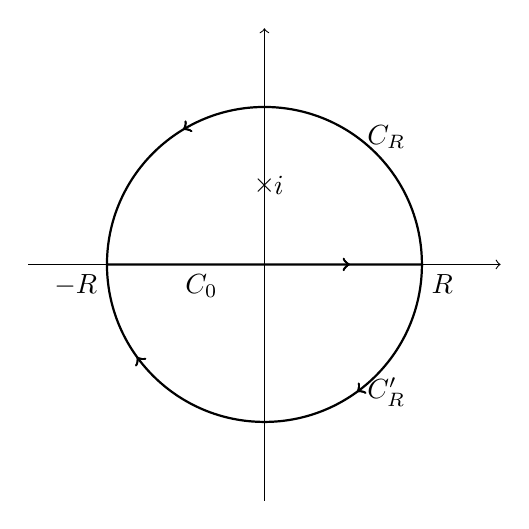
\begin{tikzpicture}
      \draw [->] (-3, 0) -- (3, 0);
      \draw [->] (0, -3) -- (0, 3);

     \draw [black, thick, ->-=0.3, ->-=0.8] (-2, 0) -- (2, 0) node [pos=0.3, below] {$C_0$} arc(0:180:2) node [pos=0.3, right] {$C_R$};
      \draw [black, thick, ->-=0.3, ->-=0.8] (2, 0) arc(0:-180:2) node [pos=0.3, right] {$C_R'$};

      \node [anchor = north east] at (-2, 0) {$-R$};
      \node [anchor = north west] at (2, 0) {$R$};
      \node [circle] at (-2, 0) {};
      \node [circle] at (2, 0) {};

      \node at (0, 1) {$\times$};
      \node [right] at (0, 1) {$i$};

    \end{tikzpicture}
  \end{center}
  By residue theorem, we have
  $$\oint_{C:=C_R\cup C_0}\frac{-i}{\omega-i}e^{i\omega t}d\omega=2\pi i\frac{-ie^{-t}}{2\pi}=e^{-t}$$
  For $t<0$, we close the lower half-plane and again invoke Jordan's Lemma:
  $$\oint_{C':=C_R'\cup C_0}\frac{-i}{\omega-i}e^{i\omega t}d\omega=\int_{C_R'}\frac{-i}{\omega-i}e^{i\omega t}d\omega+\int_{-R}^R\frac{-i}{\omega-i}e^{i\omega t}d\omega\rightarrow 0+2\pi f(t<0)$$
  But no pole is enclosed so by residue theorem, $f(t<0)=0$. Similarly, for $t=0$, we just have
  $$f(t)=\frac{1}{2\pi}\int_{-\infty}^\infty-\frac{i}{\omega -i}d\omega=0$$
  Hence, the solution is
  $$f(t)=
\left\{
        \begin{array}{ll}
      e^{-t} & t>0 \\
      0 & t\leq0
        \end{array}
    \right.$$
\item (*) becomes
$$\tilde{y}(\omega)=\frac{-\omega}{\omega^3-i\omega^2+4\omega-4i}\frac{-i}{\omega-i}=\frac{\omega i}{(\omega-i)^2(\omega+2i)(\omega-2i)}$$
which has a second order pole at $\omega=i$ and simple poles at $\omega=\pm 2i$. By inverse Fourier transform, the solution would be
$$y(t)=\frac{1}{2\pi}\int_{-\infty}^\infty\frac{\omega i}{(\omega-i)^2(\omega+2i)(\omega-2i)}e^{i\omega t}d\omega$$
Repeat a similar computation using the same contour:
\begin{center}
    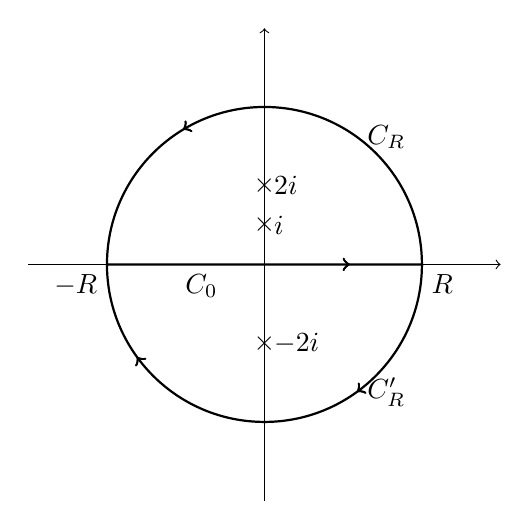
\begin{tikzpicture}
      \draw [->] (-3, 0) -- (3, 0);
      \draw [->] (0, -3) -- (0, 3);

     \draw [black, thick, ->-=0.3, ->-=0.8] (-2, 0) -- (2, 0) node [pos=0.3, below] {$C_0$} arc(0:180:2) node [pos=0.3, right] {$C_R$};
      \draw [black, thick, ->-=0.3, ->-=0.8] (2, 0) arc(0:-180:2) node [pos=0.3, right] {$C_R'$};

      \node [anchor = north east] at (-2, 0) {$-R$};
      \node [anchor = north west] at (2, 0) {$R$};
      \node [circle] at (-2, 0) {};
      \node [circle] at (2, 0) {};

      \node at (0, 1) {$\times$};
      \node [right] at (0, 1) {$2i$};
        \node at (0, -1) {$\times$};
      \node [right] at (0, -1) {$-2i$};
      \node at (0, 0.5) {$\times$};
      \node [right] at (0, 0.5) {$i$};
    \end{tikzpicture}
  \end{center}
The residues at the three poles are
\begin{align}
\res_{\omega=i}\frac{\omega i}{(\omega-i)^2(\omega+2i)(\omega-2i)}\frac{e^{i\omega t}}{2\pi}&=\frac{1}{2\pi}\lim_{\omega\rightarrow i}\frac{d}{d\omega}\frac{\omega i}{(\omega+2i)(\omega-2i)}e^{i\omega t}\nonumber\\&=\frac{1}{2\pi}\lim_{\omega\rightarrow i}\frac{i(1+i\omega t)e^{i\omega t}(\omega^2+4)-i\omega e^{i\omega t}2\omega}{(\omega^2+4)^2}\nonumber\\&=\frac{3i(1-t)e^{-t}+2ie^{-t}}{18\pi}\nonumber\\&=\frac{5-3t}{18\pi}ie^{-t}\nonumber
\end{align}
$$\res_{\omega=\pm 2i}\frac{\omega i}{(\omega-i)^2(\omega+2i)(\omega-2i)}\frac{e^{i\omega t}}{2\pi}=\frac{1}{2\pi}\lim_{\omega\rightarrow\pm 2i}\frac{i\omega e^{i\omega t}}{(\omega-i)^2(\omega\pm 2i)}$$
which gives $\frac{-i}{4\pi}e^{-2t}$ for $\omega=2i$ and $\frac{-i}{36\pi}e^{2t}$ for $\omega=-2i$. For $t>0$, again we close the upper half-plane in order to invoke Jordan's Lemma:
\begin{eqnarray}
&&\oint_{C:=C_R\cup C_0}\frac{\omega i}{(\omega-i)^2(\omega+2i)(\omega-2i)}e^{i\omega t}d\omega\nonumber\\&=&\int_{C_R}\frac{\omega i}{(\omega-i)^2(\omega+2i)(\omega-2i)}e^{i\omega t}d\omega+\int_{-R}^R\frac{\omega i}{(\omega-i)^2(\omega+2i)(\omega-2i)}e^{i\omega t}d\omega\nonumber\\&\rightarrow 0&+2\pi y(t>0)\nonumber
\end{eqnarray}
The two poles enclosed are $2i$ and $i$, so by residue theorem,
$$y(t>0)=\frac{1}{2\pi}\oint_{C:=C_R\cup C_0}\frac{\omega i}{(\omega-i)^2(\omega+2i)(\omega-2i)}e^{i\omega t}d\omega=2\pi i\bigg(\frac{-i}{4\pi}e^{-2t}+\frac{5-3t}{18\pi}ie^{-t}\bigg)$$
Again, for $t<0$, we close the lower half-plane and invoke Jordan's Lemma:
\begin{eqnarray}
&&\oint_{C':=C_R'\cup C_0}\frac{\omega i}{(\omega-i)^2(\omega+2i)(\omega-2i)}e^{i\omega t}d\omega\nonumber\\&=&\int_{C_R}\frac{\omega i}{(\omega-i)^2(\omega+2i)(\omega-2i)}e^{i\omega t}d\omega+\int_{-R}^R\frac{\omega i}{(\omega-i)^2(\omega+2i)(\omega-2i)}e^{i\omega t}d\omega\nonumber\\&\rightarrow 0&+2\pi y(t<0)\nonumber
\end{eqnarray}
again by residue theorem,
$$\frac{1}{2\pi}\oint_{C':=C_R'\cup C_0}\frac{\omega i}{(\omega-i)^2(\omega+2i)(\omega-2i)}e^{i\omega t}d\omega=2\pi i\bigg(\frac{-i}{36\pi}e^{2t}\bigg)$$
The solution is thus
  $$y(t)=
\left\{
        \begin{array}{ll}
      -\frac{1}{18}e^{2t} & t<0 \\
      \frac{1}{2}e^{-2t}+\frac{3t-5}{9}e^{-t} & t>0
        \end{array}
    \right.$$
Since $f$ is discontinuous at $t=0$ and $\dot{f}=\infty$ at $t=0$, we must have $\ddot{y}$ to have a unit discontinuity while both $y$ and $\dot{y}$ are continuous.
\begin{center}
\begin{tikzpicture}
      \draw[->] (-3,0) -- (3,0) node[right] {$t$};
      \draw[->] (0,0) -- (0,-1) node[below] {$y(t)$};
      \draw[domain=-3:0,smooth,variable=\x,black] plot ({\x},{(-10/18)*exp(2*\x)});
      \draw[domain=0:3,smooth,variable=\x,black] plot ({\x},{5*exp(-2*\x)+(3*\x-5)*10*exp(-\x)/9}); %scale by factor of 10
      \draw (0,0) node[above]{0};
    \end{tikzpicture}
\end{center}
\end{enumerate}
\end{ans}
\begin{qns}[Tensors]\leavevmode
\begin{enumerate}[label=(\alph*)]
\item Define an order two tensor.\hfill\textbf{[2]}
\item The quantity $C_{ij}$ has the property that for every order two tensor $A_{ij}$, the quantity $C_{ij}A_{ij}$ is a scalar. Prove that $C_{ij}$ is necessarily an order two tensor.\hfill\textbf{[4]}
\item Show that if a tensor $T_{ij}$ is invariant under a rotation of $\pi/2$ about the $x_3$-axis then it has the form
$$\begin{pmatrix}\alpha&\omega&0\\-\omega&\alpha&0\\0&0&\beta\\\end{pmatrix}$$
Also show that $T_{ij}$ is invariant under a general rotation about the $x_3$-axis.\hfill\textbf{[6]}
\item The inertia tensor about the origin of a rigid body occupying volume $V$ with mass density $\rho(\mathbf{x})$ is defined as
$$I_{ij}=\int_V\rho(\mathbf{x})(x_kx_k\delta_{ij}-x_ix_j)dV$$
The rigid body B has uniform density $\rho$ and occupies the cylinder
$$\{(x_1,x_2,x_3):-2\leq x_3\leq 2,x_1^2+x_2^2\leq 1\}$$
Show that the inertia tensor of B about the origin is diagonal in the $(x_1, x_2, x_3)$ coordinate system and calculate its diagonal elements.\hfill\textbf{[8]}
\end{enumerate}
\end{qns}
\newpage
\begin{ans}\leavevmode
\begin{enumerate}[label=(\alph*)]
\item An order-2 tensor has components $D_{ij}$ such that under any orthogonal transformation of the coordinates, it remains invariant. Hence, the components must transform as
$$D_{ij}'=L_{i\alpha}L_{j\beta}D_{\alpha\beta}$$
where $L$ is the orthogonal transformation matrix.
\item $(C_{ij}A_{ij})'=C_{ij}'A_{ij}'=C_{ij}'L_{i\alpha}L_{j\beta}A_{\alpha\beta}$.
$$C_{ij}'L_{i\alpha}L_{j\beta}=C_{\alpha\beta}\implies C_{ij}'\delta_{ip}\delta_{jq}=L_{p\alpha}L_{q\beta}C_{\alpha\beta}\implies C'_{pq}=L_{p\alpha}L_{q\beta}C_{\alpha\beta}$$
Indeed, a rank-two tensor.
\item Assume $T$ is three-dimensional. Let's rotate around $x_1$-$x_2$ plane by $\frac{\pi}{2}$:
$$L=\begin{pmatrix}0&1&0\\-1&0&0\\0&0&1\\\end{pmatrix}$$
Then, 
$$T_{ij}'=L_{ip}T_{pq}L_{jq}=(LTL^T)_{ij}=\begin{pmatrix}T_{22}&-T_{21}&T_{23}\\-T_{12}&T_{11}&-T_{13}\\T_{32}&-T_{31}&T_{33}\\\end{pmatrix}$$
Then, for $T'=T$, we have $T_{11}=T_{22}$ with $T_{33}$ unconstrained. Call the former $\alpha$ and latter $\beta$. $-T_{21}=T_{12}$, $-T_{12}=T_{21}$, and must be the same value. Call this $\omega$. Now, $T_{23}=T_{13}$, $-T_{13}=T_{23}$, $T_{32}=T_{31}$, $-T_{31}=T_{32}$, all zero.\\[5pt]
Now apply generic rotation about the $x_3$-axis to $T_{ij}$, i.e show
$$L'TL'T=T,\quad L'=\begin{pmatrix}\cos\theta &\sin\theta&0\\-\sin\theta&\cos\theta&0\\0&0&1\\\end{pmatrix}$$
\item The cylindrical axis is $x_3$. The system is symmetric under arbitrary rotations in the $x_1$-$x_2$ plane, hence $I_{ij}$ has the form $T_{ij}$ in part (c). We proceed to compute the individual elements:
$$I_{12}-I_{21}=\rho\int_V(x_kx_k(\delta_{12}-\delta_{21})-x_1x_2+x_2x_1)dV=0$$
but $T_{12}-T_{21}=2\omega$, hence the off-diagonal elements of $I_{ij}$ must be zero.
$$I_{11}=I_{22}=\int_{-2}^2\int_0^1\int_{-\pi}^\pi\rho(r^2+x_3^2-(r\cos\theta)^2)r d\theta dr dx_3=\frac{19}{3}\pi\rho$$
$$I_{33}=\rho\int_{-2}^2\int_0^1\int_{-\pi}^\pi r^2rd\theta dr dx_3=2\pi\rho$$
Thus,
$$I=\pi\rho\begin{pmatrix}19/3&0&0\\0&19/3&0\\0&0&2\\\end{pmatrix}$$
\end{enumerate}
\end{ans}
\newpage
\begin{qns}[Normal Coordinates]
A mass $m_1$ is suspended from the origin by a spring with spring constant $k_1$. A second mass $m_2$ is suspended from the first by a spring with spring constant $k_2$. Both springs are of a type that has zero length when not extended. The motion of the masses is restricted to the $(x, y)$ plane such that m1 is located at $(X_1(t), Y_1(t))$ and $m_2$ is located at $(X_2(t), Y_2(t))$. Gravity acts in the $−y$ direction.
\begin{enumerate}[label=(\alph*)]
\item Write down the Lagrangian for the system and hence use the Euler-Lagrange equation to determine the equations of motion for the system.\hfill\textbf{[6]}
\item Determine the equilibrium position $(\hat{X}_1,\hat{Y}_1,\hat{X}_2,\hat{Y}_2)$. Suppose the setup is altered so that $X_2(t)=\hat{X}_2$. Show that small perturbations $(x_1(t),y_1(t),y_2(t))$ about the equilibrium are governed by\hfill\textbf{[3]}
$$\begin{pmatrix}m_1&0&0\\0&m_1&0\\0&0&m_2\\\end{pmatrix}\begin{pmatrix}\ddot{x}_1\\\dot{y}_1\\\dot{y}_2\\\end{pmatrix}+\begin{pmatrix}k_1+k_2&0&0\\0&k_1+k_2&-k_2\\0&-k_2&k_2\\\end{pmatrix}\begin{pmatrix}x_1\\y_1\\y_2\\\end{pmatrix}=\begin{pmatrix}0\\0\\0\\\end{pmatrix}$$
\item Determine the frequency and structure of each of the modes for the case $m_1=m_2=m$ and $k_1=k_2=k$.\hfill\textbf{[11]}
\end{enumerate}
\end{qns}
\begin{ans}\leavevmode
\begin{enumerate}[label=(\alph*)]
\item The Lagrangian for the system is
$$\mathcal{L}=\frac{1}{2}m_1(\dot{X}_1^2+\dot{Y}_1^2)+\frac{1}{2}m_2(\dot{X}_2^2+\dot{Y}_2^2)-\frac{1}{2}k_1(X_1^2+Y_1^2)-\frac{1}{2}k_2((X_1-X_2)^2+(Y_1-Y_2)^2)+m_1gY_1+m_2gY_2$$
where we define the zero-position for the GPE is at $y=0$. When the Lagrangian is extremized, it satisfies the Euler-Lagrange equations for each independent variable $q_i$:
$$\frac{d}{dt}\frac{\partial\mathcal{L}}{\partial\dot{q}_i}=\frac{\partial\mathcal{L}}{\partial q_i}$$
Then, the equations of motion are
$$m_1\ddot{X}_1=-k_1X_1-k_2(X_1-X_2)$$
$$m_1\ddot{Y}_1=-k_1Y_1-k_2(Y_1-Y_2)+m_1g$$
$$m_2\ddot{X}_2=-k_2(X_2-X_1)$$
$$m_2\ddot{Y}_2=-k_2(Y_2-Y_1)+m_2g$$
\item Equilibrium position is attained when the acceleration is zero. So, writing in matrix form:
$$\begin{pmatrix}-k_1-k_2&k_2\\k_2&-k_1\\\end{pmatrix}\begin{pmatrix}\hat{X}_1\\\hat{X}_2\\\end{pmatrix}=\begin{pmatrix}0\\0\\\end{pmatrix}\implies\hat{X}_1=\hat{X}_2=0$$
$$\begin{pmatrix}-k_1-k_2&k_2\\k_2&-k_1\\\end{pmatrix}\begin{pmatrix}\hat{Y}_1\\\hat{Y}_2\\\end{pmatrix}=\begin{pmatrix}m_1g\\m_2g\\\end{pmatrix}\implies\hat{Y}_1=-\frac{(m_1+m_2)g}{k_1},\quad \hat{Y}_2=-\frac{(m_1+m_2)g}{k_1}-\frac{m_2g}{k_2}$$
Now we alter the setup such that $x_2(t)=X_2-\hat{X}_2=0$, $x_1(t)=X_1-\hat{X}_1$, $y_i(t)=Y_i-\hat{Y}_i$ for $i=1,2$, then from the equations of motion, we obtained the desired relation.
\item Set $m_1=m_2=m$, $k_1=k_2=k$, and seek solutions of the form $(x_1,y_1,y_2)^T=(a,b,c)^Te^{i\omega t}$, then this is equivalent to solving
$$0=\det\begin{pmatrix}2k-m\omega^2&0&0\\0&2k-m\omega^2&-k\\0&-k&k-m\omega^2\\\end{pmatrix}=(k-2m\omega^2)((2k-m\omega^2)(k-m\omega^2)-k^2)$$
Then we have $\omega_0^2=\frac{2k}{m}$, $\omega_\pm^2=\frac{k}{2m}(3\pm\sqrt{5})$. By inspection, the corresponding eigenvector for $\omega_0$ is $(1,0,0)^T$. And we can work out the remaining eigenvectors to be $(0,1,3\pm\sqrt{5})^T$. The modes thus look like $(1,0,0)^Te^{i\sqrt{2k/m}t}$ and $(0,1,3\pm\sqrt{5})^Te^{i\sqrt{k(3\pm\sqrt{5})/m}t}$.
\end{enumerate}
\end{ans}
\newpage
\begin{qns}[Group Theory]\leavevmode
\begin{enumerate}[label=(\alph*)]
\item Given a finite group $G$ of order $|G|$ and a normal subgroup $N$ of order $|N|$, define the quotient group $G/N$ and show that it is indeed a group. State Lagrange’s theorem relating the order of a group and those of its subgroups.\hfill\textbf{[2]}
\item Show that the Pauli matrices together with the identity matrix
$$\sigma_x=\begin{pmatrix}0&1\\1&0\\\end{pmatrix},\quad\sigma_y=\begin{pmatrix}0&-i\\i&0\\\end{pmatrix},\quad\sigma_z=\begin{pmatrix}1&0\\0&-1\\\end{pmatrix},\quad I=\begin{pmatrix}1&0\\0&1\\\end{pmatrix}$$
do not constitute a group under matrix multiplication. Show that these matrices can be multiplied by $\pm 1$ and $\pm i$, to generate a set of 16 matrices, which meet the conditions to form a group.\hfill\textbf{[9]}
\item Prove that in any group, an element and its inverse have the same order.\hfill\textbf{[9]}
\end{enumerate}
\end{qns}
\begin{ans}\leavevmode
\begin{enumerate}[label=(\alph*)]
\item $G/N$ is the set of left cosets of $N\leq G$, i.e.
$$gN=\{g\in G|~g'=g*n\text{ for some }n\in N\}$$
Check group axioms:
\begin{itemize}
    \item closure: For $g_1N,g_2N\in G/N$, $g_1Ng_2N=g_1g_2N\in G/N$ since $g_1,g_2\in G\implies g_1,g_2\in G$.
    \item associativity: inherit from parent group $G$.
    \item identity: $eN\in G/N$.
    \item inverse: $g^{-1}NgN=eN\implies g^{-1}N\in G/N$.
\end{itemize}
Lagrange's theorem states that for $H\leq G$, then $\frac{|G|}{|H|}\in\mathbb{N}$.
\item Take for instance,
$$\begin{pmatrix}0&1\\1&0\\\end{pmatrix}\begin{pmatrix}1&0\\0&-1\\\end{pmatrix}=\begin{pmatrix}0&-1\\1&0\\\end{pmatrix}\notin\{\sigma_x,\sigma_y,\sigma_z,\Id\}$$
The set $\{\sigma_x,\sigma_y,\sigma_z,\Id\}$ is not closed. Essentially,
$$\sigma_x\sigma_y=i\sigma_z=-\sigma_y\sigma_x,\quad\sigma_y\sigma_z=i\sigma_x=-\sigma_z\sigma_y,\quad \sigma_z\sigma_x=i\sigma_y=-\sigma_x\sigma_z$$
Any arbitrary element can be written as $(-1)^n\sigma_x^a\sigma_y^b\sigma_z^c$. So, check closure again:
$$(-1)^n\sigma_x^a\sigma_y^b\sigma_z^c(-1)^p\sigma_x^\alpha\sigma_y^\beta\sigma_z^\gamma=(-1)^{n+p}\sigma_x^{a+\alpha}\sigma_y^{b
+\beta}\sigma_z^{c+\gamma}$$
The powers are only meaningful if they are either 0 or 1 since $\sigma_p^2=\Id$ $\forall p=x,y,z$. So the new set is closed. The set contains the identity $\Id$ (raise to zero power for all). The binary operation (matrix multiplication) is associative. The inverse is $(-1)^n\sigma_x^{-a}\sigma_y^{-b}\sigma_z^{-c}$ if $a,b,c\neq 0$ and $(-1)^n\sigma_x^a\sigma_y^b\sigma_z^c$ if only one of $a,b,c$ is not zero. All the group axioms are satisfied, so this new set of $2^4=16$ distinct elements is a group.
\item Let $g,h\in G$ such that $hg=e$ where $e$ is the identity in $G$. Let $\ord(g)=p$, $\ord(h)=q$, i.e. $g^p=e=h^q$, then 
$$e=e^p=(gh)^p=g^ph^p=eh^p$$
so $q$ is a factor of $q$. Similarly, we can show $p$ is a factor of $q$. Hence, $q=p$ and thus $g$ and $h=g^{-1}$ has the same order.

\end{enumerate}
\end{ans}
\newpage
\begin{qns}[Group Theory]\leavevmode
\begin{enumerate}[label=(\alph*)]
\item Let $G$ be a finite subgroup. The centre $Z(G)$ of $G$ is the set of elements $z\in G$ that commute with every element $g\in G$, that is to say
$$Z(G) = \{z\in G : gz = zg, \forall g\in G\}$$
Prove that if $H$ is a normal subgroup of $G$ with order $|H| = 2$, then $H\subseteq Z(G)$.\hfill\textbf{[7]}
\item Define a homomorphism between two groups $H$ and $G$. Define the kernel of a homomorphism.

\hfill\textbf{[3]}
\item Suppose that $G$ is a group of order $|G| = 21$. Show that every proper subgroup of $G$ is cyclic.

\hfill\textbf{[10]}
\end{enumerate}
\end{qns}
\begin{ans}\leavevmode
\begin{enumerate}[label=(\alph*)]
\item A normal subgroup is the union of complete conjugacy classes. The conjugacy classes are
$$\ccl(g)=\{g'\in G|~g'=lgl^{-1}\text{ for some }l\in G\}$$
Elements that commute with all other elements are thus in a class of their own, as $lgl^{-1}=ll^{-1}g=g$ $\forall l\in G$. The identity trivially commutes with every element in the group. The  centre thus consists of complete conjugacy classes, so $Z(G)\lhd G$.\\[5pt]
Since $H\lhd G$ and $|H|=2$. Let $H=\{e,h\}$, then $h$ is a conjugacy class of its own. 
$$lhl^{-1}=h~\forall l\in G\implies hl=lh\implies h\in Z\implies H\subseteq Z(G)$$
\item If $H$ and $G$ are groups, then a function $\Phi:~H\rightarrow G$ is a group homomorphism, if $\forall a,b\in H$, $\Phi(a\cdot_Hb)=\Phi(a)\cdot_G\Phi(b)$. The kernel of $\Phi$ is
$$\Ker\Phi=\{h\in H|~\Phi(h)=e_G\text{ for some }h\in H\}$$
\item Consider $H\leq G$, the cosets of $H$ in $G$ are $g_iH$ $\forall g_i\in G$. $H\leq G\implies e\in H\implies g_i\in g_iH$, so each element in $G$ is in at least one coset. Now suppose two cosets generated by distinct $g_i,g_j\in G$ share an element, then for some $h_i,h_j\in H$,
$$g_ih_i=g_jh_j\implies g_ih_ih_j^{-1}=g_j\implies g_jH=g_ih_ih_j^{-1}H=g_ih_iH=g_iH$$
The cosets are either disjoint or identical, so every element $g_i\in G$ is in at most one coset. The cosets thus partition the group into blocks of size equal to the size of the generating subgroup. The order of the group is thus the order of the subgroups times the number of cosets.\\[5pt]
Consider the generator of any $g\in G$, $\langle g\rangle=\{g,g^2,g^3,\dots,e\}$ has $\ord(g)$ elements and is a group since it
\begin{itemize}
    \item is closed, i.e. $g^pg^q=g^{r}$ where $r=p+q$ mod $\ord(g)$.
    \item inherit associativity from $G$.
    \item contains the identity.
    \item for $g^p\in\langle g\rangle$, it has an inverse in $\langle g\rangle$. $(g^p)^{-1}=g^{\ord(g)-p}\in\langle g\rangle$.
\end{itemize}
Hence, the order of any element $g\in G$ must be a factor of $|G|$. This is Lagrange's theorem. If $|G|=21$ and $H\leq G$ is proper, then $|H|=3$ or 7 prime. Since prime order groups ($h\in H$ where $h\neq e$ and $\ord(h)=p$, then $\langle h\rangle=H$) are cyclic, $H$ is cyclic. So only proper subgroups are cyclic.
\end{enumerate}
\end{ans}
\newpage
\begin{qns}[Representation Theory]
Let $G = \{I, g_1, g_2,..., g_{n−1}\}$ be a group with a faithful representation by multiplication of $2\times 2$ real orthogonal matrices of the form
$$D(g_i)=\begin{pmatrix}\alpha&\gamma\\\delta&\beta\\\end{pmatrix}$$
in the vector space $\mathbb{R}^2$. Suppose $A=\{I,a\}$ and $B_p=\{I,g_1,g_2,...,g_{p-1}\}$ are cyclic subgroups of $G$ such that $g_i=g^i_1$ for $i<p$ for some $2<p<n$.
\begin{enumerate}[label=(\alph*)]
\item Show that $D(a)$ is symmetric. Obtain relationships between $\alpha$, $\beta$, $\gamma$ and $\delta$ and hence determine the most general form(s) for $D(a)$. What geometric operations do these form(s) correspond to in the vector space $\mathbb{R}^2$? [Hint: consider $\alpha=\cos\theta$.]\hfill\textbf{[5]}
\item What restriction must be placed on $p$ for $B_p$ to have a cyclic subgroup $C = \{I, c\}$? Give the representation $D(c)$ and hence the representation $D(g_i)$ for $i < p$. What is the character of $B_p$ for this representation?\hfill\textbf{[6]}
\item Suppose $G$ has generators $\{g_1, s\}$ where $\det(D(s)) = −1$ and $\{I, s\}$ is a subgroup of $G$, and $B_p$ is of the form given in (b). What is the order of $G$? How many cyclic subgroups of order 2 does $G$ have? For the case $p = 4$, give suitable representations for $D(g_1)$ and $D(s)$, and use these representations to demonstrate that $sg_1s=g_3$. Determine the group table (for $p = 4$) and identify this group.\hfill\textbf{[9]}
\end{enumerate}
\end{qns}
\begin{ans}\leavevmode
\begin{enumerate}[label=(\alph*)]
\item Since $D$ is a representation, it is a homomorphism.
$$D(a)D(a)=D(a^2)=D(I)=I\implies D(a)=[D(a)]^{-1}$$
but all the matrices are given to be orthogonal ($DD^T=I)$, so $D^T=D^{-1}=D$, i.e. $D$ is symmetric. Since every $D(g_i)$ is orthogonal, we have
$$I=D(g_i)D^T(g_i)=\begin{pmatrix}\alpha&\beta\\\gamma&\delta\\\end{pmatrix}=\begin{pmatrix}\alpha^2+\beta^2&\alpha\gamma+\beta\delta\\\alpha\gamma+\beta\delta&\gamma^2+\delta^2\\\end{pmatrix}$$
We choose $\alpha=\pm\cos\theta$, $\beta=-\gamma=\pm\sin\theta$. Hence, the most general form of $D(g_m)$ is
$$D(g_m)=\begin{pmatrix}\cos\theta_m&\sin\theta_m\\-\sin\theta_m&\cos\theta_m\\\end{pmatrix}$$
is rotations of $\theta_m=\frac{2\pi m}{n}$ possibly coupled with inversions through the origin.
\item For $B_p$ to have a cyclic subgroup of the form given, $p$ must be even.
$$D(c)=\begin{pmatrix}-1&0\\0&-1\\\end{pmatrix}$$
$$D(g_m)=\begin{pmatrix}\cos\frac{2\pi m}{p}&\sin\frac{2\pi m}{p}\\-\sin\frac{2\pi m}{p}&\cos\frac{2\pi m}{p}\\\end{pmatrix},\quad m<p$$
The character of this representation is
$$\chi_{B_p}=\bigg\{2,2\cos\frac{2\pi}{p},2\cos\frac{4\pi}{p},\dots,-2,\dots,2\cos\frac{(2p-1)}{p}\pi\bigg\}$$
\newpage
\item Since $s^2=I$ and $\det[D(s)]=-1$, we must have
$$D(s)=\begin{pmatrix}-1&0\\0&1\\\end{pmatrix},\quad D(g_m)=\begin{pmatrix}\cos\frac{2\pi m}{p}&\sin\frac{2\pi m}{p}\\-\sin\frac{2\pi m}{p}&\cos\frac{2\pi m}{p}\\\end{pmatrix},~m<p$$
or any similarity transforms of that set. The order of $G$ is thus $2p$. For $p=4$:
$$D(I)=\begin{pmatrix}1&0\\0&1\\\end{pmatrix},~D(g_1)=\frac{1}{\sqrt{2}}\begin{pmatrix}1&1\\-1&1\\\end{pmatrix},~D(g_2)=\begin{pmatrix}-1&0\\0&-1\\\end{pmatrix},~D(g_3)=\frac{1}{2\sqrt{3}}\begin{pmatrix}1&-1\\1&1\\\end{pmatrix}$$
$$D(s)=\begin{pmatrix}-1&0\\0&1\\\end{pmatrix},~D(g_1s)=\frac{1}{\sqrt{2}}\begin{pmatrix}-1&-1\\-1&1\\\end{pmatrix},~D(g_3s)=\frac{1}{2\sqrt{2}}\begin{pmatrix}-1&1\\1&1\\\end{pmatrix}$$
$G$ has 5 subgroups of order 2 (order 2 groups are necessarily cyclic). They are $\{I,s\}$, $\{I,g_is\}$, $\{I,g_2\}$ where $i=1,2,3$. With $g_is=sg_i^{-1}$, we can work out the group table.
$$\vbox{\tabskip0.5em\offinterlineskip
    \halign{\strut$#$\hfil\ \tabskip1em\vrule&&$#$\hfil\cr
    ~&I&g_1&g_2&g_3&s&g_1s&g_2s&g_3s   \cr
    \noalign{\hrule}\vrule height 12pt width 0pt
     I&I&g_1&g_2&g_3&s&g_1s&g_2s&g_3s    \cr
     I&I&g_1&g_2&g_3&s&g_1s&g_2s&g_3s    \cr
     g_1 & g_1 &g_2  & g_3 & I & g_1s& g_2s&g_3s&s  \cr
     g_2 & g_2 & g_3 & I & g_1&g_2s&g_3s&s&g_1s\cr
     g_3 & g_3 & I &g_1 & g_2& g_3s& s&g_1s&g_2s\cr
     s & s & g_3s& g_2s&g_1s&I&g_3&g_2&g_1 \cr
     g_1s& g_1s &s &g_3s&g_2s&g_1& I & g_3& g_2 \cr
     g_2s & g_2s& g_1s&s &g_3s& g_2& g_1 & I & g_3 \cr
     g_3s & g_3s & g_2s & g_1s & s & g_3 &g_2 & g_1 & I \cr
}}$$
This is the symmetry group of a square, sometimes notated as $D_4$.
\end{enumerate}
\end{ans}
\newpage
\section{2017}
\subsection{Paper 1}
\begin{qns}[Vector Calculus]\leavevmode
\begin{enumerate}[label=(\alph*)]
    \item State the divergence theorem for a vector field $\mathbf{G}$.\hfill \textbf{[2]}
    \item Let $A$ denote the open surface
$$x^2+y^2=2z^2,\quad 0\leq z<h$$
Sketch the surface $A$.\hfill \textbf{[3]}
\item  By applying the divergence theorem to a suitable closed surface, or otherwise, calculate
$$\int_A\mathbf{G}\cdot d\mathbf{A}$$
where $d\mathbf{A}$ is the unit area element pointing out of $A$, and\hfill \textbf{[15]}
$$\mathbf{G}=\begin{pmatrix}x^3+2xy\\y^3+\sin x\\z\\\end{pmatrix}$$
\end{enumerate}
\end{qns}
\begin{ans}\leavevmode
\begin{enumerate}[label=(\alph*)]
    \item If $\mathbf{F}=\mathbf{F}(\mathbf{x})$ be a continuously differentiable vector field and $V$ is a volume with a piecewise regular boundary $\partial V$, then the divergence theorem states that
$$\int_V\boldsymbol{\nabla}\cdot\mathbf{F}dV=\int_{\partial V}\mathbf{F}\cdot d\mathbf{S}$$
where the normal to $\partial V$ points outwards from $V$.
\item A cone, with a circular top at $z=h$ (arbitrarily set to 5 in the plot) and vertex at the origin, where $A$ is the curved surface.
\begin{center}
    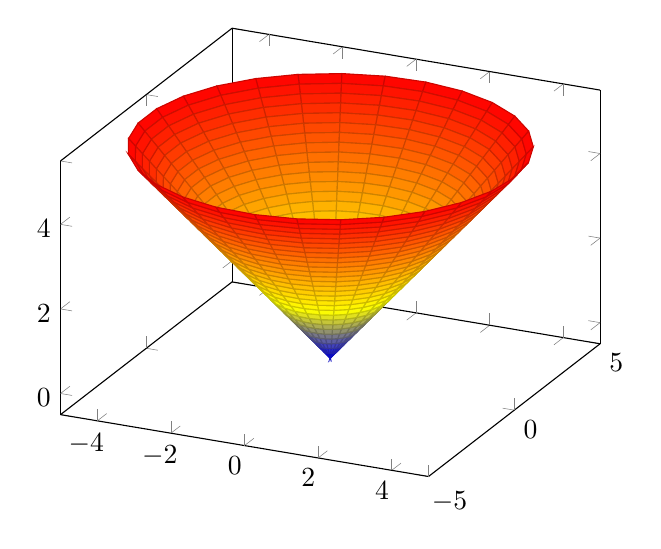
\begin{tikzpicture}
\begin{axis}[
    domain=0:5,
    y domain=0:2*pi,
    xmin=-5,
    xmax=5,
    ymin=-5,
    ymax=5,
    samples=30]
\addplot3 [surf,z buffer=sort] 
    ({x*cos(deg(y))},
     {x*sin(deg(y))},
     {x});
\end{axis}
\end{tikzpicture}
\end{center}
\item Let $S_1=\{x^2+y^2\leq 2h^2\}$. This describes a circular region at height $z=h$. The closed surface is $S=A\cup S_1$. Then $\mathbf{G}$ satisfy the divergence theorem,
$$\int_V\boldsymbol{\nabla}\cdot\mathbf{G}dV=\int_{\partial V=S}\mathbf{G}\cdot\mathbf{n}dS=\int_A\mathbf{G}\cdot\mathbf{n}dS+\int_{S_1}\mathbf{G}\cdot\mathbf{n}dS$$
We have $\boldsymbol{\nabla}\cdot\mathbf{G}=3x^2+3y^2=1$ and $\mathbf{n}$ for $S_1$ to be $\mathbf{\hat{z}}$, so
$$\int_{S_1}\mathbf{G}\cdot\mathbf{n}dS=\int_0^{2\pi}\int_0^{\sqrt{2}h}hrdrd\theta=2\pi h^3$$
We thus have
$$\int_A\mathbf{G}\cdot\mathbf{n}dS=\int_V\boldsymbol{\nabla}\cdot\mathbf{G}dV-\int_{S_1}\mathbf{G}\cdot\mathbf{n}dS=\int_0^h\int_0^{\sqrt{2}z}r(3r^2+1)drdz2\pi-2\pi h^3=\pi h^2$$
\end{enumerate}

%\begin{figure}[H]
%    \centering
%    \includegraphics[scale=0.5]{2017P1Q1.png}
%    \caption{A cone, with a circular top at $z=h$ (arbitrarily set to 1 in the plot) and vertex at the origin, where $A$ is the curved surface.}
%\end{figure}

\end{ans}
\newpage
\begin{qns}[Partial Differential Equation]
Consider the equation
$$\frac{\partial v}{\partial t}=\frac{\partial^2v}{\partial x^2}+\frac{2v}{t+1}$$
where $v(x, t)$ is defined on $0\leq x\leq \pi$ and is subject to the initial and boundary conditions
$$v(0,t)=0,\quad v(\pi,t)=f(t),\quad v(x,0)=h(x)$$
for some functions $f(t)$ and $h(x)$.
\begin{enumerate}[label=(\alph*)]
\item Using the substitution $v=(t+1)^2u$, show that $u$ satisfies the diffusion equation
$$\frac{\partial u}{\partial t}=\frac{\partial^2u}{\partial x^2}$$
and state the boundary and initial conditions satisfied by $u$.\hfill\textbf{[5]}
\item Now consider the specific case when the functions $f$ and $h$ are given by
$$f(t)=3(t+1)^2,\quad h(x)=\frac{\sin(2x)+3x}{\pi}$$
Using the method of separation of variables, construct the solution $v(x, t)$.\hfill\textbf{[13]}\\[5pt]
[Hint: You may find it helpful to use the substitution $u(x, t) = w(x, t) + \gamma x$, for a suitably chosen constant $\gamma$.]
\item For $t>>1$, show that \hfill\textbf{[2]}
$$v\sim\frac{3xt^2}{\pi}$$
\end{enumerate}
\end{qns}
\begin{ans}\leavevmode
\begin{enumerate}[label=(\alph*)]
    \item With $v=(t+1)^2u$, then $\frac{\partial v}{\partial t}=2(t+1)u+(t+1)^2\frac{\partial u}{\partial t}$, $\frac{\partial^2v}{\partial x^2}=(t+1)^2\frac{\partial^2u}{\partial x^2}$ and so $u$ satisfy the diffusion equation. The boundary and initial conditions become $$0=v(0,t)=(t+1)^2u(0,t)\implies u(0,t)=0$$ $$f(t)=v(\pi,t)=(t+1)^2u(\pi,t)\implies u(\pi,t)=\frac{f(t)}{(t+1)^2}$$
$$h(x)=v(x,0)=u(x,0)$$
\item We first substitute $u(x,t)=w(x,t)+\gamma (x)$. Then, $$\frac{\sin 2x+3x}{\pi}=h(x)=w(x,0)+\gamma x\implies w(x,0)=\frac{1}{\pi}\sin 2x$$ and $\gamma=\frac{3}{\pi}$. $u(0,t)=w(0,t)=0$ and $3=w(\pi,t)+3\implies w(\pi,t)=0$. We now have homogeneous boundary conditions and may use separation of variables, i.e. $w(x,t)=X(x)T(t)$. Note, $w(x,t)$ satisfies the same diffusion equation as $u(x,t)$.
$$\frac{T'(t)}{T(t)}=\frac{X''(x)}{X(x)}=-\lambda^2$$
The boundary condition for $w$ suggests $X(x)\sim\sin\lambda x$ and so $T(t)\sim e^{-\lambda^2t}$ with $\lambda\in\mathbb{N}$. Imposing the initial condition $\frac{1}{\pi}\sin 2x=w(x,0)=\sum_{\lambda=1}^\infty A_\lambda\sin\lambda x$ would give $A_2=\frac{1}{\pi}$ and $A_\lambda=0$ $\forall\lambda\neq 2$. We thus have
$$v(x,t)=(t+1)^2u(x,t)=\frac{(t+1)^2}{\pi}(3x+\sin 2x e^{-4t})$$
\item For $t>>1$, $e^{-4t}\approx 0$, so $v(x,t)\approx\frac{3xt^2}{\pi^2}$, as desired.
\end{enumerate}
\end{ans}
\newpage
\begin{qns}[Green's Function]
An amplifier outputs a signal $x(t)$ given by the initial-value problem
\begin{equation}
    \frac{d^2x}{dt^2}+2q\frac{dx}{dt}+(q^2+4)x=f(t),\quad x(0)=\frac{dx}{dt}(0)=0\tag{*}
\end{equation}
for some constant $q>0$ and input function $f(t)$.
\begin{enumerate}[label=(\alph*)]
\item Show that the Green’s function $G(t,\tau)$ for this problem is \hfill\textbf{[7]}
$$G(t,\tau)=
\left\{
        \begin{array}{ll}
      0 & 0\leq t<\tau \\
      \frac{1}{2}e^{-q(t-\tau)}\sin[2(t-\tau)] & \tau\leq t
        \end{array}
    \right.$$
Write down the general solution $x(t)$ of equation (*) in terms of an integral.\hfill\textbf{[2]}
\item Now consider the specific case $q = 0$ and
$$f(t)=
\left\{
        \begin{array}{ll}
      t_0 & 0\leq t<t_0 \\
      0 & t_0\leq t
        \end{array}
    \right.$$
    where $t_0>0$ is a constant. Calculate the solution of equation (*) in this case.\hfill\textbf{[8]}\\[5pt]
    Find all values of $t_0$ for which $x(t)=0$ $\forall t\geq t_0$.\hfill\textbf{[3]}
    \end{enumerate}
\end{qns}
\begin{ans}\leavevmode
\begin{enumerate}[label=(\alph*)]
\item The homogeneous solution to (*) is $x(t)=e^{-qt}(c_1\cos(2t)+c_2\sin(2t))$. The corresponding Green's function $G(t,\tau)$ satisfies
$$\frac{\partial^2G(t,\tau)}{\partial t^2}+2q\frac{\partial G(t,\tau)}{\partial t}+(q^2+4)G(t,\tau)=\delta(t-\tau),\quad G(0,\tau)=G'(0,\tau)=0$$
Integrate this around an infinitesimal region about $t=\tau$, we obtain the jump condition at $t=\tau$, i.e. $[G']_{\tau^-}^{\tau^+}=1$. $G$ is continuous everywhere, including $t=\tau$ (otherwise, $G''\propto\delta'(t-\tau)$ which is a contradiction).
Using the two linearly independent homogeneous solutions, we construct the Green's function 
$$G(t,\tau)=
\left\{
        \begin{array}{ll}
      A(\tau)e^{-qt}\sin(2t)+B(\tau)e^{-qt}\cos(2t) & 0\leq t<\tau<\infty \\
      C(\tau)e^{-q(t-\tau)}\sin2(t-\tau)+D(\tau)e^{-q(t-\tau)}\cos2(t-\tau) & 0\leq\tau<t<\infty
        \end{array}
    \right.$$
The initial conditions for $G(t,\tau)$ are $G(0,\tau)=0\implies B(\tau)=0$ and $\frac{dG}{dt}|_{t=0}=0\implies 2A(\tau)-qB(\tau)e^{-qt}=0$. Hence, $A(\tau)=B(\tau)=0$. The continuity and jump conditions at $t=\tau$ are respectively $$A(\tau)e^{-q\tau}\sin2\tau+B(\tau)e^{-q\tau}\cos 2\tau=D(\tau)\implies D(\tau)=0$$ $$2C(\tau)-qD(\tau)-2A(\tau)+qB(\tau)=1\implies C(\tau)=0.5$$ Hence, we have our desired $G(t,\tau)$. The general solution would be
$$x(t)=\int_0^\infty f(\tau)G(t,\tau)d\tau=\int_0^t\frac{1}{2}e^{-q(t-\tau)}\sin[2(t-\tau)]f(\tau)d\tau$$
\item  Consider $q=0$. For $t\leq t_0$, 
$$x(t)=\int_0^tt_0\frac{1}{2}\sin[2(t-\tau)]d\tau=\frac{t_0}{4}(1-\cos 2t)$$
For $t>t_0$,
$$x(t)=\int_0^{t_0}t_0\frac{1}{2}\sin[2(t-\tau)]dt=\frac{t_0}{4}[\cos[2(t_0-t)]-\cos(2t)]=\frac{t_0}{4}[\cos(2t)(\cos(2t_0)-1)-\sin2t_0\sin 2t]$$
For $x(t)=0$ $\forall t>t_0$, $\sin 2t_0=0$ and $\cos 2t_0=1$, and so $t_0=n\pi$ for $n\in\mathbb{Z}$.
\end{enumerate}
\end{ans}
\newpage
\begin{qns}[Fourier Transform]\leavevmode
\begin{enumerate}[label=(\alph*)]
\item The Fourier transform of a function $f(t)$ is given by
$$\tilde{f}(\omega)=\int_{-\infty}^\infty f(t)e^{-i\omega t}dt$$
Write down the corresponding expression for the inverse Fourier transform.\hfill\textbf{[2]}
\item Consider the convolution of the functions $f$ and $g$
$$h(z)=\int_{-\infty}^\infty f(t)g(z-t)dt$$
Prove that the Fourier transform of $h$ is given by the product of the Fourier
transforms of $f$ and $g$.\hfill\textbf{[5]}
\item Find the Fourier transform of
$$f(\gamma,p,t)=
\left\{
        \begin{array}{ll}
      e^{-\gamma t}\sin(pt) & t>0 \\
      0 & t\leq 0
        \end{array}
    \right.$$
    where $\gamma>0$ and $p$ are fixed parameters.\hfill\textbf{[6]}\\[5pt]
    [Hint: Write $\sin(pt)$ in terms of exponential functions.]
\item  The current $I(t)$ flowing through a system is related to the applied voltage $V (t)$ by the equation  
$$I(t)=\int_{-\infty}^\infty K(t-u)V(u)du$$
where
$$K(\tau)=a_1f(\gamma_1,p_1,\tau)+a_2f(\gamma_2,p_2,\tau)$$
Here the function $f(\gamma,p,t)$ is as given in part (c), and all the $a_i$, $\gamma_i>0$ and $p_i$ are fixed parameters. By considering the Fourier transform of $I(t)$, find the relationship that must hold between $a_1$ and $a_2$ if the net charge $Q$, defined by
$$Q=\int_{-\infty}^\infty I(t')dt'$$
is to be zero for an arbitrary applied voltage.\hfill\textbf{[7]}
\end{enumerate}
[Hint: $\int_{-\infty}^\infty e^{i\omega t'}dt'=2\pi\delta(\omega)$.]
\end{qns}
\begin{ans}\leavevmode
\begin{enumerate}[label=(\alph*)]
\item The inverse Fourier transform will be $f(t)=\frac{1}{2\pi}\int_{-\infty}^\infty\tilde{f}(\omega)e^{+i\omega t}d\omega$.
\item Evaluate the Fourier transform of $h(z)$, $\tilde{h}(\omega)$:
$$\int_{-\infty}^\infty\int_{-\infty}^\infty f(t)g(z-t)~dt~e^{-i\omega z}dz=\int_{-\infty}^\infty\int_{-\infty}^\infty f(t)g(u)e^{-i\omega(u+t)}dudt=\int_{-\infty}^\infty f(t)e^{-i\omega t}dt\int_{-\infty}^\infty g(u)e^{-i\omega u}du$$
which is $\tilde{f}(\omega)\tilde{g}(\omega)$, where we swap integration order, substitute $u=z-t$ and finally separate the integral.
\item Write $f(\gamma,p,t>0)=e^{-\gamma t}\frac{1}{2i}(e^{ipt}-e^{-ipt})$, so the Fourier transform is
$$\tilde{f}(\gamma,p,\omega)=\frac{1}{2i}\int_0^\infty e^{(-\gamma+i(p-\omega))t}+e^{(-\gamma-i(p+\omega))t}dt=\frac{1}{2i}\bigg[\frac{1}{\gamma+i(\omega-p)}-\frac{1}{\gamma+i(\omega+p)}\bigg]$$
\item By the convolution theorem, the Fourier transform is $\tilde{I}(\omega)=\tilde{K}(\omega)\tilde{V}(\omega)=\tilde{V}(\omega)[a_1\tilde{f}(\gamma_1,p_1,\omega)+a_2\tilde{f}(\gamma_2,p_2,\omega)]$. Given $Q=\int_{-\infty}^\infty I(t')dt'=0$ for any arbitrary $V(u)$. We thus have $\frac{dQ}{dt}=I(t)=0\implies i\omega Q=\tilde{I}(\omega)=0\implies\tilde{K}(\omega)=0$ $\forall\omega$. For convenience, let $\omega=0$, then $\tilde{K}(0)=0$.
$$0=a_1\bigg(\frac{p_1}{-p_1^2-\gamma_1^2}\bigg)+a_2\bigg(\frac{p_2}{-p_2-\gamma_2^2}\bigg)\implies\frac{a_1}{a_2}=-\frac{p_2}{p_1}\frac{p_1^2+\gamma_1^2}{p_2^2+\gamma_2^2}$$
\end{enumerate}
\end{ans}
\begin{qns}[Linear Algebra]\leavevmode
\begin{enumerate}[label=(\alph*)]
\item When is an $n\times n$ matrix $A$ diagonalisable? Give an example of a non-diagonalizable $n\times n$ matrix (for some $n$). What is a Hermitian matrix? Show that the eigenvalues of a Hermitian matrix are real, and that the corresponding eigenvectors are orthogonal.\hfill\textbf{[5]}
\item Diagonalize the matrix
$$A=\begin{pmatrix}2&-a&0\\-a&2&0\\0&0&c\\\end{pmatrix}$$
where $a>0$ and $c>0$ are real numbers and finds its eigenvectors.\hfill\textbf{[6]}
\item Sketch the surface
$$\mathbf{x}^TA\mathbf{x}=1$$
where $\mathbf{x}=(x,y,z)$, specifying the principal axes and, where appropriate, the semi-axis lengths. Note that different values of a may correspond to different surfaces.\hfill\textbf{[9]}
\end{enumerate}
\end{qns}
\begin{ans}\leavevmode
\begin{enumerate}[label=(\alph*)]
\item An $n\times n$ matrix $A$ is diagonalizable if it has $n$ linearly independent eigenvectors. We can then place the $n$ linearly independent eigenvectors into the columns of $n\times n$ matrix $P$ such that $P^TAP$ is a diagonal matrix.\\[5pt]
An example is $M=\begin{pmatrix}1&1\\0&1\\\end{pmatrix}$. Since $M$ is block diagonal, then the eigenvalues are easily determined to be $1$ and 1. If $M$ were diagonalizable, there exists a transformation such that $RMR^{-1}=I$, which imply $M=R^{-1}IR=I$. A contradiction, so $M$ is not diagonalizable.\\[5pt]
A Hermitian matrix $H$ has the property that for all the vectors $\mathbf{a}$, $\mathbf{b}$, we have $\langle \mathbf{a}|H\mathbf{b}\rangle=\langle H\mathbf{a}|\mathbf{b}\rangle$. This is equivalent to stating $H=H^\dag=(H^T)^*$.\\[5pt]
Let the eigenvectors $\mathbf{e_n}$ and eigenvalues $\lambda_n$ of $H$ satisfy $H\mathbf{e_n}=\lambda_n\mathbf{e_n}$. Then,
$$0=\langle e_p|He_n\rangle-\langle He_p|e_n\rangle=(\lambda_n-\lambda_p^*)\langle e_p|e_n\rangle$$
If we choose $n=p$, then since $\langle e_n|e_n\rangle>0$, we have $\lambda_n=\lambda_p^*=\lambda_n^*\in\mathbb{R}$. If the eigenvalues are distinct, $n\neq p$ and $\lambda_n\neq\lambda_p^*=\lambda_p$, and so $\langle e_n|e_p\rangle=0$, i.e. the eigenvectors corresponding to distinct eigenvalues are orthogonal.\\[5pt]
Suppose there are $n$ distinct eigenvalues for the $n\times n$ Hermitian matrix, then we can automatically find $n$ linearly independent orthogonal eigenvectors.\\[5pt]
But suppose there are only $r<n$ distince eigenvalues, i.e. the eigenvalues are degenerate, then there must exist at least one direction which possesses one of the degenerate eigenvalues, say $\lambda$, and is the corresponding eigenvector. Construct an orthonormal basis for the $n$-dimensional space consisting of that direction and any orthonormal basis in the orthogonal complement. In this basis $\{\mathbf{e_n}\}$ (where $\mathbf{e_1}$ is the known direction with eigenvalue $\lambda$), then in this basis, $H$ has the form
$$H=\begin{pmatrix}\langle e_1|He_1\rangle&\langle e_1|He_2\rangle&\dots\\\langle e_2|He_1\rangle&\langle e_2|He_2\rangle&\dots\\\vdots&\vdots&\ddots\\\end{pmatrix}=\begin{pmatrix}\lambda_1&0&\dots\\0&\langle e_2|He_2\rangle&\dots\\\vdots&\vdots&\ddots\\\end{pmatrix}$$
where $\langle e_1|e_2\rangle=0$. $e_2$ is not assumed to be an eigenvector. Having to decompose the space into the direct sum of $\mathbf{e_1}$ and its orthogonal complement, we restrict ourselves to the $(n-1)\times(n-1)$ subspace where a copy of the degenerate eigenvalue $\lambda$ has been removed from the characteristic equation. We repeat the above process until each copy of the degenerate eigenvalue has been given an orthogonal eigenvector. This set of orthogonal eigenvectors is not unique. With this orthogonal basis, we can construct a matrix $P$ to diagonalize $H$.
\item The determinant is
$$0=\det(A-\lambda I)=\det\begin{pmatrix}2-\lambda&-9&0\\-9&2-\lambda&0\\0&0&c-\lambda\\\end{pmatrix}=(c-\lambda)\begin{vmatrix}2-\lambda&-a\\-a&2-\lambda\\\end{vmatrix}=(c-\lambda)[(2-\lambda)^2-a^2]$$
$\lambda=c,2\pm a$. By inspection, the eigenvector is found to be $\mathbf{e}_{\lambda=c}=(0,0,1)^T$. For $\lambda=2+a$, we evaluate $(A-(2+a)I)x=0$ and show that $\mathbf{e}_{\lambda=2+a}=\frac{1}{\sqrt{2}}(1,-1,0)^T$. Since $A$ is Hermitian, the set of eigenvectors must be mutually orthogonal. So the last eigenvector is $\mathbf{e}_{\lambda=2-a}=\frac{1}{\sqrt{2}}(1,1,0)^T$. Hence, $A=R\Lambda R^T$:
$$A=\begin{pmatrix}1/\sqrt{2}&1/\sqrt{2}&0\\-1/\sqrt{2}&1/\sqrt{2}&0\\0&0&1\\\end{pmatrix}\begin{pmatrix}2+a&0&0\\0&2-a&0\\0&0&c\\\end{pmatrix}\begin{pmatrix}1/\sqrt{2}&-1/\sqrt{2}&0\\1/\sqrt{2}&1/\sqrt{2}&0\\0&0&1\\\end{pmatrix}$$
\item The quadratic surface is 
$$1=x^TAx=x^TR\Lambda R^Tx=U^T\Lambda U,\quad U=R^Tx=\begin{pmatrix}\frac{1}{\sqrt{2}}(x-y)\\\frac{1}{\sqrt{2}}(x+y)\\z\\\end{pmatrix}$$
In $u$ coordinates, $$1=u_1^2(2+a)+u_2^2(2-a)+u_3^2c$$
where the $u_3$-axis coincide with the $z$-axis.
\begin{itemize}
    \item $a=0,c=2$: $1=2(u_1^2+u_2^2+u_3^2)$ is a sphere of radius $\frac{1}{\sqrt{2}}$;
    \item $a=0,c<2$: $1=2u_1^2+2u_2^2+u_3^2c$ is a prolate ellipsoid of revolution about the $z$-axis with major axis length $\frac{1}{\sqrt{c}}$ and minor axis length $\frac{1}{\sqrt{2}}$;
    \item $a=0,c>2$: $1=2u_1^2+2u_2^2+u_3^2c$ is an oblate ellipsoid of revolution about the $z$-axis with major axis length $\frac{1}{\sqrt{2}}$ and minor axis length $\frac{1}{\sqrt{c}}$;
    \item $a<2$: triaxial ellipsoid with principal axes being eigenvectors and semi-axes lengths being $\frac{1}{\sqrt{2+a}}$, $\frac{1}{\sqrt{2-a}}$ and $\frac{1}{\sqrt{c}}$;
    \item $a=2$: $1=4u_1^2+cu_3^2$ is an ellipsoidal cylinder with cylindrical axis in $\mathbf{e_2}$ and elliptical cross-section in $e_1$-$e_3$ plane with semi-axes of lengths $\frac{1}{\sqrt{2+a}}$ and $\frac{1}{\sqrt{c}}$;
    \item $a>2$: hyperboloid of one sheet, with elliptical cross-section in $e_1$-$e_3$ plane and $e_2$ being the symmetry axis.
\end{itemize}
\end{enumerate}
\end{ans}
\newpage
\begin{qns}[Linear Algebra]\leavevmode
\begin{enumerate}[label=(\alph*)]
\item Let $A$ and $B$ be $n\times n$ Hermitian matrices, each with n distinct eigenvalues. Show that:
\begin{enumerate}[label=(\roman*)]
\item the matrix $H = i(AB − BA)$ is Hermitian;\hfill\textbf{[4]}
\item the eigenvectors of $A$ and $B$ are identical if and only if $AB = BA$;\hfill\textbf{[6]}
\item the matrix $N = A + iB$ is diagonalisable.\hfill\textbf{[5]}
\end{enumerate}
\item Suppose $C$ is a unitary matrix, $A$ is a Hermitian matrix, and $p$ is a positive integer. Show that $(C^{−1}AC)^p$ has real eigenvalues.\hfill\textbf{[5]}
\end{enumerate}
\end{qns}
\begin{ans}\leavevmode
\begin{enumerate}[label=(\alph*)]
\item 
\begin{enumerate}[label=(\roman*)]
\item This is true. Since $A$ and $B$ are Hermitian, i.e. $A^\dag=A$ and $B^\dag=B$, 
$$H^\dag=-i(AB-BA)^\dag=-i(B^\dag A^\dag-A^\dag B^\dag)=-i(BA-AB)=i(AB-BA)=H$$
\item Assume the eigenbasis of $A$ is also the eigenbasis of $B$. Let this be $\{\mathbf{e_n}\}$ such that $A\mathbf{e_n}=a_n\mathbf{e_n}$ and $B\mathbf{e_n}=b_n\mathbf{e_n}$. Since each eigenvalue is distinct, the eigenvectors are linearly independent, i.e. the only solution to $\mathbf{q}=\sum_{p=1}^n\alpha_p\mathbf{e_p}=\boldsymbol{0}$ is $\alpha_p=0$ $\forall p$. Consider
$$\boldsymbol{0}=\prod_{p=1,p\neq s}^n(A-a_pI)\mathbf{q}=\prod_{p=1,p\neq s}^n(a_s-a_p)\alpha_s\mathbf{e_s}$$
which implies $\alpha_s=0$ $\forall\mathbf{e_s}$, so the eigenvectors form a basis. Apply $AB-BA$ to an arbitrary vector $\mathbf{v}=\sum_{p=1}^n\beta_p\mathbf{e_p}$ written as a linear combination of the basis vectors:
$$(AB-BA)\mathbf{v}=\sum_{p=1}^n(a_pb_p-b_pa_p)\beta_p\mathbf{e_p}=\boldsymbol{0}\implies AB=BA$$
Conversely, if $AB=BA$, then $a_nB\mathbf{e_n}=AB\mathbf{e_n}=BA\mathbf{e_n}$, and so $B\mathbf{e_n}$ is an eigenvector of $A$ with eigenvalue $a_n$. But all the eigenvalues of $A$ are given to be distinct, so $B\mathbf{e_n}$ is parallel to $\mathbf{e_n}$, $\exists b_n$ such that $Be_n=b_ne_n$. Hence, the eigenvectors of $A$ are also the eigenvectors of $B$.
\item This is not true! We can rewrite $N$ as
$$N=\frac{1}{2}(N+N)+\frac{1}{2}(N^\dag-N^\dag)=\frac{1}{2}(N+N^\dag)+i\frac{1}{2i}(N-N^\dag)$$
We label $A=\frac{1}{2}(N+N^\dag)$ and $B=\frac{1}{2i}(N-N^\dag)$. We give a quick example of a non-diagonalizable matrix. Let $N=\begin{pmatrix}1&2\\0&1\\\end{pmatrix}$. The eigenvalues are 1 and 1. If the matrix were diagonalizable, $\exists U$ such that $U^\dag NU=I$. But, $N=UIU^\dag=I$, which is a contradiction. For this choice of $N$, we choose $A=\begin{pmatrix}1&1\\1&1\\\end{pmatrix}$ and $B=\begin{pmatrix}0&-i\\i&0\\\end{pmatrix}$. Indeed, both are Hermitian matrices and have 2 distinct eigenvalues, namely $\{2,0\}$ and $\{+1,-1\}$ respectively. But yet, $N$ is not diagonalizable.
\end{enumerate}
\item $A$ is Hermitian and must have real eigenvalues. Take $Ae_n=a_ne_n$. 
$$0=\langle e_n|Ae_n\rangle-\langle Ae_n|e_n\rangle=(a_n-a_n^*)\langle e_n|e_n\rangle$$
Since $\langle e_n|e_n\rangle\neq 0$, $a_n=a_n^*\in\mathbb{R}$. So consider $v_n=C^\dag e_n$, then
$$(C^{-1}AC)^pC^\dag e_n=C^{-1}ACC^\dag e_n=C^{-1}A^pe_n=a_n^pC^{-1}e_n=a_n^pC^\dag e_n$$
where $C$ is unitary. So, $C^\dag e_n$ is an eigenvector of $(C^{-1}AC)^p$. Since $a_n\in\mathbb{R}\implies a_n^p\in\mathbb{R}$, then $(C^{-1}AC)^p$ have real eigenvalues.
\end{enumerate}
\end{ans}
\newpage
\begin{qns}[Cauchy-Riemann]\leavevmode
\begin{enumerate}[label=(\alph*)]
\item Use the Cauchy-Riemann relations to show that, for any analytic function $f(x,y)=u(x,y)+iv(x,y)$, the relation $|\nabla u| = |\nabla v|$ must hold.\hfill\textbf{[2]}
\item Find the most general analytic function $f(z)$ of the variable $z = x + i y$ whose imaginary part is
$$(y\cos y + x\sin y)e^x$$
(Your final expression for $f(z)$ should be in terms of $z$, not $x$ and $y$.)\hfill\textbf{[10]}
\item Find the radii of convergence of the following Taylor series:
\begin{enumerate}[label=(\roman*)]
\item \hfill\textbf{[3]}$$\sum_{n=2}^\infty\frac{z^n}{\ln n}$$
\item  \hfill\textbf{[5]}
$$\sum_{n=1}^\infty\bigg(\frac{n+p}{n}\bigg)^{n^2}z^n,\text{ with  }p\in\mathbb{R}$$
\end{enumerate}
\end{enumerate}
\begin{mdframed}
\textcolor{darkblue}{Hint: You may want to use the following result:
$$a^n=e^{n\ln a}$$
for some real $a$.}
\end{mdframed}
\end{qns}
\begin{ans}\leavevmode
\begin{enumerate}[label=(\alph*)]
\item The Cauchy-Riemann relations are $\frac{\partial u}{\partial x}=\frac{\partial v}{\partial y}$ and $\frac{\partial u}{\partial y}=-\frac{\partial v}{\partial x}$. If $f$ is analytic, then
$$|\boldsymbol{\nabla}u|=\sqrt{\bigg(\frac{\partial u}{\partial x}\bigg)^2+\bigg(\frac{\partial u}{\partial y}\bigg)^2}=\sqrt{\bigg(\frac{\partial v}{\partial y}\bigg)^2+\bigg(-\frac{\partial v}{\partial x}\bigg)^2}=|\boldsymbol{\nabla}v|$$
\item  $\text{Im}[f]=(y\cos y+x\sin y)e^x$. For $f=u+iv$ to be analytic, it must be complex differentiable and obeys the Cauchy-Riemann relations. So
$$-\frac{\partial u}{\partial y}=\frac{\partial v}{\partial x}=e^x\sin y+e^x(y\cos y+x\sin y)\implies u(x,y)=\cos ye^x-\int y\cos ydy e^x+e^x x\cos y+g(x)$$
$$\frac{\partial u}{\partial x}=\frac{\partial v}{\partial y}=\cos y e^x-y\sin y e^x+x\cos ye^x\implies u(x,y)=e^x(\cos y-y\sin y)+\cos y\int xe^xdx+h(y)$$
But $\int y\cos ydy=y\sin y+\cos y$ and $\int xe^xdx=e^x(x-1)$ and so comparing both expressions, $u(x,y)=(x\cos y-y\sin y)e^x+C$ where $C$ is some constant. Thus,
$$f(x,y)=u(x,y)+iv(x,y)=(x\cos y-y\sin y)e^x+i(y\cos y+x\sin y)e^x+C=ze^xe^{iy}+C=ze^z+C$$
\item 
\begin{enumerate}[label=(\roman*)]
\item Try ratio test with $u_n(z)=\frac{z^n}{\ln n}$ for $n\geq 2$:
$$1=\lim_{n\rightarrow\infty}\bigg|\frac{u_{n+1}(R)}{u_n(R)}\bigg|=\lim_{n\rightarrow\infty}\frac{R^{n+1}}{R^n}\frac{\ln n}{\ln n+1}=R\lim_{n\rightarrow\infty}\frac{1/n}{1/(n+1)}=R$$
where we used L'Hopital Rule.
\item Try ratio test with $u_n(z)=(\frac{n+p}{n})^{n^2}z^n$ for $n\geq 1$:
$$1=\lim_{n\rightarrow\infty}\bigg|\frac{u_{n+1}(R)}{u_n(R)}\bigg|=\lim_{n\rightarrow\infty}\bigg|\frac{R^{n+1}}{R^n}\bigg(\frac{n+1+p}{n+1}\bigg)^{(n+1)^2}\bigg(\frac{n}{n+p}\bigg)^{n^2}\bigg|=R\lim_{n\rightarrow\infty}e^{(n+1)p-np}=Re^p$$
where we used the given hint, as well as, the approximation $\ln(1+\frac{p}{n+1})\approx\frac{p}{n+1}$ for large $n$. Hence, $R=e^{-p}$.
\end{enumerate}
\end{enumerate}
\end{ans}
\newpage
\begin{qns}[Series Solution to ODE]\leavevmode
\begin{enumerate}[label=(\alph*)]
\item Find the power series solution of the equation
\begin{equation}
\frac{d^2y}{dx^2}-2x\frac{dy}{dx}+\lambda y=0\tag{*}
\end{equation}
where $\lambda$ is a real parameter, about the point $x = 0$, and find suitable recurrence relations for the coefficients. For what values of $\lambda$ does (*) have a polynomial solution? Find the solutions corresponding to two eigenvalues $\lambda$ of your choice.\hfill\textbf{[10]}
\item Consider the hypergeometric equation
$$x(1-x)\frac{d^2y}{dx^2}+[\gamma-(1+\alpha+\beta)x]\frac{dy}{dx}-\alpha\beta y=0$$
where $\alpha$, $\beta$ and $\gamma$ are real constants. Assuming a solution of the form
$$y(x)=\sum_{n=0}^\infty a_nx^{n+\sigma}\text{ with }a_0\neq 0$$
show that
$$\sigma=0\text{ or   }\sigma=1-\gamma$$
and that
$$a_n=\frac{(n+\sigma+\alpha-1)(n+\sigma+\beta-1)}{(n+\sigma)(n+\sigma+\gamma-1)}a_{n-1}$$
for all $n\geq1$.\hfill\textbf{[10]}
\end{enumerate}
\end{qns}
\begin{ans}\leavevmode
\begin{enumerate}[label=(\alph*)]
\item $-2x$ and $\lambda$ are analytic at $x=0$, so $x=0$ is an ordinary point. We can try a series solution of the form $y=\sum_{n=1}^\infty a_nx^n$. The recurrence relation will be
$$\sum_{n=1}^\infty a_nn(n-1)x^{n-2}-2\sum_{n=1}^\infty a_nnx^n+\lambda\sum_{n=1}^\infty a_nx^n=0\implies a_{n+2}=\frac{2n-\lambda}{(n+2)(n+1)}a_n$$
To have a polynomial solution, the series must terminate. This means $\lambda=2n$, i.e. $\lambda$ is even. We have $a_2=-\frac{\lambda}{2}a_0$ and $a_3=\frac{2-\lambda}{3\times 2}a_1$. We choose $\lambda=0\implies y=a_0$ and $\lambda=2\implies y=a_1x$.
\item With the suggested series solution and comparing the $x^{n+\sigma}$ terms with $n\geq 1$ will give the recurrence relation
\begin{eqnarray}
0&=&\sum_{n=0}^\infty a_n(n+\sigma)(n+\sigma-1)x^{n+\sigma-1}-\sum_{n=0}^\infty a_n(n+\sigma)(n+\sigma-1)x^{n+\sigma}\nonumber\\&&+\gamma\sum_{n=0}^\infty a_n(n+\sigma)x^{n+\sigma-1}-\sum_{n=0}^\infty[(1+\alpha+\beta)(n+\sigma)-\alpha\beta] a_n x^{n+\sigma}\nonumber\\\implies a_{n+1}&=&\frac{(n+\sigma+\alpha)(n+\sigma+\beta)}{(n+1+\sigma)(n+\sigma+\gamma)}a_n\nonumber
\end{eqnarray}
Reindexing give the desired relation. Comparing the $x^{\sigma-1}$ terms give $a_0\sigma(\gamma+\sigma-1)=0$. Since $a_0\neq 0$, $\sigma=0$ or $\sigma=1-\gamma$.
\end{enumerate}
\end{ans}
\newpage
\begin{qns}[Variational Principle]\leavevmode
\begin{enumerate}[label=(\alph*)]
\item The Euler–Lagrange equation for extrema of the functional
$$D[y]=\int_a^bf(x,y,y')dx$$
where $y'=\frac{dy}{dx}$ is
\begin{equation}
\frac{\partial f}{\partial y}-\frac{d}{dx}\bigg(\frac{\partial f}{\partial y'}\bigg)=0\tag{*}
\end{equation}
If $f = f(y, y')$ does not depend explicitly on $x$ show that (*) can be written as
$$\frac{dh}{dx}=0$$
for some $h$, which you should determine.\hfill\textbf{[3]}
\item A forest lies in the $(x, y)$ plane. A new path through the forest is proposed, starting at $(x, y) = (−1, 1)$ and ending at $(x, y) = (1, 1)$. The density of undergrowth in the forest is given by $g(y)$, such that the total undergrowth $D$ to be destroyed by the new path is
$$D=\int_{\mathcal{P}}g(y)ds$$
where $ds$ is the arc-length element along the path $\mathcal{P}$.
\begin{enumerate}[label=(\roman*)]
\item Given that the path always travels in the positive $x$ direction, show that the path $y(x)$ that minimises the destruction of undergrowth satisfies\hfill\textbf{[4]}
$$\frac{d}{dx}\bigg(\frac{g}{\sqrt{1+y'^2}}\bigg)=0$$
\item In the specific case when $g=y^{-1}$, calculate the path $y(x)$. \hfill\textbf{[9]}
\item Sketch the path, and determine its length.\hfill\textbf{[4]}
\end{enumerate}
\end{enumerate}
\end{qns}
\begin{ans}\leavevmode
\begin{enumerate}[label=(\alph*)]
\item By chain rule and invoke Euler-Lagrange equation (*):
$$\frac{df}{dx}=\frac{\partial f}{\partial x}+\frac{\partial f}{\partial y}\frac{\partial y}{\partial x}+\frac{\partial f}{\partial y'}\frac{\partial y'}{\partial x}=\frac{\partial f}{\partial x}+y'\frac{d}{dx}\frac{\partial f}{\partial y'}+y''\frac{\partial f}{\partial y'}=\frac{\partial f}{\partial x}+\frac{d}{dx}y'\frac{\partial f}{\partial y'}$$
Since $f=f(y,y')$ does not explicitly depend on $x$, then $h:=y'\frac{\partial f}{\partial y'}-f$ is a constant.
\item
\begin{enumerate}[label=(\roman*)]
\item
$D=\int_{\mathcal{P}}g(y)\sqrt{dx^2+dy^2}=\int_{x>0}g(y)\sqrt{1+y'^2}dx$. The integrand is independent of $x$ and hence by part (a),
$$0=\frac{d}{dx}\bigg(g(y)\sqrt{1+y'^2}-\frac{y'g}{\sqrt{1+y'^2}}\bigg)=\frac{d}{dx}\frac{g}{\sqrt{1+y'^2}}$$
\item With $g(y)=y^{-1}$, then $y^{-1}=k\sqrt{1+y'^2}$ for some constant $k$. This simplifies to
$$y^{-2}=k^2(1+y'^2)\implies dx=\frac{ky}{\sqrt{1-k^2y^2}}dy\implies(x-x_0)^2+y^2=\frac{1}{k^2}$$
which describes an arc of a circle. The boundary conditions $y(x=\pm 1)=1$ gives $x_0=0$ and $\frac{1}{A^2}=2$. This describes an arc of a circle of radius $\sqrt{2}$.
\item The path will be a circular arc traversed clockwise form $(-1,1)$ to $(+1,1)$. The arc length will be $\frac{\pi}{2}\sqrt{2}$ (where we notice that the line from the origin to (1,1) subtends an angle of $\pi/4$ and by symmetry, the angle subtended by the arc is $\pi/2$).
\end{enumerate}
\end{enumerate}
\end{ans}
\newpage
\begin{qns}[Rayleigh-Ritz Method]\leavevmode
\begin{enumerate}[label=(\roman*)]
\item Consider the problem
\begin{equation}
    \frac{d^2u}{dx^2}+\epsilon\bigg[x\frac{d^2u}{dx^2}+\frac{du}{dx}-u\bigg]=-\lambda u,\quad0\leq x\leq\pi,\quad u'(0)=u(\pi)=0\tag{*}
\end{equation}
where $\epsilon\geq0$ is a parameter, $\lambda$ is a real constant, and $u'=\frac{du}{dx}$. Express (*) in the form
\begin{equation}
    \mathcal{L}u=\lambda u\tag{**}
\end{equation}
where $\mathcal{L}$ is an operator in Sturm-Liouville form.\hfill\textbf{[2]}
\item Now consider the functional
$$I[v]=\int_0^\pi(pv'^2+qv^2)dx$$
where $v(x)$ satisfies $v'(0) = v(\pi) = 0$, and is subject to the constraint
$$\int_0^\pi wv^2dx=1$$
for smooth functions $p(x) > 0$, $q(x) > 0$ and $w(x) > 0$. Show that, for a particular choice of the functions $p$, $q$ and $w$, which should be specified, finding extrema of $I$ is equivalent to finding solutions of (*). Explain why the stationary values of $I$ are the eigenvalues $\lambda$ of equation (**). You may use the Euler–Lagrange equation without proof.\hfill\textbf{[8]}
\item When $\epsilon=0$, show that the smallest eigenvalue of (**) is $\lambda_0=1/4$, and the associated normalised eigenfunction is
$$U_0(x)=\sqrt{\frac{2}{\pi}}\cos\frac{x}{2}$$
Using $U_0(x)$ as a trial function, find an upper bound for the lowest eigenvalue $\lambda$ of equation (**) when $\epsilon>0$.\hfill\textbf{[10]}
\end{enumerate}
\end{qns}
\begin{ans}\leavevmode
\begin{enumerate}[label=(\roman*)]
\item Rearranging gives $\mathcal{L}=-\frac{d}{dx}[(1+\epsilon x)\frac{d}{dx}]+\epsilon$.
\item We have to extremize $\int_0^\pi pv'^2+qv^2-\mu wv^2dx$. The integrand $f(v,v';x)=pv'^2+qv^2-\mu wv^2$ must satisfy Euler-Lagrange equation whenever the functional is stationary. Hence,
$$0=\frac{d}{dx}\frac{\partial f}{\partial v'}-\frac{\partial f}{\partial v}=\frac{d}{dx}(2pv')-2qv+2\mu wv\implies\frac{1}{w}\bigg(-\frac{d}{dx}\bigg(p\frac{dv}{dx}\bigg)+qv\bigg)=\mu v$$
This is equivalent to the original SL problem, where $p(x)=1+\epsilon x$, $q=\epsilon$, $\mu=\lambda$ and $w=1$. So finding extrema of $I$ (subject to the constraint) will be equivalent to finding the solutions of (**). 
$$I[v]=\int_0^\pi pv'^2+qv^2dv=[vpv']_0^\pi+\int_0^\pi-v(pv')'+vqvdx=\int_0^\pi v\bigg(-\frac{d}{dx}\bigg(p\frac{dv}{dx}\bigg)+qv\bigg)dx=\int_0^\pi vw\mathcal{L}vdx$$
where we are given $v'(0)=v(\pi)=0$, hence the boundary terms is zero. The result is just $\int_0^\pi vw\lambda vdx=\lambda$. 
The stationary values of $I$ is indeed the corresponding eigenvalues of (**).
\item When $\epsilon=0$, $\frac{d^2u}{dx^2}=-\lambda u$. For $\lambda\neq 0$, we have $u(x)=A(\lambda)\sin\sqrt{\lambda x}+B(\lambda)\cos\sqrt{\lambda}x$. The boundary conditions give $A(\lambda)=0$ $\forall\lambda$ and $\sqrt{\lambda}\pi=\frac{\pi}{2}(2n+1)$. Hence, $\lambda_0=\frac{1}{4}$ ($n=0$). To find $B_0$, we normalize:
$$1=\int_0^\pi|B_0|^2\cos^2\frac{x}{2}dx\implies B_0=\sqrt{\frac{2}{\pi}}$$
Since $w=1$, $U_0(x)=\sqrt{\frac{2}{\pi}}\cos\frac{x}{2}$ is automatically normalized. Then
$$\Lambda[U_0]=I[U_0]=\frac{2}{\pi}\int_0^\pi(1+\epsilon x)\frac{1}{4}\sin^2\frac{x}{2}+\epsilon\cos^2\frac{x}{2}dx=\frac{1}{4}+\epsilon+0-\frac{\epsilon}{4\pi}\int_0^\pi x\cos xdx=\frac{1}{4}+\epsilon\bigg(1-\frac{1}{2\pi}\bigg)$$
which is larger than $\frac{1}{4}$ for $\epsilon>0$. Thus, an upper bound for the lowest eigenvalue $\lambda_0=\frac{1}{4}$.
\end{enumerate}
\end{ans}
\newpage
\subsection{Paper 2}
\begin{qns}[Sturm-Liouville]
Let $y_n(x)$ and $\lambda_n$, $n = 0, 1, 2...$, be the real normalised eigenfunctions and corresponding eigenvalues for the Sturm–Liouville eigenvalue problem
$$\mathcal{L}y_n(x)=-\frac{d}{dx}\bigg[p(x)\frac{dy_n(x)}{dx}\bigg]+q(x)y_n(x)=\lambda_nw(x)y_n(x),\quad  0\leq x\leq 1,~y_n(0)=y_n(1)=0$$
with $p(x)>0$ and $w(x)>0$.
\begin{enumerate}[label=(\alph*)]
\item State, without proof, the orthonormality property for two eigenfunctions $y_n(x)$ and $y_m(x)$.

\hfill\textbf{[2]}
\item Given the completeness of the eigenfunctions, any real function $f(x)$ satisfying the same boundary conditions as $y_n(x)$ can be written as
$$f(x)=\sum_{n=0}^\infty a_ny_n(x)$$
for some real constants $a_n$. Show that\hfill\textbf{[5]}
$$\int_0^1w(x)f(x)^2dx=\sum_{n=0}^\infty a_n^2$$
\item Now consider the equation $\mathcal{L}Y(x)=w(x)[\alpha Y(x)+f(x)]$, where $\alpha$ is a constant, $\alpha\neq\lambda_n$ for any $n$, and $Y (x)$ satisfies the same boundary conditions as $y_n(x)$.
\begin{enumerate}[label=(\roman*)]
\item Show that the solution of this equation can be written as\hfill\textbf{[6]}
$$Y(x)=\sum_{n=0}^\infty\frac{a_n}{\lambda_n-\alpha}y_n(x)$$
\item Suppose that $\lambda_0=1$, $\lambda_1=2$, and $f = 2 [y_0(x) + y_1(x)] −\alpha y_1(x)$. Given that
$$\int_0^1w(x)Y(x)^2dx=2$$
and that $\alpha>0$, find $\alpha$ and express $Y (x)$ in terms of the eigenfunctions $y_n(x)$.\hfill\textbf{[7]}
\end{enumerate}
\end{enumerate}
\end{qns}
\begin{ans}\leavevmode
\begin{enumerate}[label=(\alph*)]
\item $\int_0^1y_n(x)w(x)y_m(x)=\delta_{mn}$.
\item Using the result of part (a):
$$\int_0^1w(x)f(x)^2dx=\int_0^1w(x)\sum_{p=0}^\infty a_py_p(x)\sum_{q=0}^\infty a_qy_q(x)dx=\sum_{p=0}^\infty\sum_{q=0}^\infty a_pa_q\delta_{pq}=\sum_{n=0}^\infty a_n^2$$
\item 
\begin{enumerate}[label=(\roman*)]
\item By part (b) and since the eigenfunctions $y_i(x)$ are complete, and that $Y(x)$ satisfy the same boundary conditions as $y_i(x)$, can write $Y(x)=\sum_{n=0}^\infty b_ny_n(x)$. Then,
$$\sum_{n=0}^\infty b_nw(x)\lambda_n y_n(x)=w(x)\bigg[\alpha\sum_{n=0}^\infty b_ny_n+\sum_{n=0}^\infty a_ny_n(x)\bigg]$$
Multiply both sides by $y_p(x)$ and integrate from 0 to 1, gives $b_p\lambda_p=\alpha b_p+a_p\implies Y(x)=\sum_{n=0}^\infty\frac{a_n}{\lambda_n-\alpha}y_n(x)$.
\item $2=\int_0^1w(x)Y(x)^2dx=\sum_{n=0}^\infty\frac{a_n^2}{(\lambda_n-\alpha)^2}=\frac{2^2}{(1-\alpha)^2}+\frac{(2-\alpha)^2}{(2-\alpha)^2}\implies\alpha=3$ since $\alpha>0$. Thus,
$$Y(x)=\frac{2}{1-3}y_0(x)+\frac{2-\alpha}{2-\alpha}y_1(x)=-y_0(x)+y_1(x)$$
\end{enumerate}
\end{enumerate}
\end{ans}
\newpage
\begin{qns}[Laplace's Equation]
Consider the Laplace equation in elliptic coordinates
\begin{equation}
    \frac{\partial^2\Phi}{\partial\mu^2}+\frac{\partial^2\Phi}{\partial\nu^2}=0\tag{*}
\end{equation}
where $\mu>0$, $0\leq\nu<2\pi$ is a periodic coordinate and $\Phi$ is single valued, so $\Phi(\mu,\nu)=\Phi(\mu,\nu+2\pi)$.
\begin{enumerate}[label=(\alph*)]
\item Use separation of variables to show that the general solution of (*) that is continuous and single valued for $\mu> 0$ can be written as
$$\Phi=A_0+B_0\mu+\sum_{n=1}^{+\infty}\bigg\{\bigg[A_n\cosh(n\mu)+B_n\sinh(n\mu)\bigg]\cos(n\nu)+\bigg[C_n\cosh(n\mu)+D_n\sinh(n\mu)\bigg]\sin(n\nu)\bigg\}$$
where $A_n$, $B_n$, $C_n$ and $D_n$ are constants.\hfill\textbf{[10]}
\item A line of constant $\mu$ is an ellipse with semi-major axis $\cosh\mu$ and semi-minor axis $\sinh\mu$. Such an ellipse can be defined in terms of Cartesian coordinates as
$$\frac{x^2}{\cosh^2\mu}+\frac{y^2}{\sinh^2\mu}=1$$
The function $\Phi$ satisfies (*) in the region defined by $a<\mu<b$. At the inner ellipse, defined by $\mu= a$, $\Phi$ has normal derivative
$$\frac{\partial\Phi}{\partial\mu}\bigg|_{\mu=a}=-\cos(2\nu)$$
The outer ellipse, defined by $\mu=b$, is held at $\Phi(b,\nu)=\cos(\nu)$. Use separation of variables to find $\Phi$ in the region $a<\mu<b$.\hfill\textbf{[10]}
\end{enumerate}
\end{qns}
\begin{ans}\leavevmode
\begin{enumerate}[label=(\alph*)]
\item Use separation of variables $\Phi(\mu,\nu)=T(\mu)\Theta(\nu)$:
$$\frac{1}{\Theta}\frac{d^2\Theta}{d\sigma^2}=-\frac{d^2T}{d\tau^2}=-\lambda^2$$
where $\lambda$ is some constant, then $\Theta(\nu)=c_1\cos\lambda\nu+c_2\sin\lambda\nu$ for $\lambda\neq 0$ and $c_3\nu+c_4$ for $\lambda=0$. But $\Theta$ is periodic, i.e. $\Theta(\nu+2\pi)=\Theta(\nu)\implies c_3=c_4=0$ and $\lambda=n\in\mathbb{Z}^+$. Also, $T(\mu)=c_7\mu+c_8$ for $\lambda=0$ and $T(\mu)=c_5\sinh\lambda\mu+c_6\cosh\lambda\mu$ for $\lambda\neq0$. Thus,
$$\Phi(\mu,\nu)=c_7\mu+c_8+\sum_{n=1}^\infty(c_5\sinh n\mu+c_6\cosh n\mu)(c_1\cos n\nu+c_2\sin n\nu)$$
where we identify $c_7=A_0$, $c_8=B_0$, $c_5c_1=B_n$, $c_6c_1=A_n$, $c_2c_6=C_n$, $c_2c_5=D_n$.
\item Plugging into boundary conditions and comparing coefficients:
\begin{align}
-\cos2\nu&=\frac{\partial\Phi}{\partial\mu}\bigg|_{\mu=a}\nonumber\\&=B_0+\sum_{n=1}^{+\infty}\bigg\{n\bigg[A_n\sinh(na)+B_n\cosh(na)\bigg]\cos(n\nu)+n\bigg[C_n\sinh(na)+D_n\cosh(na)\bigg]\sin(n\nu)\bigg\}\nonumber
\end{align}
which gives $B_0=0$, $2A_2\sinh(2a)+2B_2\cosh(na)=-1$, $n(A_n\sinh(na)+B_n\cosh(na))=0$ $\forall n\neq2$,  $n(D_n\cosh(na)+C_n\sinh(na))=0$ $\forall n\geq1$.
\begin{align}
\cos\nu&=\Phi(b,\nu)\nonumber\\&=A_0+B_0b+\sum_{n=1}^{+\infty}\bigg\{\bigg[A_n\cosh(nb)+B_n\sinh(nb)\bigg]\cos(n\nu)+\bigg[C_n\cosh(nb)+D_n\sinh(nb)\bigg]\sin(n\nu)\bigg\}\nonumber
\end{align}
which gives $A_1\cosh(b)+B_1\sinh(b)=1$, $A_0+B_0b=0$, $C_n\cosh(nb)+D_n\sinh(nb)=0$ $\forall n\geq1$ and $A_n\cosh(nb)+B_n\sinh(nb)=0$ $\forall n\geq2$. This gives $A_n=B_n=0$ $\forall n\neq1,2$ and $C_n=D_n=0$ $\forall n$, as well as,
$$\begin{pmatrix}A_1\\B_1\\\end{pmatrix}=\frac{1}{\cosh(a)\cosh(b)-\sinh(b)\sinh(a)}\begin{pmatrix}\cosh a&-\sinh b\\-\sinh a&\cosh b\\\end{pmatrix}\begin{pmatrix}1\\0\\\end{pmatrix}=\frac{1}{\cosh(a-b)}\begin{pmatrix}\cosh(a)\\-\sinh(a)\\\end{pmatrix}$$
\begin{align}
\begin{pmatrix}A_2\\B_2\\\end{pmatrix}&=\frac{1}{2\cosh(2a)\cosh(2b)-\sinh(2b)\sinh(2a)}\begin{pmatrix}2\cosh 2a&-\sinh 2b\\-2\sinh 2a&\cosh 2b\\\end{pmatrix}\begin{pmatrix}0\\-1\\\end{pmatrix}\nonumber\\&=\frac{1}{2\cosh(2(b-a))}\begin{pmatrix}\sinh(2b)\\-\cosh(2b)\\\end{pmatrix}\nonumber
\end{align}
where we used hyperbolic trigonometric identities. Hence,
$$\Phi=\frac{\cosh(a-\mu)}{\cosh(a-b)}\cos\nu+\frac{\sinh2(b-\mu)}{2\cosh2(b-a)}\cos 2\nu$$
\end{enumerate}
\end{ans}
\begin{qns}[Green's Functions]\leavevmode
\begin{enumerate}[label=(\alph*)]
\item Let $\phi$ be a scalar field that tends to zero as $|\mathbf{r}|\rightarrow+\infty$ and satisfies the Klein-Gordon equation
$$(\nabla^2-k^2)\phi=\rho$$
where $\rho(\mathbf{r})$ tends to zero rapidly as $|\mathbf{r}|\rightarrow+\infty$ and $k$ is a real constant.
\begin{enumerate}[label=(\roman*)]
\item Verify that
$$\phi(\mathbf{r})=\int_{\mathbb{R}^3}G(\mathbf{r},\overline{\mathbf{r}})\rho(\overline{\mathbf{r}})d^3\mathbf{\overline{r}}$$
where $G(\mathbf{r},\mathbf{\overline{r}})$ satisfies\hfill\textbf{[4]}
\begin{equation}
(\nabla_r^2-k^2)G(\mathbf{r},\mathbf{\overline{r}})=\delta^{(3)}(\mathbf{r}-\mathbf{\overline{r}})\tag{*}
\end{equation}
\item Show that
$$G(\mathbf{r},\mathbf{\overline{r}})=A\frac{e^{-k|\mathbf{r}-\mathbf{\overline{r}|}}}{|\mathbf{r}-\mathbf{\overline{r}}|}$$
and determine $A$.\hfill\textbf{[6]}
\item Let $V$ be the half plane of $\mathbb{R}^3$ with $z > 0$. Use the method of images to determine $G(\mathbf{r},\mathbf{\overline{r}})$ satisfying (*) everywhere on $V$, subject to $G(z=0)=0$, and $G\rightarrow0$ as $|\mathbf{r}|\rightarrow+\infty$.\hfill\textbf{[2]}
\end{enumerate}
\item Let $V$ be a region of three-dimensional space with boundary $S$. The scalar function $\psi(\mathbf{r})$ satisfies Laplace’s equation in $V$
$$\nabla^2\psi=0$$
and $\psi(\mathbf{r})=w(\mathbf{r})$ on $S$, where $w(\mathbf{r})$ is an arbitrary scalar function defined throughout $V$.\\[5pt]
Show that\hfill\textbf{[8]}
$$\int_V(\boldsymbol{\nabla}w)\cdot(\boldsymbol{\nabla}w)d^3\mathbf{r}\geq\int_V(\boldsymbol{\nabla}\psi)\cdot(\boldsymbol{\nabla}\psi)d^3\mathbf{r}$$
\end{enumerate}
[Hint: Consider the inequality $\int_V\boldsymbol{\nabla}(\psi-w)\cdot\boldsymbol{\nabla}(\psi-w)d^3\mathbf{r}\geq0$.]
\end{qns}
\newpage
\begin{ans}\leavevmode
\begin{enumerate}[label=(\alph*)]
\item 
\begin{enumerate}[label=(\roman*)]
\item The corresponding Green's function satisfy
$$(\nabla^2-k^2)G(\mathbf{r},\mathbf{r'})=\delta(\mathbf{r}-\mathbf{r'})$$
and $G\rightarrow 0$ as $|\mathbf{r}|\rightarrow\infty$. By the Green's second identity
$$\int_Vu\nabla^2v-v\nabla^2udV=\int_{\partial V}(u\boldsymbol{\nabla}v-v\boldsymbol{\nabla}u)\cdot d\mathbf{S}$$
Let $u=\phi$ and $v=G$, then 
$$\int_V\phi\nabla^2G-G\nabla^2\phi dV=0$$
where RHS is zero since $\phi\rightarrow 0$ as $|\mathbf{r}|\rightarrow\infty$. But LHS is $\int_V\delta^{(3)}(\mathbf{r}-\mathbf{r'})\phi(\mathbf{r})-G(\mathbf{r},\mathbf{r'})\rho(\mathbf{r})dV$, and so:
$$\phi(\mathbf{r'})=\int_VG(\mathbf{r},\mathbf{r'})\rho(\mathbf{r})dV$$
\item Since the problem has spherical symmetry, then $G(\mathbf{r},\mathbf{r'})=G(|\mathbf{r}-\mathbf{r'}|)=G(r)$. We check the suggested solution is indeed a solution:
$$\nabla_{\mathbf{r}}^2G=\frac{1}{r^2}\frac{d}{dr}\bigg(r^2\frac{dG}{dr}\bigg)=\frac{A}{r^2}e^{-kr}\frac{d}{dr}(-1-kr)=k^2G$$
To find $A$, we use Divergence Theorem for a sphere of radius $\epsilon$ centred on the origin, $V=\{|\mathbf{r}|=\epsilon\}$.
$$\int_V\nabla^2GdV-k^2\int_VGdV=\int_V\delta(r)dV\implies\lim_{\epsilon\rightarrow0}\frac{dG}{dr}\bigg|_{r=\epsilon}4\pi\epsilon^2=1\implies 1=-\lim_{\epsilon\rightarrow0}Ae^{-k\epsilon}(\epsilon^{-1}+k)4\pi\epsilon$$
Then after taking $\epsilon\rightarrow 0$, we have $A=-\frac{1}{4\pi}$.
\item We have a further condition $G(z=0)=0$ and $G\rightarrow 0$ as $|\mathbf{r}|\rightarrow\infty$. By Uniqueness Theorem, we use the method of images. We replace the original problem with one involving images. This is valid as long as the boundary condition is still satisfied and (*) is still satisfied everywhere on $V$ (i.e. add images outside of $V$). Since the solution is unique, this must be the solution to the original problem.\\[5pt]
To preserve the mirror symmetry of the problem (about $z=0$ plane), we place an image of opposing strength at $\mathbf{r'}$ where $\mathbf{r'}$ and $\mathbf{r}$ are related to each other with the $z$-component flipped. Then, the corresponding $G$ of this modified problem satisfies
$$(\nabla^2-k^2)G=\delta^{(3)}(\mathbf{r}-\mathbf{r_0})-\delta^{(3)}(\mathbf{r}-\mathbf{r'})$$
Since the Klein's Gordon equation is linear, the solution will be a linear combination of the fundamental solutions:
$$G=\frac{1}{4\pi}\bigg(\frac{e^{-k|\mathbf{r}-\mathbf{r_0}|}}{|\mathbf{r}-\mathbf{r_0}|}-\frac{e^{-k|\mathbf{r}-\mathbf{r'}|}}{|\mathbf{r}-\mathbf{r'}|}\bigg)$$
\end{enumerate}
\item Invoke Divergence Theorem to $(\psi-w)\boldsymbol{\nabla}\psi$:
$$\int_V\boldsymbol{\nabla}\cdot((\psi-w)\boldsymbol{\nabla}\psi)dV=\int_S(\psi-w)\boldsymbol{\nabla}\psi\cdot d\mathbf{S}$$
The RHS vanishes as $\psi=w$ on $S$. The LHS evaluates to
$$\int_V\boldsymbol{\nabla}(\psi-w)\cdot\boldsymbol{\nabla}\psi+\nabla^2\psi(\psi-w)dV=\int_V\boldsymbol{\nabla}\psi\cdot\boldsymbol{\nabla}\psi+\boldsymbol{\nabla}\psi\cdot\boldsymbol{\nabla}wdV+0$$
This gives $\int_V\boldsymbol{\nabla}\psi\cdot\boldsymbol{\nabla}\psi dV=\int_V\boldsymbol{\nabla}\psi\cdot\boldsymbol{\nabla}w dV$. Now, use the given hint:
$$0\leq\int_V\boldsymbol{\nabla}(\psi-w)\cdot\boldsymbol{\nabla}(\psi-w)dV=\int_V\boldsymbol{\nabla}\psi\cdot\boldsymbol{\nabla}\psi dV+\int_V\boldsymbol{\nabla}w\cdot\boldsymbol{\nabla}wdV-2\int_V\boldsymbol{\nabla}\psi\cdot\boldsymbol{\nabla}wdV$$
The desired result follows from the previous result. 
\end{enumerate}
\end{ans}
\newpage
\begin{qns}[Contour Integration]\leavevmode
\begin{enumerate}[label=(\alph*)]
\item Prove that if $f(z)$ is analytic and has a simple zero at $z = z_0$ then $1/f(z)$ has a simple pole with residue $1/f'(z_0)$ there. What is the residue of $g(z)/f(z)$ at $z = z_0$ if $g(z)$ is analytic at $z_0$ and $g(z_0)\neq 0$?\hfill\textbf{[6]}
\item Consider the function
$$H(z)=\frac{1}{a-\frac{1}{2i}(z-z^{-1})}$$
where $a>1$ and real. State the location of any singularities of $h(z)$ and calculate the residue of $h(z)$ for the singularity that lies inside the unit circle.\hfill\textbf{[6]}
\item Use the result of part (b) and contour integration to evaluate
$$\int_{-\pi}^\pi\frac{\sin\theta}{a-\sin\theta}d\theta$$
where $a>1$ and real.\hfill\textbf{[8]}
\end{enumerate}
\end{qns}
\begin{ans}\leavevmode
\begin{enumerate}[label=(\alph*)]
\item A function $g(z)$ have first order pole at $z=z_0$ if $\lim_{z\rightarrow z_0}(z-z_0)g(z)$ exists and is finite. $g(z)=\frac{1}{f(z)}$ has a first order pole by considering
$$\lim_{z\rightarrow z_0}\frac{z-z_0}{f(z)}=\lim_{z\rightarrow z_0}\frac{1}{f'(z)}$$
where we used L'Hopital rule. Since $f(z)$ has a simple zero at $z_0$, then $f'(z_0)\neq 0$ because $\lim_{z\rightarrow z_0}\frac{1}{f'(z)}$ is finite. The residue is $1/f'(z_0)$.\\[5pt]
A function with $N$th order pole has Laurent expansion of the form $f(z)=\sum_{n=-N}^\infty a_n(z-z_0)^n$ with coefficient of $(z-z_0)^{-1}$ being known as the residue. 
$$a_{-1}=\lim_{z\rightarrow z_0}\frac{z-z_0}{f(z)}=\frac{1}{f'(z)}$$
For $\frac{g(z)}{f(z)}$, the residue is $\frac{g(z_0)}{f(z_0)}$ since $g$ is analytic at $z_0$ and $g(z_0)\neq 0$.
\item The pole of $H(z)$ occurs at $2iaz-z^2+1=0\implies z_{\pm}=i(a\pm\sqrt{a^2-1})$. Since $a>1$, $z_\pm$ is purely imaginary. Evaluate $z_-z_+$:
$$z_+z_-=i(a+\sqrt{a^2-1})(i(a-\sqrt{a^2-1})=-(a^2-(a^2-1))=-1$$
So $|z_+|=a+\sqrt{a^2-1}>1$ lies outside the unit circle while $z_-$ lies inside the unit circle. The residue of $z_-$ is
$$\res_{z=z_-}H(z)=\lim_{z\rightarrow z_-}\frac{1}{-(1/2i)(1+z^{-2})}=-\frac{2i}{1+z_-^2}=\frac{i}{a}(a-\sqrt{a^2-1})$$
\item The integral desired is
\begin{align}
I&=\int_{-\pi}^\pi\frac{\sin\theta}{a-\sin\theta}d\theta\nonumber\\&=\text{Im}\bigg[\int_{-\pi}^\pi\frac{e^{i\theta}}{a-\sin\theta}d\theta\bigg]\nonumber\\&=\text{Im}\bigg[\oint_\gamma\frac{-idz}{a-(1/2i)(z-z^{-1})}\bigg]\nonumber\\&=\text{Im}[-i(2\pi i)ia^{-1}(a-\sqrt{a^2-1})]\nonumber\\&=1-\sqrt{1-a^{-2}}\nonumber
\end{align}
\end{enumerate}
\end{ans}
\newpage
\begin{qns}[Transform Methods]
The Fourier transform of a function $g(t)$ is given by
$$\tilde{g}(\omega)=\int_{-\infty}^\infty g(t)e^{-i\omega t}dt$$
\begin{enumerate}[label=(\alph*)]
\item Given the Fourier transform $\tilde{f}(\omega)$ of the function $f(t)$ derive Fourier transforms of $f'(t)$, $f''(t)$ and $tf(t)$, assuming that $f(t)$, $f'(t)\rightarrow 0$ as $|t|\rightarrow+\infty$.\hfill\textbf{[6]}
\item Show that the Fourier transform of $f(t)=e^{-t^2/2}$ satisfies
$$\frac{d\overline{f}}{d\omega}=h(\omega)\tilde{f}$$
for some $h(\omega)$ which you should find explicitly. Solve this equation to determine $\tilde{f}$ up to a multiplicative constant.\hfill\textbf{[6]}
\item Let $y(t)$ satisfy Bessel’s equation of order zero, so that
$$ty''(t)+y'(t)+ty(t)=0$$
Show that the Fourier transform of $y(t)$ satisfies a first-order differential equation. Solve this equation up to an arbitrary multiplicative constant. Using the inverse Fourier transform, express the Bessel function $y(t)$ in terms of an integral.\hfill\textbf{[8]}
\end{enumerate}
\end{qns}
\begin{ans}\leavevmode
\begin{enumerate}[label=(\alph*)]
\item Using integration by parts, the Fourier transform of $f'(t)$ is
$$\mathcal{F}[f'(t)]=[fe^{-i\omega t}]_{-\infty}^\infty+i\omega\int_{-\infty}^\infty fe^{-i\omega t}dt$$
which is $i\omega\mathcal{F}[f]$ since $f\rightarrow 0$ as $|t|\rightarrow\infty$. Similarly, $\mathcal{F}[f'']=-\omega^2\tilde{f}(\omega)$. Lastly,
$$\mathcal{F}[tf(t)]=\int_{-\infty}^\infty f(t)\frac{-1}{i}\frac{d}{d\omega}e^{-i\omega t}dt=i\frac{d\tilde{f}}{d\omega}$$
\item Evaluate
\begin{align}
    \frac{d\tilde{f}}{d\omega}&=\int_{-\infty}^\infty\frac{\partial}{\partial\omega}e^{-t^2/2}e^{-i\omega t}dt\nonumber\\&=[e^{-t^2/2}e^{-i\omega t}]_{-\infty}^\infty +i\omega\int_{-\infty}^\infty e^{-t^2/2}e^{-i\omega t}dt\nonumber\\&=-\omega\tilde{f}\nonumber
\end{align}
which is solved by $\tilde{f}(\omega)\propto e^{-\omega^2/2}$. Hence, $h(\omega)=\omega$.
\item Take Fourier transform of the Bessel's equation:
$$0=i\frac{d}{d\omega}\mathcal{F}^{-1}[y'']+i\omega\tilde{y}+i\frac{d\tilde{y}}{d\omega}=i\frac{d}{d\omega}(-\omega^2\tilde{y})+i\omega\tilde{y}+i\frac{d\tilde{y}}{d\omega}$$
which is solved by $\tilde{y}\propto\frac{1}{\sqrt{1-\omega^2}}$. Using inverse Fourier transform, the solution is
$$y(t)=\frac{1}{2\pi}\int_{-\infty}^\infty\frac{A}{\sqrt{1-\omega^2}}e^{i\omega t}d\omega$$
\end{enumerate}
\end{ans}
\newpage
\begin{qns}[Tensors]\leavevmode
\begin{enumerate}[label=(\alph*)]
\item State the transformation law for a tensor of order $n$. Given vectors $\mathbf{u}$ and $\boldsymbol{\Omega}$, show that the quantity
$$\mathbf{W}=\mathbf{u}\times(\boldsymbol{\Omega}\times\mathbf{u})$$
also transforms as a vector.\hfill\textbf{[5]}
\item 
\begin{enumerate}[label=(\roman*)]
\item Let $V$ denote the volume inside a sphere of radius $a$. Explain briefly why the integral
$$\int_Vx_{t_1}x_{t_2}...x_{t_n}dV$$
is an isotropic tensor for any positive integer $n$.\hfill\textbf{[2]}
\item Hence show that
$$\int_Vx_idV=0,\quad\int_Vx_ix_jdV=\alpha\delta_{ij},\text{ and  }\int_Vx_ix_jx_kdV=0$$
for some constant $\alpha$ to be determined. You may state without proof the form of the general isotropic tensors of order 1,2 and 3.\hfill\textbf{[5]}
\end{enumerate}
\item Suppose now that $\boldsymbol{\Omega}$ is a constant vector and $u_i=\Omega_i+\beta x_i$ for a constant scalar $\beta$. Determine $\mathbf{W}(\mathbf{x})$ and calculate\hfill\textbf{[8]}
$$\int_VW_idV$$
\end{enumerate}
\end{qns}
\begin{ans}\leavevmode
\begin{enumerate}[label=(\alph*)]
\item The transformation law for $n$-th order tensor:
$$T_{i_1i_2...i_n}'=L_{i_1j_1}L_{i_2j_2}...L_{i_nj_n}T_{j_1j_2...j_n}$$
where $L$ is an orthogonal transformation linking the two frames. We have $\mathbf{W}$ to be:
$$W_k=\epsilon_{ijk}u_i\epsilon_{pqj}\Omega_pu_q=(\delta_{kp}\delta_{iq}-\delta_{kq}\delta_{ip})u_i\Omega_pu_q=u_i\Omega_ku_i-u_i\Omega_iu_k$$
Applying the transformation law:
\begin{eqnarray}
W_k'&=&L_{i\alpha}u_\alpha L_{i\beta}u_\beta L_{k\gamma}\Omega_\gamma-L_{i\alpha}u_\alpha L_{i\beta}\Omega_\beta L_{k\gamma}u_\gamma\nonumber\\&=&\delta_{\alpha\beta}u_\alpha u_\beta L_{k\gamma}\Omega_\gamma-u_\alpha\Omega_\alpha u_\gamma L_{k\gamma}\nonumber\\&=&L_{k\gamma}W_\gamma\nonumber
\end{eqnarray}
Thus, $W$ transforms like a first-order tensor, i.e. vector.
\item 
\begin{enumerate}[label=(\roman*)]
\item $V$ is a sphere of radius $a$, and since the domain is spherically symmetric, the final integral result is unchanged under an arbitrary orthogonal transformation, and thus an isotropic tensor.
\item $\int_Vx_idV=0$ since there is no isotropic vector; $\int_Vx_ix_jdV=\alpha\delta_{ij}$ since $\alpha\delta_{ij}$ is the most general isotropic tensor of order 2. Then,
$$\int_Vr^2r^2\sin\theta d\theta dr=3\alpha\implies\alpha=\frac{4\pi a^5}{15}$$
There is no third order isotropic tensor, so the result should be zero. Although $\epsilon_{ijk}$ is isotropic and third-order, it is a pseudotensor. Suppose the result is $\lambda\epsilon_{ijk}$, then
$$\lambda\epsilon_{ijk}=\int_Vx_ix_jx_kdV=L_{i\alpha}L_{j\beta}L_{k\gamma}\int_Vx_\alpha x_\beta x_\gamma dV=\lambda\det(L)\epsilon_{ijk}$$
but $\det(L)=-1$, hence $\lambda=0$.
\end{enumerate}
\item We have $W_i=(\Omega_j\Omega_j+2\beta x_j\Omega_j+\beta^2x_jx_j)\Omega_i-(\Omega_j\Omega_j+\beta\Omega_jx_j)(\Omega_i+\beta x_i)$, then
\begin{eqnarray}
\int_VW_idV&=&|\boldsymbol{\Omega}|^2\Omega_i\int_VdV+2\beta\Omega_i\boldsymbol{\Omega}\cdot\int_V\mathbf{x}dV+\beta^2\Omega_i\int_V|\mathbf{x}|^2dV\nonumber\\&&-|\boldsymbol{\Omega}|^2\Omega_i\int_VdV-\beta|\boldsymbol{\Omega}|^2\int_Vx_idV-\beta\Omega_i\boldsymbol{\Omega}\cdot\int_v\mathbf{x}dV-\beta^2\Omega_j\int_Vx_ix_jdV\nonumber\\&=&\beta^2\Omega_i-\beta^2\Omega_j\frac{4\pi a^5}{15}\delta_{ij}\nonumber\\&=&\frac{8\pi}{15}a^5\Omega_i\nonumber
\end{eqnarray}
\end{enumerate}
\end{ans}
\begin{qns}[Normal Modes]
Consider a system consisting of three particles of masses $m_1=m$, $m_2 =\mu m$ and $m_3 = m$, connected in that order in a straight line by two equal light springs of force constant $k$.
\begin{enumerate}[label=(\alph*)]
\item 
\begin{enumerate}[label=(\roman*)]
\item Write down the kinetic and potential energies of the system in terms of the
coordinates of the particles $x_1(t)$, $x_2(t)$, $x_3(t)$. Write down the corresponding symmetric matrices for the kinetic and potential energies.\hfill\textbf{[6]}
\item Find the normal frequencies of the system and the corresponding normalised eigenvectors. Describe the physical motions associated with these normal modes.\hfill\textbf{[7]}
\end{enumerate}
\item Consider the particular case in which $\mu=2$. Show that the three normal (angular) frequencies are 0, $\Omega$, and $\sqrt{2}\Omega$ where you should specify $\Omega$ in terms of $k$ and $m$. Show that the corresponding (unnormalised) eigenvectors are
$$\mathbf{x^1}=(1,1,1)^T,\quad\mathbf{x^2}=(1,0,-1)^T,\quad\mathbf{x^3}=(1,-1,1)^T$$
Write down the orthogonality property of these eigenvectors with respect to the kinetic matrix.\hfill\textbf{[3]}
\item The masses are released from rest with initial displacements relative to their equilibrium positions of $x_1=2\epsilon$, $x_2=-\epsilon$ and $x_3 = 0$, for some real constant $\epsilon$. Determine their subsequent motions.\hfill\textbf{[4]}
\end{enumerate}
\end{qns}
\begin{ans}\leavevmode
\begin{enumerate}[label=(\alph*)]
\item
\begin{enumerate}[label=(\roman*)]
\item The kinetic energy $T$ and potential energy $V$ are respectively
$$T=\frac{1}{2}m\dot{x}_1^2+\frac{1}{2}\mu m\dot{x}_2^2+\frac{1}{2}m\dot{x}_3^2=\frac{1}{2}\begin{pmatrix}\dot{x}_1&\dot{x}_2&\dot{x}_3\\\end{pmatrix}\begin{pmatrix}m&0&0\\0&\mu m&0\\0&0&0m\\\end{pmatrix}\begin{pmatrix}\dot{x}_1\\\dot{x}_2\\\dot{x}_3\\\end{pmatrix}:=\frac{1}{2}\mathbf{\dot{x}}^T\mathcal{T}\mathbf{\dot{x}}$$
$$V=\frac{1}{2}k(x_1-x_2)^2+\frac{1}{2}k(x_2-x_3)^2=\frac{1}{2}\begin{pmatrix}x_1&x_2&x_3\\\end{pmatrix}\begin{pmatrix}k&-k&0\\-k&2k&-k\\0&-k&k\\\end{pmatrix}\begin{pmatrix}x_1\\x_2\\x_3\\\end{pmatrix}:=\frac{1}{2}\mathbf{x}^T\mathcal{V}\mathbf{x}$$
$\mathcal{T}$ and $\mathcal{V}$ are the desired symmetric matrices.
\item We look for solutions of the form $\mathbf{x}=(x_1,x_2,x_3)^Te^{i\omega t}$, and this is equivalent to solving
\begin{align}
0&=\det(\mathcal{V}-\omega^2\mathcal{T})\nonumber\\&=\det\begin{pmatrix}k-m\omega^2&-k&0\\-k&2k-\mu m\omega^2&-k\\0&-k&k-m\omega^2\\\end{pmatrix}\nonumber\\&=(k-m\omega^2)((2k-\mu m\omega^2)(k-m\omega^2)-2k^2)\nonumber
\end{align}
which has solutions $\omega^2=0$, $\omega^2=\frac{k}{m}$ and $\omega^2=\frac{k}{m}(1+\frac{2}{\mu})$. By inspection, the eigenvectors respectively are $(1,1,1)^T$, $(1,0,-1)^T$ and $(1,-2/\mu,1)^T$. Normalization is taken with an inner product with respect to the kinetic energy matrix $\diag(m,\mu m,m)$. Thus, the modes are
\begin{itemize}
    \item $\omega^2=0$: normalized eigenvector is $\frac{1}{\sqrt{m(2+\mu)}}(1,1,1)^T$, which correspond to a linear translation of the system at some constant velocity;
    \item $\omega^2=\frac{k}{m}$: normalized eigenvector is $\frac{1}{\sqrt{2m}}(1,0,-1)^T$, which correspond to the central mass being stationary and the outer two to oscillate in phase but with equal amplitudes;
    \item $\omega^2=\frac{k}{m}(1+\frac{2}{\mu})$: normalized eigenvector is $\frac{1}{\sqrt{m(2+\frac{4}{\mu})}}(1,-2/\mu,1)^T$, which correspond to the outer two mass to oscillate in phase with equal amplitudes and central mass to oscillate in anti-phase with a relative amplitude of $\frac{2}{\mu}$.
\end{itemize}
\end{enumerate}
\item When $\mu=2$:
\begin{itemize}
    \item $\omega^2=0$: unnormalized eigenvector is $(1,1,1)^T$;
    \item $\omega^2=\frac{k}{m}$: unnormalized eigenvector is $(1,0,-1)^T$;
    \item $\omega^2=\frac{2k}{m}$: unnormalized eigenvector is $(1,-1,1)^T$.
\end{itemize}
where $\Omega=\sqrt{\frac{k}{m}}$. As mentioned, $\langle\mathbf{x}^i|\mathbf{x}^j\rangle_T$, where $\mathcal{T}=m\diag(1,2,1)$.
\item The general displacement from equilibrium is
$$\mathbf{x}(t)=\begin{pmatrix}x_1(t)\\x_2(t)\\x_3(t)\\\end{pmatrix}=(c_1+c_2t)\begin{pmatrix}1\\1\\1\\\end{pmatrix}+\text{Re}[c_3e^{i\Omega t}]\begin{pmatrix}1\\0\\-1\\\end{pmatrix}+\text{Re}[c_4e^{i\sqrt{2}\Omega t}]\begin{pmatrix}1\\-1\\1\\\end{pmatrix}$$
with initial conditions $\mathbf{x}(t=0)=(2\epsilon,-\epsilon,0)^T$ and $\mathbf{\dot{x}}(t=0)=(0,0,0)^T$.
$$\begin{pmatrix}2\epsilon\\-\epsilon\\0\\\end{pmatrix}=c_1\begin{pmatrix}1\\1\\1\\\end{pmatrix}+\text{Re}[c_3]\begin{pmatrix}1\\0\\-1\\\end{pmatrix}+\text{Re}[c_4]\begin{pmatrix}1\\-1\\1\\\end{pmatrix}$$
Exploiting the orthogonality of the eigenvectors with respect to the matrix $\mathcal{T}=m\diag(1,2,1)$,
$$c_1\langle(1,1,1)^T|(1,1,1)^T\rangle_{\mathcal{T}}=\epsilon\langle (2,-1,0)^T|(1,1,1)^T\rangle_{\mathcal{T}}\implies c_1=0$$
$$\text{Re}[c_3]\langle(1,0,-1)^T|(1,0,-1)^T\rangle_{\mathcal{T}}=\epsilon\langle (2,-1,0)^T|(1,0,-1)^T\rangle_{\mathcal{T}}\implies \text{Re}[c_3]2=2\epsilon$$
$$\text{Re}[c_4]\langle(1,-1,1)^T|(1,-1,1)^T\rangle_{\mathcal{T}}=\epsilon\langle (2,-1,0)^T|(1,-1,1)^T\rangle_{\mathcal{T}}\implies \text{Re}[c_4]4=4\epsilon$$
$$\begin{pmatrix}0\\0\\0\\\end{pmatrix}=c_2\begin{pmatrix}1\\1\\1\\\end{pmatrix}+\text{Re}[i\Omega c_3]\begin{pmatrix}1\\0\\-1\\\end{pmatrix}+\text{Re}[i\sqrt{2}\Omega c_4]\begin{pmatrix}1\\-1\\1\\\end{pmatrix}$$
which gives $c_2=0$ and $c_3,c_4\in\mathbb{R}$. Hence,
$$\mathbf{x}(t)=\epsilon\cos\Omega t\begin{pmatrix}1\\0\\1\\\end{pmatrix}+\epsilon\cos\sqrt{2}\Omega t\begin{pmatrix}1\\-1\\1\\\end{pmatrix}$$
\end{enumerate}
\end{ans}
\newpage
\begin{qns}[Group Theory]\leavevmode
\begin{enumerate}[label=(\alph*)]
\item Determine the elements of the cyclic group generated by the matrix
$$P=\begin{pmatrix}1&1\\-1&0\\\end{pmatrix}$$
explicitly.\hfill\textbf{[6]}
\item Construct the multiplication table of the following set of matrices, and verify that they form a group under matrix multiplication:\hfill\textbf{[6]}
$$I=\begin{pmatrix}1&0\\0&1\\\end{pmatrix},\quad A=\begin{pmatrix}-1&0\\0&-1\\\end{pmatrix},\quad B=\begin{pmatrix}0&1\\1&0\\\end{pmatrix},\quad C=\begin{pmatrix}0&-1\\-1&0\\\end{pmatrix}$$
\item Prove that the set of elements of finite order in an Abelian group is a subgroup.\hfill\textbf{[8]}
\end{enumerate}
\end{qns}
\begin{ans}\leavevmode
\begin{enumerate}[label=(\alph*)]
\item Evaluate $P^2$ and $P^3$:
$$P^2=\begin{pmatrix}1&1\\-1&0\\\end{pmatrix}\begin{pmatrix}1&1\\-1&0\\\end{pmatrix}=\begin{pmatrix}0&1\\-1&-1\\\end{pmatrix},\quad P^3=\begin{pmatrix}0&1\\-1&-1\\\end{pmatrix}\begin{pmatrix}1&1\\-1&0\\\end{pmatrix}=-I$$
Hence, $P^6=I$ and the group has order 6.
\item We see that $B^2=C^2$, $A=-I$, $B=-C=AC=CA$ and $C=-B=AB=BA$. We thus have $BC=BBA=BB(-I)=ABB=CB$ and hence the group is abelian. The group table is
$$\vbox{\tabskip0.5em\offinterlineskip
    \halign{\strut$#$\hfil\ \tabskip1em\vrule&&$#$\hfil\cr
    ~&I&A&B&C   \cr
    \noalign{\hrule}\vrule height 12pt width 0pt
     I&I&A&B&C    \cr
     A&A&I&C&B    \cr
     B & B &C  & I & A  \cr
     C & C & B & A & I\cr
}}$$
Check the axioms of group for the set $\{I,A,B,C\}$:
\begin{itemize}
    \item Closure: see group table.
    \item Associative: matrix multiplication is associative.
    \item Identity: $I$ is the identity.
    \item Inverse: elements are its own inverse.
\end{itemize}
\item Let this proposed subgroup be $H$ and the parent group be $G$. Check subgroup axioms:
\begin{itemize}
    \item Closure: consider $h_i,h_j\in H$, then
    $$h_igh_j=h_ih_jg=h_jh_ig=h_jgh_i=gh_ih_j$$
    so $h_ih_j$ commutes with $g\in G$.
    \item Associativity: inherit from $G$.
    \item Identity: obviously commutes, i.e. $eg=ge$ $\forall g\in H$, so $e\in H$.
    \item Inverse: for $h_i\in H$, $h_ig=gh_i\implies gh_i^{-1}=h_i^{-1}g$, and hence $h_i^{-1}\in H$. Of course, we need to check the order of $h_i^{-1}$. Say $\ord(h_i)=p$ and $\ord(h_i^{-1})=q$, then compute $(h_ih_j)^{\lcm(\ord(h_i)),\ord(h_j)}=ee=e$, so $p$ is a factor of $q$. Similarly, $q$ is a factor of $p$. Hence, $p=q$, finite.
\end{itemize}


\end{enumerate}
\end{ans}
\newpage
\begin{qns}[Group Theory]
Consider the set of matrices of the form
$$A=\begin{pmatrix}1&a&b\\0&1&c\\0&0&1\\\end{pmatrix}$$
where $a$, $b$, $c$ are integers modulo 5 (for example 7 modulo 5 $=$ 2).
\begin{enumerate}[label=(\alph*)]
\item Show they form a finite group $G$ under matrix multiplication. Show that $G$ has 125 elements.

\hfill\textbf{[7]}
\item Show that the subset given by $a = c$ defines an Abelian subgroup $H$. Find the order of $H$ and verify Lagrange’s theorem. How many distinct left cosets of $H$ are in $G$?
\hfill\textbf{[7]}
\item Find the set of all the elements of $G$ whose square is the $3\times 3$ identity matrix. Is the subset of $G$ defined by $b\neq 0$ a subgroup of $G$?\hfill\textbf{[6]}
\end{enumerate}
\end{qns}
\begin{ans}\leavevmode
Let $\mathbb{Z}_5$ be the set of integers modulo 5, i.e.$\{0,1,2,3,4\}$.
\begin{enumerate}[label=(\alph*)]
\item Check axioms for group:
\begin{itemize}
    \item Closure: For $A,A'\in G$, then 
    $$AA'=\begin{pmatrix}1&a&b\\0&1&c\\0&0&1\\\end{pmatrix}\begin{pmatrix}1&a'&b'\\0&1&c'\\0&0&1\\\end{pmatrix}=\begin{pmatrix}1&a'+a&b'+ac'+b\\0&1&c'+c\\0&0&1\\\end{pmatrix}$$
    \item Associativity: matrix multiplication is associative.
    \item Identity: $a=b=c=0\in\mathbb{Z}_5\implies A=I$.
    \item Inverse: We require $a'+a=0$, $b'+ac'+b=0$, $c'+c=0$ where the operations are modulo 5. Such integers are in $\mathbb{Z}_5$ since $\mathbb{Z}_5$ is closed.
\end{itemize}
There are 5 possibilities for $a$, $b$ and $c$ each. There are thus $5^3$ possibilities in total, so $|G|=125$.
\item When $a=c$, 
$$AA'=\begin{pmatrix}1&a'+a&b'+aa'+b\\0&1&a'+a\\0&0&1\\\end{pmatrix}$$
Since $+$ and $\times$ modulo 5 are symmetric, $AA'=A'A$, hence $H$ is abelian. Check axioms for subgroup: largely unchanged since $a=c$ relaxes the restrictions of the form of the matrices. There are $5^2=25$ possibilities for the form of matrix, hence $|H|=25$. Lagrange's theorem is satisfied since $\frac{|G|}{|H|}=5\in\mathbb{N}$, so there are 5 distinct cosets of $H$ in $G$.
\item If $\exists g\in G$ such that $\ord(g)=2$, then $\langle g\rangle=\{I,g\}$. But Lagrange's theorem states that the size of a subgroup is a factor of the order of the parent group. As 2 is not a factor of 125, there are no elements of order 2 in $G$.\\[5pt]
When $b\neq 0$, take for instance:
$$\begin{pmatrix}1&1&1\\0&1&1\\0&0&1\\\end{pmatrix}\begin{pmatrix}1&1&3\\0&1&1\\0&0&1\\\end{pmatrix}=\begin{pmatrix}1&2&0\\0&1&4\\0&0&1\\\end{pmatrix}$$
which is not in the restricted set where $b\neq 0$, hence this is not closed and thus not a subgroup.
\end{enumerate}
\end{ans}
\newpage
\begin{qns}[Representation Theory]\leavevmode
\begin{enumerate}[label=(\alph*)]
\item Define a representation $D = \{D(X)\}$ of a group $G$ and use the definition to prove that the matrix associated with the inverse of $X$ is the inverse of the matrix associated with $X$.\hfill\textbf{[4]}
\item A group $\mathcal{G}$ has four elements $I$, $X$, $Y$ and $Z$, which satisfy $X^2=Y^2=Z^2=XYZ=I$. Show that all elements commute with other elements. Deduce the form of the character table of the group $\mathcal{G}$.\hfill\textbf{[9]}\item For which real numbers $p$ do the matrices
$$D(I)=\begin{pmatrix}1&0\\0&1\\\end{pmatrix},\quad D(X)=\begin{pmatrix}-1&0\\0&-1\\\end{pmatrix},\quad D(Y)=\begin{pmatrix}-1&p\\0&1\\\end{pmatrix},\quad D(Z)=\begin{pmatrix}1&p\\0&-1\\\end{pmatrix}$$
form a representation $D$ of $\mathcal{G}$? Find its characters.\hfill\textbf{[7]}
\end{enumerate}
\end{qns}
\begin{ans}\leavevmode
\begin{enumerate}[label=(\alph*)]
\item A representation of $G$ is a homomorphic map of the elements $g\in G$ to the set of invertible $n\times n$ matrices. $\forall g_i,g_j\in G$, we have the corresponding matrices $D(g_i)$ and $D(g_j)$ such that $D(g_i)D(g_j)=D(g_ig_j)$.\\[5pt]
$$D(g_i)D(e)=D(g_ie)=D(g_i)\implies D(e)=I$$
Also, $D(g_ig_i^{-1})=D(e)$ while LHS is $D(g_i)D(g_i)^{-1}=D(g_i)D(g_i^{-1})$ since $D$ is a homomorphism.
\item Obviously, the identity $I$ commutes with all elements. Check the rest:
$$I=X^2=XYZ\implies X=YZ\implies YZYZ=I\implies ZY=YZ$$
$$XYZ=I\implies XYZXYZ=I\implies XYXY=I\implies XY=YX$$
Hence, the group is abelian. We thus see that every element must be in a conjugacy class of its own. Since the number of irreducible representation is equal to the number of conjugacy classes (4) and the sum of the squares of the dimensions of the irreducible representations is the size of the group (4), there will be four one-dimensional irreducible representations of $\mathcal{G}$.\\[5pt]
The characters of the irreducible representations must be orthogonal and have mod-squared equal to the order of the group. For one-dimensional irreducible representations, the trace thus obey the group properties of the elements. We thus deduce the character table of $\mathcal{G}$ to be:
$$\vbox{\tabskip0.5em\offinterlineskip
    \halign{\strut$#$\hfil\ \tabskip1em\vrule&&$#$\hfil\cr
    ~&I&X&Y&Z   \cr
    \noalign{\hrule}\vrule height 12pt width 0pt
     \chi_1&1&1&1&1    \cr
     \chi_2&1&1&-1&-1    \cr
     \chi_3 & 1 &-1  & 1 & -1  \cr
     \chi_4 & 1 & -1 & -1 & 1\cr
}}$$
\item Evaluate:
$$D(X^2)=D(X)^2=\begin{pmatrix}-1&0\\0&-1\\\end{pmatrix}\begin{pmatrix}-1&0\\0&-1\\\end{pmatrix}=D(I)\implies X^2=I$$
$$D(Y^2)=D(Y)^2=\begin{pmatrix}-1&p\\0&1\\\end{pmatrix}\begin{pmatrix}-1&p\\0&1\\\end{pmatrix}=\begin{pmatrix}1&0\\0&1\\\end{pmatrix}=D(I)\implies Y^2=I$$
$$D(Z^2)=D(Z)^2=\begin{pmatrix}1&p\\0&-1\\\end{pmatrix}\begin{pmatrix}1&p\\0&-1\\\end{pmatrix}=\begin{pmatrix}1&0\\0&1\\\end{pmatrix}=D(I)\implies Z^2=I$$
$$D(X)D(Y)D(Z)=\begin{pmatrix}-1&0\\0&-1\\\end{pmatrix}\begin{pmatrix}-1&p\\0&1\\\end{pmatrix}\begin{pmatrix}1&p\\0&-1\\\end{pmatrix}=D(I)=D(XYZ)\implies XYZ=I$$
All the properties of $\mathcal{G}$ are preserved $\forall p$. This set of a matrices form a representation fo $\mathcal{G}$ $\forall p$. The character of $D$ is $\chi_D=\{2,-2,0,0\}$, which is a direct sum of $\chi_4$ and $\chi_3$ in part (b).
\end{enumerate}
\end{ans}
\newpage
\section{2018}
\subsection{Paper 1}
\begin{qns}[Vector Calculus]\leavevmode
\begin{enumerate}[label=(\alph*)]
    \item Show that, for vector fields $\mathbf{a}$ and $\mathbf{b}$ in three dimensions,\hfill \textbf{[4]}
$$\mathbf{a}\cdot(\boldsymbol{\nabla}\times\mathbf{b})=\mathbf{b}\cdot(\boldsymbol{\nabla}\times\mathbf{a})-\boldsymbol{\nabla}\cdot(\mathbf{a}\times\mathbf{b})$$

\item  By applying the divergence theorem to a vector field $\mathbf{a}\times\mathbf{F}$, where $\mathbf{a}$ is an arbitrary constant vector, show that
\begin{equation}
    \int_V\boldsymbol{\nabla}\times\mathbf{F}dV=-\int_S\mathbf{F}\times d\mathbf{S}\tag{*}
\end{equation}
when $S$ is the surface of a closed volume $V$. \hfill \textbf{[4]}
\item Suppose now that $V$ is the hemisphere $\{|\mathbf{x}| \leq R, ~z \geq 0\}$ with $R > 0$, and $\mathbf{F} =(z, x^2 + y^2, 0)$ in Cartesian coordinates. Verify the equality in (*) by calculating both integrals and showing that they take the form
$$\begin{pmatrix}0\\\alpha\\0\\\end{pmatrix}$$
in Cartesian coordinates, for some constant $\alpha$ that you should determine. \hfill\textbf{[12]}
\end{enumerate}
\end{qns}
\begin{ans}\leavevmode
\begin{enumerate}[label=(\alph*)]
    \item Using suffix notation in Cartesian coordinates, $\boldsymbol{\nabla}\cdot(\mathbf{a}\times\mathbf{b})$:
$$\frac{\partial}{\partial x_k}\epsilon_{ijk}a_ib_j=b_j\epsilon_{kij}\frac{\partial a_i}{\partial x_k}-a_i\epsilon_{kji}\frac{\partial b_j}{\partial x_k}\implies\boldsymbol{\nabla}\cdot(\mathbf{a}\times\mathbf{b})=(\boldsymbol{\nabla}\times\mathbf{a})\cdot\mathbf{b}-(\boldsymbol{\nabla}\times\mathbf{b})\cdot\mathbf{a}$$
\item Invoke divergence theorem to $\mathbf{a}\times\mathbf{F}$,
$$\int_S(\mathbf{a}\times\mathbf{F})\cdot\mathbf{\hat{n}}dS=\int_V\boldsymbol{\nabla}\cdot(\mathbf{a}\times\mathbf{F})dV$$
But from part (a), $\boldsymbol{\nabla}\cdot(\mathbf{a}\times\mathbf{F})=\mathbf{F}\cdot(\boldsymbol{\nabla}\times\mathbf{a})-\mathbf{a}\cdot(\boldsymbol{\nabla}\times\mathbf{F})$. Combine both results and rearrange the LHS of the resulting expression using suffix notation:
$$\epsilon_{ijk}a_iF_jdS_k=\epsilon_{jki}F_jdS_ka_i\implies(\mathbf{a}\times\mathbf{F})\cdot d\mathbf{S}=(\mathbf{F}\times d\mathbf{S})\cdot\mathbf{a}$$
But $\mathbf{a}$ is a constant vector, so $\boldsymbol{\nabla}\times\mathbf{a}=\boldsymbol{0}$ and can be pulled out of the integral. Also, since $\mathbf{a}$ is arbitrary,
$$\int_S\mathbf{F}\times d\mathbf{S}=\boldsymbol{0}-\int_V\boldsymbol{\nabla}\times\mathbf{F}dV$$
\item We have $\boldsymbol{\nabla}\times\mathbf{F}=(0,1,2x)^T$. Take $V$ to be $\{|\mathbf{x}|\leq R<z\geq 0\}$, then $S$ is a union of the curved surface $S'$ and the circular base $S_0$. We have $S_0=\{x^2+y^2\leq R,z=0\}$. We have $\int_{S_0}\mathbf{F}\times d\mathbf{S}=\int_{S_0}(x^2+y^2,-z,0)^Tdxdy$ and so for the equation to be consistent, only the $\mathbf{\hat{y}}$ component of the integrals are necessary. Hence,
$$\int_V(\boldsymbol{\nabla}\times\mathbf{F})\cdot\mathbf{\hat{y}}dV=-\int_{S'}(\mathbf{F}\times d\mathbf{S})\cdot\mathbf{\hat{y}}-\int_{S_0}(\mathbf{F}\times d\mathbf{S})\cdot\mathbf{\hat{y}}\implies \int_VdV=\frac{2}{3}\pi R^3=\alpha$$
\end{enumerate}
\end{ans}
\newpage
\begin{qns}[Partial Differential Equation]
Let $u(x, t)$ denote the displacement of a string that is stretched horizontally between $x = 0$ and $x = L > 0$, and fixed at these points such that $u(0, t) = u(L, t) = 0$. The displacement of the string is subject to a resistance that is proportional to its velocity. In terms of scaled variables, the displacement satisfies
$$\frac{\partial^2u}{\partial t^2}=\frac{\partial^2u}{\partial x^2}-2\lambda\frac{\partial u}{\partial t}$$
where
$$\lambda=\frac{\pi}{L}\bigg(M+\frac{1}{2}\bigg)$$
is the resistance coefficient, and $M > 0$ is an integer.
\begin{enumerate}[label=(\alph*)]
\item By using separation of variables, write down ordinary differential equations for the spatial and temporal dependence of the displacement, respectively. \hfill\textbf{[4]}
\item The string is initially horizontal, and is subject to an impulsive initial velocity $\frac{\partial u}{\partial t}=f(x)$ at $t = 0$. Show that the general solution for the displacement can be written in the following form:
$$u(x,t)=e^{-\lambda t}\bigg[\sum_{n=1}^MA_n\sin(\alpha_n x)\sinh(\Omega_nt)+\sum_{n=M+1}^\infty A_n\sin(\alpha_nx)\sin(\omega_nt)\bigg]$$
Give expressions for each of $\alpha_n$, $\Omega_n$ and $\omega_n$, in terms of $M$ and $L$.\hfill\textbf{[8]}
\item Suppose now that $L = \pi$ and $M = 3$. Calculate the coefficients $A_n$ when $f(x) = e^{−x}$.\hfill\textbf{[8]}
\end{enumerate}
[Hint: You may find it helpful to use integration by parts to generate a recurrence relation.] 
\end{qns}
\begin{ans}\leavevmode
\begin{enumerate}[label=(\alph*)]
\item Since the boundary conditions are homogeneous, we use separation of variables $u(x,t)=X(x)T(t)$:
$$\frac{T''(t)}{T(t)}+2\lambda\frac{T'(t)}{T(t)}=\frac{X''(x)}{X(x)}=-\mu^2$$
This give two ordinary differential equations.
\begin{equation}
    X''(x)=-\mu^2X(x)\tag{position}
\end{equation}
\begin{equation}
    T''(t)+2\lambda T'(t)+\mu^2T(t)=0\tag{time}
\end{equation}
\item Given $u(0,t)=u(L,t)=0$, then $X(x)\sim\sin\frac{n\pi x}{L}$. We also have $T=-\lambda\pm\sqrt{\lambda^2-\mu^2}$. The form of $T(t)$ depends on the value of $\lambda^2-\mu^2=\frac{\pi^2}{L^2}[(M+0.5)^2-n^2]$. The distinction between the two regimes is $n=M$, so we have
$$u(x,t)=e^{-\lambda t}\bigg[\sum_{n=1}^MA_n\sin\frac{n\pi x}{L}\sinh\sqrt{(M+0.5)^2-n^2}\frac{\pi t}{L}+\sum_{n=M+1}^\infty A_n\sin\frac{n\pi x}{L}\sin\sqrt{n^2-(M+0.5)^2}\frac{\pi t}{L}\bigg]$$
\item We have the initial condition to be $\frac{\partial u}{\partial t}|_{t=0}=f(x)$. We have
$$\frac{\partial u}{\partial t}=-\lambda u+e^{-\lambda t}\bigg[\sum_{n=1}^3\Omega_nA_n\sin(nx)\cosh(\Omega_nt)+\sum_{n=4}^\infty A_n\omega_n\sin(nx)\cos(\omega_nt)\bigg]$$
where $M=3$, $L=\pi$. The initial condition is
$$e^{-x}=\frac{\partial u}{\partial t}\bigg|_{t=0}=-\lambda u(x,0)+\sum_{n=1}^3A_n\sin(nx)\Omega_n+\sum_{n=4}^\infty A_n\omega_n\sin(nx)$$
and so $A_{n\leq 3}=\frac{2}{\Omega_nL}\int_0^Le^{-x}\sin(nx)dx$ and $A_{n>3}=\frac{2}{\omega_nL}\int_0^Le^{-x}\sin(nx)dx$. We define the following recurrence relation and evaluate it by integration of parts.
$$I_n=\int_0^\pi e^{-x}\sin(nx)dx=[-e^{-x}\frac{1}{n}\cos(nx)]_0^\pi-\frac{1}{n}\int_0^\pi e^{-x}\cos(nx)dx\implies (n^2+1)I_n=n[-e^{-\pi}\cos(n\pi)+1]$$
We thus have 
$$A_n=\frac{n}{1+n^2}(1+e^{-\pi}(-1)^{n+1})\frac{4}{\pi}\frac{1}{\sqrt{|49-4n^2|}}$$
\end{enumerate}
\end{ans}
\newpage
\begin{qns}[Green's Functions]\leavevmode
\begin{enumerate}[label=(\alph*)]
\item Calculate the Green’s function $G(x,\xi)$ that satisfies
$$\frac{d^2G}{dx^2}-G=\delta(x-\xi)$$
on the interval $0\leq x<\infty$, subject to the boundary condition $G(0, \xi) = 0$, with $G$ remaining bounded as $x\rightarrow\infty$. Hence write down, in integral form, the bounded solution $y(x)$ of
\hfill\textbf{[8]}
\begin{equation}
    \frac{d^2y}{dx^2}-y=f(x),\quad0\leq x<\infty,\quad y(0)=0\tag{\dag}
\end{equation}
\item Consider now the problem
\begin{equation}
    \frac{d^2u}{dx^2}+\frac{2}{x}\frac{du}{dx}-u=g(x),\quad0\leq x<\infty\tag{*}
\end{equation}
where $u(x)$ remains bounded throughout the domain.
\begin{enumerate}[label=(\roman*)]
\item Show, by means of the substitution $u=y/x$, that (*) reduces to the form of (\dag).\hfill\textbf{[2]}
\item Show further, using the Green’s function calculated in part (a), or otherwise, that the solution of (*) in the case
$$g(x)=
\left\{
        \begin{array}{ll}
      0 & 0\leq x<1 \\
      1 & x\geq1
        \end{array}
    \right.$$
is
$$u(x)=
\left\{
        \begin{array}{ll}
      a(x) & 0\leq x<1 \\
      -1+Ae^{-x}/x & x\geq1
        \end{array}
    \right.$$
where the function $a(x)$ and constant $A$ should be specified. \hfill\textbf{[10]}
\end{enumerate}
\end{enumerate}
\end{qns}
\begin{ans}\leavevmode
\begin{enumerate}[label=(\alph*)]
\item  Away from $x=\xi$, $\frac{d^2G(x,\xi)}{dx^2}=G(x,\xi)$, so $G(x,\xi)$ is either exponential or hyperbolics, i.e.
$$G(x,\xi)=
\left\{
        \begin{array}{ll}
      A(\xi)\sinh(x)+B(\xi)\cosh(x) & 0\leq x<\xi<\infty \\
      C(\xi)e^x+D(\xi)e^{-x}& 0\leq\xi<x<\infty
        \end{array}
    \right.$$
We have $G(0,\xi)=0\implies B=0$ and $G$ bounded as $x\rightarrow\infty\implies C=0$. Integrate over an infinitesimal region centred at $x=\xi$,
$$\lim_{\epsilon\rightarrow 0}\bigg(\bigg[\frac{\partial G(x,\xi)}{\partial x}\bigg]_{\xi-\epsilon}^{\xi+\epsilon}+[G]_{\xi-\epsilon}^{\xi+\epsilon}+2\epsilon G\bigg)=\delta(\xi-x)$$
$G$ has to be continuous everywhere, otherwise $G''\propto\delta'(x-\xi)$ which is a contradiction. At $\mu=\xi$, we obtain the jump condition  $[\frac{\partial G(x,\xi)}{\partial x}]_-^+=1$.  At $\xi$, the continuity and jump conditions respectively give 
$$ A(\xi)\sinh\xi=D(\xi)e^{-\xi}$$ 
$$-D(\xi)e^{-\xi}-A(\xi)\cosh\xi=1$$
$$\begin{pmatrix}e^{-\xi}&-\sinh\xi\\-e^{-\xi}&-\cosh\xi\\\end{pmatrix}\begin{pmatrix}D(\xi)\\A(\xi)\\\end{pmatrix}=\begin{pmatrix}0\\1\\\end{pmatrix}\implies\begin{pmatrix}D(\xi)\\A(\xi)\\\end{pmatrix}=\frac{1}{-e^{-\xi}(\cosh\xi+\sinh\xi)}\begin{pmatrix}-\cosh\xi&\sinh\xi\\e^{-\xi}&e^{-\xi}\\\end{pmatrix}\begin{pmatrix}0\\1\\\end{pmatrix}$$
We thus have 
$$G(x,\xi)=
\left\{
        \begin{array}{ll}
      -e^{-\xi}\sinh(x) & 0\leq x<\xi<\infty \\
     -e^{-x}\sinh\xi& 0\leq\xi<x<\infty
        \end{array}
    \right.$$
The general solution will be
$$y(x)=\int_0^\infty f(\xi)G(x,\xi)d\xi=-e^{-x}\int_0^xf(\xi)\sinh\xi d\xi-\sinh x\int_x^\infty e^{-\xi}f(\xi)d\xi$$
\item \begin{enumerate}[label=(\roman*)]
\item $u=\frac{y}{x}$ will mean
$$g(x)=\frac{d^2u}{dx^2}+\frac{2}{x}\frac{du}{dx}-u=-\frac{2}{x^2}\frac{dy}{dx}+\frac{1}{x}\frac{d^2y}{dx^2}+\frac{2}{x^3}y+\frac{2}{x}\bigg(\frac{1}{x}\frac{dy}{dx}-\frac{1}{x^2}y\bigg)-\frac{y}{x}\implies\frac{d^2y}{dx^2}-y=xg(x)$$
where $f(x)=xg(x)$.
\item We have from part (a):
$$u(x)=-\frac{e^{-x}}{x}\int_0^xf(\xi)\sinh\xi d\xi-\frac{\sinh x}{x}\int_x^\infty e^{-\xi}f(\xi)d\xi$$
We will consider the two different ranges of $x$ separately. For $0\leq x<1$, $0<\xi<x<1\implies f(\xi)=0$, $x<1<\xi<\infty\implies f(\xi)=\xi$ and  $x<\xi<1\implies f(\xi)=0$, so
$$u(x)=-\frac{\sinh x}{x}\int_1^\infty \xi e^{-\xi}d\xi=\frac{1}{x}\sinh x[e^{-\xi}(\xi+1)]_1^\infty=-\frac{2}{ex}\sinh x$$
For $x\geq 1$, $0<\xi<1<x\implies f(\xi)=0$, $0<1<\xi<x\implies f(\xi)=\xi$ and $1\leq x<\xi<\infty\implies f(\xi)=\xi$, so
\begin{eqnarray}
u(x)&=&-\frac{e^{-x}}{x}\int_1^x\xi\sinh\xi d\xi-\frac{\sinh x}{x}\int_x^\infty e^{-\xi}\xi d\xi\nonumber\\&=&\frac{\sinh x}{x}[e^{-\xi}(\xi+1)]_x^\infty -\frac{e^{-x}}{x}[\xi\cosh\xi-\sinh\xi]_1^x\nonumber\\&=&-1+\frac{e^{-x}}{xe}\nonumber
\end{eqnarray}
Hence, $a(x)=-\frac{2}{xe}\sinh x$ and $A=e^{-1}$. 
\end{enumerate}
\end{enumerate}
\end{ans}
\newpage
\begin{qns}[Fourier Transform]
The Fourier transform of a function $f(t)$ is given by
$$\tilde{f}(\omega)=\int_{-\infty}^\infty f(t)e^{-i\omega t}dt$$
\begin{enumerate}[label=(\alph*)]
\item What is the Fourier transform of $\tilde{f}(t)$ in terms of $f$ (the duality property)?\hfill\textbf{[2]}
\item What is the Fourier transform of $f(bt)$ in terms of $\tilde{f}$, where $b$ is a constant (the scaling property)? \hfill\textbf{[2]}
\item Derive the Fourier transform of $g(t) = e^{-\alpha t}u(t)$, where $u(t) = 0$ for $t< 0$ and $u(t) = 1$ for $t\geq 0$, and $\alpha$ is a constant.\hfill\textbf{[3]}
\item Using the linearity property of the Fourier transform, together with parts (b) and (c), determine the Fourier transform of $h(t)=e^{-\alpha|t|}$.\hfill\textbf{[3]}
\item Use parts (a) and (d) to determine the Fourier transform of $s(t) = (1 + t^2)^{−1}$.\hfill\textbf{[3]}
\item Find the Fourier transform of $v(t, T) = \frac{1}{2} (u(t + T) − u(t − T))$, where $u$ is defined in part (c) and $T$ is a constant. \hfill\textbf{[3]}
\item A signal $z(t)$ is given by
$$z(t)=\frac{\sin(t)}{\pi t}+\frac{\sin(2t)}{\pi t}$$
Plot the graph of $|\tilde{z}(\omega)|^2$ versus $\omega$ and use Parseval’s theorem to find the energy $E$ of the signal $z(t)$ defined as \hfill\textbf{[4]}
$$E=\int_{-\infty}^\infty |z(t)|^2dt$$
\end{enumerate}
\end{qns}
\begin{ans}\leavevmode
\begin{enumerate}[label=(\alph*)]
\item $f(t)=\frac{1}{2\pi}\int_{-\infty}^\infty\tilde{f}(\omega)e^{i\omega t}d\omega$
\item Substitute $u=bt$ for $b>0$,
$$\tilde{f}(\omega)=\int_{-\infty}^\infty f(bt)e^{-i\omega t}dt=\int_{-\infty}^\infty f(u)e^{-i\omega u/b}b^{-1}du=\frac{1}{b}\tilde{f}(\omega/b)$$
Repeat for $b<0$, and we get a negative sign. So, $\tilde{f}(\omega)=\frac{1}{|b|}\tilde{f}(\omega/b)$.
\item As long as $\text{Re}[\alpha]>0$, the integral will converge and the Fourier transform exists, and is
$$\tilde{g}(\omega)=\int_0^\infty e^{-\alpha t}e^{-i\omega t}dt=\bigg[\frac{e^{-(\alpha+i\omega)t}}{-(\alpha+i\omega)}\bigg]_0^\infty=\frac{1}{\alpha+i\omega}$$
\item The Fourier transform of $h(t)$ is
$\tilde{h}(t)=\mathcal{F}[g(t)]+\mathcal{F}[g(-t)]=\frac{1}{\alpha+i\omega}+\frac{1}{\alpha-i\omega}=\frac{2\alpha}{\alpha^2+\omega^2}$. 
\item Let $v(\omega)=\mathcal{F}[s(t)]$, we have $s(t)=\frac{1}{1+t^2}=\frac{1}{2}\tilde{h}(t)$ and so $$v(\omega)=\frac{1}{2}\mathcal{F}[\tilde{h}(t)]=\frac{2}{2}2\pi e^{-|\omega|}=\pi e^{-|\omega|}$$
\item $v(t,T)=\frac{1}{2}(u(t+T)+u(T-t))=\text{rect}(t/T)$. So,
$$\tilde{v}(\omega,T)=\int_{-\infty}^\infty v(t)e^{-i\omega t}dt=\int_{-T}^Te^{-i\omega t}dt=\frac{2\sin\omega T}{\omega}$$
\item The Fourier transform of $z(t)$ is
$$\tilde{z}(\omega)=\int_{-\infty}^\infty\bigg[\frac{\sin t}{\pi t}+\frac{\sin 2t}{\pi t}\bigg]e^{-i\omega t}dt=\int_{-\infty}^\infty[\tilde{v}(t,1)+\tilde{v}(t,2)]\frac{e^{-i\omega t}}{2\pi}dt=v(\omega,1)+v(\omega,2)$$
which is $1$ for $1\leq|t|<2$ and $2$ for $|t|\leq1$ and zero otherwise. The energy is computed using Parseval's theorem:
$$E=\int_{-\infty}^\infty|z(t)|^2dt=\frac{1}{2\pi}\int_{-\infty}^\infty|\tilde{z}(\omega)|^2d\omega=\frac{1}{2\pi}(1^2+2\times 4+1^2)=\frac{5}{\pi}$$
where the integration was computed by finding the area under the curve.
\end{enumerate}
\end{ans}
\newpage
\begin{qns}[Linear Algebra]
Given a square matrix $A$ we define the matrix exponential via the formula:
$$e^A=I+\sum_{k=1}^\infty\frac{1}{k!}A^k$$
where $I$ is the identity matrix.
\begin{enumerate}[label=(\alph*)]
\item Show that for any invertible matrix $P$, $e^{(PAP^{−1})} = Pe^AP^{−1}$.\hfill\textbf{[6]}
\item Show that if $A$ is skew-Hermitian, then $e^A=QCQ^\dag$ where $Q$ is a unitary matrix, and $C$ is a diagonal matrix with complex numbers of unit modulus on the diagonal. Deduce that $e^A$ is unitary.\hfill\textbf{[7]}
\item Show that if $A$ is Hermitian, then $e^A$ is a Hermitian matrix with positive eigenvalues.\hfill\textbf{[7]}
\end{enumerate}
\end{qns}
\begin{ans}\leavevmode
\begin{enumerate}[label=(\alph*)]
\item Using the definition of matrix exponential:
$$e^{PAP^{-1}}=I+\sum_{k=1}^\infty\frac{1}{k!}(PAP^{-1})^k=I+\sum_{k=1}^\infty\frac{1}{k!}PA^kP^{-1}=P\bigg(I+\sum_{k=1}^\infty\frac{A^k}{k!}\bigg)P^{-1}=Pe^AP^{-1}$$
\item Firstly, we show the eigenvalues of $A$ are purely imaginary and eigenvectors corresponding to distinct eigenvalues are orthogonal. Let $\{e_i\}$ be the eigenvectors of $A$.
$$0=\langle e_j|e_i\rangle-(A|e_j\rangle)^\dag|e_i\rangle=\langle e_j|Ae_i\rangle-\langle(-A)e_j|e_i\rangle=(\lambda_i+\lambda_j^*)\langle e_j|e_i\rangle$$
where $A=-A^\dag$ is skew-Hermitian. If $j=i$, and since the norm $\langle e_i|e_i\rangle> 0$, so  $\lambda_i=-\lambda_i^*$ and hence purely imaginary. If $j\neq i$, and since the eigenvalues are distinct $\lambda_j^*\neq-\lambda_i$, we have $\langle e_j|e_i\rangle=0$.\\[5pt]
Now, consider the action of $e^A$ on an arbitrary vector $\mathbf{v}=\sum_{p=1}^n\alpha_p\mathbf{e_p}$ (the eigenvectors form a basis for the vector space). Then
$$e^A\mathbf{e_i}=\bigg(1+\sum_{k=1}^\infty\frac{\lambda_i^k}{k!}\bigg)\mathbf{e_i}=e^{\lambda_i}\mathbf{e_i}\implies e^A\mathbf{v}=\sum_{p=1}^n\alpha_pe^{\lambda_p}\mathbf{e_p}=\sum_{p=1}^n\mathbf{e_p}^\dag\mathbf{e_p}e^{\lambda_p}\mathbf{v}$$
In this frame, $e^A=\sum_{p=1}^n\mathbf{e_p}e^{\lambda_p}\mathbf{e_p}^\dag$ with entries $e^{\lambda_p}$ on the diagonal entries. To view a matrix in any other frame, say $\{\mathbf{e_j'}\}$, we need the transformation matrix $M'=QMQ^\dag$ where $Q_{ij}=\mathbf{e_i}^\dag\mathbf{e_j'}$, so $e^A=QCQ^\dag$. Finally,
$$e^A(e^A)^\dag=\sum_{p=1}^n\mathbf{e_p}e^{\lambda_p}\mathbf{e_p}^\dag\sum_{q=1}^n(\mathbf{e_q}^\dag)^\dag e^{\lambda_q}\mathbf{e_q}^\dag=\sum_{p,q}e^{\lambda_p+\lambda_q^*}\mathbf{e_p}\mathbf{e_p}\mathbf{e_q}^\dag\mathbf{e_q}^\dag=\sum_{p,q}e^{\lambda_p+\lambda_q^*}\mathbf{e_p}\delta_{pq}\mathbf{e_q}^\dag=\sum_{p=1}^n\mathbf{e_p}\mathbf{e_p}^\dag=I$$
where we established that $\lambda_p+\lambda_p^*=0$.
\item With a similar approach, we show the eigenvalues of $A$ are purely real, i.e. $\lambda_i=\lambda_i^*\in\mathbb{R}$ and eigenvectors corresponding to distinct eigenvalues are orthogonal. If $A$ is Hermitian, then by the definition of matrix exponential, $e^A$ is Hermitian as well, with eigenvalues $e^{\lambda_p}$. Since $\lambda_p\in\mathbb{R}$, $e^{\lambda_p}\in\mathbb{R}^+$.
\end{enumerate}
\end{ans}
\newpage
\begin{qns}[Linear Algebra]\leavevmode
\begin{enumerate}[label=(\alph*)]
\item State the definition of a diagonalizable matrix. Give an example of a $2\times 2$ diagonalizable matrix, and an example of a $2\times 2$ non-diagonalizable matrix. \hfill\textbf{[5]}
\item Find the eigenvalues of the following symmetric matrix: \hfill\textbf{[6]}
$$M=\begin{pmatrix}1&2&3\\2&3&1\\3&1&2\\\end{pmatrix}$$
[Hint: Consider the matrix vector product $M(1,1,1)^T$.
\item Show that the set of $x = (x_1, x_2, x_3)$ that satisfy $x^TMx = 0$ and $x_1 + x_2 + x_3 = 0$ consists of two infinite lines, where $M$ is the matrix from part (b) (you do not need to find the equations of these lines).\hfill\textbf{[9]}
\end{enumerate}
[Hint: Write $M = PDP^T$ with $D$ diagonal, and $P = \begin{pmatrix}\mathbf{u_1}&\mathbf{u_2}&\mathbf{u_3}\\\end{pmatrix}$ where $\mathbf{u_1}$, $\mathbf{u_2}$, $\mathbf{u_3}$ are the eigenvectors of $M$.]
\end{qns}
\begin{ans}\leavevmode
\begin{enumerate}[label=(\alph*)]
\item A matrix $M$ is diagonalizable if there exists an invertible matrix $P$ such that $PMP^T$ only has non-zero entries on the diagonal.\\[5pt]
For example, $\begin{pmatrix}1&2\\2&1\\\end{pmatrix}$ is diagonalizable but $\begin{pmatrix}1&1\\0&1\\\end{pmatrix}$ is non-diagonalizable.
\item Since each row sum to 6, $(1,1,1)^T$ is clearly an eigenvector of $M$ with eigenvalue 6. The trace and determinants of $M$ are 6 and $-18$ respectively. Let the other two eigenvalues be $\pm\alpha$ (since $6=6+\alpha-\alpha$), then $6\alpha^2=18\implies\alpha=\pm\sqrt{3}$. The eigenvalues of $M$ are $\{6,+\sqrt{3},-\sqrt{3}\}$.
\item We have 
$$0=x^TMx=x^TPDP^Tx,\quad P^Tx=\begin{pmatrix}p\\q\\r\\\end{pmatrix},~D=\diag(6,\sqrt{3},-\sqrt{3})$$
and we must have $0=6p^2+\sqrt{3}q^2-\sqrt{3}r^2$. With the constraint $x_1+x_2+x_3=0\implies\mathbf{x}\cdot\mathbf{u_1}=0$, then we must have $p=0$ and $q=\pm r$, where $q=\mathbf{x}\cdot\mathbf{\hat{u}_2}$ and $r=\mathbf{x}\cdot\mathbf{\hat{u}_3}$. In the eigenbasis of $M$, we have the lines 
$$p=0,~q=\pm r$$
\end{enumerate}
\end{ans}
\newpage
\begin{qns}[Cauchy-Riemann]\leavevmode
\begin{enumerate}[label=(\alph*)]
\item Let $f(z) = u(x, y) + iv(x, y)$ be an analytic function of $z = x + iy$ for real $x$, $y$, $u$, $v$.\\[5pt] 
Prove that $u$ and $v$ satisfy the Cauchy-Riemann equations
$$\frac{\partial u}{\partial x}=\frac{\partial v}{\partial y},\quad\frac{\partial u}{\partial y}=-\frac{\partial v}{\partial x}$$
Define a harmonic function.\\[5pt]
Verify that $u(x, y) = \ln(x^2 + y^2)$ defined on the complex plane with the origin removed is harmonic and find a conjugate harmonic function $v(x, y)$ (i.e. v such that $u + iv$ is analytic).

\hfill\textbf{[8]}
\item Find a power-series expansion of the function $f(z) = (3 − z)^{−1}$ about the point $z = 4i$, and calculate the radius of convergence.\hfill\textbf{[5]}
\item Find a power-series expansion of the function $g(z) = (1−z^2)\exp(1/z)$ about $z = 0$. Determine whether $z = 0$ is a pole or an essential singularity. Compute the residue at $z = 0$.\hfill\textbf{[7]}
\end{enumerate}
\end{qns}
\begin{ans}\leavevmode
\begin{enumerate}[label=(\alph*)]
\item A function is analytic if its complex derivative
$$\frac{df}{dz}:=\lim_{\Delta z\rightarrow0}\frac{f(z+\Delta z)-f(z)}{\Delta z}$$
exists and is independent of the direction of approach of $\Delta z\rightarrow0$ in the complex plane. So, take any two orthogonal directions $\Delta x$ and $i\Delta y$.
$$\lim_{\Delta x\rightarrow0}\frac{f(x+\Delta x+iy)-f(x+iy)}{\Delta x}=\lim_{\Delta y\rightarrow0}\frac{f(x+i(y+\Delta y))-f(x+iy)}{i\Delta y}\implies\frac{\partial u}{\partial x}+i\frac{\partial v}{\partial x}=-i\frac{\partial u}{\partial y}+\frac{\partial v}{\partial y}$$
This is the Cauchy-Riemann equations, which must be satisfied for any analytic function $f$.\\[5pt]
A harmonic function $f$ satisfies the Laplace's equation $\nabla^2f=0$.
$$\frac{\partial^2f}{\partial x^2}+\frac{\partial^2f}{\partial y^2}=\frac{\partial^2u}{\partial x^2}+\frac{\partial^2u}{\partial y^2}+i\frac{\partial^2v}{\partial x^2}+i\frac{\partial^2v}{\partial y^2}=\frac{\partial}{\partial x}\bigg(\frac{\partial u}{\partial x}\bigg)+\frac{\partial}{\partial y}\bigg(\frac{\partial u}{\partial y}\bigg)+i\bigg(\frac{\partial}{\partial x}\bigg(\frac{\partial v}{\partial x}\bigg)+\frac{\partial}{\partial y}\bigg(\frac{\partial v}{\partial y}\bigg)\bigg)$$
which is zero after using the Cauchy-Riemann equations. Given $u=\ln(x^2+y^2)$, we have $\frac{\partial^2u}{\partial x^2}=\frac{-2x^2+2y^2}{(x^2+y^2)^2}$ and $\frac{\partial^2u}{\partial y^2}=\frac{2x^2-2y^2}{(x^2+y^2)^2}$ and so $\nabla^2u=0$ indeed. To find $v$, we exploit Cauchy-Riemann equations. We thus have $v=\int\frac{2x}{x^2+y^2}dy=2\tan^{-1}(y/x)+C$, where $C$ is some constant.
\item Expand $f(z)$ about $z=4i$. Let $z-4i=w$,
$$f(w)=(3-w-4i)^{-1}=(3-4i)^{-1}\bigg(1-\frac{w}{3-4i}\bigg)^{-1}=\frac{1}{3-4i}\sum_{n=0}^\infty (-1)^n\bigg(\frac{w}{3-4i}\bigg)^n$$
Using ratio test for $u_n(w)=(-1)^n(\frac{w}{3-4i})^n$ for $n\geq 0$:
$$1=\lim_{n\rightarrow\infty}\bigg|\frac{u_{n+1}(R)}{u_n(R)}\bigg|=\lim_{n\rightarrow\infty}\bigg|\frac{(-1)R}{3-4i}\bigg|=\frac{R}{5}$$
so the radius of convergence is $5$. This is also equal to the distance to the nearest pole $z=3$ from the expansion of point of $z=4i$, i.e. $\sqrt{4^2+3^2}=5$.
\item Expand $g(z)=(1-z^2)e^{1/z}$ about $z=0$ for $n\geq 0$:
$$g(z)=(1-z^2)\sum_{n=0}^\infty\frac{z^{-n}}{n!}=-z^2-z+\sum_{n=0}^\infty\bigg[\frac{1}{n!}-\frac{1}{(n+2)!}\bigg]z^{-n}=-z^2-z+\sum_{n=0}^\infty\bigg(1-\frac{1}{(n+2)(n+1)}\bigg)z^{-n}$$
Consider $\lim_{z\rightarrow 0}z^Ng(z)$ which is not finite for any finite $N$ value, so the point $z=0$ is an essential singularity. The residue at $z=0$ is the coefficient of $z^{-1}$, which is $1-\frac{1}{3\times 2}=\frac{5}{6}$. 
\end{enumerate}
\end{ans}
\newpage
\begin{qns}[Series Solution to ODE]
Consider the second-order differential equation:
$$2x^2y''-xy'+(1+x)y=0$$
\begin{enumerate}[label=(\alph*)]
\item Show that $x = 0$ is a regular singular point.\hfill\textbf{[2]}
\item Consider a solution of the form
$$y(x)=x^\sigma\sum_{n=0}^\infty a_nx^n,\quad (a_0\neq 0)$$
Determine the two possible values of $\sigma$ for such a solution to exist.\hfill\textbf{[6]}
\item For each value of $\sigma$ determine the recursion relations satisfied by the $a_n$. Solve the recursion relations and express $a_n$ in terms of $a_0$ in each case.\hfill\textbf{[8]}
\item Find the radius of convergence of the power series solutions in each case.\hfill\textbf{[4]}
\end{enumerate}
\end{qns}
\begin{ans}\leavevmode
\begin{enumerate}[label=(\alph*)]
\item $-\frac{1}{2x}$ and $\frac{1+x}{2x^2}$ are not analytic at $x=0$ but $-\frac{x}{2x}$ and $\frac{1+x}{2x^2}x^2$ are analytic at $x=0$, hence $x=0$ is a regular singular point.
\item With the suggested series solution, the recurrence relation is
$$0=\sum_{n=0}^\infty[2(n+\sigma)(n+\sigma-1)-(n+\sigma)+1]a_nx^{n+\sigma}+\sum_{n=0}^\infty a_n x^{n+\sigma+1}\implies a_n=a_{n-1}\frac{1}{(n+\sigma)(3-2(n+\sigma))-1}$$
Comparing the $x^\sigma$ terms, gives the indical equation $(2\sigma(\sigma-1)-\sigma+1)a_0=0\implies(2\sigma^2-3\sigma+1)=0\implies\sigma=1$ or $\frac{1}{2}$, since $a_0\neq 0$.
\item For $\sigma=1$ and $\frac{1}{2}$ respectively,
\begin{eqnarray}
a_{n+1}&=&a_n\frac{1}{(n+2)(3-2(n+2))-1}\nonumber\\&=&-\frac{a_n}{(n+1)(2n+3)}\nonumber\\&=&\frac{-1}{(n+1)(2n+3)}\frac{-1}{n(2n-1)}a_{n-1}\nonumber\\&=&\frac{(-1)^na_0}{(n+1)!\frac{(2n+3)!}{(2n+2)(2n)(2n-2)...}}\nonumber\\&=&\frac{(-2)^n}{(2n+3)!}a_0\nonumber
\end{eqnarray}
\begin{eqnarray}
a_{n+1}&=&\frac{-a_n}{(2n+3)n+1}\nonumber\\&=&\frac{-2}{(n+1)(2n+1)}a_n\nonumber\\&=&\frac{-2}{(n+1)(2n+1)}\frac{-2}{n(2n-1)}a_{n-1}\nonumber\\&=&\frac{(-2)^n}{(n+1)!\frac{(2n+1)!}{2n(2n-2)(2n-4)...}}a_0\nonumber\\&=&\frac{(-1)^n2^{2n+1}}{(n+1)(2n+1)!}a_0\nonumber
\end{eqnarray}
\item 
For the series to converge, $\lim_{n\rightarrow\infty}|\frac{a_{n+2}}{a_n}|x|<1$ $\forall|x|<1$. The radius of convergence is thus
$$R=\lim_{n\rightarrow\infty}\bigg|\frac{a_{n-1}}{a_n}\bigg|=\lim_{n\rightarrow\infty}[(n+\sigma)(3-2n-2\sigma)-1]=\infty$$
The radius of convergence is no smaller than the distance form $x=0$ to the next nearest singular point.
\end{enumerate}
\end{ans}
\begin{qns}[Variational Principle]\leavevmode
\begin{enumerate}[label=(\alph*)]
\item State the Euler–Lagrange equation for the extrema of the functional
$$T[y]=\int_a^bf(x,y,y')dx$$
Write down the integral of the Euler–Lagrange equation if $f = f(x, y')$ does not depend explicitly on $y(x)$. \hfill\textbf{[3]}
\item Light travels in a plane with refractive index $\mu(x)$, given in a piecewise manner by
$$\mu^2=
\left\{
        \begin{array}{ll}
      1+(1-x)^{2/3} & x<0 \\
      2+x & x\geq0 
        \end{array}
    \right.$$
A light ray is fired from a point $(x, y) = (−\alpha, 0)$, where $\alpha$ is a positive constant, and is picked up by a receiver on the line $x = \alpha$. The travel time of the ray along a path $y(x)$ is given by the functional
$$T[y]=\int_{-\alpha}^\alpha\mu(x)\sqrt{1+y'^2}dx$$
Suppose that the ray crosses $x = 0$ with a slope $y' = 1$.
\begin{enumerate}[label=(\roman*)]
\item Determine a piecewise expression for the slope $y'(x)$ of the path of least time for the ray.\hfill\textbf{[4]}
\item Hence calculate the path of least time $y(x)$ in terms of $\alpha$.\hfill\textbf{[4]}
\item Suppose that the slope of the light ray at the receiver $x = \alpha$ is half of its initial slope. Determine the value of $\alpha$ in this case.\hfill\textbf{[2]}
\item Suppose instead that the light ray is fired with an initial slope $y' = 1/2$. Determine the value of $\alpha$ in this case, and find and sketch the path of the light ray. At what value of $y$ does the ray hit the receiver?\hfill\textbf{[7]}
\end{enumerate}
\end{enumerate}
\end{qns}
\begin{ans}\leavevmode
\begin{enumerate}[label=(\alph*)]
\item The Euler-Lagrange equation is $\frac{d}{dx}\frac{\partial f}{\partial y'}=\frac{\partial f}{\partial y}$. The first integral is $\frac{\partial f}{\partial y'}$ is constant.
\item
\begin{enumerate}[label=(\roman*)]
\item Observe that the integrand in $T[y]$ is independent of $y$, hence by part (a), $k=\frac{\partial}{\partial y'}\mu\sqrt{1+y'^2}=\frac{\mu y'}{\sqrt{1+y'^2}}$. Then, we must have $y'=\frac{k}{\sqrt{\mu^2-k^2}}$ (where the $\pm$ sign is absorbed into the constant $k$). Then,
$$y'(x)=
\left\{
        \begin{array}{ll}
      \frac{k}{\sqrt{1+(1-x)^{2/3}-k^2}} & x<0 \\
      \frac{k}{\sqrt{2+x-k^2}} & x\geq0 
        \end{array}
    \right.$$
\item We have $y'(x=0)=1\implies 1=\frac{k}{\sqrt{2-k^2}}\implies k=1$ and so the path of least time is
$$y(x)=
\left\{
        \begin{array}{ll}
      -\frac{3}{2}(1-x)^{2/3}+c_1 & x<0 \\
      2\sqrt{1+x}+c_2 & x\geq0 
        \end{array}
    \right.$$
But, $y=0\implies x=-\alpha$, and so $0=-\frac{3}{2}(1+\alpha)^{2/3}+c_1$. Also, continuity at $x=0$ gives
$$2+c_2=-\frac{3}{2}+\frac{3}{2}(1+\alpha)^{2/3}\implies c_2=-\frac{7}{2}+\frac{3}{2}(1+\alpha)^{2/3}$$
$$y(x)=
\left\{
        \begin{array}{ll}
      -\frac{3}{2}(1-x)^{2/3}+\frac{3}{2}(1+\alpha)^{2/3} & x<0 \\
      2\sqrt{1+x}+\frac{3}{2}(1+\alpha)^{2/3}-\frac{7}{2} & x\geq0 
        \end{array}
    \right.$$
\item Given $y'(x=\alpha>0)=\frac{1}{2}y'(x=0)$, then $\frac{1}{2}\frac{1}{\sqrt{1+0}}=\frac{1}{\sqrt{1+\alpha}}\implies\alpha=3$.
\item Suppose $y'(x=-\alpha)=\frac{1}{2}$ instead, then $\frac{1}{2}=\frac{1}{\sqrt{(1+\alpha)^{2/3}}}\implies\alpha=7$.
$$y(x)=
\left\{
        \begin{array}{ll}
      -\frac{3}{2}(1-x)^{2/3}+6 & x<0 \\
      2\sqrt{1+x}+\frac{5}{2} & x\geq0 
        \end{array}
    \right.$$
At $x=\alpha=7$, we have $y=4\sqrt{2}+\frac{5}{2}$.
\end{enumerate}
\end{enumerate}
\end{ans}
\newpage
\begin{qns}[Rayleigh-Ritz Method]
A plate with thermal diffusivity $\kappa$(r) occupies the region $r\leq 1$, where $r$ is the radial
polar co-ordinate. The temperature $T(r, t)$ of the plate is axisymmetric and satisfies
$$\frac{\partial T}{\partial t}=\frac{1}{r}\frac{\partial}{\partial r}\bigg(r\kappa(r)\frac{\partial T}{\partial r}\bigg)$$
with $T = 0$ at $r = 1$.
\begin{enumerate}[label=(\alph*)]
\item By looking for separable solutions of the form $T=e^{-\nu t}R(r)$, find an ordinary differential equation satisfied by $R(r)$. Write this equation in Sturm–Liouville form and identify the weight function.\hfill\textbf{[3]}
\item Assuming that $R(r)$ and $\kappa(r)$ remain finite for $r\leq 1$, show that\hfill\textbf{[4]}
\begin{equation}
    \nu\int_0^1rR^2dr=\int_0^1r\kappa(r)|R'|^2dr\tag{*}
\end{equation}
\item Explain briefly why (*) can be used to generate an upper bound for the decay rate $\nu$ of the fundamental mode. [You may quote the Euler–Lagrange equation without proof.]\hfill\textbf{[4]}
\item Suppose now that $\kappa(r) = r^n$, with $n\geq0$.
\begin{enumerate}[label=(\roman*)]
\item Using the trial function $R_{trial}(r) = 1 − r^q$ with $q > 0$, find an upper bound $R_{trial}$ for the decay rate of the fundamental mode as a function of $q$ and $n$.\hfill\textbf{[4]}
\item
If $n = 0$, determine the value of $q$ that yields the best possible bound $\nu_{trial}$, and give the value of that bound. Given that the corresponding trial temperature profile is $T_{trial}(r, t) = e^{−\nu_{trial}t}R_{trial}(r)$, sketch $T_{trial}(r, 0)$ and $T_{trial}(0, t)$. \hfill\textbf{[5]}
\end{enumerate}
\end{enumerate}
\end{qns}
\begin{ans}\leavevmode
\begin{enumerate}[label=(\alph*)]
\item $-r\nu R=\frac{\partial}{\partial r}(\kappa(r)rR')$. This is of SL form with operator $\mathcal{L}=-\frac{d}{dr}(r\kappa(r)\frac{d}{dr}$ such that $\mathcal{L}R=\nu rR$, hence the weight function is $w=r$ and the eigenvalue is $\nu$.
\item Using $\mathcal{L}$ from part (a) 
$$\nu\int_0^1R^*r Rdr=-\int_0^1R^*\frac{d}{dr}(r\kappa(r) R')dr=[-\kappa (r)rR'R]_0^1+\int_0^1\kappa(r)r|R'|^2dr=0+\int_0^1\kappa(r)r|R'|^2dr$$
where the boundary term vanish since $R(r)$ finite at $r=0$ and $T(r=1,t)=0\implies R(1)=0$.
\item Define the Rayleigh quotient to be $\Lambda[y]=\frac{\langle y|\mathcal{L}y\rangle}{\langle y|y\rangle_w}=\frac{F[y]}{G[y]}$. From part (b), $\Lambda[R]=\nu$. The stationary values of $\Lambda[y]$ will correspond to the eigenvalues of $\mathcal{L}$ with the given boundary conditions. Now, since $\kappa\geq 0$ (otherwise physically not realistic), $G[y]=\int_0^1r|y|^2dr\geq0$ and from part (b) $F[y]=0+\int_0^1r|y'|^2dr\geq0$, then $\Lambda[y]\geq0$. The global minimum of $\Lambda$ corresponds to the smallest value of $\nu$, with decay time $\tau=\frac{1}{\nu}$ of the lowest mode. Consider
$$\delta\Lambda=\frac{\delta F}{G}-\frac{F}{G^2}\delta G=\frac{1}{G}(\delta F-\Lambda\delta G)$$
where the stationary value of $\Lambda$ is $\lambda$, then for $\Lambda$ to be stationary, $F=\lambda G$ must be true. To extremize $F-\lambda G$, the integrand $f(y,y';x)=y'^*ry'-\lambda y^*ry$ must satisfy the Euler-Lagrange equation
$$0=\frac{d}{dr}\frac{\partial f}{\partial y^*}-\frac{\partial f}{\partial y}=\frac{d}{dr}(ry')=-\lambda ry$$
which we recover the SL equation as expected. Hence, any value of $\Lambda[y]$ will be an overestimate of $\nu_{min}$ as long as $y_{trial}$ obeys the boundary conditions.
\item
\begin{enumerate}[label=(\roman*)]
\item $R_{trial}=1-r^q$, $R_{trial}'=-qr^{q-1}$, $\kappa(r)=r^n$:
$$\nu_{trial}=\frac{F[R_{trial}]}{G[R_{trial}]}=\frac{\int_0^1rr^nq^2r^{2q-2}dr}{\int_0^1r(1-r^q)^2dr}=\frac{q^2}{2q+n}\frac{2(q+1)(q+2)}{q^2}=\frac{2(q^2+3q+2)}{2q+n}$$
\item $n=0$: $\nu_{trial}=q+3+2q^{-1}$. $\frac{d\nu_{trial}}{dq}=0\implies q=\sqrt{2}\implies\nu_{trial}=2\sqrt{2}+3$. Hence, $T_{trial}(r,0)=1-r^{\sqrt{2}}$ and $T_{trial}(0,t)=e^{-(2\sqrt{2}+3)t}$.
\end{enumerate}
\end{enumerate}
\end{ans}
\newpage
\subsection{Paper 2}
\begin{qns}[Sturm-Liouville]
Consider the eigenvalue problem
\begin{equation}
    -(1-x^2)y''+xy'=n^2y,\quad-1\leq x\leq 1\tag{*}
\end{equation}
where $n\geq 0$ is an integer.
\begin{enumerate}[label=(\alph*)]
\item Rewrite equation (*) in Sturm–Liouville form and determine the weight function $w(x)$. Show that any two eigenfunctions $y_n$ and $y_m$ of (*) with $n\neq m$ satisfy the orthogonality condition 
$$\int_{-1}^1w(x)y_n(x)y_m(x)dx=0$$
provided the $y_n$ and their derivatives are finite at $x = \pm1$.\hfill\textbf{[5]}
\item 
The eigenfunctions $y_n$ of (*) are $n$th-order polynomials that satisfy $y_n(1) = 1$. Calculate $y_0$, $y_1$ and $y_2$ explicitly. Also calculate $I_0$ and $I_1$, where
$$I_n=\int_{-1}^1wy_n^2dx$$
is the weighted norm of $y_n$.\hfill\textbf{[5]}
\item Consider now the equation for $Z(x)$,
\begin{equation}
    (1-x^2)Z''-xZ'+\gamma^2Z=e^{\epsilon x},\quad -1\leq x\leq 1\tag{\dag}
\end{equation}
where $\gamma$ is a real non-integer constant and $\epsilon<<1$ is a positive real constant.
\begin{enumerate}[label=(\roman*)]
\item
By looking for an expansion of $Z(x)$ in terms of the eigenfunctions $y_n$ of (*), or otherwise, and expanding the right-hand side of (\dag) in powers of $\epsilon$, find an expression for $Z(x)$ of the form
$$Z(x)=A+\epsilon B+\epsilon^2C+O(\epsilon^3)$$
You should write $A$, $B$ and $C$ in terms of $\gamma$, $y_0$, $y_1$ and $y_2$. You do not need to calculate any of the $O(\epsilon^3)$ terms.\hfill\textbf{[5]}
\item Now suppose $\gamma^2=5$. Using your answers to part (b), or otherwise, show that
$$\int_{-1}^1[(1-x^2)^{-1/2}+(1-x^2)^{1/2}]Z(x)dx=\frac{3\pi}{10}+\epsilon^2\frac{\pi}{80}+O(\epsilon^3)$$
You may use without proof that $I_2=\pi/2$.\hfill\textbf{[5]}
\end{enumerate}
\end{enumerate}
\end{qns}
\begin{ans}\leavevmode
\begin{enumerate}[label=(\alph*)]
\item
Multiply (*) by an integration factor $\mu(x)$ to cast to Sturm-Liouville form $$\mathcal{L'}=-\frac{d}{dx}\bigg(p(x)\frac{d}{dx}\bigg),\quad \frac{1}{p(x)}\frac{dp(x)}{dx}=\frac{-x}{1-x^2}\implies p(x)\propto\sqrt{1-x^2}\implies\mu(x)\propto\frac{1}{\sqrt{1-x^2}}$$
Then, $\mathcal{L}'=-\frac{d}{dx}(\sqrt{1-x^2}\frac{d}{dx})$ such that $\mathcal{L}'y=n^2wy$, where $w(x)=\frac{1}{\sqrt{1-x^2}}$.
\begin{eqnarray}
\langle y_n|\mathcal{L}'y_m\rangle&=&-\int_{-1}^1 y_n^*\frac{d}{dx}\bigg(\sqrt{1-x^2}\frac{dy_m}{dx}\bigg)dx\nonumber\\&=&\bigg[-y_n^*\sqrt{1-x^2}\frac{dy_m}{dx}\bigg]_{-1}^1-\int_{-1}^1 \frac{dy_n^*}{dx}\sqrt{1-x^2}\frac{dy_m}{dx}dx\nonumber\\&=&\bigg[\sqrt{1-x^2}\bigg(y_n^*\frac{dy_m}{dx}-y_m\frac{dy_n^*}{dx}\bigg)\bigg]_{-1}^1+\int_{-1}^1 y_m\frac{d}{dx}\bigg(\sqrt{1-x^2}\frac{dy_n^*}{dx}\bigg)dx\nonumber
\end{eqnarray}
Note $y^*=y$ since we are given that they are real. Since $y$ and $y'$ finite at $x=\pm 1$, the boundary term is zero, and so $\langle y_n|\mathcal{L}'y_m\rangle=\langle\mathcal{L}'y_n|y_m\rangle$. LHS gives $m^2\langle y_n|y_m\rangle_w$ while the RHS gives $n^2\langle y_n|y_m\rangle_w$. Bringing to one side, we have $(m^2-n^2)\langle y_m|y_n\rangle_w=0$. Thus, for $n\neq m$, $\int_{-1}^1y_n(x)y_m(x)w(x)dx=0$ as desired.
\item $y_0(x)=1$ and is trivially normalized. Guess $y_1=c_1x+c_2$, then
$$-\frac{d}{dx}\sqrt{1-x^2}c_1=1^2\frac{1}{\sqrt{1-x^2}}(c_1x+c_2)\implies c_2=0$$
Normalization gives $y_1(1)=1\implies c_1=1$. Guess $y_2=c_3x^2+c_4x+c_5$, then
$$-\frac{d}{dx}\bigg(\sqrt{1-x^2}(2c_3x+c_4)\bigg)=2^2\frac{1}{\sqrt{1-x^2}}(c_3x^2+c_4x+c_5)\implies y_2(x)\propto -2x^2+1$$
Since $y_2(1)=1\implies y_2=2x^2-1$. The integrals will be
$$I_0=\int_{-1}^1\frac{1}{\sqrt{1-x^2}}dx=\int_{-\pi/2}^{\pi/2}\frac{1}{\cos\theta}\cos\theta d\theta=\pi$$
$$I_1=\int_{-1}^1\frac{x^2}{\sqrt{1-x^2}}dx=\int_{-\pi/2}^{\pi/2}\frac{\sin^2\theta}{\cos\theta}\cos\theta d\theta=\frac{\pi}{2}$$
\item 
\begin{enumerate}[label=(\roman*)]
\item Write $Z=ay_0+by_1+cy_2$, then compare coefficients:
$$(1-x^2)(0+0+4c)-x(0+b+4cx)+\gamma^2(a+bx+c(2x^2-1))=1+\epsilon x+\frac{\epsilon^2}{2}x^2+O(\epsilon^3)$$
gives $c=\frac{\epsilon^2}{4(\gamma^2-4)}$, $b=\frac{\epsilon}{\gamma^2-1}$ and $a=\frac{1}{\gamma^2}(1+\frac{\epsilon^2}{4})$, i.e.
$$Z=\frac{1}{\gamma^2}\bigg(1+\frac{\epsilon^2}{4}\bigg)y_0+\frac{\epsilon}{\gamma^2-1}y_1+\frac{\epsilon^2}{4(\gamma^2-4)}y_2+O(\epsilon^3)$$
with $A=\frac{1}{\gamma^2}y_0$, $B=\frac{y_1}{\gamma^2-1}$ and $C=\frac{y_0}{4\gamma^2}+\frac{y_2}{4(\gamma^2-4)}$.
\item 
Set $\gamma^2=5$, then $Z(x)=\frac{1}{5}+\frac{x\epsilon}{4}+\frac{\epsilon^2(2x^2-1)}{4}+\frac{\epsilon^2}{20}$. Substitute $x=\sin\theta$:
$$J=\int_{-\pi/2}^{\pi/2}\bigg[\frac{1}{\cos\theta}+\cos\theta\bigg]\bigg[\frac{1}{5}+\frac{\epsilon}{4}\sin\theta+\frac{\epsilon^2}{4}(2\sin^2\theta-1)+\frac{\epsilon^2}{20}\bigg]\cos\theta d\theta$$
The integrals are $$\int 1+\cos^2xdx=\frac{3x}{2}+\frac{1}{4}\sin 2x,\quad\int\sin x+\sin x\cos^2xdx=-\cos x-\frac{1}{3}\cos^3x,$$
$$\int\frac{1}{2}\sin^2x+\frac{1}{2}\sin^2x\cos^2x-\frac{1}{5}-\frac{1}{5}\cos^2xdx=\frac{1}{80}x-\frac{7}{40}\sin 2x-\frac{1}{64}\sin 4x$$ Hence,
$$J=\frac{3\pi}{10}+\frac{\epsilon}{4}0+\epsilon^2\bigg(\frac{3\pi}{40}-\frac{\pi}{16}\bigg)=\frac{3\pi}{10}+\frac{\epsilon^2\pi}{80}+O(\epsilon^3)$$
Alternatively you can evaluate the $\epsilon^2$ part with the help of the given result for $I_2$.
\end{enumerate}
\end{enumerate}
\end{ans}
\newpage
\begin{qns}[Laplace's Equation]
Consider Laplace’s equation in plane polar coordinates
\begin{equation}
    \frac{\partial^2\Psi}{\partial r^2}+\frac{1}{r}\frac{\partial\Psi}{\partial r}+\frac{1}{r^2}\frac{\partial^2\Psi}{\partial\phi^2}=0\tag{*}
    \end{equation}
where $0\leq\phi<2\pi$ is a periodic coordinate, $\Psi(r,\phi)$ is single-valued and finite inside the disk of radius $R > 0$ centred at the origin.
\begin{enumerate}[label=(\alph*)]
\item Use separation of variables to show that the general solution can be written as:\hfill\textbf{[4]}
$$\Psi(r,\phi)=A_0+\sum_{n=1}^\infty r^n[A_n\cos(n\phi)+B_n\sin(n\phi)]$$
\item Assume $\Psi$ satisfies the boundary condition $\Psi(R, \phi) = f(\phi)$ for $0\leq\phi<2\pi$. Show that the value of $\Psi$ at the centre of the disk is equal to the average value of $f$ on the circle of radius $R$. \hfill\textbf{[6]}
\item Compute the values of $A_0$, $A_n$ and $B_n$ when $R = 2$ and \hfill\textbf{[6]}
$$f(\phi)=
\left\{
        \begin{array}{ll}
      1 & 0\leq\phi<\pi \\
      \cos^2(\phi) & \pi\leq\phi<2\pi 
        \end{array}
    \right.$$
\item Show that any solution $\Psi$ of Laplace’s equation (*) on the disk attains its maximum value on the boundary of the disk.\hfill\textbf{[4]}
\end{enumerate}
[Hint: Use part (b) to show that the value of $\Psi$ at any point in the interior of the disk is the average of $\Psi$ on a circle surrounding that point.]
\end{qns}
\begin{ans}\leavevmode
\begin{enumerate}[label=(\alph*)]
\item Use separation of variables $\Psi(r,\phi)=R(r)\Phi(\phi)$:
$$\frac{R''}{R}+\frac{R'}{rR}=-\frac{\Phi''}{r^2\Phi}=\frac{\lambda^2}{r^2}$$
where $\lambda$ is some constant. The angular part is $\Phi''(\phi)=-\lambda^2\Phi(\phi)$ gives $\Phi(\phi)=c_1\phi+c_2$ for $\lambda=0$ and $\Phi(\phi)=c_3\cos\lambda\phi+c_4\sin\lambda\phi$ for $\lambda\neq 0$. But, $\Phi$ is periodic, i.e. $\Phi(\phi)=\Phi(\phi+2\pi)\implies c_1=c_2=0$, $\lambda=n\in\mathbb{Z}^+$.\\[5pt]
The radial part gives $r^2R''+R'r-\lambda^2R=0$. If $\lambda^2=0$, then $rR'$ is a constant, hence $R(r)=c_7\ln r+c_8$. If $\lambda\neq 0$, then try $R(r)=r^k$, and we get $k^2=n^2\implies k=\pm n$ and hence $R(r)=c_5r^n+c_6r^{-n}$. But $R(r=0)$ is finite, so $c_6=c_7=0$. Thus,
$$\Phi(r,\phi)=c_8+\sum_{n=1}^\infty c_5r^n(c_3\cos n\phi+c_4\sin n\phi)$$
where we identify $c_8=A_0$, $c_5c_3=A_n$ and $c_4c_5=B_n$.
\item The value of $\Psi$ at the centre of the disk is $\Psi(0,\phi)=A_0$, while the value at the boundary is 
$$\Psi(R,\phi)=f(\phi)=A_0+\sum_{n=1}^\infty R^n(A_n\cos n\phi+B_n\sin n\phi)\implies A_0=\frac{1}{2\pi}\int_0^{2\pi} f(\phi)d\phi$$
using Fourier series. And so, the value at the centre is indeed equal to the average value of $f$ on the circle.
\item Using Fourier series again:
$$A_0=\frac{1}{2\pi}\int_0^{2\pi} f(\phi)d\phi=\frac{1}{2\pi}\bigg[\int_0^\pi d\phi+\int_\pi^{2\pi}\frac{1}{2}(1+\cos 2\phi)d\phi\bigg]=\frac{3}{4}$$
$$A_nR^n=\frac{1}{\pi}\int_0^{2\pi}f(\phi)\cos n\phi d\phi=\frac{1}{\pi}\bigg[\int_0^\pi \cos n\phi d\phi+\frac{1}{2}\int_\pi^{2\pi}(1+\cos 2\phi)\cos n\phi d\phi\bigg]$$
Then, by orthogonality of cosines, we have $A_2R^2=\frac{1}{\pi}\frac{1}{2}\frac{1}{2}\pi$. Hence, $A_n=0$ $\forall n\neq 0,2$ but $A_2=\frac{1}{4R^2}$. Finally,
$$B_nR^n=\frac{1}{\pi}\int_0^{2\pi}f(\phi)\sin n\phi d\phi=\frac{1}{\pi}\bigg[\int_0^\pi \sin n\phi d\phi+\frac{1}{2}\int_\pi^{2\pi}(1+\cos 2\phi)\sin n\phi d\phi\bigg]$$
Again, orthogonality gives $B=0$ for even $n$ and $B_n=\frac{1}{\pi R^n}(\frac{1}{n}-\frac{n}{2(n^2-1)})$ for odd $n$. Also, we see $B_2=0$. Then, the general solution is 
$$\Psi(r,\theta)=\frac{3}{4}+\frac{r^2}{4R^2}\cos 2\phi+\frac{1}{\pi}\sum_{n=1}^\infty\bigg(\frac{r}{R}\bigg)^{2n-1}\bigg[\frac{1}{2n-1}-\frac{2n-1}{2((2n-1)^2-1)}\bigg]\cos(2n-1)\phi$$
Then for $R=2$:
$$\Psi(r,\theta)=\frac{3}{4}+\frac{r^2}{16}\cos 2\phi+\frac{1}{\pi}\sum_{n=1}^\infty(r/2)^{2n-1}\cos((2n-1)\phi)\frac{4n^2-4n-1}{8n(n-1)(2n-1)}$$
\item Suppose there was an interior maximum for $\Psi$, say at point $\mathbf{x}$. Shift our origin to $\mathbf{x}$, and from part (b), the value at $\mathbf{x}$ is equal to the average value of $\Psi$ on a circle of radius $\epsilon$ centred on $\mathbf{x}$. The only way a maximum value of a function is equal to the mean value, is when the function is a constant. This contradicts our construction, hence $\Psi$ has no interior maximum. The only way $\Psi$ can take a maximum is on the boundary.
\end{enumerate}
\end{ans}
\begin{qns}[Green's Functions]
Consider Poisson’s equation on a volume $V$ in $\mathbb{R}^3$ with boundary conditions specified on the surface $S$: 
$$\nabla^2\Phi=\rho(\mathbf{r})\text{ on  }V$$
$$\Phi=f(\mathbf{r})\text{ on }S$$
\begin{enumerate}[label=(\alph*)]
\item State the definition of a Green’s function for Poisson’s equation with the boundary conditions on the surface $S$ as above. \hfill\textbf{[4]}
\item Using Green’s identity, show that the solution to Poisson’s equation can be expressed as \hfill\textbf{[4]}
$$\Phi(\mathbf{r'})=\int_V\rho(\mathbf{r})G(\mathbf{r},\mathbf{r'})dV+\int_Sf(\mathbf{r})\frac{\partial G}{\partial n}dS$$
where $G$ is the Green’s function.
\item Write down the fundamental solution in $\mathbb{R}^3$. Hence, find the Green’s function in the case where $V = \{(x, y, z) \in\mathbb{R}^3: x^2 + y^2 + z^2\leq 1\}$ is the interior of the sphere of radius 1 centred at the origin.\hfill\textbf{[6]}
\item Use the method of images to determine the Green’s function when $V = \{(x, y, z)\in\mathbb{R}^3: x^2 + y^2 + z^2\leq 1, z \geq 0\}$ is the interior of the half-sphere $(z \geq 0)$.\hfill\textbf{[6]}
\end{enumerate}
\end{qns}
\newpage
\begin{ans}\leavevmode
\begin{enumerate}[label=(\alph*)]
\item The Green's function $G$ must satisfy
$$\nabla_{\mathbf{r}}^2G(\mathbf{r},\mathbf{r'})=\delta^{(3)}(\mathbf{r}-\mathbf{r'})\text{ on }V$$
and Dirichlet's boundary conditions:
$$G(\mathbf{r},\mathbf{r'})=0\text{ on }S$$
\item We state Green's second identity:
$$\int_Vu\nabla^2v-v\nabla^2udV=\int_{\partial V}(u\boldsymbol{\nabla}v-v\boldsymbol{\nabla}u)\cdot d\mathbf{S}$$
Set $u=\Phi(\mathbf{r})$, $v=G(\mathbf{r},\mathbf{r'})$, we get
$$\int_V\Phi\nabla_{\mathbf{r}}^2G-G\nabla^2\Phi dV=\int_{\partial V}(\Phi\boldsymbol{\nabla}G-G\boldsymbol{\nabla}\Phi)\cdot d\mathbf{S}$$
But $\nabla^2\Phi=\rho$ and $\Phi\boldsymbol{\nabla}G\cdot d\mathbf{S}=\Phi\frac{\partial G}{\partial n}dS$, $G=0$ on $S=\partial V$, $\Phi=f$, $\nabla_{\mathbf{r}}^2G=\delta$.
$$\Phi(\mathbf{r'})-\int_V\rho(\mathbf{r})G(\mathbf{r},\mathbf{r'})dV=\int_{\partial V}f(\mathbf{r})\frac{\partial G}{\partial n}dS$$
\item The fundamental solution in $\mathbb{R}^3$ is $$G(\mathbf{r},\mathbf{r'})=-\frac{1}{4\pi|\mathbf{r}-\mathbf{r'}|}$$
By Uniqueness Theorem, we may use the method of images. This involves replacing the problem with a corresponding problem that involves images. This is valid as long as the Green's function satisfy the same equation in the domain of interest, with boundary conditions satisfied. Consider a sphere with two sources at position C and B, with position vectors $\mathbf{r_0}$ and $\mathbf{r_1}$, and magnitudes $1$ and $s$ respectively. Let A be an arbitrary point on the sphere, with position vector $\mathbf{r}$ such that $|\mathbf{r}|=1$. Then the triangles AOC is similar to BOA, since they share a common angle $\angle AOC=\angle AOB$ and a common side OA.
$$\frac{\text{AO}}{\text{BO}}=\frac{\text{AC}}{\text{BA}}=\frac{\text{OC}}{\text{OA}}\implies|\mathbf{r_1}|=\frac{|\mathbf{r}-\mathbf{r_1}|}{|\mathbf{r}-\mathbf{r_0}|}=\frac{1}{|\mathbf{r_0}|}$$
Then the Green's function for this problem satisfy
$$\nabla^2G=\delta^{(3)}(\mathbf{r}-\mathbf{r_0})+s\delta^{(3)}(\mathbf{r}-\mathbf{r_1})$$
Since the Laplacian is linear, then the general solution will be a linear combination of the fundamental solutions.
$$G=-\frac{1}{4\pi}\bigg(\frac{1}{|\mathbf{r}-\mathbf{r_0}|}+\frac{s}{|\mathbf{r}-\mathbf{r_1}|}\bigg)=-\frac{1}{4\pi|\mathbf{r}-\mathbf{r_0}|}\bigg[1+\frac{|\mathbf{r}-\mathbf{r_0}|}{|\mathbf{r}-\mathbf{r_1}|}s\bigg]=-\frac{1}{4\pi|\mathbf{r}-\mathbf{r_0}|}(1+|\mathbf{r_0}|s)$$
But $G=0$ (Dirichlet's boundary condition), so $s=-\frac{1}{|\mathbf{r_0}|}$ and so $\mathbf{r_1}=\frac{1}{|\mathbf{r_0}|^2}\mathbf{r_0}$.
\item The modified problem further requires $G=0$ at $z=0$. Hence, we add an additional pair of image charges such that the mirror symmetry of the problem about the plane $z=0$ is not broken.
$$G=-\frac{1}{4\pi}\bigg(\frac{1}{|\mathbf{r}-\mathbf{r_0}|}+\frac{s}{|\mathbf{r}-\mathbf{r_1}|}\bigg)-\frac{1}{4\pi}\bigg(\frac{1}{|\mathbf{r}-\mathbf{r_2}|}+\frac{s}{|\mathbf{r}-\mathbf{r_3}|}\bigg)$$
where $\mathbf{r_2}$ is $\mathbf{r_0}$ with the $z$-coordinate flipped, and $\mathbf{r_3}$ is $\mathbf{r_1}$ with the $z$-coordinate flipped.
\end{enumerate}
\end{ans}
\newpage
\begin{qns}[Contour Integration]\leavevmode
\begin{enumerate}[label=(\alph*)]
\item State Cauchy’s theorem and Cauchy’s formula, clearly stating the assumptions about the integration contour used. \hfill\textbf{[4]}
\item The extension of Cauchy’s formula is
$$f^{(n)}(z_0)=\frac{n!}{2\pi i}\oint_C\frac{f(z)}{(z-z_0)^{n+1}}dz$$
where $f^{(n)}(z) = \frac{d^nf}{dz^n}$.\\[5pt]
Use this formula to evaluate
$$\oint_C\frac{\sin z}{(z+1)^7}dz$$
where $C$ is a circle of radius 5 with centre 0 and the contour is oriented in an anticlockwise direction. \hfill\textbf{[6]}
\item State the Residue theorem and use it to evaluate the contour integral of
$$g(z)=\frac{e^{iz}}{z^4+z^2+1}$$
along the closed contour, oriented anticlockwise, consisting of $L_R = [−R,R]$ and $C_R$. Here $L_R$ is the line between $−R$ and $R$ and $C_R = \{|z| = R, \text{Im}(z)\geq 0\}$ is a half-circle of radius $R$ and centre 0, located above the real line.\\[5pt]
Prove that
$$\lim_{R\rightarrow\infty}\int_{C_R}\frac{e^{iz}}{z^4+z^2+1}dz=0$$
Therefore, evaluate 
$$\int_{-\infty}^\infty\frac{\cos x}{x^4+x^2+1}dx$$
\end{enumerate}
\end{qns}
\begin{ans}\leavevmode
\begin{enumerate}[label=(\alph*)]
\item If $f(z)$ is analytic in a simply-connected domain $D$, then for every simple closed contour $\gamma$ in $D$, then Cauchy's theorem states
$$\oint_\gamma f(z)dz=0$$
Suppose $f$ is analytic in a simply-connected domain $D$ and $z\in D$, then for any simple closed contour $\gamma$ in $D$ encircling $z$ anti-clockwise, then the Cauchy integral formula is
$$f(z)=\frac{1}{2\pi i}\oint_{\gamma}\frac{f(w)}{w-z}dw$$
\item Identify $n=6$, $f(z)=\sin z$, $z_0=-1$, then
$$\oint_C\frac{\sin z}{(z+1)^7}dz=\frac{2\pi i}{n!}f^{(n)}(z_0)=-\frac{2\pi i}{6!}\sin(-1)=\frac{\pi i}{6\times 5\times 4\times 3}\sin (1)$$
\item Suppose $f$ is analytic in a simply-connected domain except at a finite number of isolated singularities $\{z_1,\dots,z_n\}$. Suppose a simple closed contour $\gamma$ encircles the origin anticlockwise, then the residue theorem states
$$\oint_\gamma f(z)dz=2\pi i\sum_{k=1}^n\res_{z=z_k}f(z)$$
where the residue of the $N$th order pole is
$$\res_{z=z_i}f(z)=\lim_{z\rightarrow z_i}\frac{1}{(N-1)!}\frac{d^{N-1}}{dz^{N-1}}(z-z_i)^Nf(z)$$
Let $g(z)=\frac{e^{iz}}{z^4+z^2+1}$ have simple poles at $z=\pm e^{\pm i\pi/3}$ with residues (evaluate using L'Hopital rule)
$$\res_{z=e^{\pm i\pi/3}}g(z)=\lim_{z\rightarrow e^{\pm i\pi/3}}\frac{e^{iz}}{4z^3+2z}=\frac{e^{i/2}e^{\mp\sqrt{3}/2}}{2e^{\pm i\pi/3}-4}$$
$$\res_{z=-e^{\pm i\pi/3}}g(z)=\lim_{z\rightarrow -e^{\pm i\pi/3}}\frac{e^{iz}}{4z^3+2z}=\frac{e^{-i/2}e^{\pm\sqrt{3}/2}}{-2e^{\pm i\pi/3}+4}$$
\begin{center}
    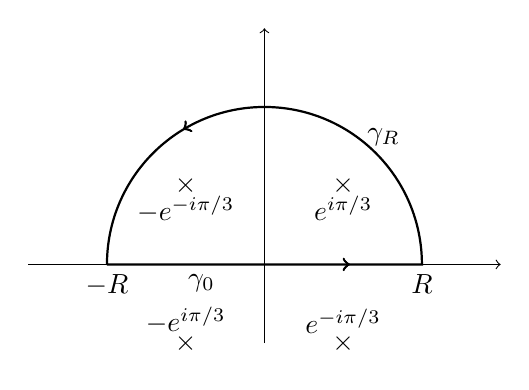
\begin{tikzpicture}
      \draw [->] (-3, 0) -- (3, 0);
      \draw [->] (0, -1) -- (0, 3);

      \draw [black, thick, ->-=0.3, ->-=0.8] (-2, 0) -- (2, 0) node [pos=0.3, below] {$\gamma_0$} arc(0:180:2) node [pos=0.3, right] {$\gamma_R$};

      \node [below] at (-2, 0) {$-R$};
      \node [below] at (2, 0) {$R$};

      \node at (1, 1) {$\times$};
      \node [below] at (1, 1) {$e^{i\pi/3}$};
      \node at (-1, 1) {$\times$};
      \node [below] at (-1, 1) {$-e^{-i\pi/3}$};
      \node at (1, -1) {$\times$};
      \node [above] at (1, -1) {$e^{-i\pi/3}$};
      \node at (-1, -1) {$\times$};
      \node [above] at (-1, -1) {$-e^{i\pi/3}$};
    \end{tikzpicture}
  \end{center}
Only the poles $e^{+i\pi/3}$ and $-e^{-i\pi/3}$ are enclosed. So by residue theorem,
$$\oint_{\gamma_0\cup\gamma_R}g(z)dz=2\pi i\bigg(\frac{e^{i/2}e^{-\sqrt{3}/2}}{-3+i\sqrt{3}}+\frac{e^{-i/2}e^{-\sqrt{3}/2}}{3+i\sqrt{3}}\bigg)=2\pi i\frac{-ie^{-\sqrt{3}/2}}{2}(\sin0.5+3^{-1/2}\cos0.5)$$
The contribution along $\gamma_R:~z=Re^{i\theta},~\theta\in[0,\pi)$ gives $O(R^{-3}e^{-R\cos\theta})\rightarrow0$ as $R\rightarrow\infty$. We have
$$\oint_{\gamma_0\cup\gamma_R}g(z)dz=\int_{-R}^R g(x)dx+\int_{\gamma_R}g(z)dz\rightarrow\int_{-\infty}^\infty g(x)dx+0,\text{ as }R\rightarrow\infty$$
$$\implies\int_{-\infty}^\infty\frac{\cos(x)}{x^4+x^2+1}dx=\text{Re}\bigg[\int_{-\infty}^\infty g(x)dx\bigg]=\pi e^{-\sqrt{3}/2}(\sin 0.5+3^{-1/2}\cos0.5)$$
\end{enumerate}
\end{ans}
\newpage
\begin{qns}[Transform Methods]
The Fourier transform $\tilde{f}(\omega)$ of a function $f(t)$ is defined by
$$\tilde{f}(\omega)=\int_{-\infty}^\infty f(t)e^{-i\omega t}dt$$
\begin{enumerate}[label=(\alph*)]
\item Show that the Fourier transform of $f'(t)$ is given by $i\omega\tilde{f}(\omega)$. Clearly state the assumptions you made about $f(t)$. \hfill\textbf{[2]}
\item Consider the equation for forced damped harmonic motion
$$\frac{d^2y(t)}{dt^2}+2\kappa\frac{dy(t)}{dt}+\Omega^2y(t)=f(t)$$
where $\kappa,\Omega>0$ are given constants and $f(t)$ is a given function.\\[5pt]
Show that $\tilde{y}(\omega)$ can be expressed as $\tilde{y}(\omega)=\tilde{h}(\omega)\tilde{f}(\omega)$, and write down $\tilde{h}(\omega)$.\hfill\textbf{[2]}
\item Show that your expression in (b) can be inverted to find $y(t)$ as
$$y(t)=\int_{-\infty}^\infty G(t-\xi)f(\xi)d\xi$$
where
$$G(t)=\int_{-\infty}^\infty\frac{s(\omega,t)}{(\omega-\omega_-)(\omega-\omega_+)}d\omega$$
for some $\omega_+$, $\omega_-$ and $s(\omega, t)$ that you should determine. The convolution theorem can be used without proof.\hfill\textbf{[3]}
\item Evaluate $G(t)$ for $t > 0$ by closing the contour and using the residue theorem for:\hfill\textbf{[7]}
\begin{itemize}
    \item $\Omega>\kappa$;
    \item $\kappa>\Omega$;
    \item $\kappa=\Omega$.
\end{itemize}
What is the value of $G(t)$ for $t < 0$? Describe the behaviour of $G(t)$ as $t\rightarrow\infty$.\hfill\textbf{[2]}
\item Use your results from parts (c) and (d) to determine $y(t)$ when $f(t) = \cos\kappa t$ and $\Omega=\kappa$.\hfill\textbf{[4]}
\end{enumerate}
\end{qns}
\begin{ans}\leavevmode
\begin{enumerate}[label=(\alph*)]
\item Take Fourier transform of $f'(t)$ is
$$\mathcal{F}[f']=\int_{-\infty}^\infty f'(t)e^{-i\omega t}dt=[fe^{-i\omega t}]_{-\infty}^\infty +i\omega\tilde{f}$$
For $\mathcal{F}[f'(t)]=i\omega\tilde{f}(\omega)$, then we have to assume $f(t)\rightarrow 0$ as $t\rightarrow\pm\infty$.
\item So take the Fourier transform of the forced damped harmonic motion
$$-\omega^2\tilde{y}+2\kappa i\omega\tilde{y}+\Omega^2\tilde{y}=\tilde{f}$$
hence,
$$\tilde{y}=\tilde{f}\tilde{h}\implies\tilde{h}(\omega):=\frac{-1}{\omega^2-2i\kappa\omega-\Omega^2}$$
\item Convolution theorem states $$\tilde{y}(\omega)=\tilde{f}(\omega)\tilde{h}(\omega)\implies y(t)=\int_{-\infty}^\infty f(\xi)h(t-\xi)d\xi$$
Use inverse Fourier transform:
$$y(t)=\int_{-\infty}^\infty\frac{\tilde{y}}{2\pi}e^{i\omega t}d\omega=\frac{-1}{2\pi}\int_{-\infty}^\infty\frac{\tilde{f}e^{i\omega t}d\omega}{\omega^2-2i\kappa\omega-\Omega^2}\implies h(t)=\frac{-1}{2\pi}\int_{-\infty}^\infty\frac{e^{i\omega t}d\omega}{\omega^2-2i\kappa\omega-\Omega^2}$$
This is the Green's function we are looking for with $s(\omega,t)=\frac{-e^{i\omega t}}{2\pi}$ and $\omega_\pm$ are the roots of $\omega^2-2i\kappa\omega-\Omega^2=0\implies\omega_\pm=i\kappa\pm\sqrt{\Omega^2-\kappa^2}$.
\item To evaluate $G$, we consider
$$\oint_C\frac{s(\omega,t)}{(\omega-\omega_-)(\omega-\omega+)}d\omega$$
over a closed loop $C$ in complex $\omega$-plane. The integrand has poles at $\omega_\pm$ with residues (depending on the regime):
\begin{itemize}
    \item $\Omega>\kappa$: $\omega_\pm=i\kappa\pm \sqrt{\Omega^2-\kappa^2}$ are simple poles.
    \begin{align}
        \res_{\omega\rightarrow\omega_\pm}G(t)&=\lim_{\omega\rightarrow\omega_\pm}\frac{1}{\omega-\omega_\mp}\frac{-1}{2\pi}e^{i\omega t}\nonumber\\&=\mp\frac{1}{4\pi\sqrt{\Omega^2-\kappa^2}}e^{-\kappa t}e^{\pm i\sqrt{\Omega^2-\kappa^2}t}\nonumber
    \end{align}
    \item $\Omega<\kappa$: $\omega_\pm=i\kappa\pm i\sqrt{\kappa^2-\Omega^2}$ are simple poles.
    \begin{align}
        \res_{\omega\rightarrow\omega_\pm}G(t)&=\lim_{\omega\rightarrow\omega_\pm}\frac{1}{\omega-\omega_\mp}\frac{-1}{2\pi}e^{i\omega t}\nonumber\\&=\mp\frac{1}{4\pi\sqrt{-\Omega^2+\kappa^2}}e^{-\kappa t}e^{\mp \sqrt{\Omega^2-\kappa^2}t}\nonumber
    \end{align}
    \item $\Omega=\kappa$: $\omega_0=i\kappa$ is a double pole.
    \begin{align}
        \res_{\omega\rightarrow\omega_0}G(t)&=\lim_{\omega\rightarrow\omega_0}\frac{d}{d\omega}\frac{-1}{2\pi}e^{i\omega t}\nonumber\\&=-\frac{it}{2\pi}e^{i\omega t}\nonumber
    \end{align}
\end{itemize}
For $t>0$, we close the upper half-plane (in order to use Jordan's Lemma). Another equivalent explanation:
$$\int_{C_R}\frac{s(\omega)}{(\omega-\omega_-)(\omega-\omega_+)}d\omega=O(R^{-2})\rightarrow0\text{ as }R\rightarrow\infty$$
where $C_R:~z=Re^{i\theta},~\theta\in[0,\pi)$ is a semi-circular arc. Then,
$$\oint_C\frac{s(\omega,t)}{(\omega-\omega_-)(\omega-\omega+)}d\omega=\int_{C_R}\frac{s(\omega)}{(\omega-\omega_-)(\omega-\omega_+)}d\omega+\int_{C_0}\frac{s(\omega)}{(\omega-\omega_-)(\omega-\omega_+)}d\omega\rightarrow G(t)\text{ as } R\rightarrow \infty$$
where $C_R:~z=r,~r\in[-R,R]$. This closed contour $C$ happens to enclose our poles, located in the upper half-plane. Then by residue theorem,
$$\oint_Cf(z)dz=2\pi i\sum_k\res_{z=z_k}f(z)$$
where $f(z)$ is analytic in a simply-connected domain except at a finite number of $k$ isolated singularities, and $C$ is a simple closed contour that traverses in an anti-clockwise fashion.\\[5pt]
For $\Omega>\kappa$, $\sqrt{\Omega^2-\kappa^2}\in\mathbb{R}$ and we have
\begin{center}
    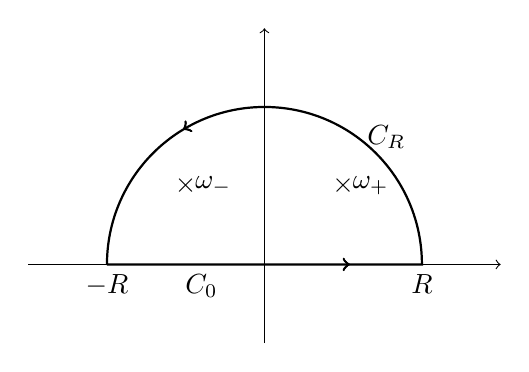
\begin{tikzpicture}
      \draw [->] (-3, 0) -- (3, 0);
      \draw [->] (0, -1) -- (0, 3);

      \draw [black, thick, ->-=0.3, ->-=0.8] (-2, 0) -- (2, 0) node [pos=0.3, below] {$C_0$} arc(0:180:2) node [pos=0.3, right] {$C_R$};

      \node [below] at (-2, 0) {$-R$};
      \node [below] at (2, 0) {$R$};

      \node at (1, 1) {$\times$};
      \node [right] at (1, 1) {$\omega_+$};
      \node at (-1, 1) {$\times$};
      \node [right] at (-1, 1) {$\omega_-$};
    \end{tikzpicture}
  \end{center}
\begin{align}
G(t>0)&=2\pi i\frac{-e^{-\kappa t}}{4\pi\sqrt{\Omega^2-\kappa^2}}(e^{i\sqrt{\Omega^2-\kappa^2}t}-e^{-i\sqrt{\Omega^2-\kappa^2}t})\nonumber\\&=\frac{-2\pi i2i\sin(\sqrt{\Omega^2-\kappa^2}t)e^{-\kappa t}}{4\pi\sqrt{\Omega^2-\kappa^2}}\nonumber\\&=\frac{e^{-\kappa t}}{\sqrt{\Omega^2-\kappa^2}}\sin(\sqrt{\Omega^2-\kappa^2}t)\nonumber
\end{align}
For $\Omega<\kappa$, $\sqrt{\Omega^2-\kappa^2}$ is purely imaginary, and we have
\begin{center}
    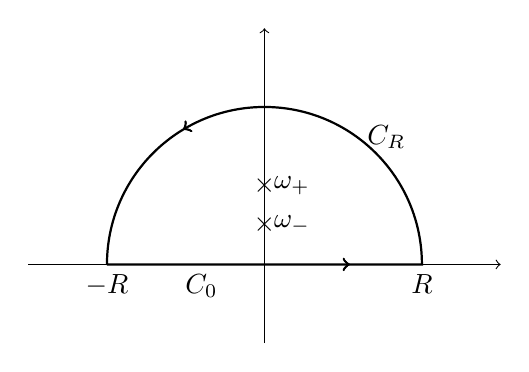
\begin{tikzpicture}
      \draw [->] (-3, 0) -- (3, 0);
      \draw [->] (0, -1) -- (0, 3);

      \draw [black, thick, ->-=0.3, ->-=0.8] (-2, 0) -- (2, 0) node [pos=0.3, below] {$C_0$} arc(0:180:2) node [pos=0.3, right] {$C_R$};

      \node [below] at (-2, 0) {$-R$};
      \node [below] at (2, 0) {$R$};

      \node at (0, 0.5) {$\times$};
      \node [right] at (0, 0.5) {$\omega_-$};
      \node at (0, 1) {$\times$};
      \node [right] at (0, 1) {$\omega_+$};
    \end{tikzpicture}
  \end{center}
\begin{align}
G(t>0)&=2\pi i\frac{-e^{-\kappa t}}{4\pi\sqrt{-\Omega^2+\kappa^2}}(e^{-\sqrt{-\Omega^2+\kappa^2}t}-e^{\sqrt{-\Omega^2+\kappa^2}t})\nonumber\\&=\frac{2\pi i2\sinh(\sqrt{-\Omega^2+\kappa^2}t)e^{-\kappa t}}{4i\pi i\sqrt{-\Omega^2+\kappa^2}}\nonumber\\&=\frac{e^{-\kappa t}}{\sqrt{-\Omega^2+\kappa^2}}\sinh(\sqrt{-\Omega^2+\kappa^2}t)\nonumber
\end{align}
For $\omega=\kappa$, we only have one pole (double pole) on the imaginary axis.
\begin{center}
    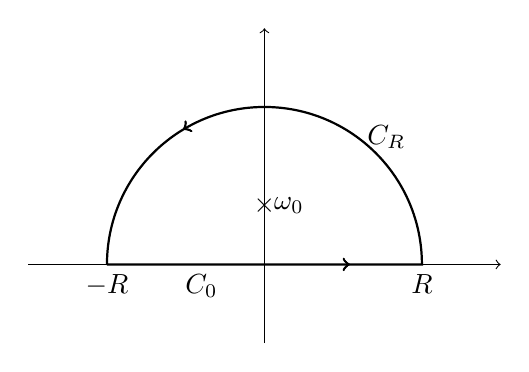
\begin{tikzpicture}
      \draw [->] (-3, 0) -- (3, 0);
      \draw [->] (0, -1) -- (0, 3);

      \draw [black, thick, ->-=0.3, ->-=0.8] (-2, 0) -- (2, 0) node [pos=0.3, below] {$C_0$} arc(0:180:2) node [pos=0.3, right] {$C_R$};

      \node [below] at (-2, 0) {$-R$};
      \node [below] at (2, 0) {$R$};

      \node at (0, 0.75) {$\times$};
      \node [right] at (0, 0.75) {$\omega_0$};
    \end{tikzpicture}
  \end{center}
$$G(t>0)=-2\pi i\frac{it}{2\pi}e^{-\kappa t}=te^{-\kappa t}$$
When $t<0$, we close the lower half-plane, but since there are no poles enclosed, $G(t<0)=0$. This is consistent with causality. As $t\rightarrow\infty$, $e^{-\kappa t}\rightarrow 0$, so $G(t)\rightarrow 0$ regardless of the regime.
\item When $\Omega=\kappa$, $G(t)=te^{-\kappa t}H(t)$ where $H(t)$ is the heaviside function. Rewriting $y(t)$,
\begin{align}
y(t)&=\int_{-\infty}^\infty f(t-\xi)G(\xi)d\xi\nonumber\\&=\int_{-\infty}^\infty\cos(\kappa\xi)(t-\xi)e^{-\kappa(t-\xi)}H(t-\xi)d\xi\nonumber\\&=\int_{-\infty}^\infty\cos(\kappa(t-\xi))\xi e^{-\kappa\xi}d\xi\nonumber\\&=\frac{1}{2}\bigg\{\int_0^\infty\xi e^{-\xi(\kappa+i\kappa)}e^{i\kappa t}d\xi+\int_0^\infty\xi e^{-\xi(\kappa-i\kappa)}e^{-i\kappa t}d\xi\bigg\}\nonumber\\&=\frac{1}{2}\bigg[\frac{e^{i\kappa t}}{(\kappa+i\kappa)^2}+\frac{e^{-i\kappa t}}{(\kappa-i\kappa)^2}\bigg]\nonumber\\&=\frac{\sin\kappa t}{2\kappa^2}\nonumber
\end{align}
where $(\kappa\pm i\kappa)^2=\kappa-\kappa\pm2i\kappa$.
\end{enumerate}
\end{ans}
\begin{qns}[Tensors]\leavevmode
\begin{enumerate}[label=(\alph*)]
\item Show that any second-order tensor $T$ can be written in the form
$$T_{ij} = S_{ij} + \epsilon_{ijk}u_k$$
where $S$ is a symmetric second-order tensor and $\mathbf{u}$ is a vector. Find explicit expressions for $S_{ij}$ and $u_k$ in terms of $T_{ij}$.\hfill\textbf{[5]}
\item Maxwell’s equations for the electric and magnetic fields $\mathbf{E}(\mathbf{x}, t)$ and $\mathbf{B}(\mathbf{x}, t)$ in a vacuum can be written as 
$$\boldsymbol{\nabla}\cdot\mathbf{E}=0,\quad\boldsymbol{\nabla}\cdot\mathbf{B}=0$$
$$\boldsymbol{\nabla}\times\mathbf{E}+\frac{\partial\mathbf{B}}{\partial t}=0,\quad\boldsymbol{\nabla}\times\mathbf{B}-\frac{1}{c^2}\frac{\partial\mathbf{E}}{\partial t}=0$$
where $c$ is a constant. Consider the second-order tensors $T^E_{ij} = \frac{\partial E_j}{\partial x_i}$ and $T^B_{ij} = \frac{\partial B_j}{\partial x_i}$. As in part (a), these can be written in terms of symmetric second-order tensors $S^E$ and $S^B$ and vectors $\mathbf{u^E}$ and $\mathbf{u^B}$, respectively.
\begin{enumerate}[label=(\roman*)]
\item  Calculate expressions for $S^E_{ij}$, $S^B_{ij}$, $\mathbf{u^E}$ and $\mathbf{u^B}$ in terms of $\mathbf{E}$ and $\mathbf{B}$.\hfill\textbf{[2]}
\item Show that\hfill\textbf{[4]}
$$\frac{\partial\mathbf{u^E}}{\partial t}=-\frac{c^2}{2}\nabla^2\mathbf{B}$$
\item Let $V$ denote a constant closed volume with surface $A$. By applying the divergence theorem to a suitable integral expression, show that \hfill\textbf{[4]}
$$\frac{\partial}{\partial t}\int_V(u_i^E+u_i^B)dV=\oint_A(S_{ij}^E-c^2S_{ij}^B)dA_j$$
\item Show further that
$$\frac{\partial}{\partial t}\int_V\lambda dV=\oint_A(\mathbf{B}\times\mathbf{E})\cdot d\mathbf{A}$$
for some scalar quantity $\lambda$ that should be determined in terms of $\mathbf{E}$, $\mathbf{B}$ and $c$.\hfill\textbf{[5]}
\end{enumerate}
\end{enumerate}
\end{qns}
\begin{ans}\leavevmode
\begin{enumerate}[label=(\alph*)]
\item We can decompose a generic second-order tensor:
$$T_{ij}=\frac{1}{2}(T_{ij}+T_{ji})+\frac{1}{2}(T_{ij}-T_{ji})$$
with $S_{ij}=\frac{1}{2}(T_{ij}+T_{ji})$, $A_{ij}=\frac{1}{2}(T_{ij}-T_{ji})=\epsilon_{ijk}u_k$. (anti-symmetric second-order tensor is equivalent to an axial vector). Then,
$$\epsilon_{ijl}A_{ij}=\epsilon_{ijl}\epsilon_{ijk}u_k=(\delta_{jj}\delta_{lk}-\delta_{jk}\delta_{lj})u_k=(3\delta_{lk}-\delta_{lk})u_k=2\delta_{lk}u_k\implies u_k=\frac{1}{2}\epsilon_{ijk}\frac{1}{2}(T_{ij}-T_{ji})$$
\item
\begin{enumerate}[label=(\roman*)]
\item $$S_{ij}^{E}=\frac{1}{2}\bigg(\frac{\partial E_j}{\partial x_i}+\frac{\partial E_i}{\partial x_j}\bigg),~S_{ij}^{B}=\frac{1}{2}\bigg(\frac{\partial B_j}{\partial x_i}+\frac{\partial B_i}{\partial x_j}\bigg),~ u^E_k=\frac{1}{4}\epsilon_{ijk}\bigg(\frac{\partial E_j}{\partial x_i}-\frac{\partial E_i}{\partial x_j}\bigg),~u^B_k=\frac{1}{4}\epsilon_{ijk}\bigg(\frac{\partial B_j}{\partial x_i}-\frac{\partial B_i}{\partial x_j}\bigg)$$
\item Exploit Maxwell's equations, i.e. $\boldsymbol{\nabla}\cdot\mathbf{B}=0$, $\boldsymbol{\nabla}\times\mathbf{B}=\frac{1}{c^2}\frac{\partial\mathbf{E}}{\partial t}$, then
$$\frac{\partial\mathbf{u^E}}{\partial t}=\frac{1}{2}\frac{\partial}{\partial t}\boldsymbol{\nabla}\times\mathbf{E}=\frac{1}{2}\boldsymbol{\nabla}\times c^2(\boldsymbol{\nabla}\times\mathbf{B})=-\frac{c^2}{2}\nabla^2\mathbf{B}$$
\item Apply Divergence theorem to $(S^E-c^2S^B)\mathbf{v}$ where $\mathbf{v}$ is an arbitrary constant vector.
\begin{align}
    \int_V\boldsymbol{\nabla}\cdot[(S^E-c^2S^B)\mathbf{v}]dV&=\oint_A(S^E-c^2S^B)\mathbf{v}\cdot d\mathbf{A}\nonumber\\\implies\int_V\frac{\partial}{\partial x_j}(S_{ij}^E-c^2S_{ij}^B)v_idV=&=\oint_A(S_{ij}^E-c^2S_{ij}^B)v_idA_j\nonumber
\end{align}
but $\mathbf{v}$ is constant so we can pull it out of the integral. $\mathbf{v}$ is arbitrary so we can just equate the coefficients. 
\begin{align}
    \oint_A(S_{ij}^E-c^2S_{ij}^B)dA_j&=\frac{1}{2}\int_V\frac{\partial^2E_i}{\partial x_j\partial x_j}+\frac{\partial E_j}{\partial x_i\partial x_j}-c^2\frac{\partial^2B_i}{\partial x_j\partial x_j}-c^2\frac{\partial^2B_j}{\partial x_i\partial x_j}dV\nonumber\\&=\frac{1}{2}\int_V2\frac{\partial u^B}{\partial t}+0-\frac{c^2}{c^2}2\frac{\partial u_i^E}{|partial t}-0dV\nonumber\\&=\frac{\partial}{\partial t}\int_Vu_i^B+u_i^EdV\nonumber
\end{align}
\item Apply Divergence theorem to $\mathbf{B}\times\mathbf{E}$, noting that
$$\boldsymbol{\nabla}\cdot(\mathbf{E}\times\mathbf{B})=\partial_i(\epsilon_{ijk}E_jB_k)=\epsilon_{ijk}(\partial_iE_j)B_k+\epsilon_{ijk}(\partial_iB_k)E_j=\mathbf{B}\cdot(\boldsymbol{\nabla}\times\mathbf{E})-\mathbf{E}\cdot(\boldsymbol{\nabla}\times\mathbf{B})$$
Together with the Maxwell equations $\frac{\partial\mathbf{B}}{\partial t}=-\boldsymbol{\nabla}\times\mathbf{E}$ and $\frac{\partial\mathbf{E}}{\partial t}=c^2\boldsymbol{\nabla}\times\mathbf{B}$:
$$\int_V\boldsymbol{\nabla}\cdot(\mathbf{E}\times\mathbf{B})dV=
\int\mathbf{E}\cdot(\boldsymbol{\nabla}\times\mathbf{B})-\mathbf{B}\cdot(\boldsymbol{\nabla}\times\mathbf{E})dV=\int\frac{\partial\mathbf{E}}{\partial t}\cdot\mathbf{E}+\frac{\partial\mathbf{B}}{\partial t}\cdot\mathbf{B}dV$$
But this is $-\frac{\partial}{\partial t}\int_V\lambda dV$ and hence $\lambda=-\frac{1}{2}(\mathbf{B}\cdot\mathbf{B}+\frac{1}{c^2}\mathbf{E}\cdot\mathbf{E})$.
\end{enumerate}
\end{enumerate}
\end{ans}
\begin{qns}[Normal Modes]\leavevmode
\begin{enumerate}[label=(\alph*)]
\item Write down a general Lagrangian of a system with $n$ degrees of freedom undergoing small oscillations, and state the polynomial equation for the normal frequencies.\hfill\textbf{[5]}
\item A simple pendulum of mass $M$ and length $L$ is suspended from a cart of mass $m$ that can oscillate on the end of a spring of force constant $k$, as shown in the figure. The cart is constrained to move in the horizontal direction only, and has a displacement $x(t)$ from its equilibrium position. The pendulum oscillates in the plane making angle $\phi(t)$ with the vertical direction.
\begin{figure}[H]
    \centering
    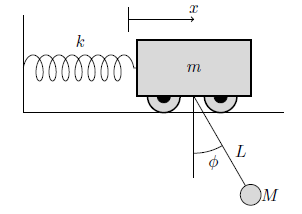
\includegraphics[scale=0.95]{2018P2Q7.PNG}
\end{figure}
\begin{enumerate}[label=(\roman*)]
\item Assuming that the angle $\phi$ and displacement $x$ remain small, write down the system’s Lagrangian and the equations of motion for $x$ and $\phi$. \hfill\textbf{[8]}
\item Assuming that $m = M = L = g = 1$ and $k = 2$ (all in appropriate units), where $g$ is the constant acceleration due to gravity, find the normal frequencies. For each normal frequency, find and describe the motion of the corresponding normal mode.
\end{enumerate}
\end{enumerate}
\end{qns}
\newpage
\begin{ans}\leavevmode
\begin{enumerate}[label=(\alph*)]
\item If the coordinates of the $n$ degrees of freedom are $q_i$ with corresponding velocities $\dot{q}_i$, and we keep only quadratic terms in the Lagrangian, we have
$$\mathcal{L}=\frac{1}{2}\dot{q}^TM\dot{q}-\frac{1}{2}q^TKq$$
where the linear terms vanish due to expanding about equilibrium, and we have dropped the irrelevant constant term. Also we have restricted to velocity-independent potentials. Here, we can just take the symmetric parts of the second-order tensors $M$ and $K$. The corresponding characteristic polynomial equation for the normal frequencies $\omega_j$ is
$$\det(K-\omega^2M)=0$$
\item 
\begin{enumerate}[label=(\roman*)]
\item We have $X(t)=x(t)+L\sin\phi$ and $Y(t)=L(1-\cos\phi)$, where we let $x(t)=0$ be vertically underneath the cart. The Lagrangian is
\begin{align}
    \mathcal{L}&=\frac{1}{2}m\dot{x}^2+\frac{1}{2}M(\dot{X}^2+\dot{Y}^2)-\frac{1}{2}kx^2-Mgy\nonumber\\&=\frac{1}{2}m\dot{x}^2+\frac{1}{2}M(\dot{x}+2L\cos\phi\dot{x}\dot{\phi}+L^2\cos^2\phi\dot{\phi}^2+L^2\sin^2\phi\dot{\phi}^2)-\frac{1}{2}kx^2-MgL(1-\cos\phi)\nonumber\\&=\frac{1}{2}(m+M)\dot{x}^2+\frac{1}{2}m(L^2\dot{\phi}^2+2L\dot{x}\dot{\phi})-\frac{1}{2}kx^2-\frac{1}{2}MgL\phi^2\nonumber\\&=\frac{1}{2}\begin{pmatrix}\dot{x}&\dot{\phi}\\\end{pmatrix}\begin{pmatrix}m+M&ML\\ML&L^2\\\end{pmatrix}\begin{pmatrix}\dot{x}\\\dot{\phi}\\\end{pmatrix}-\frac{1}{2}\begin{pmatrix}x&\phi\\\end{pmatrix}\begin{pmatrix}k&0\\0&MgL\\\end{pmatrix}\begin{pmatrix}x\\\phi\\\end{pmatrix}\nonumber
\end{align}
The corresponding equations of motion (use Euler-Lagrange equations to extremize the Lagrangian) is a system of ODE:
\begin{align}
0&=\frac{d}{dt}\frac{\partial\mathcal{L}}{\partial\dot{q}}-\frac{\partial\mathcal{L}}{\partial\mathbf{q}}\nonumber\\&=\frac{d}{dt}\begin{pmatrix}m+M&ML\\ML&L^2\\\end{pmatrix}\begin{pmatrix}\dot{x}\\\dot{\phi}\\\end{pmatrix}+\begin{pmatrix}k&0\\0&MgL\\\end{pmatrix}\begin{pmatrix}x\\\phi\\\end{pmatrix}\nonumber
\end{align}
\item The matrix equation (equation of motion) is now
$$0=\frac{d}{dt}\begin{pmatrix}2&1\\1&1\\\end{pmatrix}\begin{pmatrix}\dot{x}\\\dot{\phi}\\\end{pmatrix}+\begin{pmatrix}2&0\\0&1\\\end{pmatrix}\begin{pmatrix}x\\\phi\\\end{pmatrix}$$
Hence, the characteristic polynomial gives
$$0=\det\begin{pmatrix}2-2\omega^2&-\omega^2\\-\omega^2&1-\omega^2\\\end{pmatrix}=2(1-\omega^2)^2-\omega^2\implies\omega^2=\frac{\sqrt{2}}{\sqrt{2}\pm 1}=2\mp\sqrt{2}$$
Plug these normal frequencies back to the system of linear equations:
$$\boldsymbol{0}=\begin{pmatrix}2-2(2\pm\sqrt{2})&-(2\pm\sqrt{2})\\-(2\pm\sqrt{2})&1-(2\pm\sqrt{2})\\\end{pmatrix}\begin{pmatrix}a_\pm\\b_\pm\\\end{pmatrix}$$
which gives the eigenvectors $(\mp1,\sqrt{2})^T$ for the normal frequencies $\sqrt{2\pm\sqrt{2}}$ respectively (anti-phase and in-phase respectively).
\end{enumerate}
\end{enumerate}
\end{ans}
\newpage
\begin{qns}[Group Theory]\leavevmode
\begin{enumerate}[label=(\alph*)]
\item  Let $G$, $G'$ be two finite groups and let $f : G\rightarrow G'$ be a group homomorphism. Let $a\in G$. Show that the order of $f(a)$ is at most the order of $a$. Show that if $f$ is an isomorphism then $a$ and $f(a)$ have the same order.\hfill\textbf{[6]}
\item If $a,b\in G$ show that $ab$ and $ba$ have the same order.\hfill\textbf{[7]}
\item Let $G$ be a finite group where the order of each element is at most 2. Show that $G$ is abelian.

\hfill\textbf{[7]}
\end{enumerate}
\end{qns}
\begin{ans}\leavevmode
\begin{enumerate}[label=(\alph*)]
\item Let the order of $a\in G$ be $\ord(a)$, then $a^{\ord(a)}=e$, the identity of $G$. Let $f:~G\rightarrow G'$ be a homomorphism, then for $a_1,a_2\in G$,
$$f(a_1)f(a_2)=f(a_1a_2)$$
Suppose $f(a)$ has order $p<\ord(a)$, then $e=[f(a)]^p=f(a^p)$ where we used the fact that $f$ is a homomorphism. This is possible since $f$ is not specified to be injective, so $e$ is not the unique element that maps to $e$.\\[5pt]
Suppose $f(a)$ has order $\ord(a)+1$, then
$$e=(f(a))^{\ord(a)+1}=f(a)(f(a))^{\ord(a)}=f(a)[f(a^{\ord(a)}]=f(a)f(e)=f(a)$$
This contradicts since $\ord(a)+1$ is constructed to be the smallest positive integer power for $f(a)$ to be raised to obtain the identity. But we found a smaller integer, i.e. 1. So, $f(a)$ must have order at most $\ord(a)$.\\[5pt]
If $f$ is an isomorphism, it must be injective, so $f(a^p)=e$ is not allowed, and so for $[f(a)]^p=e$, $p=\ord(a)$.
\item Let the order of $ab$ be $r$, then
$$e=(ab)^r=(ab)^raa^{-1}=a(ba)^ra^{-1}\implies(ba)^r=a^{-1}ea=e$$
so the order of $ba$ is $r=\ord(ab)$.
\item For $g\in G$ and $g\neq e$, then $\ord(g)$ is specified to be 2. Consider such $g_1,g_2\in G$ where $g_1\neq g_2$, then
$$e=g_1^2=g_2^2$$
Consider $g_1g_2$
$$g_1g_2=g_2^2g_1g_2g_1^2=g_2(g_2g_1)^2g_1=g_2g_1$$
Hence, $G$ is abelian.
\end{enumerate}
\end{ans}
\newpage
\begin{qns}[Group Theory]\leavevmode
\begin{enumerate}[label=(\alph*)]
\item Let $G$ be a group, and $H_1$ and $H_2$ two subgroups of $G$. Show that the claims (I) and (II) below are equivalent.\hfill\textbf{[10]}
\begin{enumerate}[label=\Roman*.]
    \item $H_1\cap H_2 = \{1\}$ and any element $g\in G$ can be written as $g = h_1h_2$, where $h_1\in H_1$ and $h_2\in H_2$.
    \item Any element $g\in G$ can be written in a unique way as $g = h_1h_2$ where $h_1\in H_1$ and $h_2\in H_2$.
\end{enumerate}
\item Let $H_1$ be the group of matrices generated by $\bigg\{\begin{pmatrix}-1&0\\0&1\\\end{pmatrix},\begin{pmatrix}1&0\\0&-1\\\end{pmatrix}\bigg\}$ and let $H_2$ be the (cyclic) group generated by the single matrix $\begin{pmatrix}0&1\\1&0\\\end{pmatrix}$. Also let $G$ be the smallest group containing $H_1$ and $H_2$. How many elements does $G$ have? \hfill\textbf{[5]}\\[5pt]
Show that $G$, $H_1$ and $H_2$ satisfy the condition (I).\hfill\textbf{[5]}
\end{enumerate}
\end{qns}

\begin{ans}\leavevmode
\begin{enumerate}[label=(\alph*)]
\item Consider the direct product group $H_1\times H_2$ and the function
\begin{eqnarray}
\phi: H_1\times H_2&\rightarrow&G\nonumber\\(h_1,h_2)&\mapsto& h_1\cdot h_2\nonumber
\end{eqnarray}
where $h_1\in H_1$ and $h_2\in H_2$. We want to show if $H_1\cap H_2=\{1\}$, then $\phi$ is an isomorphism such that $(h_1,h_2)$ is mapped to a unique element $h_1h_2\in G$. Firstly, check that $\phi$ is a homomorphism:
$$\phi((h_1,h_2)\cdot(h_1',h_2'))=\phi((h_1h_1',h_2h_2'))=h_1h_1'h_2h_2'=h_1h_2h_1'h_2'=\phi((h_1,h_2))\phi((h_1',h_2'))$$
Given for each $g\in G$, $\exists h_1\in H_1$, $h_2\in H_2$ s.t. $g=h_1h_2$, then $\phi$ is surjective. If $\phi((h_1,h_2))=1$, then $h_1h_2=1$, and so $h_1=h_2^{-1}\in H_1,H_2$, so if $H_1\cap H_2=\{1\}$, then $1\in H_1,H_2$. Hence, $(h_1,h_2)=(1,1)\in\Ker\phi$ (this homomorphism has trivial kernel) and so $\phi$ is an isomorphism.\\[5pt]
Conversely, if we can show $g=h_1h_2$ is a unique decomposition, then there is a bijective mapping between $G$ and $H_1\times H_2$. Since we can construct an isomorphism, the kernel of this bijective mapping is trivial, and so $(1,1)\in\Ker\phi\implies H_1\cap H_2=\{1\}$.
\item Let the corresponding groups generated be
$$H_1=\bigg\{\begin{pmatrix}1&0\\0&1\\\end{pmatrix},\begin{pmatrix}-1&0\\0&1\\\end{pmatrix},\begin{pmatrix}1&0\\0&-1\\\end{pmatrix},-\begin{pmatrix}1&0\\0&1\\\end{pmatrix}\bigg\}:=\{e,a,b,ab\}$$
$$H_2=\bigg\{\begin{pmatrix}1&0\\0&1\\\end{pmatrix},\begin{pmatrix}0&1\\1&0\\\end{pmatrix}\bigg\}:=\{e,c\}$$
where $\ord(a)=\ord(b)=\ord(ab)=\ord(c)=2$. Note $a$ and $b$ commute but not $a$ and $c$ or $b$ and $c$. The smallest group $G$ containing $H_1$ and $H_2$ is 
$$G=\{e,a,b,ab,c,ac,bc,abc\}$$
with group table:
$$\vbox{\tabskip0.5em\offinterlineskip
    \halign{\strut$#$\hfil\ \tabskip1em\vrule&&$#$\hfil\cr
    ~&e&a&b&ab & c & ac & bc & abc   \cr
    \noalign{\hrule}\vrule height 12pt width 0pt
     e&e&a&b&ab & c & ac & bc & abc   \cr
     a & a& e&ab& b&ac&c&abc&bc \cr
     b & b &ab&e&a&bc&abc&c&ac \cr
     ab & ab&b&a&e&abc&bc&ac&c\cr
     c & c & ac & bc & abc & e & a &b & ab \cr
     ac & ac & c & abc & bc & a & ab & e & b \cr
     bc & bc & c & abc & ac & b & e &ab &a \cr
     abc & abc & bc & ac & c & ab & a & b &e \cr
}}$$
where we have the following identities: $ab=ba$, $ac=cb=-bc$ and $bc=ca=-ac$. Check group axioms:
\begin{itemize}
    \item closure: the rows of the group table are identical up to permutations.
    \item associative: matrix multiplication is associative.
    \item identity: $e\in G$.
    \item inverse: $a$, $b$, $ab$, $c$ and $abc$ are their own self-inverse, while $(ac)^{-1}=bc$.
\end{itemize}
So $G$ is a group and $|G|=8$.\\[5pt]
Obvious $H_1\cap H_2$ is the identity matrix. For $G$ to be closed and since $G$ contains $H_1$ and $H_2$, then $g=h_1h_2$ for some $h_1\in H_1$ and $h_2\in H_2$, thus satisfying (I). Note that (II) is not satisfied since $h_1h_2\neq h_2h_1$ (non-unique decomposition).
\end{enumerate}
\end{ans}
\begin{qns}[Representation Theory]\leavevmode
\begin{enumerate}[label=(\alph*)]
\item Let $D$ be a representation of $G$; i.e. a homomorphism $D : G\rightarrow \text{GL}(n,\mathbb{C})$, where $\text{GL}(n,\mathbb{C})$ is the group of $n\times n$ invertible complex matrices. What does it mean for a vector subspace $W\subset\mathbb{C}^n$ to be an invariant subspace with respect to $D$? What does it mean for $D$ to be irreducible?\hfill\textbf{[4]}
\item Let $D_1 : G \rightarrow\text{GL}(n,\mathbb{C})$ be a representation, and define 
$$D_2(g) = [D_1(g^{−1})]^\dag$$
where $\dag$ denotes the hermitian conjugate. Show that $D_2$ is a representation.\hfill\textbf{[6]}
\item Suppose that $W$ is an invariant subspace of $\mathbb{C}^n$ with respect to $D_2$. Show that $W_\perp$ is an invariant subspace of $\mathbb{C}^n$ with respect to $D_1$, where $W_\perp$ is the vector space of vectors orthogonal to $W$. Hence show that if $D_1$ is irreducible then $D_2$ must also be irreducible.\hfill\textbf{[10]}
\end{enumerate}
\end{qns}
\begin{ans}\leavevmode
\begin{enumerate}[label=(\alph*)]
\item $W\subset\mathbb{C}^n$ is said to be an invariant subspace with respect to the representation $D$ if for any vector $w\in W$,
$$D(g)(w)\in W\subset\mathbb{C}^n\quad\forall g\in G$$
If $D$ is irreducible, then $D$ has no non-trivial invariant subspaces (trivial subspaces are the nullspace and the entire vector space), and the matrices of $D$ cannot be transformed into block-diagonal form.
\item For $D_2$ to be a representation, it must be a homomorphism. For $g_1,g_2\in G$, then
$$D_2(g_1)D_2(g_2)=[D_1(g_1^{-1})]^\dag[D_1(g_2^{-1})]^\dag=[D_1(g_2^{-1})D_1(g_1^{-1})]^\dag=[D_1(g_2^{-1}g_1^{-1})]^\dag=D_2(g_1g_2)$$
\item Suppose $W$ is an invariant subspace of $\mathbb{C}^n$ with respect to $D_2$, then
$$D_2(g)(w)\in W\quad\forall w\in W,~\forall g\in G$$
Then $\forall y\in W_\perp$, we must have
$(D_2(g)(w))^\dag y=0$ (inner product) since $D_2(g)(w)\in W$. 
$$0=w^\dag D_2(g)^\dag y=w^\dag D_1(g{-1})y\implies D_1(g^{-1}y)\in W_\perp$$
Hence, $W_\perp$ is an invariant subspace with respect to $D_1$. If $D_1$ is irreducible, $D_1$ has no invariant subspaces. There will then be no subspaces orthogonal to them and so $D_2$ is irreducible.
\end{enumerate}
\end{ans}
\newpage
\section{2019}
\subsection{Paper 1}
\begin{qns}[Vector Calculus]\leavevmode
\begin{enumerate}[label=(\alph*)]
    \item For vector fields $\mathbf{A}$ and $\mathbf{B}$ in three dimensions, show that\hfill\textbf{[3]}
$$\boldsymbol{\nabla}\times(\mathbf{A}\times\mathbf{B})=(\mathbf{B}\cdot\boldsymbol{\nabla})\mathbf{A}-\mathbf{B}(\boldsymbol{\nabla}\cdot\mathbf{A})-(\mathbf{A}\cdot\boldsymbol{\nabla})\mathbf{B}+\mathbf{A}(\boldsymbol{\nabla}\cdot\mathbf{B})$$
\item State Stokes’s theorem, taking care to define all the quantities which appear. \hfill\textbf{[2]}
\item Elliptic cylindrical coordinates $(u, v, z)$ are related to Cartesian coordinates $(x, y, z)$ by
$$x = a \cosh u \cos v,\quad y = a \sinh u \sin v,\quad z = z$$
where $u > 0$, $0\leq v<2\pi$, $-\infty<z<\infty$, and $a$ is a positive real constant. Find the basis vectors $\mathbf{h_u}$, $\mathbf{h_v}$ and $\mathbf{h_z}$ defined by $d\mathbf{r} = \mathbf{h_u} du + \mathbf{h_v} dv + \mathbf{h_z} dz$, show that the coordinates are orthogonal, and find the scale factors $h_u$, $h_v$ and $h_z$.\hfill\textbf{[5]}
\item Describe the surfaces of constant $u$, the surfaces of constant $v$ and the surfaces of constant $z$.\hfill\textbf{[3]}
\item Consider the surface $S$ with $z = c$ and
$$\frac{x^2}{\cosh^21}+\frac{y^2}{\sinh^21}\leq a^2$$
where $c$ is a positive constant and the normal to $S$ points in the positive $z$ direction. Calculate 
$$\int_S(\boldsymbol{\nabla}\times\mathbf{F})\cdot d\mathbf{S}$$
where $\mathbf{F} = (2 \sinh u \sin v,−2 \cosh u \cos v, \cosh u)$ in Cartesian coordinates. \hfill\textbf{[7]}
\end{enumerate}
\end{qns}
\begin{ans}\leavevmode
\begin{enumerate}[label=(\alph*)]
    \item Use suffix notation in Cartesian coordinates to evaluate $\boldsymbol{\nabla}\times(\mathbf{A}\times\mathbf{B})$:
$$\epsilon_{ijk}\frac{\partial}{\partial x_i}\epsilon_{pqj}A_pB_q\mathbf{\hat{k}}=(\delta_{kp}\delta_{iq}-\delta_{kq}\delta_{ip})\bigg(\frac{\partial A_p}{\partial x_i}B_q+\frac{\partial B_q}{\partial x_i}A_p\bigg)\mathbf{\hat{k}}=\bigg(\frac{\partial A_k}{\partial x_i}B_i+\frac{\partial B_i}{\partial x_i}A_k-\frac{\partial A_i}{\partial x_i}B_k-\frac{\partial B_k}{\partial x_i}A_i\bigg)\mathbf{\hat{k}}$$
\item Let $\mathbf{F}=\mathbf{F}(\mathbf{x})$ be a continuously differentiable vector field, and let surface $S$ be orientable, piecewise regular with piecewise smooth boundary $\partial S$, then the Stokes' theorem states that $\int_S(\boldsymbol{\nabla}\times\mathbf{F})\cdot d\mathbf{S}=\oint_{\partial S}\mathbf{F}\cdot d\mathbf{x}$.
\item $\mathbf{h_u}=\frac{\partial\mathbf{r}}{\partial u}=(a\sinh u\cos v,a\cosh u\sin v,0)^T$, $\mathbf{h_v}=\frac{\partial\mathbf{r}}{\partial v}=(-a\cosh u\sin v,a\sinh u\ cos v,0)^T$, $\mathbf{h_z}=\frac{\partial\mathbf{r}}{\partial z}=(0,0,1)^T$, where $d\mathbf{r}=\mathbf{h_u}du+\mathbf{h_v}dv+\mathbf{h_z}dz$. We have $h_u=a^2(\sinh^2u\cos^2v+\cosh^2u\sin^2v)=h_v$, $h_z=1$. We can show $\mathbf{h_u}\cdot\mathbf{h_v}=0$, $\mathbf{h_u}\cdot\mathbf{h_z}=\mathbf{h_v}\cdot\mathbf{h_z}=0$, hence $\{\mathbf{h_u},\mathbf{h_v},\mathbf{h_z}\}$ is an orthogonal set.
\item For constant $u$ and constant $v$, we have
$$1=\cos^2v+\sin^2v=\bigg(\frac{x}{a\cosh u}\bigg)^2+\bigg(\frac{y}{a\sinh u}\bigg)^2,\quad 1=\cosh^2u-\sinh^2u=\bigg(\frac{x}{a\cos v}\bigg)^2-\bigg(\frac{y}{a\sin v}\bigg)^2$$
which are respectively an elliptical cylinder, centred on the $z$-axis of semi-axes $a\cosh u$ and $a\sinh u$ and a hyperbolic cylinder, centred on the $z$-axis. For constant $z$, we have horizontal planes at height $z=c$.
\item Surface $S$ has $z=c$, $\frac{x^2}{\cosh^2(1)}+\frac{y^2}{\sinh^2(1)}\leq a^2\implies u=1$. Use Stokes' Theorem, $C$ is the cross-section in the ellipse in the $z=c$ plane, then
$$\int_S(\boldsymbol{\nabla}\times\mathbf{F})\cdot d\mathbf{S}=\oint_C\mathbf{F}\cdot d\mathbf{l}=\int_0^{2\pi}(-2\sinh(1)\cosh(1)a)(\cos^2v+\sin^2v)dv=-2\pi a \sinh(2)$$
\end{enumerate}
\end{ans}
\begin{qns}[Partial Differential Equation]
The temperature, $T(x, y, t)$, in a two-dimensional bar satisfies
$$\frac{1}{\lambda}\frac{\partial T}{\partial t}=\bigg(\frac{\partial^2T}{\partial x^2}+\frac{\partial^2T}{\partial y^2}\bigg)$$
where $0\leq x\leq a$, $0\leq y\leq b$ and $\lambda$ is a positive constant. The sides $x = 0$ and $x = a$ are held at fixed temperature $T = 0$, whereas the sides $y = 0$ and $y = b$ are insulating, i.e. $\frac{\partial T}{\partial y}|_{y=0}=\frac{\partial T}{\partial y}|_{y=b}=0$. \begin{enumerate}[label=(\alph*)]
\item Using separation of variables and carefully explaining your working, show that the general solution can be written as
$$T(x,y,t)=\sum_{n,m}A_{mn}\sin\bigg(\frac{n\pi x}{a}\bigg)\cos\bigg(\frac{m\pi y}{b}\bigg)\exp\bigg[-\bigg(\frac{n^2}{a^2}+\frac{m^2}{b^2}\bigg)\pi^2\lambda t\bigg]$$
where $A_{nm}$ are constants and you should specify the ranges of $n$ and $m$ in the sum. \hfill\textbf{[8]}\item The initial temperature is $T(x,y,0)=x(a-x)\sin^2(\frac{2\pi y}{b})$. What is $T(x, y, t)$?\hfill\textbf{[10]}
\item What is the leading term in $T(x, y, t)$ for large $t$?\hfill\textbf{[2]}
\end{enumerate}
\end{qns}
\begin{ans}\leavevmode
\begin{enumerate}[label=(\alph*)]
\item  Since the boundary conditions are homogeneous, we use separation of variables $T(x,y,t)=X(x)Y(y)\tau(t)$. We have
$$\frac{1}{\lambda}\frac{\tau'}{\tau}=\frac{X''}{X}+\frac{Y''}{Y}=-\mu$$
we further define $\frac{X''}{X}=-\omega^2$. Since $T(0,y,t)=T(a,y,t)=0$, $\omega=\frac{n\pi}{a}$ and so $X(x)\sim\sin\frac{n\pi x}{a}$. Since $\frac{\partial T}{\partial y}(x,0,t)=\frac{\partial T}{\partial y}(x,b,t)=0$, $Y(y)\sim\cos\frac{m\pi y}{b}$. Hence, $\mu=\pi^2(\frac{m^2}{b^2}+\frac{n^2}{a^2})$ and so $\tau(t)\sim e^{-\mu\lambda t}$. The general solution will be
$$T(x,y,t)=\sum_{n,m}A_{mn}\sin\frac{n\pi x}{a}\cos\frac{m\pi y}{b}e^{-(\frac{n^2}{a^2}+\frac{m^2}{b^2})\pi^2\lambda t}$$
\item The initial condition is
$$x(a-x)\sin^2\frac{2\pi y}{b}=T(x,y,0)=\sum_{n,m}A_{mn}\sin\frac{n\pi x}{a}\cos\frac{m\pi y}{b}$$
Write $\sin^2\frac{2\pi y}{b}=\frac{1}{2}(1-\cos\frac{4\pi y}{b})$, then using Fourier series,
$$\frac{1}{2}(1-\cos\frac{4\pi y}{b})\int_0^a(ax-x^2)\sin\frac{p\pi x}{a}dx=\sum_{n=1}^\infty\sum_{m=0}^\infty A_{mn}\cos\frac{m\pi y}{b}\int_0^a\sin\frac{n\pi x}{a}\sin\frac{p\pi x}{a}dx$$
We have $\int(ax-x^2)\sin\nu xdx=a(-\nu^{-1}x\cos\nu x+\nu^{-2}\sin\nu x)+\nu^{-1}x^2\cos\nu x-2x\nu^{-2}\sin\nu x-2\nu^{-3}\cos\nu x$ and $\int_0^a\sin\frac{n\pi x}{a}\sin\frac{p\pi x}{a}dx=\frac{a}{2}\delta_{n,p}$, and thus
$$\frac{1}{2}(1-\cos\frac{4\pi y}{b})\frac{2a^3}{p^3\pi^3}[1-(-1)^p]=\frac{a}{2}\sum_{m=0}^\infty A_{mp}\cos\frac{m\pi y}{b}$$
Doing it again, but it is obvious only $A_{0p}=A_{4p}\neq 0$. Set $p=2r-1$, then
$$T(x,y,t)=\sum_{r=1}^\infty\frac{4a^3}{(2r-1)^3\pi^3}\sin\frac{(2r-1)\pi x}{a}\bigg(1-\cos\frac{4\pi y}{b}e^{-16\pi^2\lambda t/b^2}\bigg)e^{-(2r-1)^2\pi^2\lambda t/a^2}$$
\item When $t>>1$, the $r=1$ term dominates, and so $T(x,y,t)\approx e^{-\pi^2\lambda t/a^2}\frac{4a^3}{\pi^3}\sin\frac{\pi x}{a}$.
\end{enumerate}
\end{ans}
\newpage
\begin{qns}[Green's Functions]\leavevmode
\begin{enumerate}[label=(\alph*)]
\item  Consider an inhomogeneous ordinary differential equation of the form
\begin{equation}
    y''(x)+p(x)y'(x)+q(x)y(x)=f(x)\tag{*}
\end{equation}
for $a\leq x\leq b$ subject to homogeneous boundary conditions at $x = a$ and $b$. Suppose that $y_a(x)$ and $y_b(x)$ are linearly independent solutions of the homogeneous equation (where $f(x) = 0$) and satisfy the boundary conditions at $x = a$ and $x = b$ respectively. Show that the Green’s function can be written as
$$G(x,z)=
\left\{
        \begin{array}{ll}
      \frac{y_a(x)y_b(z)}{W(z)} & a\leq x< z \\
      \frac{y_b(x)y_a(z)}{W(z)} & z< x\leq b 
        \end{array}
    \right.$$
where $W(z)=y_a(z)y_b'(z)-y_b(z)y_a'(z)$. \hfill\textbf{[5]}
\item Write an expression for $y(x)$, the solution of (*), in terms of an integral involving $f$ and $G$.

\hfill\textbf{[1]}
\item  Find the general solution $y(x)$ of
$$\frac{d^2y}{dx^2}-\frac{3}{x}\frac{dy}{dx}+3\frac{y}{x^2}=0$$
[Hint: Consider $y = x^n$.] \hfill\textbf{[3]}
\item Consider the equation
$$\frac{d^2y}{dx^2}-\frac{3}{x}\frac{dy}{dx}+3\frac{y}{x^2}=f(x)$$
for $0\leq x\leq 1$, with boundary conditions $y(0) = y(1) = 0$.
\begin{enumerate}[label=(\roman*)]
\item Find the Green’s function, $G(x, z)$. \hfill\textbf{[3]}
\item Find $y(x)$ when \hfill\textbf{[8]}
$$f(x)=
\left\{
        \begin{array}{ll}
      0 & 0\leq x\leq 0.5 \\
      x^2 & 0.5\leq x\le1 
        \end{array}
    \right.$$
    \end{enumerate}
\end{enumerate}
\end{qns}
\begin{ans}\leavevmode
\begin{enumerate}[label=(\alph*)]
\item  The corresponding Green's function satisfy
$$\frac{\partial^2G(x,z)}{\partial x^2}+p(x)\frac{\partial G(x,z)}{\partial x}+q(x)G(x,z)=\delta(x-z),\quad G(a,z)=G(b,z)=0$$
We choose the linearly independent homogeneous solutions $y_a$ and $y_b$ such that $y_a(a)=0$ and $y_b(b)=0$. Whenever $x\neq z$, we can write $G(x,z)$ as a linear combination of $y_a(x)$ and $y_b(x)$, i.e.
$$G(x,z)=
\left\{
        \begin{array}{ll}
      A(z)y_a(x)+B(z)y_b(x) & a\leq x<z<b \\
      C(z)y_a(x)+D(z)y_b(x) & z<x\leq b
        \end{array}
    \right.$$
$G(x=a,z)=0\implies 0=A(z)y_a(a)+B(z)y_b(a)\implies B(z)=0$ and $G(x=b,z)=0\implies 0=C(z)y_a(b)+D(z)y_b(b)\implies C(z)=0$. Integrate over an infinitesimal region from $x=\mu$ to $x=\mu+\epsilon$, we get
$$\bigg[\frac{\partial G}{\partial x}\bigg]_\mu^{\mu+\epsilon}+p(\mu)[G]_{\mu}^{\mu+\epsilon}+q(\mu)G(\mu,z)\epsilon=\delta(\mu-z)$$
Take $\epsilon\rightarrow 0$, $G$ is continuous at $x=z$ ($G$ should be continuous everywhere otherwise $G''\propto\delta'(x-z)$ which is a contradiction) and $\frac{\partial G}{\partial x}$ is discontinuous at $x=z$ (unit jump). The continuity and jump conditions respectively give 
$$A(z)y_a(z)=D(z)y_b(z)$$ 
$$D(z)y_b'(z)-A(z)y_a'(z)=1$$
\begin{align}
\begin{pmatrix}y_a(z)&-y_b(z)\\y_a'(z)&-y_b'(z)\\\end{pmatrix}\begin{pmatrix}A(z)\\D(z)\\\end{pmatrix}&=\begin{pmatrix}0\\1\\\end{pmatrix}\nonumber\\\implies\begin{pmatrix}A(z)\\D(z)\\\end{pmatrix}&=\frac{1}{-y_a(z)y_b'(z)+y_b(z)y_a'(z)}\begin{pmatrix}-y_b'(z)&y_b(z)\\-y_a'(z)&y_a(z)\\\end{pmatrix}\begin{pmatrix}0\\1\\\end{pmatrix}\nonumber\\&=\frac{1}{W(z)}\begin{pmatrix}y_b(z)\\y_a(z)\\\end{pmatrix}\nonumber
\end{align}
Giving us our desired $G(x,z)$.
\item $y(x)=\int_a^bG(x,z)f(z)dz$
\item We have $y=x^n$ and so $n^2-4n+3=0\implies n=3,1$. Hence, $y(x)=c_1x+c_2x^3$.
\item \begin{enumerate}[label=(\roman*)]
\item We have $p(x)=-\frac{3}{x}$ and $q(x)=\frac{3}{x^2}$. $y(0)=y(1)=0$. Choose $y_a(x)=x$ and $y_b(x)=x-x^3$. $W(z)=z(1-3z^2)-(z-z^3)=-2z^3$. Hence, 
$$G(x,z)=
\left\{
        \begin{array}{ll}
      \frac{z^2-1}{2z^2}x & a\leq x< z \\
      \frac{x^3-x}{2z^2} & z< x\leq b 
        \end{array}
    \right.$$
\item 
$$y(x)=x\int_x^1\frac{z^2-1}{2z^2}f(z)dz+(x^3-x)\int_0^x\frac{f(z)}{2z^2}dz$$
Consider $x\leq 0.5$, $x< z\leq 1$ which could mean $x\leq0.5\leq z\leq 1\implies f(z)=z^2$ or $x< z\leq 0.5\implies f(z)=0$; $0\leq z< x\leq0.5\implies f(z)=0$. Hence, the solution would be
$$y(x)=\frac{x}{2}\int_{1/2}^1z^2-1dz=-\frac{5}{48}x$$
Separately, consider $x\geq0.5$, $0.5\leq x< z\leq 1\implies f(z)=z^2$ and $0\leq z< x$ either suggests $0\leq z\leq 0.5\leq x\implies f(z)=0$ or $0\leq 0.5\leq z< x\implies f(z)=z^2$.  Then the solution would be
\begin{align}
y(x)&=\frac{x}{2}\int_x^1z^2-1dz+\frac{x^3-x}{2}\int_{1/2}^xdz\nonumber\\&=\bigg(\frac{1}{2}-\frac{1}{6}\bigg)x^4+\frac{1}{2}x^2+\bigg(\frac{1}{4}-\frac{1}{3}\bigg)x-\frac{1}{4}x^3-\frac{1}{2}x^2\nonumber\\&=\frac{1}{3}x^4-\frac{1}{4}x^3-\frac{1}{12}x\nonumber
\end{align}
\end{enumerate}
\end{enumerate}
\end{ans}
\newpage
\begin{qns}[Fourier Transform]
The Fourier transform of a function $f(x)$ is given by
$$\tilde{f}(k)=\int_{-\infty}^\infty f(x)e^{-ikx}dx$$
\begin{enumerate}[label=(\alph*)]
\item Write down the corresponding expression for the inverse Fourier transform.\hfill\textbf{[1]}
\item The convolution of two functions $f(x)$ and $g(x)$ is
$$h(x)=\int_{-\infty}^\infty f(z)g(x-z)dz$$
Prove that $\tilde{h}(k) = \tilde{f}(k)\tilde{g}(k)$.\hfill\textbf{[4]}
\item Find an expression for the Fourier transform of $x^nf(x)$ in terms of derivatives of $\tilde{f}(k)$.\hfill\textbf{[4]}
\item Find the Fourier transform of the even function $q(x)$, where \hfill\textbf{[5]}
$$q(x)=
\left\{
        \begin{array}{ll}
      1-x & 0\leq x\leq 1 \\
      0 & x>1
        \end{array}
    \right.$$
\item Find the Fourier transform of $p(x)=\int_{-1}^1q(x-z)dz$, where $q(x)$ is as defined in part (d).\hfill\textbf{[6]}
\end{enumerate}
\end{qns}
\begin{ans}\leavevmode
\begin{enumerate}[label=(\alph*)]
\item $f(x)=\frac{1}{2\pi}\int_{-\infty}^\infty\tilde{f}(k)e^{ikx}dk$
\item The convolution of $h(x)$ is
\begin{eqnarray}
\tilde{h}(k)&=&\int_{-\infty}^\infty\int_{-\infty}^\infty f(z)g(x-z)dz~e^{-ikx}dx\nonumber\\&=&\int_{-\infty}^\infty\int_{-\infty}^\infty f(z)g(x-z)e^{-ikx}dxdz\nonumber\\&=&\int_{-\infty}^\infty\int_{-\infty}^\infty f(z)g(u)e^{-ik(u+z)}dudz\nonumber\\&=&\int_{-\infty}^\infty g(u)e^{-iku}du\int_{-\infty}^\infty f(z)e^{0ikz}dz\nonumber\\&=&\tilde{g}(k)\tilde{f}(k)\nonumber
\end{eqnarray}
where we first swapped the integration order and substitute $x=u+z$, and finally split the integral.
\item To find the Fourier transform of $x^nf(x)$, evaluate the $k$th derivative of $\tilde{f}(k)$.
$$\frac{d^n}{dk^n}\tilde{f}(k)=\frac{d^n}{dk^n}\int_{-\infty}^\infty f(x)e^{-ikx}dx=(-i)^n\int_{-\infty}^\infty x^nf(x)e^{-ikx}dx\implies\mathcal{F}[x^nf(x)]=i^n\frac{d^n}{dk^n}\tilde{f}(k)$$
\item We evaluate the Fourier transform of $q(x)$, $\tilde{q}(k)$. Exploit the even symmetry of $q(x)$,
\begin{align}
  \int_{-\infty}^\infty q(x)e^{ikx}dx&=2\int_0^\infty q(x)\cos(kx)dx\nonumber\\&=2\int_0^1(1-x)\cos(kx)dx\nonumber\\&=2\bigg(\bigg[(1-x)\frac{\sin kx}{k}\bigg]_0^1+\frac{1}{k}\int_0^1\sin(kx)dx\bigg)\nonumber\\&=\frac{2}{k^2}(1-\cos k)\nonumber\\&=\frac{4}{k^2}\sin^2\frac{k}{2}\nonumber  
\end{align}

\item $p(x)$ is basically a convolution of the rectangular (top-hat) function $\text{rect}(x)$ and $q(x)$. By the convolution theorem,
$$\tilde{p}(k)=\mathcal{F}[\text{rect}(k)]\tilde{q}(k)=\tilde{q}(k)\int_{-1}^1e^{-ikx}dx=\frac{2}{k}\sin k\frac{4}{k^2}\sin^2\frac{k}{2}$$
\end{enumerate}
\end{ans}
\newpage
\begin{qns}[Linear Algebra]\leavevmode
\begin{enumerate}[label=(\alph*)]
\item State the definition of the adjoint $A^\dag$ of a linear operator $A$ with respect to a general inner product $\langle\mathbf{x}|\mathbf{y}\rangle$. In the special case of the standard dot product on complex vectors, give an expression for the adjoint operator.\hfill\textbf{[4]}
\item State the definition of an invertible matrix. Assuming that the matrix $A$ is diagonalizable, prove that $A$ is invertible if and only if $\det(A)$ is nonzero.\hfill\textbf{[5]}
\item Let $M$ be an $n\times n$ matrix with real entries. Show that $M^TM$ is real symmetric and that all its eigenvalues are non-negative.\hfill\textbf{[5]}
\item Let $B$ be a diagonalizable matrix such that $B^k = 0$ for some integer $k$. Show that $B = 0$. Give an example of a $2\times 2$ non-zero matrix $C$ such that $C^2 = 0$. \hfill\textbf{[6]}
\end{enumerate}
\end{qns}
\begin{ans}\leavevmode
\begin{enumerate}[label=(\alph*)]
\item If $\forall\mathbf{x},\mathbf{y}$, the inner products $\langle\mathbf{x}|A\mathbf{y}\rangle=\langle Q\mathbf{x}|\mathbf{y}\rangle$, then we say the operator $Q$ is said to be the adjoint of the operator $A$, i.e. $Q=A^\dag$. For matrices acting on complex vector spaces, $M^\dag=(M^T)^*=(M^*)^T$.
\item If a matrix is said to be invertible, $\exists P=A^{-1}$ such that $AP=PA=I$.\\[5pt]
If a matrix is said to be diagonalizable, $\exists$ an invertible matrix $X$ such that $XAX^{-1}$ is a diagonal matrix.\\[5pt]
$XA^{-1}X^{-1}$ is the inverse to $XAX^{-1}$:
$$I=AA^{-1}=XAX^{-1}XA^{-1}X^{-1}=XIX^{-1}$$
Let $XAX^{-1}=\diag(\lambda_1,\lambda_2,...)$, then $XA^{-1}X^{-1}=\diag(\lambda_1^{-1},\lambda_2^{-1},...)$ exists iff $\lambda_i\neq 0$ $\forall i$. Since the determinant of a diagonal matrix is simply the product of the diagonal elements, then a diagonalizable matrix is thus invertible iff $\det(A)\neq 0$.
\item Given $M$ is real, $M^TM$ must be real. We evaluate $(M^TM)^T$:
$$(M^TM)^T=M^T(M^T)^T=M^TM$$
$M^TM$ is indeed symmetric. Let $\mathbf{e}$ be an eigenvector of $M^TM$ with eigenvalue $\lambda$, then
$$\langle e|M^TMe\rangle=\lambda\langle e|e\rangle\implies\lambda=\frac{|M\mathbf{e}|^2}{|\mathbf{e}|^2}\geq0$$
and so $\lambda\in\mathbb{R}$ since norms are real.
\item Let $B$ be diagonalizable such that $B^k=0$. $\exists X$ such that $XBX^{-1}=D$, where $D$ is diagonal. Then,
$$0=B^k=(X^{-1}DX)^k=X^{-1}D^kX\implies D^k=XDX^{-1}=0$$
Since $D$ is a diagonal matrix, its $k$th root consists of zeros off-diagonal, and the diagonal elements of $D$ are diagonal elements of $D^k$ raised to the power of $\frac{1}{k}$, which are merely zero. So, $D=0\implies B=0$.\\[5pt]
We require $C$ to have an eigenvalue to be 0, and its eigenvectors to not be linearly independent. An example is
$$C=\begin{pmatrix}1&-1\\1&-1\\\end{pmatrix}$$
\end{enumerate}
\end{ans}
\newpage
\begin{qns}[Linear Algebra]\leavevmode
\begin{enumerate}[label=(\alph*)]
\item Let $H$ be an $n\times n$ Hermitian matrix. Explain how to diagonalise $H$ using an appropriate unitary matrix $U$ to obtain a diagonal matrix $\Lambda$. What are the entries of $\Lambda$?\hfill\textbf{[4]}
\item Explain how a quadratic form $\sum_{ij}A_{ij}x_ix_j$, where $A_{ij}$ are real and $A_{ij} = A_{ji}$, can be written in the form $\sum_ia_ix_i'x_i'$. \hfill\textbf{[3]}
\item Find the eigenvalues and eigenvectors of the matrix
$$B=\begin{pmatrix}1+c&0&5-c\\0&3&0\\5-c&0&1+c\\\end{pmatrix}$$
where $c$ is a real constant.\hfill\textbf{[7]}
\item Describe the surface $x^TBx = 1$, specifying the principal axes where appropriate.\hfill\textbf{[6]}
\end{enumerate}
[Hint: The type of surface may depend on the value of $c$.] \end{qns}
\begin{ans}\leavevmode
\begin{enumerate}[label=(\alph*)]
\item Firstly, find the normalized eigenvectors of $H$, $\{\mathbf{e_i}\}$. Form the matrix $U$ by slotting the normalized eigenvectors into the columns of $U$. $\Lambda=U^\dag HU$ will be a diagonal matrix with diagonal elements to be the real eigenvalues of $H$ in the order that the eigenvectors were chosen for the columns of $U$.
\item Let $U^\dag x=x'$,
$$Q=\sum_{i,j}x_iA_{ij}x_j=\langle x|Ax\rangle=\langle x|UU^\dag AUU^\dag x\rangle=\langle x'|\Lambda x'\rangle=\sum_i(x_i')^*\lambda_ix_i'$$
since $x_i$ are real, and the eigenvectors of a real symmetric matrix are real, then $x_i'$ are also real. We thus have $Q=\sum_i\lambda_ix_i'x_i'$, where $a_i$ are the eigenvalues of the matrix with entries $A_{ij}$.
\item We evaluate the determinant by expanding in the second row:
$$\det\begin{pmatrix}1+c-\lambda&0&5-c\\0&3-\lambda&0\\5-c&0&1+c-\lambda\\\end{pmatrix}=(3-\lambda)\begin{vmatrix}1+c-\lambda&5-c\\5-c&1+c-\lambda\\\end{vmatrix}=(3-\lambda)(\lambda^2-2\lambda-24+12c-2c\lambda)$$
This gives $\lambda=c$ and $1+c\pm(5-c)$. By inspection, $\mathbf{e_{\lambda=3}}=(0,1,0)^T$. For $\lambda=6$, we evaluate $(B-6I)x=0$ and get $\mathbf{e_{\lambda=6}}=\frac{1}{\sqrt{2}}(1,0,1)^T$. The last eigenvector must be pairwise orthogonal to the previous two since $B$ is Hermitian. We thus have $\mathbf{e_{\lambda=2c-4}}=\frac{1}{\sqrt{2}}(1,0,-1)^T$.
\item The quadratic surface is
$$1=\lambda_1x_1'^2+\lambda_2x_2'^2+\lambda_3x_3'^2=6x_1'^2+3x_2'^2+(2c-4)x_3'^2$$
\begin{itemize}
    \item $c=3.5$: $1=6x_1'^2+3(x_2'^2+x_3'^2)$ oblate ellipsoid of revolution about the $x_1$-axis;
    \item $c=5$: $1=6(x_1'^2+x_3'^2)+3x_2'^2$ prolate ellipsoid of revolution about the $x_2$-axis;
    \item $c>2$ but not equal to 3.5 or 5: triaxial ellipsoid aligned with the eigenvectors of $B$;
    \item $c=2$: $1=6x_1'^2+3x_2'^2$ elliptical cylinder about $x_3$-axis;
    \item $c<2$: single sheet hyperboloid of elliptical cross-section about $x_3$-axis.
\end{itemize}
\end{enumerate}
\end{ans}
\newpage
\begin{qns}[Cauchy-Riemann]\leavevmode
\begin{enumerate}[label=(\alph*)]
\item State the Cauchy-Riemann equations for an analytic function of $z = x + iy$, $f(z) = u(x, y) + iv(x, y)$, where $x$, $y$, $u$ and $v$ are real.\hfill\textbf{[2]}
\item Show that curves of constant $u$ and curves of constant $v$ intersect at right angles.\hfill\textbf{[3]}
\item Find the most general analytic function $f(z)$ with real part 
$$u=e^{-x}[(x^2-y^2)\cos y+2xy\sin y]$$
writing your final answer in terms of $z$.\hfill\textbf{[7]}
\item Find and classify the singularities and zeroes of the following functions (including any at the point at infinity)\hfill\textbf{[4]}
\begin{enumerate}[label=(\roman*)]
    \item $$\frac{z-4}{z^2+iz+6}$$
    \item $$\frac{e^{2z}}{\sinh z}$$
\end{enumerate}
\item Find the power series expansion of
$$g(z)=\frac{1}{z-2i}$$
about $z = 3$. Find the radius of convergence and comment.\hfill\textbf{[4]}
\end{enumerate}
\end{qns}
\begin{ans}\leavevmode
\begin{enumerate}[label=(\alph*)]
\item Cauchy-Riemann equations are $\frac{\partial u}{\partial x}=\frac{\partial v}{\partial y}$ and $\frac{\partial u}{\partial y}=-\frac{\partial v}{\partial x}$.
\item Using Cauchy-Riemann equations
$$\boldsymbol{\nabla}u\cdot\boldsymbol{\nabla}v=\frac{\partial u}{\partial x}\frac{\partial v}{\partial x}+\frac{\partial u}{\partial y}\frac{\partial v}{\partial y}=\frac{\partial u}{\partial x}\bigg(-\frac{\partial u}{\partial y}\bigg)+\frac{\partial u}{\partial y}\frac{\partial u}{\partial x}=0$$
So, curves of constant $u$ and $v$ intersect at right angles.
\item $f$ is analytic would mean $f$ is complex-differentiable and $f$ satisfies the Cauchy-Riemann equations. From the form of $u(x,y)=e^{-x}[(x^2-y^2)\cos y+2xy\sin y]$, we guess $f=z^2e^{-z}=(x^2+2ixy-y^2)e^{-x-iy}$. From $u$ and $v$, we thus verify they do obey Cauchy-Riemann equations.
\item 
\begin{enumerate}[label=(\roman*)]
\item Let $h(z)=\frac{z-4}{z^2+iz+6}$, then $h(4)=0=h(\infty)$, i.e. first order zero. When $z=2i$, $z=-3i$, then $\lim_{z\rightarrow 2i}h(z)(z-2i)$ and $\lim_{z\rightarrow -3i}h(z)(z+3i)$ are finite, so are first order poles.
\item Let $j(z)=\frac{e^{2z}}{\sinh(z)}$. Recall $\sinh z=\frac{1}{2}(\sum_{n=0}^\infty\frac{z^n}{n!}-\sum_{n=0}^\infty\frac{(-z)^n}{n!})$. For $\sinh z=0$, $z=in\pi$ for $n\in\mathbb{N}$ and hence first order poles at $z=in\pi$. Now, we investigate the behaviour at $z=\infty$ by setting $1/w=z$. Then,
$$\sinh\frac{1}{w}=\frac{1}{2}\bigg(\sum_{n=0}^\infty\frac{w^{-n}}{n!}-(-1)^n\sum_{n=0}^\infty\frac{w^{-n}}{n!}\bigg)$$
which has an essential singularity at $w=0$, since $\lim_{w\rightarrow 0}(1/w)^Nj(1/w)$ is not finite for any finite $N$ value. Thus, $z=\infty$ is an essential singularity.
\end{enumerate}
\item Expand $g(z)$ about $z=3$. Let $z-3=w$,
$$g(w)=(w+3-2i)^{-1}=(3-2i)^{-1}\bigg(1+\frac{w}{3-2i}\bigg)^{-1}=\frac{1}{3-2i}\sum_{n=0}^\infty (-1)^n\bigg(\frac{w}{3-2i}\bigg)^n$$
Using ratio test for $u_n(w)=(-1)^n(\frac{w}{3-2i})^n$ for $n\geq 0$:
$$1=\lim_{n\rightarrow\infty}\bigg|\frac{u_{n+1}(R)}{u_n(R)}\bigg|=\lim_{n\rightarrow\infty}\bigg|\frac{(-1)R}{3-2i}\bigg|=\frac{R}{\sqrt{13}}$$
so the radius of convergence is $\sqrt{13}$. This is also equal to the distance to the nearest pole $z=2i$ from the expansion of point of $z=3$, i.e. $\sqrt{(2i)^2+3^2}=\sqrt{13}$. 
\end{enumerate}
\end{ans}
\newpage
\begin{qns}[Series Solution to ODE]\leavevmode
\begin{enumerate}[label=(\alph*)]
\item Define an ordinary point and a regular singular point for a second-order ordinary differential equation of the form\hfill\textbf{[2]}
$$y''(x)+p(x)y'(x)+q(x)y(x)=0$$
\item Classify the points $x = 0$ and $x = 1$ of
$$(1 − x^3)y''(x) − 6x^2y'(x) − 6xy(x) = 0$$
Find a series solution about $x = 0$ subject to the boundary conditions $y(0) = 1$ and $y'(0) = 0$. Express the solution in closed form. \hfill\textbf{[8]}
\item Find two linearly-independent series solutions about $x = 0$ of
$$4xy''(x)+2(1-x)y'(x)-y(x)=0$$
In particular, you should find the indicial equation, the recurrence relation and the radius of convergence. Express one solution in closed form. \hfill\textbf{[10]}
\end{enumerate}
\end{qns}
\begin{ans}\leavevmode
\begin{enumerate}[label=(\alph*)]
\item For the given ordinary differential equation, the point $x=x_0$ is an ordinary point if neither $p(x_0)$ nor $q(x_0)$ are singular. The point $x=x_1$ is a regular singular point if either $p(x_1)$ or $q(x_1)$ are singular, but both $(x-x_1)p(x_1)$ and $(x-x_1)^2q(x_1)$ are analytic at $x=x_1$.
\item $p(x)=-\frac{6x^2}{1-x^3}$ and $q(x)=-\frac{6x}{1-x^3}$ are analytic at $x=0$, and so $x=0$ is an ordinary point. $p(x)$ and $q(x)$ are not analytic at $x=1$, but $(x-1)p(x)=\frac{6x^2}{x^2+x+1}$ and $(x-1)^2q(x)=\frac{6x(x-1)}{x^2+x+1}$ are analytic at $x=1$, where $x^3-1=(x-1)(x^2+x+1)$. Since $x=0$ is an ordinary point, we try series solution of the form $y(x)=\sum_{n=0}^\infty a_nx^n$.
$$0=\sum_{n=0}^\infty a_nn(n-1)x^{n-2}-\sum_{n=0}^\infty[a_nn(n-1)+6na_n+6a_n]x^{n+1}\implies a_{n+3}=a_n$$
This gives $y(x)=a_0(1+x^3+x^6+...)=\frac{a_0}{1-x^3}$. But, $y(0)=1\implies a_0=1$, and so $y(x)=\frac{1}{1-x^3}$.
\item $\frac{2(1-x)}{4x}$ and $-\frac{1}{4x}$ are not analytic at $x=0$, but $\frac{2(1-x)}{4x}x$ and $\frac{-1}{4x}x^2$ are analytic at $x=0$, hence $x=0$ is a regular singular point. Try series solution of the form $y(x)=\sum_{n=0}^\infty a_nx^{n+\sigma}$.
$$4\sum_{n=0}^\infty a_n(n+\sigma)(n+\sigma-1)x^{n+\sigma-1}+2\sum_{n=0}^\infty a_n(n+\sigma)x^{n+\sigma-1}-2\sum_{n=0}^\infty a_n(n+\sigma)x^{n+\sigma}-\sum_{n=0}^\infty a_nx^{n+\sigma}=0$$
Comparing $x^{\sigma-1}$ terms: $0=4a_0\sigma(\sigma-1)+2a_0\sigma=2a_0\sigma(2\sigma-1)$ and so if $a_0\neq0$, $\sigma=0$ or $\frac{1}{2}$. Comparing $x^{\sigma+n}$ terms for $n\geq1$, we obtain the recurrence relation $a_{n+1}=\frac{a_n(2(n+\sigma)+1)}{2(n+1+\sigma)(2(n+\sigma)+1)}=\frac{a_n}{2(n+1+\sigma)}$. For the series to converge, $\lim_{n\rightarrow\infty}|\frac{a_{n+1}}{a_n}||x|<1$ $\forall|x|<1$, then the radius of convergence is
$$R=\lim_{n\rightarrow\infty}\bigg|\frac{a_n}{a_{n+1}}\bigg|=2\lim_{n\rightarrow\infty}|n+\sigma+1|=\infty$$
The radius of convergence is no smaller than the distance from $x=0$ to the next nearest singular point. The $\sigma=0$ solution is
$$a_{n+1}=\frac{a_n}{2(n+1)}\implies y_1(x)=a_0\bigg[1+\frac{x}{2}+\frac{1}{2}\bigg(\frac{x}{2}\bigg)^2+...\bigg]=a_0e^{x/2}$$
To find the other linearly independent solution, use the Wronskian
$$W(x)=e^{-\int^x\frac{2(1-x')}{4x'}dx'}=\frac{e^{x/2}}{\sqrt{x}}\implies y_2(x)=y_1(x)\int^x\frac{W(x')}{y_1(x')^2}dx'=e^{x/2}\int^x\frac{1}{\sqrt{x'}}e^{-x'/2}dx'=2e^{x/2}\Gamma(0.5)$$
where we used the Gamma function, $\Gamma(x):=\int_0^\infty z^{x-1}e^{-z}dz$.
\end{enumerate}
\end{ans}
\newpage
\begin{qns}[Variational Principle]\leavevmode
\begin{enumerate}[label=(\alph*)]
\item Explain what is meant by Fermat’s principle and the Euler-Lagrange equation. \hfill\textbf{[2]}
\item Using Fermat’s principle, show that:
\begin{enumerate}[label=(\roman*)]
\item
when light is incident on a plane mirror the angle of incidence equals the angle of reflection;
\item if light crosses a planar boundary from a medium of refractive index $\mu_1$ to a medium of refractive index $\mu_2$, then
$$\sin(\theta_1)\mu_1=\sin(\theta_2)\mu_2$$
where $\theta_1$ is the angle of incidence and $\theta_2$ the angle of refraction. \hfill\textbf{[8]}
\end{enumerate}
\item A thin transparent medium lies in the semi-plane $−\infty < x < \infty$, $0 < y < \infty$. Its refractive index at the point $(x, y)$ is given by $4\sqrt{y}$. A light ray travels from a source at (−1, 5/4) to an observer at (1, 5/4). Show that it may follow either of two possible paths, and derive the equations for these paths.\hfill\textbf{[10]}
\end{enumerate}
\end{qns}
\begin{ans}\leavevmode
\begin{enumerate}[label=(\alph*)]
\item Fermat's Principle states that light travels along a path between fixed start and end points such that it minimizes the total time of flight. For the functional $F[y_i]=\int_a^bf(y_i,y_i';x)dx$ to be stationary, the integrand $f$ must satisfy the Euler-Lagrange equations $\frac{d}{dx}\frac{\partial f}{\partial y_i'}=\frac{\partial f}{\partial y_i}$ for each independent $y_i$.
\item 
\begin{enumerate}[label=(\roman*)]
\item Consider a mirror lying along $y=0$ and a light beam originating from $(x_0,y_0)$ propagating to $(x_1,y_1)$ with $y_0,y_1>0$. The beam reflects off the mirror at the point $(x_r,0)$. The total time taken is
$$T=\frac{1}{c}\sqrt{(x_r-x_0)^2+y_0^2}+\frac{1}{c}\sqrt{(x_r-x_1)^2+y_1^2}$$
Extremizing the time $T$
$$0=\frac{dT}{dx_r}=-\frac{1}{c}\bigg(\frac{x_0-x_r}{\sqrt{(x_0-x_r)^2+y_0^2}}+\frac{x_1-x_r}{\sqrt{(x_1-x_r)^2+y_1^2}}\bigg)=-\frac{1}{c}(\sin\theta_i+\sin\theta_r)$$
Since $0\leq\theta_i,\theta_r\leq\frac{\pi}{2}$, then $\theta_i=\theta_r$.\item Let the planar boundary lie along $y=0$ and a light beam originating from $(x_0,y_0)$ propagating to $(x_1,y_1)$ with $y_0y_1<0$. The beam touches the interface at $(x_r,0)$. The total time taken is
$$T=\frac{\mu_1}{c}\sqrt{(x_r-x_0)^2+y_0^2}+\frac{\mu_2}{c}\sqrt{(x_r-x_1)^2+y_1^2}$$
Extremizing the time $T$
$$0=\frac{dT}{dx_r}=-\frac{1}{c}\bigg(\mu_1\frac{x_0-x_r}{\sqrt{(x_0-x_r)^2+y_0^2}}+\mu_2\frac{x_1-x_r}{\sqrt{(x_1-x_r)^2+y_1^2}}\bigg)=-\frac{1}{c}(\mu_1\sin\theta_i-\mu_2\sin\theta_r)$$
where $\theta_i$ and $\theta_r$ are measured from the normal in the $y<0$ and $y>0$ region respectively. We thus get Snell's Law, with $\theta_i=\theta_1$ and $\theta_r=\theta_2$.
\end{enumerate}
\item The total time taken is
$$T=\int dt=\int\frac{\mu}{c}\sqrt{dx^2+dy^2}=\frac{1}{c}\int_a^b\sqrt{y}\sqrt{1+y'^2}dx$$
This is extremized when the integrand satisfies the Euler-Lagrange equation. But observe that the integrand is not explcitly dependent on $x$. Consider $f=f(y,y')$ such that $\frac{\partial f}{\partial x}=0$, then by chain rule,
$$\frac{df}{dx}=\frac{\partial f}{\partial x}+\frac{\partial f}{\partial y}y'+\frac{\partial f}{\partial y'}y''=0+y'\frac{d}{dx}\frac{\partial f}{\partial y'}+\frac{\partial f}{\partial y'}y''=\frac{d}{dx}y'\frac{\partial f}{\partial y'}$$
Then we immediately see that $f-y'\frac{\partial f}{\partial y'} $ is a constant. Let this be $A$, then $\sqrt{\frac{y}{1+y'^2}}=A\implies\frac{dy}{\sqrt{y-A^2}}=\pm\frac{dx}{A}\implies y=(\frac{x-x_0}{2A})^2+A^2$. For the given path to pass through $(\pm1,5/4)$, then $x_0=0$ and $A^2=4,1$. Hence, $y_1=\frac{x^2}{16}+4$ and $y_2=\frac{x^2}{4}+1$.
\end{enumerate}
\end{ans}
\newpage
\begin{qns}[Rayleigh-Ritz Method]\leavevmode
\begin{enumerate}[label=(\alph*)]
\item Consider a Sturm-Liouville operator of the form
$$\mathcal{L}=-\frac{d}{dx}\bigg(\rho(x)\frac{d}{dx}\bigg)+\sigma(x)$$
The functionals $F[y]$ and $G[y]$ of real functions $y(x)$ are defined by
$$F[y]=\int_{-\infty}^\infty y(x)\mathcal{L}y(x)dx,\quad G[y]=\int_{-\infty}^\infty w(x)(y(x))^2dx$$
Assuming that $y(x)\rightarrow 0$ as $x\rightarrow\pm\infty$, show that the ratio $\Lambda[y] = F[y]/G[y]$ is extremized by solutions of the Sturm-Liouville eigenvalue problem
$$\mathcal{L}y(x)=\lambda w(x)y(x)$$
What are the extremal values of $\Lambda[y]$? \hfill\textbf{[7]}\\[5pt]
A perturbed quantum harmonic oscillator is defined so that the expectation value of the energy of a particle is
$$E[\psi]=\int_{-\infty}^\infty((\psi')^2+(x^2+\epsilon x^4)\psi^2)dx$$
when its state is defined by a real wave function $\psi(x)$ obeying
$$\int_{-\infty}^\infty(\psi(x))^2dx=1$$
and $\psi(x)\rightarrow 0$ as $x\rightarrow\pm\infty$.
\item Consider the case $\epsilon=2$, and obtain the minimum expectation value of the energy for a particle wave function of the form  $\psi_{trial}(x) = C e^{-\alpha x^2/2}$, where $C$ and $\alpha$ are real and $\alpha>0$. Define the relevant Sturm-Liouville eigenvalue problem. Explain why the calculated minimum expectation value gives an upper bound on the smallest eigenvalue for this problem.\hfill\textbf{[8]}

\begin{mdframed}
\textcolor{darkblue}{Hint: You may use the result that, for $\alpha>0$,
$$\int_{-\infty}^\infty x^{2n}e^{-\alpha x^2}dx=\frac{(2n)!}{2^{2n}n!}\sqrt{\frac{\pi}{\alpha^{2n+1}}}$$}
\end{mdframed}
\item Without carrying out an explicit calculation, explain how you might improve this bound. \hfill\textbf{[2]}
\item Is there a minimum energy if $\epsilon<0$? Justify your answer briefly. \hfill\textbf{[3]}
\end{enumerate}
\end{qns}
\newpage
\begin{ans}\leavevmode
\begin{enumerate}[label=(\alph*)]
\item Consider the first order variation of the Rayleigh quotient $\Lambda[y]=\frac{F[y]}{G[y]}$:
$$\delta\Lambda=\frac{\delta F}{G[y_0]}-\frac{F[y_0]}{G[y_0]^2}\delta G=\frac{1}{G[y_0]}\bigg(\delta F-\frac{F[y_0]}{G[y_0]}\delta G\bigg)=\frac{1}{G[y_0]}(\delta F-\Lambda[y_0]\delta G)=\frac{1}{G}\delta(F-\lambda G)$$
The stationary values of $\Lambda$ is equivalent to the constrained stationary problem: $\delta (F-\lambda G)=0$.
$$\int_{-\infty}^\infty -y\frac{d}{dx}\bigg(\rho(x)\frac{d}{dx}\bigg)+\sigma(x)y^2-\lambda w(x)y^2dx=[-y\rho y']_{-\infty}^\infty+\int_{-\infty}^\infty\rho y'^2+y^2(\sigma-\lambda w)dx$$
From the boundary condition $\lim_{x\rightarrow\pm\infty}y(x)=0$, the boundary term is zero. Apply Euler-Lagrange to the integrand $f(y,y';x)=\rho y'^2+y^2(\sigma-\lambda w)$:
$$\frac{d}{dx}\frac{\partial f}{\partial y'}=\frac{\partial f}{\partial y}\implies\frac{d}{dx}2\rho y'=2(\sigma-\lambda w)y\implies\lambda wy=-\frac{d}{dx}(\rho y')+\sigma y=\mathcal{L}y$$
The extremal values of $\Lambda$ are the highest and lowest eigenvalues of $\mathcal{L}$. The stationary values of $\Lambda$ form the entire eigenvalue spectrum. Assuming the eigenfunctions form a complete set, then any value of $\Lambda$ is a slack overestimate of the lowest eigenvalue, but a slack underestimate of the highest eigenvalue.
\item For the problem, we identify $\rho=1$, $\sigma=x^2+2x^4$, $w=1$ and $\Lambda=E$. The integrand of $E$ is positive semi-definite, so the eigenspectrum $\psi$ is positive semi-definite. Hence, $E[\psi_{trial}]$ cannot be an underestimate of the lowest eigenvalue, where $\psi_{trial}$ obeys the boundary conditions. With $\psi_{trial}=Ce^{-\alpha x^2/2}$, then
\begin{eqnarray}
E[\psi]&=&\frac{\int_{-\infty}^\infty(-\alpha xCe^{-\alpha x^2/2})^2+(x^2+2x^4)C^2e^{-\alpha x^2}dx}{\int_{-\infty}^\infty C^2e^{-\alpha x^2}dx}\nonumber\\&=&\frac{C^2\alpha^2x^2e^{-\alpha x^2}+(x^2+2x^4)C^2e^{-\alpha x^2}dx}{\int_{-\infty}^\infty C^2e^{-\alpha x^2}dx}\nonumber\\&=&\frac{\int_{-\infty}^\infty x^2e^{-\alpha x^2}(1+\alpha^2)+2x^4e^{-\alpha x^2}dx}{\int_{-\infty}^\infty e^{-\alpha x^2}dx}\nonumber\\&=&\frac{(1+\alpha^2)\frac{2!}{2^2}\sqrt{\frac{\pi}{\alpha^3}}+\frac{2(4!)}{2^42!}\sqrt{\frac{\pi}{\alpha^5}}}{\sqrt{\pi/\alpha}}\nonumber\\&=&\frac{1+\alpha^2}{2\alpha}+\frac{3}{2\alpha^2}\nonumber\\&=&\frac{1}{2}\alpha^{-1}+\frac{1}{2}\alpha+\frac{3}{2}\alpha^{-2}\nonumber
\end{eqnarray}
Minimize $E$ with respect to $\alpha$:
$$0=\frac{dE}{d\alpha}=-\frac{1}{2\alpha^2}+\frac{1}{2}-\frac{3}{\alpha^3}\implies\alpha^3-\alpha-6=0$$
which gives $\alpha=2$ and $\alpha=-1\pm\sqrt{2}i$. We reject the complex solution since $\alpha\in\mathbb{R}$, then
$$E[\psi]=\frac{1}{2\times 2}+\frac{1}{2}\times 2+\frac{3}{2}\times\frac{1}{2^2}=\frac{13}{8}$$
\item To improve the bound, replace $\psi_{trial}$ with
$$\psi_{trial}=(a_1+a_2x^2+a_3x^4+...)Ce^{-\alpha x^2}$$
and then minimize with respect to $\alpha$ and the parameters $a_i$. The more parameters you add, the more accurate the estimate can become.
\item For $\epsilon<0$, $E$ is now no longer positive definite, and could take on arbitraily large negative values. Hence, there is no finite minimum energy.
\end{enumerate}
\end{ans}
\newpage
\subsection{Paper 2}
\begin{qns}[Sturm-Liouville]\leavevmode
\begin{enumerate}[label=(\alph*)]
\item Give the general form of a second-order differential operator in Sturm-Liouville
form.\hfill\textbf{[2]}
\item Consider the eigenvalue equation
\begin{equation}
    -xy''-(1-x)y'=ny,\quad0\leq x<\infty,\tag{1}
\end{equation}
where $n$ is a non-negative integer. Find a weight function $w(x)$ to put (1) into Sturm- Liouville form. The solution to (1) is a real polynomial $p_n$ of degree $n$. Using the normalization $p_n(0) = 1$, compute the polynomials $p_0$, $p_1$, $p_2$ and verify that $||p_0||^2_w=||p_1||^2_w=||p_2||_w^2=1$, where $||p||_w^2=\int_0^\infty w(x)p(x)^2dx$.\hfill\textbf{[8]}
\item Let $f$ be an arbitrary function such that $||f||_w^2$ is finite. We are interested in finding the best approximation of $f$ that minimizes
\begin{equation}
    \bigg|\bigg|f-\sum_{n=0}^Na_np_n\bigg|\bigg|_w^2\tag{2}
\end{equation}
for a given integer $N$ and real coefficients $a_n$. Give an expression for the optimal choice of $a_0,\dots, a_N$ that minimizes (2). Compute these values for $f(x) = e^{−x}(1 + x)$ and $N = 2$. 

\hfill\textbf{[5]}
\item Prove that the polynomials $p_n$ satisfy $||p_n||^2_w=1$ for all $n$, assuming the normalization $p_n(0) = 1$. \hfill\textbf{[5]}
\end{enumerate}
\begin{mdframed}\textcolor{darkblue}{Hint: You can use the fact that any polynomial of degree $d$ has an expansion $\sum_{n=0}^dc_np_n$ for some coefficients $c_0$, . . . , $c_d$.}
\end{mdframed}
\end{qns}
\begin{ans}\leavevmode
\begin{enumerate}[label=(\alph*)]
\item $\mathcal{L}=-\frac{d}{dx}(\rho(x)\frac{d}{dx})+\sigma(x)$.
\item Multiply (1) by an integration factor $\mu(x)$ to cast to Sturm-Liouville form 
$$\mathcal{L}=-\frac{d}{dx}\bigg(\rho(x)\frac{d}{dx}\bigg),\quad \frac{1}{\rho(x)}\frac{d\rho}{dx}=\frac{1}{x}-1\implies\rho\propto xe^{-x}\implies\propto\mu(x)=e^{-x}$$
Hence, $\mathcal{L}y=-\frac{d}{dx}(xe^{-x}\frac{dy}{dx})=ne^{-x}y$ with weight function $e^{-x}$. $p_0(x)=1$ trivially satisfy normalization. For $p_1$, we guess $p_1=c_1x+c_2$,
$$-(1-x)c_1=c_1x+c_2\implies c_2=-1$$
To satisfy normalization, $c_1=1$. For $p_2=c_3x^2+c_4x+c_5$, we have
$$-x(2a)-(1-x)(2ax+b)=2(ax^2+bx+c)\implies p_2=ax^2-4ax+2a$$
To satisfy normalization, $p_2(1)=1\implies a=0.5$. Verify that they are indeed normalized, we use the identity $\int_0^\infty x^ne^{-ax}dx=\frac{n!}{a^{n+1}}$.
$$||p_0||_w^2=\int_0^\infty e^{-x}dx=1$$
$$||p_1||_w^2=\int_0^\infty (1-x)^2e^{-x}dx=1-2+2=1$$
$$||p_2||_w^2=\frac{1}{4}\int_0^\infty(x^2-4x+2)^2e^{-x}dx=\frac{1}{4}(4!+16\times 2!+4-8\times 3!+4\times 2!-16\times 1!)=1$$
\item Define the error to be $e:=||f-\sum_{n=0}^Na_np_n||^2_w$. Minimize with respect to $a_i$,
$$0=\frac{\partial E}{\partial a_i}=\frac{\partial}{\partial a_i}\int_0^\infty \bigg(f-\sum_{n=0}^Na_np_n\bigg)^2e^{-x}dx=\int_0^\infty\bigg(f-\sum_{n=0}^\infty a_np_n\bigg)(-p_i)e^{-x}dx$$
This implies $$\sum_{n=0}^\infty a_i\int_0^\infty p_ip_ie^{-x}dx=\int_0^\infty fp_ie^{-x}dx\implies a_i=\frac{\int_0^\infty f(x)p_ie^{-x}dx}{||p_i||^2_w}~\forall i$$ With $f(x)=e^{-x}(1+x)$, $$a_0=\int_0^\infty(1+x)e^{-2x}dx=\frac{1}{2}+\frac{1}{2^2}=\frac{3}{4}$$ $$a_1=\int_0^\infty(1+x)(1-x)e^{-2x}dx=\frac{1}{2}-\frac{2}{2^3}=\frac{1}{4}$$ 
\begin{align}
a_2&=\int_0^\infty e^{-2x}(1+x)\frac{1}{4}(x^2-4x+2)dx\nonumber\\&=\frac{1}{4}\int_0^\infty e^{-2x}(1+x)\frac{1}{4}(x^2-4x+2)dx\nonumber\\&=\frac{1}{4}\bigg(\frac{3!}{2^4}-3\times\frac{2!}{2^3}-2\times\frac{1}{2}+2\bigg)\nonumber\\&=\frac{5}{8}\nonumber
\end{align}
\item Evaluate, $||p_n||^2_w$:
$$\int_0^\infty p_n^2e^{-x}dx=[-p_n^2e^{-x}]_0^\infty +2\int_0^\infty p_np_n'e^{-x}dx=-(-1)+2\int_0^\infty p_np_n'e^{-x}dx$$
where given the hint, we can expand $p_n'=\sum_{q=0}^{n-1}c_qp_q$, to get
$$\int_0^\infty 2p_np_n'e^{-x}dx=2\sum_{q=0}^{n-1}c_q\int_0^\infty p_np_qe^{-x}dx=0$$
since the different polynomials $p_n$ are orthogonal with respect to the weight $e^{-x}$. Hence, $||p_n||^2_w=1$.
\end{enumerate}
\end{ans}
\newpage
\begin{qns}[Laplace's Equation]\leavevmode
\begin{enumerate}[label=(\alph*)]
\item Consider Laplace’s equation in spherical polar coordinates when $\Psi(r,\theta,\phi)$ is axisymmetric:
$$\nabla^2\Psi=\frac{1}{r^2}\frac{\partial}{\partial r}\bigg(r^2\frac{\partial\Psi}{\partial r}\bigg)+\frac{1}{r^2\sin\theta}\frac{\partial}{\partial\theta}\bigg(\sin\theta\frac{\partial\Psi}{\partial\theta}\bigg)=0$$
Using separation of variables show that the general solution takes the form
$$\Psi(r,\theta)=\sum_{l=0}^\infty\bigg(A_lr^l+B_lr^{-l-1}\bigg)P_l(\cos\theta)$$
where $P_l(u)$ is the Legendre polynomial of degree $l$, the solution of the Legendre equation
$\frac{d}{du}[(1-u^2)\frac{dP_l}{du}]+\lambda P_l(u)=0$ with $\lambda=l(l+1)$. [Hint: You may assume without proof that the Legendre equation has solutions which are well-behaved at $u=\pm1$ only for such choices of $\lambda$.] \hfill\textbf{[10]}
\item Assuming the boundary condition $\Psi=1+2\cos\theta-3\sin^2\theta$ on the surface
of a sphere of radius $a$, find $\Psi$ inside and outside the sphere assuming that $\Psi$ is finite
everywhere and $\Psi\rightarrow 0$ as $r\rightarrow\infty$. [Hint: You may use the fact that $P_0(u) = 1$, $P_1(u) = u$, and $P_2(u) = (3u^2 − 1)/2$.]

\hfill\textbf{[10]}
\end{enumerate}
\end{qns}
\begin{ans}\leavevmode
\begin{enumerate}[label=(\alph*)]
\item Use separation of variables: $\Psi(r,\theta)=R(r)\Theta(\theta)$:
$$\frac{1}{R}\frac{1}{r^2}\frac{d}{dr}\bigg(r^2\frac{dR}{dr}\bigg)=-\frac{1}{r^2\sin\theta}\frac{1}{\Theta}\frac{d}{d\theta}\sin\theta\frac{d\Theta}{d\theta}=\frac{\lambda}{r^2}$$
for some constant $\lambda$. The angular part gives
$$\lambda\Theta=-\frac{1}{\sin\theta}\frac{d\Theta}{d\theta}=-\frac{1}{\sqrt{1-x^2}}(-\sqrt{1-x^2})\frac{d}{dx}\bigg(-(\sqrt{1-x^2})^2\frac{d\Theta}{dx}\bigg)$$
where we substitute $x=\cos\theta$. This result is identical to the hint. At $x=\pm1$, $\Theta(x)=P_l(x)$ with $\lambda=l(l+1)$. The radial part gives
$$\lambda R=\frac{d}{dr}\bigg(r^2\frac{dR}{dr}\bigg)=2rR'+r^2R''$$
Try $R=r^k$, then $k(k+1)=\lambda=l(l+1)\implies k=l,-(l+1)$. Hence, $R(r)=A_lr^l+B_lr^{-(l+1)}$. Fitting them together gives the desired $\Psi(r,\theta)$.
\item Since $\Psi(r=0,\theta)$ is finite, then for $r<R$, $B_l=0$ $\forall l$. Also, $\lim_{r\rightarrow\infty}\Psi(r,\theta)=0$, then for $r>R$, $A_0=0$ $\forall l$. The boundary condition is 
$$\Psi(a,\theta)=1+2\cos\theta-3\sin^2\theta=-1+2\cos\theta+2\frac{1}{2}(3\cos^2\theta-1)=-P_0(\cos\theta)+2P_1(\cos\theta)+2P_2(\cos\theta)$$
$$\Psi(r=a,\theta)_{r<R}=\sum_{l=0}^\infty A_la^lP_l(\cos\theta)\implies A_0=-1,\quad A_1a=2,\quad A_2a^2=2,\quad A_n=0~\forall n\geq3$$
$$\Psi(r=a,\theta)_{r>R}=\sum_{l=0}^\infty B_la^{-l-1}P_l(\cos\theta)\implies B_0a^{-1}=-1,\quad B_1a^{-2}=2,\quad B_2a^{-3}=2,\quad B_n=0~\forall n\geq3$$
$$\implies\Psi(r,\theta)=
\left\{
        \begin{array}{ll}
      -1+\frac{2r}{a}\cos\theta+\frac{r^2}{a^2}(3\cos^2\theta-1) & r<a \\
      -\frac{a}{r}+\frac{2a^2}{r^2}\cos\theta+\frac{a^3}{r^3}(3\cos^2\theta-1) & r>a
        \end{array}
    \right.$$
\end{enumerate}
\end{ans}
\newpage
\begin{qns}[Green's Functions]\leavevmode
\begin{enumerate}[label=(\alph*)]
\item State the definition of the fundamental solution of Laplace’s equation $\nabla^2u=0$ in two dimensions. Show that it is given by
$$G(\mathbf{r}, \mathbf{r'}) = A\ln |\mathbf{r} −\mathbf{r'}| + B$$
where $A$ is a constant that you should specify, and $B$ is an arbitrary constant.\hfill\textbf{[5]}
\item Define the Green’s function for Laplace’s equation with Dirichlet boundary conditions in a two-dimensional region $D$ with boundary $C$. Using the method of images, give an expression for the Green’s function when $D$ is the unit disc $0\leq r<1$. [You should verify that your solution satisfies the appropriate boundary conditions.]\hfill\textbf{[5]}
\item Using Green’s identity deduce that the solution to $\nabla^2u=0$ in the unit disc subject to the boundary condition $u = f$ on $r = 1$ is
$$u(r,\phi)=\frac{1}{2\pi}\int_0^{2\pi}f(\phi')P(r,\phi-\phi')d\phi'$$
for some function $P(r,\phi-\phi')$ that you should specify.\hfill\textbf{[5]}
\item Assuming that the function $f$ satisfies $f(\phi')\geq0$ for all $\phi'$ in the range $0\leq\phi'<2\pi$, show that $u(r,\phi)\leq\frac{1+r}{1-r}u(0)$ for all $0 < r < 1$, where $u(0)$ is the value of $u$ at the origin. \hfill\textbf{[5]}
\end{enumerate}
\end{qns}
\begin{ans}\leavevmode
\begin{enumerate}[label=(\alph*)]
\item The fundamental solution satisfies $\nabla^2G(\mathbf{r},\mathbf{r'})=\delta(\mathbf{r}-\mathbf{r})$ for all space. Now substitute $\mathbf{R}=\mathbf{r}-\mathbf{r'}$ and integrate both sides over a circle of radius $\epsilon$ centred on $\mathbf{R}=\boldsymbol{0}$ ($S=\{|\mathbf{r}|\leq\epsilon\}$):
$$\oint_{\partial S}\boldsymbol{\nabla}G\cdot d\mathbf{l}=\int_S\nabla^2GdA=\int_S\delta dA=1$$
where we used the two-dimensional Divergence Theorem. Since there is circular symmetry about $\mathbf{R}=0$, then $\boldsymbol{\nabla}G=\frac{dG}{dr}\mathbf{\hat{r}}$ and $G=G(r)$.
$$1=\oint_{\partial S}\frac{dG}{dr}\bigg|_{r=\epsilon}\epsilon d\theta=\frac{dG}{dr}\bigg|_{r=\epsilon}2\pi r\implies G=\frac{1}{2\pi}\ln r+B=\frac{1}{2\pi}\ln|\mathbf{r}-\mathbf{r'}|+B$$
where $B$ is some arbitrary integration constant and $A=\frac{1}{2\pi}$.
\item $D=\{|r|\leq 1\}$ and thus $\nabla^2G=\delta(\mathbf{x}-\mathbf{x_0})$ inside $D$, with Dirichlet's boundary condition $G=0$ on the boundary $C$. From Uniqueness Theorem, we may solve a corresponding problem with mirror images, and thus assert that this solution is the only solution. Here, we place a source on $\mathbf{x_0}$ and an image outside $D$ at $\mathbf{x_1}$. In that case, the Green's function of this corresponding problem satisfy
$$\nabla^2G=\delta(\mathbf{x}-\mathbf{x_0})-\delta(\mathbf{x}-\mathbf{x_1})$$
If we were to restrict $\mathbf{x}\in D$, then we recover $\nabla^2G=\delta(\mathbf{x}-\mathbf{x_0})$ again. Since the Laplacian is linear, the solution will be a linear combination of the fundamental solution in 2D (as derived in part (a)).
$$G=\frac{1}{2\pi}\ln|\mathbf{x}-\mathbf{x_0}|-\frac{1}{2\pi}\ln|\mathbf{x}-\mathbf{x_1}|+B$$
The image problem has to satisfy the Dirichlet's boundary condition as well, $G=0$.  Consider two triangles OAC and OBA such that the position vectors of A, B and C are respectively $\mathbf{x}$, $\mathbf{x_1}$ and $\mathbf{x_0}$. A is an arbitrary point on the boundary C. Since $\angle AOC=\angle AOB$ (common angle) and both triangles share one common side AO, then the triangles OAC and OBA are similar:
$$\frac{\text{OB}}{\text{OA}}=\frac{\text{AB}}{\text{AC}}=\frac{\text{OA}}{\text{OC}}\implies|\mathbf{x_1}|=\frac{|\mathbf{x}-\mathbf{x_1}|}{|\mathbf{x}-\mathbf{x_0}|}=\frac{1}{|\mathbf{x_0}|}$$
Plugging back into our solution, we have $B=\frac{-1}{2\pi}\ln|\mathbf{x_0}|$.
\item We state the Green's identity in two-dimensions:
$$\int_D u\nabla^2GdA=\int_D G\nabla^2udA+\oint_C u\boldsymbol{\nabla}G\cdot d\mathbf{l}-\oint_C G\boldsymbol{\nabla}u\cdot d\mathbf{l}\implies\int_Du\nabla^2GdA=0+\oint_Cu\boldsymbol{\nabla}G\cdot d\mathbf{l}-0$$
where we have $\nabla^2u=0$ in $D$ and $G=0$ on $D$ (assert Dirichlet's boundary condition for $G$ since $u=f$ on $r=1$ is known). Next, we rewrite the solution from part (b) in terms of $\phi$ and $\phi'$, where $\mathbf{x_0},\mathbf{x_1}$ and $\mathbf{x}$ respectively subtend an angle $\phi$ and $\phi'$ with respect to the $x$-axis.
$$G=\frac{1}{2\pi}\ln\sqrt{\frac{x^2+x_0^2-2xx_0\cos(\phi-\phi')} {x^2+x_1^2-2xx_1\cos(\phi-\phi')}}+B$$
$$\implies\frac{\partial G}{\partial x}=\frac{1}{4\pi}\bigg[\frac{2x-2x_0\cos(\phi-\phi')}{x^2+x_0^2-2xx_0\cos(\phi-\phi')}-\frac{2x-2x_1\cos(\phi-\phi')}{x^2+x_1^2-2xx_1\cos(\phi-\phi')}\bigg]$$
Recall $|\mathbf{x_1}|=\frac{1}{|\mathbf{x_0}|}$ and set $x=1$ as given, then
$$\frac{\partial G}{\partial x}\bigg|_{x=1}=\frac{2}{4\pi}\bigg[\frac{1-x_0\cos(\phi-\phi')-x_0^2(1-x_0^{-1}\cos(\phi-\phi'))}{1+x_0^2-2x_0\cos(\phi-\phi')}\bigg]$$
Then
$$u(x_0)=\int_Du\nabla^2G\cdot d\mathbf{A}=\oint_cu\boldsymbol{\nabla}G\cdot d\mathbf{l}=\oint_C\frac{1-x_0^2}{2\pi}\frac{fd\phi'}{1+x_0^2-2x_0\cos(\phi-\phi')}$$
where $P(r,\phi-\phi')=\frac{1-r^2}{1+r^2-2r\cos(\phi-\phi')}$.
\item Observe that $(1-r)^2\leq 1+r^2-2r\cos(\phi-\phi')$ since $\cos x\leq 1$ $\forall x$. Then,
$$u(r,\phi)=\frac{1-r^2}{2\pi}\int_0^{2\pi}\frac{fd\phi'}{1+r^2-2r\cos(\phi-\phi')}\leq\frac{1-r^2}{2\pi}\int_0^{2\pi}\frac{fd\phi}{(1-r)^2}=\frac{1+r}{1-r}\frac{1}{2\pi}\int_0^{2\pi}fd\phi$$
But, $u(0)$ is exactly $\frac{1}{2\pi}\int_0^{2\pi}fd\phi'$ at the origin.
\end{enumerate}
\end{ans}
\newpage
\begin{qns}[Contour Integration]\leavevmode
\begin{enumerate}[label=(\alph*)]
\item Define the residue of a complex function $f(z)$ at a pole $z = z_0$, assuming $f$ is analytic in a region $0 < |z − z_0| < R$ around $z_0$, where $R$ is a positive real number.\hfill\textbf{[2]}
\item Assuming $g(z)$ is analytic everywhere in the complex plane, what is the residue of $\frac{g(z)}{z-z_0}$ at $z = z_0$? \hfill\textbf{[2]}
\item State the residue theorem, clearly including all the assumptions. Use it to show that $\frac{1}{2\pi i}\oint_C\frac{f(z)}{z-z_0}dz=f'(z_0)$, where $C$ is a contour encircling $z_0$ anticlockwise and $f$ is analytic in the region enclosed by $C$.\hfill\textbf{[6]}
\item Using contour integration methods compute the following integrals:\hfill\textbf{[10]}
\begin{enumerate}[label=(\roman*)]
    \item $\int_{-\infty}^\infty\frac{1}{(x^2+1)(x^2+4)}dx$;
    \item $\int_0^{2\pi}\frac{d\theta}{5-3\sin\theta}$
\end{enumerate}
\end{enumerate}
\end{qns}
\begin{ans}\leavevmode
\begin{enumerate}[label=(\alph*)]
\item If $f(z)$ has a pole at $z=z_0$, then the residue is the coefficient of $(z-z_0^{-1}$ in the Laurent expansion about that point. If the pole is of order $N$, it is equal to
$$a_{-1}=\frac{1}{(N-1)!}\lim_{z\rightarrow z_0}\frac{d^{N-1}}{dz^{N-1}}[(z-z_0)^Nf(z)]$$
In general, it is equal to $\frac{1}{2\pi i}\oint_Cf(z)dz$, where $C$ is a closed curve entirely within the annulus, $0<|z-z_0|<R$ such that it winds once only around the point $z_0$ in the anti-clockwise manner.
\item The residue of $\frac{g(z)}{z-z_0}$ is $g(z_0)$.
\item Suppose $f$ is analytic in a simply-connected domain except at a finite number of isolated singularities $\{z_1,\dots,z_n\}$. Suppose a simple closed contour $\gamma$ encircles the origin anticlockwise, then the residue theorem states
$$\oint_\gamma f(z)dz=2\pi i\sum_{k=1}^n\res_{z=z_k}f(z)$$
If the curve $\gamma$ was self-intersecting, we need to modify the theorem by accounting for the winding number (which could be positive or negative) around each pole individually.\\[5pt]
Since $f$ is analytic, so is $f'$. Write
$$f'(z_0)=\frac{1}{2\pi i}\oint_C\frac{f'(z)}{z-z_0}dz=\oint_C\frac{f(z)}{(z-z_0)^2}dz\frac{1}{2\pi i}$$ 
where we integrate by parts and $C$ is closed.
\item 
\begin{enumerate}[label=(\roman*)]
\item Consider
$$\oint_C\frac{1}{(z^2+1)(z^2+4)}dz$$
The integrand has simple poles at $\pm i$ and $\pm 2i$. Choose $C$ to be a semicircle of radius $R$, then
\begin{center}
    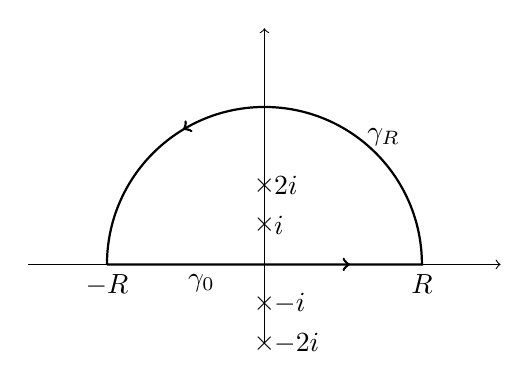
\begin{tikzpicture}
      \draw [->] (-3, 0) -- (3, 0);
      \draw [->] (0, -1) -- (0, 3);

      \draw [black, thick, ->-=0.3, ->-=0.8] (-2, 0) -- (2, 0) node [pos=0.3, below] {$\gamma_0$} arc(0:180:2) node [pos=0.3, right] {$\gamma_R$};

      \node [below] at (-2, 0) {$-R$};
      \node [below] at (2, 0) {$R$};

      \node at (0, 0.5) {$\times$};
      \node [right] at (0, 0.5) {$i$};
      \node at (0, -0.5) {$\times$};
      \node [right] at (0, -0.5) {$-i$};
      \node at (0, 1) {$\times$};
      \node [right] at (0, 1) {$2i$};
      \node at (0, -1) {$\times$};
      \node [right] at (0, -1) {$-2i$};
    \end{tikzpicture}
  \end{center}
The individual contour contributions are
$$\lim_{R\rightarrow\infty}\int_{\gamma_0}\frac{1}{(z^2+1)(z^2+4)}dz=\lim_{R\rightarrow\infty}\int_{-R}^R\frac{1}{(x^2+1)(x^2+4)}dx=\int_{-\infty}^\infty\frac{1}{(x^2+1)(x^2+4)}dx$$
$$\lim_{R\rightarrow\infty}\int_{\gamma_R}\frac{1}{(z^2+1)(z^2+4)}dz=\lim_{R\rightarrow\infty}\int_0^{\pi/2}\frac{iRe^{i\theta}d\theta}{(R^2e^{2i\theta}+1)(R^2e^{i2\theta}+4)}=\lim_{R\rightarrow\infty}O(R^{-3})=0$$
So as $R\rightarrow\infty$,
$$\oint_C\frac{1}{(z^2+1)(z^2+4)}dz=\int_{\gamma_0}\frac{1}{(z^2+1)(z^2+4)}dz+\int_{\gamma_R}\frac{1}{(z^2+1)(z^2+4)}dz\rightarrow\int_{-\infty}^\infty\frac{dx}{(x^2+1)(x^2+4)}$$
The poles enclosed are $z=2i$ and $z=i$ with residues
$$\res_{z=i}\frac{1}{(z^2+1)(z^2+4)}=\lim_{z\rightarrow i}\frac{z-i}{(z^2+1)(z^2+4)}=\lim_{z\rightarrow i}\frac{1}{2z(z^2+4)}=-\frac{i}{6}$$
$$\res_{z=2i}\frac{1}{(z^2+1)(z^2+4)}=\lim_{z\rightarrow 2i}\frac{z-2i}{(z^2+1)(z^2+4)}=\lim_{z\rightarrow 2i}\frac{1}{2z(z^2+1)}=\frac{i}{12}$$
Hence, by residue theorem,
$$\int_{-\infty}^\infty \frac{1}{(x^2+1)(x^2+4)}dx=2\pi i(-i/6+i/12)=\frac{\pi}{6}$$
\item Consider integrating along the unit circle $\gamma:~z=e^{i\theta},~\theta\in[0,2\pi)$. 
$$\int_0^{2\pi}\frac{d\theta}{5-3\sin\theta}=\oint_\gamma\frac{dz}{iz}\frac{1}{5-3(1/2i)(z-z^{-1})}=\frac{1}{i}\oint_\gamma\frac{dz}{5z-(3/2i)(z^2-1)}=\frac{-2}{3}\oint_\gamma\frac{dz}{(z-3i)(z-(i/3))}$$
 \begin{center}
    \begin{tikzpicture}
      \draw [->] (-3, 0) -- (3, 0);
      \draw [->] (0, -3) -- (0, 3);
      \draw [black, thick, ->-=0.2,->-=0.7] circle [radius=1.8];
      \node [right] at (1.2726, 1.2726) {$\gamma$};

      \node (z-) at (0, 2.1) {$\times$};
      \node [left] at (z-) {$3i$};

      \node (z+) at (0, 0.7) {$\times$};
      \node [left] at (z+) {$i/3$};

    \end{tikzpicture}
  \end{center}
  The integrand has poles at $z=3i$ and $z=i/3$, but only the latter is enclosed in the unit circle. The residue is
  $$\res_{z=i/3}\frac{-2}{3(z-3i)(z-(i/3))}=\lim_{z\rightarrow i/3}\frac{-2}{3(z-3i)}=\frac{-i}{4}$$
  Using residue theorem,
  $$\int_0^{2\pi}\frac{d\theta}{5-3\sin\theta}=2\pi i\frac{-i}{4}=\frac{\pi}{2}$$
 \end{enumerate}
\end{enumerate}
\end{ans}
\newpage
\begin{qns}[Transform Methods]\leavevmode
\begin{enumerate}[label=(\alph*)]
\item 
Using contour integration methods, show that for any complex number $a$
$$\int_{-\infty}^\infty e^{-(u+a)^2}du=\sqrt{\pi}$$
[Hint: You may use the fact that $\int_{-\infty}^\infty e^{-u^2}du=\sqrt{\pi}$.] \hfill\textbf{[6]}
\item The Fourier transform of a function $f(x)$ that satisfies $f(x)\rightarrow0$ as $|x|\rightarrow\infty$ is defined as
$$\tilde{f}(k)=\int_{-\infty}^\infty f(x)e^{-ikx}dx$$
Consider a function $u(x, t)$ that satisfies
$$\frac{\partial u}{\partial t}=\lambda\frac{\partial^2u}{\partial x^2}$$
Using Fourier transform methods, assuming that $u(x, t)\rightarrow 0$ as $|x|\rightarrow\infty$, show that the
solution is given by \hfill\textbf{[8]}
$$u(x,t)=\frac{1}{\sqrt{4\pi\lambda t}}\int_{-\infty}^\infty e^{-\frac{(x-y)^2}{4\lambda t}}u(y,0)dy$$
\item When $u(y,0)=\frac{a}{\sqrt{\pi}}e^{-\alpha^2y^2}$, with $\alpha>0$, show that $u(x,t)=\frac{\beta}{\sqrt{\pi}}e^{-\beta^2x^2}$ for a $\beta$ that you should specify in terms of $\alpha$, $\lambda$ and $t$. What happens to $u(y, 0)$ and $u(x, t)$ when $\alpha\rightarrow+\infty$?\hfill\textbf{[6]}
\end{enumerate}
\end{qns}
\begin{ans}\leavevmode
\begin{enumerate}[label=(\alph*)]
\item $e^{z}$ has essential pole at $z=\infty$. Construct a rectangular contour $\gamma$ with vertices at $z=\pm R,\pm R+i\text{Im}[a]$. No poles are enclosed here. 
  \begin{center}
    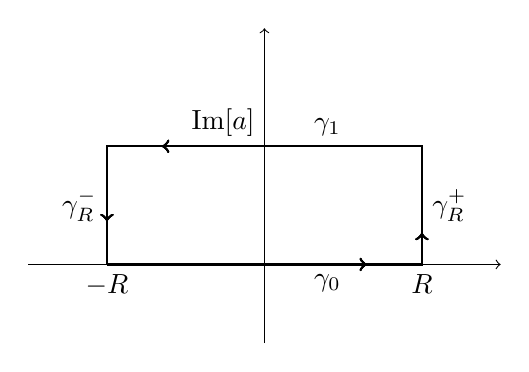
\begin{tikzpicture}
      \draw [->] (-3, 0) -- (3, 0);
      \draw [->] (0, -1) -- (0, 3);

      \draw [black, thick, ->-=0.3, ->-=0.4,->-=0.8,->-=0.95] (-2, 0) node [below] {$-R$} -- (2, 0) node [pos=0.7, below] {$\gamma_0$} node [below] {$R$} -- (2, 1.5) node [pos=0.5, right] {$\gamma_R^+$} -- (-2, 1.5) node [pos=0.3, above] {$\gamma_1$} -- (-2, 0) node [pos=0.5, left] {$\gamma_R^-$};


      \node [circle] at (0, 1.5) {};
      \node [anchor = south east] at (0, 1.5) {$\text{Im}[a]$};
    \end{tikzpicture}
  \end{center}
 The contributions along $\gamma_R^\pm$ is
 $$\int_{\pm R}^{\pm R+\text{Im}[a]}e^{-R^2-2iy+y^2}dy=O(e^{-R^2})\rightarrow 0,\text{ as }R\rightarrow\infty$$
 Let $u=R+iy$, then 
 $$\int_{-\infty}^{\infty+\text{Im}[a]}e^{-z^2}dz=\int_{-\infty}^\infty e^{-(u+i\text{Im}[a])^2}du=\int_{-\infty}^\infty e^{-(u+a)^2}du$$
 The contributions along $\gamma_0$ gives
 $$\int_{-R}^Re^{-x^2}dx\rightarrow\sqrt{\pi},\text{ as }R\rightarrow\infty$$
 Hence, by residue theorem, we must have
 $$\int_{-\infty}^\infty e^{-(u+a)^2}du=\sqrt{\pi}$$
\item Assuming $u(x,t),\frac{\partial u}{\partial x}\rightarrow0$ as $|x|\rightarrow\infty$, then the Fourier transforms of $\frac{\partial u}{\partial t}$, $\frac{\partial u}{\partial x}$ and $\frac{\partial^2u}{\partial x^2}$ give $\frac{\partial\tilde{u}}{\partial t}$, $ik\tilde{u}$, $-k^2\tilde{u}$ respectively. Hence, the Fourier transform of the PDE is
$$\frac{\partial\tilde{u}}{\partial t}=-k^2\lambda\tilde{u}\implies\tilde{u}(k,t)=A(k)e^{-\lambda k^2t}$$
where $A(k)=\tilde{u}(k,0)=\int_{-\infty}^\infty u(y,0)e^{-iky}dy$. The solution after inverse Fourier transform gives
$$u(x,t)=\frac{1}{2\pi}\int_{-\infty}^\infty A(k)e^{-\lambda k^2t}e^{ikx}dk=\frac{1}{2\pi}\int_{-\infty}^\infty\int_{-\infty}^\infty u(y,0)e^{-iky}e^{-\lambda k^2t}e^{ikx}dkdy$$
but $-\lambda k^2t+ik(x-y)=-\lambda t[(k-\frac{i}{2\lambda t}(x-y))^2+\frac{(x-y)^2}{4\lambda^2t^2}]$, hence we could have written
$$\int_{-\infty}^\infty e^{ik(x-y)-\lambda k^2t}dk=e^{-\frac{(x-y)^2}{4\lambda t}}\int_{-\infty}^\infty e^{-\lambda t(k-k_0)^2}dk=e^{-\frac{(x-y)^2}{4\lambda t}}\sqrt{\frac{\pi}{\lambda t}}$$
This is also the Green's function (fundamental solution for the PDE) $G(x-y,\lambda,t)$. Hence, the solution is
$$u(x,t)=\frac{1}{2\sqrt{\pi\lambda t}}\int_{-\infty}^\infty e^{-\frac{(x-y)^2}{4\lambda t}}u(y,0)dy$$
\item Now we have
$$u(x,t)=\frac{1}{\sqrt{4\pi\lambda t}}\frac{\alpha}{\sqrt{\pi}}\int_{-\infty}^\infty e^{-\frac{(x-y)^2}{4\lambda t}-\alpha^2y^2}dy$$
but 
$$-\alpha^2y^2-\frac{(x-y)^2}{4\lambda t}=-\frac{1+4\alpha\lambda t}{4\lambda t}(y-y_0)^2-\frac{\alpha}{1+4\alpha\lambda t}x^2$$
where $y_0=\frac{x}{1+4\alpha\lambda t}$. Evaluating the solution:
\begin{align}
    u(x,t)&=\frac{\alpha}{2\pi\sqrt{\lambda t}}\int_{-\infty}^\infty e^{-\frac{1+4\alpha\lambda t}{4\lambda t}(y-y_0)^2}dy~ e^{-\frac{\alpha}{1+4\alpha\lambda t}x^2}\nonumber\\&=\frac{\alpha}{2\pi\sqrt{\lambda t}}\sqrt{\frac{4\lambda t\pi}{1+4\alpha\lambda t}}e^{-\alpha x^2/(1+4\alpha\lambda t)}\nonumber\\&=\frac{\alpha}{\sqrt{\pi}(1+4\alpha\lambda t)}e^{-\alpha x^2/(1+4\alpha\lambda t)}\nonumber
\end{align}
where $\beta=\frac{\alpha}{1+4\alpha\lambda t}$. As $\alpha\rightarrow\infty$, $u(y,0)$ behaves like a delta function. $u(x,t)$ is a spreading Gaussian with variance $2\lambda t$. This is expected for the solutions of this type of PDE, known as the heat equation.
\end{enumerate}
\end{ans}
\newpage
\begin{qns}[Tensors]\leavevmode
\begin{enumerate}[label=(\alph*)]
\item Explain what is meant by an order $n$ Cartesian tensor and what it means for such a tensor to be isotropic.\\[5pt]
Show that the only isotropic tensors of order 2 are of the form $a\delta_{ij}$, where $a$ is a scalar. State (without proof) the most general form of an isotropic tensor of order 3.\hfill\textbf{[9]}
\item Let $\mathbf{n_1}$, $\mathbf{n_2}$, $\mathbf{n_3}$, $\mathbf{n_4}$ be unit vectors in $\mathbb{R}^3$. Let $V$ be the volume between two spheres with centres at the origin and radii $R_1$ and $R_2$, where $R_1 < R_2$.\\[5pt]
Justifying your answers carefully, obtain expressions for:
\begin{enumerate}[label=(\roman*)]
    \item $\int_V(\mathbf{x}\cdot\mathbf{n_1})(\mathbf{x}\cdot\mathbf{n_2})d^3x$;
    \item $\int_V(\mathbf{x}\cdot\mathbf{n_1})(\mathbf{x}\cdot\mathbf{n_2})(\mathbf{x}\cdot\mathbf{n_3})d^3x$;
    \item $\int_V(\mathbf{x}\cdot\mathbf{n_1})(\mathbf{x}\cdot\mathbf{n_2})(\mathbf{x}\cdot\mathbf{n_3})(\mathbf{x}\cdot\mathbf{n_4})d^3x$;
\end{enumerate}
\end{enumerate}
[ Hint: You may assume that the only isotropic tensors of order 4 are of the form $c\delta_{ij}\delta_{kl}+d\delta_{ik}\delta_{jl}+e\delta_{il}\delta_{jk}$, where $c$, $d$ and $e$ are scalars. ]\hfill\textbf{[11]}
\end{qns}
\begin{ans}\leavevmode
\begin{enumerate}[label=(\alph*)]
\item An $n$th-order Cartesian tensor $T$ is an object that is the same in all frames related by an orthogonal transformation. The tensor's components $T_{i_1i_2...i_n}$ with respect to two such frames related by such an orthogonal transformation (given by matrix $L$) must change as 
$$T_{i_1i_2...i_n}'=(\det L)^pL_{i_1j_1}L_{i_2j_2}L_{i_3j_3}...L_{i_nj_n}T_{j_1j_2...j_n}$$
where $p=1$ for pseudotensors and $p=0$ otherwise.\\[5pt]
An isotropic tensor has its components to be the same in all frames, i.e. $T_{ijk...}'=T_{\alpha\beta\gamma...}$.\\[5pt]
Consider the $n$-dimensional second-order tensor. Let's rotate around $x_1$-$x_2$ plane by $\frac{\pi}{2}$:
$$L^{(12)}=\begin{pmatrix}0&1\\-1&0\\\end{pmatrix}\oplus I_{(n-2)\times(n-2)}$$
Then, 
$$T_{ij}'=L_{ip}^{(12)}T_{pq}L_{jq}^{(12)}=(LTL^T)_{ij}=\begin{pmatrix}T_{22}&-T_{21}&T_{23}&\dots\\-T_{12}&T_{11}&-T_{13}&\dots\\T_{32}&-T_{31}&T_{33}&\dots\\\vdots&\vdots&\vdots&\ddots\\\end{pmatrix}$$
Then, for $T'=T$, we have $T_{11}=T_{22}$, $T_{12}'=-T_{21}=T_{21}'=-T_{12}\implies T_{12}=T_{21}=0$. Similar for $T_{1i}$, $T_{2i}$, $T_{i1}$ and $T_{i2}$. In general, use $L^{(mn)}$ rotate in the $x_m$-$x_n$ plane, all diagonal elements are identical and all off-diagonal elements must be zero, i.e. $T_{ij}=\lambda\delta_{ij}$ for some scalar $\lambda$.
\item Note that $V$ is spherically symmetric.
\begin{enumerate}[label=(\roman*)]
    \item $(\mathbf{n_1})_i(\mathbf{n_2})_j\int_Vx_ix_jd^3x$ is an isotropic second-order tensor, which is $\lambda\delta_{ij}$. Contracting this, we have
    $$\lambda\delta_{ii}=3\lambda=\int_Vx_ix_id^3x=\int_{R_1}^{R_2}\int_0^\pi\int_0^{2\pi}r^2r^2\sin\theta d\phi d\theta dr=\frac{4\pi}{5}(R_2^5-R_1^5)$$
    Then we must have
    $$\int_V(\mathbf{x}\cdot\mathbf{n_1})(\mathbf{x}\cdot\mathbf{n_2})d^3x=\frac{4\pi}{15}(R_2^5-R_1^5)\mathbf{n_1}\cdot\mathbf{n_2}$$
    \item $(\mathbf{n_1})_i(\mathbf{n_2})_j(\mathbf{n_3})_k\int_Vx_ix_jx_kd^3x$ is an isotropic third-order tensor. But, there is no such thing, hence the integral is just zero. Note, $\epsilon_{ijk}$ may be third-order and isotropic, but it is a pseudo-tensor.
    \item $(\mathbf{n_1})_i(\mathbf{n_2})_j(\mathbf{n_3})_k(\mathbf{n_4})_l\int_Vx_ix_jx_kx_ld^3x$ is an isotropic fourth-order tensor, which is $c\delta_{ij}\delta_{kl}+d\delta_{ik}\delta_{jl}+e\delta_{il}\delta_{jk}$, as given. Contracting this pairwise, either by $(j=i,k=l)$, $(j=l,i=k)$ or $(j=k,i=l)$, then for the first possibility, we have
    $$9c+3d+3e=\int_V|\mathbf{x}|^2|\mathbf{x}|^2d^3x=\int_{R_1}^{R_2}\int_0^\pi\int_0^{2\pi}r^4r^2\sin\theta d\phi d\theta dr=\frac{4\pi}{7}(R_2^7-R_1^7)$$
    For the other permutations, we have $3c+9d+3e$ and $3c+3d+9e$. Hence, $c=d=e$, then we must have
    $$\int_V(\mathbf{x}\cdot\mathbf{n_1})(\mathbf{x}\cdot\mathbf{n_2})(\mathbf{x}\cdot\mathbf{n_3})(\mathbf{x}\cdot\mathbf{n_4})d^3x=\frac{4\pi}{105}(R_2^7-R_1^7)[(\mathbf{n_1}\cdot\mathbf{n_2})(\mathbf{n_3}\cdot\mathbf{n_4})+(\mathbf{n_1}\cdot\mathbf{n_3})(\mathbf{n_2}\cdot\mathbf{n_4})+(\mathbf{n_1}\cdot\mathbf{n_4})(\mathbf{n_3}\cdot\mathbf{n_2})]$$
\end{enumerate}
\end{enumerate}
\end{ans}
\begin{qns}[Normal Modes]\leavevmode
\begin{enumerate}[label=(\alph*)]
\item A system has $n$ degrees of freedom and undergoes small oscillations about an equilibrium point. Write down the general form of its Lagrangian in generalised coordinates, explaining any approximations used. Give the equations of motion, and explain what is meant by a normal mode, a normal frequency and a zero mode of the system. \hfill\textbf{[4]}
\item Three beads of mass $m$, $m$ and $2m$ are joined pairwise by identical ideal springs of spring constant $k$, with the masses and springs constrained to lie on a frictionless circular hoop of radius 1. The hoop is fixed and lies in a horizontal plane. Obtain the kinetic and potential energies of the system in terms of suitable generalized coordinates. Obtain the normal modes and normal frequencies. Briefly describe each normal mode physically.\hfill\textbf{[9]}
\item At time $t = 0$ the masses are equally spaced around the hoop. The beads of mass $m$ are at rest, and the bead of mass $2m$ is given a small initial angular velocity $\Omega$. Obtain an equation for the state of the system at later times $t > 0$. \hfill\textbf{[7]}
\end{enumerate}
\end{qns}
\begin{ans}\leavevmode
\begin{enumerate}[label=(\alph*)]
\item If each particle can be described by a generalized coordinate $q_i$, then assuming there are no velocity-dependent potentials and the kinetic energies are quadratic in the speeds, the Lagrangian is the kinetic energy minus the potential energy $\mathcal{L}=T-V$, and has the form
$$\mathcal{L}(\mathbf{q},\mathbf{\dot{q}},t)=\sum_{i=1}^n\frac{1}{2}T_{ij}(t)\dot{q}_i\dot{q}_j-V(\mathbf{q},t)$$
If we further assume $\mathcal{L}$ to be time-independent and expand the potential around equilibrium positions (minima) to get
$$\mathcal{L}\approx\sum_{i=1}^n\frac{1}{2}T_{ij}\dot{q}_i\dot{q}_j-\sum_{i=1}^n\frac{1}{2}\frac{\partial^2V}{\partial q_i\partial q_j}q_iq_j$$
unique up to an additive constant (potential at the equilibrium position), which we can set to zero without loss of generality. Also, we assumed for any principal directions for which $V_{ij}$ has a zero eigenvalue, all subsequent derivatives are also zero. When the Lagrangian $\mathcal{L}$ is extremized, it satisfies the Euler-Lagrange equations $\frac{d}{dt}\frac{\partial\mathcal{L}}{\partial\dot{q}_i}=\frac{\partial\mathcal{L}}{\partial q_i}$ to give the equations of motion
$$\frac{d}{dt}T_{ij}\dot{q}_j=-V_{ij}q_j$$
A normal mode is a solution to this generalized eigenvalue of the form $\mathbf{q}=\mathbf{q_0}e^{i\omega t}$ or $\mathbf{q}=\mathbf{a}+t\mathbf{b}$
, where latter is known as the zero mode. To find the normal mode frequencies, we solve the matrix equation
$$\omega^2T\mathbf{q}=-V\mathbf{q}$$
and for each $\omega=0$, we need a linearly independent zero mode.
\item Our coordinates will be the angles that the bead make from their equilibrium positions. If the natural lengths of the springs happen to be not $\frac{2\pi}{3}$, then at equilibrium, this merely adds a constant term to the potential energy, which will not affect the equations of motion. The potential energy and kinetic energy are thus respectively
$$V=\frac{1}{2}k(\theta_1-\theta_2)^2+\frac{1}{2}k(\theta_2-\theta_3)^2+\frac{1}{2}k(\theta_3-\theta_1)^2=\frac{1}{2}k\begin{pmatrix}\theta_1&\theta_2&\theta_3\\\end{pmatrix}\begin{pmatrix}2&-1&-1\\-1&2&-1\\-1&-1&2\\\end{pmatrix}\begin{pmatrix}\theta_1\\\theta_2\\\theta_3\\\end{pmatrix}$$
$$T=\frac{1}{2}m\dot{\theta}^2+\frac{1}{2}m\dot{\theta}_2^2+\frac{1}{2}2m\dot{\theta}_3^2=\frac{1}{2}m\begin{pmatrix}\dot{\theta}_1&\dot{\theta}_2&\dot{\theta}_3\\\end{pmatrix}\begin{pmatrix}1&0&0\\0&1&0\\0&0&2\\\end{pmatrix}\begin{pmatrix}\dot{\theta}_1\\\dot{\theta}_2\\\dot{\theta}_3\\\end{pmatrix}$$
Let $V=0.5k\boldsymbol{\theta}^T\mathcal{V}\boldsymbol{\theta}$ and $T=0.5m\boldsymbol{\dot{\theta}}^T\mathcal{T}\boldsymbol{\dot{\theta}}$. We thus solve for $0=\det(\mathcal{V}-m\omega^2\mathcal{T})$:
$$0=\det\begin{pmatrix}2k-m\omega^2&-k&-k\\-k&2k-m\omega^2&-k\\-k&-k&2k-2m\omega^2\\\end{pmatrix}=(2k-m\omega^2)((2k-m\omega^2)(2k-2m\omega^2)-k^2)-2k^2(3k-2m\omega^2)$$
which have solutions $\omega^2=0$, $\omega^2=\frac{k}{m}$ and $\omega^2=\frac{2k}{m}$. By inspection, the eigenvector for the zero mode is $(1,1,1)^T$, i.e. rotation with constant angular velocity. For $\omega^2=\frac{k}{m}$, the eigenvector is $(1,-1,0)^T$, with the lighter masses moving in anti-phase with respect to each other, but the heavier mass stationary. For $\omega^2=\frac{2k}{m}$, the eigenvector is $(1,1,-1)^T$, with the lighter masses moving in phase, but in anti-phase with the heavier mass.
\item The general solution is
$$\boldsymbol{\theta}(t)=\begin{pmatrix}\theta_1\\\theta_2\\\theta_3\\\end{pmatrix}=(c_1+c_2t)\begin{pmatrix}1\\1\\1\\\end{pmatrix}+\text{Re}[c_3e^{i\omega_0t}]\begin{pmatrix}1\\-1\\0\\\end{pmatrix}+\text{Re}[c_4e^{i\sqrt{2}\omega_0t}]\begin{pmatrix}1\\1\\-1\\\end{pmatrix}$$
where $\omega_0=\sqrt{\frac{k}{m}}$. The initial conditions are $\boldsymbol{\theta}(t=0)=(\theta_0,\theta_0,\theta_0)^T$ and $\boldsymbol{\dot{\theta}}(t=0)=(0,0,\Omega)^T$. By inspecton, we see that $c_1=\theta_0$ and $c_3,c_4$ to be purely imaginary.
$$\boldsymbol{\dot{\theta}}(t=0)=\begin{pmatrix}0\\0\\\Omega\\\end{pmatrix}=c_2\begin{pmatrix}1\\1\\1\\\end{pmatrix}+\text{Re}[i\omega_0c_3]\begin{pmatrix}1\\-1\\0\\\end{pmatrix}+\text{Re}[i\sqrt{2}\omega_0c_4]\begin{pmatrix}1\\1\\-1\\\end{pmatrix}$$
Exploiting the orthogonality of the eigenvectors with respect to $\mathcal{T}=m\diag(1,1,2)$,
$$c_2\langle(1,1,1)^T|(1,1,1)^T\rangle_{\mathcal{T}}=\langle(0,0,\Omega)^T|(1,1,1)^T\rangle_{\mathcal{T}}\implies 2\Omega=4c_2$$
$$-\omega_0\text{Im}[c_3]\langle(1,-1,0)^T|(1,-1,0)^T\rangle_{\mathcal{T}}=\langle(0,0,\Omega)^T|(1,-1,0)^T\rangle_{\mathcal{T}}\implies c_3=0$$
$$-\sqrt{2}\omega_0\text{Im}[c_4]\langle(1,1,-1)^T|(1,1,-1)^T\rangle_{\mathcal{T}}=\langle(0,0,\Omega)^T|(1,1,-1)^T\rangle_{\mathcal{T}}\implies 4\sqrt{2}\omega_0c_4=-2\Omega$$
Hence,
$$\boldsymbol{\theta}(t)=(\theta_0+0.5\Omega t)\begin{pmatrix}1\\1\\1\\\end{pmatrix}-\frac{\Omega}{2\sqrt{2k/m}}\sin\sqrt{2k/m}t\begin{pmatrix}1\\1\\-1\\\end{pmatrix}$$
\end{enumerate}
\end{ans}
\newpage
\begin{qns}[Group Theory]\leavevmode
\begin{enumerate}[label=(\alph*)]
\item Give the axioms for a group $G$. Explain what is meant by saying that $H$ is a subgroup of $G$ and that $\{g_1, . . . , g_n\}$ is a set of generators for $G$. Explain what is meant by the order of $G$ and the order of an element $g$ of $G$, and state Lagrange’s theorem. Explain what is meant by a cyclic group and an isomorphism between groups.\hfill\textbf{[6]}
\item Now suppose $G$ is a group of order 8. What are the possible orders of its elements? Show that if $G$ has no elements of order greater than 2 then it is a direct product of cyclic groups.\\[5pt] [Hint: The direct product of groups $G_1$, $G_2$, . . . , $G_n$ is the group with elements $(g_1, g_2, . . . , g_n)$ (where $g_i\in G_i$), with identity $(I_{G_1} , . . . , I_{G_n})$, where $I_{G_i}$ is the identity of $G_i$. The group multiplication is defined by $(g_1, . . . , g_n)(g_1', . . . , g_n') = (g_1g'_1, . . . , g_ng'_n)$ and the inverse by $(g_1, . . . , g_n)^{−1} = (g^{−1}_1 , . . . , g^{−1}_n )$.]\hfill\textbf{[5]}
\item Now suppose that $G$ has order 8 and is generated by elements $a$ and $b$ which have orders 4 and 2 respectively. Show that either (i) $ab = ba$ or (ii) $ab = ba^3$. Show that in case (i) $G$ is uniquely defined up to isomorphism. Show that in case (ii) $G$ is also uniquely defined up to isomorphism, and give a geometric representation of $G$ and the generators $a$ and $b$ in this case. \hfill\textbf{[7]}
\item Is the group identified in part (c)(ii) the only non-abelian group of order 8? Justify your answer carefully.\hfill\textbf{[2]}
\end{enumerate}
\end{qns}
\begin{ans}\leavevmode
\begin{enumerate}[label=(\alph*)]
\item A group $G$ is a set of elements with a binary operation defined for $g_1,g_2\in G$ such that $g_1*g_2$ and the resultant group elements satisfy
\begin{itemize}
    \item closure: $g_i*g_j\in G$ $\forall g_i,g_j\in G$.
    \item associative: $(g_i*g_j)*g_k=g_i*(g_j*g_k)$ $\forall g_i,g_j,g_k\in G$.
    \item identity: $\exists e\in G$ such that $e*g_i=g_i$ $\forall g_i\in G$.
    \item inverse: for every $g_i\in G$, $\exists g_i'\in G$ such that $g_i*g_i'=e$.
\end{itemize}
$H$ is a subgroup, i.e. $H\leq G$ if it is a subset that also obeys the above axioms.\\[5pt]
A set of generators for a group $G$ is a (not necessarily unique) set of elements in $G$ such that every element in $G$ can be found by combining the generators with each other to various powers. All non-identical sets of generators contain the same number of elements, and the set is minimal in that if you removed any one generator, then the set would not generate all of $G$.\\[5pt]
The order of a group $G$ is $|G|$, the number of elements it contains. The order of an element $g\in G$ is the minimum positive integer number of times you need to combine it with itself to return the identity, i.e. if $\ord(g)=k$, then $g^k=e$.\\[5pt]
Lagrange's theorem states that the order of a subgroup is a factor of the order of the parent group.\\[5pt]
A cyclic group has a single generator (not necessarily unique).\\[5pt]
A homomorphism between two groups $G$ and $H$ is a mapping $\Phi:~G\rightarrow H$ such that the group structure is preserved, i.e. $\Phi(g_i)\Phi(g_j)=\Phi(g_i*g_j)$ $\forall g_i,g_j\in G$.
\item If $g\in G$, then by Lagrange's theorem, $\ord(g)$ (order of the resultant generator) are factors of 8: 1,2,4, 8. If every element other than the identity is of order 2, then it can be written as a direct product of $C_2=\{e,a\}$, say $C_2\times C_2\times C_2$. Let the elements be
$$I=(e_1,e_2,e_3),\quad A=(e_1,e_2,a_3),\quad B=(e_1,a_2,e_3),\quad C=(a_1,e_2,e_3)$$
where $A^2=B^2=C^2=I$, $A$, $B$ and $C$ act as generators for this group. We have $AB=BA=(e_1,a_2,a_3)$, $AC=CA=(a_1,e_2,a_3)$, $BC=CB=(a_1,a_2,e_3)$, $ABC=(a_1,a_2,a_3)$, which are all (8 of them) in $C_2\times C_2\times C_2$. Also, we have established that this is an abelian group.
\item We have $\ord(a)=2$, $\ord(b)=4$. Consider $g=a^pb^q$, with $p$ only meaningful modulo 2 and $q$ only meaningful modulo 4. Is $ab$ distinct from $a$, $b$ and $I$?\\[5pt]
If $ab=I$, then $b=a^{-1}$. But $\ord(a)=2$, so $a=a^{-1}=b$, but a set of generators has distinct elements, so contradict. Hence, $ab\neq I$.\\[5pt]
No generator is the identity as a set of elements that generated the entire group which contains the identity would still generate entire group after removing the identity. Such a set would not be minimal, so contradict. $ab\neq a$, $ab\neq b$.\\[5pt]
We could thus generate more elements, namely $ab^2$, $b^2$, $b^3$ and $ab^3$. An alternative generator is $\{I,a,b,ba,b^2,b^2a,b^3,b^3a\}$ and this must be the same set, so $\{ab,ab^2,ab^3\}$ and $\{ba,b^2a,b^3a\}$ must be the same set (just reordered). The order is not 8 since the group will have a generating set of size 1. Also, these elements are not identity and again must have order 2 or 4. Consider the following combinations:
\begin{itemize}
    \item $ab=ba\implies ab^2=b^2a,~ab^3=b^3a$ no contradiction.
    \item $ab=b^2a\implies(ab)^2=ab^3a,~(ab)^4=ab^2a$, a contradiction since $\ord(ab)$ is neither 2 nor 4.
    \item $ab=b^3a\implies (ab)^2=I$, this is of order 2 and no contradiction.
    \item $ab^2=ba\implies(ab^2)^2=ab^2ab^2=ab^2ba=ab^3a,~(ab^2)^4=ab^2a$. A contradiction again since $\ord(ab^2)$ is neither 2 nor 4.
\end{itemize}
Both allowed case: map $b\rightarrow b^3$. This is isomorphic to the symmetry group of a square, i.e. $D_4$. $a$ is geometrically a reflection about the diagonal and $b$ is the rotation of magnitude $\frac{\pi}{2}$ about the centre of the square in the plane of the square.
\item No. The quaternion group has two order four generators and has eight elements. But this was not considered in part (c) as it is non-abelian.
\end{enumerate}
\end{ans}
\begin{qns}[Group Theory]\leavevmode
\begin{enumerate}[label=(\alph*)]
\item Define a homomorphism between groups $G$ and $G'$. Define what is meant by the kernel of a homomorphism and by a normal subgroup $H$ of a group $G$.\hfill\textbf{[4]}
\item Consider the set of matrices of the form
$$M=\begin{pmatrix}a&b\\0&1\\\end{pmatrix}$$
where $a$ and $b$ are complex and $a\neq 0$. Show that this set forms a group $G$ under matrix multiplication. Let $G'$ be the subset of $G$ such that $b = 0$. Show that $G'$ is a subgroup of $G$ and that the map 
$$f:\begin{pmatrix}a&b\\0&1\\\end{pmatrix}\rightarrow\begin{pmatrix}a&0\\0&1\\\end{pmatrix}$$
defines a homomorphism.\hfill\textbf{[8]}
\item Hence, or otherwise, identify a non-trivial normal subgroup of $G$ and show that it is a normal subgroup.\hfill\textbf{[8]}
\end{enumerate}
\end{qns}
\newpage
\begin{ans}\leavevmode
\begin{enumerate}[label=(\alph*)]
\item If $G$ and $G'$ are groups, then the mapping $\Phi:~G\rightarrow G'$ is a group homomorphism if $\forall~a,b\in G$,
$$\phi(a\cdot_Gb)=\phi(a)\cdot_{G'}\phi(b)$$
The kernel of the homomorphism is
$$\Ker\phi=\{h\in G|~\phi(h)=e_{G'}\text{ for some } h\in G\}$$
$H$ is a normal subgroup of $G$ if $g_iH=Hg_i$ $\forall g_i\in G$.
\item Check axioms of a group $G$:
\begin{itemize}
    \item closure: Consider $M,M'\in G$ 
    $$MM'=\begin{pmatrix}a&b\\0&1\\\end{pmatrix}\begin{pmatrix}a'&b'\\0&1\\\end{pmatrix}=\begin{pmatrix}aa'&ab'+b\\0&1\\\end{pmatrix}\in G$$
    which is true since $a,a'\neq 0\implies aa'\neq 0$.
    \item associative: matrix multiplication is associative.
    \item identity: in $G$ if $a=1\neq 0$ and $b=0$.
    \item inverse: $M^{-1}=\begin{pmatrix}a^{-1}&-ba^{-1}\\0&1\\\end{pmatrix}\in G$ since $a\neq0\implies a^{-1}\neq 0$.
\end{itemize}
When $b=0$, check the subgroup axioms for $G'$:
\begin{itemize}
    \item closure: $\begin{pmatrix}a'a&0\\0&1\\\end{pmatrix}\in G'$ obviously.
    \item associativity: inherited from $G$.
    \item identity: inherited as well.
    \item inverse: $\begin{pmatrix}a^{-1}&0\\0&1\\\end{pmatrix}\in G'$.
\end{itemize}
Check $f$ is a homomorphism:
\begin{align}
    f\bigg(\begin{pmatrix}a&b\\0&1\\\end{pmatrix}\begin{pmatrix}a'&b'\\0&1\\\end{pmatrix}\bigg)&=f\bigg(\begin{pmatrix}aa'&ab'b\\0&1\\\end{pmatrix}\bigg)\nonumber\\&=\begin{pmatrix}aa'&0\\0&1\\\end{pmatrix}\nonumber\\&=\begin{pmatrix}a&0\\0&1\\\end{pmatrix}\begin{pmatrix}a'&0\\0&1\\\end{pmatrix}\nonumber\\&=f\bigg(\begin{pmatrix}a&b\\0&1\\\end{pmatrix}\bigg)f\bigg(\begin{pmatrix}a'&b'\\0&1\\\end{pmatrix}\bigg)\nonumber
\end{align}
\item Consider the cyclic group $G':=C_2=\{g,e\}$ s.t. $a=e^{i\pi}=-1$, $b=0$, then $g\in C_2$ s.t. $g^2=e$. Check subgroup axioms of $G'\subseteq G$:
\begin{itemize}
    \item closure: $g^{p\text{ mod}2}\in G'$.
    \item associtivity: inherited from $G$.
    \item identity: $g^2=e\in G$.
    \item inverse: self-inverse.
\end{itemize}
The identity commutes with itself, so trivially it is in a conjugacy class of its own. 
$$gM_i-M_ig=\begin{pmatrix}-1&0\\0&1\\\end{pmatrix}\begin{pmatrix}a_i&b_i\\0&1\\\end{pmatrix}-\begin{pmatrix}a_i&b_i\\0&1\\\end{pmatrix}\begin{pmatrix}-1&0\\0&1\\\end{pmatrix}=\begin{pmatrix}-a_i&0\\0&1\\\end{pmatrix}-\begin{pmatrix}-a_i&0\\0&1\\\end{pmatrix}=0$$
$g$ commutes with all $M_i\in G$, so it is in a conjugacy class of its own. Hence, $G'=\{g,e\}\lhd G$ is a normal subgroup and it is constructed from a union of entire conjugacy classes.
\end{enumerate}
\end{ans}
\newpage
\begin{qns}[Representation Theory]\leavevmode
\begin{enumerate}[label=(\alph*)]
\item Define the permutation group $S_n$ of $n$ elements. Explain what is meant by an $m$-dimensional representation of a group $G$, by an irreducible representation of $G$, and by inequivalent representations of $G$.\hfill\textbf{[4]}
\item Describe the conjugacy classes of $S_4$, stating the number of elements in each. [You need not prove these are the conjugacy classes.]\hfill\textbf{[4]}
\item Describe two inequivalent one-dimensional representations of $S_4$, showing that they are representations. What are their kernels? Are the kernels subgroups? Justify your answers. What are the characters of the two representations? Verify that they are orthogonal. \hfill\textbf{[6]}
\item Obtain the dimensions of the inequivalent irreducible finite-dimensional representations of $S_4$, justifying your answer carefully. [You may quote without proof any relevant theorems, provided they are clearly stated.] \hfill\textbf{[6]}
\end{enumerate}
\end{qns}
\begin{ans}\leavevmode
\begin{enumerate}[label=(\alph*)]
\item The permutation group $S_n$ consists of the set of shufflings of $n$ elements.
$$\sigma=\begin{pmatrix}a&b&c&d&e\\\sigma(a)&\sigma(b)&\sigma(c)&\sigma(d)&\sigma(e)\\\end{pmatrix}$$
can be written in terms of cycles. It is conventional to omit single entry cycles in our notation.\\[5pt]
An $m$-dimensional representation of a group is a homomorphism to a set of $m$-dimensional invertible matrices. If $\exists$ a single similarity transform applied to all the matrices in the representation simultaneously that renders them all block diagonal, then the representation is reducible. Otherwise, the representation is irreducible. Equivalently, an irreducible representation has no non-trivial invariant subspaces. Two representations are equivalent if $\exists$ a single similarity transform that maps one set of matrices to the other. Otherwise, the two representations are not equivalent.
\item Permutation cycles of the same type are in the same conjugacy classes of $S_4$. $\Id$ is in a conjugacy class of its own. $(..)$ have 6 elements in its conjugacy class, all of them are their own inverse. $(...)$ have 8 elements in its conjugacy class. $(..)(..)$ have 3 elements in its conjugacy class, all of them are their own inverse. $(....)$ have 3 elements in its conjugacy class. The total number is $1+6+8+3+6=24=4!=|S_4|$.
\item Consider the trivial representation $I$. $\Ker(I(S_4))=S_4\leq S_4$. $\chi_I$ contains 24 copies of $+1$.\\[5pt]
Consider another one-dimensional representation $T$ where all elements containing an even number of pairwise swaps ($\Id$, $(...)$, $(..)(..)$) maps to 1, while an odd number of pairwise swaps ($(..)$, $(....)$) maps to $-1$. $\Ker T$ is thus the set of permutations decomposable into an even number of pairwise swaps. Trivially, this is closed, inherits associativity, contains $\Id$ and all appropriate inverses. So $T\leq S_4$. There is exactly 12 (half of $|S_4|$) elements that map to $+1$ and another 12 map to $-1$, so $\chi_T$ has 12 copies of $+1$ and 12 copies of $-1$. Hence, the characters are orthogonal:
$$\chi_T\cdot\chi_I=12(+1)+12(-1)=0$$
\item The number of inequivalent irreducible representations is the number of conjugacy classes which is 5. The sum of squares of dimensions of the irreducible representations is the order of the group which is 24. We thus look for 5 natural numbers that sum and square to 24. In part (c), we identified two distinct one-dimensional representations, so solve
$$l^2+m^2+n^2=22\implies l=2=m,~n=3$$
Hence, the dimensions of the irreducible representations are $1,1,2,3,3$.

\end{enumerate}
\end{ans}
\end{document}